\documentclass[twoside,12pt]{report}
	\usepackage[newparttoc]{titlesec}
\usepackage{titletoc}
%\usepackage{etoc}
%	\etocsettocstyle{}{}
\usepackage{pdfpages}
\usepackage{lipsum}
\usepackage[utf8]{vietnam}

\usepackage{xparse} % hỗ trợ định nghĩa options cho lệnh
\usepackage{xcolor,color,colortbl}  % các gói trộn màu 
\usepackage{xpatch}
\usepackage{tkz-tab} % xử lý hình với tikz 
\usepackage{fancybox} % tạo các hộp 
\usepackage[most]{tcolorbox} % định dạng các hộp, khung 
	\tcbuselibrary{skins} % thư viện bổ sung cho tcolorbox
\usepackage{graphicx} % Chèn hình, vẽ hình đơn giản 
%\usepackage{epstopdf} % chèn hình eps cho pdflatex 
%\usepackage{wrapfig} % Chèn hình giữa chữ
\usepackage{geometry} % định dạng, canh lề trang in 
\usepackage{indentfirst} % viết hoa đoạn đầu của mỗi mục 
\usepackage{fancyhdr} % tạo header và footer 
\usepackage{longtable} % bảng dài nhiều trang 
\usepackage[locale=DE]{siunitx} % cách viết số đo có đơn vị theo chuẩn DE (gần giống VN) 
\usepackage[T1,T5]{fontenc} % font encoding 
\usepackage{tikz} % gói TikZ vẽ hình 
	\usetikzlibrary{decorations.shapes,shapes.geometric,calc}
\usepackage[version=3]{mhchem} % công thức và phương trình hóa học 
%\usepackage{chemmacros} % công thức ion trong hóa học
%\usepackage{chemfig} % vẽ cấu trúc hợp chất hữu cơ 
%\usepackage{wasysym} % các ký hiệu sinh học, khoa học 
%\usepackage[printwatermark]{xwatermark} % watermark 
\usepackage{makecell} % hỗ trợ định dạng ô trong bảng 
\usepackage{array} % hỗ trợ định dạng array
\usepackage{amsmath,amssymb} % công thức và ký hiệu toán học 
%\usepackage{mathabx} % ký hiệu toán học bổ sung (+ thiên văn)  
\usepackage{enumitem}
	\setlist[itemize,enumerate,description]{noitemsep, {nosep}}
\usepackage{cprotect}% cho phép marco hủy tác dụng chống verbatim trong các môi trường tiêu đề 
\usepackage{multicol} % môi trường nhiều cột
\usepackage{environ} % hỗ trợ định nghĩa môi trường
\usepackage{tasks} % hỗ trợ list dạng task 
\usepackage{calc} % hỗ trợ tính toán & đo văn bản 
\usepackage{multido} % thực hiện lệnh lặp lại 
\usepackage{pgf} % hỗ trợ phép tính toán học và vẽ hình	
\usepackage{setspace} % hỗ trợ định dạng khoảng cách văn bản. 
%\usepackage{showframe}	% hiển thị khung lề 
\usepackage{tabularx} % hỗ trợ bảng 
\usepackage{needspace} % hỗ trợ định dạng khối dòng văn bản 
\usepackage{hyperref}
%
\hypersetup{hidelinks,colorlinks=false,breaklinks=true,bookmarksopen=true}
%\usepackage{slashbox}	% chia chéo trong bảng
%\usepackage{mnsymbol} % tạo thêm symbol (stars)

%\usepackage[varg]{txfonts}
%\usepackage{sectsty}
%\allsectionsfont{\sffamily}
%\usepackage{times}
\usepackage{helvet}

\usepackage{eso-pic,calc}
\listfiles

	%============ DECLARATION OF DEFAULT VALUE =====
	\newcommand{\outfooter}{
		Đề cương HK I - Vật lý 12 % Tên tài liệu ở footer
	}
	
	\graphicspath{{../figs/}{../extra/}} % các thư mục chứa hình ảnh 
	
% ========== PAPER FORMAT ====================
% --- paper size 
	\geometry{
		a4paper	% khổ giấy A4
		,total={170mm,247mm} % kích thước văn bản 170mmx247mm 
		,left=20mm % canh lề trái 
		,top=20mm % canh lề trên 
		,footskip=1.5cm % khoảng cách từ văn bản đến footer 
	}	
% --- line spacing -- choose 1 in 2 choices 
 	\onehalfspacing			% cách dòng đơn
	%\doublespacing			% cách dòng đôi  


% ========== DEFINE LEVELS  
% --- define \mychapter level, between \part and \chapter
	\titleclass{\mychapter}{top}[\part] 
	\newcounter{mychapter}[part]
	\renewcommand{\themychapter}{\arabic{mychapter}}
	%\titlespacing{\mychapter}{1pc}{*4}{*2.3}
	\titlespacing{\mychapter}{0pt}{1cm}{2.3em}
	
	
% ========== MAIN TABLE OF CONTENTS =========
	\contentsmargin{1.5em}
% Part text styling
%	\texorpdfstring{\setlength\fboxsep{0pt}\noindent\protect\colorbox{ocre!35}{\strut\protect\parbox[c][.8cm]{\linewidth}{\Large\sffamily\protect\centering #1\quad\mbox{}}}	
	\titlecontents{part}
		[3cm] % Left indentation
		{\addvspace{20pt}
			\begin{tikzpicture}[remember picture, overlay]%
			\draw[fill=black!60,draw=black!60] (-3.,-.1) ;%
			\pgftext[left,x=-2.5cm,y=0.23cm]{\color{black}\large\sc\bfseries Phần \thecontentslabel.};%
			\end{tikzpicture}\color{black!60}\large\bfseries
				} % Spacing and font options for parts
		{}
		{}
		{}
		[\addvspace{5pt}\color{black}]
% My chapter text styling 
	\titlecontents{mychapter}
		[1.25em]
		{}
		{\bfseries Bài \thecontentslabel.\enspace}
		{}
		{\bfseries\titlerule*[0.75pc]{.}\contentspage} %bad formatting, but only here to produce a content line in ToC	
% Chapter text styling
	\titlecontents{chapter}
		[1.25em] % Left indentation
		{\bfseries} % Spacing and font options for chapters
		{} % Formatting of numbered sections of this type
		{} % Formatting of numberless sections of this type
		{\bfseries\titlerule*[0.75pc]{.}\contentspage} % Formatting of the filler to the right of the heading and the page number

\makeatletter
% that a section has Level 2, rather than Level 1.
\renewcommand{\l@section}{\@dottedtocline{2}{1.5em}{2.3em}}
\makeatother
\setcounter{tocdepth}{1}


% ========== TITLE FORMATTING 
% --- draw circle around chapter number 
	\newcommand*{\circhap}[1]{
		\tikz[baseline=(char.base)] % tạo ô bao quanh chữ
		{
			\node[
			shape=circle % hình tròn
			,fill=gray!50 % màu nền 
			,inner sep=5pt % khoảng cách chữ và hình 
			] 
			(char)
			{#1};
		}
	}	
% --- 
\AtBeginDocument{
% --- PART format (level -1)
	\titleclass{\part}{top}
	\renewcommand{\thepart}{\Roman{part}}
	\titleformat{\part}
		[display]
		{\bfseries\Huge}
		{\filleft \LARGE PHẦN  \Huge\thepart}
		{4ex}
		{\titlerule
		 %\pagecolor{green}	 
		 \vspace{2ex}%
		 \filcenter
	 	}
		[\vspace{2ex}%
		 \titlerule
		 %\pagecolor{white}
		]
		
% --- MYCHAPTER format (level 0) 
	\titleformat{\mychapter}
		[display]
		{\bfseries\huge}
		{\filleft \LARGE\itshape Bài \Huge\themychapter}
		{4ex}
		{%\titlerule
			\vspace{2ex}%
			\filcenter}
		[\vspace{2ex}%
		%\titlerule
		]

% --- CHAPTER format (level 1)
	\titleformat{\chapter}
		[display]
		{\normalfont\large\bfseries\centering}
		{}
		{-2cm}
		{\Large}	
		%\titleformat % định dạng tiêu đề 
	\renewcommand{\thesection} % định dạng chỉ số subsection
		{
			\arabic{section} % kiểu số Ả rập 
		}
	\titleformat{\section} % chỉnh tiêu đề section  
		[hang]
		{\large\bfseries} % format 
		{\thesection\!\!.} % không ghi chỉ mục 
		{0.5em} % khoảng cách đến tiêu đề 
		{} % trước khi bắt đầu 
\renewcommand{\thesubsection} % định dạng chỉ số subsection
{
	\thesection\!\!.\,\arabic{subsection} % kiểu số Ả rập 
}
\titleformat % định dạng tiêu đề 
{\subsection} %command 
{\normalsize\bfseries} % format 
{\thesubsection\!\!.} % đánh số 1,2,3,...
{0.5em} % khoảng cách đến tiêu đề 
{} % trước tiêu đề 
[] % sau tiêu đề 	
\renewcommand{\thesubsubsection} % định dạng chỉ số subsubsection 
{
	\thesubsection\!\!.\,\arabic{subsubsection} % kiểu số Ả rập 
}
\titleformat % định dạng tiêu đề 
{\subsubsection} % command 
{\normalsize\bfseries} % format 
{\thesubsubsection\!\!.} % 1.1, 1.2
{0.25em} % khoảng cách sau 1.1 
{ } % trước tiêu đề 
[\vspace*{-3mm}] % sau tiêu đề  	
}


% ----- định dạng Header và footer
% --- trang văn bản thông thường  
\pagestyle{fancy} 
\fancyhf{}
\renewcommand{\headrulewidth}
{0pt} % độ dày đường kẻ ở header 
\newcommand*\cirpage[1] % tạo hình tròn quanh số trang 
{\tikz[baseline=(char.base)]
	{
		\node[
		shape=circle
		,draw=black
		,fill=gray!0
		,inner sep=2pt
		]
		(char)
		{#1};
	}
}
\fancyfoot[LO,RE] % footer - lề trong 
{	
	\small \outfooter % tên tài liệu lấy từ phần khai báo đầu file 
}  
\fancyfoot[CO,CE] % footer - giữa trang 
{
	\small \cirpage{\thepage}
} 
\fancyfoot[LE] % footer - lề ngoài 
{
	\vspace*{-11pt}
	\hspace*{-1.1pt}
\includegraphics[scale=0.03]{../extra/Logo.png} 
}
\fancyfoot[RO] % footer - lề ngoài 
{
	\vspace*{-11pt}
	
\includegraphics[scale=0.03]{../extra/Logo.png}\hspace*{-5pt}
}
% --- trang Part và Chapter title 
\fancypagestyle{plain} % mặc định của trang Part và Chapter title 
{
	\fancyfoot[LO,RE]
	{
		\small \outfooter
	}
	\fancyfoot[CO,CE]
	{
		\small \cirpage{\thepage}
	} % footer - giữa trang chẵn và lẻ 
	\fancyfoot[LE]
	{
		\vspace*{-11pt}
		\hspace*{-1.1pt}
\includegraphics[scale=0.03]{../extra/Logo.png}
	}
	\fancyfoot[RO]
	{
		\vspace*{-11pt}
		
\includegraphics[scale=0.03]{../extra/Logo.png}\hspace*{-5pt}
	}
} % giống với trang thường 


% --- Định dạng cấu trúc 
\setcounter{secnumdepth}{4} % đánh số đến cấp thứ 4 của chỉ mục (subsubsection sẽ được đánh số)






% ======== MANUAL DEFINITIONS VERSION 3.1415 ===
% --- chừa chỗ trống tương ứng - văn bản gốc 
\newcommand{\bltext}[1]{#1}
\newcommand{\xtrule}{ }
\newcommand{\phantomeqn}[2][b]{
	#2
}


% --- tạo hộp Tóm tắt lý thuyết  
\newcommand{\hops}[1] %lệnh hộp (tóm tắt lý thuyết)
{	
	\begin{flushright}
		\leavevmode 
		\begin{tcolorbox}
			[
			standard jigsaw
			,opacityback=0
			,opacityframe=1
			,breakable
			,pad at break*=2mm
			%						,colback=white!20!white,
			,colframe=black!70!white
			,width=\textwidth
			,before upper={\parindent15pt}
			%						,watermark color=blue!3!white
			%						,watermark text=\arabic{tcbbreakpart}
			]
			{
				#1
			}
		\end{tcolorbox}
	\end{flushright}
}

% --- định nghĩa môi trường mới - Dạng 
\newcounter{dang} % định nghĩa chỉ số cho Dạng 
[section] % chỉ số sẽ reset mỗi section 
\newenvironment % định nghĩa môi trường mới 
{dang} % tên môi trường 
[1] % số thành phần phải có 
{
	\refstepcounter{dang} % chỉ số tương ứng 
	\leavevmode
	\begin{center}
		\leavevmode \vspace{-0.6cm}
		\begin{tcolorbox}
			[
			bicolor
			,sidebyside
			,width=0.93\textwidth
			,lefthand width=2.7cm
			,arc=0.5cm
			%	,rounded corners
			,colback=green!5
			,colbacklower=white
			,segmentation engine=path
			,segmentation style=
			{
				line width=1.5pt
				,solid
			}
			%						,borderline={0.3mm}{0.3mm}{black}
			]
			\large
			{
				\bf Mục tiêu \thedang
			}
			\tcblower
			\centering\large
			{
				\bf #1
			}
		\end{tcolorbox}
	\end{center}
	
} 

{
	
	\par
	\medskip	
}

% --- Định nghĩa lệnh tạo box Phương pháp giải 
\newcommand{\ppgiai}[1] %lệnh hộp (tóm tắt lý thuyết)
{
	\leavevmode 
	\begin{center}
		\leavevmode 
		\begin{tcolorbox}
			[
			%standard jigsaw
			,enhanced
			,opacityback=0
			,opacityfill=1
			,attach boxed title to top left={yshift=-3mm,yshifttext=-1mm}
			,boxed title style=
			{
				size=small
				,boxrule=1.5pt
				,colframe=black!70!white
				,colback=white!40!black
			}
			,title=\textbf{Phương pháp giải}
			%						,opacityback=0
			,opacityframe=1
			,breakable
			,pad at break*=2mm
			,colback=white!20!white,
			,colframe=black!70!white
			,width=0.85\textwidth
			,before upper={\parindent15pt}
			%						,watermark color=blue!3!white
			%						,watermark text=\arabic{tcbbreakpart}
			]
			{
				#1
			}
		\end{tcolorbox}
	\end{center}
}

% --- Định nghĩa lệnh tạo box Manatips
\newcommand{\manatip}[1] %lệnh hộp (tóm tắt lý thuyết)
{	\begin{center}
		\leavevmode 
		\begin{tcolorbox}
			[
			%standard jigsaw
			,enhanced
			,opacityback=0
			,opacityfill=1
			,attach boxed title to top left={yshift=-0.5mm,yshifttext=0mm}
			,boxed title style=
			{
				size=small
				,boxrule=1.5pt
				,colframe=black!70!white
				,colback=white!40!black
			}
			,title=\textbf{Manatip}
			%						,opacityback=0
			,opacityframe=1
			,breakable
			,pad at break*=2mm
			,colback=white!20!white,
			,colframe=black!70!white
			,width=0.85\textwidth
			,before upper={\parindent15pt}
			%						,watermark color=blue!3!white
			%						,watermark text=\arabic{tcbbreakpart}
			]
			{
				#1
			}
		\end{tcolorbox}
	\end{center}
}
% --- Định nghĩa lệnh tạo box Lưu ý khi dàn trang
\newcommand{\notebox}[1] %lệnh hộp (tóm tắt lý thuyết)
{	\begin{center}
		\leavevmode 
		\begin{tcolorbox}
			[
			%standard jigsaw
			,enhanced
			,opacityback=0
			,opacityfill=1
			,attach boxed title to top center={yshift=-0.5mm,yshifttext=0mm}
			,boxed title style=
			{
				size=small
				,boxrule=1.5pt
				,colframe=red!90!black
				,colback=red!90!black
			}
			,title=\textbf{Lưu ý khi dàn trang}
			%						,opacityback=0
			,opacityframe=1
			,breakable
			,pad at break*=2mm
			,colback=yellow!60!white,
			,colframe=red!90!black
			,width=0.85\textwidth
			,before upper={\parindent15pt}
			%						,watermark color=blue!3!white
			%						,watermark text=\arabic{tcbbreakpart}
			]
			{
				#1
			}
		\end{tcolorbox}
	\end{center}
}

% --- Định nghĩa lệnh tạo box Lưu ý 
\newcommand{\luuy}[1] %lệnh hộp (tóm tắt lý thuyết)
{	
	\vspace*{-0.7cm}
	\begin{center}
		\leavevmode 
		\begin{tcolorbox}
			[
			%standard jigsaw
			,enhanced
			,opacityback=0
			,opacityfill=1
			,attach boxed title to top right={yshift=-0.5mm,yshifttext=0mm}
			,boxed title style=
			{
				size=small
				,boxrule=1.5pt
				,colframe=black!70!white
				,colback=white!40!black
			}
			,title=\textbf{Lưu ý}
			%						,opacityback=0
			,opacityframe=1
			,breakable
			,pad at break*=2mm
			,colback=white!20!white,
			,colframe=black!70!white
			,width=0.85\textwidth
			,before upper={\parindent15pt}
			%						,watermark color=blue!3!white
			%						,watermark text=\arabic{tcbbreakpart}
			]
			{
				#1
			}
		\end{tcolorbox}
	\end{center}
}



% --- Tạo môi trường các đáp án trắc nghiệm 
\makeatletter
\@ifpackagelater{tasks}{2019/10/04}
{
	\NewTasksEnvironment[style=enumerate,label=\Alph*.,label-format={\bfseries},label-width=2ex,label-offset=1ex,item-indent=1.4cm]{mcq}[\item](1)
	% Code which runs if the package date is 2019/10/04 or later
}
{
	\NewTasks[style=enumerate,counter-format={\bfseries tsk[A].},label-width=2ex,label-offset=1.5ex,item-indent=1.6cm]{mcq}[\item](1)
	% Code which runs if the package date is older than 2019/10/04
}
\makeatother
%	\NewEnviron{mcq}[1][]
%		{
% Misc. stuff to preceed the tasks env here
%			\def\tempbegin
%				{%\vspace{1cm}
%					\begin{twopartasks}
%				}%
%					\expandafter\tempbegin\BODY
%					\end{twopartasks}
% Misc. stuff to follow
%		}

% -- insert stars
\newcommand\score[2]{%
	\pgfmathsetmacro\pgfxa{#1 + 1}%
	\tikzstyle{scorestars}=[star, star points=5, star point ratio=2.25, draw, inner sep=1.75pt, anchor=outer point 3]%
	\begin{tikzpicture}[baseline]
	\foreach \i in {1, ..., #2} {
		\pgfmathparse{\i<=#1 ? "gray" : "white"}
		\edef\starcolor{\pgfmathresult}
		\draw (\i*2.5ex, 0ex) node[name=star\i, scorestars, fill=\starcolor]  {};
	}
	\end{tikzpicture}%
}
\newcommand{\mkstar}[1]{\protect\score{#1}{4}}

\newcommand{\whiteBGstarBegin}{}
\newcommand{\whiteBGstarEnd}{}

% --- Định nghĩa môi trường ví dụ 
\newcommand{\vidu}[3] % -- không đánh số, có lời giải 
{
	%\vspace{0.3cm}
	\noindent\textbf{Ví dụ}\quad\mkstar{#1}
	\needspace{4\baselineskip}
	\begin{flushright}
		\leavevmode\vspace{-15pt}
		\begin{tcolorbox}[
			standard jigsaw
			,opacityback=0
			,opacityframe=0
			,width=0.95\textwidth
			,breakable
			,right=-4pt,top=-4pt,left=-4pt
			,colframe=white
			,colback=white
			,before upper={\parindent15pt}
			]
			
			{#2}
			\needspace{4\baselineskip}
%			\begin{center}
%				\textbf{Giải:}
%			\end{center}
			
			{#3}	
		\end{tcolorbox}
	\end{flushright}	
}

\newcommand{\viduon}[2] % không đánh số, không lời giải
{
	%\vspace{0.3cm}
	\noindent\textbf{Ví dụ \quad\mkstar{#1}}
	\needspace{4\baselineskip}
	\begin{flushright}
		\leavevmode\vspace{-15pt}
		\begin{tcolorbox}[
			standard jigsaw
			,opacityback=0
			,opacityframe=0
			,width=0.95\textwidth
			,breakable
			,right=-4pt,top=-4pt,left=-4pt
			,colframe=white
			,colback=white
			,before upper={\parindent15pt}
			]
			
			
			{#2}
			
		\end{tcolorbox}
	\end{flushright}	
}

\newcounter{viduii}[dang] % chỉ số của ví dụ, reset khi bắt đầu dạng mới 

\newcommand{\viduii}[3] % có đánh số, có lời giải 
{
	%\vspace{0.3cm}
	\refstepcounter{viduii}
	\needspace{4\baselineskip}
	\noindent\textbf{Câu \theviduii~ \quad\mkstar{#1}}
	\begin{flushright}
		\leavevmode\vspace{-15pt}
		\begin{tcolorbox}[
			standard jigsaw
			,opacityback=0
			,opacityframe=0
			,width=0.95\textwidth
			,breakable
			,right=-4pt,top=-4pt,left=-4pt
			,colframe=white
			,colback=white
			,before upper={\parindent15pt}
			]
			
			
			{#2}
			\needspace{4\baselineskip}
%			\begin{center}
%				\textbf{Giải:}
%			\end{center}
			
			{#3}	
		\end{tcolorbox}
	\end{flushright}	
}

\newcounter{viduiii}[dang] % chỉ số của ví dụ, reset khi bắt đầu dạng mới 

\newcommand{\viduiii}[3] % có đánh số, có lời giải 
{
	%\vspace{0.3cm}
	\refstepcounter{viduiii}
	\needspace{4\baselineskip}
	\noindent\textbf{Câu \theviduiii~ \quad\mkstar{#1}}
	\begin{flushright}
		\leavevmode\vspace{-15pt}
		\begin{tcolorbox}[
			standard jigsaw
			,opacityback=0
			,opacityframe=0
			,width=0.95\textwidth
			,breakable
			,right=-4pt,top=-4pt,left=-4pt
			,colframe=white
			,colback=white
			,before upper={\parindent15pt}
			]
			
			
			{#2}
			\needspace{4\baselineskip}
			%			\begin{center}
			%				\textbf{Giải:}
			%			\end{center}
			
			{#3}	
		\end{tcolorbox}
	\end{flushright}	
}

\newcommand{\viduin}[2] % có đánh số, không lời giải 
{
	%\vspace{0.3cm}
	\refstepcounter{viduii}
	\needspace{4\baselineskip}
	\noindent\textbf{Ví dụ \theviduii~ \quad\mkstar{#1}}
	\begin{flushright}
		\leavevmode\vspace{-10pt}
		\begin{tcolorbox}[
			standard jigsaw
			,opacityback=0
			,opacityframe=0
			,width=0.95\textwidth
			,breakable
			,right=-4pt,top=-4pt,left=-4pt
			,colframe=white
			,colback=white
			,before upper={\parindent15pt}
			]
			
			
			{#2}	
			
		\end{tcolorbox}
	\end{flushright}	
}

% --- các ký tự tạo thêm 
% --- ký hiệu song song 
\newcommand{\parallelsum} % tên lệnh tạo ký hiệu song song 
{
	{\mathbin{\!/\mkern-5mu/\!}}
}
\newcommand{\dpara}{\parallelsum}
% --- đồng nhất kí hiệu độ (đơn vị góc) thành ^\circ
\renewcommand{\ang}[1]{#1^\circ}
% --- ký hiệu suất điện động và công suất như sgk
% ký hiệu từ font calligra 
%	\DeclareFontFamily{U}{calligra}{}
%	\DeclareFontShape{U}{calligra}{m}{n}{<->callig15}{}
%	\newcommand{\calE} % lệnh tạo ký hiệu sđđ 
%		{
%			{\!\!\text{\usefont{U}{calligra}{m}{n}\textbf{E}}\,\,}
%		}
%	\newcommand{\calP} % lệnh tạo ký hiệu công suất 
%		{
%			{\!\!\text{\usefont{U}{calligra}{m}{n}P}\,\,}
%		}
% ký hiệu từ font Boondox 
\DeclareFontFamily{U}{BOONDOX-cal}{\skewchar\font=45 }
\DeclareFontShape{U}{BOONDOX-cal}{m}{n}{
	<-> s*[1.05] BOONDOX-r-cal}{}
\DeclareFontShape{U}{BOONDOX-cal}{b}{n}{
	<-> s*[1.05] BOONDOX-b-cal}{}
\DeclareMathAlphabet{\bdx}{U}{BOONDOX-cal}{m}{n}
\SetMathAlphabet{\bdx}{bold}{U}{BOONDOX-cal}{b}{n}
\DeclareMathAlphabet{\bbdx}{U}{BOONDOX-cal}{b}{n}
\newcommand{\calE}{\bdx{E}}
\newcommand{\calP}{\bdx{P}}

% lệnh siunit 
\newcommand{\xsi}[2]{\SI[parse-numbers=false]{#1}{#2}}

% --- định nghĩa môi trường định luật 
\newtheorem{thrPh}{Định luật}

%--- hỗ trợ bảng 
\renewcommand{\theadfont}
{
	\normalfont\bfseries
} % làm ô trong bảng canh giữa + in đậm 
\newcommand{\nfhead}[1] % tên lệnh 
{
	\renewcommand{\theadfont}
	{
		\normalfont
	}
	\thead{#1}
	\renewcommand{\theadfont}
	{
		\normalfont\bfseries
	} 
} % làm ô trong bảng canh giữa 
% lưu ý, khi sử dụng \thead và \nfhead thì phải xuống dòng thủ công.

% --- tạo dòng trống 
\newcommand{\Pointilles}[1]{%
	\par\nobreak
	\noindent\rule{0pt}{\baselineskip}% Provides a larger gap between the preceding paragraph and the dots
	%\doublespacing
	\multido{}{#1}{\noindent\makebox[\linewidth]{\dotfill}\endgraf}% ... dotted lines ...
	%\onehalfspacing
	\bigskip% Gap between dots and next paragraph
}

\newcommand{\Linesfill}[1]{%
	\par\nobreak
	\noindent\rule{0pt}{\baselineskip}% Provides a larger gap between the preceding paragraph and the dots
	%\doublespacing
	\multido{}{#1}{\noindent\rule{\linewidth}{0.2pt}\endgraf}% ... dotted lines ...
	%\onehalfspacing
	\bigskip% Gap between dots and next paragraph
}	

\newcommand{\Blfill}[1]{%
	\par\nobreak
	\noindent\rule{0pt}{\baselineskip}% Provides a larger gap between the preceding paragraph and the dots
	%\doublespacing
	\multido{}{#1}{\noindent\rule{\linewidth}{0pt}\endgraf}% ... dotted lines ...
	%\onehalfspacing
	\bigskip% Gap between dots and next paragraph
}	

\newcommand{\phantomline}[2][b]{
	\ifx b#1 \Blfill{#2} \else
	\ifx d#1	\Pointilles{#2} \else
	\ifx l#1 \Linesfill{#2}
	\fi\fi\fi 
}

% --- các lệnh che các đoạn văn bản 
\newlength{\saveparindent}
\AtBeginDocument{\setlength{\saveparindent}{\parindent}}

\newsavebox{\mytext}

\newcommand{\dotshide}[1]{%
	\savebox{\mytext}{%
		\parbox[t]{\columnwidth}{
			\setlength{\parindent}{\saveparindent}
			#1\par\xdef\savedprevdepth{\the\prevdepth}
		}%
	}%
	\noindent
	\pgfmathparse{int(round(\the\dp\mytext/\the\baselineskip))}
	\Pointilles{\pgfmathresult}
	\par
	% restore \prevdepth to compute correctly the interline glue
	\prevdepth\savedprevdepth
}

\newcommand{\lineshide}[1]{%
	\savebox{\mytext}{%
		\parbox[t]{\columnwidth}{
			\setlength{\parindent}{\saveparindent}
			#1\par\xdef\savedprevdepth{\the\prevdepth}
		}%
	}%
	\noindent
	%	\vrule height \ht\mytext % the height of \mytext
	%	depth \dp\mytext  % the depth of \mytext
	%	width \columnwidth
	%	\newline	
	\pgfmathparse{int(round(\the\dp\mytext/\the\baselineskip))}
	\Linesfill{\pgfmathresult}
	\par
	% restore \prevdepth to compute correctly the interline glue
	\prevdepth\savedprevdepth
}

\newcommand{\blankhide}[1]{%
	\savebox{\mytext}{%
		\parbox[t]{\columnwidth}{
			\setlength{\parindent}{\saveparindent}
			#1\par\xdef\savedprevdepth{\the\prevdepth}
		}%
	}%
	\noindent
	%	\vrule height \ht\mytext % the height of \mytext
	%	depth \dp\mytext  % the depth of \mytext
	%	width \columnwidth
	%	\newline	
	\pgfmathparse{int(round(\the\dp\mytext/\the\baselineskip))}
	\Blfill{\pgfmathresult}
	\par
	% restore \prevdepth to compute correctly the interline glue
	\prevdepth\savedprevdepth
}

\newcommand{\hide}[2][b]{
	\ifx b#1 #2
	\fi
}

% --- new commands workshop 
\DeclareSIUnit\minute{\textrm{phút}}
% 
\newcommand{\bai}[1]{\part{#1}}
\newcommand{\LO}[1]{\chapter{#1}}

% --- equation number
\renewcommand{\theequation}{\arabic{equation}}


% --- testing 
\newcommand{\hides}[1]{#1}
% --- các lệnh bật / tắt dáp án
\newcommand{\AnswersOff}{
	\def\anskey{0}
}
\newcommand{\AnswersOn}{
	\def\anskey{1}
}	
\newcommand{\loigiai}[1]{#1}
\renewcommand{\loigiai}[1]{
	\ifthenelse{\equal{\anskey}{1}}{}{#1}	% Chỉnh 0 và 1 tại đây
}
\def\anskey{1}
\newcommand{\cauhoi}[1]{#1}
\renewcommand{\cauhoi}[1]{
	\ifthenelse{\equal{\anskey}{0}}{}{#1}	
}
%	\input{../extra/blank-text2}

\begin{document}
	\tableofcontents
%	\cleardoublepage
\setcounter{mychapter}{0}
		\mychapter{Dao động điều hòa}
\startcontents[mychapters]
\printcontents[mychapters]{}{0}{\setcounter{tocdepth}{1}}
\begin{enumerate}[label=\bfseries Câu \arabic*:]
	\item \mkstar{1}
	
	\cauhoi{
		
		Đối với dao động cơ điều hòa của một chất điểm thì khi chất điểm đi đến vị trí biên nó có
		\begin{mcq}
			\item tốc độ bằng không và gia tốc cực đại.
			\item tốc độ bằng không và gia tốc bằng không.
			\item tốc độ cực đại và gia tốc cực đại.
			\item tốc độ cực đại và gia tốc bằng không.
		\end{mcq}
	}
	\loigiai{
		\textbf{Đáp án A.}
		
		Khi chất điểm đến vị trí biên thì động năng của nó bằng 0 nên suy ra vận tốc bằng 0 và gia tốc cực đại.
	}
\item \mkstar{1}

\cauhoi{
	
	Trong phương trình dao động điều hòa $x=A \cos (\omega t + \varphi)$. Chọn câu phát biểu \textbf{sai}.
	\begin{mcq}
		\item Pha ban đầu $\varphi$ chỉ phụ thuộc vào gốc thời gian.
		\item Biên độ $A$ không phụ thuộc vào gốc thời gian.
		\item Tần số góc có phụ thuộc vào các đặc tính của hệ.
		\item Biên độ $A$ không phụ thuộc vào cách kích thích dao động.
	\end{mcq}
}
\loigiai{
	\textbf{Đáp án D.}
	
	Biên độ $A$ phụ thuộc vào cách kích thích dao động.
}
	\item \mkstar{1}
	
	\cauhoi{
		
		Pha của dao động được dùng để xác định
		\begin{mcq}(2)
			\item trạng thái dao động.
			\item biên độ dao động.
			\item chu kì dao động.
			\item tần số dao động.
		\end{mcq}
	}
	\loigiai{
		\textbf{Đáp án A.}
		
		$(\omega t + \varphi)$ - Pha của dao động cho biết trạng thái dao động (gồm li độ $x$ và chiều chuyển động $\vec{v}$).
		
	}
\item \mkstar{1}

\cauhoi{
	
Mối liên hệ giữa tần số góc $\omega$ và tần số $f$ của một dao động điều hòa là
\begin{mcq}(4)
	\item $\omega = \dfrac {f}{2 \pi}$.
	\item $ \omega = \pi f$.
	\item $\omega = 2 \pi f$.
	\item $\omega = \dfrac {1}{2 \pi f}$.
\end{mcq}
}
\loigiai{
	\textbf{Đáp án C.}
	
	Mối liên hệ giữa tần số góc $\omega$ và tần số $f$ của một dao động điều hòa là $\omega = 2 \pi f$.	
	
}
\item \mkstar{1}

\cauhoi{
	
	Phương trình vận tốc của vật là: $v=A\omega \cos \omega t$. Phát biểu nào sau đây là đúng?
	\begin{mcq}
		\item Gốc thời gian lúc vật có li độ $x=-A$.
		\item Gốc thời gian lúc vật có li độ $x=A$.
		\item Gốc thời gian lúc vật đi qua VTCB theo chiều dương.
		\item Gốc thời gian lúc vật đi qua VTCB theo chiều âm.
	\end{mcq}
}
\loigiai{
	\textbf{Đáp án C.}
	
	Với $t_0=0 \Rightarrow v=\omega A\cos 0 = \omega A =v_{\text{max}}>0$ do đó gốc thời gian được chọn lúc vật đi qua VTCB theo chiều dương.
}
\item \mkstar{1}

\cauhoi{
	
	Gia tốc tức thời trong dao động điều hòa biến đổi
	\begin{mcq}(2)
		\item lệch pha$\dfrac{\pi}{4}$ so với li độ.
		\item ngược pha với li độ.
		\item lệch pha vuông góc so với li độ.
		\item cùng pha với li độ.
	\end{mcq}
}
\loigiai{
	\textbf{Đáp án B.}
	
	Ta có:
	\begin{equation*}
		x=A\cos (\omega t + \varphi).
	\end{equation*}
	\begin{equation*}
		a=-A\omega^2 \cos(\omega t + \varphi) = A\omega^2 \cos (\omega t + \varphi -\pi).
	\end{equation*}
	
	Suy ra gia tốc tức thời trong dao động điều hòa biến đổi ngược pha với li độ.	
}
\item \mkstar{1}

\cauhoi{
	
	Li độ và gia tốc trong dao động điều hòa luôn
	
	\begin{mcq}(2)
		\item cùng pha nhau.
		\item lệch pha nhau $\dfrac{\pi}{3}$.
		\item ngược pha nhau.
		\item lệch pha nhau $\dfrac{\pi}{2}$.
	\end{mcq}
}
\loigiai{
	\textbf{Đáp án C.}
	
	Mối liên hệ giữa gia tốc và li độ của một vật dao động điều hòa bất kì là
	\begin{equation*}
		a=-\omega^2x.
	\end{equation*}
	
	Do đó, li độ và gia tốc trong dao động điều hòa luôn ngược pha nhau.
}
	\item \mkstar{2}
	
	\cauhoi{Một vật dao động điều hòa theo phương trình $x=A \cos (2\omega t + \varphi)$. Tần số góc của dao động là
		\begin{mcq}(4)
			\item $\omega t$.
			\item $\omega$.
			\item $2 \omega$.
			\item $2\omega t + \varphi$.
	\end{mcq}}
	\loigiai{\textbf{Đáp án: C.}
		
		Vật dao động theo phương trình $x=A \cos (2\omega t + \varphi)$, do đó tần số góc là $2\omega$.
	}
	\item \mkstar{2}

\cauhoi{Trong các phương trình sau, phương trình nào \textbf{không} biểu thị dao động điều hòa?
	\begin{mcq}(2)
		\item $x=5\cos \pi t + 1\ \text{cm}$.
		\item $x = 3t \cos \left(100\pi t + \dfrac{\pi}{6}\right)\ \text{cm}$. 
		\item $x=2\sin^2 \left(2\pi t +\dfrac{\pi}{6}\right)\ \text{cm}$.
		\item $x=3\sin 5\pi t + 3\cos 5\pi t\ \text{cm}$. 
	\end{mcq}
}
\loigiai{\textbf{Đáp án: B.}
	
	\begin{itemize}
		\item $x=5\cos \pi t + 1\ \text{cm}$: chính xác là hàm điều hòa, trong đó $x_0 =\SI{1}{cm}$ là tọa độ ban đầu.
		\item $x=3\sin 5\pi t + 3\cos 5\pi t\ \text{cm} = 3\sqrt 2 \cos \left(5\pi t -\dfrac{\pi}{4}\right)\ \text{cm}$ cũng là một hàm điều hoà.
		\item $x=2\sin^2 \left(2\pi t +\dfrac{\pi}{6}\right)\ \text{cm} = 1+ \cos \left(4\pi t +\dfrac{\pi}{3}\right)\ \text{cm}$ cũng là một hàm điều hòa.
		\item Loại ba phương án trên, ta thấy B là lựa chọn chính xác, do có biến số $t$ trong biên độ dao động.
	\end{itemize}
}
	\item \mkstar{2}
	
	\cauhoi{
		
		Một vật dao động điều hòa với biên độ $A=\SI{2}{cm}$, tần số $f=\SI{5}{Hz}$. Tại thời điểm ban đầu vật có li độ $x_0 = \SI{-1}{cm}$ và đang chuyển động ra xa vị trí cân bằng. Phương trình dao động của vật có dạng
		
		\begin{mcq}(2)
			\item $x=2\cos \left(10\pi t - \dfrac{2\pi}{3}\right)\ \text{cm}$.			
			\item $x=2\cos \left(10\pi t + \dfrac{2\pi}{3}\right)\ \text{cm}$.	
			\item $x=2\cos \left(10\pi t + \dfrac{\pi}{6}\right)\ \text{cm}$.	
			\item $x=2\cos \left(10\pi t - \dfrac{\pi}{6}\right)\ \text{cm}$.	
		\end{mcq}
	}
	\loigiai{
		\textbf{Đáp án B.}
		
		Ta có 
		\begin{equation*}
			\omega =2\pi f =10\pi\ \text{rad/s}.
		\end{equation*}
		Biên độ 
		\begin{equation*}
			A=\SI{2}{cm}.
		\end{equation*}
		Lúc $t=0$ vật ở vị trí $M_0$ có 
		\begin{equation*}
			x=-\SI{1}{cm}; v<0.
		\end{equation*}
		Từ đường tròn lượng giác suy ra 
		\begin{equation*}
			\varphi = \dfrac{2\pi}{3}.
		\end{equation*}
		Phương trình dao động của vật có dạng
		\begin{equation*}
			x=2\cos \left(10\pi t +\dfrac{2\pi}{3}\right)\ \text{cm}.
		\end{equation*}
	}
\item \mkstar{2}

\cauhoi{Một vật dao động điều hòa có quỹ đạo là một đoạn thẳng dài $\SI{12}{\centi \meter}$. Biên độ dao động của vật là bao nhiêu?
	\begin{mcq}(4)
		\item $\SI{12}{\centi \meter}$.
		\item $\SI{-12}{\centi \meter}$.
		\item $\SI{6}{\centi \meter}$.
		\item $\SI{-6}{\centi \meter}$.
\end{mcq}}
\loigiai{\textbf{Đáp án: C.}

Mối liên hệ giữa biên độ $A$ và chiều dài quỹ đạo $L$ là $A = \dfrac {L}{2} = \dfrac {\SI{12}{\centi \meter}} {2} = \SI{6}{\centi \meter}$.	
	}
	\item \mkstar{2}
	
	\cauhoi{
		
		Một vật dao động điều hòa, biết rằng: Khi vật có li độ $x_1=\SI{6}{cm}$ thì vận tốc của nó là $v_1=80\ \text{cm/s}$; khi vật có ly độ $x_2=5\sqrt 2\ \text{cm}$ thì vận tốc của nó là $v_2=50\sqrt2\ \text{cm/s}$. Tần số góc và biên độ dao động của vật là
		\begin{mcq}(2)
			\item $\omega =10\ \text{rad/s}; A = \SI{10}{cm}$.
			\item $\omega =10\pi \ \text{rad/s}; A = \SI{3,18}{cm}$.
			\item $\omega =8\sqrt 2\ \text{rad/s}; A = \SI{3,14}{cm}$.
			\item $\omega =10\pi\ \text{rad/s}; A = \SI{5}{cm}$.
		\end{mcq}	
	}
	\loigiai{
		\textbf{Đáp án A.}
		
		Ta có: 
		\begin{equation*}
			v^2_1 =\omega^2 (A^2-x^2_1)\ (1).
		\end{equation*}
		và 
		\begin{equation*}
			v^2_2 =\omega^2 (A^2-x^2_2)\ (2).
		\end{equation*}
		Lập tỉ số $(1)$ và $(2)$:
		\begin{equation*}
			\left|\dfrac{v_2}{v_1}\right| =\sqrt {\dfrac{A^2-x^2_2}{A^2-x^2_1}} \Rightarrow A =\SI{10}{cm}.
		\end{equation*}
		Thay vào phương trình (1) suy ra  $\omega =10\ \text{rad/s}$.
	}
	\item \mkstar{2}
	
	\cauhoi{
		
		Một vật dao động điều hòa theo phương trình $x=5\cos \left(2\pi t -\dfrac{\pi}{3}\right)\ \text{cm}$. Vận tốc và gia tốc của vật khi pha dao động của vật có giá trị bằng $\dfrac{17\pi}{6}\ \text{rad}$ là
		\begin{mcq}(2)
			\item $\text{27,2}\ \text{cm/s}$ và $-\text{170,9}\ \text{cm/s}^2$.
			\item $-5\pi\ \text{cm/s}$ và $-\text{170,9}\ \text{cm/s}^2$.
			\item $31\ \text{cm/s}$ và $-\text{30,5}\ \text{cm/s}^2$.
			\item $31\ \text{cm/s}$ và $\text{30,5}\ \text{cm/s}^2$.
		\end{mcq}	
	}
	\loigiai{
		\textbf{Đáp án B.}
		
		Ta có phương trình 
		\begin{equation*}
			x=5\cos \left(2\pi t -\dfrac{\pi}{3}\right)\ \text{cm}.
		\end{equation*}
		Phương trình vận tốc 
		\begin{equation*}
			v=-10\pi \sin \left (2\pi t -\dfrac{\pi}{3}\right)\ \text{cm/s},
		\end{equation*}
		thay pha dao động bằng $\dfrac{17\pi}{6}\ \text{rad}$ vào phương trình vận tốc 
		
		\begin{equation*}
			v=-10\pi \sin \dfrac{17\pi}{6} = -5\pi\ \text{cm/s},
		\end{equation*}
		tương tự đối với phương trình gia tốc 
		\begin{equation*}
			a=-5 \cdot (2\pi)^2 \cos \dfrac{17\pi}{6} =-\text{170,9}\ \text{cm/s}^2.
		\end{equation*}
	}
	\item \mkstar{2}
	
	\cauhoi{
		
		Dao động điều hòa có vận tốc cực đại là $v_\text{max} =8\pi\ \text{cm/s}$ và gia tốc cực đại $a_\text{max} =16\pi^2\ \text{cm/s}^2$ thì tần số góc của dao động là
		\begin{mcq}(4)
			\item $\pi\ \text{rad/s}$.
			\item $2\pi\ \text{rad/s}$.
			\item $\dfrac{\pi}{2}\ \text{rad/s}$.
			\item $\xsi{2\pi}{Hz}$.
		\end{mcq}	
	}	
	\loigiai{
		\textbf{Đáp án B.}
		
		Ta có:
		\begin{equation*}
			v_\text{max} = \omega A =8\pi\ \text{cm/s}\ \text{và}\ a_\text{max} =\omega^2 A = 16\pi^2\ \text{cm/s}^2.
		\end{equation*}
		Suy ra:
		\begin{equation*}
			\omega = \dfrac{a_\text{max}}{v_\text{max}} = 2\pi\ \text{rad/s}.
		\end{equation*}
	}
	\item \mkstar{2}

\cauhoi{Một chất điểm dao động điều hòa với chu kỳ $\text{0,5}\pi\ \text{s}$ và biên độ $\SI{2}{cm}$. Vận tốc của chất điểm tại vị trí cân bằng có độ lớn bằng
	\begin{mcq}(4)
		\item $\SI{3}{\centi\meter/\second}$.
		\item $\SI{0,5}{\centi\meter/\second}$.
		\item $\SI{4}{\centi\meter/\second}$.
		\item $\SI{8}{\centi\meter/\second}$.
	\end{mcq}
}
\loigiai{\textbf{Đáp án: D.}
	
	Tốc độ cực đại là
	\begin{equation*}
		v_\text{max}=\omega A=\dfrac{2\pi}{T}A=\SI{8}{\centi\meter/\second}.
	\end{equation*}
}
	\item \mkstar{2}
	
	\cauhoi{
		
		Tại thời điểm khi thực hiện dao động điều hòa với vận tốc bằng $\dfrac{1}{2}$ vận tốc cực đại. Vật xuất hiện tại li độ bằng bao nhiêu?
		\begin{mcq}(4)
			\item $A\dfrac{\sqrt 3}{2}$.
			\item $A\sqrt 2$.
			\item $\dfrac{A}{\sqrt 3}$.
			\item $\dfrac{A}{\sqrt 2}$.
		\end{mcq}	
	}
	\loigiai{
		\textbf{Đáp án A.}
		
		Ta có: 
		\begin{equation*}
			v=\dfrac{v_\text{max}}{2} =\dfrac{\omega A}{2},
		\end{equation*}
		mà 
		\begin{equation*}
			v^2 = \omega^2 (A^2 -x^2).
		\end{equation*}
		Thay số vào ta có:
		\begin{equation*}
			x = \pm \dfrac{A\sqrt 3}{2}.
		\end{equation*}
	}
	\item \mkstar{2}
	
	\cauhoi{
		
		Xét một con lắc dao động điều hòa. Biết rằng mỗi phút con lắc thực hiện 360 dao động. Tần số dao động của con lắc là
		\begin{mcq}(4)
			\item $\dfrac{1}{6}\ \text{Hz}$.
			\item $60\ \text{Hz}$.
			\item $6\ \text{Hz}$.
			\item $120\ \text{Hz}$.
		\end{mcq}	
	}
	\loigiai{
		\textbf{Đáp án C.}
		
		Một phút thực hiện 360 dao động $n=\dfrac{t}{T} \Leftrightarrow T =\dfrac{1}{6}\ \text{s}$.
		
		Tần số dao động $f= \dfrac{1}{T} = \SI{6}{Hz}$.
	}
	\item \mkstar{2}

\cauhoi{	Vật $m$ dao động điều hòa với phương trình $x=20\cos 2\pi t\ \text{cm}$. Gia tốc tại li độ $\SI{10}{cm}$ là
	\begin{mcq}(4)
		\item $\SI{-4}{\meter/\second^2}$.
		\item $\SI{-2}{\meter/\second^2}$.
		\item $\SI{9,8}{\meter/\second^2}$.
		\item $\SI{10}{\meter/\second^2}$.
	\end{mcq}
}
\loigiai{\textbf{Đáp án: A.}
	
	Ta có:
	\begin{equation*}
		a=-\omega^2 x=\SI{-400}{\centi\meter/\second^2}=\SI{-4}{\meter/\second^2}.
	\end{equation*}
}
	\item \mkstar{2}

\cauhoi{	Một chất điểm dao động điều hòa theo phương trình $x=5\cos (2\pi t)\ \text{cm}$. Chu kỳ dao động của chất điểm là
	
	\begin{mcq}(4)
		\item $\SI{1}{\second}$.
		\item $\SI{2}{\second}$. 
		\item $\SI{0,5}{\second}$.
		\item $\SI{1,5}{\second}$.
	\end{mcq}
}
\loigiai{\textbf{Đáp án: A.}
	
	Vật dao động điều hòa theo phương trình $x=5\cos (2\pi t)\ \text{cm}$ nên tần số góc của dao động là $\omega=2\pi\,\text{rad/s}$.
	
	Chu kì của dao động là
	\begin{equation*}
		\omega=\dfrac{2\pi}{T}\Rightarrow T=\dfrac{2\pi}{\omega}=\dfrac{2\pi}{2\pi\,\text{rad/s}}=\SI{1}{\second}.
	\end{equation*}
	
}
	\item \mkstar{3}
	
	\cauhoi{
		
		Một vật dao động điều hòa với phương trình $x=4\cos \left(4\pi t + \dfrac{\pi}{3}\right)$. Tính quãng đường lớn nhất mà vật đi được trong khoảng thời gian $\dfrac{1}{6}\ \text{s}$.
		\begin{mcq}(4)
			\item $\sqrt 3\ \text{cm}$.
			\item $2\sqrt 3\ \text{cm}$.
			\item $3\sqrt 3\ \text{cm}$.
			\item $4\sqrt 3\ \text{cm}$.
		\end{mcq}	
	}
	\loigiai{
		\textbf{Đáp án D.}
		
		Ta có $T=\dfrac{\omega}{2\pi} =\SI{0,5}{s}$; thời gian chuyển động $\Delta t = \dfrac{1}{6}\ \text{s} < \dfrac{T}{2}$.
		
		Trong thời gian $\Delta t = \dfrac{1}{6}\ \text{s}$ thì góc quét $\Delta \varphi =\omega \Delta t =\dfrac{2\pi}{3}\ \text{rad}$.
		
		Để vật đi được quãng đường lớn nhất thì $\Delta \varphi$ phải đối xứng qua trục tung. Từ đường tròn lượng giác
		
		$S'_\text{max} =\dfrac{A\sqrt 3}{2}+\dfrac{A\sqrt 3}{2} = A\sqrt 3= 4\sqrt 3\ \text{cm}$
	}
	
	\item \mkstar{3}
	
	\cauhoi{
		
		Một vật dao động điều hòa với phương trình $x=4\cos \left(4\pi t + \dfrac{\pi}{3}\right)$. Tính quãng đường nhỏ nhất mà vật đi được trong khoảng thời gian $\dfrac{1}{6}\ \text{s}$.
		\begin{mcq}(4)
			\item $2(4-2\sqrt 3)\ \text{cm}$.
			\item $2\sqrt 3\ \text{cm}$.
			\item $\SI{4}{cm}$.
			\item $4\sqrt 3\ \text{cm}$.
		\end{mcq}	
	}
	\loigiai{
		\textbf{Đáp án C.}
		
		Ta có $T=\dfrac{\omega}{2\pi} =\SI{0,5}{s}$.
		
		Thời gian chuyển động $\Delta t =\dfrac{1}{6}\ \text{s} <\dfrac{T}{2}$.
		
		Trong thời gian $\Delta t = \dfrac{1}{6}\ \text{s}$ thì góc quét $\Delta \varphi =\omega \Delta t =\dfrac{2\pi}{3}\ \text{rad}$.
		
		Để vật đi qua quãng đường nhỏ nhất thì $\Delta \varphi$ phải đối xứng qua trục hoành. Từ đường tròn lượng giác
		
		$S'_\text{min} = \dfrac{A}{2} + \dfrac{A}{2} =A = \SI{4}{cm}$.
	}
\item \mkstar{3}

\cauhoi{
	
	Một vật dao động điều hòa với biên độ $A=\SI{5}{cm}$. Trong 10 giây vật thực hiện được 20 dao động. Xác định phương trình dao động của vật biết rằng tại thời điểm ban đầu vật qua vị trí cân bằng theo chiều dương.
	
	\begin{mcq}(2)
		\item $x= 5\cos \left (4\pi t +\dfrac{\pi}{2}\right)\ \text{cm}$.
		\item $x= 5\cos \left (4\pi t -\dfrac{\pi}{2}\right)\ \text{cm}$.
		\item $x= 5\cos \left (2\pi t +\dfrac{\pi}{2}\right)\ \text{cm}$.
		\item $x= 5\cos \left (2\pi t +\dfrac{\pi}{2}\right)\ \text{cm}$.
	\end{mcq}
}
\loigiai{
	\textbf{Đáp án B.}
	
	Ta có
	\begin{equation*}
		f = \dfrac{N}{t} = \SI{2}{Hz} \Rightarrow \omega =2\pi f = 4\pi\ \text{rad/s}.
	\end{equation*}
	
	Biên độ dao động
	\begin{equation*}
		A = \SI{5}{cm}.
	\end{equation*}
	Khi $t=0$ vật đang ở vị trí cân bằng theo chiều dương.
	
	\begin{equation*}
		x=5\cos \varphi =0; v>0.
	\end{equation*}
	
	Suy ra
	\begin{equation*}
		\varphi = - \dfrac{\pi}{2}.
	\end{equation*}
	
	Phương trình dao động của vật là: 
	
	\begin{equation*}
		x=5\cos \left(4\pi t - \dfrac{\pi}{2}\right)\ \text{cm}.
	\end{equation*}
}
\item \mkstar{3}

\cauhoi{
	
	Một chất điểm dao động điều hòa trên trục Ox. Trong thời gian $\SI{31,4}{s}$ chất điểm thực hiện được 100 dao động toàn phần. Gốc thời gian là lúc chất điểm đi qua vị trí có li độ $\SI{2}{cm}$ theo chiều âm với tốc độ là $40\sqrt 3\ \text{cm/s}$. Lấy $\pi = \text{3,14}$. Phương trình dao động của chất điểm là
	
	\begin{mcq}(2)
		\item $x= 6\cos \left (20t -\dfrac{\pi}{6}\right)\ \text{cm}$.
		\item $x= 4\cos \left (20t +\dfrac{\pi}{3}\right)\ \text{cm}$.
		\item $x= 4\cos \left (20t -\dfrac{\pi}{3}\right)\ \text{cm}$.
		\item $x= 6\cos \left (20t +\dfrac{\pi}{6}\right)\ \text{cm}$.
	\end{mcq}
}
\loigiai{
	\textbf{Đáp án B.}
	
	Ta có
	\begin{equation*}
		T =\dfrac{\Delta t}{n} = \SI{0,314}{s} \Rightarrow \omega =20\ \text{rad/s}.
	\end{equation*}
	
	Biên độ dao động
	\begin{equation*}
		A = \sqrt {x^2_0 + \left(\dfrac{v_0}{\omega}\right)^2} = \SI{4}{cm}.
	\end{equation*}
	Khi $t=0$ thì $x_0 = \pm \SI{2}{cm}$ và $v<0 \Rightarrow$ pha ban đầu
	\begin{equation*}
		\varphi_0 =\dfrac{\pi}{3}.
	\end{equation*}
	
	Phương trình dao động của chất điểm là 
	\begin{equation*}
		x = 4 \cos \left(20t + \dfrac{\pi}{3}\right)\ \text{cm}.
	\end{equation*}
}
	\item \mkstar{3}
	
\cauhoi{
	
	Một chất điểm dao động điều hòa có phương trình $x=6 \cos \left(10t - \dfrac{\pi}{2}\right)\ \text{cm}$. Vận tốc của chất điểm có phương trình
	\begin{mcq}(2)
		\item $v=-60 \cos (10t)\ \text{cm/s}.$
		\item $v= 60 \cos \left(10t - \dfrac{\pi}{2}\right)\ \text{cm/s}.$
		\item $v= 60 \cos (10t)\ \text{cm/s}.$
		\item $v= 60 \cos \left(10t + \dfrac{\pi}{2}\right)\ \text{cm/s}.$
	\end{mcq}
}
\loigiai{
	\textbf{Đáp án C.}
	
	Phương trình vận tốc 
	\begin{equation*}
		v=x'=-60\sin \left (10t-\dfrac{\pi}{2}\right) = 60 \cos (10t)\ \text{cm/s}.
	\end{equation*}
}
	\item \mkstar{3}
	
	\cauhoi{
		
		Vật dao động điều hòa với phương trình $x=10\cos \left(4\pi t - \dfrac{\pi}{6}\right)\ \text{cm}$. Tính quãng đường vật đi được từ $t=0$ đến $t=\dfrac{5}{6}\ \text{s}$.
		\begin{mcq}(4)
			\item $\SI{26,68}{cm}$.
			\item $\SI{68,62}{cm}$.
			\item $\SI{82,68}{cm}$.
			\item $\SI{62,68}{cm}$.
		\end{mcq}
	}
	\loigiai{
		\textbf{Đáp án D.}
		
		Ta có: $T =\SI{0,5}{s}$; $\Delta t=\dfrac{5}{6} =\dfrac{5}{3}T=T+\dfrac{2}{3}T$.
		
		Suy ra: $S =4A +S'$.
		
		Tại $t=0$ ta có $x_1 =5\sqrt 3; v>0$ ứng với vị trí M$_0$.
		
		Tại $t=\dfrac{5}{6}\ \text{s}$ ta có $x_2 =-5\sqrt 3; v>0$ ứng với vị trí M.
		
		Quãng đường đi của vật đi được $S= 4\cdot 10 + (10-5\sqrt 3) + 20 + (10-5\sqrt 3) \approx \SI{62,68}{cm}$.
	}
	
	\item \mkstar{3}
	
	\cauhoi{
		
		Một vật dao động điều hòa theo phương trình $x=10\cos \left (10\pi t + \dfrac{\pi}{2}\right)\ \text{cm}$. Xác định thời điểm vật qua vị trí $x=\SI{5}{cm}$ lần thứ 2008
		\begin{mcq}(4)
			\item $\SI{208}{s}$.
			\item $\SI{201}{s}$.
			\item $\SI{207}{s}$.
			\item $\SI{205}{s}$.
		\end{mcq}
	}
	\loigiai{
		\textbf{Đáp án B.}
		
		Ta có: $5 =10 \cos \left (10\pi t +\dfrac{\pi}{2}\right) \Leftrightarrow \cos \left(10\pi t +\dfrac{\pi}{2}\right) = \dfrac{1}{2} = \cos \left(\pm \dfrac{\pi}{3}\right)$.
		
		$\Rightarrow 10\pi t +\dfrac{\pi}{2} = \pm \dfrac{\pi}{3} + k2\pi$.
		
		Vì $t>0$ nên khi vật qua vị trí $x=\SI{5}{cm}$ lần thứ 2008 ứng với $k=1004$.
		
		Vậy $t = -\dfrac{1}{60} +\dfrac{k}{5} = \SI{201}{s}$.
		
	}
\item \mkstar{3}

\cauhoi{
	
	Phương trình dao động của chất điểm là $x=A\cos(\omega t+\varphi)$. Biểu thức gia tốc của chất điểm là
	\begin{mcq}(2)
		\item $a=\omega A\cos\left(\omega t+\varphi\right)$.
		\item $a=\omega^2 A\cos\left(\omega t+\varphi\right)$.
		\item $a=-\omega A\cos\left(\omega t+\varphi\right)$.
		\item $a=-\omega^2 A\cos\left(\omega t+\varphi\right)$.
	\end{mcq}
}
\loigiai{
	\textbf{Đáp án D.}
	
	Đạo hàm bậc hai phương trình li độ là phương trình gia tốc trong dao động điều hòa
	\begin{equation*}
		a=x''=-\omega^2 A\cos\left(\omega t+\varphi\right);
	\end{equation*}
}
\item \mkstar{3}

\cauhoi{
	
	Phương trình dao động của chất điểm là $x=2\cos\left( 2\pi t+\dfrac{\pi}{2}\right)$ ($x$ tính bằng cm, $t$ tính bằng s). Lấy $\pi^2=10$. Biểu thức gia tốc của chất điểm là
	\begin{mcq}(2)
		\item $a=80\cos\left( 2\pi t+\dfrac{\pi}{2}\right)\ \text{cm/s}^2$.
		\item $a=60\sin\left( 2\pi t+\dfrac{\pi}{2}\right)\ \text{cm/s}^2$.
		\item $a=-80\cos\left( 2\pi t+\dfrac{\pi}{2}\right)\ \text{cm/s}^2$.
		\item $a=60\sin\left( 2\pi t+\dfrac{\pi}{2}\right)\ \text{cm/s}^2$.
	\end{mcq}
}
\loigiai{
	\textbf{Đáp án C.}
	
	Đạo hàm bậc hai phương trình li độ là phương trình gia tốc trong dao động điều hòa
	\begin{equation*}
		a=x''=-\omega^2 A\cos\left(\omega t+\varphi\right)=-(2\pi)^2\cdot 2\cos\left( 2\pi t+\dfrac{\pi}{2}\right)=-80\cos\left( 2\pi t+\dfrac{\pi}{2}\right)\ \text{cm/s}^2.
	\end{equation*}
}
	\item \mkstar{3}
	
	\cauhoi{
		
		Vật dao động điều hòa theo phương trình $x=5\cos \pi t\ \text{cm}$ sẽ qua vị trí cân bằng lần thứ ba (kể từ lúc $t=0$) vào thời điểm nào?
		\begin{mcq}(4)
			\item $\SI{2,5}{s}$.
			\item $\SI{4,5}{s}$.
			\item $\SI{2}{s}$.
			\item $\SI{6,5}{s}$.
		\end{mcq}
	}
	\loigiai{
		\textbf{Đáp án A.}
		
		Ta có: $0 =5\cos \pi t \Rightarrow \cos \pi t =0 \Rightarrow \pi t = \dfrac{\pi}{2}+k\pi \Rightarrow t =\dfrac{1}{2}+ k.$
		
		Vì $t>0$ nên $k=0,1,2,3,...$
		
		Vật qua vị trí cân bằng lần thứ 3 ứng với $k=2$.
		
		Vậy $t = \dfrac{1}{2} +2 =\SI{2,5}{s}$.
		
		
		
	}
	
	\item \mkstar{3}
	
	\cauhoi{
		
		Một chất điểm dao động điều hòa theo phương trình $x=4\cos \dfrac{2\pi}{3}t\ \text{cm}$ ($x$ tính bằng $\text{cm}$; $t$ tính bằng s). Kể từ $t=0$, chất điểm đi qua vị trí có li độ $x=\SI{-2}{cm}$ lần thứ 2017 tại thời điểm
		\begin{mcq}(4)
			\item $\SI{3026}{s}$.
			\item $\SI{5230}{s}$.
			\item $\SI{3025}{s}$.
			\item $\SI{5231}{s}$.
		\end{mcq}
	}
	\loigiai{
		\textbf{Đáp án C.}
		
		Chu kì dao động $\omega =\dfrac{2\pi}{3}=  \dfrac{2\pi}{T} \Rightarrow T=\SI{3}{s}.$
		
		Trong một chu kì, chất điểm đi qua vị trí có li độ $x=-\SI{2}{cm}$ tất cả 2 lần nên $n_0=2$.
		
		Theo đề bài: $n=2017$ (lẻ) nên $m=1$, khi đó: 
		
		- Tại $t=0$; $x_0 = 4\cos \left(\dfrac{2\pi}{3}\cdot 0\right) =\SI{4}{cm}$. 
		
		- Khoảng thời gian từ vị trí ban đầu qua vị tró $x$ lần thứ 1 suy ra $t'=\dfrac{T}{12} + \dfrac{T}{4} =\dfrac{T}{3}.$
		
		Thời điểm vật qua vị trí $x=-\SI{2}{cm}$ lần thứ $n=2017$:
		
		$t=\dfrac{n-m}{n_0} \cdot T + t' = \dfrac{2017 -1}{2}T +\dfrac{T}{3} =\dfrac{3025}{3}T =\SI{3025}{s}$.
	}
	
	\item \mkstar{3}
	
	\cauhoi{
		
		Một chất điểm dao động điều hòa theo phương trình $x=2\cos (\pi t + \pi)\ \text{cm}$. Thời gian ngắn nhất vật đi từ lúc bắt đầu dao động đến lúc vật có li độ $x=\sqrt 3\ \text{cm}$ là
		\begin{mcq}(4)
			\item $\SI{2,4}{s}$.
			\item $\SI{1,2}{s}$.
			\item $\dfrac{5}{6}\ \text{s}$.
			\item $\dfrac{5}{12}\ \text{s}$.
		\end{mcq}
	}
	\loigiai{
		\textbf{Đáp án C.}
		
		Tại thời điểm $t=0 \Rightarrow x =-\SI{2}{cm}$.
		
		Khoảng thời gian ngắn nhất ứng với vật chuyển động qua vị trí $x=\sqrt 3\ \text{cm}$ theo chiều dương lần đầu tiên. 
		
		Khoảng thời gian tương ứng $t=\dfrac{\Delta \varphi}{\omega} = \dfrac{\dfrac{\pi}{2} + \dfrac{\pi}{3}}{\pi} = \dfrac{5}{6}\ \text{s}$.
	}
	\item \mkstar{3}
	
	\cauhoi{
		
		Vật dao động điều hòa theo phương trình $x=-5\cos 10\pi t\ \text{cm}$. Thời gian vật đi quãng đường dài $\SI{12,5}{cm}$ kể từ lúc bắt đầu chuyển động là
		
		\begin{mcq}(4)
			\item $\dfrac{1}{15}\ \text{s}$.
			\item $\dfrac{2}{15}\ \text{s}$.
			\item $\dfrac{1}{30}\ \text{s}$.
			\item $\dfrac{1}{12}\ \text{s}$.
		\end{mcq}
	}	
	\loigiai{
		\textbf{Đáp án B.}
		
		Ta có quãng đường $S=\SI{12,5}{cm} = \dfrac{5A}{2} = 2A+\dfrac{A}{2} \Rightarrow \Delta \varphi = \pi + \varphi_{\dfrac{A}{2}}$.
		
		Tại $t=0$, ta có $x=5\cos \pi =-5$; $v=0 \Rightarrow$ để đi được quãng đường $\dfrac{A}{2}$ vật quét một góc $\dfrac{\pi}{3}$.
		
		Vậy tổng góc quét $\Delta \varphi =\pi + \dfrac{\pi}{3} = \dfrac{4\pi}{3} \Rightarrow \Delta t =\dfrac{\Delta \varphi}{\omega} = \dfrac{2}{15}\ \text{s}$.
		
	} 
	
	\item \mkstar{3}
	
	\cauhoi{
		
		Một chất điểm dao động điều hòa theo phương trình $x=4\cos 5\pi t\ \text{cm}$. Thời giạn ngắn nhất vật đi từ lúc bắt đầu chuyển động đến khi vật đi được quãng đường $\SI{6}{cm}$ là
		\begin{mcq}(4)
			\item $\SI{0,15}{s}$.
			\item $\dfrac{2}{15}\ \text{s}$.
			\item $\SI{0,2}{s}$.
			\item $\SI{0,3}{s}$.
		\end{mcq}
		
	}
	\loigiai{
		\textbf{Đáp án B.}
		
		Tại thời điểm $t=0$ vật đang ở vị trí biên dương, ta thấy $\SI{6}{cm} =\text{1,5} A$. Vậy từ thời điểm $t=0$ vật đi được quãng đường $\SI{6}{cm}$ khi vật đến vị trí có ly độ $x=-\dfrac{A}{2}$ lần đầu tiên. 
		
		Thời gian ngắn nhất từ khi bắt đầu dao động đến khi vật đi được quãng đường là $\SI{6}{cm}$ là $\Delta t =\dfrac{T}{3} = \dfrac{2}{15}\ \text{s}$.
	}
	
	\item \mkstar{4}
	
	\cauhoi{
		
		Hai vật dao động điều hòa dọc theo các trục song song với nhau. Phương trình dao động của các vật lần lượt là: $x_1= 3\cos \left(5\pi t-\dfrac{\pi}{3}\right)$ và $x_2=
		\sqrt 3 \cos \left(5\pi t- \dfrac{\pi}{6}\right)$ ($x$ tính bằng cm; $t$ tính bằng s). Trong khoảng thời gian $\SI{1}{s}$ đầu tiên thì hai vật gặp nhau mấy lần?
		\begin{mcq}(4)
			\item 2.
			\item 3.
			\item 5.
			\item 6.
		\end{mcq}
	}
	\loigiai{
		\textbf{Đáp án D.}
		
		Ta thấy hai vật gặp nhau tại thời điểm ban đầu $t_1=0$:
		
		$x_1 = 3\cos \left(\dfrac{\pi}{3}\right) = \dfrac{3}{2}$.
		
		$x_2=\sqrt 3\cos \left(-\dfrac{\pi}{3}\right) = \dfrac{3}{2}$.
		
		Chu kì $T=\dfrac{2\pi}{\omega}=\SI{0,4}{s}$.
		
		Trong $\SI{1}{s}$ có: $t=(n-1)\dfrac{T}{2}+t_1 \Rightarrow n=6\ \text{lần}$.
	}
	\item \mkstar{4}
	
	\cauhoi{
		
		Một chất điểm dao động điều hòa theo phương trình $x=10\cos\left(5\pi t-\dfrac{\pi}{3}\right)$ ($x$ tính bằng cm, $t$ tính bằng s). Sau khoảng thời gian $\SI{4,2}{\second}$ kể từ $t=0$ chất điểm đi qua vị trí có li độ $x=\SI{-5}{\centi\meter}$ bao nhiêu lần?
		\begin{mcq}(4)
			\item 20 lần.
			\item 10 lần. 
			\item 21 lần.
			\item 11 lần.
		\end{mcq}
	}
	\loigiai{
		\textbf{Đáp án C.}
		
		Chu kì chất điểm dao động điều hòa là
		\begin{equation*}
			T=\dfrac{2\pi}{\omega}=\dfrac{2\pi}{5\pi\,\text{rad/s}}=\SI{0,4}{\second}.
		\end{equation*}
		
		Phân tích $\SI{4,2}{\second}$ theo chu kì $T$ ta được 
		\begin{equation*}
			\SI{4,2}{\second}=10T+\SI{0,2}{\second}.
		\end{equation*}
		
		Vì chất điểm dao động với chu kì $A=\SI{10}{\centi\meter}$ nên vị trí $x=\SI{-5}{\centi\meter}$ không phải là vị trí biên. Do đó, mỗi chu kì, số lần chất điểm dao động điều hòa qua vị trí có li độ $x=\SI{-5}{\centi\meter}$ là 2 lần.
		
		Số lần chất điểm đi qua vị trí có li độ $x=\SI{-5}{\centi\meter}$ là
		\begin{equation*}
			N=20+m;
		\end{equation*}
		với $m$ là số lần vật đi qua vị trí $x_0=\SI{5}{\centi\meter}$ trong thời gian $\SI{0,2}{\second}$ kể từ $t=0$.
		
		Để xác định $m$ ta căn cứ vào đường tròn lượng giác.
		
		Góc quay vật dao động điều hòa trong khoảng thời gian $\SI{0,2}{\second}$ là
		\begin{equation*}
			\Delta\alpha=\omega t=5\pi\,\text{rad/s}\cdot\SI{0,2}{\second}=\pi\,\text{rad}.
		\end{equation*}
		
		Góc quay vật dao động điều hòa từ vị trí ban đầu $x_0=\SI{5}{\centi\meter}$ đến vị trí $x=\SI{-5}{\centi\meter}$ là $\pi$.
		
		Dựa vào đường tròn lượng giác ta suy ra trong khoảng thời gian $\SI{0,2}{\second}$, kể từ từ vị trí ban đầu $x_0=\SI{-5}{\centi\meter}$ vật đi qua vị trí  $x=\SI{5}{\centi\meter}$ 1 lần. Do đó, $m=1$.
		
		Vậy số lần chất điểm đi qua vị trí có li độ $x=\SI{-5}{\centi\meter}$ kể từ $t=0$ là
		\begin{equation*}
			N=20+1=21.
		\end{equation*}
	}
	\item \mkstar{4}

\cauhoi{
	
	Một chất điểm dao động điều hòa theo phương trình $x=3 \sin\left(5\pi t +\dfrac{\pi}{6}\right)\ \text{cm}$ ($x$ tính bằng cm và $t$ tính bằng giây). Trong một giây đầu tiên từ thời điểm $t=\SI{0,2}{s}$, chất điểm đi qua vị trí có li độ $x=+ \SI{1}{cm}$ là
	\begin{mcq}(4)
		\item 7 lần. 	       		
		\item 6 lần. 		
		\item 4 lần. 			
		\item 5 lần.
	\end{mcq}
}
\loigiai{
	\textbf{Đáp án D.}
	
	Ta có
	\begin{equation*}
		x=3\sin \left (5\pi t +\dfrac{\pi}{6}\right) = 3 \cos \left (5\pi t + \dfrac{\pi}{6}- \dfrac{\pi}{2}\right) = 3\cos \left (5\pi t - \dfrac{\pi}{3}\right)\ \text{cm}.
	\end{equation*}
	Chu kỳ dao động: 
	\begin{equation*} 
		T =\dfrac{2\pi}{\omega} =\SI{0,4}{s}.
	\end{equation*}
	Tại $t =\SI{0,2}{s}$:
	
	\begin{equation*}
		x=3\cos \left(5\pi \text{0,2} -\dfrac{\pi}{3}\right).
	\end{equation*}
	
	\begin{equation*}
		v= - A\omega \sin \left(5\pi \text{0,2}-\dfrac{\pi}{3}\right).
	\end{equation*}
	Suy ra:
	\begin{equation*}
		x= -\SI{1,5}{cm}; v<0.
	\end{equation*}
	Ta có: 
	\begin{equation*}
		\SI{1}{s} = 2T+\dfrac{T}{2}.
	\end{equation*}
	Trong một chu kỳ, vật đi qua vị trí $+\SI{1}{cm}$ 2 lần.
	
	Trong khoảng thời gian $\dfrac{T}{2}$ vật qua vị trí $+ \SI{1}{cm}$ 1 lần kể từ $t=\SI{0,2}{s}$.
	
	Vậy trong $\SI{1}{s}$ đầu tiên kể từ $t =\SI{0,2}{s}$, vật qua vị trí $+ \SI{1}{cm}$ số lần là $2 \cdot 2 + 1 = 5$ lần.
}
	\item \mkstar{4}
	
	\cauhoi{
		
		
		Hai con lắc lò xo đặt cạnh nhau, song song với nhau trên mặt phẳng nằm ngang có chu kì dao động lần lượt là $\SI{1,4}{s}$ và $\SI{1,8}{s}$. Kéo các quả cầu con lắc ra khỏi vị trí cân bằng một đoạn như nhau rồi đồng thời buông nhẹ thì hai con lắc đồng thời trở lại vị trí này sau thời gian ngắn nhất bằng
		\begin{mcq}(4)
			\item $\SI{8,8}{s}$.
			\item $\SI{12,6}{s}$.
			\item $\SI{6,3}{s}$.
			\item $\SI{24}{s}$.
		\end{mcq}
	}
	\loigiai{
		\textbf{Đáp án B.}
		
		Gọi $x_1 = A\cos \dfrac{10\pi}{7}t$ và $x_2=A\cos \dfrac{10\pi}{9}t$.
		
		Hai con lắc trở về trạng thái ban đầu thì:
		
		$x_1=x_2=A$.
		
		Khi đó $\dfrac{10\pi}{7}t =k_12\pi$ và $\dfrac{10\pi}{9} t =k_2 2\pi$.
		
		Do 2 con lắc được kích thích đồng thời nên trạng thái lặp lại đầu tiên thì thời gian chúng dao động là như nhau. Do đó:
		
		$\dfrac{k_1}{k_2}=\dfrac{9}{7}$.
		
		Thời điểm đầu tiên nên chọn $k_1=9$; $k_2=7$.
		
		$t=9 \cdot \text{1,4} = \SI{12,6}{s}$.
	}
	
	\item \mkstar{4}
	
	\cauhoi{
		
		Một vật dao động theo phương trình $x=4\cos \left(10\pi t - \dfrac{\pi}{6}\right)\ \text{cm}$. Thời điểm vật đi qua vị trí có vận tốc $20\pi \sqrt 2\ \text{cm/s}$ lần thứ 2012 là
		
		\begin{mcq}(4)
			\item $\SI{201,19}{s}.$
			\item $\SI{201,11}{s}$.
			\item $\SI{201,12}{s}$.
			\item $\SI{201,21}{s}$.
		\end{mcq}
		
	}
	\loigiai{
		\textbf{Đáp án A.}
		
		Ta có lúc $t=0$ vật ở vị trí $M_0$.
		
		Từ đường tròn lượng giác. Trong 1 chu kỳ vật đi qua $v=20\pi \sqrt 2\ \text{cm/s}$ là 2 lần.
		
		Để đi qua vị trí có vận tốc $v=20\pi \sqrt 2\ \text{cm/s}$  lần thứ 2012 thì
		
		$t=1006T - \left(\dfrac{T}{6}- \dfrac{T}{8}\right)= \SI{201,19}{s}$.
	}
	\item \mkstar{4}
	
	\cauhoi{
		
		Một chất điểm dao động điều hòa theo phương trình $x=4\cos\dfrac{2\pi}{3}t$ ($x$ tính bằng cm; $t$ tính bằng s). Kể từ $t=0$, chất điểm đi qua vị trí có li độ $x=\SI{-2}{\centi\meter}$ lần thứ 2011 tại thời điểm 
		\begin{mcq}(4)
			\item $\SI{3015}{\second}$.
			\item $\SI{6030}{\second}$.
			\item $\SI{3016}{\second}$.
			\item $\SI{6031}{\second}$.
		\end{mcq}
		
	}
	\loigiai{
		\textbf{Đáp án C.}
		
		Chu kì chất điểm dao động điều hòa là
		\begin{equation*}
			T=\dfrac{2\pi}{\omega}=\dfrac{2\pi}{\dfrac{2\pi}{3}\,\text{rad}/\text{s}}=\SI{3}{\second}.
		\end{equation*}
		
		Chất điểm dao động với chu kì $A=\SI{4}{\centi\meter}$ nên vị trí $x=\SI{-2}{\centi\meter}$ không phải là vị trí biên. Do đó, mỗi chu kì, số lần chất điểm dao động điều hòa qua vị trí có li độ $x=\SI{-2}{\centi\meter}$ là 2 lần.
		
		Thời điểm chất điểm dao động điều hòa qua vị trí $x=\SI{-2}{\centi\meter}$ lần thứ 2011 là
		\begin{equation*}
			t=\dfrac{N-1}{2}T+\Delta t_1=1005T+\Delta t_1;
		\end{equation*}
		với $\Delta t_1$ là khoảng thời gian vật đi từ vị trí có li độ $x_0=\SI{4}{\centi\meter}$ đến vị trí $x=\SI{-2}{\centi\meter}$ lần thứ nhất.
		
		Dựa vào đường tròn lượng giác tai có góc quay từ vị trí vị trí có li độ $x_0=0$ đến vị trí $x=\SI{-2}{\centi\meter}$ lần thứ nhất là $\Delta\alpha=\dfrac{2\pi}{3}\,\text{rad}$, do đó
		\begin{equation*}
			\omega=\dfrac{\Delta\alpha}{\Delta t_1}\Rightarrow\Delta t_1=\dfrac{\Delta\alpha}{	\omega}=\dfrac{\dfrac{2\pi}{3}\,\text{rad}}{\dfrac{2\pi}{3}\,\text{rad}/\text{s}}=\SI{1}{\second}.
		\end{equation*}
		
		Thế $T=\SI{3}{\second}$ và $\Delta t_1=\SI{1}{\second}$ vào biểu thức tính thời điểm chất điểm dao động điều hòa qua vị trí $x=\SI{-2}{\centi\meter}$ lần thứ 2011 ta được
		\begin{equation*}
			t=1005T+\Delta t_1=1005\cdot\SI{3}{\second} +\SI{1}{\second}=\SI{3016}{\second}.
		\end{equation*}
	}
		\item \mkstar{4}
	
	\cauhoi{
		
		Một vật dao động điều hòa theo phương trình $x=10 \cos(10\pi t) \ \text{cm}$. Thời điểm vật đi qua vị trí N có li độ $x=\SI{5}{cm}$ lần thứ 2009 theo chiều dương là
		\begin{mcq}(4)
			\item $\SI{401,8}{s}$. 		      	
			\item $\SI{408,1}{s}$.			
			\item $\SI{410,8}{s}$.	.	 	
			\item $\SI{401,77}{s}$.
		\end{mcq}
		
	}
	\loigiai{
		\textbf{Đáp án D.}
		
		Chu kỳ dao động 
		\begin{equation*}
			T =\SI{0,2}{s}.
		\end{equation*}
		Ta có $t=0$
		\begin{equation*}
			x= 10 \cos 0 =\SI{10}{cm}= + A.
		\end{equation*}
		
		Thời gian vật đi từ vị trí ban đầu $x=+A$ tới $x =\SI{5}{cm} =\dfrac{A}{2}$ chuyển động theo chiều dương lần thứ nhất là:
		
		\begin{equation*}
			\dfrac{T}{2} + \dfrac{T}{4} + \dfrac{T}{12} = \dfrac{5T}{6}.
		\end{equation*}
		
		Còn 2008 lần sau đó, cứ một chu kì vật lại qua $x=\dfrac{A}{2}$ theo chiều dương một lần nên cần thời gian $2008T$.
		
		Thời điểm vật đi qua vị trí li độ $x=\SI{5}{cm}$ lần thứ 2009 theo chiều dương:
		
		\begin{equation*}
			t =t_1+ 2008T = \SI{401,77}{s}
		\end{equation*}
	}
\end{enumerate}
\loigiai{\textbf{Đáp án}
\begin{center}
	\begin{tabular}{|m{2.8em}|m{2.8em}|m{2.8em}|m{2.8em}|m{2.8em}|m{2.8em}|m{2.8em}|m{2.8em}|m{2.8em}|m{2.8em}|}
		\hline
		1. A & 2. D & 3. A & 4. C & 5. C & 6. B & 7. C & 8. C & 9. B & 10. B \\
		\hline
		11. C & 12. A & 13. B & 14. B & 15. D & 16. A & 17. C & 18. A & 19. A & 20. D\\
		\hline
		21. C & 22. B & 23. B & 24. C & 25. D & 26. B & 27. D & 28. C & 29. A & 30. C\\
		\hline
		31. C & 32. B & 33. B & 34. D & 35. C & 36. D & 37. B & 38. A & 39. C & 40. D\\
		\hline
	\end{tabular}
\end{center}}
\stopcontents[mychapters]
\setcounter{mychapter}{1}
		\mychapter{Con lắc lò xo}
\startcontents[mychapters]
\printcontents[mychapters]{}{0}{\setcounter{tocdepth}{1}}
\begin{enumerate}[label=\bfseries Câu \arabic*:]
	\item \mkstar{1}
	
\cauhoi{
	
	Một con lắc lò xo gồm vật nhỏ có khối lượng $m$ và lò xo nhẹ có độ cứng $k$. Con lắc dao động điều hòa với chu kì là
	\begin{mcq}(4)
		\item $2\pi \sqrt {\dfrac {k}{m}}$.
		\item $\sqrt {\dfrac {k}{m}}$.
		\item $\sqrt {\dfrac {m}{k}}$.
		\item $2 \pi \sqrt {\dfrac {m}{k}}$.
	\end{mcq}
}
\loigiai{
	\textbf{Đáp án D.}
	
	Chu kì dao động của một con lắc lò xo gồm vật nhỏ khối lượng $m$ và lò xo nhẹ có độ cứng $k$ là $T = 2\pi \sqrt {\dfrac {m}{k}}.$
}	
	\item \mkstar{1}
	
\cauhoi{
	
	Một con lắc lò xo gồm vật nhỏ có khối lượng $m$ và lò xo nhẹ có độ cứng $k$. Con lắc dao động điều hòa với tần số góc là
	\begin{mcq}(4)
		\item $2\pi \sqrt {\dfrac {k}{m}}$.
		\item $\sqrt {\dfrac {k}{m}}$.
		\item $\sqrt {\dfrac {m}{k}}$.
		\item $2 \pi \sqrt {\dfrac {m}{k}}$.
	\end{mcq}
}
\loigiai{
	\textbf{Đáp án B.}
	
	Tần số góc dao động của một con lắc lò xo gồm vật nhỏ khối lượng $m$ và lò xo nhẹ có độ cứng $k$ là $\omega = \sqrt {\dfrac {k}{m}}.$
}	

	\item \mkstar{1}
	
\cauhoi{
	
	Một con lắc lò xo dao động điều hòa theo phương nằm ngang. Nếu biên độ dao động tăng gấp ba thì tần số dao động điều hòa của con lắc
	
	\begin{mcq}(4)
		\item tăng $\sqrt{3}$ lần.
		\item giảm 3 lần.
		\item không đổi.
		\item tăng 3 lần.
	\end{mcq}
}
\loigiai{
	\textbf{Đáp án C.}
	
	Tần số dao động của con lắc lò xo $f = \dfrac{1}{2 \pi} \sqrt {\dfrac{k}{m}}$ chỉ phụ thuộc vào khối lượng  $m$ và độ cứng $k$ của lò xo nên tần số không đổi.
}	
	\item \mkstar{2}
	
	\cauhoi{
		
		Một con lắc lò xo có vật nặng 400 g dao động điều hòa. Vật thực hiện được 50 dao động trong thời gian 20 s. Lấy $g=10\ \text{m/s}^2$. Độ cứng của lò xo là
		\begin{mcq}(4)
			\item 50 N/m.
			\item 100 N/m.
			\item 200 N/m.
			\item 300 N/m.
		\end{mcq}
	}
	\loigiai{
		\textbf{Đáp án B.}
		
		$\Delta t=NT\Rightarrow T=\dfrac{\Delta t}{N}=\text{0,4}\ \text{s}$.
		
		$T = 2 \pi \sqrt {\dfrac{m}{k}}\Rightarrow k= 4\pi^2\dfrac{m}{T^2}=100\ \text{N/m}$.
	}
	\item \mkstar{2}
	
\cauhoi{
	
	Một con lắc lò xo có độ cứng $k$ mắc với vật nặng $m_1$ có chu kì dao động $T_1 = \text{0,1}\ \text{s}$. Nếu mắc lò xo đó với vật nặng $m_2$ thì chu kì dao động $T_2 = \text{0,2}\ \text{s}$. Chu kì dao động gắn vật có khối lượng $ m = m_1 +2m_2$ vào lò xo là
	\begin{mcq}(4)
		\item $T = \text{0,25}\ \text{s}$.
		\item $T = \text{0,22}\ \text{s}$.
		\item $T = \text{0,36}\ \text{s}$.
		\item $T = \text{0,3}\ \text{s}$.
	\end{mcq}
}
\loigiai{
	\textbf{Đáp án D.}
	
	Do độ cứng $k$ không đổi nên $T \ \text{tỉ lệ thuận}\ \sqrt{m}$.
	
	Với $m=\alpha m_1+\beta m_2$ thì chu kỳ $T^2=\alpha T_1^2+\beta T_2^2$.
	
	Trong trường hợp này, $\alpha=1, \ \beta=2$ nên $T^2=T_1^2+2T_2^2\Rightarrow T=\text{0,3}\ \text{s}$.
}
	\item \mkstar{2}
	
\cauhoi{
	
Một con lắc lò xo có độ cứng $k=100\ \text{N/m}$. Vật nặng dao động với biên độ $A=20\ \text{cm}$, khi vật đi qua li độ $x=12\ \text{cm}$ thì động năng của vật bằng
\begin{mcq}(4)
	\item $\text{1,44}\ \text{J}$.
	\item $\text{1,28}\ \text{J}$.
	\item $\text{2,56}\ \text{J}$.
	\item $\text{0,72}\ \text{J}$.
\end{mcq}
}
\loigiai{
	\textbf{Đáp án B.}
	
	Động năng của vật là $$W_{\text {đ}}=W-W_{\text {t}}=\dfrac{1}{2}kA^2-\dfrac{1}{2}kx^2=\text{1,28}\ \text{J}$$
}
	\item \mkstar{2}
	
\cauhoi{
	
	Một con lắc lò xo gồm một vật nặng có khối lương 500 g treo vào đầu lò xo có độ cứng $k = \text{2,5}\ \text{N/cm}$. Kích thước cho vật dao động, vật có gia tốc cực đại $5\ \text{m/s}^2$. Biên độ dao động của vật là
	\begin{mcq}(4)
		\item  2 cm.
		\item  5 cm.
		\item  1 cm.
		\item 10 cm.
	\end{mcq}
}
\loigiai{
	\textbf{Đáp án C.}
	
	
	Độ cứng của lò xo là $k = \text{2,5}\ \text{N/cm}=250\ \text{N/m}\Rightarrow \omega=\sqrt{\dfrac{k}{m}}=10\sqrt{5}\ \text{rad/s}$.
	
	Gia tốc cực đại là $a_\text{max}=\omega^2A\Rightarrow A=\dfrac{a_\text{max}}{\omega^2}=\text{}0,01\ \text{m}=1\ \text{cm}$.
	
}
	\item \mkstar{2}
	
\cauhoi{
	
	Một vật nặng treo vào một lò xo làm cho lò xo dãn ra $\SI{0.8}{\centi \meter}$. Kích thích cho vật dao động, tìm chu kì dao động ấy. Cho $g=\SI{10}{\meter / \second^2}$.
	\begin{mcq}(4)
		\item $\SI{0.138}{\second}$.
		\item $\SI{0.158}{\second}$.
		\item $\SI{0.178}{\second}$.
		\item $\SI{0.198}{\second}$.
	\end{mcq}
}
\loigiai{
	\textbf{Đáp án C.}
	
	
Độ biến dạng của lò xo tại vị trí cân bằng:
$$\Delta l_0 = \SI{0.8}{\centi \meter} = \SI{8e-3}{\meter}.$$

Chu kì dao động của con lắc lò xo:
$$T=2 \pi \sqrt{\dfrac{\Delta l_0}{g} }= 2\pi \sqrt{ \dfrac {\SI{8e-3}{\meter}}{\SI{10}{\meter / \second^2}} }= \SI{0.178}{\second}.$$
	
}

	\item \mkstar{2}
	
\cauhoi{
	
	Một con lắc lò xo dao động điều hòa. Lò xo có độ cứng $k=\SI{40}{\newton / \meter}$. Khi vật $m$ của con lắc đang qua vị trí có li độ $x=\SI{-2}{\centi \meter}$ thì thế năng của con lắc là bao nhiêu?
	\begin{mcq}(4)
		\item $\SI{-0.016}{\joule}$.
		\item $\SI{-0.008}{\joule}$.
		\item $\SI{0.016}{\joule}$.
		\item $\SI{0.008}{\joule}$.
	\end{mcq}
}
\loigiai{
	\textbf{Đáp án D.}
	
	
	Công thức tính thế năng của con lắc lò xo: $$W_\text t = \dfrac {1}{2}kx^2 = \dfrac {1}{2} \cdot \SI{40}{\newton / \meter} \cdot (\SI{-2e-2}{\meter})^2 = \SI{0.008}{\joule}.$$	
	
}

	\item \mkstar{2}

\cauhoi{
	
Một vật có khối lượng $\SI{750}{\gram}$ dao động điều hòa với biên độ $\SI{4}{\centi \meter}$ và chu kì $T=\SI{2}{\second}$. Tính năng lượng của dao động.
\begin{mcq}(4)
	\item $\SI{5.92e-3}{\joule}$.
	\item $\SI{6.92e-3}{\joule}$.
	\item $\SI{7.92e-3}{\joule}$.
	\item $\SI{8.92e-3}{\joule}$.
\end{mcq}
}
\loigiai{
	\textbf{Đáp án A.}
	
	
	Tần số góc của dao động:
	$$\omega = \dfrac {2\pi}{T} = \dfrac {2\pi}{\SI{2}{\second}} = \xsi{\pi}{\radian / \second}.$$
	
	Năng lượng của dao động:
	$$W=\dfrac{1}{2}m \omega ^2 A^2 = \dfrac {1}{2} \cdot \SI{0.75}{\kilogram} \cdot (\xsi{\pi}{\radian / \second})^2 \cdot (\SI{0.04}{\meter})^2 = \SI{5.92e-3}{\joule}.$$
	
}

	\item \mkstar{3}

	\cauhoi{
		
		Một con lắc lò xo gồm lò xo có độ cứng $k = 80\ \text{N/m}$ và vật nặng có khối lượng $m = 200\ \text{g}$ treo thẳng đứng. Từ vị trí cân bằng, người ta đưa vật dọc theo trục lò xo đến vị trí lò xo bị nén đoạn $\text{2,5}\ \text{cm}$ rồi buông nhẹ cho vật dao động điều hòa. Lấy $g = \pi^2 = 10\ \text{m/s}^2$. Tính từ thời điểm buông vật, thời điểm đầu tiên lực đàn hồi của lò xo có độ lớn bằng $\dfrac{1}{5}$  giá trị cực đại là
		
		\begin{mcq}(4)
			\item  $\text{0,226}\ \text{s}$.
			\item  $\text{0,088}\ \text{s}$.
			\item  $\text{0,032}\ \text{s}$.
			\item  $\text{0,324}\ \text{s}$.
		\end{mcq}
	}	
	\loigiai{
		\textbf{Đáp án C.}
		
		Tại vị trí cân bằng, lò xo bị dãn một đoạn là: $\Delta l_0=\dfrac{mg}{k}=\text{0,025}\ \text{m}$. 
		
		Lò xo nén $\text{2,5}\ \text{cm}$ rồi thả nhẹ nên biên độ dao động của vật là: $A=\Delta l+\text{2,5}\ \text{cm}=5\ \text{cm}$.
		
		Lực đàn hồi của lò xo có độ lớn bằng $\dfrac{1}{5}$ giá trị cực đại $F=\dfrac{1}{5}F_\text{max}$.
		
		Suy ra $k\Delta l'=\dfrac{1}{5}\cdot k\cdot\left( \Delta l+A\right) \Rightarrow \Delta l'=\text{1,5}\ \text{cm}$.
		
		Như vậy $x=\Delta l'-\Delta l=-1\ \text{cm}$ hoặc  $ x=-\Delta l'-\Delta l=-4\ \text{cm}$.
		
		Do đó $\Delta t=t_{\left( -5 \rightarrow  -4\right) }=\dfrac{1}{\omega}\cdot \arccos \dfrac{4}{5}=\text{0,032}\ \text{s}$.	
		
	}
	\item \mkstar{3}
	
\cauhoi{
	
	
	Một con lắc lò xo dao động điều hoà với biên độ $A$ trên mặt phẳng nằm ngang. Khi động năng của vật gấp 2 lần thế năng thì vận tốc của vật là $10\ \text{cm/s}$. Vận tốc cực đại của vật trong quá trình dao động là
	
	\begin{mcq}(4)
		\item $10\sqrt{2}\ \text{cm/s}$.
		\item $5\sqrt{6}\ \text{cm/s}$.
		\item $10\ \text{cm/s}$.
		\item $20\sqrt{3}\ \text{cm/s}$.
	\end{mcq}
}
\loigiai{
	\textbf{Đáp án B.}
	
	Động năng của vật gấp 2 lần thế năng nên $W_{\text {đ}}=2W_{\text {t}}$ với $n=2$.
	
	Khi đó, vận tốc của vật là $$v=\pm \sqrt{\dfrac{n}{n+1}}v_\text{max}=\pm \sqrt{\dfrac{2}{2+1}}v_\text{max}$$
	
	$$\Rightarrow v_\text{max}= \dfrac{\sqrt{6}}{2}v=5\sqrt{6}\ \text{cm/s}$$	
}

	\item \mkstar{3}

\cauhoi{
	
	Một con lắc lò xo dao động điều hoà theo phương nằm ngang. Biết rằng khi tốc độ của vật là $\text{48}\pi\ \text{cm/s}$ thì động năng bằng n lần thế năng, còn khi vật có li độ $x=4\ \text{cm}$ thì thế năng bằng n lần động năng. Chu kỳ dao động của con lắc là
	\begin{mcq}(4)
		\item $\text{0,52}\ \text{s}$.
		\item $\text{0,6}\ \text{s}$.
		\item $\text{0,167}\ \text{s}$. 
		\item $\text{0,256}\ \text{s}$.
	\end{mcq}
}
\loigiai{
	\textbf{Đáp án C.}
	
Khi $W_{\text {đ}}=nW_{\text {t}}$ thì  $v=\pm \sqrt{\dfrac{n}{n+1}}v_\text{max}$.

Do đó $$\left( \dfrac{v}{v_\text{max}} \right)^2=\dfrac{n}{n+1}\Rightarrow \left( \dfrac{\text{48}\pi\ \text{cm/s}}{\omega A} \right)^2=\dfrac{n}{n+1}$$

Khi $W_{\text {t}}=nW_{\text {đ}}$ thì $x=\pm \sqrt{\dfrac{n}{n+1}}A\Rightarrow \left( \dfrac{\text{4}\ \text{cm}}{A} \right)^2=\dfrac{n}{n+1} $.


Do đó $$\left( \dfrac{\text{48}\pi\ \text{cm/s}}{\omega A} \right)^2=\left( \dfrac{\text{4}\ \text{cm}}{A} \right)^2\Rightarrow \omega= 12\pi \ \text{rad/s}\Rightarrow T=\text{0,167}\ \text{s}$$
}	

	\item \mkstar{3}

\cauhoi{
	
Con lắc lò xo gồm vật có khối lượng $m=100\ \text{g}$, lò xo có độ cứng $k=40\ \text{N/m}$. Thời điểm ban đầu kéo vật lệch ra khỏi vị trí cân bằng theo chiều âm một đoạn $10\ \text{cm}$ rồi thả nhẹ. Viết phương trình dao động của vật.

\begin{mcq}(2)
	\item $x=10\cos \left( 20t+\dfrac{2\pi}{3}\right)$.
	\item $x=10\cos \left( 20t+\dfrac{\pi}{3}\right)$.
	\item $x=10\cos \left( 20t+\pi\right)$.
	\item $x=10\cos \left( 20t-\dfrac{2\pi}{3}\right)$.
\end{mcq}
}
\loigiai{
	\textbf{Đáp án C.}
	
	Tần số góc dao động của vật là $$ \omega = \sqrt {\dfrac {k}{m}}=20\ \text{rad/s}$$
	
	Thời điểm ban đầu kéo vật lệch khỏi vị trí cân bằng theo một đoạn 10 cm rồi thả nhẹ  nên ta có: $x_0=-10\ \text{cm}$, $v_0=0$. Do đó, $$A=\sqrt{x^2+\dfrac{v^2}{\omega^2}}=10\ \text{cm}$$
	
	Dựa vào đường tròn lượng giác, ta xác định được pha ban đầu là $\varphi=\pi$.
	
	Phương trình dao động của vật là $$x=10\cos \left( 20t+\pi\right)$$
}	

	\item \mkstar{3}

\cauhoi{
	
	Một con lắc lò xo gồm một vật nặng có khối lương 500 g treo vào đầu lò xo có độ cứng $k = \text{90}\ \text{N/m}$. Thời điểm ban đầu kéo vật lệch ra khỏi vị trí cân bằng theo chiều âm một đoạn $10\ \text{cm}$ rồi truyền cho vật một vận tốc ban đầu là $300\sqrt{3}\ \text{cm/s}$ theo chiều dương. Viết phương trình dao động của vât.
	\begin{mcq}(2)
		\item  $x=20\cos \left( 30t-\dfrac{2\pi}{3}\right)$.
		\item  $x=20\cos \left( 30t+\dfrac{2\pi}{3}\right)$.
		\item $x=20\cos \left( 30t+\dfrac{2\pi}{3}\right)$.
		\item $x=20\cos \left( 30t+\dfrac{\pi}{3}\right)$.
	\end{mcq}
}
\loigiai{
	\textbf{Đáp án A.}
	
	 Tần số góc dao động của vật là 
	\begin{equation*}
		\omega = \sqrt {\dfrac {k}{m}}=30\ \text{rad/s}.
	\end{equation*}
	Thời điểm ban đầu kéo vật lệch khỏi vị trí cân bằng theo một đoạn 10 cm theo chiều âm nên $x_0=-10\ \text{cm}$.
	
	Thời điểm ban đầu vật đi theo chiều dương nên 
	\begin{equation*}
		v_0=300\sqrt{3}\ \text{cm/s}. 
	\end{equation*}	
	Do đó, 
	\begin{equation*}
		A=\sqrt{x^2+\dfrac{v^2}{\omega^2}}=20\ \text{cm}.
	\end{equation*}	
	
	Dựa vào đường tròn lượng giác, tại thời điểm ban đầu vật đi qua vị trí $x_0=-10\ \text{cm}=-\dfrac{A}{2}$ theo chiều dương nên pha ban đầu là $\varphi=-\dfrac{2\pi}{3}$.
	
	Phương trình dao động của vật là 
	\begin{equation*}
		x=20\cos \left( 30t-\dfrac{2\pi}{3}\right).
	\end{equation*}	
}	
	\item \mkstar{3}

	\cauhoi{
		
		Một con lắc lò xo gồm lò xo có độ cứng $k = 50\ \text{N/m}$ và vật nặng có khối lượng $m = 200\ \text{g}$ treo thẳng đứng. Từ vị trí cân bằng, người ta đưa vật dọc theo trục lò xo đến vị trí lò xo bị nén $4\ \text{cm}$ rồi buông nhẹ cho vật dao động điều hòa. Lấy $g = \pi^2 = 10\ \text{m/s}^2$. Tính từ thời điểm buông vật, thời điểm đầu tiên lực đàn hồi của lò xo có độ lớn bằng nửa giá trị cực đại và đang giảm là
		\begin{mcq}(4)
			\item $\text{0,016}\ \text{s}$.
			\item $\text{0,100}\ \text{s}$.
			\item $\text{0,300}\ \text{s}$.
			\item $\text{0,284}\ \text{s}$.
		\end{mcq}
	}	
	\loigiai{
		\textbf{Đáp án D.}
		
		Tại vị trí cân bằng, lò xo đã bị dãn một đoạn là: $\Delta l_0=\dfrac{mg}{k}=\text{0,04}\ \text{m}$.
		
		Lò xo nén 4 cm rồi thả nhẹ nên biên độ dao động của vật là: $A = \Delta l_0 + 4 = 8\ \text{cm}$.
		
		Lực đàn hồi của lò xo có độ lớn bằng $\dfrac{1}{2}$ giá trị cực đại $F=\dfrac{1}{2}F_\text{max}$.
		
		Suy ra $k\Delta l'=\dfrac{1}{2}\cdot k\cdot\left( \Delta l+A\right) \Rightarrow \Delta l'=6\ \text{cm}$.
		
		Như vậy $x=\Delta l'-\Delta l=2\ \text{cm}$ hoặc  $ x=-\Delta l'-\Delta l=-10\ \text{cm}\ \left( \text{loại}\right) $.
		
		Do lực đàn hồi đang giảm nên vật ở vị trí li độ $x = 2\ \text{cm}$ và tiến về vị trí không biến dạng. 
		
		Do đó $\Delta t=t_{\left( -8 \rightarrow  8\right) }+ t_{\left( 8 \rightarrow  2\right) }=\dfrac{T}{2}+\dfrac{1}{\omega}\cdot \arccos \dfrac{2}{8}=\text{0,284}\ \text{s}$.
	}
	\item \mkstar{3}
	
	\cauhoi{
		
		Một con lắc lò xo treo thẳng đứng gồm vật nhỏ có $m = 200\ \text{g}$ treo phía dưới một lò xo nhẹ có $k = 50\ \text{N/m}$ . Từ vị trí cân bằng, kéo vật xuống dưới một đoạn sao cho lò xo dãn $8\ \text{cm}$ và truyền cho vật vận tốc $v=20\pi\sqrt{3}\ \text{cm/s}$. Lấy $g = \pi^2 = 10\ \text{m/s}^2$. Tỉ số giữa thời gian lò xo dãn và thời gian lò xo nén trong một chu kỳ dao động là
		
		\begin{mcq}(4)
			\item $\text{0,5}$.
			\item $\text{2,0}$.	
			\item $\text{0,4}$.
			\item $\text{2,5}$.
		\end{mcq}
	}
	\loigiai{
		\textbf{Đáp án B.}
		
		- Khoảng thời gian lò xo nén là: $\Delta t=\dfrac{2\alpha}{\omega}=2\cdot \dfrac{1}{\omega}\cdot \arccos \dfrac{\Delta l_0}{A}$.
		
		- Khoảng thời gian lò xo dãn là: $T-\Delta t$.
		
		Ta có: $\Delta l_0=\dfrac{mg}{k}=\text{0,04}\ \text{m}$.
		
		Biên độ dao động của vật là: $A=\sqrt{x^2+\dfrac{v^2}{\omega^2}}=\sqrt{\left(\Delta l-\Delta l_0 \right)^2+\dfrac{mv^2}{k}}=8\ \text{cm}$.	
		
		Thời gian lo xo nén là $2\cdot \dfrac{T}{6}=\dfrac{T}{3}$, thời gian lò xo dãn là $T-\dfrac{T}{3}=\dfrac{2T}{3}\Rightarrow \dfrac{t_\text{dãn}}{t_\text{nén}}=2$.  

	}
	
	\item \mkstar{3}

	\cauhoi{
		
		Cho ba con lắc lò xo dao động điều hòa theo phương nằm ngang. Biết ba lò xo giống hệt nhau và vật nặng có khối lượng tương ứng $m_1, \ m_2, \ m_3$. Lần lượt kéo ba con lắc lò xo dãn cùng một đoạn $A$ như nhau rồi thả nhẹ cho ba vật dao động điều hòa. Khi qua vị trí cân bằng vận tốc của hai vật $m_1, \ m_2$ có vận tốc là  $v_1= 20\ \text{cm/s}$ và $v_2 = 10\ \text{cm/s}$. Biết $m_3=9m_1+4m_2$, độ lớn vận tốc cực đại của vật $m_3$ là
		\begin{mcq}(4)
			\item $9\ \text{cm/s}$.
			\item $5\ \text{cm/s}$.
			\item $10\ \text{cm/s}$.
			\item $4\ \text{cm/s}$.
		\end{mcq}	
	}	
	\loigiai{
		\textbf{Đáp án D.}
		
		Do $3$ con lắc đặt nằm ngang nên khi kéo cùng một đoạn A rồi thả nhẹ thì $A_1=A_2=A_3=A$.
		
		Mặt khác $v_\text{3max}=\omega_3 A=\sqrt{\dfrac{k}{9m_1+4m_2}}\cdot A$  suy ra  $\dfrac{1}{v_\text{3max}^2}=\dfrac{9}{kA^2}+\dfrac{4m_2}{kA^2}=\dfrac{9}{v_\text{1max}^2}+\dfrac{4}{v_\text{2max}^2}$.
		
		Do đó  $v_\text{3max}=4\ \text{cm/s}$
	}
	
	\item \mkstar{3}
	
	\cauhoi{
		
		Một lò xo có độ cứng $k$. Lần lượt gắn vào lò xo các vật $m_1$, $m_2$, $m_3= m_1 +2m_2$ và $m_4 = 2m_1 - m_2$ $(2m_1 > m_2)$. Ta thấy chu kì dao động của các vật trên lần lượt là $T_1, \ T_2, \ T_3 = 8\ \text{s}$, $T_4 = 5\ \text{s}$. Khi đó $T_1, \ T_2$ có giá trị là
		\begin{mcq}(2)
			\item $T_1=\text{9,43}\ \text{s}, \ T_2=\text{6,25}\ \text{s}$.
			\item $T_1=\text{6,67}\ \text{s}, \ T_2=\text{1,56}\ \text{s}$.
			\item $T_1=\text{10,67}\ \text{s}, \ T_2=\text{10,15}\ \text{s}$.
			\item $T_1=\text{4,77}\ \text{s}, \ T_2=\text{4,54}\ \text{s}$.
		\end{mcq}	
	}
	\loigiai{
		\textbf{Đáp án D.}
		
		Ta có: $T_1=2\pi \sqrt{\dfrac{m_1}{k}}, \ T_2=2\pi \sqrt{\dfrac{m_2}{k}}, \ T_3=2\pi \sqrt{\dfrac{m_1+2m_2}{k}}, \ T_4=2\pi \sqrt{\dfrac{2m_1-m_2}{k}}$.
		
		Do đó: $T_1^2+2T_2^2=T_3^2=64, \ 2T_1^2-T_2^2=T_4^2=25$.
		
		Suy ra: $T_1=\text{4,77}\ \text{s}, \ T_2=\text{4,54}\ \text{s}$.
		
		
	}
	
	\item \mkstar{3}
	
	\cauhoi{
		
		Một chất điểm dao động điều hoà không ma sát trên trục O$x$, mốc thế năng ở vị trí cân bằng O. Biết trong quá trình khảo sát chất điểm không đổi chiều chuyển động. Khi vừa rời khỏi vị trí cân bằng môt đoạn $s$ thì động  năng của chất điểm là $\text{13,95}\ \text{mJ}$, đi tiếp một đoạn $s$ nữa thì động năng của chất điểm chỉ còn $\text{12,60}\ \text{mJ}$. Nếu chất điểm đi tiếp một đoạn $s$ nữa thì động năng của chất điểm khi đó bằng
		\begin{mcq}(4)
			\item $\text{11,25}\ \text{mJ}$.
			\item $\text{10,35}\ \text{mJ}$.
			\item $\text{8,95}\ \text{mJ}$.
			\item $\text{6,68}\ \text{mJ}$.
		\end{mcq}	
	}
	\loigiai{
		\textbf{Đáp án B.} 
		
		Theo giả thiết ta có:$W_\text{đ1}=w-\dfrac{1}{2}ks^2=\text{13,95}\ \left( 1\right) $,  (với $W$ là cơ năng của chất điểm).
		
		Lại có: $W_2=W-\dfrac{1}{2}\cdot k\left( 2s\right)^2=\text{12,6}\ \text{s}\ \left(2 \right)  $.
		
		Giải $(1)$ và $(2)$ suy ra: $W=\text{14,4}\ \text{mJ}$ và $kS^2=\text{0,9}\ \text{mJ}$.
		
		Ta cần tìm:  $W_\text{đ}=W-\dfrac{1}{2}\cdot k\left( 3s\right)^2= \text{10,35}\ \text{mJ}$.
	}
	
	
	\item \mkstar{3}
	
	\cauhoi{
		
		Một vật dao động điều hoà với biên độ $A$, đang đi tới vị trí cân bằng ($t = 0$, vật ở vị trí biên), sau đó một khoảng thời gian $t$   thì vật có thế năng bằng $\text{30}\ \text{J}$, đi tiếp một khoảng thời gian $3t$ nữa thì chỉ còn cách vị trí cân bằng một khoảng bằng $\dfrac{A}{7}$. Biết $4t<\dfrac{T}{4}$. Hỏi khi tiếp tục đi một thời gian $\dfrac{T}{4}$ thì thế năng của vật bằng bao nhiêu?
		
		\begin{mcq}(4)
			\item $\text{33,5}\ \text{J}$.
			\item $\text{0,8}\ \text{J}$.
			\item $\text{45,1}\ \text{J}$. 
			\item $\text{0,7}\ \text{J}$.
		\end{mcq}	
	} 
	\loigiai{
		\textbf{Đáp án A.}
		
		Ta có  $\cos \left( 4\omega t \right)=\pm \dfrac{1}{7}\Rightarrow \cos\left( \omega t \right) =\text{0,937}\Rightarrow \dfrac{E_\text{t1}}{E}=\left( \dfrac{x}{A}\right)^2=\text{0,878} \Rightarrow E=\text{34,17}\ \text{J}$.
		
		Khi $x=\dfrac{A}{7}\Rightarrow E_\text{t}=\text{0,679}\ \text{J}\Rightarrow E_\text{đ}=\text{33,5}\ \text{J}$.
		
		Sau khoảng thời gian $\dfrac{T}{4}$ thì $E_\text{đ2}=E_\text{t3}=\text{33,5}\ \text{J}$. 

	}
	\item \mkstar{3}

	\cauhoi{
		
		Một con lắc lò xo treo thẳng đứng. Trong quá trình vật dao động người ta thấy tỷ số độ lớn giữa lực đàn hồi cực đại và lực đàn hồi cực tiểu tác dụng lên vật bằng 3. Lấy $g =\pi^2 = 10\ \text{m/s}^2$, chọn gốc tọa độ O tại vị trí cân bằng, chiều dương hướng xuống. Biết phương trình dao động của vật là $X=A\cos \left(5\pi t-\pi \right)$. Tốc độ cực đại của vật trong quá trình dao động là
		\begin{mcq}(4)
			\item $10\pi\ \text{cm/s}$.
			\item $10\ \text{cm/s}$.
			\item $20\pi\ \text{cm/s}$.
			\item $20\ \text{cm/s}$.
		\end{mcq}
	}	
	\loigiai{
		\textbf{Đáp án C.}
		
		Trong trường hợp $\Delta l_0<A$ thì $F_{\text{đh}\ \text{min}}=0$, do đó trong bài toán này $\dfrac{F_{\text{đh}\ \text{max}}}{F_{\text{đh}\ \text{min}}}=3\Rightarrow \Delta l_0>A $.
		
		Tỷ số độ lớn giữa lực đàn hồi cực đại và lực đàn hồi cực tiểu tác dụng lên vật bằng 3 nên:
		
		$$\dfrac{F_{\text{đh}\ \text{max}}}{F_{\text{đh}\ \text{min}}}=\dfrac{k\left(\Delta l_0+A \right)}{k\left(\Delta l_0-A \right)}=3\Rightarrow A=\dfrac{\Delta l_0}{2}=\dfrac{g}{2\omega^2}=\text{0,02}\ \text{m}$$
		
		Do đó, tốc độ cực đại của vật là $$v_\text{max}=\omega A=10\pi\ \text{cm/s}$$
		
		
	}
	\item \mkstar{3}

\cauhoi{
	
	Con lắc lò xo treo thẳng đứng, độ cứng $k=50\ \text{N/m}$, vật nặng khối lượng $m = 200\ \text{g}$ dao động điều hòa  theo phương thẳng đứng với biên độ $A =4\sqrt{2}\ \text{cm}$, lấy $g =\pi^2= 10\ \text{m/s}^2$. Trong một chu kỳ, thì thời gian lò xo nén bằng
	\begin{mcq}(4)
		\item  $\text{0,2}\ \text{s}$.
		\item  $\text{0,1}\ \text{s}$.
		\item $\text{0,3}\ \text{s}$.
		\item $\text{0,5}\ \text{s}$.
	\end{mcq}
}
\loigiai{
	\textbf{Đáp án B.}
	
	Tần số góc $$\omega=\sqrt{\dfrac{k}{m}}=5\pi\ \text{rad/s}$$
	
	Độ biến dạng của lò xo khi vật ở vị trí cân bằng $$\Delta l_0=\dfrac{g}{\omega^2}=\text{4}\ \text{cm}$$
	
	$$\cos \alpha=\dfrac{\Delta l_0}{A}\Rightarrow \alpha=\arccos \dfrac{\Delta l_0}{A}=\dfrac{\pi}{4}$$
	
	Thời gian lò xo nén là $$t_\text{nén}=\dfrac{\varphi_\text{nén}}{\omega}=\dfrac{2\alpha}{\omega}=\text{0,1}\ \text{s}$$

}
	\item \mkstar{3}

\cauhoi{
	
	Một con lắc lò xo treo thẳng đứng có vật nặng có khối lượng $m=200\ \text{g}$. Kích thích cho con lắc dao động theo phương thẳng đứng thì nó dao động điều hòa với chu kỳ $\text{0,4}\ \text{s}$ và trong quá trình dao động, chiều dài của lò xo thay đổi từ $l_1= 16\ \text{cm}$ đến $l_2 = 22\ \text{cm}$. Lấy $g =\pi^2= 10\ \text{m/s}^2$. Lực đàn hồi cực tiểu của lò xo trong quá trình vật dao động là
	
	\begin{mcq}(4)
		\item  $\text{1,5}\ \text{N}$.
		\item  $\text{0}\ \text{N}$.
		\item $\text{2,5}\ \text{N}$.
		\item $\text{0,5}\ \text{N}$.
	\end{mcq}	
}
\loigiai{
	\textbf{Đáp án D.}
	
	Biên độ dao động của vật là $$A=\dfrac{l_2-l_1}{2}=3\ \text{cm}$$
	
	Tần số góc $$\omega=\dfrac{2\pi}{T}=5\pi\ \text{rad/s}$$
	
	Mặt khác $$\Delta l_0=\dfrac{g}{\omega^2}=\text{4}\ \text{cm}$$
	
	Độ cứng của lò xo là $$k=m\omega^2=50\ \text{N/m}$$
	
	Do $\Delta l_0>A$ nên lực đàn hồi cực tiểu là $$F_\text{min}=k\left( \Delta l_0-A\right)=\SI{0.5}{N} $$
	
	
}
	\item \mkstar{4}

	\cauhoi{
		
		Một chất điểm dao động điều hoà không ma sát theo trục Ox với biên độ $A$, mốc thế năng tại vị trí cân bằng. Khi vừa rời khỏi vị trí cân bằng một đoạn $S$ thì động năng của chất điểm là $\text{10,92}\ \text{J}$. Đi tiếp một đoạn $S$ nữa thì động năng của chất điểm chỉ còn $\text{7,68}\ \text{J}$, nếu vật tiếp tục đi một đoạn $\dfrac{2S}{3}$ nữa thì động năng của chất điểm bằng bao nhiêu, biết vật chưa đổi chiều chuyển động?
		
		\begin{mcq}(4)
			\item  $\text{5,75}\ \text{J}$.
			\item  $\text{4,32}\ \text{J}$.
			\item  $\text{5,25}\ \text{J}$.
			\item  $\text{4,84}\ \text{J}$.
		\end{mcq}	
	}
	\loigiai{
		\textbf{Đáp án B.}
		
		Khi vật vừa đi qua vị trí cân bằng đoạn $S$: $E_\text{t}=E-\text{10,92}=\dfrac{1}{2}kS^2$.
		
		Khi vật đi thêm một đoạn $S$ nữa, tương tự ta có: $E'_\text{t}=E-\text{7,68}=\dfrac{1}{2}k(2S)^2$.
		
		Suy ra, $\dfrac{E'_\text{t}}{E_\text{t}}=\dfrac{E-\text{7,68}}{E-\text{10,92}}=4\Rightarrow E=12\ \text{J}\Rightarrow \dfrac{S}{A}=\sqrt{\dfrac{E-E_\text{đ1}}{E}}=\text{0,3}\Rightarrow \dfrac{8}{3}\cdot S<A$.
		
		Khi vật đi tiếp $\dfrac{2S}{3}$:  $E_{\text{t3}}=\left( \dfrac{8}{3}\right)^2\cdot E_\text{t1}=\text{7,68}\ \text{J}\Rightarrow E_\text{đ3}=12-\text{7,68}=\text{4,32}\ \text{J}$.
		
		
	}
	
	\item \mkstar{4}

	\cauhoi{
		
		Một con lắc lò xo treo thẳng đứng, đầu trên lò xo gắn cố định, đầu dưới lò xo gắn với vật nặng có khối lượng $100\ \text{g}$. Kích thích cho vật dao động điều hòa dọc theo trục Ox có phương thẳng đứng, chiều dương hướng xuống dưới, gốc O tại vị trí cân bằng của vật. Phương trình dao động của vật có dạng  $x=A\cos \left(\omega t+\varphi \right) $, $t$ tính bằng giây, thì lực kéo về có phương trình  $F=2\cos\left(5\pi t-\dfrac{5\pi}{6} \right) \ \text{N} $. Lấy  $g = \pi^2 = 10\ \text{m/s}^2$. Thời điểm có độ lớn lực đàn hồi bằng $\text{0,5}\ \text{N}$ lần thứ 2018 (tính từ lúc $t = 0$) có giá trị gần đúng bằng
		\begin{mcq}(4)
			\item $\text{201,72}\ \text{s}$.
			\item $\text{161,27}\ \text{s}$.
			\item $\text{242,45}\ \text{s}$.
			\item $\text{120,724}\ \text{s}$.
		\end{mcq}	
	}	
	\loigiai{
		\textbf{Đáp án A.}
		
		Ta có: $k=m\omega^2=25\ \text{N/m}, \ \Delta l=\dfrac{mg}{k}=\text{0,04} \ \text{m}, \ T=\text{0,4}\ \text{s}$.
		
		$F=kx\Rightarrow x=-\dfrac{F}{k}=\text{0,08}\cos \left( 5\pi t+\dfrac{\pi}{6} \right) $.
		
		$\left| F_\text{đh}\right| =\left| k\cdot \left(\Delta l +x \right)\right| =\left| 25\cdot  \left(\text{0,04} +x\right)\right|   $.
		
		Suy ra $x=-\text{0,02}\ \text{m}$ hoặc $x=-\text{0,04}\ \text{m}$.
		
		Một chu kỳ vật qua vị trí lực đàn hồi có độ lớn bằng $\text{0,5}\ \text{N}$ $4$ lần tại $L_1, \ L_2, \ L_3, \ L_4$.
		
		Tách $2018$ lần, suy ra $t=504T+\text{0,3}T=\text{201,72}\ \text{s}$ (với $\alpha=108^\circ\approx \text{0,3}\ \text{T}$).
		
		
	}
	
	\item \mkstar{4}
	
	\cauhoi{
		
		Một con lắc lò xo treo thẳng đứng, đầu trên lò xo gắn cố định, đầu dưới lò xo gắn với vật nặng. Kích thích cho vật dao động điều hòa dọc theo trục Ox có phương thẳng đứng, chiều dương hướng xuống dưới, gốc O tại vị trí cân bằng của vật, năng lượng vật dao động bằng $\text{67,5}\ \text{mJ}$. Độ lớn lực đàn hồi cực đại bằng $\text{3,75}\ \text{N}$. Khoảng thời gian ngắn nhất vật đi từ vị trí biên dương đến vị trí có độ lớn lực đàn hồi bằng $3\ \text{N}$ là $\Delta t_1$. Khoảng thời gian lò xo nén trong một chu kì là  $\Delta t_2$, với  $\Delta t_2=2\Delta t_1$. Lấy  $g = \pi^2 = 10\ \text{m/s}^2$. Khoảng thời gian lò xo bị dãn trong một chu kỳ có giá trị gần đúng bằng 
		
		\begin{mcq}(4)
			\item  $\text{0,182}\ \text{s}$.
			\item  $\text{0,293}\ \text{s}$.
			\item  $\text{0,346}\ \text{s}$.
			\item  $\text{0,212}\ \text{s}$.
		\end{mcq}
	}
	\loigiai{
		\textbf{Đáp án B.}
		
		Cơ năng: $W=\dfrac{1}{2}kA^2=\text{67,5}\ \cdot 10^{-3}\ \text{J}\ (1)$.
		
		Lực đàn hồi cực đại: $F_\text{đhmax}=k\left(\Delta l_0+A \right)=\text{3,75}\ \text{N}\ (2)$.
		
		Gọi H là điểm tại đó $F_\text{đh}=3\ \text{N}\Rightarrow \Delta_1$ là thời gian vật đi từ H đến A. 
		
		$\Delta t_2$ là thời gian lò xo bị nén, vật đi từ I tới A và từ A tới I.
		
		Do $\Delta t_2=2\Delta t_1$, suy ra H,I  đối xứng qua O, suy ra $HI=2\Delta l_0$.
		
		Lực đàn hồi tại H: $F_\text{H}=k\cdot \text{IH}=k\cdot 2\Delta l_0=3\Rightarrow k\cdot \Delta l_0=\text{1,5}\ \text{N}\ (3) $.
		
		Từ $(2), \ (3)$, ta tìm được $kA=\text{2,25}\ \text{N} \ (4)$.
		
		Và từ $(1), \ (4)$ giá trị $A=\text{6}\ \text{cm}, \ k=\text{37,5}\ \text{N/m}$.
		
		Thay lên $(3)$, ta tìm được $\Delta l_0=4\ \text{cm}$.
		
		Ta có: $\alpha= \arccos \left( \dfrac{4}{6}\right)=\text{48,19}^\circ\Rightarrow \varphi_\text{nén}=\text{86,38}^\circ \Rightarrow \varphi_\text{giãn}=\text{263,62}^\circ$.
		
		Vậy $\Delta t_\text{giãn}=\dfrac{\varphi_\text{giãn}}{\omega}=\text{0,29}\ \text{s}$.
		
	}
	
	\item \mkstar{4}

\cauhoi{
	
	Một con lắc lò xo có độ cứng của lò xo $k = 100\ \text{N/m}$, vật nặng có khối lượng $m=500\ \text{g}$, lấy $g=10\ \text{m/s}^2$. Kéo vật ra khỏi vị trí cân bằng một đoạn 8 cm rồi thả không vận tốc. Trong quá trình dao động thực tế có ma sát, với hệ số ma sát là $\mu=\text{0,02}$. Số chu kì dao động cho đến lúc vật dừng lại là 
	\begin{mcq}(4)
		\item $50$.
		\item $5$.
		\item $20$.
		\item $2$.
	\end{mcq}
}
\loigiai{
	\textbf{Đáp án C.}
	
	Biên độ dao động ban đầu là $ A = 8 cm$.
	
	Độ giảm biên độ sau một chu kì: $$\Delta A=\dfrac{4F_\text{ms}}{k}=\dfrac{4\mu mg}{k}=4\cdot 10^{-3}\ \text{m}=\text{0,4}\ \text{cm}$$
	
	Số chu kì dao động cho đến khi vật dừng lại là: $$N=\dfrac{A}{\Delta A}=20$$
	
	
}	
	\item \mkstar{4}

\cauhoi{
	
	Một con lắc lò xo có đô cứng $k = 100\ \text{N/m}$, khối lượng $m =250\ \text{g}$ dao động tắt dần trên mặt phẳng nằm ngang có ma sát, hệ số ma sát là $\mu=\text{0,04}$. Ban đầu vật ở vị trí có biên độ  $A=5\ \text{cm}$, lấy gia tốc trọng trường $g=10\ \text{m/s}^2$. Quãng đường vật đi được đến khi dừng lại hẳn là 
	\begin{mcq}(4)
		\item  $120\ \text{cm}$.
		\item  $60\ \text{cm}$.
		\item $125\ \text{cm}$.
		\item $250\ \text{cm}$.
	\end{mcq}
}
\loigiai{
	\textbf{Đáp án C.}
	
	Gọi $S$ là quãng đường vật đi được từ lúc bắt đầu dao động đến khi dừng hẳn.
	Theo định luật bảo toàn năng lượng ta có:
	
	$$\dfrac{1}{2}kA^2=F_\text{ms}S\Rightarrow S=\dfrac{kA^2}{2\mu mg}=\text{1,25}\ \text{m}=\text{125}\ \text{cm}$$
	
}		
	\item \mkstar{4}

\cauhoi{
	
	Một con lắc lò xo gồm vật nhỏ khối lượng $\text{0,02}\ \text{kg}$ và lò xo có độ cứng $k=1\ \text{N/m}$. Vật nhỏ được đặt trên giá đỡ cố định nằm ngang dọc theo trục lò xo. Hệ số ma sát trượt giữa giá đỡ và vật nhỏ là $\text{0,1}$. Ban đầu giữ vật ở vị trí lò xo bị nén 10 cm rồi buông nhẹ để con lắc dao động tắt dần. Lấy $g=10\ \text{m/s}^2$. Tốc độ lớn nhất vật nhỏ đạt được trong quá trình dao động là 
	\begin{mcq}(4)
		\item  $40\ \text{cm/s}$.
		\item  $40\sqrt{2}\ \text{cm/s}$.
		\item  $20\ \text{cm/s}$.
		\item  $20\sqrt{2}\ \text{cm/s}$.
	\end{mcq}
}
\loigiai{
	\textbf{Đáp án B.}
	
	Tốc độ lớn nhất vật nhỏ đạt được trong quá trình dao động khi vật ở vị trí lực đàn hồi cân bằng với lực ma sát, tức là khi đó vật ở vị trí cân bằng mới.
	
	Định luật bảo toàn năng lượng trong quá trình dao động:
	
	$$\dfrac{1}{2}kA^2=\dfrac{1}{2}kx_0^2+\dfrac{1}{2}mv_\text{max}^2+\mu mg(A-x_0)$$
	
	Với $$x_0=\dfrac{\mu mg}{k}=\text{0,02}\ \text{m}$$
	
	$$\Rightarrow v_\text{max}=\sqrt{\dfrac{k}{m}}\left(A-x_0\right)=\omega \left(A-x_0\right)=40\sqrt{2}\ \text{cm/s}$$
	
}	
	
\end{enumerate}
\loigiai{\textbf{Đáp án}
	\begin{center}
		\begin{tabular}{|m{2.8em}|m{2.8em}|m{2.8em}|m{2.8em}|m{2.8em}|m{2.8em}|m{2.8em}|m{2.8em}|m{2.8em}|m{2.8em}|}
			\hline
			1. D & 2. B & 3. C & 4. B & 5. D & 6. B & 7. C & 8. C & 9. D & 10. A \\
			\hline
			11. C & 12. B & 13. C & 14. C & 15. A & 16. D & 17. B & 18. D & 19. D & 20. B\\
			\hline
			21. A & 22. C & 23. B & 24. D & 25. B & 26. A & 27. B & 28. C & 29. C & 30. B\\
			\hline
		\end{tabular}
\end{center}}
\stopcontents[mychapters]
\setcounter{mychapter}{2}
		\mychapter{Con lắc đơn}
\startcontents[mychapters]
\printcontents[mychapters]{}{0}{\setcounter{tocdepth}{1}}
\begin{enumerate}[label=\bfseries Câu \arabic*:]

\item \mkstar{1}

\cauhoi{
	
	Trong các phát biểu sau phát biểu nào \textbf{không} đúng về con lắc đơn dao động điều hòa?
	
	\begin{mcq}
		\item Chu kỳ của con lắc đơn phụ thuộc vào chiều dài dây treo.
		\item Chu kỳ của con lắc đơn không phụ thuộc vào khối lượng của vật nặng.
		\item Chu kỳ của con lắc đơn phụ thuộc vào biên độ của dao động.
		\item Chu kỳ của con lắc đơn phụ thuộc vào vị trí thực hiện thí nghiệm.
	\end{mcq}
}
\loigiai{
	\textbf{Đáp án C.}
	
	Chu kỳ của con lắc đơn
	
	\begin{equation*}
		T=2\pi \sqrt {\dfrac{l}{g}}.
	\end{equation*}
	
	Biểu thức trên cho thấy chu kỳ của con lắc đơn không phụ thuộc vào biên độ dao động.
}

\item \mkstar{2}

\cauhoi{
	
Một con lắc đơn gồm sợ dây có chiều dài $20\ \text{cm}$ treo tại một điểm cố định. Kéo con lắc khỏi phương thẳng đứng một góc bằng 0,1 rad về phía bên phải, rồi truyền cho con lắc một tốc độ bằng $14\sqrt 3\ \text{cm/s}$ theo phương vuông góc với dây. Coi con lắc dao động điều hòa. Cho gia tốc trọng trường $9,8\ \text {m/s}^2$. Biên độ dài của con lắc là 

\begin{mcq}(4)
	\item $0,04\ \text{m}$.
	\item $0,02\ \text{m}$..
	\item $0,4\ \text{m}$.
	\item $0,2\ \text{m}$.
\end{mcq}
}
\loigiai{
	\textbf{Đáp án A.}
	
	\begin{itemize}
		\item Li độ của con lắc
		\begin{equation*}
			s = l \alpha = 0,02\ \text{m}. 
		\end{equation*}
		\item Tốc độ góc của con lắc
		\begin{equation*}
			\omega = \sqrt{\dfrac{g}{l}} = 7\ \text{rad/s}.
		\end{equation*}
		\item Áp dụng hệ thức độc lập
		\begin{equation*}
			s^2_0 =s^2+\left(\dfrac{v}{\omega}\right)^2 \Rightarrow s_0 = 0,04\ \text{m}.
		\end{equation*}
	\end{itemize}
}
\item \mkstar{2}

\cauhoi{
	
	Con lắc đơn dao động với chu kỳ 2 s khi treo trong thang máy đứng yên. Nếu thang máy đi xuống chậm dần đều và có gia tốc bằng $\dfrac{g}{10}$ thì chu kỳ dao động của con lắc là bao nhiêu?
	
	\begin{mcq}(4)
		\item $T=\text{0,907}\ \text{s}$.
		\item $T=\text{1,907}\ \text{s}$.
		\item $T=\text{2,907}\ \text{s}$.
		\item $T=\text{3,907}\ \text{s}$.
	\end{mcq}
}
\loigiai{
	\textbf{Đáp án B.}
	
	Thang máy đi xuống chậm dần đều 
	
	\begin{equation*}
		T=2\pi\sqrt{\dfrac{l}{g+a} }= 2\pi \sqrt {\dfrac{l}{\dfrac{11g}{10}}} = \sqrt{\dfrac{10}{11}}2\pi \sqrt{\dfrac{l}{g}} =2 \sqrt{\dfrac{10}{11}} \approx \text{1,907}\ \text{s}.
	\end{equation*}
}
\item \mkstar{2}

\cauhoi{
	
	Con lắc đơn chiều dài $l_1$ dao động điều hoà tại một nơi với chu kỳ $T_1 = \text{1,5}\ \text{s}$. Con lắc đơn chiều dài $l_2$ cũng dao động điều hoà tại nơi đó với chu kỳ $T_2 =\text{0,9}\ \text{s}$. Tính chu kỳ của con lắc chiều dài $l$ dao động điều hoà ở nơi trên với $l = l_1+l_2$.
	
	\begin{mcq}(4)
		\item $T=\text{0,75}\ \text{s}$.
		\item $T=\text{1,25}\ \text{s}$.
		\item $T=\text{1,75}\ \text{s}$.
		\item $T=\text{2,00}\ \text{s}$.
	\end{mcq}
}
\loigiai{
	\textbf{Đáp án C.}
	
	 Với $l=l_1+l_2$ sử dụng công thức $T=\sqrt {T^2_1+T^2_2}$.
		
		Thay số vào 
		\begin{equation*}
			T=\text{1,75}\ \text{s}.
		\end{equation*}
}
\item \mkstar{2}

\cauhoi{
	
	Con lắc đơn chiều dài $l_1$ dao động điều hoà tại một nơi với chu kỳ $T_1 = \text{1,5}\ \text{s}$. Con lắc đơn chiều dài $l_2$ cũng dao động điều hoà tại nơi đó với chu kỳ $T_2 =\text{0,9}\ \text{s}$. Tính chu kỳ của con lắc chiều dài $l$ dao động điều hoà ở nơi trên với $l = l_1-l_2$.
	
	\begin{mcq}(4)
		\item $T=\text{0,8}\ \text{s}$.
		\item $T=\text{1,0}\ \text{s}$.
		\item $T=\text{1,1}\ \text{s}$.
		\item $T=\text{1,2}\ \text{s}$.
	\end{mcq}
}
\loigiai{
	\textbf{Đáp án D.}
	
	Với $l=l_1-l_2$ sử dụng công thức $T=\sqrt {T^2_1 - T^2_2}.$
	
	Thay số vào 
	\begin{equation*}
		T= \text{1,2}\ \text{s}.
	\end{equation*}
}
\item \mkstar{2}

\cauhoi{
	
	Một đồng hồ quả lắc chạy đúng giờ trên mặt đất. Biết bán kính Trái Đất là 6400 km và coi nhiệt độ không ảnh hưởng đến chu kỳ của con lắc. Đưa đồng hồ lên đỉnh núi cao $640\ \text m$ so với mặt đất thì mỗi ngày đồng hồ chạy nhanh hay chậm bao nhiêu?
	
	\begin{mcq}(2)
		\item Chạy nhanh $\text{4,84}\ \text{s}$.
		\item Chạy chậm $\text{4,84}\ \text{s}$.
		\item Chạy nhanh $\text{8,64}\ \text{s}$.
		\item Chạy chậm $\text{8,64}\ \text{s}$.
	\end{mcq}
}
\loigiai{
	\textbf{Đáp án D.}
	
	\begin{itemize}
		\item Với chu kỳ của con lắc một ngày $T= \SI{86400}{s}$.
		\item Áp dụng công thức 
		\begin{equation*}
			\dfrac{\Delta T}{T} =\dfrac{h}{R} \Rightarrow \Delta T = T \dfrac{h}{R}.
		\end{equation*}
		\item Thay số vào tìm được 
		\begin{equation*}
			\Delta T = T \dfrac{h}{R}=\text{8,64}\ \text{s} >0.
		\end{equation*}
		\item Đồng hồ chạy chậm $\text{8,64}\ \text{s}$
	\end{itemize}
}
\item \mkstar{2}

\cauhoi{
	
	Một đồng hồ quả lắc chạy đúng giờ trên mặt đất. Đưa đồng hồ xuống giếng sâu $\SI{400}{m}$ so với mặt đất. Coi nhiệt độ không đổi. Bán kính Trái Đất $\SI{6400}{km}$. Sau một ngày đêm đồng hồ đó chạy nhanh hay chậm bao nhiêu?
	
	\begin{mcq}(2)
		\item Chạy nhanh $\text{4,5}\ \text{s}$.
		\item Chạy chậm $\text{4,5}\ \text{s}$.
		\item Chạy nhanh $\text{5,4}\ \text{s}$.
		\item Chạy chậm $\text{5,4}\ \text{s}$.
	\end{mcq}
}
\loigiai{
	\textbf{Đáp án C.}
	
	\begin{itemize}
		\item Với chu kỳ của con lắc một ngày $T= 86400\ \text{s}$.
		\item Áp dụng công thức 
		\begin{equation*}
			\dfrac{\Delta T}{T} =-\dfrac{h}{R} \Rightarrow \Delta T = -T \dfrac{h}{R}.
		\end{equation*}
		\item Thay số vào tìm được 
		\begin{equation*}
			\Delta T = -T \dfrac{h}{R}=-\text{5,4}\ \text{s} <0.
		\end{equation*}
		\item Đồng hồ chạy nhanh $\text{5,4}\ \text{s}$
	\end{itemize}
}
\item \mkstar{2}

\cauhoi{
	
Một đồng hồ quả lắc chạy đúng giờ trên mặt đất ở nhiệt độ $\SI{25}{\celsius}$. Biết hệ số nở dài dây treo con lắc là $\alpha = 2 \cdot 10^{-5}\ \text{K}^{-1}$. Khi nhiệt độ ở đó $\SI{20}{\celsius}$ thì sau một ngày một đêm, đồng hồ sẽ chạy như thế nào?
	\begin{mcq}(2)
		\item Chạy nhanh $\text{4,32}\ \text{s}$.
		\item Chạy chậm $\text{4,32}\ \text{s}$.
		\item Chạy nhanh $\text{3,42}\ \text{s}$.
		\item Chạy chậm $\text{3,42}\ \text{s}$.
	\end{mcq}
}
\loigiai{
	\textbf{Đáp án A.}
	
	\begin{itemize}
		\item Với chu kỳ của con lắc một ngày $T= 86400\ \text{s}$.
		\item Áp dụng công thức
		\begin{equation*}
			\dfrac{\Delta T}{T_1} = \dfrac{T_2-T_1}{T_1} =\dfrac{1}{2} \alpha (t_2 -t_1).
		\end{equation*}
		\item Thay số vào tìm được
		\begin{equation*}
			\Delta T = T_1 \dfrac{1}{2} \alpha (t_2 -t_1)=-\text{4,32}\ \text{s} <0.
		\end{equation*}
		\item Đồng hồ chạy nhanh $\text{4,32}\ \text{s}$
	\end{itemize}
}
\item \mkstar{2}

\cauhoi{
	
	Một con lắc đơn có chiều dài $l = 1\ \text{m}$, đầu trên treo vào trần nhà, đầu dưới gắn với vật có khối lượng $m = \text{0,1}\ \text{kg}$. Kéo vật ra khỏi vị trí cân bằng một góc $\alpha = 45^\circ$ và buông tay không vận tốc đầu cho vật dao động. Biết $g = 10\ \text{m/s}^2$. Hãy xác định động năng của vật khi vật đi qua vị trí có $\alpha = 30^\circ$.
	
	\begin{mcq}(4)
		\item $W_{\text{đ}} =\text{0,133}\ \text{J}$.
		\item $W_{\text{đ}} =\text{0,145}\ \text{J}$.
		\item $W_{\text{đ}} =\text{0,149}\ \text{J}$.
		\item $W_{\text{đ}} =\text{0,159}\ \text{J}$.
	\end{mcq}
}
\loigiai{
	\textbf{Đáp án D.}
	
	\begin{itemize}
		\item Thế năng của con lắc
		\begin{equation*}
			W_{\text{t}} =mgl(1-\cos \alpha).
		\end{equation*}
		\item Cơ năng của con lắc
		\begin{equation*}
			W=mgl (1-\cos \alpha_0).
		\end{equation*}
		\item Động năng của con lắc đơn
		\begin{equation*}
			W_{\text{đ}} =W-W_{\text{t}} = mgl (\cos \alpha - \cos \alpha_0)= \text{0,159}\ \text{J}.
		\end{equation*}
	\end{itemize}
}
\item \mkstar{2}

\cauhoi{
	
	Một con lắc đơn có chiều dài $l = 1\ \text{m}$, đầu trên treo vào trần nhà, đầu dưới gắn với vật có khối lượng $m = \text{0,1}\ \text{kg}$. Kéo vật ra khỏi vị trí cân bằng một góc $\alpha = 45^\circ$ và buông tay không vận tốc đầu cho vật dao động. Biết $g = 10\ \text{m/s}^2$. Hãy xác định cơ năng của vật khi vật đi qua vị trí có $\alpha = 30^\circ$.
	
	\begin{mcq}(4)
		\item $W =\text{0,133}\ \text{J}$.
		\item $W =\text{0,263}\ \text{J}$.
		\item $W =\text{0,293}\ \text{J}$.
		\item $W =\text{0,423}\ \text{J}$.
	\end{mcq}
}
\loigiai{
	\textbf{Đáp án C.}
	
		Cơ năng của con lắc
		\begin{equation*}
			W=mgl (1-\cos \alpha_0)=\text{0,293}\ \text{J}.
		\end{equation*}
}
	\item \mkstar{3}

	\cauhoi{
		
		Chiều dài con lắc đơn $1\ \text{m}$. Phía điểm treo O trên phương thẳng đứng có một chiếc đinh đóng vào điểm O' cách O một khoảng $\text{OO'}=50\ \text{cm}$. Kéo con lắc lệch khỏi phương thẳng đứng một góc $\alpha=30^\circ$ rồi thả nhẹ. Bỏ qua ma sát. Biên độ cong trước và sau khi vướng đinh là
		
		\begin{mcq}(2)
			\item $\text{5,2}\ \text{cm}$ và $\text{3,7}\ \text{cm}$.
			\item $\text{3,0}\ \text{cm}$ và $\text{2,1}\ \text{cm}$.
			\item $\text{5,2}\ \text{cm}$ và $\text{2,7}\ \text{cm}$.
			\item $\text{2,1}\ \text{cm}$ và $\text{3,1}\ \text{cm}$.
		\end{mcq}
	}
	\loigiai{
		\textbf{Đáp án A.}
		
		Biên độ cong ban đầu: $A_1=l_1a_\text{max1}=100\cdot \dfrac{3\pi}{180}=\text{5,2}\ \text{cm}$.
		
		Dao động của con lắc gồm $2$ nửa, một nửa là con lắc có chiều dài $l_1$ và biên độ dài $A_1$, một nửa là con lắc có chiều dài $l_2$  và biên độ dài $A_2$. Vì cơ năng bảo toàn nên:
		
		$W_2=W_1\Leftrightarrow \dfrac{mg}{2l_2}\cdot A_2^2=\dfrac{mg}{2l_1}\cdot A_1^2\Rightarrow  A_2=A_1\cdot \sqrt{\dfrac{l_2}{l_1}}=\text{3,7}\ \text{cm}$.
		
		
	}
	\item \mkstar{3}

	\cauhoi{ 
		Một con lắc đơn dao động điều hòa với biên độ góc $5^\circ$. Khi vật nặng đi qua vị trí cân bằng thì người ta giữ chặt điểm chính giữa của đây treo, sau đó vật tiếp tục dao động điều hòa với biên độ góc $\alpha_0$. Giá trị của $\alpha_0$ là
		\begin{mcq}(4) 
			\item $\text{10,5}^\circ$.
			\item $\text{7,1}^\circ$.
			\item $\text{3,8}^\circ$.
			\item $\text{2,8}^\circ$.
		\end{mcq}
	}
	\loigiai{
		\textbf{Đáp án B.}
		
		Ta có: $v_\text{max}=\sqrt{2gl\left(1-\cos 5^\circ  \right) }$.
		
		Khi qua VTCB ta giữ điểm chính giữa, vận tốc cực đại không đổi.
		
		Khi đó $v_\text{max}=\sqrt{2gl'\left(1-\cos \alpha  \right) }=\sqrt{2g\dfrac{l}{2}\left(1-\cos \alpha  \right) }\Rightarrow \alpha=\text{7,1}^\circ$. 
		
		
		
	}
	\item \mkstar{3}
	
	\cauhoi{
		
		Một con lắc đơn dao động bé có chu kỳ T. Đặt con lắc trong điện trường đều có phương thẳng đứng hướng xuống dưới. Khi quả cầu của con lắc tích điện $q_1$  thì chu kỳ của con lắc là $T_1=4T$. Khi quả cầu của con lắc tích điện $q_2$  thì chu kỳ $T_2=2T/3$. Tỉ số giữa hai điện tích $q_1/q_2$ là
		
		\begin{mcq}(4)
			\item $\dfrac{q_1}{q_2}=-\dfrac{3}{4}$.
			\item $\dfrac{q_1}{q_2}=\dfrac{3}{4}$.
			\item $\dfrac{q_1}{q_2}=-\dfrac{4}{3}$.
			\item $\dfrac{q_1}{q_2}=\dfrac{4}{3}$.
		\end{mcq}
	}
	\loigiai{
		\textbf{Đáp án A.}
		
		Do véc-tơ cường độ điện trường hướng xuống nên ta có: $g'=g+\dfrac{qE}{m}$.
		
		Ta có: $\dfrac{T_1}{T}=\sqrt{\dfrac{g}{g_1}}=\sqrt{\dfrac{g}{g+\dfrac{q_1E}{m}}}\Rightarrow \dfrac{T^2}{T_1^2}=1+\dfrac{q_1E}{m}$.
		
		Tương tự ta có:  $\dfrac{T^2}{T_2^2}=1+\dfrac{q_2E}{m}$.
		
		Do đó: $\dfrac{q_1}{q_2}=\dfrac{\dfrac{T^2}{T_1^2} -1}{\dfrac{T^2}{T_2^2}-1}=-\dfrac{3}{4}$. 	
	}
	
	\item \mkstar{3}
	
	\cauhoi{
		
		Một con lắc đơn vật nhỏ có khối lượng $m$ mang điện tích $q>0$ được coi là điện tích điểm. Ban đầu con lắc dao động dưới tác dụng chỉ của trọng trường có biên độ $\alpha_0$. Khi con lắc có li độ góc $\dfrac{\alpha_0}{2}$, tác dụng điện trường đều mà véc-tơ cường độ điện trường có độ lớn $E$ và hướng thẳng đứng xuống dưới. Biết $qE=mg$. Biên độ góc của con lắc sau đó tăng hay giảm bao nhiêu \% so với ban đầu ?
		
		\begin{mcq}(4)
			\item Giảm $19 \%$.
			\item Tăng $19\%$.
			\item Tăng $21\%$.
			\item Giảm $21\%$.
		\end{mcq}
		
	}
	\loigiai{
		\textbf{Đáp án D.}
		
		Tại  $\alpha=\text{0,5}\alpha_0\Rightarrow E_\text{t}=\dfrac{E}{4}, \ E_\text{đ}=\dfrac{3E}{4}$.
		
		Khi tác dụng điện trường đều thẳng đứng hướng xuống $qE=mg$ thì con lắc dao động với 
		
		$g_\text{hd}=g+a=g+\dfrac{qE}{m}=2g\Rightarrow E'_\text{t}=2E_\text{t}\Rightarrow E'= E'_\text{t}+ E_\text{đ}=\dfrac{5}{4}E_\text{t}$.
		
		$\Rightarrow \dfrac{E'}{E}=\dfrac{mg'l\alpha'}{mgl\alpha}=\dfrac{5}{4}\Leftrightarrow \dfrac{\alpha'}{\alpha}=\sqrt{\dfrac{5}{8}}=\text{0,79}$.
		
		Vậy Biên độ góc của con lắc sau đó giảm $21\%$. 
		
	}
	
	\item \mkstar{3}
	
	\cauhoi{
		
		Một con lắc đơn gồm dây treo có độ dài $25\ \text{cm}$ và một vật nhỏ, treo tại nơi có gia tốc trọng trường bằng $10\ \text{m/s}^2$. Lấy gần đúng $\pi^2=10$. Đưa vật theo chiều dương tới vị trí dây treo lệch với phương thẳng đứng một góc bằng $8^\circ$ rồi buông nhẹ. Thời điểm ban đầu, $t = 0$ được chọn sau thời điểm vật bắt đầu chuyển động $\dfrac{1}{3}\ \text{s}$. Phương trình li độ góc của chất điểm là
		
		\begin{mcq}(2)
			\item $\alpha=4^\circ \cos \left( 2\pi t+\dfrac{2\pi}{3}\right) $.
			\item $\alpha=8^\circ \cos \left( 2\pi t+\dfrac{\pi}{2}\right) $.
			\item $\alpha=8^\circ \cos \left( 2\pi t-\dfrac{2\pi}{3}\right) $.
			\item $\alpha=8^\circ \cos \left( 2\pi t+\dfrac{2\pi}{3}\right) $.
		\end{mcq}
		
	}
	\loigiai{
		\textbf{Đáp án D.}
		
		Kéo con lắc ra $8^\circ$, rồi buông, suy ra trong quá trình dao động con lắc lệch góc lớn nhất bằng $8^\circ$, suy ra $\alpha_0=8^\circ$.
		
		$\omega=\sqrt{\dfrac{g}{l}}=2\pi \ \text{rad/s}$.
		
		Ban đầu kéo ra $8^\circ$ theo chiều dương, suy ra vật ở biên dương. Sau một khoảng thời gian $\dfrac{1}{3}\ \text{s}$, M quay được một góc $\Delta \varphi=\omega t=\dfrac{2\pi}{3}\ \text{rad/s}$.
		
		Lúc này tính thời gian dao động $(t = 0)$ nên  $\varphi=\dfrac{2\pi}{3}\ \text{rad/s}$.
		
		Vậy phương trình li độ góc của chất điểm là  $\alpha=8^\circ \cos \left( 2\pi t+\dfrac{2\pi}{3}\right) $.	
	}
	
	\item \mkstar{3}
	
	\cauhoi{
		
		Một con lắc đơn dao động điều hòa trong một thang máy đứng yên tại nơi có gia tốc $g=\text{9,8}\ \text{m/s}^2$ với năng lượng dao động $150\ \text{mJ}$. Thang máy bắt đầu chuyển động nhanh dần đều lên trên với gia tốc $\text{2,5}\ \text{m/s}^2$. Biết thời điểm thang máy bắt đầu chuyển động là lúc con lắc có li độ bằng nửa li độ cực đại. Con lắc sẽ tiếp tục dao động trong thang máy với năng lượng
		\begin{mcq}(4)
			\item $\text{140,4}\ \text{mJ}$.
			\item $\text{188}\ \text{mJ}$.
			\item $\text{112}\ \text{mJ}$.
			\item $\text{159,6}\ \text{mJ}$.
		\end{mcq}
		
	}
	\loigiai{
		\textbf{Đáp án A.}
		
		$g'=g-a=\text{7,3}\ \text{m/s}^2$.
		
		$\Delta W_\text{t}=\dfrac{m\Delta g l}{2}\cdot a^2=\dfrac{m\left( g'-g\right) }{2}\cdot \dfrac{a_\text{max}^2}{4}=-\dfrac{25}{392}$.
		
		$W'=W+\Delta W_\text{t}=150-\dfrac{25}{392}\cdot 150=\text{140,4}\ \text{mJ}$.
		
		
	}
	\item \mkstar{3}
	
	\cauhoi{
		
		Một con lắc đơn có chiều dài dây treo là $l$ và vật nặng có khối lượng $m$, khối lượng riêng của vật là $D=8\ \text{g/cm}^3$. Khi đặt trong chân không con lắc đơn dao động với chu kì $T = 2\ \text{s}$. Lấy $g=\text{9,8}\ \text{m/s}^2$. Tìm chu kì dao động của con lắc khi nó dao động trong nước. Biết khối lượng riêng của nước là  $D=1000\ \text{kg/m}^3$.
		\begin{mcq}(4)
			\item $\text{2,309}\ \text{s}$.
			\item $\text{2,138}\ \text{s}$.
			\item $\text{1,875}\ \text{s}$.
			\item $\text{1,678}\ \text{s}$.
		\end{mcq}
		
	}
	\loigiai{
		\textbf{Đáp án B.}
		
		Lực đẩy Acsimet hướng lên tác dụng lên vật là  $F_\text{A}=DVg$.
		
		Ta có: $P'=P-F_\text{A}\Rightarrow g'=g-\dfrac{DVg}{\rho V}=\left(1-\dfrac{D}{\rho} \right)\rho\Rightarrow \dfrac{T'}{T}=\sqrt{\dfrac{1}{1-\dfrac{D}{\rho}}}$.
		
		$\Rightarrow T'=T\sqrt{\dfrac{1}{1-\dfrac{D}{\rho}}}=\text{2,138}\ \text{s}$.
		
		
	}
	\item \mkstar{3}
	
	\cauhoi{
		
		Một con lắc đơn được treo trên trần một thang máy. Khi thang máy chuyển động thẳng đứng đi xuống nhanh dần đều với gia tốc có độ lớn $a$ thì chu kì dao động điều hòa của con lắc là $4\ \text{s}$. Khi thang máy chuyển động thẳng đứng đi xuống chậm dần đều với gia tốc có cùng độ lớn $a$ thì chu kì dao động điều hòa của con lắc là $2\ \text{s}$. Khi thang máy đứng yên thì chu kì dao động điều hòa của con lắc là
		
		\begin{mcq}(4)
			\item $\text{4,32}\ \text{s}$.
			\item $\text{3,16}\ \text{s}$.
			\item $\text{2,53}\ \text{s}$.
			\item $\text{2,66}\ \text{s}$.
		\end{mcq}
		
	}
	\loigiai{
		\textbf{Đáp án C.}
		
		
		Khi thang máy chuyển động thẳng đứng đi lên nhanh dần đều với gia tốc có độ lớn $a$:
		
		$T_1=2\pi\sqrt{\dfrac{l}{g-a}}=4\ \text{s}$.
		
		Khi thang máy chuyển động thẳng đứng đi lên chậm dần đều với gia tốc có cùng độ lớn $a$:
		
		$T_2=2\pi\sqrt{\dfrac{l}{g+a}}=2\ \text{s}$.
		
		$\Rightarrow \dfrac{T_1}{T_2}=\sqrt{\dfrac{g+a}{g-a}}=2\Rightarrow a=\dfrac{3g}{5}$.
		
		Khi thang máy đứng yên: $T_3=2\pi\sqrt{\dfrac{l}{g}}\Rightarrow \dfrac{T_1}{T_3}=\sqrt{\dfrac{g}{g-a}}\Rightarrow T_3= \text{2,53}\ \text{s}$.  
		
	}
	\item \mkstar{4}
	
	\cauhoi{
		
		Một con lắc đơn gồm dây treo chiều dài $1\ \text{m}$, vật nặng khối lượng $100\ \text{g}$ được tích điện $q=10\ \mu \text{C}$. Con lắc đơn được đặt vào một điện trường đều có véc-tơ cường độ điện trường nằm ngang, độ lớn cường độ điện trường $E = \SI{26795}{V/m}$. Con lắc đơn đang đứng yên ở vị trí cân bằng, người ta kéo con lắc đến vị trí sao cho dây treo hợp với phương thẳng đứng góc $30^\circ$ rồi thả nhẹ. Tốc độ cực đại của con lắc trong quá trình dao động có thể là       
		\begin{mcq}(4)
			\item $\text{0,76}\ \text{m/s}$.
			\item $\text{1,06}\ \text{m/s}$.
			\item $\text{2,46}\ \text{m/s}$.
			\item $\text{1,66}\ \text{m/s}$.
		\end{mcq}
		
	}
	\loigiai{
		\textbf{Đáp án C.}
		
		Ta có: $F_\text{đ}=qE=\text{0,26795}\ \text{N}$.
		
		$P=mg=1\ \text{N}$.
		
		Đặt con lắc vào trong điện trường nằm ngang thì vị trí cân bằng  của con lắc bị lệch so với phương thẳng đứng góc $\theta$ sao cho: $\tan \theta=\dfrac{F_\text{đ}}{P}\Rightarrow \theta \approx 15^\circ$.
		
		Và con lắc đơn dao động với $g'=\dfrac{g}{\cos \theta}\approx \text{10,35}\ \text{m/s}^2$.
		
		Kích thích dao động bằng cách kéo theo phương thẳng đứng góc $30^\circ$, ta có hai trường hợp xảy ra: 
		
		Trường hợp 1: Kéo cùng bên so với bên lệch của vị trí cân bằng, suy ra $\alpha_0=15^\circ$.
		
		$v_\text{max}=\sqrt{2g'\left(1-\cos \alpha_0 \right) }\approx \text{0,84}\ \text{m/s}$.
		
		Trường hợp 2: Kéo khác bên so với bên lệch của vị trí cân bằng, suy ra $\alpha_0=45^\circ$.
		
		$v_\text{max}=\sqrt{2g'\left(1-\cos \alpha_0 \right) }\approx \text{2,46}\ \text{m/s}$.
		
	}
	
	\item \mkstar{4}
	
	\cauhoi{ 
		
		Một con lắc đơn gồm một vật nhỏ khối lượng $m=2\ \text{g}$ và một dây treo mảnh, chiều dài $l$, được kích thích cho dao động điều hòa. Trong khoảng thời gian $\Delta t$ con lắc thực hiện được $40$ dao động. Khi tăng chiều dài con lắc thêm một đoạn $\text{7,9}\ \text{cm}$ thì cũng trong khoảng thời gian $\Delta t$  con lắc thực hiện được $39$ dao động. Lấy gia tốc trọng trường $g=\text{9,8}\ \text{m/s}^2$. Để con lắc với chiều dài tăng thêm có cùng chu kỳ dao động với con lắc chiều dài $l$, người ta truyền cho vật điện tích $q=\text{0,5}\cdot 10^{-8}\ \text{C}$ rồi cho nó dao động điều hòa trong một điện trường đều có đường sức thẳng đứng. Véc-tơ cường độ điện trường này có chiều
		
		
		\begin{mcq}(2)
			\item hướng lên, độ lớn $\text{1,02}\cdot 10^5\ \text{V/m}$.    
			\item hướng xuống, độ lớn $\text{1,02}\cdot 10^5\ \text{V/m}$. 
			\item hướng xuống, độ lớn $\text{2,04}\cdot 10^5\ \text{V/m}$. 
			\item hướng lên, độ lớn $\text{2,04}\cdot 10^5\ \text{V/m}$. 
		\end{mcq}
	}
	\loigiai{
		\textbf{Đáp án C.}
		
		Ta có: $T_1=\dfrac{\Delta t}{40}=2\pi \cdot \sqrt{\dfrac{l}{g}}$  và $T_2=\dfrac{\Delta t}{39}=2\pi \cdot \sqrt{\dfrac{l+\text{0,079}}{g}}$.
		
		Suy ra $\dfrac{T_1}{T_2}=\dfrac{39}{40}=\sqrt{\dfrac{l}{l+\text{l+\text{0,079}}}}$.
		
		Lại có: $T_q=2\pi\cdot \sqrt{\dfrac{l+\text{0,079}}{g+\dfrac{qE}{m}}}=T_1=2\pi \cdot \sqrt{\dfrac{l}{g}} \Leftrightarrow \dfrac{l+\text{0,079}}{g+\dfrac{qE}{m}} = \dfrac{l}{g} \Rightarrow E= \text{2,04}\cdot 10^5\ \text{V/m} $. 
		
		
		Do đó $E$ có chiều hướng xuống và độ lớn $E= \text{2,04}\cdot 10^5\ \text{V/m}$.	
		
	}
	
\end{enumerate}
\loigiai{\textbf{Đáp án}
	\begin{center}
		\begin{tabular}{|m{2.8em}|m{2.8em}|m{2.8em}|m{2.8em}|m{2.8em}|m{2.8em}|m{2.8em}|m{2.8em}|m{2.8em}|m{2.8em}|}
			\hline
			1. C & 2. A & 3. B & 4. C & 5. D & 6. D & 7. C & 8. A & 9. D & 10. C \\
			\hline
			11. A & 12. B & 13. A & 14. D & 15. D & 16. A & 17. B & 18. C & 19. C & 20. C\\
			\hline
		\end{tabular}
\end{center}}
\stopcontents[mychapters]
\setcounter{mychapter}{3}
		\mychapter{Dao động tắt dần. Dao động cưỡng bức}
\startcontents[mychapters]
\printcontents[mychapters]{}{0}{\setcounter{tocdepth}{1}}
\begin{enumerate}[label=\bfseries Câu \arabic*:]
	
	\item \mkstar{1}

\cauhoi{
	
	Chọn phương án \textbf{sai} khi nói về dao động cưỡng bức.
	\begin{mcq}
		\item Dao động với biên độ thay đổi theo thời gian.
		\item Dao động điều hòa.
		\item Dao động với tần số bằng tần số của ngoại lực.
		\item Dao động với biên độ không đổi.
	\end{mcq}
}
\loigiai{
	\textbf{Đáp án A.}
	
	Dao động cưỡng bức dao động với biên độ không đổi.
	
}
\item \mkstar{2}

\cauhoi{
	
	Hai con lắc làm bằng hai hòn bi có bán kính bằng nhau, treo trên hai sợi dây có cùng độ dài. Khối lượng của hai hòn bi khác nhau. Hai con lắc cùng dao động trong một môi trường với li độ ban đầu như nhau và vận tốc ban đầu đều bằng 0 thì
	\begin{mcq}
		\item con lắc nhẹ tắt nhanh hơn.
		\item con lắc nặng tắt nhanh hơn hay con lắc nhẹ tắt nhanh hơn còn tùy thuộc vào gia tốc trọng trường.
		\item hai con lắc tắt cùng một lúc.
		\item con lắc nặng tắt nhanh hơn.
	\end{mcq}
}
\loigiai{
	\textbf{Đáp án A.}
	
	Hai con lắc làm bằng hai hòn bi có bán kính bằng nhau, treo trên hai sợi dây có cùng độ dài. Khối lượng của hai hòn bi khác nhau. Hai con lắc cùng dao động trong một môi trường với li độ ban đầu như nhau và vận tốc ban đầu đều bằng 0 thì con lắc nhẹ tắt nhanh hơn.
}
\item \mkstar{2}

\cauhoi{ 
	
	Để duy trì dao động cho một cơ hệ mà không làm thay đổi chu kỳ riêng của nó ta phải
	
	\begin{mcq}
		\item làm nhẵn, bôi trơn để giảm ma sát.
		\item tác dụng ngoại lực vào vật dao động cùng chiều với chuyển động trong một phần của từng chu kỳ.
		\item tác dụng vào vật dao động một ngoại lực biến thiên tuần hoàn theo thời gian.
		\item tác dụng vào vật dao động một ngoại lực không đổi theo thời gian.
	\end{mcq}
}
\loigiai{
	\textbf{Đáp án B.}
	
	Để duy trì dao động cho một cơ hệ mà không làm thay đổi chu kỳ riêng của nó ta phải tác dụng ngoại lực vào vật dao động cùng chiều với chuyển động trong một phần của từng chu kỳ.
	
}
\item \mkstar{2}

\cauhoi{
	
	Hiện tượng cộng hưởng thể  hiện càng rõ nét khi
	\begin{mcq}(2)
		\item độ nhớt của môi trường càng nhỏ.
		\item tần số của lực cưỡng bức lớn.
		\item độ nhớt của môi trường càng lớn.
		\item biên độ của lực cưỡng bức nhỏ.
	\end{mcq}
	
}
\loigiai{
	\textbf{Đáp án A.}
	
	
	Hiện tượng cộng hưởng thể  hiện càng rõ nét khi độ nhớt của môi trường càng nhỏ.
}
\item \mkstar{2}

\cauhoi{
	
	Hai con lắc làm bằng hai hòn bi có bán kính bằng nhau, treo trên hai sợi dây có cùng độ dài. Khối lượng của hai hòn bi bằng nhau. Hai con lắc cùng dao động trong một môi trường với li độ ban đầu như nhau và vận tốc ban đầu đều bằng 0 thì
	\begin{mcq}
		\item con lắc nhẹ sẽ tắt nhanh hơn so với con lắc nặng.
		\item con lắc nặng sẽ tắt nhanh hơn so với con lắc nhẹ.
		\item hai con lắc tắt dần như nhau.
		\item chưa đủ dữ kiện để kết luận.
	\end{mcq}
}
\loigiai{
	\textbf{Đáp án C.}
	
	
	Vì hai con lắc có cùng mọi thông số và cùng một môi trường nên tắt dần như nhau.
}

	\item \mkstar{3}
	
	\cauhoi{
		
		Một con lắc dài $\SI{44}{\centi \meter}$ được treo vào trần của một toa xe lửa. Con lắc bị kích động mỗi khi bánh của toa xe gặp chỗ nối nhau của đường ray. Hỏi tàu chạy thẳng đều với tốc độ bằng bao nhiêu thì biên độ dao động của con lắc sẽ lớn nhất? Cho biết chiều dài của mỗi đường ray là $\SI{12.5}{\meter}$. Lấy $g=\SI{9.8}{\meter / \second ^2}$.
		\begin{mcq}(4)
			\item $\SI{10.7}{\kilo \meter / \hour}$.
			\item $\SI{34}{\kilo \meter / \hour}$.
			\item $\SI{106}{\kilo \meter / \hour}$.
			\item $\SI{45}{\kilo \meter / \hour}$.
		\end{mcq}
		
	}
	\loigiai{
		\textbf{Đáp án B.}
		
		Dao động của con lắc là dao động cưỡng bức, biên độ của dao động cưỡng bức sẽ lớn nhất khi xảy ra hiện tượng cộng hưởng.
		
		Chu kì dao động riêng của con lắc:
		$$T_0=2\pi \sqrt {\dfrac {l}{g}} = 2\pi \sqrt {\dfrac{\SI{0.44}{\meter}}{\SI{9.8}{\meter / \second ^2}}} = \SI{1.33}{\second}.$$
		
		Khi xảy ra hiện tượng cộng hưởng, tốc độ của đoàn tàu là
		$$T=\dfrac{l}{v} = T_0 \Leftrightarrow v= \dfrac{l}{T_0}=\dfrac {\SI{12.5}{\meter}}{\SI{1.33}{\second}} = \SI{9.4}{\meter / \second} = \SI{34}{\kilo \meter / \hour}.$$
		
		Vậy khi tàu chạy thẳng đều với tốc độ $v=\SI{34}{\kilo \meter / \hour}$ thì biên độ dao động của con lắc sẽ lớn nhất.
	}
	\item \mkstar{3}

\cauhoi{
	
	Một xe ô tô chạy trên đường, cứ cách $\SI{8}{\meter}$ lại có một cái mô nhỏ. Chu kì dao động tự do của khung xe trên các lò xo là $\SI{1.5}{\second}$. Xe chạy với vận tốc nào thì bị rung mạnh nhất?
	\begin{mcq}(4)
		\item $\SI{19.1}{\kilo \meter / \hour}$.
		\item $\SI{20.1}{\kilo \meter / \hour}$.
		\item $\SI{21.1}{\kilo \meter / \hour}$.
		\item $\SI{22.1}{\kilo \meter / \hour}$.
	\end{mcq}
	
}
\loigiai{
	\textbf{Đáp án A.}
	
	Dao động của khung xe là dao động cưỡng bức, biên độ của dao động cưỡng bức sẽ lớn nhất khi xảy ra hiện tượng cộng hưởng. Tốc độ của xe để xảy ra hiện tượng cộng hưởng là
	\begin{equation*}
		T=\dfrac{l}{v} = T_0 \Leftrightarrow v= \dfrac{l}{T_0}=\dfrac {\SI{8}{\meter}}{\SI{1.5}{\second}} = \SI{5.3}{\meter / \second} = \SI{19.1}{\kilo \meter / \hour}.
	\end{equation*}
	Vậy khi ô tô chạy thẳng đều với tốc độ $v=\SI{19.1}{\kilo \meter / \hour}$ thì bị rung mạnh nhất.
}
	\item \mkstar{3}

\cauhoi{
	
	Một người đèo hai thùng nước ở phía sau xe đạp và đạp xe trên con đường lát bêtông. Cứ cách 
	3m, trên đường lại có một rãnh nhỏ. Đối với người đó tốc độ nào là không có lợi? Cho biết chu kì dao động riêng của nước trong thùng là $\text{0,6}\ \text{s}$.
	
	\begin{mcq}(4)
		\item $\SI{13}{\meter / \second}$.
		\item $\SI{14}{\meter / \second}$.
		\item $\SI{5}{\meter / \second}$.
		\item $\SI{6}{\meter / \second}$.
	\end{mcq}
	
}
\loigiai{
	\textbf{Đáp án C.}
	
	Khi chu kì dao động riêng $T_0$ của nước bằng chu kì dao động cưỡng bức $T$ thì nước trong thùng dao động mạnh nhất, dễ đổ ra ngoài nhất nên không có lợi.
	\begin{equation*}
		T_0=T=\dfrac{s}{v}\Rightarrow v=\dfrac{s}{T_0}=\SI{5}{\meter / \second}.
	\end{equation*}
}
\item \mkstar{4}

\cauhoi{
	
	Một con lắc dao động tắt dần. Cứ sau mỗi chu kì, biên độ giảm $\SI{3}{\percent}$. Phần năng lượng của con lắc bị mất đi trong một dao động toàn phần là bao nhiêu?
	\begin{mcq}(4)
		\item $\SI{3}{\percent}$.
		\item $\SI{6}{\percent}$.
		\item $\SI{4.5}{\percent}$.
		\item $\SI{9}{\percent}$.
	\end{mcq}
	
}
\loigiai{
	\textbf{Đáp án B.}
	
	Giả sử biên độ ban đầu là $A$.
	
	Sau một chu kỳ biên độ con lắc còn $A_1=\text{0,97}A$.
	\begin{equation*}
		\Rightarrow \dfrac{W_\text{1}}{W}=\left( \dfrac{A_\text{1}}{A}\right) ^2=\text{0,97}^2.
	\end{equation*}
	Phần trăm cơ năng con lắc bị mất đi trong hai dao động toàn phần liên tiếp là
	\begin{equation*}
		\dfrac{\Delta W_\text{1}}{W}=1-\text{0,97}^2\approx 6\%.
	\end{equation*}
}
\item \mkstar{4}

\cauhoi{
	
	Một con lắc lò xo dao động tắt dần trên mặt phẳng nằm ngang. Cứ sau mỗi chu kì biên độ giảm 2\%. Gốc thế năng tại vị trí mà lò xo không bị biến dạng. Phần trăm cơ năng con lắc bị mất đi trong hai dao động toàn phần liên tiếp có giá trị gần nhất với giá trị nào sau đây?
	\begin{mcq}(4)
		\item  7\%.
		\item  4\%.
		\item 10\%.
		\item 8\%.
	\end{mcq}
	
}
\loigiai{
	\textbf{Đáp án D.}
	
	Giả sử biên độ ban đầu là $A$.
	
	Sau một chu kỳ biên độ con lắc còn
	\begin{equation*}
		A_1=\text{0,98}A.
	\end{equation*}
	Sau hai chu kỳ biên độ con lắc còn 
	\begin{equation*}
		A_2=\text{0,98}A_1=\text{0,98}^2A.
	\end{equation*}
	\begin{equation*}
		\Rightarrow \dfrac{W_\text{2}}{W}=\left( \dfrac{A_\text{n}}{A}\right) ^2=\text{0,98}^4.
	\end{equation*}
	Phần trăm cơ năng con lắc bị mất đi trong hai dao động toàn phần liên tiếp là:
	\begin{equation*}
		\dfrac{\Delta W_\text{2}}{W}=1-\text{0,98}^4\approx 8\%.
	\end{equation*}
}
	
\end{enumerate}
\loigiai{\textbf{Đáp án}
	\begin{center}
		\begin{tabular}{|m{2.8em}|m{2.8em}|m{2.8em}|m{2.8em}|m{2.8em}|m{2.8em}|m{2.8em}|m{2.8em}|m{2.8em}|m{2.8em}|}
			\hline
			1. A & 2. A & 3. B & 4. A & 5. C & 6. B & 7. A & 8. C & 9. B & 10. D \\
			\hline
		\end{tabular}
\end{center}}
\stopcontents[mychapters]
\setcounter{mychapter}{4}
		\mychapter[Tổng hợp hai dao động điều hòa cùng phương, cùng tần số. Phương pháp giản đồ Fresnel. Đồ thị dao động điều hòa]{Tổng hợp hai dao động điều hòa cùng phương, cùng tần số.\\ Phương pháp giản đồ Fresnel.\\ Đồ thị dao động điều hòa}
\startcontents[mychapters]
\printcontents[mychapters]{}{0}{\setcounter{tocdepth}{1}}
	\begin{enumerate}[label=\bfseries Câu \arabic*:]
	\item \mkstar{1}
	
\cauhoi{
	
	Nhận xét nào sau đây về biên độ dao động tổng hợp là \textbf{không} đúng? Dao động tổng hợp của hai dao động điều hòa cùng phương, cùng tần số
	\begin{mcq}
		\item có biên độ phụ thuộc vào biên độ của dao động hợp thành thứ nhất.
		\item có biên độ phụ thuộc vào tần số chung của hai dao động hợp thành.
		\item có biên độ phụ thuộc vào biên độ của dao động hợp thành thứ hai.
		\item có biên độ phụ thuộc vào độ lệch pha giữa hai dao động hợp thành.
	\end{mcq}
}
\loigiai{
	\textbf{Đáp án B.}
	
	Dao động tổng hợp của hai dao động điều hòa cùng phương, cùng tần số có biên độ phụ thuộc vào biên độ của dao động hợp thành thứ nhất, dao động hợp thành thứ hai, và pha dao động.
}
\item \mkstar{1}

\cauhoi{
	
	Xét dao động tổng hợp của hai dao động thành phần có cùng phương và cùng tần số. Biên độ của dao động tổng hợp \textbf{không} phụ thuộc vào
	\begin{mcq}
		\item tần số chung của hai dao động thành phần.
		\item biên độ của dao động thành phần thứ nhất.
		\item biên độ của dao động thành phần thứ hai.
		\item độ lệch pha của hai dao động thành phần.
	\end{mcq}
}
\loigiai{
	\textbf{Đáp án A.}
	
	Xét dao động tổng hợp cuả hai dao động thành phần có cùng phương và cùng tần số. Biên độ của dao động tổng hợp không phụ thuộc tần số chung của hai dao động thành phần.
	
}
\item \mkstar{2}

\cauhoi{
	
	Một vật thực hiện đồng thời hai dao động điều hòa $x_1 =3\cos \left(4\pi t +\dfrac{\pi}{6}\right)\ \text{cm}$ và $x_2 =3\cos \left(4\pi t + \dfrac{\pi}{2}\right)\ \text{cm}$. Hãy xác định dao động tổng hợp của hai dao động trên.
	\begin{mcq}(2)
		\item $x=3\sqrt 3\cos \left(4\pi t + \dfrac{\pi}{6}\right)\ \text{cm}$.
		\item $x=3\sqrt 3\cos \left(4\pi t + \dfrac{\pi}{3}\right)\ \text{cm}$.
		\item $x=3\cos \left(4\pi t + \dfrac{\pi}{6}\right)\ \text{cm}$.
		\item $x=3\cos \left(4\pi t - \dfrac{\pi}{6}\right)\ \text{cm}$.
	\end{mcq}
}
\loigiai{
	\textbf{Đáp án B.}
	
	Ta có dao động tổng hợp có dạng $x=A\cos(\omega t+\varphi)\ \text{cm}$.
	
	Trong đó:
	$A = \sqrt {A^2_1+A^2_2+2A_1A_2\cos (\varphi_2-\varphi_1)} = 3\sqrt 3\ \text{cm}$.
	
	$\tan \varphi =\dfrac{A_1\sin \varphi_1 + A_2\sin \varphi_2}{A_1 \cos \varphi_1 + A_2 \cos \varphi_2}= \sqrt 3 \Rightarrow \varphi =\dfrac{\pi}{3}$.
	
	Phương trình dao động cần tìm $x=3\sqrt 3\cos \left(4\pi t +\dfrac{\pi}{3}\right)\ \text{cm}$.
}
\item \mkstar{2}

\cauhoi{ 
	
	Một vật thực hiện đồng thời hai dao động điều hòa với biên độ lần lượt là 3 cm và 5 cm. Trong các giá trị sau giá trị nào \textbf{không} thể là biên độ của dao động tổng hợp?
	
	\begin{mcq}(4)
		\item 4 cm.
		\item 5 cm.
		\item 3 cm.
		\item 10 cm.
	\end{mcq}
}
\loigiai{
	\textbf{Đáp án D.}
	
	Ta có $|A_1-A_2| \leq A \leq A_1+A_2$.
	
	$\Rightarrow 2\ \text{cm} \leq A \leq 8\ \text{cm}$.
	
}
\item \mkstar{2}

\cauhoi{
	
	Dao động của một chất điểm có khối lượng 100 g là tổng hợp của hai dao động điều hòa cùng phương, có phương trình li độ lần lượt là $x_1 = 5\cos(10t)$ và $x_2 = 10\cos(10t)$ ($x_1$ và $x_2$ tính bằng cm, $t$ tính bằng s). Mốc thế năng ở vị trí cân bằng. Cơ năng của chất điểm bằng
	\begin{mcq}(4)
		\item 0,1125 J.
		\item 225 J.
		\item 112,5 J.		
		\item 0,225 J.
	\end{mcq}
	
}
\loigiai{
	\textbf{Đáp án A.}
	
	Hai dao động trên cùng pha vì thế biên độ dao động tổng hợp: $A = A_1+A_2 =\SI{15}{cm}$.
	
	Cơ năng của chất điểm: $W=\dfrac{1}{2} m \omega^2 A^2=\SI{0,1125}{J}$.
}
\item \mkstar{3}

\cauhoi{
	
	Tiến hành thí nghiệm do gia tốc trọng trường bằng con lắc đơn, một học sinh đo được chiều dài con lắc là $(119 \pm 1)\ \text{m/s}^2$. Chu kì dao động nhỏ của nó là $(\text{2,20} \pm \text{0,01}\ \text{s})$. Lấy $\pi^2 =\text{9,87}$ và bỏ qua sai số của số $\pi$. Gia tốc trọng trường do học sinh đo được tại nơi làm thí nghiệm là
	\begin{mcq}(2)
		\item $g= (\text{9,7} \pm \text{0,1})\ \text{m/s}^2$.
		\item $g= (\text{9,8} \pm \text{0,1})\ \text{m/s}^2$.
		\item $g= (\text{9,7} \pm \text{0,2})\ \text{m/s}^2$.			
		\item $g= (\text{9,8} \pm \text{0,2})\ \text{m/s}^2$.
	\end{mcq}
	
}
\loigiai{
	\textbf{Đáp án C.}
	
	Áp dụng công thức: 
	
	$\overline{T} =2\pi \sqrt {\dfrac{\overline{l}}{\overline{g}}} \Rightarrow \overline{g} =\dfrac{4 \pi^2 \overline{l}}{\overline{T}^2}=\text{9,706}=\text{9,7}\ \text{m/s}^2$.
	
	Sai số tương đối ($\varepsilon$):
	
	$\varepsilon =\dfrac{\Delta g}{\overline{g}} =\dfrac{\Delta l}{l}+2\dfrac{\Delta T}{T} =\text{0,0175} \Rightarrow \Delta g = \overline{g} \varepsilon = \text{0,2}.$
	
	Gia tốc $g = \overline {g}+\Delta g = g= (\text{9,7} \pm \text{0,2})\ \text{m/s}^2$.
}
\item \mkstar{3}

\cauhoi{
	
	Một chất điểm tham gia đồng thời hai dao động điều hòa cùng tần số trên trục Ox. Biết dao động thành phần thứ nhất có biên độ $A_1=4\sqrt{3}\ \text{cm}$, dao động tổng hợp có biên độ $A=\SI{4}{cm}$. Dao động thành phần thứ hai sớm pha hơn dao động tổng hợp và $\dfrac{\pi}{3}$. Dao động thành phần thứ hai có biên độ là
	\begin{mcq}(4)
		\item $6\sqrt{3}\ \text{cm}$
		\item $4\sqrt{3}\ \text{cm}$.
		\item $8\ \text{cm}$.		
		\item $4\ \text{cm}$.
	\end{mcq}
	
}
\loigiai{
	\textbf{Đáp án C.}
	
	Xác định biên độ của dao động thành phần thứ nhất: 
	
	$A_1^2=A^2+A_2^2$ $-2\cdot A \cdot A_2\cos(\varphi_2-\varphi)$.
	
	Thay số vào ta có: 
	
	$(4\sqrt{3})^2=4^2+A_2^2-2\cdot 4\cdot A_2\cos(\dfrac{\pi}{3})$. 
	
	$\Rightarrow A_2^2-4\cdot A_2-32=0$.
	
	$  \Rightarrow A_2=8\ \text{cm}$.
	
	
	
}

\item \mkstar{3}

\cauhoi{
	
	Một vật khối lượng 100 g tham gia đồng thời hai dao động cùng phương, cùng tần số góc 10 rad/s, biên độ $A_1$ và $A_2$ với $\dfrac{A_1}{A_2}=\sqrt{3}$ và vuông pha với nhau. Động năng của vật có giá trị cực đại là 50 mJ. Giá trị $A_2$ là
	\begin{mcq}(4)
		\item 5 cm.
		\item 0,5 m.
		\item 6 cm.
		\item 25 cm.
	\end{mcq}
	
}
\loigiai{
	\textbf{Đáp án A.}
	
	Hai dao động vuông pha $A^2=A_1^2+A_2^2$ (1).
	
	Theo đề bài ta có $A_1=\sqrt{3}A_2$ (2).
	
	Ta lại có: $W_\text{đmax}=W=\dfrac{1}{2}m\omega^2A^2 \Rightarrow A$(3).
	
	Thay(3) và (2) vào (1) suy ra $A_2$.
	
	
	
}
\item \mkstar{2}

\cauhoi{
	
	Chuyển động của vật là tổng hợp của hai dao động điều hòa cùng phương. Hai dao động này có phương trình lần lượt là: $x_1=4\cos\left(10t+\dfrac{\pi}{4}\right)\ \text{cm}$ và $x_2=3\cos(10t-\dfrac{3\pi}{4})\ \text{cm}$. Độ lớn vận tốc của vật ở vị trí cân bằng là
	\begin{mcq}(4)
		\item 100 cm/s.
		\item 10 cm/s.
		\item 50 cm/s.
		\item 80 cm/s.
	\end{mcq}
	
}
\loigiai{
	\textbf{Đáp án A.}
	
	Dao động tổng hợp $x=A\cos(10t+\varphi)$. 
	
	Hai dao động ngược pha $A=A_1-A_2 \Rightarrow$ $v_\text{max}=\omega A$
	
	
	
}

\item \mkstar{2}

\cauhoi{
	
	Cho hai dao động điều hoà: $x_1 = A_1\cos\left(\omega t+\dfrac{\pi}{6}\right)$, $x_2 = A_2\cos\left(\omega t-\dfrac{5\pi}{6}\right)$. Hai dao động trên: 
	\begin{mcq}(2)
		\item lệch pha nhau $\dfrac{2\pi}{3}$.
		\item cùng pha.
		\item ngược pha.
		\item lệch pha nhau $\dfrac{\pi}{2}$.
	\end{mcq}
	
}
\loigiai{
	\textbf{Đáp án C.}
	
	$\Delta \varphi = \pi $ nên hai dao động trên ngược pha.
	
	
	
}
		\item \mkstar{3}
		
	\cauhoi{
		
		Hai chất điểm M và N có cùng khối lượng, dao động điều hòa cùng tần số góc theo hai đường thẳng song song kề nhau và song song với trục tọa độ Ox. Vị trí cân bằng của M và của N đều ở trên một đường thẳng qua gốc tọa độ và vuông góc với Ox. Biên độ của M là $6\ \text{cm}$, của N là $8\ \text{cm}$. Trong quá trình dao động, khoảng cách lớn nhất giữa M và N theo phương Ox là $10\ \text{cm}$. Mốc thế năng tại vị trí cân bằng. Ở thời điểm mà M có động năng bằng thế năng, tỉ số động năng của M và động năng của N là
		\begin{mcq}(4)
			\item $\dfrac{16}{9}$.
			\item $\dfrac{9}{16}$.
			\item $\dfrac{3}{4}$.
			\item $\dfrac{4}{3}$.
		\end{mcq}
	}
	\loigiai{
		\textbf{Đáp án B.}
		
		\begin{center}
			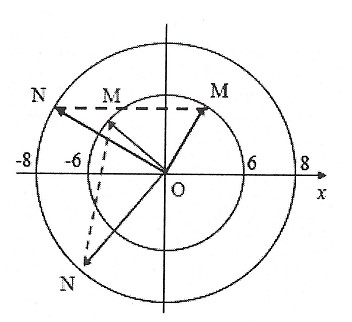
\includegraphics[scale=0.8]{../figs/VN12-PH-06-P-005-1-h1.jpg}
		\end{center}
		
		
		Khoảng cách giữa M và N là $\Delta x=\left| x_M-x_N \right|=\left|6\cos \left(\omega t+\varphi_1 \right)-  8\cos \left(\omega t+\varphi_2 \right) \right| =A\left|\cos \left( \omega t+\varphi \right)  \right|  $.
		
		Khoảng cách lớn nhất khi MN có phương nằm ngang, suy ra $6^2+8^2=10^2$, suy ra OM  luôn vuông góc với ON.
		
		Ở thời điểm mà M có động năng bằng thế năng tại: $x_M=A\dfrac{\sqrt{2}}{2}\left( W_\text{đM}= W_\text{tM}=\dfrac{1}{2}W_M \right) $.
		
		Tức OM hợp với Ox góc $\dfrac{\pi}{4}$, suy ra ON hợp với Ox góc $\dfrac{\pi}{4}$ hay  $x_N=-A\dfrac{\sqrt{2}}{2}$.
		
		Suy ra $W_\text{đN}=W_\text{tN}=\dfrac{1}{2}W_N$.
		
		Do đó, $\dfrac{W_\text{tM}}{W_\text{tN}}=\dfrac{W_\text{M}}{W_\text{N}}=\dfrac{9}{16}$.
		
		
	}
	\item \mkstar{3}
	
	\cauhoi{
		
		Hai chất điểm dao động điều hòa cùng tần số, trên hai đường thẳng song song với nhau và song song với trục Ox có phương trình lần lượt là $x_1=A_1\cos \left(\omega t+\varphi_1 \right)$   và $x_2=A_2\cos \left(\omega t+\varphi_2 \right)$. Giả sử $x=x_1+x_2$   và $y=x_1-x_2$. Biết rằng biên độ dao động của $x$ gấp $2$ lần biên độ dao động của $y$. Độ lệch pha giữa $x_1$ và $x_2$ là $\Delta \varphi$. Giá trị nhỏ nhất của  $\cos \Delta \varphi$ là
		\begin{mcq}(4)
			\item $\text{0,5}$.
			\item $\text{0,25}$.
			\item $-1$.
			\item $\text{0,6}$.
		\end{mcq}
	}
	\loigiai{
		\textbf{Đáp án D.}
		
		Ta có: $A_x^2=A_1^2+A_2^2+2A_1A_2\cos \Delta \varphi=4A_Y^2$ và $A_y^2=A_1^2+A_2^2-2A_1A_2\cos \Delta \varphi$.
		
		Suy ra: $4A_1A_2\cos \Delta \varphi =3A_y^2$ và $5A_y^2=2\left( A_1^2+A_2^2\right)$.
		
		Suy ra $\cos \Delta \varphi=\dfrac{3}{10}\cdot \dfrac{A_1^2+A_2^2}{A_1A_2}\geq \dfrac{3}{10} \cdot \dfrac{2A_1A_2}{A_1A_2}= \text{0,6}$.
		
		
	}
	\item \mkstar{3}

\cauhoi{
	
	Một chất điểm dao động điều hòa có đồ thi biểu diễn sự phụ thuộc của li độ $x$ vào thời gian $t$ như hình vẽ. Tại thời điểm $t = \text{0,2}\ \text{s}$, chất có li độ $2\ \text{cm}$. Ở thời điểm $t = \text{0,9}\ \text{s}$, gia tốc của chất điểm có giá trị bằng
	\begin{center}
		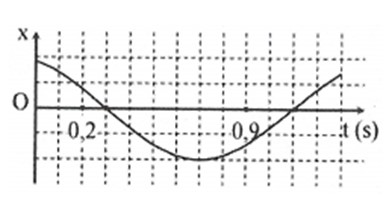
\includegraphics[scale=0.8]{../figs/VN12-PH-06-P-005-1-h7.jpg}
	\end{center}
	
	\begin{mcq}(4)
		\item $\text{14,5}\ \text{cm/s}^2$.
		\item $\text{57,0}\ \text{cm/s}^2$.
		\item $\text{5,7}\ \text{m/s}^2$.		
		\item $\text{1,45}\ \text{m/s}^2$.
	\end{mcq}
	
}
\loigiai{
	\textbf{Đáp án B.}
	
	Áp dụng công thức: 
	
	Dựa vào đồ thị ta thấy mỗi ô vuông ứng với thời gian là $\text{0,1}\ \text{s}$.
	
	Khoảng thời gian $2$ lần liên tiếp vật có li độ $x=0$ là (ứng với 8 ô)
	
	Tại thời điểm $t = \text{0,3}\ \text{s}$ ta có: $x=0\ \text{cm}, \ v<0$, suy ra $\varphi_3=\dfrac{\pi}{2}$.
	
	Pha dao động tại thời điểm $t = \text{0,2}\ \text{s}$ là $\varphi_2=\varphi_3-\dfrac{5\pi}{4}\cdot \text{0,1}=\dfrac{3\pi}{8}$.
	
	Do đó $A\cos \dfrac{3\pi}{8}=2\Rightarrow A=\text{5,226}\ \text{cm}$.
	
	Mặt khác $\Delta t=t_{0,2\rightarrow 0,9}=\text{0,7}\ \text{s}\Rightarrow \Delta \varphi=\text{0,7}\cdot \dfrac{5\pi}{4}=\dfrac{7\pi}{8}$.
	
	Do đó $x_{t=0,9}=A\cos \left(\dfrac{3\pi}{8}+\dfrac{7\pi}{8} \right)=-\text{3,696}\ \text{cm}\Rightarrow a=-\omega^2 x=57\ \text{cm/s}^2$.
	
}
\item \mkstar{3}

\cauhoi{
	
	Hình vẽ là đồ thị biểu diễn độ dời của dao động $x$ theo thời gian $t$ của một vật dao động điều hòa. Phương trình dao động của vật là
	\begin{center}
		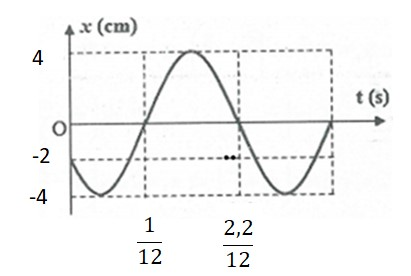
\includegraphics[scale=0.8]{../figs/VN12-PH-06-P-005-1-h6.jpg}
	\end{center}
	
	\begin{mcq}(2)
		\item $x=4\cos \left( 10\pi t+\dfrac{2\pi}{3}\right)\ \text{cm}$.
		\item  $x=4\cos \left( 20\pi t+\dfrac{2\pi}{3}\right)\ \text{cm}$.
		\item  $x=4\cos \left( 10\pi t+\dfrac{5\pi}{6}\right)\ \text{cm}$.	
		\item  $x=4\cos \left( 20\pi t-\dfrac{\pi}{3}\right)\ \text{cm}$.
	\end{mcq}
	
}
\loigiai{
	\textbf{Đáp án A.}
	
	Ta có  $A=4\ \text{cm}, \ \dfrac{T}{2}=\dfrac{\text{2,2}-1}{12}\Rightarrow T=\dfrac{1}{5}\ \text{s}\Rightarrow \omega =10\pi$.
	
	Tại thời điểm $t = 0$ ta có: $x=-2=-\dfrac{A}{2}, \ v<0$, suy ra $\varphi_0=\dfrac{2\pi}{3}$.
	
}

\item \mkstar{3}

\cauhoi{
	
	Đồ thị dao động của một chất điểm dao động điều hòa như hình vẽ. Phương trình biểu diễn sự phụ thuộc của vận tốc của vật theo thời gian là
	
	\begin{center}
		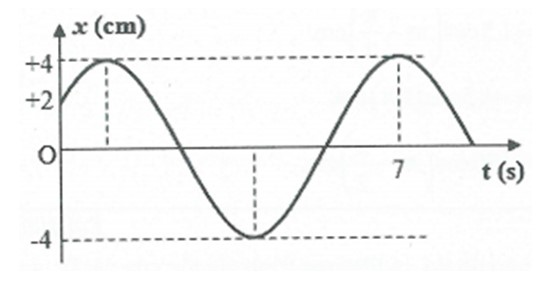
\includegraphics[scale=0.8]{../figs/VN12-PH-06-P-005-1-h8.jpg}
	\end{center}
	\begin{mcq}(2)
		\item $v=\dfrac{4\pi}{3} \cos \left( \dfrac{\pi}{3} t+\dfrac{\pi}{6}\right)\ \text{cm/s} $.
		\item $v=\dfrac{4\pi}{3} \cos \left( \dfrac{\pi}{6} t+\dfrac{5\pi}{6}\right)\ \text{cm/s} $.
		\item $v=4\pi \cos \left( \dfrac{\pi}{3} t+\dfrac{\pi}{3}\right)\ \text{cm/s} $.
		\item $v=4\pi \cos \left( \dfrac{\pi}{6} t+\dfrac{\pi}{3}\right)\ \text{cm/s} $.
	\end{mcq}
	
}
\loigiai{
	\textbf{Đáp án A.}
	
	Dựa vào đồ thị ta thấy: tại thời điểm $t=0$, suy ra $x=2, \ v>0\Rightarrow \varphi_0=-\dfrac{\pi}{3}$.
	
	Lại có: $t_{2 \rightarrow 4}+T=7\Rightarrow T=6\ \text{s}\Rightarrow \omega=\dfrac{\pi}{3}\ \text{rad/s}$.
	
	Do đó $x=4\cos \left( \dfrac{\pi t}{3}-\dfrac{\pi}{3}\right)\ \text{cm}\Rightarrow v=\dfrac{4\pi}{3}\cos \left( \dfrac{\pi t}{3}+\dfrac{\pi}{6}\right)\ \text{cm/s}$. 
	
	
	
}
\item \mkstar{3}

\cauhoi{
	
	Cho hai dao dộng cùng phương có phương trình $x_1=A_1\cos \left(\omega t+ \varphi_1 \right) $  và  $x_2=A_1\cos \left(\omega t + \varphi_2 \right) $  ($x$ tính bằng cm, $t$ được tính bằng s). Đồ thị dao động tổng hợp $x=x_1+x_2$ có dạng như hình vẽ. Cặp phương trình $x_1, \ x_2 $ nào sau đây thỏa mãn với đồ thị?
	\begin{center}
		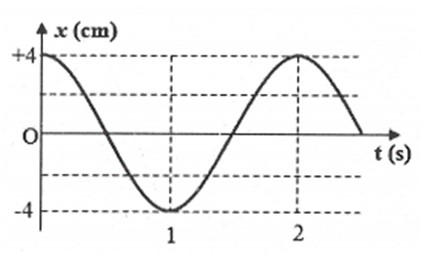
\includegraphics[scale=0.8]{../figs/VN12-PH-06-P-005-1-h9.jpg}
	\end{center}
	
	\begin{mcq}
		\item $x_1=2\sqrt{2}\cos \left( \pi t-\dfrac{\pi}{4}\right)\ \text{cm}$ và $x_2=2\sqrt{2}\cos \left( \pi t+\dfrac{\pi}{4}\right)\ \text{cm}$.
		\item $x_1=2\cos \left( \pi t-\dfrac{\pi}{2}\right)\ \text{cm}$ và $x_2=2\cos \left( \pi t+\dfrac{\pi}{2}\right)\ \text{cm}$.
		\item $x_1=6\cos \left( \pi t+\dfrac{\pi}{2}\right)\ \text{cm}$ và $x_2=2\cos \left( \pi t-\dfrac{\pi}{2}\right)\ \text{cm}$.
		\item $x_1=4\cos \left( \pi t+\dfrac{\pi}{3}\right)\ \text{cm}$ và $x_2=4\cos \left( \pi t-\dfrac{\pi}{3}\right)\ \text{cm}$.
	\end{mcq}
	
}
\loigiai{
	\textbf{Đáp án D.}
	
	Dựa vào đồ thị ta có: $A=4\ \text{cm}, \ \dfrac{T}{2}=1\ \text{s}\Rightarrow T=2\ \text{s}\Rightarrow \omega =\pi\ \text{rad/s}$.
	
	Tại thời điểm $t=0\Rightarrow x=A\Rightarrow \varphi=0$.
	
	Do đó  $x=x_1+x_2=4\cos \pi t=4\cos \left( \pi t+\dfrac{\pi}{3}\right)+ 4\cos \left( \pi t-\dfrac{\pi}{3}\right)$.
	
	
	
	
}

\item \mkstar{3}

\cauhoi{ 
	
	Một chất điểm dao động điều hòa dọc theo trục Ox, với O  trùng với vị trí cân bằng của chất điểm. Đường biểu diễn sự phụ thuộc li độ chất điểm theo thời gian $t$ cho ở hình vẽ. Phương trình vận tốc của chất điểm là
	\begin{center}
		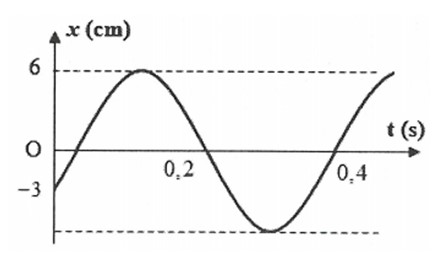
\includegraphics[scale=0.8]{../figs/VN12-PH-06-P-005-1-H5.jpg}
	\end{center}
	
	
	\begin{mcq}(2)
		\item $v=60\pi \cos \left( 5\pi t-\dfrac{\pi}{3}\right) $.
		\item $v=60\pi \cos \left( 5\pi t-\dfrac{\pi}{6}\right) $.
		\item $v=60\cos \left( 5\pi t-\dfrac{\pi}{3}\right) $.
		\item $v=60\pi \cos \left( 5\pi t-\dfrac{\pi}{6}\right) $.
	\end{mcq}
	
}
\loigiai{
	\textbf{Đáp án B.}
	
	
	
	Biên độ doa động của vật là $A = 6\ \text{cm}$.
	
	Dựa vào đồ thị ta thấy rằng sau $\text{0,2}\ \text{s}$ trạng thái dao động vật được lặp lại, do đó  $T=\text{0,2}\ \text{s}\Rightarrow  \omega=\dfrac{2\pi}{T}=5\pi \ \text{rad/s}$.
	
	Tại thời điểm bạn đầu $x=-3\ \text{cm}=-\dfrac{A}{2}$ và $v>0$, suy ra $\varphi_0=-\dfrac{2\pi}{3}$.
	
	
	Do đó phương trình dao động của vật là $x=6\cos \left(5\pi t-\dfrac{2\pi}{3}\right)\ \text{cm}$.
	
	Suy ra $v=60\pi \cos \left( 10\pi t-\dfrac{2\pi}{3}+\dfrac{\pi}{2}\right)= 60\pi \cos \left( 10\pi t-\dfrac{\pi}{6}\right) $.
	
	
	
	
	
}
	\item \mkstar{4}
	
	\cauhoi{
		
		Cho $D_1, \ D_2$ và $D_3$ là ba dao động điều hòa cùng phương, cùng tần số. Dao động tổng hợp của $D_1$   và $D_2$  có phương trình là $x_{12}=3\sqrt{3}\cos \left( \omega t+\dfrac{\pi}{2}\right) $  cm. Dao động tổng hợp của $D_2$   và $D_3$   có phương trình  $x_{23}=3\cos \left( \omega t\right) $  cm. Dao động $D_1$   ngược pha với dao động $D_3$. Biên độ dao động $D_2$  có giá trị nhỏ nhất là
		
		\begin{mcq}(4)
			\item $\text{2,6}\ \text{cm}$.
			\item $\text{2,7}\ \text{cm}$.
			\item $\text{3,6}\ \text{cm}$.
			\item $\text{3,7}\ \text{cm}$.
		\end{mcq}
	}
	\loigiai{
		\textbf{Đáp án A.}
		
		Ta có: $x_1+x_2=x_\text{12}=3\sqrt{3}\cos \left( \omega t+\dfrac{\pi}{2}\right)$   và  $x_{23}=x_2+x_3=3\cos \left( \omega t\right) $  cm.
		
		Suy ra $x_1-x_3=3\sqrt{3}\angle \dfrac{\pi}{2}-3\angle 0=6\angle \dfrac{2\pi}{3}$.
		
		Do dao động $D_1$ ngược pha với dao động $D_3$ nên   $x_3=-kx_1\Rightarrow x_1=\dfrac{6}{k+1}\angle \dfrac{2\pi}{3}$ với $k>0$.
		
		Do đó $x_2=3\sqrt{3}\angle \dfrac{\pi}{2}-\dfrac{6}{k+1}\angle \dfrac{2\pi}{3}\ (k>0) $.
		
		Suy ra $A_2^2=(3\sqrt{3})^2+\left( \dfrac{6}{k+1}\right)^2-2\cdot 3\sqrt{3}\cdot \dfrac{6}{k+1}\cdot \cos \dfrac{\pi}{6}=27+t^2-9t\ (t=\dfrac{6}{k+1}) $.
		
		Vậy $A_2^2=\left(t-\dfrac{9}{2} \right)^2+\dfrac{27}{4}\geq \dfrac{27}{4}\Rightarrow A_2\geq \dfrac{3\sqrt{3}}{2}=\text{2,6}\ \text{cm} $.
		
		Dấu bằng xảy ra khi $\dfrac{6}{k+1}=\dfrac{9}{2}\Rightarrow k=\dfrac{1}{3}\ \text{thỏa mãn}$. 
		
		
	}
	\item \mkstar{4}
	
	\cauhoi{ 
		
		Điểm sáng A đặt trên trục chính của một thấu kính, cách thấu kính $10\ \text{cm}$. Chọn trục tọa độ Ox vuông góc với trục chính, gốc O nằm trên trục chính của thấu kính. Cho A dao động điều hòa theo phương của trục Ox. Biết phương trình dao động của A là $x$ và ảnh $A'$  là $x'$  của nó qua thấu kính được biểu diễn như hình vẽ. Thời điểm lần thứ $2018$ mà khoảng cách giữa vật sáng và ảnh của nó khi điểm sáng A dao động là $5\sqrt{5}\ \text{cm}$ có giá trị gần bằng giá trị nào sau đây nhất?
		\begin{center}
			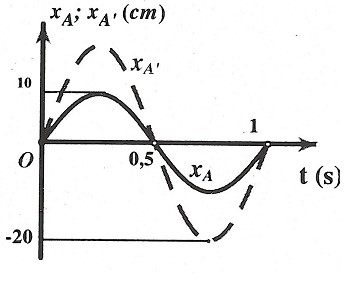
\includegraphics[scale=0.8]{../figs/VN12-PH-06-P-005-1-h2.jpg}
		\end{center}	
		\begin{mcq}(4)
			\item $\text{504,6}\ \text{s}$.
			\item $\text{506,8}\ \text{s}$.
			\item $\text{506,4}\ \text{s}$.
			\item $\text{504,2}\ \text{s}$.
		\end{mcq}
	}
	\loigiai{
		\textbf{Đáp án D.}
		
		\begin{center}
			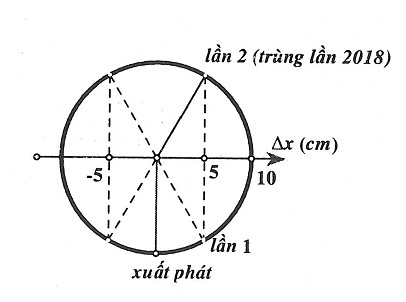
\includegraphics[scale=0.8]{../figs/VN12-PH-06-P-005-1-h3.jpg}
		\end{center}
		
		Từ đồ thị ta được: ảnh nhỏ hơn vật và cùng tính chất với vật, suy ra đây là thấu kính hội tụ,  $k = 2$.
		
		Áp dụng $k=\dfrac{f}{f-d}\Rightarrow f=20\ \text{cm}$, suy ra $d'=\dfrac{df}{d-f}=-20\ \text{cm}$.
		
		Khoảng cách vật và ảnh: $\Delta d=|d+d'|=10\ \text{cm}$.
		
		Từ đồ thị ta cũng viết được: $x_A=10\cos \left(\omega t-\dfrac{\pi}{2} \right) \ \text{cm} $ và $x_A'=20\cos \left(\omega t-\dfrac{\pi}{2} \right)\ \text{cm}$.
		
		Phương trình khoảng cách ảnh và vật trên phương Ox:
		$\Delta x=x_A-x_A'=10\cos \left( \omega t -\dfrac{\pi}{2}\right)\ \text{cm} $.
		
		
		Suy ra, khoảng cách trực tiếp giữa vật và ảnh: $X=\sqrt{\Delta x^2+\Delta d^2}$  hay $X^2=\Delta x^2+100$.
		
		Khi $X=5\sqrt{5}\ \text{cm}$, suy ra $|\Delta x|=5\ \text{cm}$.
		
		Thời gian qua lần thứ $2018$ thỏa $t=505T+t_2$ (thời gian lần thứ $2$ tính từ lúc $t = 0$).
		
		Hay $t=504T+\dfrac{T}{4}+\dfrac{T}{6}=\text{504,2}\ \text{s}$. 
		
		
	}
	\item \mkstar{4}
	
	\cauhoi{
		
		Hai vật $(1)$ và vật $(2)$ có cùng khối lượng $m$, nằm trên mặt phẳng nằm ngang và mỗi vật được nối với tường bằng mỗi lò xo có độ cứng khác nhau thỏa mãn $k_2=4k_1$. Vật $(1)$ lúc đầu nằm ở $\text{O}_1$, vật $(2)$ lúc đầu nằm ở $\text{O}_2$, biết $\text{O}_1\text{O}_2=12\ \text{cm}$. Nén đồng thời lò xo $(1)$ một đoạn $10\ \text{cm}$, lò xo $(2)$ một đoạn $5\ \text{cm}$ rồi thả nhẹ cho hai vật dao động. Trong quá trình dao động khoảng cách ngắn nhất của hai vật gần giá trị nào nhất trong các giá trị nào sau đây?
		\begin{center}
			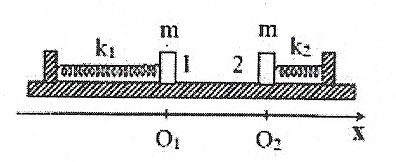
\includegraphics[scale=0.8]{../figs/VN12-PH-06-P-005-1-h4.jpg}
		\end{center}
		\begin{mcq}(4)
			\item $5\ \text{s}$.
			\item $7\ \text{s}$.
			\item $3\ \text{s}$.			
			\item $6\ \text{s}$.
		\end{mcq}
		
	}
	\loigiai{
		\textbf{Đáp án A.}
		
		
		Biên độ dao động của các vật là: $A_1=10\ \text{cm}, \ A_2=5\ \text{cm}$.
		
		Khoảng cách lúc đầu của hai vật là $\text{O}_1\text{O}_2=12\ \text{cm}$.
		
		Chọn gốc thời gian là lúc vật bắt đầu chuyển động, chọn gốc tọa độ là vị trí  $\text{O}_1$, chiều dương là chiều chuyển động của vật $(2)$.
		
		Phương trình dao động của các vật là: $x_1=10\cos \left( \omega t+\pi\right)=-10\cos \left( \omega t\right)$ và $x_2=12+ 5\cos \left( 2\omega t\right) $. 
		
		Khoảng cách giữa hai vật là:  $\Delta x=|x_2-x_1|=|12+5\cos \left( 2\omega t\right) +10\cos \left( \omega t\right)(1)|$.
		
		Sử dụng công thức lượng giác $\cos 2\alpha=2\cos^2 \alpha-1$  vào $(1)$, ta có được $\Delta x=|10\cos^2\left( \omega t\right)+10\cos\left( \omega t\right) +7 |$   
		
		Đây là một phương trình bậc hai theo ẩn $\cos\left( \omega t\right)$. Do đó $\Delta x_\text{min}=-\dfrac{\Delta }{4a}=\text{4,5}\ \text{cm}$  gần với đáp án A nhất. 
	}

\end{enumerate}
\loigiai{\textbf{Đáp án}
	\begin{center}
		\begin{tabular}{|m{2.8em}|m{2.8em}|m{2.8em}|m{2.8em}|m{2.8em}|m{2.8em}|m{2.8em}|m{2.8em}|m{2.8em}|m{2.8em}|}
			\hline
			1. B & 2. A & 3. B & 4. D & 5. A & 6. C & 7. C & 8. A & 9. A & 10. C \\
			\hline
			11. B & 12. D & 13. B & 14. A & 15. A & 16. D & 17. B & 18. A & 19. D & 20. A\\
			\hline
		\end{tabular}
\end{center}}
\stopcontents[mychapters]
\chapter{Ôn tập: Chương I. Dao động cơ}
	\begin{enumerate}[label=\bfseries Câu \arabic*:]
	\item \mkstar{1}
	
	\cauhoi{
		Trong dao động điều hòa của một vật thì tập hợp ba đại lượng nào sau đây không đổi theo thời gian?
		
		\begin{mcq}(2)
			\item Biên độ, tần số, cơ năng.
			\item Biên độ, tần số, gia tốc.
			\item Động năng, tần số, lực hồi phục.
			\item Lực hồi phục, vận tốc, cơ năng.
		\end{mcq}
	}
	\loigiai{
		\textbf{Đáp án A.}
		
		Tập hợp ba đại lượng không đổi theo thời gian: biên độ, tần số, cơ năng.
	}

	\item \mkstar{1}

\cauhoi{
	
	Trong dao động điều hòa, những đại lượng dao động cùng tần số với li độ là
	\begin{mcq}(2)
		\item động năng, thế năng và lực kéo về.
		\item vận tốc, gia tốc và lực kéo về.
		\item vận tốc, động năng và thế năng.
		\item vận tốc, gia tốc và động năng.
	\end{mcq}
}
\loigiai{
	\textbf{Đáp án B.}
	
	Trong dao động điều hòa, những đại lượng cùng tần số với li độ là: vận tốc, gia tốc, lực kéo về.
	
	Những đại lượng dao động khác tần số với li độ (cụ thể là $f'=2f$) là: động năng, thế năng.
}

	\item \mkstar{1}

\cauhoi{
	Phát biểu nào sau đây \textbf{không} đúng về dao động điều hòa?
	
	\begin{mcq}
		\item Hợp lực tác dụng vào vật có giá trị lớn nhất khi vật đi qua vị trí cân bằng.
		\item Động năng của vật biến đổi tuần hoàn với chu kì bằng một nửa chu kì dao động của vật.
		\item Tốc độ của vật lớn nhất khi vật đi qua vị trí cân bằng.
		\item Vận tốc của vật lệch pha $\xsi{0,5\pi}{rad}$ so với li độ dao động.
	\end{mcq}
}
\loigiai{
	\textbf{Đáp án A.}
	
	Dựa vào định luật II Niu-tơn:
	$$\Sigma \vec{F} = m \vec{a}.$$
	
	Tại vị trí cân bằng thì $a=0$, suy ra $\Sigma \vec{F} = 0$. Vậy hợp lực tác dụng vào vật bằng 0 khi vật đi qua vị trí cân bằng.
}

	\item \mkstar{1}

\cauhoi{
	
	Hiện tượng cộng hưởng cơ học diễn ra khi nào?
	\begin{mcq}
		\item Tần số dao động cưỡng bức bằng tần số dao động riêng của hệ.
		\item Tần số của lực cưỡng bức bé hơn tần số riêng của hệ.
		\item Tần số của lực cưỡng bức bằng tần số của dao động cưỡng bức.
		\item Tần số của lực cưỡng bức lớn hơn tần số riêng của hệ.
	\end{mcq}
}
\loigiai{
	\textbf{Đáp án A.}
	
	Hiện tượng cộng hưởng cơ học diễn ra khi tần số dao động cưỡng bức bằng tần số dao động riêng của hệ.
}

	\item \mkstar{1}

\cauhoi{
	Khi quả nặng của một con lắc đơn đi từ vị trí cân bằng đến vị trí biên thì nhận định nào dưới đây \textbf{sai}?
	
	\begin{mcq}(2)
		\item Li độ góc tăng dần.
		\item Gia tốc tăng dần.
		\item Tốc độ giảm dần.
		\item Lực căng dây tăng dần.
	\end{mcq}
}
\loigiai{
	\textbf{Đáp án D.}
	
	Khi quả nặng của một con lắc đơn đi từ vị trí cân bằng đến vị trí biên thì lực căng dây giảm.
}

	\item \mkstar{1}

\cauhoi{
	Trong dao động điều hòa, gọi $\omega$ là tần số góc, $A$ là biên độ dao động. Công thức liên hệ giữa $v$ và $x$ nào dưới đây là đúng?
	
	\begin{mcq}(2)
		\item $x^2 = \dfrac{v^2}{\omega^2} + A^2$.
		\item $\dfrac{v^2}{\omega^2} = A^2 - x^2$.
		\item $x^2 = \dfrac{\omega^2}{v^2} + A^2$.
		\item $A^2 = \dfrac{\omega^2}{v^2} + x^2$.
	\end{mcq}
}
\loigiai{
	\textbf{Đáp án B.}
	
	$$A^2 = x^2 + \dfrac{v^2}{\omega^2} \Rightarrow A^2 - x^2 = \dfrac{v^2}{\omega^2}.$$
}

	\item \mkstar{2}

\cauhoi{
	Một chất điểm dao động điều hòa theo phương trình $x=5 \cos (2\pi t + \pi)\ \text{cm}$. Quãng đường vật đi được sau $\SI{2}{s}$ là
	
	\begin{mcq}(4)
		\item $\SI{20}{cm}$.
		\item $\SI{10}{cm}$.
		\item $\SI{40}{cm}$.
		\item $\SI{80}{cm}$.
	\end{mcq}
}
\loigiai{
	\textbf{Đáp án C.}
	
	Chu kì dao động:
	$$T=\dfrac{2\pi}{\omega} = \SI{1}{s}.$$
	
	Vì $t=\SI{2}{s}=2T$ nên quãng đường vật đi được là
	$$S=2\cdot 4A = 2 \cdot 4 \cdot \SI{5}{cm} = \SI{40}{cm}.$$
}

	\item \mkstar{2}

\cauhoi{
	Một vật dao động điều hòa có biểu thức của gia tốc là $a=-100\pi^2 \cos (100 \pi t - \pi /2)\ \text{cm/s}^2$. Quãng đường vật đi được trong 1 chu kì dao động là
	
	\begin{mcq}(4)
		\item $\SI{1}{cm}$.
		\item $\SI{4}{cm}$.
		\item $\xsi{400\pi ^2}{cm}$.
		\item $\xsi{4\pi^2}{cm}$.
	\end{mcq}
}
\loigiai{
	\textbf{Đáp án B.}
	
	Dựa vào mối liên hệ giữa gia tốc cực đại và biên độ dao động, ta được:
	$$a_\text{max} = -\omega^2 A \Rightarrow A = \dfrac{-a_\text{max}}{\omega^2} = \SI{1}{cm}.$$
	
	Quãng đường vật đi được trong 1 chu kì:
	$$S=4A = \SI{4}{cm}.$$
}

	\item \mkstar{2}

\cauhoi{
	Đồ thị vận tốc-thời gian của một vật dao động điều hòa được cho như hình vẽ.
	\begin{center}
		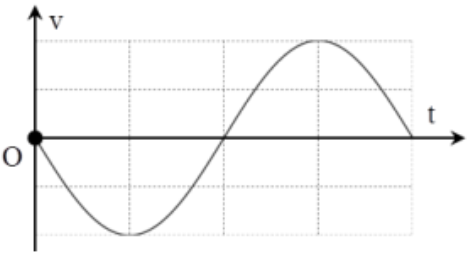
\includegraphics[scale=0.8]{../figs/VN12-2021-PH-TP007-1}
	\end{center}

	Mốc thời gian đã được chọn vào lúc
	\begin{mcq}
		\item vật đi qua vị trí cân bằng theo chiều âm.
		\item vật đi qua vị trí cân bằng theo chiều dương.
		\item vật ở biên âm.
		\item vật ở biên dương.
	\end{mcq}
}
\loigiai{
	\textbf{Đáp án D.}
	
	Dựa vào đồ thị, tại thời điểm $t=0$ thì $v=0$ và có xu hướng về phía vận tốc âm. Đó là thời điểm mà vật ở vị trí biên dương.
}

	\item \mkstar{2}

\cauhoi{
	Khoảng thời gian liên tiếp để động năng và thế năng của một vật dao động điều hòa bằng nhau là $\SI{0.3}{s}$. Chu kì dao động của vật là
	
	\begin{mcq}(4)
		\item $\SI{0.3}{s}$.
		\item $\SI{0.6}{s}$.
		\item $\SI{0.9}{s}$.
		\item $\SI{1.2}{s}$.
	\end{mcq}
}
\loigiai{
	\textbf{Đáp án D.}
	
	Khoảng thời gian liên tiếp giữa hai lần động năng bằng thế năng là $T/4$:
	$$\dfrac{T}{4} = \SI{0.3}{s} \Rightarrow T = \SI{1.2}{s}.$$
}

	\item \mkstar{2}

\cauhoi{
	Một vật dao động điều hòa với biên độ $A$ và cơ năng $W$. Chọn mốc thế năng tại vị trí cân bằng. Khi vật đi qua vị trí có li độ $x=2A/3$ thì động năng của vật là
	
	\begin{mcq}(4)
		\item $\dfrac{5}{9}W$.
		\item $\dfrac{4}{9} W$.
		\item $\dfrac{7}{9} W$.
		\item $\dfrac{2}{9} W$.
	\end{mcq}
}
\loigiai{
	\textbf{Đáp án A.}
	
	Lập tỉ lệ:
	$$\dfrac{W_\text{đ}}{W} = \dfrac{A^2 - x^2}{A^2} = \dfrac{5}{9}.$$
}

	\item \mkstar{2}

\cauhoi{
	Tiến hành thí nghiệm đo gia tốc trọng trường $g$ bằng con lắc đơn, một học sinh đo được chiều dài con lắc là $l = \bar{l} \pm \Delta l$ (đơn vị m). Chu kì dao động nhỏ của nó là $T=\bar{T} \pm \Delta T$ (đơn vị s). Bỏ qua sai số của $\pi$, biểu thức sai số của $g$ là
	
	\begin{mcq}(2)
		\item $\dfrac{\Delta g}{\bar{g}} = \dfrac{\Delta T}{\bar{T}} + \dfrac{2 \Delta l}{\bar{l}}$.
		\item $\dfrac{\Delta g}{\bar{g}} = \dfrac{\Delta T}{\bar{T}} + \dfrac{\Delta l}{\bar{l}}$.
		\item $\dfrac{\Delta g}{\bar{g}} = \dfrac{2\Delta T}{\bar{T}} + \dfrac{2 \Delta l}{\bar{l}}$.
		\item $\dfrac{\Delta g}{\bar{g}} = \dfrac{2\Delta T}{\bar{T}} + \dfrac{\Delta l}{\bar{l}}$.
	\end{mcq}
}
\loigiai{
	\textbf{Đáp án D.}
	
	Biểu thức xác định $g$:
	$$g=\left(\dfrac{2\pi}{T}\right)^2 l \Rightarrow \dfrac{\Delta g}{\bar{g}} = \dfrac{2\Delta T}{\bar{T}} + \dfrac{\Delta l}{\bar{l}}$$
}

	\item \mkstar{2}

\cauhoi{
	Một vật nhỏ khối lượng $\SI{100}{g}$ dao động điều hòa trên một quỹ đạo thẳng dài $\SI{20}{cm}$ với tần số góc $\SI{6}{rad/s}$. Cơ năng của vật này là
	
	\begin{mcq}(4)
		\item $\SI{0.036}{J}$.
		\item $\SI{0.018}{J}$.
		\item $\SI{18}{J}$.
		\item $\SI{36}{J}$.
	\end{mcq}
}
\loigiai{
	\textbf{Đáp án B.}
	
	Tính biên độ dao động dựa vào chiều dài quỹ đạo:
	$$A=\dfrac{L}{2} = \SI{10}{cm}.$$
	
	Cơ năng của vật:
	$$W=\dfrac{1}{2} m \omega^2 A^2 = \SI{0.018}{J}.$$
}

	\item \mkstar{2}

\cauhoi{
	Một vật nhỏ khối lượng $m=\SI{0.01}{kg}$ treo ở đầu một lò xo có độ cứng $k=\SI{4}{N/m}$, dao động điều hòa quanh vị trí cân bằng. Chu kì dao động của vật là
	
	\begin{mcq}(4)
		\item $\SI{0.624}{s}$.
		\item $\SI{0.314}{s}$.
		\item $\SI{0.196}{s}$.
		\item $\SI{0.157}{s}$.
	\end{mcq}
}
\loigiai{
	\textbf{Đáp án B.}
	
	Chu kì dao động:
	$$T=2\pi \sqrt{\dfrac{m}{k}} = \SI{0.0314}{s}.$$
}

	\item \mkstar{2}

\cauhoi{
	Một vật nặng treo vào đầu lò xo làm cho lò xo dãn ra $\SI{4}{cm}$, đầu kia treo vào một điểm O cố định. Hệ dao động điều hòa theo phương thẳng đứng. Cho $g=\xsi{\pi^2}{m/s^2}$. Chu kì dao động của hệ là
	
	\begin{mcq}(4)
		\item $\SI{0.8}{s}$.
		\item $\SI{0.4}{s}$.
		\item $\SI{0.2}{s}$.
		\item $\SI{1.6}{s}$.
	\end{mcq}
}
\loigiai{
	\textbf{Đáp án B.}
	
	Chu kì của dao động là
	$$T=2\pi \sqrt{\dfrac{\Delta l}{g}} = \SI{0.4}{s}.$$
}

	\item \mkstar{2}

\cauhoi{
	Một con lắc lò xo gồm lò xo có độ cứng $k=\SI{100}{N/m}$ và vật nặng có khối lượng $m$, dao động điều hòa quanh trục O$x$ nằm ngang. Thế năng của con lắc khi vật đi qua vị trí có li độ $x=\SI{3}{cm}$ theo chiều âm là
	
	\begin{mcq}(4)
		\item $\SI{0.045}{J}$.
		\item $\SI{0.09}{J}$.
		\item $\SI{-0.045}{J}$.
		\item $\SI{-0.09}{J}$.
	\end{mcq}
}
\loigiai{
	\textbf{Đáp án A.}
	
	Thế năng của con lắc khi vật ở vị trí $x=\SI{3}{cm}$:
	$$W_\text{t} = \dfrac{1}{2} kx^2 = \SI{0.045}{J}.$$
}

	\item \mkstar{2}

\cauhoi{
	Một con lắc lò xo dao động điều hòa với biên độ $A=\SI{10.0}{cm}$ và cơ năng $\SI{0.8}{J}$. Độ cứng của lò xo là
	
	\begin{mcq}(4)
		\item $\SI{80}{N/m}$.
		\item $\SI{40}{N/m}$.
		\item $\SI{1.6}{N/m}$.
		\item $\SI{160}{N/m}$.
	\end{mcq}
}
\loigiai{
	\textbf{Đáp án D.}
	
	Áp dụng biểu thức của cơ năng:
	$$W=\dfrac{1}{2} kA^2 \Rightarrow k = \SI{160}{N/m}.$$
}

	\item \mkstar{2}

\cauhoi{
	Một vật tham gia đồng thời hai dao động điều hòa cùng phương có phương trình lần lượt là $x_1=3\cos \left(10 \pi t + \dfrac{\pi}{6}\right)\ \text{cm}$ và $x_2 = 7 \cos \left(10 \pi t + \dfrac{13\pi}{6}\right)\ \text{cm}$. Dao động tổng hợp có phương trình là
	
	\begin{mcq}(2)
		\item $x=10 \cos \left(10 \pi t + \dfrac{7\pi}{3}\right)\ \text{cm}$.
		\item $x=4 \cos \left(10 \pi t + \dfrac{\pi}{6}\right)\ \text{cm}$.
		\item $x=10 \cos \left(20 \pi t + \dfrac{\pi}{6}\right)\ \text{cm}$.
		\item $x=10 \cos \left(10 \pi t + \dfrac{\pi}{6}\right)\ \text{cm}$.
	\end{mcq}
}
\loigiai{
	\textbf{Đáp án D.}
	
	Phương trình dao động tổng hợp:
	$$x=10 \cos \left(10 \pi t + \dfrac{\pi}{6}\right)\ \text{cm}$$
}

	\item \mkstar{2}

\cauhoi{
	Một con lắc lò xo có độ cứng $k$ treo thẳng đứng, đầu trên gắn cố định, đầu dưới treo quả cầu nhỏ ở nơi có gia tốc trọng trường $g$. Khi vật ở vị trí cân bằng, lò xo có độ dãn $\Delta l$. Cho con lắc dao động điều hòa theo phương thẳng đứng với biên độ $A$ (với $A> \Delta l$). Lực đàn hồi cực tiểu của lò xo được xác định bởi biểu thức nào sau đây?
	
	\begin{mcq}(2)
		\item $F_\text{đh min} = k A$.
		\item $F_\text{đh min} = k(A - \Delta l)$.
		\item $F_\text{đh min} = 0$.
		\item $F_\text{đh min} = k (\Delta l - A)$.
	\end{mcq}
}
\loigiai{
	\textbf{Đáp án C.}
	
	Khi $A<\Delta l$ thì $F_\text{đh min} = k (\Delta l - A)$.
	
	Khi $A>\Delta l$ thì $F_\text{đh min} = 0$.
}

	\item \mkstar{3}

\cauhoi{
	Tỉ số giữa gia tốc của một vật dao động điều hòa so với gia tốc cực đại tại vị trí động năng gấp 2 lần thế năng là
	
	\begin{mcq}(4)
		\item $\dfrac{1}{2}$.
		\item $\dfrac{1}{\sqrt{2}}$.
		\item $\dfrac{1}{3}$.
		\item $\dfrac{1}{\sqrt{3}}$.
	\end{mcq}
}
\loigiai{
	\textbf{Đáp án D.}
	
	Ta có tỉ số:
	$$\dfrac{W_\text{đ}}{W_\text{t}} = 2 \Rightarrow \dfrac{A^2 - x^2}{x^2} = 2 \Rightarrow |x| = \dfrac{A}{\sqrt{3}} \Rightarrow a = \dfrac{a_\text{max}}{\sqrt{3}}.$$
}

	\item \mkstar{3}

\cauhoi{
	Một vật dao động điều hòa theo phương trình $x=2 \cos (\pi t - \pi /3)\ \text{cm}$, trong đó $t$ tính bằng giây. Tính từ lúc $t=0$, thời điểm vật đi qua vị trí có thế năng bằng 3 lần động năng lần thứ 2018 là
	
	\begin{mcq}(4)
		\item $\SI{1008.5}{s}$.
		\item $\SI{1009.5}{s}$.
		\item $\SI{1008}{s}$.
		\item $\SI{1009}{s}$.
	\end{mcq}
}
\loigiai{
	\textbf{Đáp án A.}
	
	Tại thời điểm $t=0$, vật ở vị trí $x=A \cos (-\dfrac{\pi}{3}) = \dfrac{A}{2}$, theo chiều dương.
	
	Vị trí mà vật có thế năng gấp 3 lần động nặng là $x=\dfrac{A\sqrt{3}}{2}$.
	
	Ta nhận thấy 2016 chia hết cho 4 (vì 1 chu kì có 4 lần thế năng gấp 3 lần động năng), nên ta phân tích lần thứ 2018 thành $2+2016$, nghĩa là phân tích thành 2 lần đầu và 2016 lần sau.
	
	Lần thứ nhất mà vật có thế năng gấp 3 lần động năng là thời điểm:
	$$t_1 = \dfrac{T}{6} - \dfrac{T}{12} = \dfrac{T}{12}.$$
	
	Lần thứ hai mà vật có thế năng gấp 3 lần động năng là thời điểm:
	$$t_2 = t_1 + 2 \cdot \dfrac{T}{12} = \dfrac{3T}{12}.$$
	
	Lần thứ 2018 mà vật có thế năng gấp 3 lần động năng là thời điểm:
	$$t_{2018} = t_2 + \dfrac{2016}{4} T = \dfrac{3T}{12} + 504T = \SI{1008.5}{s}.$$
	}

	\item \mkstar{3}

\cauhoi{
	Một chất điểm dao động điều hòa trên trục O$x$ với biên độ $\SI{10}{cm}$, chu kì $\SI{2}{s}$. Mốc thế năng ở VTCB. Tốc độ trung bình của chất điểm trong khoảng thời gian ngắn nhất khi chất điểm đi từ vị trí có động năng bằng 3 lần thế năng đến vị trí có động năng bằng $1/3$ lần thế năng là
	
	\begin{mcq}(4)
		\item $\SI{7.32}{cm/s}$.
		\item $\SI{21.96}{cm/s}$.
		\item $\SI{14.64}{cm/s}$.
		\item $\SI{26.12}{cm/s}$.
	\end{mcq}
}
\loigiai{
	\textbf{Đáp án B.}
	
	Quãng đường vật đi được:
	$$S=\dfrac{A\sqrt{3}}{2} - \dfrac{A}{2} = \xsi{-5+5\sqrt{3}}{cm}.$$
	
	Thời gian để đi hết quãng đường đó:
	$$t=\dfrac{T}{6} - \dfrac{T}{12} = \dfrac{T}{12} = \xsi{\dfrac{1}{6}}{s}.$$
	
	Vận tốc trung bình:
	$$v=\dfrac{S}{t} = \SI{21.96}{cm/s}$$
}

	\item \mkstar{3}

\cauhoi{
	Một vật nhỏ dao động điều hòa dọc theo trục O$x$. Khi vật cách vị trí cân bằng một đoạn $\SI{2}{cm}$ thì động năng của vật là $\SI{0.48}{J}$. Khi vật cách vị trí cân bằng một đoạn $\SI{6}{cm}$ thì động năng của vật là $\SI{0.32}{J}$. Biên độ dao động của vật bằng
	
	\begin{mcq}(4)
		\item $\SI{8}{cm}$.
		\item $\SI{14}{cm}$.
		\item $\SI{10}{cm}$.
		\item $\SI{12}{cm}$.
	\end{mcq}
}
\loigiai{
	\textbf{Đáp án B.}
	
	Vì cơ năng không đổi theo thời gian nên ta có:
	$$W_1 = W_2 \Rightarrow W_\text{đ1} + W_\text{t1} = W_\text{đ2} + W_\text{t2} \Rightarrow \dfrac{1}{2} m\omega^2 x_1^2 + \SI{0.48}{J} = \dfrac{1}{2} m \omega^2 x_2^2 + \SI{0.32}{J} \Rightarrow m \omega^2 = 100.$$
	
	Tính được cơ năng của vật:
	$$W=\dfrac{1}{2} m \omega^2 x_1^2 + W_\text{đ1} = \SI{0.5}{J}.$$
	
	Suy ra biên độ dao động là
	$$A=\sqrt{\dfrac{W}{\dfrac{1}{2} m \omega^2}} = \SI{10}{cm}.$$
}

	\item \mkstar{3}

\cauhoi{
	Một vật dao động điều hòa với tần số $f=\SI{3}{Hz}$. Tại thời điểm $t=\SI{1.5}{s}$, vật có li độ $x=\SI{4}{cm}$ và vận tốc $v=\xsi{24\pi \sqrt{3}}{cm/s}$ đang hướng về vị trí cân bằng. Phương trình dao động của vật là
	
	\begin{mcq}(2)
		\item $x= 8 \cos \left(6 \pi t - \dfrac{2\pi}{3}\right)\ \text{cm}$.
		\item $x= 8 \cos \left(6 \pi t - \dfrac{\pi}{3}\right)\ \text{cm}$.
		\item $x= 4\sqrt{3} \cos \left(6 \pi t + \dfrac{2\pi}{3}\right)\ \text{cm}$.
		\item $x= 4\sqrt{3} \cos \left(6 \pi t - \dfrac{\pi}{3}\right)\ \text{cm}$.
	\end{mcq}
}
\loigiai{
	\textbf{Đáp án A.}
	
	Tần số góc của dao động:
	$$\omega = 2\pi f = \xsi{6\pi}{rad/s}.$$
	
	Áp dụng hệ thức độc lập để xác định biên độ:
	$$A=\sqrt{x^2 + \dfrac{v^2}{\omega^2}} = \SI{8}{cm}.$$
	
	Khi đó, $x=\dfrac{A}{2}$ và vật đang hướng về vị trí cân bằng, nên pha của dao động là $\varphi_2 = \dfrac{\pi}{3}\ \text{rad}$.
	
	Trước đó $\SI{1.5}{s}=\SI{4.5}{} T$ chính là thời điểm ban đầu, tìm được pha ban đầu là
	$$\varphi = \dfrac{\pi}{3}\ \text{rad}-\xsi{9\pi}{rad} = \dfrac{-26\pi}{3}\ \text{rad}=\dfrac{-2\pi}{3}\ \text{rad}.$$
	
	Vậy phương trình dao động là $x=8 \cos \left(6\pi t - \dfrac{2\pi}{3}\right)\ \text{cm}$.
}

	\item \mkstar{3}

\cauhoi{
	Một con lắc lò xo gồm một quả cầu nhỏ gắn vào đầu một lò xo, dao động điều hòa với biên độ $\SI{2.5}{cm}$ dọc theo trục O$x$, với chu kì $\SI{1.2}{s}$. Vào thời điểm $t=0$, quả cầu đi qua vị trí cân bằng theo chiều dương của trục O$x$. Hỏi vào thời điểm nào sau đây quả cầu có li độ $x=\SI{1.25}{cm}$?
	
	\begin{mcq}(4)
		\item $t=\SI{0.04}{s}$.
		\item $t=\SI{0.75}{s}$.
		\item $t=\SI{0.5}{s}$.
		\item $t=\SI{0.6}{s}$.
	\end{mcq}
}
\loigiai{
	\textbf{Đáp án C.}
	
	Tần số góc của dao động:
	$$\omega = \dfrac{2\pi}{T} = \xsi{\dfrac{5\pi}{3}}{rad/s}.$$
	
	Pha ban đầu: $\varphi = \xsi{\dfrac{-\pi}{2}}{rad}$.
	
	Phương trình dao động:
	$$x=\SI{2.5}{} \cos \left(\dfrac{5\pi}{3} t - \dfrac{\pi}{2}\right)\ \text{cm}.$$
	
	Với $x=\SI{1.25}{cm}$ thì $t=\SI{0.5}{s}$.
}

	\item \mkstar{3}

\cauhoi{
	Một đầu của một lò xo được treo vào điểm cố định O, đầu kia treo một quả nặng $m_1$ thì vật dao động với chu kì $T_1 = \SI{0.6}{s}$. Khi thay vật $m_1$ thành vật $m_2$ thì vật dao động với chu kì $T_2=\SI{0.8}{s}$. Chu kì dao động khi treo đồng thời $m_1$ và $m_2$ vào lò xo là
	
	\begin{mcq}(4)
		\item $T=\SI{1.6}{s}$.
		\item $T=\SI{1.4}{s}$.
		\item $T=\SI{1.0}{s}$.
		\item $T=\SI{1.2}{s}$.
	\end{mcq}
}
\loigiai{
	\textbf{Đáp án C.}
	
	Ta có công thức tính chu kì:
	$$T=2\pi \sqrt{\dfrac{m}{k}} \Rightarrow m \sim T^2.$$
	
	Chu kì khi treo đồng thời $m_1$ và $m_2$:
	$$T^2 = T_1^2 + T_2^2 \Rightarrow T=\SI{1.0}{s}.$$
}

	\item \mkstar{3}

\cauhoi{
	Một chất điểm dao động điều hòa trên trục O$x$. Trong thời gian $\SI{31.4}{s}$ chất điểm thực hiện được 100 dao động toàn phần. Gốc thời gian là lúc chất điểm đi qua vị trí có li độ $\SI{2}{cm}$ theo chiều âm với tốc độ là $\xsi{40\sqrt{3}}{cm/s^2}$. Lấy $\pi = \SI{3.14}{}$. Phương trình dao động của chất điểm là
	
	\begin{mcq}(2)
		\item $x= 6 \cos \left(20 t - \dfrac{\pi}{6}\right)\ \text{cm}$.
		\item $x=4 \cos \left(20 t + \dfrac{\pi}{3}\right)\ \text{cm}$.
		\item $x= 4\cos \left(20 t - \dfrac{\pi}{3}\right)\ \text{cm}$.
		\item $x=6 \cos \left(20 t + \dfrac{\pi}{6}\right)\ \text{cm}$.
	\end{mcq}
}
\loigiai{
	\textbf{Đáp án B.}
	
	Ta có:
	$$T=\dfrac{\Delta t}{n} = \SI{0.314}{s} \Rightarrow \omega = \SI{20}{rad/s}.$$
	
	Biên độ dao động:
	$$A=\sqrt{x_0^2 + \left(\dfrac{v_0}{\omega}\right)^2} = \SI{4}{cm}.$$
	
	Khi $t=0$ thì $x_0 = \pm \SI{2}{cm}$ và $v<0$. Nên pha ban đầu:
	$$\varphi_0 = \dfrac{\pi}{3}\ \text{rad}.$$
	
	Phương trình dao động của chất điểm là
	$$x=4 \cos \left(20 t + \dfrac{\pi}{3}\right)\ \text{cm}.$$
}

	\item \mkstar{3}

\cauhoi{
	Một chất điểm dao động điều hòa có phương trình $x=6 \cos \left(10t - \dfrac{\pi}{2}\right)\ \text{cm}$. Vận tốc của chất điểm có phương trình
	
	\begin{mcq}(2)
		\item $v=-60 \cos (10t)\ \text{cm/s}$.
		\item $v=60 \cos \left(10t - \dfrac{\pi}{2}\right)\ \text{cm/s}$.
		\item $v=60 \cos (10t)\ \text{cm/s}$.
		\item $v=60 \cos \left(10t + \dfrac{\pi}{2}\right)\ \text{cm/s}$.
	\end{mcq}
}
\loigiai{
	\textbf{Đáp án C.}
	
	Phương trình vận tốc:
	$$v=x'=-60 \sin \left(10t - \dfrac{\pi}{2}\right) = 60 \cos (10t)\ \text{cm/s}.$$
}

	\item \mkstar{3}

\cauhoi{
	Một vật treo vào lò xo làm nó dãn ra $\SI{4}{cm}$. Cho $g=\xsi{\pi^2}{m/s^2}$. Biết lực đàn hồi cực đại và cực tiểu trong quá trình dao động lần lượt là $\SI{10}{N}$ và $\SI{6}{N}$. Chiều dài tự nhiên của lò xo là $\SI{20}{cm}$. Chiều dài cực đại và cực tiểu của lò xo trong quá trình dao động là
	
	\begin{mcq}(2)
		\item $\SI{25}{cm}$ và $\SI{24}{cm}$.
		\item $\SI{24}{cm}$ và $\SI{23}{cm}$.
		\item $\SI{26}{cm}$ và $\SI{24}{cm}$.
		\item $\SI{25}{cm}$ và $\SI{23}{cm}$.
	\end{mcq}
}
\loigiai{
	\textbf{Đáp án D.}
	
	Lập tỉ lệ:
	$$\dfrac{F_\text{đh max}}{F_\text{đh min}} = \dfrac{k(\Delta l + A)}{k (\Delta l - A)} = \dfrac{10}{6} \Rightarrow A = \SI{1}{cm}.$$
	
	Chiều dài cực đại:
	$$l_\text{max} = l_0 + \Delta l + A = \SI{25}{cm}.$$
	
	Chiều dài cực tiểu:
	$$l_\text{min} = l_0 + \Delta l - A = \SI{23}{cm}.$$
}

	\item \mkstar{3}

\cauhoi{
	Một con lắc lò xo dao động với phương trình $x=10 \cos \left(20 t - \dfrac{\pi}{3}\right)\ \text{cm}$. Biết vật nặng có khối lượng $m=\SI{100}{g}$. Thế năng của con lắc tại thời điểm $t=\pi\ \text{(s)}$ là
	
	\begin{mcq}(4)
		\item $\SI{0.25}{J}$.
		\item $\SI{0.5}{J}$.
		\item $\SI{0.5}{mJ}$.
		\item $\SI{0.05}{J}$.
	\end{mcq}
}
\loigiai{
	\textbf{Đáp án D.}
	
	Li độ của vật tại thời điểm $t=\xsi{\pi}{s}$:
	$$x = 10 \cos \left(20t - \dfrac{\pi}{3}\right)\ \text{cm} = 10 \cos \left(20 \pi - \dfrac{\pi}{3}\right)\ \text{cm} = \SI{5}{cm}.$$
	
	Thế năng khi đó là
	$$W_\text{t} = \dfrac{1}{2} m \omega^2 x^2 = \SI{0.05}{J}.$$
}

	\item \mkstar{3}

\cauhoi{
	Một vật dao động điều hòa theo phương trình $x = 20 \cos (2\pi t + \pi)\ \text{cm}$. Thời điểm vật đi qua vị trí có li độ $x=\xsi{10\sqrt{2}}{cm}$ theo chiều âm là
	
	\begin{mcq}(4)
		\item $\xsi{\dfrac{5}{8}}{s}$.
		\item $\xsi{\dfrac{14}{8}}{s}$.
		\item $\xsi{\dfrac{8}{7}}{s}$.
		\item $\xsi{\dfrac{8}{14}}{s}$.
	\end{mcq}
}
\loigiai{
	\textbf{Đáp án A.}
	
	Ta có $T=\dfrac{2\pi}{\omega} = \SI{1}{s}$, $x=\dfrac{A\sqrt{2}}{2}$.
	
	Tại thời điểm $t=0$, vật ở vị trí biên âm. Thời điểm để vật đi qua vị trí có li độ $x=\dfrac{A\sqrt{2}}{2}$ theo chiều âm là
	$$t=\dfrac{T}{2} + \dfrac{T}{8} = \xsi{\dfrac{5}{8}}{s}.$$
}

	\item \mkstar{3}

\cauhoi{
	Hai lò xo có độ cứng lần lượt là $k_1$, $k_2$ và có cùng độ dài. Một vật nặng khi treo vào lò xo $k_1$ thì vật dao động với chu kì $T_1=\SI{0.3}{s}$, còn khi treo vào lò xo $k_2$ thì dao động với chu kì $T_2=\SI{0.4}{s}$. Ghép song song hai lò xo đó với nhau rồi treo vật nói trên vào thì vật dao động với chu kì
	
	\begin{mcq}(4)
		\item $\SI{0.5}{s}$.
		\item $\SI{0.24}{s}$.
		\item $\SI{0.36}{s}$.
		\item $\SI{0.48}{s}$.
	\end{mcq}
}
\loigiai{
	\textbf{Đáp án B.}
	
	Khi ghép song song 2 lò xo thì độ cứng tương đương của hệ là
	$$k=k_1 + k_2$$
	
	Mà $T=2\pi \sqrt{\dfrac{m}{k}} \Rightarrow k \sim \dfrac{1}{T^2}$. Suy ra:
	$$\dfrac{1}{T^2} = \dfrac{1}{T_1^2} + \dfrac{1}{T_2^2} \Rightarrow T = \SI{0.24}{s}.$$
}

	\item \mkstar{3}

\cauhoi{
	Một vật tham gia đồng thời hai dao động điều hòa cùng phương, cùng tần số, cùng biên độ $A$ và lệch pha nhau $\xsi{\dfrac{\pi}{2}}{rad}$. Biên độ dao động tổng hợp của hai dao động trên bằng
	
	\begin{mcq}(4)
		\item $A$.
		\item $A\sqrt{2}$.
		\item $2A$.
		\item $2\sqrt{A}$.
	\end{mcq}
}
\loigiai{
	\textbf{Đáp án B.}
	
	Vì hai dao động thành phần vuông pha nên:
	$$A' = \sqrt{A^2 + A^2} = A \sqrt{2}.$$
}

	\item \mkstar{3}

\cauhoi{
	Một con lắc lò xo gồm lò xo có độ cứng $k=\SI{30}{N/m}$ và vật nặng có khối lượng $\SI{0.3}{kg}$ dao động điều hòa. Tại thời điểm $t$, vận tốc và gia tốc của vật là $\SI{40}{cm/s}$ và $\SI{3}{m/s^2}$. Biên độ dao động của vật là
	
	\begin{mcq}(4)
		\item $\SI{5}{cm}$.
		\item $\SI{25}{cm}$.
		\item $\SI{2.5}{cm}$.
		\item $\SI{0.25}{cm}$.
	\end{mcq}
}
\loigiai{
	\textbf{Đáp án A.}
	
	Tần số góc của dao động:
	$$\omega = \sqrt{\dfrac{k}{m}} = \SI{10}{rad/s}.$$
	
	Ta có công thức liên hệ giữa $a$ và $x$ là
	$$a=-\omega^2 x \Rightarrow x = \SI{-3}{cm}.$$
	
	Áp dụng hệ thức độc lập để tính $A$:
	$$A=\sqrt{x^2 + \dfrac{v^2}{\omega^2}} = \SI{5}{cm}.$$
}

	\item \mkstar{3}

\cauhoi{
	Một vật tham gia đồng thời hai dao động điều hòa cùng phương, cùng tần số, với các phương trình $x_1 = 3 \cos (\omega t)\ \text{cm}$, $x_2 = 3 \sin (\omega t + \pi)\ \text{cm}$. Phương trình dao động tổng hợp của vật là
	
	\begin{mcq}(2)
		\item $x=3\sqrt{2} \cos \left(\omega t + \dfrac{3\pi}{4}\right)\ \text{cm}$.
		\item $x=3\sqrt{2}\cos (\omega t + \pi)\ \text{cm}$.
		\item $x=3\sqrt{2}\cos \left(\omega t + \dfrac{\pi}{4}\right)\ \text{cm}$.
		\item $x=3\cos \left(\omega t + \dfrac{\pi}{4}\right)\ \text{cm}$.
	\end{mcq}
}
\loigiai{
	\textbf{Đáp án C.}
	
	Áp dụng quy tắc biến đổi lượng giác: $\sin (\varphi) = \cos (\varphi - \dfrac{\pi}{2})$. Ta được:
	$$x_2 = 3 \cos \left(\omega t + \dfrac{\pi}{2}\right)\ \text{cm}.$$
	
	Phương trình dao động tổng hợp:
	$$x=3\sqrt{2} \cos \left(\omega t + \dfrac{\pi}{4}\right)\ \text{cm}.$$
}

	\item \mkstar{4}

\cauhoi{
	Vật dao động điều hòa có vận tốc cực đại bằng $\SI{3}{m/s}$ và gia tốc cực đại bằng $\xsi{30\pi}{m/s^2}$. Thời điểm ban đầu vật có vận tốc $\SI{1.5}{m/s}$ và thế năng đang tăng. Hỏi vào thời điểm nào sau đây vật có gia tốc bằng $\xsi{15 \pi}{m/s^2}$?
	
	\begin{mcq}(4)
		\item $\SI{0.20}{s}$.
		\item $\SI{0.05}{s}$.
		\item $\SI{0.10}{s}$.
		\item $\SI{0.15}{s}$.
	\end{mcq}
}
\loigiai{
	\textbf{Đáp án D.}
	
	Lập tỉ số:
	$$\dfrac{a_\text{max}}{v_\text{max}} = \dfrac{\omega^2 A}{\omega A} = \omega = \dfrac{30\pi}{3} = \xsi{10\pi}{rad/s} \Rightarrow A = \dfrac{3}{10\pi}\ \text{m}.$$
	
	Tại thời điểm ban đầu, $v_0 = \dfrac{v_\text{max}}{2}$ nên $|x_0| = \dfrac{A\sqrt{3}}{2}$.
	
	Mà thế năng đang tăng, kết hợp với $v_0$ nên $x_0 >0$, hay $x_0 = \dfrac{A\sqrt{3}}{2}$. Khi đó $\varphi = \dfrac{\pi}{6}\ \text{rad}$. Suy ra:
	$$a=-30\pi \cos (10\pi t - \pi /6)\ \text{m/s}^2.$$
	
	Vật có gia tốc $a=\xsi{15\pi}{m/s^2}$ tại thời điểm $t=\dfrac{1}{12} + \dfrac{k}{5}$ hoặc $t=\dfrac{-1}{20} + \dfrac{k}{5}$.
	
	Thay bốn đáp án vào thì thấy $t=\SI{0.15}{s}$ thỏa mãn.
}

	\item \mkstar{4}

\cauhoi{
	Hai vật dao động điều hòa dọc theo các trục song song với nhau. Phương trình dao động của các vật lần lượt là $x_1 = 3 \cos \left(5\pi t - \dfrac{\pi}{3}\right)$ và $x_2 = \sqrt{3}\cos \left(5\pi t - \dfrac{\pi}{6}\right)$ ($x$ tính bằng cm; $t$ tính bằng s). Trong khoảng thời gian $\SI{1}{s}$ đầu tiên thì hai vật có cùng li độ mấy lần?
	
	\begin{mcq}(4)
		\item 2 lần.
		\item 3 lần.
		\item 5 lần.
		\item 6 lần.
	\end{mcq}
}
\loigiai{
	\textbf{Đáp án D.}
	
	Ta thấy hai vật gặp nhau tại thời điểm ban đầu ($t_1=0$) nên:
	$$x_1 = x_2 = \dfrac{3}{2}\ \text{cm}.$$
	
	Chu kì $T=\dfrac{2\pi}{\omega} = \SI{0.4}{s}$.
	
	Trong $\SI{1}{s}$ có $t=(n-1) \dfrac{T}{2} + t_1 \Rightarrow n = 6$ lần.
}

	\item \mkstar{4}

\cauhoi{
	Một con lắc lò xo đang dao động tắt dần. Người ta đo được độ giảm tương đối của biên độ trong hai chu kì đầu tiên là $\SI{7.5}{\percent}$. Độ giảm cơ năng tương ứng là
	
	\begin{mcq}(4)
		\item $\SI{14}{\percent}$.
		\item $\SI{92.5}{\percent}$.
		\item $\SI{9.25}{\percent}$.
		\item $\SI{0.86}{\percent}$.
	\end{mcq}
}
\loigiai{
	\textbf{Đáp án A.}
	
	Độ giảm tương đối của biên độ là $\dfrac{\Delta A}{A_0} = \SI{7.5}{\percent}$, suy ra $\Delta A = \SI{0.075}{} A_0$.
	
	Mà $\Delta A = A_0 - A_1 \Rightarrow A_1 = A_0 - \Delta A = \SI{0.925}{} A_0$.
	
	Độ giảm tương đối của cơ năng:
	$$\dfrac{\Delta W}{W} = \dfrac{A_0^2 - A_1^2}{A_0^2} = \SI{14}{\percent}.$$
}

	\item \mkstar{4}

\cauhoi{
	Hai con lắc lò xo đặt cạnh nhau, song song với nhau trên mặt phẳng nằm ngang có chu kì dao động lần lượt là $\SI{1.4}{s}$ và $\SI{1.8}{s}$. Kéo các quả cầu con lắc ra khỏi vị trí cân bằng một đoạn như nhau rồi đồng thời buông nhẹ thì hai con lắc đồng thời trở lại vị trí này sau khoảng thời gian ngắn nhất bằng
	
	\begin{mcq}(4)
		\item $\SI{8.8}{s}$.
		\item $\SI{12.6}{s}$.
		\item $\SI{6.3}{s}$.
		\item $\SI{24.0}{s}$.
	\end{mcq}
}
\loigiai{
	\textbf{Đáp án B.}
	
	Gọi $x_1 = A \cos \dfrac{10\pi}{7} t$ và $x_2 = A \cos \dfrac{10\pi}{9} t$.
	
	Hai con lắc trở về trạng thái ban đầu khi $x_1 = x_2 = A$, khi đó $\dfrac{10\pi}{7} t = k_1 \cdot 2\pi$ và $\dfrac{10\pi}{9} t = k_2 \cdot 2\pi$.
	
	Do hai con lắc được kích thích đồng thời nên trạng thái lặp lại đầu tiên thì thời gian chúng dao động là như nhau. Do đó:
	$$\dfrac{k_1}{k_2} = \dfrac{9}{7}.$$
	
	Vì cần tìm thời điểm đầu tiên nên ta chọn $k_1 = 9$; $k_2 = 7$. Suy ra $t=9 \cdot \SI{1.4}{s} = \SI{12.6}{s}$.
}

	\item \mkstar{4}

\cauhoi{
	Một vật dao động điều hòa theo phương trình $x=10 \cos (10\pi t)\ \text{cm}$. Thời điểm vật đi qua vị trí $N$ có li độ $x=\SI{5}{cm}$ lần thứ 2009 theo chiều dương là
	
	\begin{mcq}(4)
		\item $\SI{401.8}{s}$.
		\item $\SI{408.1}{s}$.
		\item $\SI{410.8}{s}$.
		\item $\SI{401.77}{s}$.
	\end{mcq}
}
\loigiai{
	\textbf{Đáp án D.}
	
	Chu kì dao động:
	$$T=\SI{0.2}{s}.$$
	
	Tại thời điểm $t=0$ thì
	$$x=10 \cos 0 = \SI{10}{cm} = \pm A.$$
	
	Thời gian vật đi từ vị trí ban đầu $x=\pm A$ đến vị trí $x=\SI{5}{cm} = \dfrac{A}{2}$ theo chiều dương lần thứ nhất là
	$$\dfrac{T}{2} + \dfrac{T}{4} + \dfrac{T}{12} = \dfrac{5T}{6}.$$
	
	Còn 2008 lần sau đó, cứ một chu kì vật lại qua vị trí $x=\dfrac{A}{2}$ theo chiều dương 1 lần, nên cần thời gian $2008 T$.
	
	Thời điểm vật đi qua vị trí có li độ $x=\SI{5}{cm}$ lần thứ 2009 theo chiều dương:
	$$t=t_1 + 2008 T = \SI{401.77}{s}.$$
}
\end{enumerate}
\loigiai{\textbf{Đáp án}
	\begin{center}
		\begin{tabular}{|m{2.8em}|m{2.8em}|m{2.8em}|m{2.8em}|m{2.8em}|m{2.8em}|m{2.8em}|m{2.8em}|m{2.8em}|m{2.8em}|}
			\hline
			1. A & 2. B & 3. A & 4. A & 5. D & 6. B & 7. C & 8. B & 9. D & 10. D \\
			\hline
			11. A & 12. D & 13. B & 14. B & 15. B & 16. A & 17. D & 18. D & 19. C & 20. D\\
			\hline
			21. A & 22. B & 23. B & 24. A & 25. C & 26. C & 27. B & 28. C & 29. D & 30. D\\
			\hline
			31. A & 32. B & 33. B & 34. A & 35. C & 36. D & 37. D & 38. A & 39. B & 40. D\\
			\hline
		\end{tabular}
\end{center}}
\setcounter{mychapter}{6}
\mychapter{Sóng cơ và sự truyền sóng cơ}
\startcontents[mychapters]
\printcontents[mychapters]{}{0}{\setcounter{tocdepth}{1}}
\begin{enumerate}[label=\bfseries Câu \arabic*:]
	\item \mkstar{1}
	
	\cauhoi{
		
		Bước sóng là khoảng cách giữa hai điểm:
		\begin{mcq}
			\item trên cùng một phương truyền sóng mà dao động tại hai điểm đó ngược pha.
			\item gần nhau nhất trên cùng một phương truyền sóng mà dao động tại hai điểm đó cùng pha.
			\item gần nhau nhất mà dao động tại hai điểm đó cùng pha.
			\item trên cùng một phương truyền sóng mà dao động tại hai điểm đó cùng pha.
		\end{mcq}
		
	}
	\loigiai{
		\textbf{Đáp án B.}
		
		Bước sóng là khoảng cách giữa hai điểm gần nhau nhất trên cùng một phương truyền sóng mà dao động tại hai điểm đó cùng pha.
	}
	
		\item \mkstar{2}
		
		\cauhoi{
			
			Một quan sát viên khí tượng quan sát mặt biển. Nếu trên mặt biển người quan sát thấy được 10 ngọn sóng trước mắt và cách nhau 90 m. Hãy xác định bước sóng của sóng trên mặt biển.
			\begin{mcq}(4)
				\item 9 m.
				\item 10 m.
				\item 8 m.
				\item 11 m.
			\end{mcq}
		}
		\loigiai{
			\textbf{Đáp án B.}
			
			Ta có 10 ngọn sóng suy ra có $9\lambda$.
			
			$9\lambda =\SI{90}{m} \Rightarrow \lambda =\SI{10}{m}$.
		}
		\item \mkstar{2}
		
		\cauhoi{
			
			Quan sát sóng cơ trên mặt nước, ta thấy cứ 2 ngọn sóng liên tiếp cách nhau 40 cm. Nguồn sóng dao động với tần số $f=\SI{20}{Hz}$. Xác định vận tốc truyền sóng trên môi trường.
			\begin{mcq}(4)
				\item 80 cm/s.
				\item 80 m/s.
				\item 4 m/s.
				\item 8 m/s.
			\end{mcq}
		}
		\loigiai{
			\textbf{Đáp án D.}
			
			Ta có $v=\lambda f = 8\ \text{m/s}$.
		}
		\item \mkstar{2}
		
		\cauhoi{
			
			Một nguồn sóng cơ có phương trình $u_\text{O} = 4\cos 20\pi t\ \text{cm}$. Sóng truyền theo phương ON với vận tốc 20 cm/s. Hãy xác định phương trình sóng tại điểm N cách nguồn O 5 cm.
			\begin{mcq}(2)
				\item $u_\text{N} = 4\cos (20\pi t -5\pi)\ \text{cm}$.
				\item $u_\text{N} = 4\cos (20\pi t -\pi)\ \text{cm}$.
				\item $u_\text{N} = 4\cos (20\pi t -\text{2,5}\pi)\ \text{cm}$.
				\item $u_\text{N} = 4\cos (20\pi t -\text{5,5}\pi)\ \text{cm}$.
			\end{mcq}
		}
		\loigiai{
			\textbf{Đáp án A.}
			
			
			Bước sóng $\lambda =\dfrac{v}{f} = \SI{2}{cm}$.
			
			$\Delta \varphi = \dfrac{2\pi d}{2} = 5\pi \ \text{rad/s}$.
			
			Phương trình sóng có dạng: 
			
			$u_\text{N} = 4\cos (20\pi t -5\pi)\ \text{cm}$.
		}
		\item \mkstar{2}
		
		\cauhoi{ 
			
			Một nguồn sóng cơ có phương trình $u_\text{O} = 4\cos 20\pi t\ \text{cm}$. Sóng truyền theo phương ONM với vận tốc 20 cm/s. Hãy xác định độ lệch pha giữa hai điểm MN, biết $\text{MN} =\SI{1}{cm}$.
			
			\begin{mcq}(4)
				\item $\xsi{2\pi}{rad}$.
				\item $\xsi{\pi}{rad}$.
				\item $\dfrac{\pi}{2}\ \text{rad}$.
				\item $\dfrac{\pi}{3}\ \text{rad}$.
			\end{mcq}
		}
		\loigiai{
			\textbf{Đáp án B.}
			
			$\lambda = \dfrac{v}{f}=\SI{2}{cm}$
			
			$\Delta \varphi = \dfrac{2\pi d}{\lambda}=\pi\ \text{rad}$.
			
		}
		\item \mkstar{2}
		
		\cauhoi{
			
			Tại hai điểm AB trên phương truyền sóng cách nhau 4 cm có phương trình lần lượt như sau: $u_\text{M} =2\cos \left(4\pi t + \dfrac{\pi}{6}\right)\ \text{cm}$; $u_\text{N} =2\cos \left(4\pi t + \dfrac{\pi}{3}\right)\ \text{cm}$. Hãy xác định sóng truyền như thế nào?
			\begin{mcq}
				\item Truyền từ N đến M với vận tốc 96 m/s.
				\item Truyền từ N đến M với vận tốc 0,96 m/s.
				\item Truyền từ M đến N với vận tốc 96 m/s.
				\item Truyền từ M đến N với vận tốc 0,96 m/s.
			\end{mcq}
			
		}
		\loigiai{
			\textbf{Đáp án B.}
			
			Vì N nhanh pha hơn M nên sóng truyền từ N đến M
			
			$\Delta \varphi =\dfrac{2\pi d}{\lambda} =\dfrac{\pi}{6} \Rightarrow \lambda = 12d= \SI{48}{cm}$.
			
			$v=\lambda f = 96\ \text{m/s}$.
			
			
		}
		
		\item \mkstar{2}
		
		\cauhoi{
			
			Một sóng cơ truyền với phương trình $u = 5\cos \left (20\pi t - \dfrac{\pi \cdot x}{2}\right)\ \text{cm}$ (trong đó $x$ tính bằng m, $t$ tính bằng giây). Xác định vận tốc truyền sóng trong môi trường.
			\begin{mcq}(4)
				\item 20 m/s.
				\item 40 cm/s.
				\item 30 cm/s.
				\item 40 m/s.
			\end{mcq}
			
		}
		\loigiai{
			\textbf{Đáp án D.}
			
			Ta có: $\Delta \varphi =\dfrac{2\pi x}{\lambda} = \dfrac{\pi}{x}{2} \Rightarrow \lambda =\SI{4}{m} \Rightarrow v=\lambda f =40\ \text{m/s}$.
			
			
		}
		
		\item \mkstar{2}
		
		\cauhoi{
			
			Một sóng cơ truyền với phương trình  $u = 5\cos \left (20\pi t - \dfrac{\pi \cdot x}{2}\right)\ \text{cm}$ (trong đó $x$ tính bằng m, $t$ tính bằng giây). Tại $t_1$ thì $u=\SI{4}{cm}$. Hỏi tại $t=(t_1+2)\ \text{s}$ thì độ dời của sóng là bao nhiêu?
			\begin{mcq}(4)
				\item - 4 cm.
				\item 2 cm.
				\item 4 cm.
				\item - 2 cm.
			\end{mcq}
			
		}
		\loigiai{
			\textbf{Đáp án C.}
			
			
			Tại $t_1$ thì $u=5\cos \left (20\pi t - \dfrac{\pi \cdot x}{2}\right)= \SI{4}{cm}$.
			
			Tại $t=t_1+2\ \text{s}$ thì $u_2= 5\cos \left (20\pi (t+2) - \dfrac{\pi \cdot x}{2}\right)= 5\cos \left (20\pi t - \dfrac{\pi \cdot x}{2}+40\pi\right)= 5\cos \left (20\pi t - \dfrac{\pi \cdot x}{2}\right)=\SI{4}{cm}$.
			
			
		}
		\item \mkstar{3}
		
		\cauhoi{
			
			Một mũi nhọn S chạm nhẹ vào mặt nước dao động điều hòa với tần số 20 Hz thì thấy hai điểm A và B trên mặt nước cùng nằm trên một phương truyền sóng cách nhau một khoảng $d=\SI{10}{cm}$ luôn luôn dao động ngược pha với nhau. Tốc độ truyền sóng có giá trị ($\text{0,8}\ \text{m/s} \leq v \leq 1\ \text{m/s}$) là
			\begin{mcq}(4)
				\item 0,8 m/s.
				\item 1 m/s.
				\item 0,9 m/s.
				\item 0,7 m/s.
			\end{mcq}
			
		}
		\loigiai{
			\textbf{Đáp án A.}
			
			$\Delta \varphi =\dfrac{2\pi d}{\lambda} =\dfrac{2\pi fd}{v} =(2k+1)\pi \Rightarrow v = \dfrac{2fd}{2k+1}(1)$ (theo đề bài $\text{0,8}\ \text{m/s} \leq v \leq 1\ \text{m/s}$).
			
			$\Rightarrow 80 \leq \dfrac{2fd}{2k+1} \leq 100$ giải ra ta được $\text{1,5} \leq k \leq 2$ 
			
			Chọn $k=2$ thay $k$ vào (1) ta có: $v=80\ \text{cm/s}$.
		}
		\item \mkstar{3}
		
		\cauhoi{
			
			Một nguồn sóng O dao động với phương trình $x=A\cos \left(\omega t +\dfrac{\pi}{2}\right)\ \text{cm}$. Tại điểm M cách O một khoảng $\dfrac{\lambda}{2}$ điểm $\dfrac{T}{2}$ dao động với li độ $2\sqrt 3\ \text{cm}$. Hãy xác định biên độ sóng.
			\begin{mcq}(4)
				\item $2\sqrt 3$ cm.
				\item 4 cm.
				\item 8 cm.
				\item $4\sqrt 3$ cm.
			\end{mcq}
			
		}
		\loigiai{
			\textbf{Đáp án B.}
			
			
			Ta có $u_\text{M} = A\cos \left (\omega t +\dfrac{\pi}{2}-\dfrac{2\pi d}{\lambda}\right)\ \text{cm}$.
			
			Suy ra: $u_\text{M} = A\cos \left(\omega t +\dfrac{\pi}{2} -\pi\right)\ \text{cm}$.
			
			Ở thời điểm $t=\dfrac{T}{3} \Rightarrow u_\text{M} = A \cos \dfrac{\pi}{6} = 2\sqrt 3 \Rightarrow A =\SI{4}{cm}$.
			
		}
	
\end{enumerate}
\loigiai{\textbf{Đáp án}
	\begin{center}
		\begin{tabular}{|m{2.8em}|m{2.8em}|m{2.8em}|m{2.8em}|m{2.8em}|m{2.8em}|m{2.8em}|m{2.8em}|m{2.8em}|m{2.8em}|}
			\hline
			1. B & 2. B & 3. D & 4. A & 5. B & 6. B  & 7. D  & 8. C & 9. A & 10. B\\
			\hline
		\end{tabular}
\end{center}}
\stopcontents[mychapters]
\setcounter{mychapter}{7}
\mychapter{Giao thoa sóng}
\startcontents[mychapters]
\printcontents[mychapters]{}{0}{\setcounter{tocdepth}{1}}
\begin{enumerate}[label=\bfseries Câu \arabic*:]

	\item \mkstar{1}

\cauhoi{
	
	Hiện tượng giao thoa là hiện tượng
	
	\begin{mcq}(1)
		\item tổng hợp của hai dao động.
		\item tạo thành các gợn lồi, lõm.
		\item hai sóng kết hợp khi gặp nhau thì có những điểm chúng luôn tăng cường, có những điểm chúng luôn luôn triệt tiêu nhau.
		\item giao nhau của hai sóng tại một điểm của môi trường.
	\end{mcq}
}

\loigiai{
	\textbf{Đáp án C.}
	
		Hiện tượng giao thoa là hiện tượng hai sóng kết hợp khi gặp nhau thì có những điểm chúng luôn tăng cường, có những điểm chúng luôn luôn triệt tiêu nhau.
}
	\item \mkstar{1}

\cauhoi{
	
	Tại hai điểm A, B trên mặt nước nằm ngang có hai nguồn sóng cơ kết hợp, cùng biên độ, ngược pha, dao động theo phương thẳng đứng. Coi biên độ sóng lan truyền trên mặt nước không đổi trong quá trình truyền sóng. Phần tử nước thuộc trung điểm của đoạn AB 
	
	\begin{mcq}
		\item Dao động với biên độ bằng biên độ dao động của mỗi nguồn.
		\item Không dao động.
		\item Dao động có biên độ gấp đôi biên độ của nguồn.
		\item Dao động với biên độ nhỏ hơn biên độ dao động của mồi nguồn.
	\end{mcq}
	
}

\loigiai{
	\textbf{Đáp án B.}
	
	Do 2 nguồn ngược pha nên khi có sự giao thoa hai sóng đó trên mặt nước thì dao động tại trung điểm của đoạn S$_1$S$_2$ có biên độ cực tiểu là 0 (hay không dao động).
}
	\item \mkstar{1}

\cauhoi{
	
	Giao thoa ở mặt nước với hai nguồn sóng kết hợp đặt tại A và B dao động điều hòa cùng pha theo phương thẳng đứng. Sóng truyền ở mặt nước có bước sóng $\lambda$ . Cực tiểu giao thoa nằm tại những điểm có hiệu đường đi của hai sóng từ hai nguồn tới đó bằng
	
	\begin{mcq}(2)
		\item $(k+1)\lambda$ với $k = 0,\pm1,\pm 2,...$.
		\item $k\lambda $ với $k = 0,\pm1,\pm 2,...$.
		\item $(k+ \text{0,5})\lambda $ với $k = 0,\pm1,\pm 2,...$.
		\item $2k\lambda $ với $k = 0,\pm1,\pm 2,...$.
	\end{mcq}
	
}

\loigiai{
	\textbf{Đáp án C.}
	
	Giao thoa ở mặt nước với hai nguồn sóng kết hợp đặt tại A và B dao động điều hòa cùng pha theo phương thẳng đứng. Sóng truyền ở mặt nước có bước sóng $\lambda$ .
	
	Cực tiểu giao thoa nằm tại những điểm có hiệu đường đi của hai sóng từ hai nguồn tới đó bằng  $(k+ \text{0,5})\lambda $ với $k = 0,\pm1,\pm 2,...$
}
	\item \mkstar{1}

\cauhoi{
	
	Ở mặt nước có hai nguồn sóng dao động theo phương vuông góc với mặt nước, có cùng phương trình $u = A\cos\omega t$. Trong miền gặp nhau của hai sóng, những điểm mà ở đó các phần tử nước dao động với biên độ cực đại sẽ có hiệu đường đi của sóng từ hai nguồn đến đó bằng
	
	\begin{mcq}(2)
		\item một số lẻ lần bước sóng.
		\item một số nguyên lần nửa bước sóng.
		\item một số lẻ lần nửa bước sóng.
		\item một số nguyên lần bước sóng.
	\end{mcq}
	
}

\loigiai{
	\textbf{Đáp án D.}
	
	Ở mặt nước có hai nguồn sóng dao động theo phương vuông góc với mặt nước, có cùng phương trình $u = A\cos\omega t$. Trong miền gặp nhau của hai sóng, những điểm mà ở đó các phần tử nước dao động với biên độ cực đại sẽ có hiệu đường đi của sóng từ hai nguồn đến đó bằng một số nguyên lần bước sóng
}
\item \mkstar{2}

\cauhoi{
	
	Cho phương trình sóng: $u=a\sin\left(7\pi t+\dfrac{\pi}{3}+\dfrac{4\pi x}{10}\right)\ \text{(m,s)}$ . Phương trình này biểu diễn: 
	
	\begin{mcq}
		\item Sóng chạy theo chiều âm của trục x với vận tốc $\dfrac{10}{7}\ \text{m/s}$.
		\item Sóng chạy theo chiều âm của trục x với vận tốc $\dfrac{175}{10}\ \text{m/s}$.
		\item Sóng chạy theo chiều dương của trục x với vận tốc $\dfrac{175}{10}\ \text{m/s}$.
		\item Sóng chạy theo chiều dương của trục x với vận tốc $\dfrac{10}{7}\ \text{m/s}$.
	\end{mcq}
	
}

\loigiai{
	\textbf{Đáp án C.}
	
	Giả sử phương trình sóng tổng quát có dạng: 
	
	$u=A \cos\left(\omega t+\varphi +2\pi \dfrac{x}{\lambda}\right)$. 
	
	Theo phương trình sóng tổng quát ta có: $\omega = 7\pi\ \text{rad/s} \Rightarrow$ $T=\dfrac{2}{7}\ \text{s}$. 
	
	$\dfrac{2\pi}{\lambda}=\text{0,4}\pi\Rightarrow \lambda = \SI{5}{m}$. 
	
	$v=\dfrac{\lambda}{T}=\dfrac{175}{10}\ \text{cm/s}$. 
	
	Vì $\Delta\varphi=+\dfrac{4\pi x}{10}$ nên sóng chạy theo chiều dương của trục x với vận tốc $\dfrac{175}{10}\ \text{m/s}$.
}
\item \mkstar{2}

\cauhoi{
	
	Trong thí nghiệm giao thoa sóng ở mặt nước, hai nguồn kết hợp đặt tại hai điểm A và B dao động cùng pha theo phương thẳng đứng. Trên đoạn thẳng AB, khoảng cách giữa hai cực đại giao thoa liên tiếp là 2 cm. Sóng truyền trên mặt nước có bước sóng là
	
	\begin{mcq}(4)
		\item 8 cm.
		\item 2 cm.
		\item 4 cm.
		\item 1 cm.
	\end{mcq}
	
}

\loigiai{
	\textbf{Đáp án C.}
	
	Khoảng cách giữa hai cực đại giao thoa liên tiếp bằng $\dfrac{\lambda}{2}$. Nên bước sóng là $\SI{4}{cm}$.
}
\item \mkstar{2}

\cauhoi{
	
	Để khảo sát giao thoa sóng cơ, người ta bố trí trên mặt nước nằm ngang hai nguồn kết hợp S$_1$ và S$_2$. Hai nguồn này dao động điều hòa theo phương thẳng đứng, cùng pha. Xem biên độ sóng không thay đổi trong quá trình truyền sóng. Các điểm thuộc mặt nước và nằm trên đường trung trực của đoạn S$_1$S$_2$ sẽ
	
	\begin{mcq}
		\item dao động với biên độ bằng nửa biên độ cực đại.
		\item dao động với biên độ cực đại.
		\item dao động với biên độ cực tiểu.
		\item không dao động.
	\end{mcq}
	
}

\loigiai{
	\textbf{Đáp án B.}
	
	Các điểm thuộc mặt nước và nằm trên đường trung trực của đoạn S$_1$S$_2$ có hiệu đường đi bằng 0 nên sẽ dao động với biên độ cực đại.
}
	\item \mkstar{2}

\cauhoi{
	
	Thực hiện thí nghiệm giao thoa sóng cơ trên mặt nước với hai nguồn cùng pha có tần số 10 Hz, vận tốc truyền sóng trên mặt nước là 50 cm/s. Hỏi tại vị trí M cách nguồn 1 một đoạn $d_1=\SI{20}{cm}$ và cách nguồn 2 một đoạn $d_2 = \SI{25}{cm}$, là điểm cực đại hay cực tiểu, và là cực đại hay cực tiểu số mấy?	
	\begin{mcq}(2)
		\item Cực tiểu số 1.
		\item Cực đại số 1.
		\item Cực đại số 2.
		\item Cực tiểu số 2.
	\end{mcq}
	
}

\loigiai{
	\textbf{Đáp án B.}
	
	Ta có $d_2-d_1=\SI{5}{cm}$ và $\lambda = \dfrac{v}{f} =\SI{5}{cm}$. 
	
	
	Vì $\Delta d =\lambda \Rightarrow k=1$.
	
	Vậy điểm M nằm trên đường cực đại số 1.
}

\item \mkstar{2}

\cauhoi{
	
	Thực hiện thí nghiệm giao thoa sóng cơ trên mặt nước với hai nguồn cùng pha có tần số 10 Hz, vận tốc truyền sóng trên mặt nước là 50 cm/s. Hỏi tại vị trí M cách nguồn 1 một đoạn $d_1=\SI{17,5}{cm}$ và cách nguồn 2 một đoạn $d_2 = \SI{25}{cm}$, là điểm cực đại hay cực tiểu, cực đại hay cực tiểu số mấy?	
	\begin{mcq}(2)
		\item Cực tiểu số 1.
		\item Cực đại số 1.
		\item Cực đại số 2.
		\item Cực tiểu số 2.
	\end{mcq}
	
}

\loigiai{
	\textbf{Đáp án D.}
	
	Ta có $d_2-d_1=\SI{7,5}{cm}$ và $\lambda = \dfrac{v}{f} =\SI{5}{cm}$. 
	
	
	Vì $\Delta d =\text{1,5}$.
	
	Vậy điểm M nằm trên đường cực tiểu số 2.
}
	\item \mkstar{2} 

\cauhoi{
	
	Trong thí nghiệm giao thoa sóng trên mặt nước hai nguồn kết hợp A, B cách nhau 12,5 cm dao động cùng pha với tần số 10 Hz. Tốc độ truyền sóng trên mặt nước là 20 cm/s. Số đường dao động cực đại trên mặt nước là	
	\begin{mcq}(2)
		\item 13 đường.
		\item 11 đường.
		\item 15 đường.
		\item 12 đường.
	\end{mcq}
	
}

\loigiai{
	\textbf{Đáp án A.}
	
	Hai nguồn cùng pha ($\Delta \varphi =0$).
	
	Cực đại: $-\dfrac{L}{\lambda} \leq k \leq \dfrac{L}{\lambda}$. 
	
	$\Rightarrow -\text{6,25} \leq k \leq \text{6,25}$.
	
	Có 13 giá trị của $k$.
	
}
	\item \mkstar{2}

\cauhoi{
	
	Tại hai điểm O$_1$O$_2$ cách nhau 48 cm trên mặt chất lỏng có 2 nguồn phát sóng dao động theo phương thẳng đứng với phương trình $u_1 = 5\cos 100\pi t\ \text{mm}$; $u_2 = 5\cos \left(100\pi t + \dfrac{\pi}{2}\right)\ \text{mm}$. Vận tốc truyền sóng trên mặt thoáng chất lỏng là 2 m/s. Coi biên độ sóng không đổi trong quá trình truyền sóng. Số điểm trên đoạn O$_1$O$_2$ dao động với biên độ cực đại (không kể O$_1$, O$_2$) là	
	\begin{mcq}(4)
		\item 23.
		\item 24.
		\item 25.
		\item 26.
	\end{mcq}
	
}

\loigiai{
	\textbf{Đáp án B.}
	
	Hai nguồn dao động vuông pha: $\Delta \varphi =\dfrac{\pi}{2}$. 
	
	Số cực đại: $-\dfrac{L}{\lambda}-\dfrac{\Delta \varphi}{2\pi} \leq k \leq \dfrac{L}{\lambda}-\dfrac{\Delta \varphi}{2\pi} \Rightarrow -\text{12,5} \leq k \leq \text{11,75}$.
	
	Có 24 điểm.
}
\item \mkstar{2}

\cauhoi{
	
	Thực hiện thí nghiệm giao thoa sóng cơ trên mặt nước với hai nguồn cùng pha có tần số là 10 Hz. M là một điểm cực đại có khoảng cách đến nguồn 1 là $d_1=\SI{25}{cm}$ và cách nguồn 2 là $d_2 = \SI{35}{cm}$. Biết giữa M và đường trung trực còn có 1 cực đại nữa. Xác định bước sóng của sóng trên mặt nước.
	
	\begin{mcq}(4)
		\item 50 cm.
		\item 5 cm.
		\item 50 m.
		\item 5 m.
	\end{mcq}
	
}

\loigiai{
	\textbf{Đáp án B.}
	
	Vì giữa M và đường trung trực còn 1 đường cực đại nữa, nên M nằm trên đường cực đại thứ 2 suy ra $k=2$. 
	
	Ta có: $\Delta d_\text{M} = d_2-d_1 =2\lambda.$
	
	Bước sóng $\lambda =\SI{5}{cm}$.
}
	\item \mkstar{3}	
	
	\cauhoi{		
		Ở mặt nước có hai nguồn sóng cơ A và B cách nhau $15\,\text{cm}$, dao động điều hòa cùng tần số, cùng pha theo phương vuông góc với mặt nước. Điểm M nằm trên AB, cách trung điểm O là $\text{1,5}\,\text{cm}$, là điểm gần O nhất luôn dao động với biên độ cực đại. Trên đường tròn tâm O, đường kính $20\,\text{cm}$, nằm ở mặt nước có số điểm luôn dao động với biên độ cực đại là
		
		\begin{mcq}(4)
			\item 18.
			\item 16.
			\item 32.
			\item 17.
		\end{mcq}		
	}
	
	\loigiai{
		\textbf{Đáp án A.}
		
		\begin{center}
			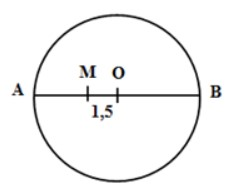
\includegraphics[scale=1.0]{../figs/giaothoasong-h1.jpg}
		\end{center}
		
		Sóng tại M có biên độ cực đại khi $d_2-d_1=k\lambda$.
		
		Ta có $d_1=\dfrac{15}{2}+\text{1,5}=9\,\text{cm}$; $d_2=\dfrac{15}{2}-\text{1,5}=6\,\text{cm}$.
		
		Khi đó $d_2-d_1=3\,\text{cm}$.
		
		Với điểm M gần O nhất, chọn $k=1$.
		
		Khi đó ta có: $\lambda=3\,\text{cm}$.
		
		Số điểm dao động với biên độ cực đại trên đoạn AB là	
		$$-\text{AB}< \text{d}_2-\text{d}_1<\text{AB}$$
		
		Hay $$-15 < k\lambda < 15 \Rightarrow -5 < k < 5$$
		
		Do đó có 9 giá trị $k$.
		
		Do đường kính của đường tròng tâm O là $\text{20}\,\text{cm}$ hai nguồn nằm trong đường tròn nên số điểm dao động với biên độ cực đại trên đường tròn là 18 điểm.
		
	}
	
	%%%%%%%%%%%Câu 2%%%%%%%%%%%%%%
	\item \mkstar{3}
	
	\cauhoi{	
		Hai nguồn sóng kết hợp giống hệt nhau được đặt cách nhau một khoảng cách $x$ trên đường kính của một vòng tròn bán kính $R$ ($x<R$) và đối xứng qua tâm của vòng tròn. Biết rằng mỗi nguồn đều phát sóng có bước sóng $\lambda$ và $x=6\lambda$. Số điểm dao động cực đại trên vòng tròn là
		
		\begin{mcq}(4)
			\item 26.
			\item 24.
			\item 22.
			\item 20.
		\end{mcq}
		
	}
	
	\loigiai{
		\textbf{Đáp án C.}
		
		\begin{center}
			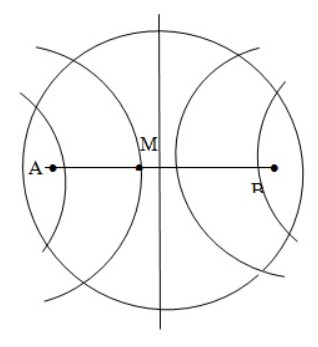
\includegraphics[scale=0.8]{../figs/giaothoasong-h2.jpg}
		\end{center}
		
		Xét điểm M trên AB ($\text{AB}=2x=12\lambda$): $\text{AM}=d_1$ và $\text{BM}=d_2$.
		
		Ta có: $d_1-d_2=k\lambda$ và $d_1+d_2=6\lambda$ nên $d_1=(3+0,5k)\lambda$.
		
		Mặt khác: $0\leq d_1\leq 6\lambda$ nên $-6\leq k \leq 6$.
		
		Số điểm dao động cực đại trên AB  là 13 điểm kể cả hai nguồn A, B, nhưng số đường cực đại cắt đường tròn chỉ có 11. Do đó, số điểm dao động cực đại trên vòng tròn là 22.
		
	}
	
	%%%%%%%%%%%Câu 3%%%%%%%%%%%%%%
	\item \mkstar{3}
	
	\cauhoi{
		
		Trên bề mặt chất lỏng có hai nguồn kết hợp AB cách nhau $40\,\text{cm}$ dao động cùng pha. Biết sóng do mỗi nguồn phát ra có tần số $f=10\,\text{Hz}$, vận tốc truyền sóng $2\,\text{m}/\text{s}$. Gọi M là một điểm  nằm trên đường vuông góc với AB tại đó A dao đông với biên độ cực đại. Đoạn AM có giá trị lớn nhất là
		
		
		\begin{mcq}(4)
			\item $20\,\text{cm}$.
			\item $30\,\text{cm}$.
			\item $40\,\text{cm}$.
			\item $50\,\text{cm}$.
		\end{mcq}
		
	}
	
	\loigiai{
		\textbf{Đáp án B.}
		
		\begin{center}
			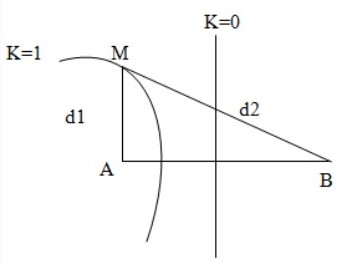
\includegraphics[scale=0.8]{../figs/giaothoasong-h3.jpg}
		\end{center}
		
		Ta có $\lambda = \dfrac{v}{f} = 20\,\text{cm}$.
		
		Do M là một cực đại giao thoa nên để  đoạn AM có giá trị lớn nhất thì M phải nằm trên vân cực đại bậc 1 như hình vẽ và thõa mãn
		$$d_2-d_1=k\lambda=20\,\text{cm}.$$
		
		Mặt khác, do tam giác AMB là tam giác vuông tại A nên ta có
		$$\text{BM}=d_2=\sqrt{\text{AB}^2+\text{AM}^2}=\sqrt{40^2+d_1^2}$$
		
		Từ đó ta suy ra được $d_1=30\,\text{cm}$.
	}
	
	%%%%%%%%%%%Câu 4%%%%%%%%%%%%%%
	\item \mkstar{3} 
	
	\cauhoi{	
		Trên mặt chất lỏng có hai nguồn sóng cùng tần số, cùng pha đặt tại hai điểm A và B. Cho bước sóng do các nguồn gây ra là $\lambda=5\,\text{cm}$. Trên nửa đường thẳng đi qua B trên mặt chất lỏng, hai điểm M và N (N gần B hơn), điểm M dao động với biên độ cực đại, N dao động với biên độ cực tiểu, giữa M và N có ba điểm dao động với biên độ cực đại khác. Biết hiệu $\text{MA}-\text{NA}=\text{1,2}\,\text{cm}$. Nếu đặt hai nguồn sóng này tại M và N thì số điểm dao động với biên độ cực đại trên đoạn thẳng AB là	
		\begin{mcq}(4)
			\item 3.
			\item 4.
			\item 1.
			\item 2.
		\end{mcq}
		
	}
	
	\loigiai{
		\textbf{Đáp án A.}
		\begin{center}
			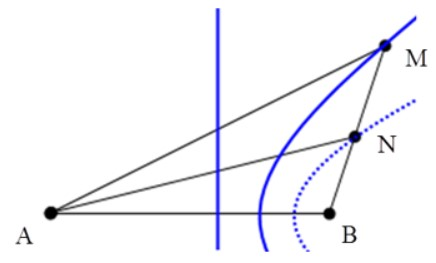
\includegraphics[scale=0.8]{../figs/giaothoasong-h4.jpg}
		\end{center}
		
		M thuộc cực đại và N thuộc cực tiểu nên ta có
		$$\begin{cases}
			\text{AM}-\text{BM}=k\lambda\\
			\text{AN}-\text{BN}=\left[(k+3)+\dfrac{1}{2}\right]\lambda
		\end{cases}
		\Rightarrow\text{MN}=\text{18,7}\,\text{cm}.$$
		
		Với nguồn đặt tại M, N. Xét đoạn AB, ta có
		$$\text{MA}-\text{NA}\leq k\lambda \leq \text{MA}-\text{NB}$$
		$$\Rightarrow \text{0,24}\leq k\lambda \leq\text{3,74}.$$
		
		Vậy có 3 cực đại.
	}
	
	%%%%%%%%%%%Câu 5%%%%%%%%%%%%%%
	\item \mkstar{3}
	
	\cauhoi{
		Ở mặt thoáng của chất lỏng có hai nguồn sóng A, B cách nhau $18\,\text{cm}$, dao động theo phương thẳng đứng với phương trình $u_{\text A}=u_{\text B}=a\cos(20\pi t)$ ($t$ tính bằng s). Tốc độ truyền sóng trên mặt chất lỏng là $50\,\text{cm/s}$. Gọi M là điểm ở mặt chất lỏng gần A nhất sao cho phần tử chất lỏng tại M dao động với biên độ cực đại và cùng pha với nguồn A. Khoảng cách AM là
		\begin{mcq}(4)
			\item $\text{2,5}\,\text{cm}$.
			\item $2\,\text{cm}$.
			\item $5\,\text{cm}$.
			\item $\text{1,25}\,\text{cm}$.
		\end{mcq}
		
	}
	
	\loigiai{
		\textbf{Đáp án C.}
		
		Bước sóng là
		$$\lambda=\dfrac{v}{f}=5\,\text{cm}.$$
		Áp dụng kết quả bài toán điều kiện để một vị trí cực đại và cùng pha với nguồn
		$$\begin{cases}
			d_2-d_1=2k\lambda\\
			d_2+d_1=2m\lambda
		\end{cases}
		\textrm{  hoặc  }
		\begin{cases}
			d_2-d_1=(2k+1)\lambda\\
			d_2+d_1=(2m+1)\lambda
		\end{cases}
		\Rightarrow d_1=(m-k)\lambda.$$
		Do đó $d_{1\ \text{min}}$ khi
		$(m-k)_\text{min}\Rightarrow d_{1\ \text{min}}=\lambda=5\,\text{cm}.$
	}
	
	%%%%%%%%%%%Câu 6%%%%%%%%%%%%%%
	\item \mkstar{3}
	
	\cauhoi{	
		Tại hai điểm A, B trên mặt nước cách nhau $16\,\text{cm}$ có hai nguồn phát sóng giống nhau. Điểm M nằm trên mặt nước và trên đường trung trực của AB cách trung điểm I của AB một khoảng nhỏ nhất bằng $5\sqrt{5}\,\text{cm}$ luôn dao động cùng pha với I. Điểm N nằm trên mặt nước và nằm trên đường thẳng vuông góc với AB tại A, cách A một khoảng nhỏ nhất bằng bao nhiêu để N dao động với biên độ cực tiểu?
		\begin{mcq}(4)
			\item $\text{9,22}\,\text{cm}$.
			\item $\text{8,75}\,\text{cm}$.
			\item $\text{2,14}\,\text{cm}$.
			\item $\text{8,57}\,\text{cm}$.
		\end{mcq}
		
	}
	
	\loigiai{
		\textbf{Đáp án C.}
		
		\begin{center}
			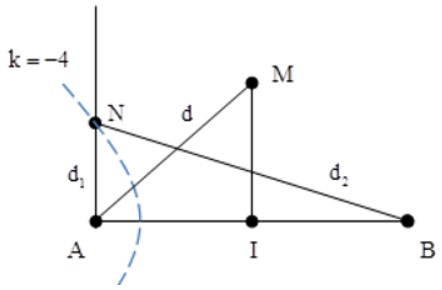
\includegraphics[scale=0.8]{../figs/giaothoasong-h5.jpg}
		\end{center}
		
		Vì hai nguồn đồng pha, M, I đều thuộc trung trực của AB nên để M và I dao động cùng pha thì
		$$\text{MA}-\text{IA}=k\lambda.$$
		M gần I nhất nên $k=1$, do đó
		$$\text{MA}=d_\text{A}=\text{0,5AB}+\lambda=8+\lambda.$$
		Mặt khác $\text{MI}=4\sqrt{5}\,\text{cm}$ nên
		$$\text{MA}=4\sqrt{5}\,\text{cm}\Rightarrow\text{MA}=8+\lambda=\sqrt{\left(\dfrac{\text{AB}}{2}\right)^2+\text{IM}^2}=12\Rightarrow\lambda=4\,\text{cm}.$$
		Số điểm dao động với biên độ cực tiểu trên AB
		$$-\dfrac{\text{AB}}{2}-\dfrac{1}{2}<k<\dfrac{\text{AB}}{2}-\dfrac{1}{2}\Rightarrow-\text{4,5}<k<\text{3,5}.$$
		Để N là một điểm cực tiểu và gần A nhất thì N phải nằm trên hypebol cực tiểu có $k=-4$
		$$\begin{cases}
			d_\text{1N}-d_\text{2N}=-3,5\lambda\\
			d^2_\text{2N}=d^2_\text{1N}+\text{AB}^2
		\end{cases}
		\Rightarrow d_\text{1N}=\text{2,14}\,\text{cm}.$$
	}
	
	%%%%%%%%%%%Câu 7%%%%%%%%%%%%%%
	\item \mkstar{3}
	
	\cauhoi{
		
		Ở mặt nước có hai nguồn kết hợp đặt tại hai điểm A và B, dao động cùng pha theo phương thẳng đứng, phát ra hai sóng có bước sóng $\lambda$. Trên AB có 9 vị trí mà ở đó các phần tử nước dao động với biên độ cực đại. C và D là hai điểm ở mặt nước sao cho ABCD là hình vuông. M là một điểm thuộc cạnh CD và nằm trên vân cực đại giao thoa bậc nhất $\left( \text{MA} -\text{MB}=\lambda\right) $. Biết phần tử tại M dao động cùng pha với các nguồn. Độ dài đoạn AB \textbf{gần nhất} với giá trị nào sau đây?
		
		\begin{mcq}(4)
			\item  $\text{4,6}\lambda$.
			\item $\text{4,8}\lambda$.
			\item $\text{4,4}\lambda$.
			\item $\text{4,7}\lambda$.
		\end{mcq}
		
	}
	
	\loigiai{
		\textbf{Đáp án B.}
		
		\begin{center}
			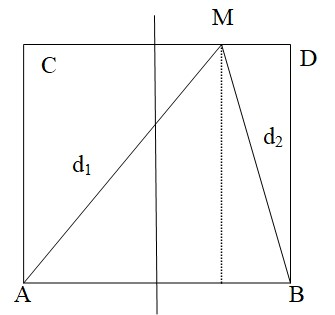
\includegraphics[scale=0.8]{../figs/giaothoasong-h6.jpg}
		\end{center}
		M là cực đại giao thoa và cùng pha với hai nguồn  nên $d_1-d_2=n\lambda, \ d_1+d_2=m\lambda$, với $n, \ m$ là số nguyên cùng lẻ hoặc cùng chẵn.
		
		Vì $n=1\Rightarrow m$ là số lẻ. 
		
		Ta có: $d_1+d_2>\text{AB}, \ 4\lambda \leq \text{AB} < 5\lambda$.
		
		Từ các phương trình trên, ta có: $d_1-d_2=\lambda, \ d_1+d_2=11\lambda$.
		
		Suy ra: $d_1=6\lambda, d_2=5\lambda$.
		
		Ta có:	$\sqrt{(6\lambda)^2-\text{AB}^2}+\sqrt{(5\lambda)^2-\text{AB}^2}=\text{AB}^2\Rightarrow \text{AB}=\text{4,8336}\lambda$.
	}
	%%%%%%%%%%%Câu 8%%%%%%%%%%%%%%
	\item \mkstar{3}
	
	\cauhoi{
		Ở mặt nước, tại hai điểm A và B có hai nguồn kết hợp dao động cùng pha theo phương thẳng đứng. ABCD là hình vuông nằm ngang. Biết trên CD có 3 vị trí mà ở đó các phần tử dao động với biên độ cực đại. Trên AB có tối đa bao nhiêu vị trí mà phần tử ở đó dao động với biên độ cực đại?
		\begin{mcq}(4)
			\item $13$.
			\item $7$.
			\item $11$.
			\item $9$.
		\end{mcq}
		
	}
	
	\loigiai{
		\textbf{Đáp án D.}
		
		Số cực đại trên CD là $a-a\sqrt{2}\leq k\leq a\sqrt{2}-a $.
		
		Chỉ có 3 cực đại $\Rightarrow k=2\Rightarrow \dfrac{a\left(\sqrt{2}-1 \right) }{\lambda}<2\Rightarrow \dfrac{a}{\lambda}<\text{4,8}$.
		
		Số cực đại trên AB là $-a\leq k\leq a\Leftrightarrow -\text{4,8}\leq k\leq \text{4,8}\leq \Rightarrow k=-4; -3,..;3,4$.
		
		Vậy số cực đại trên AB là $9$.
	}
	
	%%%%%%%%%%%Câu 9%%%%%%%%%%%%%%


	\item \mkstar{3}
	
	\cauhoi{
		
		Thực hiện thí nghiệm giao thoa sóng cơ trên mặt chất lỏng với 2 nguồn cùng pha có tần số $f=\SI{30}{Hz}$, vận tốc truyền sóng trong môi trường là 150 cm/s. Trên mặt chất lỏng có 4 điểm có tọa độ so với các nguồn lần lượt như sau: M ($d_1 =\SI{25}{cm}; d_2 = \SI{30}{cm}$); N ($d_1 =\SI{5}{cm}; d_2 = \SI{10}{cm}$); O ($d_1 =\SI{7}{cm}; d_2 = \SI{12}{cm}$); P ($d_1 =\SI{27,5}{cm}; d_2 = \SI{30}{cm}$). Hỏi có mấy điểm nằm trên đường cực đại số 1?	
		
		\begin{mcq}(4)
			\item 1.
			\item 2.
			\item 3.
			\item 4.
		\end{mcq}
		
	}
	
	\loigiai{
		\textbf{Đáp án C.}
		
		
		Ta có $\lambda = \dfrac{v}{f} = \SI{5}{cm}$. 
		
		Tại M: $\Delta d = d_2-d_1 =\SI{5}{cm} =\lambda \Rightarrow$ nằm trên đường cực đại số 1.
		
		Tại N: $\Delta d = d_2-d_1 =\SI{5}{cm} =\lambda \Rightarrow$ nằm trên đường cực đại số 1.
		
		Tại O: $\Delta d = d_2-d_1 =\SI{5}{cm} =\lambda \Rightarrow$ nằm trên đường cực đại số 1.
		
		Tại P: $\Delta d = d_2-d_1 =\SI{2,5}{cm} =\lambda \Rightarrow$ nằm trên đường cực tiểu số 1.
		
		Có 3 điểm M, N, O nằm trên cực đại số 1.
	}

	\item \mkstar{3}
	
	\cauhoi{
		Tại hai điểm A, B trên mặt chất lỏng cách nhau 15 cm có hai nguồn phát sóng kết hợp dao động theo phương trình $u_1 =a\cos 40\pi t\ \text{cm}$ và $u_2 = b\cos (40\pi t +\pi)\ \text{cm}$. Tốc độ truyền sóng trên bề mặt chất lỏng 40 cm/s. Gọi E, F là 2 điểm trên đoạn AB sao cho AE = EF = FB. Tìm số cực đại trên EF.
		\begin{mcq}(4)
			\item 5.
			\item 6.
			\item 4.
			\item 7.
		\end{mcq}
		
	}
	
	\loigiai{
		\textbf{Đáp án B.}
		
		Tại E ($d_1 =\SI{5}{cm}; d_2=\SI{10}{cm}$) suy ra $\Delta d_\text{E} = \SI{5}{cm}$.
		
		Tại F ($d_1 =\SI{10}{cm}; d_2=\SI{5}{cm}$) suy ra $\Delta d_\text{F} = \SI{-5}{cm}$.
		
		$\lambda = \dfrac{v}{f} =\SI{2}{cm}$.
		
		Vì 2 nguồn dao động ngược pha: $\Delta \varphi =\pi\ \text{rad}$.
		
		Số cực đại: $\dfrac{\Delta d_\text{F}}{\lambda}-\dfrac{\Delta \varphi}{2\pi} \leq k \leq \dfrac{\Delta d_\text{E}}{\lambda}-\dfrac{\Delta \varphi}{2\pi} \Rightarrow -3 \leq k \leq 2$.
		
		Có 6 điểm dao động cực đại.
	}

	\item \mkstar{3}
	
	\cauhoi{
		
		Thực hiện thí nghiệm giao thoa sóng cơ trên mặt nước với hai nguồn cùng pha có tần số là 10 Hz. M là điểm cực tiểu có khoảng cách đến nguồn 1 là $d_1=\SI{25}{cm}$ và cách nguồn 2 là $d_2 = \SI{40}{cm}$. Biết giữa M và đường trung trực còn có 1 cực đại nữa. Xác định vận tốc truyền sóng trên mặt nước.
		
		\begin{mcq}(4)
			\item 50 m/s.
			\item 0,5 m/s.
			\item 5 cm/s.
			\item 50 mm/s.
		\end{mcq}
		
	}
	
	\loigiai{
		\textbf{Đáp án B.}
		
		Vì M nằm trên đường cực tiểu giữa M và đường trung trực còn có 1 cực đại nữa, nên M nằm trên đường cực tiểu số 2.
		
		Ta có: $\Delta d = d_2-d_1 =\left(1+\dfrac{1}{2}\right)\lambda.$
		
		Bước sóng $\lambda =\SI{5}{cm}$.
		
		Vận tốc truyền sóng: $v=\lambda f =50\ \text{cm/s}$.
	}
	\item \mkstar{3}
	
	\cauhoi{
		Thực hiện thí nghiệm giao thoa sóng trên mặt nước với hai nguồn sóng cùng pha S$_1$S$_2$ cách nhau $6\lambda$. Hỏi trên S$_1$S$_2$ có bao nhiêu điểm dao động cực đại và cùng pha với nguồn?
		
		
		\begin{mcq}(4)
			\item 13.
			\item 6.
			\item 7.
			\item 12.
		\end{mcq}
		
	}
	
	\loigiai{
		\textbf{Đáp án C.}
		
		Gọi M là điểm nằm trên đường cực đại.
		
		$d_1$ là khoảng cách từ nguồn S$_1$ tới M; $d_2$ là khoảng cách từ nguồn 2 tới điểm M.
		
		$u_1=u_2= U_0 \cos \omega t.$
		
		$d_1+d_2 = 6\lambda$. (1)
		
		Suy ra $u_\text{M} = 2U_0 \cos \dfrac{\pi(d_2-d_1)}{\lambda} \cos (\omega t -6\pi)$.
		
		Để M cùng pha với nguồn: $\cos \dfrac{\pi(d_2-d_1)}{\lambda} =1 \Rightarrow d_2 -d_1 =2k\lambda\ (2).$
		
		Từ (1) và (2) suy ra $d_2 = (k+3)\lambda$.
		
		Vì $0\leq d_2 \leq 6\lambda \Rightarrow -3\leq k \leq 3$.
		
		Có 7 điểm cực đại.
	}
	\item \mkstar{3}
	
	\cauhoi{
		
		Thực hiện thí nghiệm giao thoa sóng trên mặt nước với hai nguồn sóng cùng pha S$_1$S$_2$ cách nhau $6\lambda$. Hỏi trên S$_1$S$_2$ có bao nhiêu điểm dao động cực đại và ngược pha với nguồn?
		\begin{mcq}(4)
			\item 13.
			\item 6.
			\item 7.
			\item 12.
		\end{mcq}
		
	}
	
	\loigiai{
		\textbf{Đáp án B.}
		
		$u_1=u_2= U_0 \cos \omega t.$
		
		$d_1+d_2 = 6\lambda$. (1)
		
		Để M cực đại: $\cos \dfrac{\pi(d_2-d_1)}{\lambda} = \pm 1.$
		
		Để M ngược pha so với nguồn: $\cos \dfrac{\pi(d_2-d_1)}{\lambda} = - 1 \Rightarrow d_2-d_1 =(2k+1) \lambda\ (2)$.
		
		Từ (1) và (2) suy ra $d_2 =\left (k+3+\dfrac{1}{2}\right) \lambda.$
		
		Vì $0 \leq \left (k+3+\dfrac{1}{2}\right) \lambda \leq 6\lambda $. 
		
		Có 6 điểm.
		
	}
	\item \mkstar{3}
	
	\cauhoi{
		
		Hai mũi nhọn S$_1$S$_2$ cách nhau 9 cm, gắn ở đầu một cần rung có tần số $f=\SI{100}{Hz}$ được đặt cho chạm nhẹ vào mặt một chất lỏng. Vận tốc truyên sóng trên mặt chất lỏng là 0,8 m/s. Gõ nhẹ cho cần rung thì 2 điểm S$_1$, S$_2$ dao động theo phương thẳng đứng với phương trình dạng $u=a\cos 2\pi ft$. Điểm M trên mặt chất lỏng cách đều và dao động cùng pha S$_1$, S$_2$ gần S$_1$, S$_2$ nhất. Xác định khoảng cách của M đến S$_1$S$_2$.
		
		\begin{mcq}(4)
			\item 2,79 cm.
			\item 6,17 cm.
			\item 7,16 cm.
			\item 1,67 cm.
		\end{mcq}
		
	}
	
	\loigiai{
		\textbf{Đáp án D.}
		
		$\lambda =\dfrac{v}{f} =\SI{0,8}{cm}$.
		
		Vì $d_1=d_2=d$.
		
		Để M cùng pha với nguồn $\dfrac{2\pi d}{\lambda} = k2\pi$.
		
		$k = \dfrac{d}{\lambda} \geq \text{5,625}$.
		
		M gần S$_1$S$_2$ nhất nên $k=6$.
		
		$d=d_1=d_2 =k\lambda =\SI{4,8}{cm}$.
		
		Khoảng cách gần nhất là
		
		$\sqrt{\text{4,8}^2-\text{4,5}^2} =\SI{1,67}{cm}$.
	}
	\item \mkstar{3}
	
	\cauhoi{
		
		Thực hiện thí nghiệm giao thoa sóng cơ với hai nguồn S$_1$S$_2$ cùng pha cách nhau 4 m. Tần số của hai nguồn là 10 Hz, vận tốc truyền sóng trong môi trường là 16 m/s. M nằm trên đường thẳng kẻ từ S$_1$ đường thẳng vuông góc với S$_1$S$_2$, và M là điểm cực đại. Hãy tìm khoảng cách MS$_1$ nhỏ nhất.
		
		\begin{mcq}(4)
			\item 4,1 cm.
			\item 4 cm.
			\item 0,9 cm.
			\item 5,1 cm.
		\end{mcq}
		
	}
	
	\loigiai{
		\textbf{Đáp án C.}
		
		$\lambda =\dfrac{v}{f} =\SI{1,6}{m}$.
		
		Số đường cực đại: $-\dfrac{d}{\lambda} \leq k \leq \dfrac{d}{\lambda} \Rightarrow \text{2,5} \leq k \leq \text{2,5}$. 
		
		Vậy những đường cực đại là -2; -1; 0; 1; 2.
		
		Vì M nằm trên đường cực đại và gần S$_1$S$_2$ nhất nên M phải nằm trên đường số 2.
		
		$d_2 -d_1 =2\lambda = \text{3,2}$; $d_2^2-d^2_1 =42$.
		
		Suy ra $d_2 =\SI{4,1}{cm}; d_1 =\SI{0,9}{cm}$.
	}

	\item \mkstar{3}
	
	\cauhoi{
		Trong hiện tượng giao thoa sóng nước, 2 nguồn kết hợp A, B cách nhau 20 cm dao động điều hòa cùng pha, cùng tần số 40 Hz. Tốc độ truyền sóng là 1,2 m/s. Xét trên đường tròn tâm A, bán kính AB, điểm nằm trên đường tròn dao động với biên độ cực đại, cách đường trung trực AB một khoảng ngắn nhất bằng bao nhiêu?
		\begin{mcq}(4)
			\item 27,75 mm.
			\item 26,1 mm.
			\item 19,76 mm.
			\item 32,4 mm.
		\end{mcq}
		
	}
	
	\loigiai{
		\textbf{Đáp án A.}
		
		Ta có: $\lambda =\dfrac{v}{f} = \SI{3}{cm}$.
		
		Vì M cực đại nên $d_2-d_1 =n\lambda$.
		
		Vì M gần đường trung trực nhất nên $n=-1 \Rightarrow  d_2 - d_1 = \SI{-3}{cm}$.
		
		Áp dụng hệ thức lượng, tìm được khoảng cách từ M đến đường trung trực AB là $\SI{27.75}{mm}$.
	}

	\item \mkstar{4}

\cauhoi{
	
	Giao thoa sóng ở mặt nước với hai nguồn kết hợp đặt tại A và B. Hai
	nguồn dao động điều hòa theo phương thẳng đứng, cùng pha và cùng tần số $\SI{10}{Hz}$. Biết $\text{AB}=\SI{20}{cm}$, tốc độ truyền sóng ở mặt nước là $\SI{0,3}{m/s}$. Ở mặt nước, gọi $\Delta$ là đường thẳng đi qua
	trung điểm của AB và hợp với AB một góc $60^\circ$. Trên $\Delta$ có bao nhiêu điểm mà các phần tử ở đó dao động với biên độ cực đại?
	\begin{mcq}(4)
		\item 7 điểm.
		\item 11 điểm.
		\item 13 điểm.
		\item 9 điểm.
	\end{mcq}
	
}

\loigiai{
	\textbf{Đáp án A.}
	
	\begin{center}
		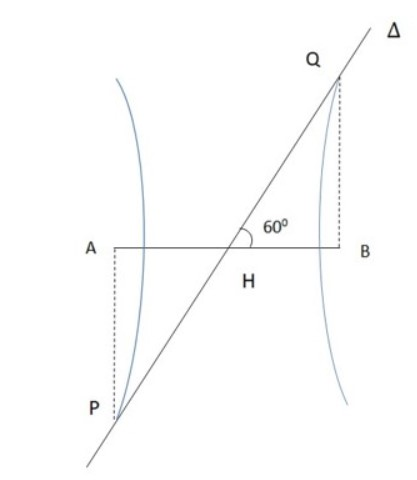
\includegraphics[scale=0.8]{../figs/giaothoasong-h7.jpg}
	\end{center}
	
	Ta có:
	
	$$\text{PA}=\text{QB}=\text{HB}\tan {{60}^\circ}=10\sqrt{3}\,\text{cm}.$$
	
	$$\text{PB}=\text{QA}=\sqrt{A{{B}^{2}}+P{{A}^{2}}}=10\sqrt{7}\,\text{cm}.$$
	
	Bước sóng là
	$$\lambda =\dfrac{v}{f}=3\,\text{cm}.$$
	
	Vì hai nguồn cùng pha nên:
	
	$$\Delta {{d}_\text{P}}\le k\lambda \le \Delta {{d}_\text{Q}}$$		
	$$\Rightarrow \text{PA}-\text{PB}\le k\lambda \le \text{QA}-\text{QB}$$		
	$$\Rightarrow 10\sqrt{3}-10\sqrt{7}\le 3k\le 10\sqrt{7}-10\sqrt{3}$$		
	$$\Rightarrow \dfrac{10\sqrt{3}-10\sqrt{7}}{3}\le k\le \dfrac{10\sqrt{7}-10\sqrt{3}}{3}$$		
	$$\Rightarrow -3,05\le k\le 3,05$$		
	$$\Rightarrow k\in \left\{ 0;\pm 1;\pm 2;\pm 3 \right\}$$
	
	Vậy có 7 điểm dao động với biên độ cực đại.
}
%%%%%%%%%%%Câu 10%%%%%%%%%%%%%%
\item \mkstar{4}

\cauhoi{
	
	Tại mặt chất lỏng, hai nguồn $\text{S}_1$, $\text{S}_2$ cách nhau $13\,\text{cm}$ dao động theo phương thẳng đứng với phương trình $u_1=u_2=A\cos 40\pi t\ \text{cm}$ ($t$ tính bằng s). Tốc độ truyền sóng trên mặt chất lỏng là $80\,\textrm{cm/s}$. Ở mặt chất lỏng, gọi $\Delta$ là đường trung trực của S$_1$S$_2$. M là một điểm không nằm trên $\text{S}_1\text{S}_2$ và không thuộc $\Delta$, sao cho phần tử chất lỏng tại M dao động với biên độ cực đại và cùng pha với hai nguồn. Khoảng cách ngắn nhất từ M đến $\Delta$ là
	\begin{mcq}(4)
		\item $\text{2,00}\,\text{cm}$.
		\item $\text{2,46}\,\text{cm}$.
		\item $\text{3,07}\,\text{cm}$.
		\item $\text{4,92}\,\text{cm}$.
	\end{mcq}
	
}

\loigiai{
	\textbf{Đáp án C.}
	
	\begin{center}
		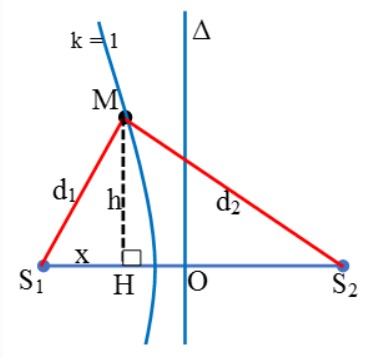
\includegraphics[scale=0.8]{../figs/giaothoasong-h8.jpg}
	\end{center}
	
	Điều kiện để M dao động cực đại và đồng pha với hai nguồn là
	$$\begin{cases}
		d_2-d_1=k\lambda\\
		d_1+d_2=n\lambda.
	\end{cases}$$
	với $n$, $k$ cùng chẵn hoặc cùng lẻ.
	
	Để M gần $\Delta$ nhất thì $k = 1$ và $n$ khi đó có thể nhận các giá trị lẻ 1, 3…..thỏa mãn bất đẳng thức tam giác
	$$d_1+d_2>\text{S}_1\text{S}_2=13\Rightarrow n>\dfrac{13}{\lambda}\Rightarrow n>\text{3,25}.$$
	
	Vậy $n_\text{min}=5$ (do $n$ lẻ).
	
	Ta có:
	$$\begin{cases}
		d_2-d_1=4\\
		d_1+d_2=20
	\end{cases}
	\Rightarrow
	\begin{cases}
		d_2=12\,\text{cm}\\
		d_1=8\,\text{cm}.
	\end{cases}$$
	
	Từ hình vẽ:
	$$\begin{cases}
		d_1^2=8^2=x^2+h^2\\
		d_2^2=12^2=(13-x)^2+h^2
	\end{cases}
	\Rightarrow x=\text{3,42}\,\text{cm}.$$
	
	Vậy khoảng cách giữa M và $\Delta$ khi đó bằng
	$$\text{HO}=\text{OS}_1-\text{S}_1\text{H}=\dfrac{13}{2}-\text{3,42}=\text{3,07}\,\text{cm}.$$
}
	
\end{enumerate}
\loigiai{\textbf{Đáp án}
	\begin{center}
		\begin{tabular}{|m{2.8em}|m{2.8em}|m{2.8em}|m{2.8em}|m{2.8em}|m{2.8em}|m{2.8em}|m{2.8em}|m{2.8em}|m{2.8em}|}
			\hline
			1. C & 2. B & 3. C & 4. D & 5. C & 6. C  & 7. B  & 8. B & 9. D & 10. A\\
			\hline
			11. B & 12. B & 13. A & 14. C & 15. B & 16. A  & 17. C  & 18. C & 19. B & 20. D\\
			\hline
			21. C & 22. B & 23. B & 24. C & 25. B & 26. D  & 27. C  & 28. A & 29. A & 30. C\\
			\hline
		\end{tabular}
\end{center}}
\stopcontents[mychapters]
\setcounter{mychapter}{8}
\mychapter{Sóng dừng}
\startcontents[mychapters]
\printcontents[mychapters]{}{0}{\setcounter{tocdepth}{1}}
\begin{enumerate}[label=\bfseries Câu \arabic*:]
\item \mkstar{1}

\cauhoi{ 
	
	Trên một dây có hiện tượng sóng dừng thì 
	
	
	\begin{mcq}
		\item tất cả các điểm trên dây đều chuyển động với cùng một tốc độ.
		\item tất cả các điểm trên dây đều dao động với biên độ cực đại.
		\item tất cả phần tử trên dây đều đứng yên.
		\item xuất hiện trên dây có những bụng sóng xen kẽ với nút sóng.
	\end{mcq}
	
}
\loigiai{\textbf{Đáp án: D.}

Trên một dây có hiện tượng sóng dừng thì xuất hiện trên dây có những bụng sóng xen kẽ với nút sóng.
}	
	\item \mkstar{2}

\cauhoi{
	
	Chọn câu trả lời \textbf{đúng}. Người ta nói sóng dừng là một trường hợp đặc biệt của giao thoa sóng vì
	
	\begin{mcq}
		\item sóng dừng là sự giao thoa của các sóng trên cùng một phương truyền sóng.  
		\item sóng dừng là sự chồng chất của các sóng trên cùng một phương truyền sóng.
		\item sóng dừng xảy ra khi có sự giao thoa của sóng tới và sóng phản xạ trên cùng một phương truyền sóng. 
		\item sóng dừng là sự giao thoa của các sóng trên cùng một phương truyền sóng. 
	\end{mcq}
	
}

\loigiai{
	\textbf{Đáp án: C.}
	
	Người ta nói sóng dừng là một trường hợp đặc biệt của giao thoa sóng vì sóng dừng xảy ra khi có sự giao thoa của sóng tới và sóng phản xạ trên cùng một phương truyền sóng. 
}
\item \mkstar{2}

\cauhoi{
	Chọn câu trả lời \textbf{đúng}. Ứng dụng của hiện tượng sóng dừng để 
	
	\begin{mcq} (2)
		\item xác định tốc độ truyền sóng.   
		\item xác định chu kì sóng.
		\item xác định tần số sóng.
		\item xác định năng lượng sóng. 
	\end{mcq}
	
}

\loigiai{
	\textbf{Đáp án A.}
	
	Ứng dụng của hiện tượng sóng dừng để xác định tốc độ truyền sóng. 
}
\item \mkstar{2}

\cauhoi{
	
	Một sợi dây đàn hồi AB có chiều dài 120 cm, có đầu B cố định, đầu A được gắn với một bản rung tần số $f$. Trên dây có sóng dừng với 4 bụng sóng. Biên độ tại bụng là 5 cm. Tại điểm C trên dây gần B nhất có biên độ dao động là 2,5 cm. Hỏi CB có giá trị bao nhiêu?
	\begin{mcq}(4)
		\item 7,5 cm.
		\item 5 cm.
		\item 35 cm.
		\item 25 cm.
	\end{mcq}
	
}

\loigiai{
	\textbf{Đáp án B.}
	
	Ta có $4\dfrac{\lambda}{2}=120 \Rightarrow \lambda =\SI{60}{cm}$.
	
	Số bụng gần nút B nhất cách B một khoảng $\dfrac{\lambda}{4} =\SI{15}{cm}$.
	
	$\text{CB} =\SI{5}{cm}$.
}
\item \mkstar{2}

\cauhoi{
	
	Một sợi dây mảnh đàn hồi AB dài 2,5 m được căng theo phương ngang, trong đó đầu B cố định, đầu A được rung nhờ một dụng cụ để tạo sóng dừng trên dây. Tần số rung $f$ có thể thay đổi được giá trị trong khoảng 93 Hz đến 100 Hz. Biết tốc độ truyền sóng trên dây là 24 m/s. Hỏi tần số $f$ phải nhận giá trị nào dưới đây để trên dây có sóng dừng?
	\begin{mcq}(4)
		\item 94 Hz.
		\item 96 Hz.
		\item 98 Hz.
		\item 100 Hz.
	\end{mcq}
	
}

\loigiai{
	\textbf{Đáp án B.}
	
	Ta có sóng dừng 2 đầu cố định $l=k\dfrac{\lambda}{2} = \dfrac{kv}{2f} \Rightarrow f = \dfrac{kv}{2l} = \text{9,6} k.$
	
	Theo đề bài $93 <f<100 \Rightarrow \text{9,68} <k<\text{10,41}$.
	
	$k$ là số nguyên nên $k=10$, $f=\SI{96}{Hz}$.
}
\item \mkstar{2}

\cauhoi{
	
	Một sóng cơ truyền trên một sợi dây rất dài thì một điểm M trên sợi dây có vận tốc dao động biến thiên theo phương trình $v_\text{M}= 20\pi \cos (10\pi t + \varphi)\ \text{cm/s}$. Giữ chặt một điểm trên dây sao cho trên dây hình thành sóng dừng, khi đó bề rộng một bụng sóng có độ lớn là
	\begin{mcq}(4)
		\item 8 cm.
		\item 6 cm.
		\item 10 cm.
		\item 4 cm.
	\end{mcq}
	
}

\loigiai{
	\textbf{Đáp án A.}
	
	Ta có phương trình vận tốc $v_\text{M}= 20\pi \cos (10\pi t + \varphi)\ \text{cm/s}$.
	
	Suy ra $A=\SI{2}{cm}$.
	
	Bề rộng bụng sóng là $4A =\SI{8}{cm}$.
}
\item \mkstar{2}

\cauhoi{
	
	Một sợi dây đàn hồi dài $\SI{90}{cm}$ có một đầu cố định và một đầu tự do đang có sóng dừng. Kể cả đầu cố định, trên dây có 8 nút. Biết rằng khoảng thời gian giữa 6 lần liên tiếp sợi dây duỗi thẳng là $\SI{0.25}{\second}$. Tốc độ truyền sóng trên dây là
	\begin{mcq} (4)
		\item $\SI{1.2}{\meter/\second}$.
		\item $\SI{2.9}{\meter/\second}$.
		\item $\SI{2.4}{\meter/\second}$.
		\item $\SI{2.6}{\meter/\second}$.
	\end{mcq}
	
}

\loigiai{
	\textbf{Đáp án: C.}
	
	Khoảng thời gian giữa 6 lần liên tiếp sợi dây duỗi thẳng là $\SI{0.25}{\second}$ nên
	\begin{equation*}
		5\cdot\dfrac{T}{2}=\SI{0.25}{\second}\Rightarrow T=\SI{0.1}{\second}.
	\end{equation*}
	
	Điều kiện để có sóng dừng trên một sơi dây có một đầu cố định, một đầu tự do là chiều dài của sợi dây phải bằng một số lẻ lần $\dfrac{\lambda}{4}$
	\begin{equation*}
		l=(2k+1)\dfrac{\lambda}{4},\qquad(k=0,1,2,3,\ldots),
	\end{equation*}
	trong đó: $k$ là số bó sóng nguyên.
	
	Dây dài $\SI{90}{cm}$, gồm một đầu cố định và một đầu tự do. Kể cả đầu cố định, trên dây có 8 nút nên trên dây có 7 bó sóng nguyên
	\begin{equation*}
		l=(2\cdot 7 +1)\cdot\dfrac{\lambda}{4}=\SI{0.9}{\meter}\Rightarrow\lambda=\SI{0.24}{\meter}.
	\end{equation*}
	
	Tốc độ truyền sóng trên dây là
	\begin{equation*}
		v=\dfrac{\lambda}{T}=\dfrac{\SI{0.24}{\meter}}{\SI{0.1}{\second}}=\SI{2.4}{\meter/\second}.
	\end{equation*}
	
	
}
\item \mkstar{2}

\cauhoi{
	
	Trên một sợi dây đàn hồi dài có sóng dừng với bước sóng $\SI{1.4}{cm}$. Trên dây có hai điểm A và B cách nhau $\SI{5.6}{cm}$. Biết A, B là một bụng. Số nút sóng và bụng sóng trên đoạn dây AB là
	\begin{mcq} (2)
		\item 8 nút và 9 bụng.
		\item 9 nút và 8 bụng.
		\item 9 nút và 10 bụng.
		\item 10 nút và 9 bụng.
	\end{mcq}	
}

\loigiai{
	\textbf{Đáp án A.}
	
	Ta có: $\text{AB}=4\lambda=8\cdot\dfrac{\lambda}{2}.$
	
	Vì $k=8$ nên trên dây có 8 bó sóng nguyên và A,B là bụng sóng nên trên dây AB có 8 nút sóng và 9 bụng sóng.
}
\item \mkstar{2}

\cauhoi{
	
	Trên một sợi dây đàn hồi dài có sóng dừng với bước sóng $\SI{1.2}{cm}$. Trên dây có hai điểm A và B cách nhau $\SI{6.1}{cm}$, tại A là một nút sóng. Số nút sóng và bụng sóng trên đoạn dây AB là
	\begin{mcq}(2)
		\item 10 nút và 9 bụng.
		\item 9 nút và 10 bụng.
		\item 10 nút và 11 bụng.
		\item 11 nút và 10 bụng.
	\end{mcq}
	
}

\loigiai{
	\textbf{Đáp án D.}
	
	Ta có: $\text{AB}=10\cdot\dfrac{\lambda}{2}+0,1.$
	
	Vì $k=10$ nên trên AB có 10 bó sóng nguyên mà $\SI{0,1}{cm}<\dfrac{\lambda}{4}$ nên trên đoạn dây AB ta có 11 nút sóng và 10 bụng sóng.
	
}

\item \mkstar{2}

\cauhoi{
	
	Thực hiện thí nghiệm sóng dừng trên sợi dây có hai đầu cố định có chiều dài 90 cm. Tần số của nguồn sóng là 10 Hz thì thấy trên dây có 2 bụng sóng. Xác định vận tốc truyền sóng trên dây
	
	\begin{mcq}(4)
		\item 9 m/s.
		\item 8 m/s.
		\item 4,5 m/s.
		\item 90 cm/s.
	\end{mcq}
	
}

\loigiai{
	\textbf{Đáp án A.}
	
	$l =k\dfrac{\lambda}{2} \Rightarrow \lambda =\SI{90}{cm}$.
	
	$v=\lambda f =9\ \text{m/s}$.
}
\item \mkstar{2}

\cauhoi{
	
	Một sợi dây đàn hồi, hai tần số liên tiếp có sóng dừng trên dây là 50 Hz và 70 Hz. Hãy xác định tần số nhỏ nhất có sóng dừng trên dây.
	\begin{mcq}(4)
		\item 10 Hz.
		\item 20 Hz.
		\item 30 Hz.
		\item 40 Hz.
	\end{mcq}
	
}

\loigiai{
	\textbf{Đáp án B.}
	
	Tần số $f=\dfrac{kv}{2l} \Rightarrow f_{k+1} -f_k = f_\text{min} = \SI{20}{Hz}$.
	
}
\item \mkstar{2}

\cauhoi{
	
	Một dây AB dài 90 cm có đầu B thả tự do. Tạo ở đầu A một dao động điều hòa ngang có tần số 100 Hz ta có sóng dừng, trên dây có 4 múi nguyên. Vận tốc truyền sóng trên dây có giá trị bao nhiêu?
	\begin{mcq}(4)
		\item 20 m/s.
		\item 40 m/s.
		\item 30 m/s.
		\item 60 m/s.
	\end{mcq}
	
}

\loigiai{
	\textbf{Đáp án B.}
	
	Ta có: $l = \left(k+\dfrac{1}{2}\right) \dfrac{\lambda}{2}$.
	
	$k=4$ suy ra $\lambda =\SI{40}{cm}$.
	
	Suy ra vận tốc $v=\lambda f = 40\ \text{m/s}$.
	
}
\item \mkstar{3}

\cauhoi{
	
	Một sợi dây CD dài 1 m, đầu C cố định, đầu D gắn với cần rung với tần số thay đổi được. D được coi là nút sóng. Ban đầu trên dây có sóng dừng. Khi tần số tăng thêm 20 Hz thì số nút trên dây tăng thêm 7 nút. Sau khoảng thời gian bằng bao nhiêu sóng phản xạ từ C truyền hết một lần chiều dài sợi dây?
	\begin{mcq}(4)
		\item 0,175 s.
		\item 0,07 s.
		\item 0,5 s.
		\item 1,2 s.
	\end{mcq}
	
}

\loigiai{
	\textbf{Đáp án A.}
	
	Ta có $l=k\dfrac{\lambda}{2} = \dfrac{kv}{2f} = \dfrac{(k+7)v}{f+20} \Rightarrow \dfrac{7}{k} =\dfrac{20}{f} \Rightarrow k = \dfrac{7f}{20} \Rightarrow l=\dfrac{7v}{40}$.
	
	Thời gian sóng truyền hết sợi dây
	
	$t =\dfrac{l}{v}=\SI{0,175}{s}$.
}

\item \mkstar{3}

\cauhoi{
	
	Một sợi dây đàn hồi căng thẳng đứng đầu dưới cố định đầu trên gắn với một nhánh của âm thoa dao động với tần số 12 Hz, thấy trên dây xảy ra sóng dừng với 7 nút sóng. Thả cho đầu dưới của dây tự do để trên dây vẫn xảy ra sóng dừng với 7 nút sóng thì tần số của âm thoa phải
	\begin{mcq}(2)
		\item tăng lên 1 Hz.
		\item giảm xuống 1 Hz.
		\item giảm xuống 1,5 Hz.
		\item tăng lên 1,5 Hz.
	\end{mcq}
	
}

\loigiai{
	\textbf{Đáp án A.}
	
	Khi 2 đầu cố định $l = 6 \dfrac{v}{2\cdot 12} (1)$.
	
	Khi 1 đầu cố định $l=\text{6,5} \dfrac{v}{2f}(2)$.
	
	Chia (1) cho (2) ta được $f=\SI{13}{Hz}$.
	
	Vậy phải tăng thêm 1 Hz.
}
\item \mkstar{3}

\cauhoi{
	
	Trên dây AB xảy ra sóng dừng. Đầu A gắn vào 1 âm thoa, đầu B để tự do. Chiều dài dây $L$. Quan sát trên dây thấy có 5 bụng sóng. Tổng độ dài của các phần tử dây dao động ngược pha với điểm B là 
	\begin{mcq}(4)
		\item $\dfrac{5L}{9}$.
		\item $\dfrac{5L}{4}$.
		\item $\dfrac{4L}{9}$.
		\item $\dfrac{4L}{5}$.
	\end{mcq}
	
}

\loigiai{
	\textbf{Đáp án C.}
	
	Đối với 1 đầu cố định 1 đầu tự do $\text{4,5} \dfrac{\lambda}{2} = L \Rightarrow \dfrac{\lambda}{2} =\dfrac{L}{\text{4,5}}$.
	
	Các phần tử dây dao động ngược pha với B có tổng độ dài bằng
	
	$2\cdot \dfrac{\lambda}{2} = \dfrac{2L}{\text{4,5}} =\dfrac{4L}{9}$.
}


\item \mkstar{3}

\cauhoi{
	
	Một sợi dây đàn hồi dài 1 m được treo lơ lửng lên một cần rung, cần có thể rung theo phương ngang với tần số thay đổi được từ 100 Hz đến 120 Hz. Vận tốc truyền sóng trên dây là 8 m/s. Trong quá trình thay đổi tần số rung của cần, có thể tạo ra được bao nhiêu lần sóng dừng trên dây với số bụng khác nhau?
	\begin{mcq}(4)
		\item 7.
		\item 4.
		\item 5.
		\item 6.
	\end{mcq}
	
}

\loigiai{
	\textbf{Đáp án C.}
	
	Dây treo lơ lững tức 1 đầu cố định, 1 đầu tự do.
	
	$l=(2k+1) \dfrac{\lambda}{4} = (2k+1) \dfrac{v}{4f}$.
	
	$\Rightarrow 100 \leq \dfrac{(2k+1)v}{4l} \leq 120.$
	
	$\Rightarrow \text{24,5} \leq k \leq \text{29,5}$.
	
	Có 5 giá trị của $k$ thỏa mãn hay có thể tạo ra được 5 lần sóng dừng.
}
\item \mkstar{3}

\cauhoi{
	
	Một sợi dây đàn hồi căng ngang, đang có sóng dừng ổn định. Khoảng thời gian giữa hai lần liên tiếp sợi dây duỗi thẳng là 0,1 s, tốc độ truyền sóng trên dây là 3 m/s. Khoảng cách giữa hai điểm gần nhau nhất trên sợi dây dao động cùng pha và có biên độ dao động bằng một nửa biên độ của bụng sóng là
	\begin{mcq}(4)
		\item 10 cm.
		\item 8 cm.
		\item 20 cm.
		\item 30 cm.
	\end{mcq}
	
}

\loigiai{
	\textbf{Đáp án C.}
	
	Khoảng thời gian giữa hai lần liên tiếp sợi dây duỗi thẳng là $\dfrac{T}{2} =\SI{0,1}{s} \Rightarrow T=\SI{0,2}{s} \Rightarrow \lambda =vT=\SI{0,6}{m}$.
	
	Khoảng cách từ một nút đến vị trí có biên độ bằng nửa biên độ cực đại $\dfrac{\lambda}{12}$.
	
	Hai điểm gần nhau nhất trên sợi dây dao động cùng pha suy ra 2 điểm thuộc cùng 1 bó sóng. 
	
	Khoảng cách cần tìm $\dfrac{\lambda}{2} - \dfrac{\lambda}{12}- \dfrac{\lambda}{12} =\dfrac{\lambda}{3} = \SI{20}{cm}$.
}
\item \mkstar{3}

\cauhoi{
	
	Trên một sợi dây có sóng dừng, điểm bụng M cách nút gần nhất N một đoạn 10 cm, khoảng thời gian giữa hai lần liên tiếp trung điểm P của đoạn MN có cùng li độ với điểm M là 0,1 s. Tốc độ truyền sóng trên dây là
	\begin{mcq}(4)
		\item 400 cm/s.
		\item 200 cm/s.
		\item 100 cm/s.
		\item 300 cm/s.
	\end{mcq}
	
}

\loigiai{
	\textbf{Đáp án B.}
	
	Bụng cách nút gần nhất $\dfrac{\lambda}{4} \Rightarrow \lambda = \SI{40}{cm}$.
	
	Khoảng thời gian giữa hai lần liên tiếp trung điểm P của đoạn MN có cùng li độ với M là:
	
	$\Delta t =\dfrac{T}{2} =\SI{0,1}{s} \Rightarrow T =\SI{0,2}{s}$.
	
	Tốc độ truyền sóng trên dây là 
	
	$v=\dfrac{\lambda}{T} = 2\ \text{m/s}$.
}
\item \mkstar{3}

\cauhoi{
	
	Trên một sợi dây dài 16 cm được tạo ra sóng dừng nhờ nguồn có biên độ 4 mm. Biên độ không đổi trong quá trình truyền sóng. Người ta đếm được trên sợi dây có 22 điểm dao động với biên độ 6 mm. Biết hai đầu sợi dây là hai nút. Số nút và bụng sóng trên dây là
	\begin{mcq}(2)
		\item 22 bụng và 23 nút.
		\item 8 bụng và 9 nút.
		\item 11 bụng và 12 nút.
		\item 23 bụng và 22 nút.
	\end{mcq}
	
}

\loigiai{
	\textbf{Đáp án C.}
	
	Trên mỗi bó có 2 điểm dao động với biên độ là 6 cm.
	
	Trên dây có 11 bó sóng.
	
	Trên dây có 11 bụng và 12 nút.
}
\item \mkstar{4}

\cauhoi{
	
	Một sợi dây đang có sóng dừng ổn định. Sóng truyền trên dây có tần số $\SI{10}{\hertz}$ và bước sóng $\SI{6}{\centi\meter}$. Trên dây, hai phần tử M và N có vị trí cân bằng cách nhau $\SI{8}{\centi\meter}$, M thuộc một bụng sóng dao
	động điều hoà với biên độ $\SI{6}{\milli\meter}$. Lấy $\pi^2=10$. Tại thời điểm $t$, phần tử M đang chuyển động với tốc độ $6\pi\,\text{cm/s}$ thì phần tử N chuyển động với gia tốc có độ lớn là
	\begin{mcq} (4)
		\item $6\sqrt{3}\,\text{m/}\text{s}^2$.
		\item $6\,\text{m/}\text{s}^2$.
		\item $6\sqrt{2}\,\text{m/}\text{s}^2$.
		\item $3\,\text{m/}\text{s}^2$.
	\end{mcq}
	
}

\loigiai{
	\textbf{Đáp án A.}
	
	Tần số góc của dao động là
	\begin{equation*}
		\omega=2\pi f=2\pi\cdot \SI{10}{\hertz} =20\pi\,\text{rad/s}.
	\end{equation*}
	
	Biên độ dao động của N là
	\begin{equation*}
		A_\text{M}= A_\text{b}\left|\cos\left( \dfrac{2\pi d}{\lambda}\right)\right|
		=\SI{0,006}{\meter}\cdot\left|\cos\left( \dfrac{2\pi\cdot \SI{0,08}{\meter}}{\SI{0,06}{\meter}}\right)\right|=\SI{0,003}{\meter}.
	\end{equation*}
	
	Tại thời điểm M chuyển động với tốc độ $6\pi\,\text{cm/s}$ thì đang có li độ là
	\begin{equation*}
		\left(\dfrac{x_\text{M}}{A_\text{M}}\right)^2+\left(\dfrac{v_\text{M}}{v_\textrm{M max}}\right)^2=1
		\Rightarrow \left(\dfrac{x}{\SI{0,006}{\meter}}\right)^2+\left(\dfrac{6\pi\cdot10^{-2}\,\text{m/s}}{20\pi\,\text{rad/s}\cdot \SI{0,006}{\meter}}\right)^2=1
		\Rightarrow x_\text{M}=\dfrac{3\sqrt{3}}{1000}\,\text{m}.
	\end{equation*}
	
	Gia tốc của điểm N có thể được suy ra bằng cách lập tỉ số giữa gia tốc của M và gia tốc của N
	\begin{equation*}
		\left|\dfrac{a_\text{N}}{a_\text{M}}\right| = \left|\dfrac{a_\text{N}}{\omega^2 x_\text{M}}\right| = \dfrac{A_\text{N}}{A_\text{M}}
		\Rightarrow \left|\dfrac{a_\text{N}}{(20\pi\,\text{rad/s})^2\cdot \dfrac{3\sqrt{3}}{1000}\,\text{m}}\right| = \dfrac{\SI{0,003}{\meter}}{\SI{0,006}{\meter}}
		\Rightarrow \left|a_\text{N}\right|=6\sqrt{3}\,\text{m/}\text{s}^2.
	\end{equation*}
}
\end{enumerate}
\loigiai{\textbf{Đáp án}
	\begin{center}
		\begin{tabular}{|m{2.8em}|m{2.8em}|m{2.8em}|m{2.8em}|m{2.8em}|m{2.8em}|m{2.8em}|m{2.8em}|m{2.8em}|m{2.8em}|}
			\hline
			1. D & 2. C & 3. A & 4. B & 5. B & 6. A  & 7. C  & 8. A & 9. D & 10. A\\
			\hline
			11. B & 12. B & 13. A & 14. A & 15. C & 16. C  & 17. C  & 18. B & 19. C & 20. A\\
			\hline
		\end{tabular}
\end{center}}
\stopcontents[mychapters]
\setcounter{mychapter}{9}
\mychapter{Đặc trưng vật lý của âm}
\startcontents[mychapters]
\printcontents[mychapters]{}{0}{\setcounter{tocdepth}{1}}
\begin{enumerate}[label=\bfseries Câu \arabic*:]

\item \mkstar{1}

\cauhoi{
	
	Khi con ruồi và con muỗi bay, ta nghe được tiếng vo ve từ muỗi bay mà không nghe được từ ruồi là do
	\begin{mcq}(1)
		\item tần số đập cánh của muỗi thuộc vùng tai người nghe được.
		\item muỗi bay tốc độ chậm hơn ruồi.
		\item muỗi phát ra âm thanh từ cánh.
		\item muỗi đập cánh đều đặn hơn ruồi.
	\end{mcq}
}
\loigiai{
	
	\textbf{Đáp án A.}
	
	
	
	Khi con ruồi và con muỗi bay, ta nghe được tiếng vo ve từ muỗi bay mà không nghe được từ ruồi là do tần số đập cánh của muỗi thuộc vùng tai người nghe được.
	
	
	
	
	
}

\item \mkstar{1}

\cauhoi{
	
	Cho các chất sau: không khí ở $0^\circ \text{C}$, không khí ở $25^\circ \text{C}$, nước, sắt. Sóng âm truyền nhanh nhất trong môi trường nào?
	\begin{mcq}(2)
		\item Không khí ở $0^\circ \text{C}$.
		\item Nước.
		\item Sắt.
		\item Không khí ở $25^\circ \text{C}$.
	\end{mcq}
}
\loigiai{
	
	\textbf{Đáp án C.}
	
	
	
	Do vận tốc truyền âm trong chất rắn > chất lỏng > chất khí nên âm truyền trong sắt là nhanh nhất.
	
	
	
}
\item \mkstar{2}

\cauhoi{
	
	Hai âm cùng tần số có mức cường độ âm chênh lệch nhau là 15 dB. Tỉ số cường độ âm của chúng là
	\begin{mcq}(4)
		\item $120$.
		\item $1200$.
		\item $10\sqrt 10$.
		\item $10$.
	\end{mcq}
}
\loigiai{
	
	\textbf{Đáp án C.}
	
	$L_\text{A}-L_\text{B}=\log\dfrac{I_\text{A}}{I_\text{B}}\Rightarrow I_\text{A}=10\sqrt{10}I_\text{B}$.
	
	
	
	
}
\item \mkstar{2}

\cauhoi{
	
	Một âm có cường độ $5\cdot 10^{-7}\ \text{W/m}^2$. Mức cường độ âm của nó là
	\begin{mcq}(4)
		\item $\SI{37}{dB}.$
		\item $\SI{73}{dB}.$
		\item $\SI{57}{dB}.$
		\item $\SI{103}{dB}.$
	\end{mcq}
}
\loigiai{
	\textbf{Đáp án C.}
	
	$L=\log\dfrac{I}{I_0}=\SI{57}{dB}$.
	
}
\item \mkstar{2}

\cauhoi{
	
	Tại điểm A cách nguồn âm đẳng hướng $\SI{10}{m}$ có mức cường độ âm $\SI{24}{dB}$. Biết cường độ âm tại ngưỡng nghe là $I_0 = 10^{-12} \ \text{W/m}^2$. Vị trí có mức cường độ âm bằng 0 cách nguồn
	\begin{mcq}(4)
		\item xa vô cực.
		\item $\SI{3162}{m}$.
		\item $\SI{158,49}{m}$.
		\item $\SI{2812}{m}$.
	\end{mcq}	
}
\loigiai{
	
	\textbf{Đáp án C.}
	
	$L_\text{A}-L_\text{B}=10\log\dfrac{I_\text{A}}{I_\text{O}}-10\log\dfrac{I_\text{B}}{I_\text{O}}=\SI{24}{dB}\Rightarrow=\SI{158,49}{m}$.
	
	
	
	
}
\item \mkstar{2}

\cauhoi{
	
	Tại một điểm A nằm cách xa nguồn âm O (coi như nguồn điểm) một khoảng OA $=\SI{1}{cm}$, mức cường độ âm là $L_\text{A} =\SI{90}{dB}$. Cho biết ngưỡng nghe của âm chuẩn $I_0=10^{-12}\ \text{W/m}^2$. Coi môi trường là hoàn toàn không hấp thụ âm, mức cường độ âm tại B nằm trên đường OA cách O một khoảng 10 m là
	\begin{mcq}(4)
		\item $\SI{70}{dB}.$
		\item $\SI{50}{dB}.$
		\item $\SI{65}{dB}.$
		\item $\SI{75}{dB}.$
	\end{mcq}
}
\loigiai{
	
	\textbf{Đáp án A.}
	
	Ta có:
	
	$I_\text{A}=I_0 10^{L_\text{A}}=\dfrac{P}{4\pi\text{OA}^2}$.
	
	$I_\text{B}=I_0 10^{L_\text{B}}=\dfrac{P}{4\pi\text{OB}^2}$.
	
	Do đó: $10^{L_\text{A}-L_\text{B}}=\dfrac{\text{OB}^2}{\text{OA}^2}\Rightarrow L_\text{B}=L_\text{A}-\log\dfrac{\text{OB}^2}{\text{OA}^2}=\SI{70}{dB}$.
	
	
	
	
}
\item \mkstar{2}

\cauhoi{
	
	Một nguồn âm có công suất phát âm $P=\SI{0,1256}{W}$. Biết sóng âm phát ra là sóng cầu, cường độ âm chuẩn $I_0=10^{-12}\ \text{W/m}^2$. Tại một điểm trên mặt cầu có tâm là nguồn phát âm, bán kính 10 m (bỏ qua sự hấp thụ âm) có mức cường độ âm là
	
	\begin{mcq}(4)
		\item $\SI{90}{dB}.$
		\item $\SI{80}{dB}.$
		\item $\SI{60}{dB}.$
		\item $\SI{70}{dB}.$
	\end{mcq}
	
}

\loigiai{
	
	\textbf{Đáp án B.}
	
	$I=\dfrac{P}{4\pi r^2}\Rightarrow L=\log\dfrac{P}{4\pi r^2 I_0}=\SI{80}{dB}$.
	
	
	
	
}
\item \mkstar{2}

\cauhoi{
	
	Sóng cơ lan truyền trong không khí với cường độ đủ lớn, tai người bình thường không thể cảm thụ được sóng cơ nào sau đây?
	\begin{mcq}(2)
		\item Sóng cơ có chu kì 2 ms.
		\item Sóng cơ có tần số 100 Hz.
		\item Sóng cơ có tần số 0,3 kHz.
		\item Sóng cơ có chu kỳ $2\ \mu \text{s}$.
	\end{mcq}	
}
\loigiai{
	
	
	\textbf{Đáp án D.}
	
	Tai người bình thường chỉ nghe được âm có tần số khoảng từ $\SI{16}{Hz}$ đến $\SI{20000}{Hz}$.
	
	Sóng cơ có chu kì $2\ \mu \text{s}$ có tần số $f=\SI{500000}{Hz}$ nên tai người không thể cảm nhận được.
	
	
	
}
\item \mkstar{2}

\cauhoi{
	
	Ngưỡng đau của tai người khoảng $10\ \text{W/m}^2$. Một nguồn âm nhỏ đặt cách tai một khoảng $d=\SI{1}{m}$. Để không làm đau tai thì công suất tối đa của nguồn là
	\begin{mcq}(4)
		\item $\SI{125,6}{W}.$
		\item $\SI{12,5}{W}.$
		\item $\SI{11,6}{W}.$
		\item $\SI{1,25}{W}.$
	\end{mcq}
}
\loigiai{
	
	\textbf{Đáp án A.}
	
	Muốn không làm đau thì $I$ không vượt quá ngưỡng đau $\Rightarrow \dfrac{P}{4\pi d^2}<\SI{10}{W/m^2} \Rightarrow P<\SI{125,6}{W}$.
	
	
	
	
}
\item \mkstar{2}

\cauhoi{
	
	Một nguồn sóng âm (được coi như nguồn điểm) có công suất $1\ \mu \text{W}$. Cường độ âm và mức cường độ âm tại một điểm cách nguồn 3 m là
	\begin{mcq}(2)
		\item $\text{8,842}\cdot 10^{-9}\ \text{W/m}^2$; $\SI{39,465}{dB}.$.
		\item $\text{8,842}\cdot 10^{-9}\ \text{W/m}^2$; $\SI{394,65}{dB}.$.
		\item $\text{8,842}\cdot 10^{-10}\ \text{W/m}^2$; $\SI{3,9465}{dB}.$.
		\item $\text{8,842}\cdot 10^{-9}\ \text{W/m}^2$; $\SI{3,9465}{dB}.$.
	\end{mcq}	
}
\loigiai{
	
	\textbf{Đáp án A.}
	
	$I=\dfrac{P}{4\pi d^2}=\text{8,842}\cdot 10^{-9}\ \text{W/m}^2$.
	
	$L=\dfrac{I}{I_0}=\SI{39,465}{dB}$.
	
	
	
	
}

\item \mkstar{2}

\cauhoi{
	
	Vận tốc truyền âm trong không khí là 336 m/s. Khoảng cách giữa hai điểm gần nhau nhất trên cùng phương truyền sóng dao động vuông pha là 0,2 m. Tần số của âm là
	\begin{mcq}(4)
		\item 500 Hz.
		\item 400 Hz.
		\item 420 Hz.
		\item 840 Hz.
	\end{mcq}	
}
\loigiai{
	
	\textbf{Đáp án C.}
	
	Khoảng cách gần nhất giữa hai điểm dao động vuông pha: 
	
	$\Delta \varphi = \dfrac{\pi}{2} = \dfrac{\omega\cdot x}{v} = \dfrac{2\pi f\cdot x}{v}$. 
	
	$\Rightarrow$ $f=\dfrac{v}{4x}$ . 
	
	Thay số vào ta có: $f= \SI{420}{Hz}$.
	
	
}
\item \mkstar{2}

\cauhoi{
	
	Một sóng âm truyền trong không khí. Mức cường độ âm tại điểm M và tại điểm N lần lượt là $40$ dB và $70$ dB. Cường độ âm tại N lớn hơn cường độ âm tại M gấp
	\begin{mcq}(4)
		\item 10000 lần.
		\item 2 lần.
		\item 40 lần.
		\item 1000 lần.
	\end{mcq}
}
\loigiai{
	
	\textbf{Đáp án D.}
	
	
	Ta có:
	
	$L_\text{M}=10 \log\dfrac{I_\text{M}}{I_0} \Rightarrow I_\text{M}=10^{\frac{L_\text{M}}{10}}I_0\ (1)$
	
	$L_\text{N}=10\log\dfrac{I_\text{N}}{I_0}\Rightarrow I_\text{N}=10^{\frac{L_\text{N}}{10}}I_0\ (2)$
	
	Từ (1) và (2) suy ra:
	
	$\dfrac{I_\text{N}}{I_\text{M}}=\dfrac{10^{\frac{L_\text{N}}{10}}}{10^{\frac{L_\text{M}}{10}}}=10^{\frac{L_N-L_M}{10}}=1000$
	
	
}

\item \mkstar{2}

\cauhoi{
	
	Một sóng âm có chu kì 80 ms. Sóng âm này là
	\begin{mcq}(2)
		\item siêu âm.
		\item hạ âm.
		\item âm nghe được.
		\item âm truyền được trong chân không.
	\end{mcq}
}
\loigiai{
	
	\textbf{Đáp án B.}
	
	
	Ta có: $f=\dfrac{1}{T} <16 \text{Hz}$ $\Rightarrow$ Hạ âm.
	
	
	
}


\item \mkstar{2}

\cauhoi{
	
	Để đo tốc độ âm trong gang, nhà vật lí Pháp Bi-ô đã dùng một ống gang dài $\SI{951,25}{m}$. Một người đập một nhát búa vào một đầu ống gang, một người ở đầu kia nghe thấy tiếng gõ, một tiếng truyền qua gang và một truyền qua không khí trong ống gang; hai tiếng ấy cách nhau $\SI{2,5}{s}$. Biết tốc độ âm trong không khí là 340 m/s. Tốc độ âm trong gang là bao nhiêu?
	\begin{mcq}(4)
		\item 1394 m/s.
		\item 5412 m/s.
		\item 3194 m/s.
		\item 1452 m/s.
	\end{mcq}
}
\loigiai{
	
	\textbf{Đáp án C.}
	
	
	Âm truyền trong không khí: $v_1; t_1$, trong gang: $v_2; t_2$
	
	Tai người nghe được âm cách nhau $|t_1-t_2|=\SI{2,5}{s}$
	
	$\Leftrightarrow |\dfrac{L}{v_1}-\dfrac{L}{v_2}|=\text{2,5}$ (với $L$ là chiều dài ống gang).
	
	$\Rightarrow v_2$.
	
	
	
}
\item \mkstar{2}

\cauhoi{

Một người đập một nhát búa vào một đầu ống bằng gang dài $\SI{952}{m}$. Một người khác đứng ở đầu kia nghe thấy hai tiếng gõ cách nhau $\SI{2,5}{s}$. Biết vận tốc âm trong không khí là 340 m/s. Vận tốc âm thanh truyền trong gang là

\begin{mcq}(4)
	\item  $\SI{3180}{\meter/\second}$.
	\item  $\SI{3179}{\meter/\second}$.
	\item  $\SI{3140}{\meter/\second}$.
	\item  $\SI{3173}{\meter/\second}$.
\end{mcq}

}

\loigiai{
\textbf{Đáp án D.}

Ta có âm truyền trong gang nhanh hơn trong không khí nên $\dfrac{l}{v_\text{kk}}-\dfrac{l}{v_\text{g}}=2,5\Rightarrow v_\text{g}=\SI{3173}{\meter/\second}.$




}
\item \mkstar{2}

\cauhoi{
	
	Đàn ghi-ta phát ra âm cơ bản có tần số $f = \SI{440}{Hz}$. Họa âm bậc ba của âm trên có tần số là
	
	\begin{mcq}(4)
		\item 880 Hz.
		\item 600 Hz.
		\item 660 Hz.
		\item 1320 Hz.
	\end{mcq}
}	
\loigiai{
	
	\textbf{Đáp án D.}
	
	$f_3=3f_0=\SI{1320}{Hz}$.
	
	
} 


\item \mkstar{3}

\cauhoi{
	
	Hai điểm A, B nằm trên cùng một đường thẳng đi qua một nguồn âm điểm phát âm đẳng hướng và ở hai phía so với nguồn âm. Biết mức cường độ âm tại A và tại trung điểm của AB lần lượt là $\SI{50}{dB}$ và $\SI{44}{dB}$. Mức cường độ âm tại B là
	
	\begin{mcq}(4)
		\item $\SI{28}{dB}.$
		\item $\SI{36}{dB}.$
		\item $\SI{38}{dB}.$
		\item $\SI{47}{dB}.$
	\end{mcq}
}
\loigiai{
	\textbf{Đáp án B.}
	
	Vì A, B nằm hai bên nguồn O nên $\text{OM}=\dfrac{\text{OB}-\text{OA}}{2}$.
	
	$L_\text{A}-L_\text{M}=20\log\dfrac{\text{OM}}{\text{OA}}=6\Rightarrow \text{OM}=2\text{OA}\Rightarrow\text{OB}=5\text{OA}$.
	
	$L_\text{A}-L_\text{B}=20\log\dfrac{\text{OB}}{\text{OA}}=20\log{5}\Rightarrow L_\text{B}=50-20\log{5}=\SI{36}{dB}$.
	
}

\item \mkstar{3}

\cauhoi{
	
	Một ống có một đầu bịt kín tạo ra âm cơ bản của nốt Đô có tần số 130,5 Hz. Nếu người ta để hở đầu đó thì khi đó âm cơ bản tạo có tần số bằng bao nhiêu?
	\begin{mcq}(4)
		\item 522 Hz.
		\item 491,5 Hz.
		\item 261 Hz.
		\item 195,25 Hz.
	\end{mcq}
	
}
\loigiai{
	
	\textbf{Đáp án C.}
	
	Ống sáo có một đầu bịt kín nên tần số để có sóng dừng trong ống là:
	
	$f=(2n+1) \dfrac{v}{4L} = (2n+1)f_\text{cb1}$.
	
	Nếu để hở cả hai đầu thì điều kiện của tần số là: 
	
	$f=n \cdot \dfrac{v}{2L} = n \cdot f_\text{cb2}$.
	
	Ta thấy $f_\text{cb2}=2 \cdot f_\text{cb1}= \SI{261}{Hz}$.
	

}

\item \mkstar{3}

\cauhoi{
	
	Hai họa âm liên tiếp do một dây đàn phát ra có tần số hơn kém nhau 56 Hz, họa âm thứ ba và họa âm thứ năm có tần số bằng bao nhiêu?
	\begin{mcq}(2)
		\item 168 Hz và 280 Hz.
		\item 16 Hz và 28 Hz.
		\item 12 Hz và 20 Hz.
		\item 126 Hz và 208 Hz.
	\end{mcq}
}
\loigiai{
	
	\textbf{Đáp án A.}
	
	
	Hai họa âm liên tiếp hơn kém nhau 56 Hz nên ta có: 
	
	$f_\text{n} - f_{\text{n}-1} =56 \Leftrightarrow nf_1 -(n-1) f_1 =56 \Rightarrow f_1 =\SI{56}{Hz}$.
	
	Từ đó ta có tần số của họa âm thứ ba và thứ năm là:
	
	$f_3 =3f_1=\SI{168}{Hz}$; $f_5 =5f_1=\SI{280}{Hz}$.
	

	
}

\item \mkstar{4}

\cauhoi{
	
	
	Một nguồn âm đặt tại O trong môi trường đẳng hướng. Hai điểm M và N trong môi trường tạo với O thành một tam giác đều. Mức cường độ âm tại M và N đều bằng 14,75 dB, mức cường độ âm lớn nhất mà một máy thu thu được đặt tại một điểm trên đoạn MN là
	\begin{mcq}(4)
		\item $\SI{18,5}{dB}$.
		\item $\SI{16,8}{dB}$.
		\item $\SI{16}{dB}$.
		\item $\SI{18}{dB}$.
	\end{mcq}
}

\loigiai{
	
	\textbf{Đáp án C.}
	
	\begin{center}
		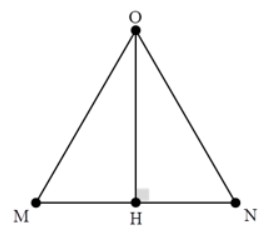
\includegraphics[scale=0.8]{../figs/VN12-PH-13-P-009-1-Q20.jpg}
	\end{center}
	
	Mức cường độ âm máy thu có thể thu được lớn nhất tại điểm H là hình chiếu của O lên MN.
	
	Ta có $\dfrac{\text{OH}}{\text{OM}}=\dfrac{\sqrt{3}}{2}$.
	
	Mức cường độ âm tại H là $L_\text{H}=L_\text{M}+20\log\dfrac{\text{OM}}{\text{OH}}=\SI{16}{dB}$
	

	
	
}
\end{enumerate}
\loigiai{\textbf{Đáp án}
	\begin{center}
		\begin{tabular}{|m{2.8em}|m{2.8em}|m{2.8em}|m{2.8em}|m{2.8em}|m{2.8em}|m{2.8em}|m{2.8em}|m{2.8em}|m{2.8em}|}
			\hline
			1. A & 2. C & 3. C & 4. C & 5. C & 6. A  & 7. B  & 8. D & 9. A & 10. A\\
			\hline
			11. C & 12. D & 13. B & 14. C & 15. D & 16. D  & 17. B  & 18. C & 19. A & 20. C\\
			\hline
		\end{tabular}
\end{center}}
\stopcontents[mychapters]
\setcounter{mychapter}{10}
\mychapter[Đặc trưng sinh lý của âm. Đồ thị dao động âm]{Đặc trưng sinh lý của âm.\\ Đồ thị dao động âm}
\startcontents[mychapters]
\printcontents[mychapters]{}{0}{\setcounter{tocdepth}{1}}
\begin{enumerate}[label=\bfseries Câu \arabic*:]
	
	\item \mkstar{1}

\cauhoi{
	
	Độ cao của âm
	\begin{mcq}(2)
		\item là một đặc trưng vật lý của âm.
		\item là một đặc trưng sinh lý của âm.
		\item vừa là đặc trưng sinh lý, vừa là đặc trưng vật lý.
		\item là tần số âm.
	\end{mcq}
}
\loigiai{
	\textbf{Đáp án B.}
	
	Độ cao của âm là một đặc trưng sinh lý của âm.
}
\item \mkstar{1}

\cauhoi{
	
	Độ cao của âm là đặc tính sinh lí của âm phụ thuộc vào
	\begin{mcq}(2)
		\item năng lượng âm.
		\item biên độ âm.
		\item vận tốc truyền âm.
		\item tần số âm.
	\end{mcq}
}
\loigiai{
	\textbf{Đáp án D.}
	
Độ cao của âm là đặc tính sinh lí của âm phụ thuộc vào tần số âm.
}
\item \mkstar{1}

\cauhoi{
	
	Độ to của âm là đặc tính sinh lí của âm phụ thuộc vào
	\begin{mcq}(2)
		\item cường độ âm.
		\item biên độ âm.
		\item vận tốc truyền âm.
		\item mức cường độ âm.
	\end{mcq}
}
\loigiai{
	\textbf{Đáp án D.}
	
	Độ to của âm là đặc tính sinh lí của âm phụ thuộc vào mức cường độ âm.
}
\item \mkstar{1}

\cauhoi{
	
	Âm do hai nhạc cụ khác nhau phát ra luôn khác nhau về
	\begin{mcq}(2)
		\item âm sắc.
		\item độ to.
		\item độ cao.
		\item cả độ cao, độ to lẫn âm sắc.
	\end{mcq}
}
\loigiai{
	\textbf{Đáp án A.}
	
	Âm do hai nhạc cụ khác nhau phát ra luôn khác nhau về âm sắc.
	
}
\item \mkstar{1}

\cauhoi{
	
	Chọn phát biểu \textbf{sai} khi nói về các đặc tính sinh lí của âm.
	\begin{mcq}
		\item Âm sắc gắn liền với tần số và mức cường độ âm.
		\item Có 3 đặc tính sinh lí: độ cao, độ to và âm sắc.
		\item Độ cao gắn liền với tần số nhưng không tỉ lệ.
		\item Độ to gắn liền với mức cường độ âm nhưng không tỉ lệ.
	\end{mcq}
}
\loigiai{
	\textbf{Đáp án A.}
	
	Âm sắc có liên quan mật thiết với đồ thị dao động âm.
	
}
\item \mkstar{2}

\cauhoi{
	
	Âm sắc là một đặc tính sinh lý của âm có thể giúp ta phân biệt được hai âm loại nào trong các loại dưới đây?
	\begin{mcq}
		\item Có cùng tần số phát ra bởi hai nhạc cụ khác nhau.
		\item Có cùng tần số phát ra trước hay sau bởi cùng một nhạc cụ.
		\item Có cùng biên độ phát ra trước hay sau bởi cùng một nhạc cụ.
		\item Có cùng biên độ phát ra bởi hai nhạc cụ khác nhau.
	\end{mcq}
}
\loigiai{
	\textbf{Đáp án A.}
	
	Âm sắc giúp ta phân biệt được âm cùng tần số phát ra từ hai nhạc cụ khác nhau.
}
\item \mkstar{2}

\cauhoi{
	
	Một sóng âm truyền trong không khí, trong số các đại lượng: biên độ sóng, tần số sóng, độ cao của âm và bước sóng; đại lượng không phụ thuộc vào các đại lượng còn lại là
	\begin{mcq}(2)
		\item bước sóng.
		\item biên độ sóng.
		\item độ cao của âm.
		\item tần số sóng.
	\end{mcq}
}
\loigiai{
	\textbf{Đáp án B.}
	
	Biên độ sóng không phụ thuộc và tần số, độ cao và bước sóng.
}
\item \mkstar{2}

\cauhoi{
	
	Độ trầm, bổng của âm liên quan mật thiết đến đặc trưng sinh lý nào của âm?
	\begin{mcq}(2)
		\item độ cao của âm.
		\item độ to của âm.
		\item cường độ của âm.
		\item âm sắc.
	\end{mcq}
}
\loigiai{
	\textbf{Đáp án A.}
	
Độ trầm, bổng của âm liên quan mật thiết đến độ cao của âm.

}
\item \mkstar{3}

\cauhoi{ 
	
	Trong âm nhạc, khoảng cách giữa hai nốt nhạc trong một quãng được tính bằng cung và nửa cung (nc). Mỗi quãng tám được chia thành 12 nc. Hai nốt nhạc cách nhau nửa cung thì hai âm (cao, thấp) tương ứng với hai nốt nhạc này có tần số thỏa mãn $f^{12}_c=2f^{12}_t$. Tập hợp tất cả các âm trong một quãng tám gọi là một gam (âm giai). Xét một gam với khoảng cách từ nốt Đồ đến các nốt tiếp theo Rê, Mi, Fa, Sol, La, Si, Đô tương ứng là 2 nc, 4 nc, 5 nc, 7 nc , 9 nc, 11 nc, 12 nc. Trong gam này, nếu âm ứng với nốt La có tần số $\SI{440}{Hz}$ thì âm ứng với nốt Sol có tần số là
	
	\begin{mcq}(4)
		\item $\SI{330}{Hz}$.
		\item $\SI{392}{Hz}$.
		\item $\SI{494}{Hz}$.
		\item $\SI{415}{Hz}$.
	\end{mcq}
}
\loigiai{
	\textbf{Đáp án B.}
	
	Khoảng cách giữa Son là La là 2 nc, nên âm ứng với nốt Sol có tần số là
	\begin{equation*}
		f^{12}_L=2\cdot2f^{12}_S=4f^{12}_S=f_S=\dfrac{f_L}{\sqrt[12]{4}}\approx\SI{392}{Hz}.
	\end{equation*}
	
}
\item \mkstar{3}

\cauhoi{	
	Một sóng hình sin đang truyền trên một sợi dây, theo chiều dương của trục Ox. Hình vẽ mô tả hình dạng của sợi dây ở các thời điểm $t_1$ và $t_2 = t_1 + 0,3\,\text{s}$.
	\begin{center}
		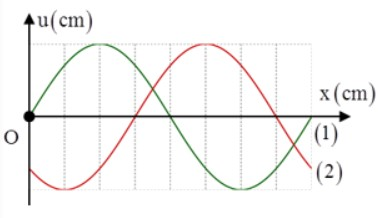
\includegraphics[scale=1.0]{../figs/dothisongco-h3.jpg}
	\end{center}
	Chu kì của sóng là
	\begin{mcq}(4)
		\item 0,9 s.
		\item 0,4 s.
		\item 0,6 s.
		\item 0,8 s.
	\end{mcq}
	
}

\loigiai{
	\textbf{Đáp án D.}
	
	Từ đồ thị dao đôngk sóng ta có:
	
	$$\Delta x = 3\ \text{ô} = \SI{3}{cm}; \lambda = 8\ \text{ô} = \SI{8}{cm}; \Delta t = \SI{0,3}{s}.$$
	

	
	Từ đồ thị ta thấy trong khoảng thời gian $\Delta t = 0,3\,\text{s}$, đỉnh sóng đi được quãng đường $S=3\,\text{cm}$
	
	Vận tốc truyền sóng $v=\dfrac{\Delta x}{\Delta t}=10\,\textrm{cm/s}$.
	
	Vậy chu kì của sóng: $T=\dfrac{\lambda}{v}=0,8\,\text{s}$.
	
}

%%%%%%%%%%%Câu 3%%%%%%%%%%%%%%
\item \mkstar{3}

\cauhoi{
	
	Một sóng hình sin truyền trên một sợ dây dài. Ở thời điểm $t$, hình dạng của một đoạn dây như hình vẽ. Các vị trí cân bằng của các phần tử trên dây cùng nằm trên trục O$x$.
	\begin{center}
		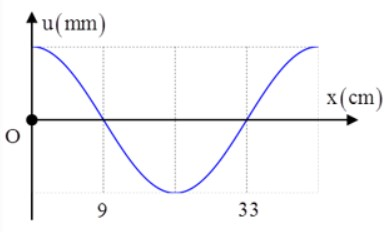
\includegraphics[scale=1.0]{../figs/dothisongco-h4.jpg}
	\end{center}
	Bước sóng của sóng này bằng
	\begin{mcq}(4)	
		\item 48 cm.
		\item 18 cm.
		\item 36 cm.
		\item 24 cm.
	\end{mcq}
	
}

\loigiai{
	\textbf{Đáp án A.}
	
	Từ hình vẽ ta có $\dfrac{\lambda}{2}=33-9=24\,\text{cm}\Rightarrow\lambda=48\,\text{cm}$.
}

%%%%%%%%%%%Câu 4%%%%%%%%%%%%%%
\item \mkstar{3} 

\cauhoi{	
	Hai điểm A, B cùng phương truyền sóng, cách nhau 25,5 cm. Trên đoạn AB có 3 điểm A$_1$, A$_2$, A$_3$ dao động cùng pha với A và 3 điểm B$_1$, B$_2$, B$_3$ dao động cùng pha với B. Sóng truyền theo thứ tự A, B$_1$, A$_1$, B$_2$, A$_2$, B$_3$, A$_3$ và A$_3$B = 3 cm.
	\begin{center}
		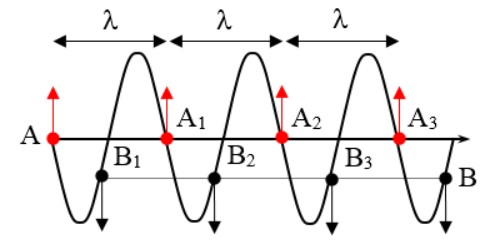
\includegraphics[scale=0.8]{../figs/dothisongco-h5.jpg}
	\end{center}
	Tìm bước sóng.
	\begin{mcq}(4)
		\item 6,5 cm.
		\item 7,5 cm.
		\item 5,5 cm.
		\item 4,5 cm.
	\end{mcq}
	
}

\loigiai{
	\textbf{Đáp án B.}
	
	Từ đồ thị ta có $\text{AB}=3\lambda+\text{A}_3\text{B}=3\lambda+3\Rightarrow25,5=3\lambda+3\Rightarrow\lambda=7,5\,\text{cm}$.
	
}

%%%%%%%%%%%Câu 5%%%%%%%%%%%%%%
\item \mkstar{3}

\cauhoi{
	Một sóng truyền theo phương AB. Tại một thời điểm nào đó, hình dạng sóng có dạng như hình vẽ. Biết rằng điểm M đang đi lên vị trí cân bằng. Khi đó điểm N đang chuyển động như thế nào?
	\begin{center}
		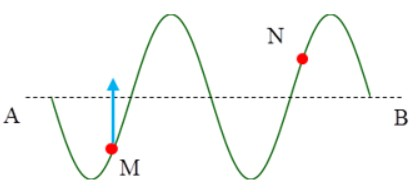
\includegraphics[scale=0.9]{../figs/dothisongco-h6.jpg}
	\end{center}
	\begin{mcq}(4)
		\item Đi xuống.
		\item Đứng yên.
		\item Chạy ngang.
		\item Đi lên.
	\end{mcq}
	
}

\loigiai{
	\textbf{Đáp án D.}
	
	\begin{center}
		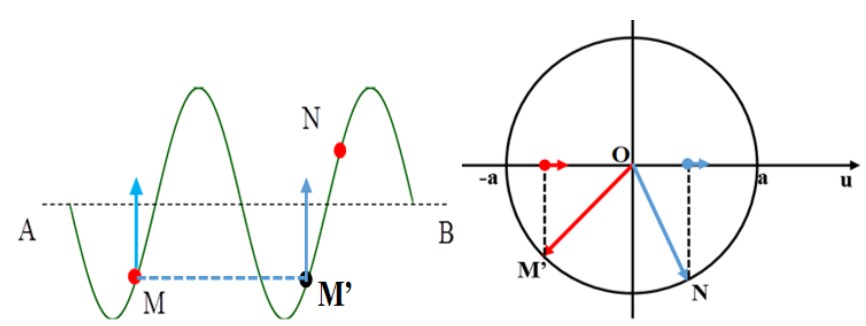
\includegraphics[scale=0.7]{../figs/dothisongco-h7.jpg}
	\end{center}
	
	Xét điểm M’ cách M một khoảng $d =\lambda$ (như hình vẽ) khi đó M’ cùng trạng thái với M (đang đi lên).
	
	Vì M’ lệch pha với N một góc $\Delta \varphi<\pi$, nên ta biểu diễn các vectơ quay như hình vẽ. Ta thấy N sớm pha hơn M’ và đang đi lên.
}
\item \mkstar{3}

\cauhoi{
	Một sóng ngang tần số 100 Hz truyền trên một sợi dây nằm ngang với vận tốc 60 m/s. M và N là hai điểm trên dây cách nhau 0,75 m và sóng truyền theo chiều từ M tới N. Chọn trục biểu diễn li độ cho các điểm có chiều dương hướng lên trên. Tại một thời điểm nào đó M có li độ âm và đang chuyển động đi xuống.
	\begin{center}
		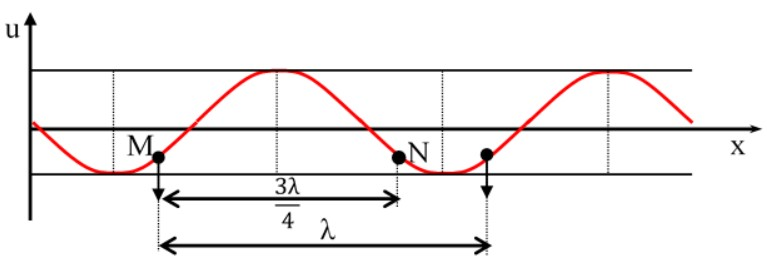
\includegraphics[scale=0.7]{../figs/dothisongco-h12.jpg}
	\end{center}
	Tại thời điểm đó N sẽ có li độ và chiều chuyển động tương ứng là
	\begin{mcq}(2)
		\item âm, đi xuống.
		\item âm, đi lên.
		\item dương, đi xuống.
		\item dương, đi lên.
	\end{mcq}	
	
}

\loigiai{
	\textbf{Đáp án C.}
	\begin{center}
		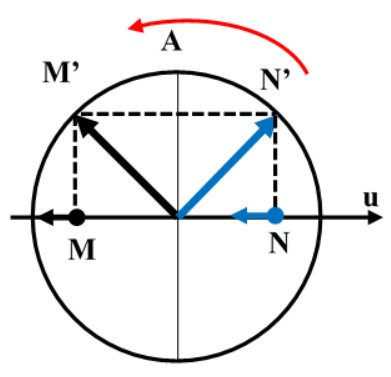
\includegraphics[scale=0.7]{../figs/dothisongco-h13.jpg}
	\end{center}
	Ta có: $\lambda=\dfrac{v}{f}=0,6\, \text{m}$.
	
	Theo giả thuyết: $\text{MN}=0,75=0,6+0,15=\lambda+\dfrac{\lambda}{4}$.
	
	Do sóng truyền từ M đến N nên dao động tại M sớm pha hơn dao động tại N một góc $$\Delta\varphi=\dfrac{2\pi d_\text{MN}}{\lambda}=2\pi+\dfrac{\pi}{2}.$$
	
	Dùng liên hệ giữa dao động điều hòa và chuyển động tròn đều.
	
	Ta thấy sóng truyền theo chiều từ M tới N, do đó M nhanh pha hơn N góc $\dfrac{\pi}{2}$. Lúc M có li độ âm và đang chuyển động đi xuống biên âm, thì N sẽ có li độ dương và đi xuống VTCB.
}

%%%%%%%%%%%Câu 9%%%%%%%%%%%%%%
\item \mkstar{3}

\cauhoi{
	
	Một sóng cơ truyền trên một sợi dây theo phương ngang, tốc độ truyền sóng là 20 cm/s. Tại thời điểm $t = 0$ hình dạng của sợi dây được biểu diễn như hình vẽ.
	\begin{center}
		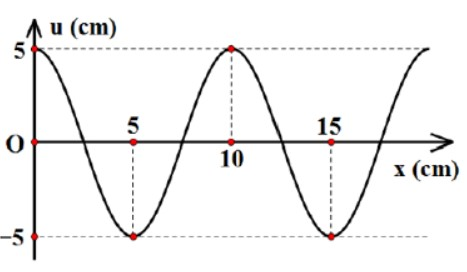
\includegraphics[scale=0.7]{../figs/dothisongco-h14.jpg}
	\end{center}
	Phương trình sóng cơ mô tả hình dáng của sợi dây tại thời điểm $t$ = 2,125 s là
	\begin{mcq}(2)
		\item $u = 5\cos(0,628x + 0,785)$ cm.
		\item $u = 5\cos(0,628x + 1,57)$ cm.
		\item $u = 5\cos(0,628x - 0,785)$ cm.
		\item $u = 5\cos(0,628x - 1,57)$ cm
	\end{mcq}
	
}

\loigiai{
	\textbf{Đáp án D.}
	
	Ta có: $\lambda=10\,\text{cm}\Rightarrow f=\dfrac{v}{\lambda}=2\,\text{Hz}\Rightarrow \omega=4\pi\, \text{rad/s}.$
	
	Tại thời điểm $t$ = 2,125 s phương trình sóng của sợi dây là
	$$u=5\cos\left(\omega t-\dfrac{2\pi x}{\lambda}\right)=5\cos(0,628x - 1,57)\,\text{cm}.$$
	
}
%%%%%%%%%%%Câu 10%%%%%%%%%%%%%%
\item \mkstar{4}

\cauhoi{	
	Một sóng ngang hình sin truyền trên một sợi dây dài. Hình vẽ bên là hình dạng của một đoạn dây tại một thời điểm xác định.
	\begin{center}
		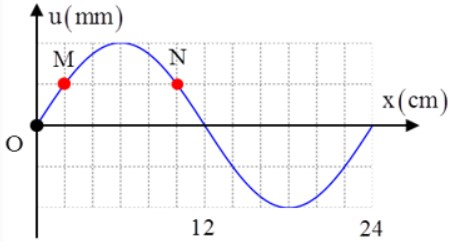
\includegraphics[scale=0.8]{../figs/dothisongco-h15.jpg}
	\end{center}
	Trong quá trình lan truyền sóng, khoảng cách lớn nhất giữa hai phần tử M và N có giá trị gần với giá trị nào sau đây? 
	\begin{mcq}(4)
		\item $8,35\,\text{cm}$.
		\item $8,2\,\text{cm}$.
		\item $8,5\,\text{cm}$.
		\item $8,05\,\text{cm}$.
	\end{mcq}
}

\loigiai{
	\textbf{Đáp án: B}
	
	Dựa vào đồ thị, ta thấy bước sóng $\lambda=24\,\textrm{cm}$ và biên độ sóng $A=1\,\textrm{cm}$.
	
	Dễ thấy mỗi ô chữ nhật có độ dài $2\,\textrm{cm}$, suy ra $\text{MN}=8\,\textrm{cm}$.
	
	Độ lệch pha giữa hai điểm cách nhau một khoảng $d$ theo phương truyền sóng $$\Delta \varphi=\dfrac{2 \pi d}{\lambda}=\frac{2 \pi \cdot 8}{24}=\frac{2 \pi}{3}\, \mathrm{rad}.$$
	
	Khoảng cách giữa hai điểm M, N là $d=\text{MN}=8\,\textrm{cm}$ $$d=\sqrt{8^2+(\sqrt{3})^2}=8,2\,\text{cm}.$$
	
}
\item \mkstar{4}

\cauhoi{
	Ở Việt Nam, phổ biến loại sáo trúc có 6 lỗ bấm, 1 lỗ thổi và một lỗ định âm (là lỗ để sáo phát ra âm cơ bản). Các lỗ bấm đánh số 1, 2, 3, 4, 5, 6 tính từ lỗ định âm; các lỗ này phát ra các âm có tần số cách âm cơ bản được tính bằng cung theo thứ tự; 1 cung, 2 cung, 2,5 cung, 3,5 cung, 4,5 cung, 5,5 cung. Coi rằng mỗi lỗ bấm là một ống sáo rút ngắn. Hai lỗ cách nhau một cung và nửa cung (tính từ lỗ định âm) thì có tỉ số chiều dài đến lỗ thổi tương ứng là $\dfrac{8}{9}$ và $\dfrac{15}{16}$ . Giữa chiều dài L, từ lỗ thổi đến lỗ thứ i và tần số $f_i$ ($i=1\rightarrow 6$) của âm phát ra từ lỗ đó tuân theo công thức $L = \dfrac{v}{2f_1}$ ($v$ là tốc độ truyền âm trong không khí bằng $\SI{340}{\meter/\second}$). Một ống sáo phát ra âm cơ bản có tần số $f_0=\SI{440}{Hz}$. Lỗ thứ 5 phát ra âm cơ bản có tần số
	\begin{mcq}(4)
		\item $\SI{392}{Hz}$.
		\item $\SI{494}{Hz}$.
		\item $\SI{751.8}{Hz}$.
		\item $\SI{257.5}{Hz}$.
	\end{mcq}
	
}
\loigiai{
	\textbf{Đáp án C.}
	
	
	\begin{center}
		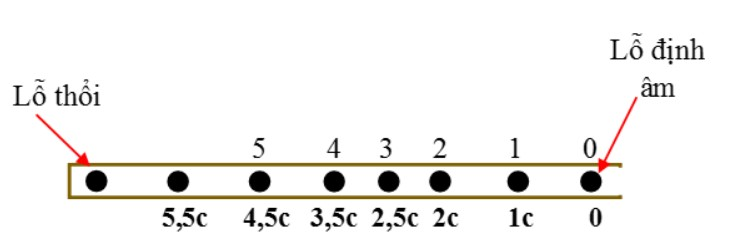
\includegraphics[scale=0.7]{../figs/VN12-PH-14-L-009-2-1.jpg}
	\end{center}
	Gọi khoảng cách các lỗ 0, 1, 2, 3, 4, 5 đến lỗ thổi lần lượt là $L_0$, $L_1$, $L_2$, $L_3$, $L_4$, $L_5$.
	
	Ta có:
	\begin{equation*}
		\dfrac{L_5}{L_0}=\dfrac{L_5}{L_4}\cdot\dfrac{L_4}{L_3}\cdot\dfrac{L_3}{L_2}\cdot\dfrac{L_2}{L_1}\cdot\dfrac{L_1}{L_0}=\dfrac{8}{9}\cdot\dfrac{8}{9}\cdot\dfrac{15}{16}\cdot\dfrac{8}{9}\cdot\dfrac{8}{9}=\dfrac{1280}{2187}.
	\end{equation*}
	
	Mặt khác:
	\begin{equation*}
		\dfrac{L_5}{L_0}=\dfrac{f_0}{f_5}\Rightarrow f_5=f_0\cdot\dfrac{L_0}{L_5}=\SI{440}{Hz}\cdot\dfrac{2187}{1280}\approx\SI{751.8}{Hz}.
	\end{equation*}
	
	Vậy lỗ thứ 5 phát ra âm cơ bản có tần số $\SI{751.8}{Hz}$.
	
}
	\item \mkstar{4}	

\cauhoi{		
	Trên một sợ dây dài, đang có sóng ngang hình sin truyền qua theo chiều dương của trục O$x$. Tại thời điểm $t_0$ một đoạn của sợi dây có hình dạng như hình bên.
	\begin{center}
		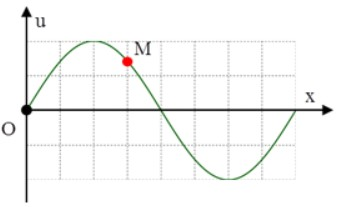
\includegraphics[scale=1.0]{../figs/dothisongco-h1.jpg}
	\end{center}
	Hai phần tử M và O dao động lệch pha nhau	
	\begin{mcq}(4)
		\item $\dfrac{\pi}{4}$ rad.
		\item $\dfrac{\pi}{3}$ rad.
		\item $\dfrac{3\pi}{4}$ rad.
		\item $\dfrac{2\pi}{3}$ rad.
	\end{mcq}		
}

\loigiai{
	\textbf{Đáp án C.}
	
	\begin{center}
		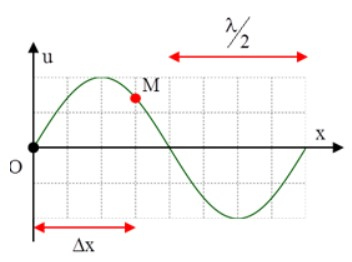
\includegraphics[scale=1.0]{../figs/dothisongco-h2.jpg}
	\end{center}
	
	Từ hình vẽ ta có $\Delta x=3\textrm{ ô đơn vị}$ và $\lambda=8\textrm{ ô đơn vị}$ nên $\dfrac{\Delta x}{\lambda}=\dfrac{3}{8}$.
	
	Vậy độ lệch pha giữa hai điểm O và M là $\Delta \varphi=\dfrac{2\pi \Delta x}{\lambda}=\dfrac{3\pi}{4}\,\text{rad}$.
	
}

%%%%%%%%%%%Câu 2%%%%%%%%%%%%%%


%%%%%%%%%%%Câu 6%%%%%%%%%%%%%%
\item \mkstar{4}

\cauhoi{	
	Một sóng cơ học tại thời điểm $t = 0$ có đồ thị là đường liền nét. Sau thời gian $t$, nó có đồ thị là đường đứt nét. Cho biết vận tốc truyền sóng là 4 m/s, sóng truyền từ phải qua trái. Giá trị của $t$ là
	\begin{center}
		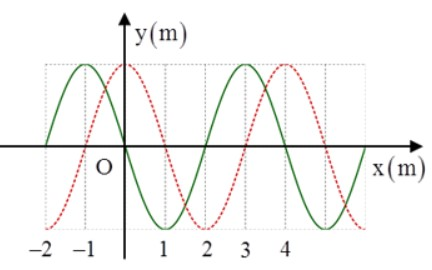
\includegraphics[scale=0.8]{../figs/dothisongco-h8.jpg}
	\end{center}	
	\begin{mcq}(4)
		\item 0,25 s.
		\item 1,25 s.
		\item 0,75 s.
		\item 2,5 s.
	\end{mcq}
	
}

\loigiai{
	\textbf{Đáp án C.}
	
	\begin{center}
		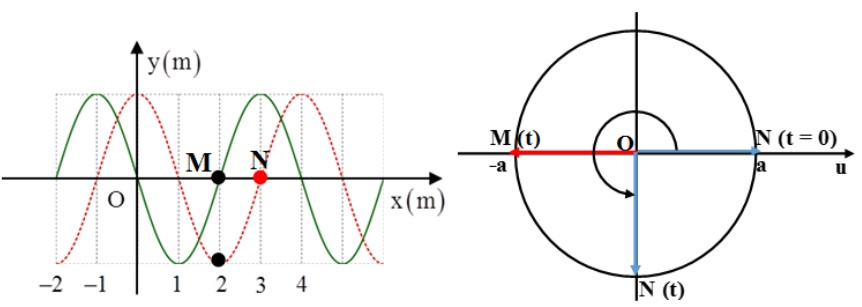
\includegraphics[scale=0.8]{../figs/dothisongco-h9.jpg}
	\end{center}
	
	Chọn hai điểm M, N trên phương truyền sóng, cách nhau $d=\dfrac{\lambda}{4}$ như hình vẽ, độ lệch pha của M, N là $\dfrac{\pi}{2}$.
	
	Vì sóng truyền từ phải qua trái nên N sớm pha hơn M.
	
	Tại thời điểm $t = 0$ thì N ở biên dương, M ở VTCB.
	
	Tại thời điểm $t$, N ở VTCB, M ở biên âm.
	
	Trên vòng tròn lượng giác ta nhận thấy góc quét từ thời điểm $t = 0$ đến $t$ là $\dfrac{3\pi}{2}$.
	
	Do đó: $t=\dfrac{3T}{4}$.
	
	Chu kì của sóng: $T=\dfrac{\lambda}{v}=1\,\text{s}\Rightarrow t=0,75\,\text{s}$.
}

%%%%%%%%%%%Câu 7%%%%%%%%%%%%%%
\item \mkstar{4}

\cauhoi{
	
	Sóng truyền trên một sợi dây đàn hồi theo ngược chiều dương trục O$x$. Tại một thời điểm nào đó thì hình dạng sợi dây được cho như hình vẽ. Các điểm O, M, N nằm trên dây. Chọn đáp án đúng.
	\begin{center}
		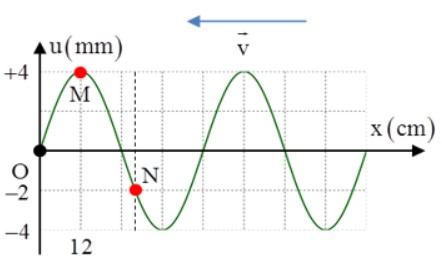
\includegraphics[scale=0.8]{../figs/dothisongco-h10.jpg}
	\end{center}
	\begin{mcq}(2)
		\item ON = 30cm, N đang đi lên.
		\item ON = 28cm, N đang đi lên.
		\item ON = 30cm, N đang đi xuống.
		\item ON = 28cm, N đang đi xuống.
	\end{mcq}
	
}

\loigiai{
	\textbf{Đáp án D.}
	
	\begin{center}
		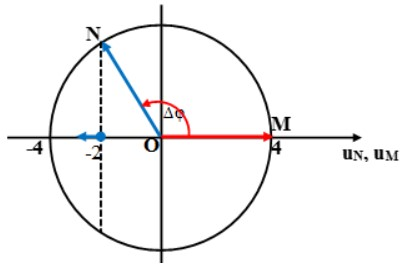
\includegraphics[scale=0.8]{../figs/dothisongco-h11.jpg}
	\end{center}
	
	Từ đồ thị ta có: $\text{OM}=12\,\text{cm}=\dfrac{\lambda}{4}\Rightarrow\lambda=48\,\text{cm}$
	
	Theo phương truyền sóng, so sánh với đỉnh gần nhất. Trước đỉnh sóng thì phần tử môi trường đi xuống, sau đỉnh sóng thì phần tử môi trường đi lên, suy ra N trước đỉnh M sẽ đi xuống.
	
	(Hoặc sử dụng vòng tròn lượng giác để biểu diễn dao động phần tử sóng tại M, N với điều kiện sóng truyền từ N sang M nên N phải sớm pha hơn M).
	
	Từ hình vẽ ta thấy điểm N có li độ $u_\text{N}=-2=\dfrac{-A_\text{M}}{2}$.
	
	Do đó
	$$\Delta\varphi=\dfrac{2\pi d_\text{MN}}{\lambda}=\dfrac{2\pi}{3}\Rightarrow d_\text{MN}=\dfrac{\lambda}{3}=16\,\text{cm}.$$
	
	Vậy ON = OM + MN = 12 + 16 = 28 cm.
	
}
%%%%%%%%%%%Câu 8%%%%%%%%%%%%%%

\end{enumerate}
\loigiai{\textbf{Đáp án}
	\begin{center}
		\begin{tabular}{|m{2.8em}|m{2.8em}|m{2.8em}|m{2.8em}|m{2.8em}|m{2.8em}|m{2.8em}|m{2.8em}|m{2.8em}|m{2.8em}|}
			\hline
			1. B & 2. D & 3. D & 4. A & 5. A & 6. A  & 7. B  & 8. A & 9. B & 10. D\\
			\hline
				11. A & 12. B & 13. D & 14. C & 15. D & 16. B  & 17. C  & 18. C & 19. C & 20. D\\
			\hline
		\end{tabular}
\end{center}}
\stopcontents[mychapters]
\chapter{Ôn tập: Chương II. Sóng cơ và sóng âm}
\begin{enumerate}[label=\bfseries Câu \arabic*:]
	\item \mkstar{1}
	
	\cauhoi{
		Chọn phát biểu \textbf{sai} khi nói về môi trường truyền âm và vận tốc âm.
		
		\begin{mcq}
			\item Môi trường truyền âm có thể là rắn, lỏng hoặc khí.
			\item Những vật liệu như bông, nhung, xốp truyền âm tốt.
			\item Vận tốc truyền âm phụ thuộc vào tính đàn hồi và mật độ của môi trường.
			\item Vận tốc truyền âm phụ thuộc vào nhiệt độ của môi trường.
		\end{mcq}
	}
	\loigiai{
		\textbf{Đáp án B.}
		
	}
	
	\item \mkstar{1}
	
	\cauhoi{
		Khi sóng âm truyền từ môi trường không khí vào môi trường nước thì
		
		\begin{mcq}(2)
			\item chu kì tăng.
			\item tần số không đổi.
			\item bước sóng giảm.
			\item bước sóng không đổi.
		\end{mcq}
	}
	\loigiai{
		\textbf{Đáp án B.}
		
	}
	
	\item \mkstar{1}
	
	\cauhoi{
		Khi nói về sóng cơ, phát biểu nào sau đây \textbf{sai}?
		
		\begin{mcq}
			\item Sóng âm truyền trong không khí là sóng dọc.
			\item Sóng cơ học lan truyền trên mặt nước là sóng ngang.
			\item Sóng cơ học là sự lan truyền dao động cơ học trong môi trường vật chất.
			\item Sóng cơ học truyền được trong môi trường rắn, lỏng, khí và chân không.
		\end{mcq}
	}
	\loigiai{
		\textbf{Đáp án D.}
		
		Sóng cơ học truyền được trong môi trường rắn, lỏng, khí. Sóng cơ học không truyền được trong chân không.
	}
	
	\item \mkstar{1}
	
	\cauhoi{
		Chọn phát biểu \textbf{sai} khi nói về sóng âm.
		
		\begin{mcq}
			\item Tai người không nghe được sóng âm có tần số nhỏ hơn $\SI{16}{Hz}$ hoặc lớn hơn $\SI{20}{Hz}$.
			\item Các đặc trưng sinh lý của âm là độ cao, độ to và âm sắc.
			\item Tần số âm là một trong những đặc trưng vật lý của âm.
			\item Độ cao của âm phụ thuộc vào tần số âm.
		\end{mcq}
	}
	\loigiai{
		\textbf{Đáp án A.}
		
		Tai người không thể nghe được các âm có tần số lớn hơn $\SI{20}{kHz}$, không phải $\SI{20}{Hz}$.
	}
	
	\item \mkstar{1}
	
	\cauhoi{
		Chọn ý \textbf{sai}. Hộp đàn có tác dụng
		
		\begin{mcq}(2)
			\item làm cho âm phát ra cao hơn.
			\item làm cho âm phát ra to hơn.
			\item như hộp cộng hưởng âm.
			\item làm cho âm phát ra có âm sắc riêng.
		\end{mcq}
	}
	\loigiai{
		\textbf{Đáp án A.}
		
		Hộp đàn có tác dụng như hộp cộng hưởng âm, làm cho cho âm phát ra to hơn và làm cho âm phát ra có âm sắc riêng.
	}
	
	\item \mkstar{1}
	
	\cauhoi{
		Đặc điểm nào sau đây \textbf{không} phải của sóng cơ?
		\begin{mcq}
			\item Sóng cơ có thể giao thoa, phản xạ, nhiễu xạ.
			\item Sóng cơ truyền trong chất khí nhanh hơn truyền trong chất rắn.
			\item Sóng dọc có phương dao động trùng với phương truyền sóng.
			\item Sóng cơ không lan truyền được trong chân không.
		\end{mcq}
	}
	\loigiai{
		\textbf{Đáp án B.}
		
		Sóng cơ truyền trong chất khí chậm hơn truyền trong chất lỏng, truyền trong chất lỏng chậm hơn truyền trong chất rắn.
	}
	
	\item \mkstar{2}
	
	\cauhoi{
		Một lá thép mỏng, một đầu cố định, đầu còn lại được kích thích để dao động với chu kì không đổi và bằng $\SI{0.008}{s}$. Cho rằng cường độ âm đủ lớn. Âm do lá thép phát ra là
		
		\begin{mcq}(2)
			\item âm không nghe được.
			\item hạ âm.
			\item âm nghe được.
			\item siêu âm.
		\end{mcq}
	}
	\loigiai{
		\textbf{Đáp án C.}
		
		Tần số của âm:
		$$f=\dfrac{1}{T} = \SI{125}{Hz}.$$
		
		Đây là tần số âm mà tai người có thể nghe được.
	}
	
	\item \mkstar{2}
	
	\cauhoi{
		Hai nhạc cụ 1 và 2 phát ra hai âm có đồ thị dao động $x_1-t$ và $x_2-t$ như hình vẽ.
		\begin{center}
			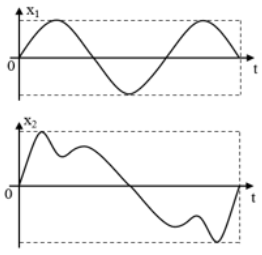
\includegraphics[scale=1.2]{../figs/VN12-2021-PH-TP015-1}
		\end{center}
		
		Chọn phát biểu đúng.
		\begin{mcq}(2)
			\item Độ cao của âm 1 lớn hơn âm 2.
			\item Hai âm có cùng âm sắc.
			\item Hai âm có cùng tần số.
			\item Độ cao của âm 2 lớn hơn âm 1.
		\end{mcq}
	}
	\loigiai{
		\textbf{Đáp án A.}
		
		Chu kì của âm 2 lớn hơn âm 1 nên tần số của âm 1 lớn hơn âm 2. Vậy độ cao của âm 1 lớn hơn âm 2.
	}
	
	\item \mkstar{2}
	
	\cauhoi{
		Dao động của sóng cơ tại một điểm trên mặt chất lỏng có phương trình là $u=A \cos (20x - 2000t)$, với $x$ đo bằng mét, $t$ đo bằng giây. Tốc độ truyền sóng trên mặt chất lỏng là
		
		\begin{mcq}(4)
			\item $\SI{200}{m/s}$.
			\item $\SI{20}{m/s}$.
			\item $\SI{100}{m/s}$.
			\item $\SI{10}{m/s}$.
		\end{mcq}
	}
	\loigiai{
		\textbf{Đáp án C.}
		
		Phương trình sóng tại một điểm có dạng tổng quát:
		$$u= A \cos \left(\omega t - \dfrac{2\pi d}{\lambda}\right)$$
		
		So sánh với phương trình $u=A \cos (20x - 2000 t) = A \cos (2000t - 20x)$, ta có:
		$$20=\dfrac{2\pi}{\lambda} \Rightarrow \lambda = \dfrac{\pi}{10}\ \text{m}.$$
		$$\omega = \SI{2000}{rad/s}.$$
		
		Vậy tốc độ truyền sóng là
		$$v=\lambda f = \lambda \dfrac{\omega}{2\pi} = \SI{100}{m/s}.$$
	}
	
	\item \mkstar{2}
	
	\cauhoi{
		Một sóng có tần số $\SI{100}{Hz}$ truyền trong một môi trường với tốc độ $\SI{50}{m/s}$. Bước sóng của sóng này là
		
		\begin{mcq}(4)
			\item $\SI{0.25}{m}$.
			\item $\SI{1.0}{m}$.
			\item $\SI{0.75}{m}$.
			\item $\SI{0.5}{m}$.
		\end{mcq}
	}
	\loigiai{
		\textbf{Đáp án D.}
		
		Bước sóng của sóng này là
		$$\lambda = \dfrac{v}{f} = \SI{0.5}{m}.$$
	}
	
	\item \mkstar{2}
	
	\cauhoi{
		Cho hai nguồn sóng kết hợp $\text{S}_1$, $\text{S}_2$ giống hệt nhau, cách nhau $\SI{5}{cm}$. Sóng do hai nguồn này tạo ra có bước sóng $\SI{2}{cm}$. Trên đoạn $\text{S}_1 \text{S}_2$ quan sát được số cực đại giao thoa là
		
		\begin{mcq}(4)
			\item 7.
			\item 5.
			\item 9.
			\item 3.
		\end{mcq}
	}
	\loigiai{
		\textbf{Đáp án B.}
		
		Điều kiện xảy ra cực đại giao thoa:
		$$- \dfrac{\text{S}_1 \text{S}_2}{\lambda} \leq k \leq \dfrac{\text{S}_1 \text{S}_2}{\lambda} \Rightarrow \SI{-2.5}{} \leq k \leq \SI{2.5}{}$$
		
		Vậy có 5 điểm thỏa mãn.
	}
	
	\item \mkstar{2}
	
	\cauhoi{
		Một sóng cơ học lan truyền dọc theo trục O$x$ có phương trình $u=12 \cos (20t - 4x)\ \text{cm}$, trong đó $x$ là tọa độ tính bằng mét, $t$ là thời gian được tính bằng giây. Tốc độ truyền sóng là
		
		\begin{mcq}(4)
			\item $\SI{5}{m/s}$.
			\item $\SI{0.5}{m/s}$.
			\item $\SI{40}{m/s}$.
			\item $\SI{4}{m/s}$.
		\end{mcq}
	}
	\loigiai{
		\textbf{Đáp án A.}
		
		Tần số sóng:
		$$f=\dfrac{\omega}{2\pi} = \xsi{\dfrac{10}{\pi}}{Hz}.$$
		
		Bước sóng:
		$$-\dfrac{2\pi}{\lambda} = -4 \Rightarrow \lambda = \dfrac{\pi}{2}\ \text{m}$$
		
		Tốc độ truyền sóng:
		$$v=\lambda f = \SI{5}{m/s}$$
	}
	
	\item \mkstar{2}
	
	\cauhoi{
		Một sóng có tần số $\SI{500}{Hz}$ lan truyền với tốc độ $\SI{350}{m/s}$. Hai điểm gần nhau nhất trên cùng một phương truyền sóng phải cách nhau một khoảng là bao nhiêu để chúng có độ lệch pha là $\dfrac{\pi}{3}\ \text{rad}$?
		
		\begin{mcq}(4)
			\item $\SI{4.285}{m}$.
			\item $\SI{0.233}{m}$.
			\item $\SI{0.476}{m}$.
			\item $\SI{0.116}{m}$.
		\end{mcq}
	}
	\loigiai{
		\textbf{Đáp án D.}
		
		Bước sóng:
		$$\lambda = \dfrac{v}{f} = \SI{0.7}{m}.$$
		
		Độ lệch pha:
		$$\Delta \varphi = \dfrac{2\pi}{\lambda} x = \dfrac{\pi}{3} \Rightarrow \dfrac{2}{\lambda} x = \dfrac{1}{3} \Rightarrow x = \SI{0.116}{m}.$$
	}
	
	\item \mkstar{2}
	
	\cauhoi{
		Một người quan sát trên mặt biển nhận thấy trong $\SI{4}{s}$ có 3 ngọn sóng biển đi qua trước mặt mình, khoảng cách giữa hai ngọn sóng liên tiếp là $\SI{12}{cm}$. Tốc độ truyền sóng trên mặt biển là
		
		\begin{mcq}(4)
			\item $\SI{24}{cm/s}$.
			\item $\SI{12}{cm/s}$.
			\item $\SI{6}{cm/s}$.
			\item $\SI{18}{cm/s}$.
		\end{mcq}
	}
	\loigiai{
		\textbf{Đáp án C.}
		
		Bước sóng: $\lambda = \SI{12}{cm}$.
		
		Chu kì: $2T = \SI{4}{s} \Rightarrow T = \SI{2}{s}$.
		
		Tốc độ truyền sóng:
		$$v=\dfrac{\lambda}{T} = \SI{6}{cm/s}.$$
	}
	
	\item \mkstar{2}
	
	\cauhoi{
		Người ta làm cho đầu O của một sợi dây căng ngang dao động điều hòa theo phương vuông góc với sợi dây, với chu kì $\SI{1.2}{s}$. Sau $\SI{3}{s}$, sóng truyền được $\SI{12}{m}$ theo chiều dài sợi dây. Bước sóng của sóng truyền trên dây là
		
		\begin{mcq}(4)
			\item $\SI{4}{m}$.
			\item $\SI{3.6}{m}$.
			\item $\SI{0.3}{m}$.
			\item $\SI{4.8}{m}$.
		\end{mcq}
	}
	\loigiai{
		\textbf{Đáp án D.}
		
		Vận tốc truyền sóng:
		$$v=\dfrac{s}{t} = \SI{4}{m/s}.$$
		
		Bước sóng:
		$$\lambda = vT = \SI{4.8}{m}.$$
	}
	
	\item \mkstar{2}
	
	\cauhoi{
		Hiệu số pha của hai sóng kết hợp, đồng pha truyền tới một điểm có giá trị nào sau đây để khi giao thoa, biên độ sóng có giá trị cực tiểu?
		
		\begin{mcq}(4)
			\item $\dfrac{\pi}{4}\ \text{rad}$.
			\item $\pi\ \text{rad}$.
			\item $\dfrac{\pi}{2}\ \text{rad}$.
			\item $0\ \text{rad}$.
		\end{mcq}
	}
	\loigiai{
		\textbf{Đáp án B.}
		
		Biên độ sóng khi giao thoa có giá trị cực tiểu khi $d_2 - d_1 = \xsi{\pi}{rad}$.
	}
	
	\item \mkstar{2}
	
	\cauhoi{
		Một sợi dây có chiều dài $l$ được giữ cố định ở hai đầu. Âm do dây phát ra có bước sóng lớn nhất bằng
		
		\begin{mcq}(4)
			\item $2l$.
			\item $\dfrac{l}{2}$.
			\item $l$.
			\item $\dfrac{l}{4}$.
		\end{mcq}
	}
	\loigiai{
		\textbf{Đáp án A.}
		
		Điều kiện xảy ra sóng dừng trên dây có hai đầu cố định:
		$$l=k \dfrac{\lambda}{2} \Rightarrow \lambda = \dfrac{2l}{k}.$$
		
		Bước sóng lớn nhất khi $k=1$, khi đó $\lambda = 2l$.
	}
	
	\item \mkstar{2}
	
	\cauhoi{
		Tại điểm O trên mặt nước có dao động điều hòa với chu kì $\SI{0.4}{s}$. Tốc độ truyền sóng trên mặt nước là $v=\SI{60}{cm/s}$. Khoảng cách từ đỉnh sóng thứ 2 đến đỉnh sóng thứ 6 kể từ O, trên cùng một phương chiều truyền sóng là
		
		\begin{mcq}(4)
			\item $\SI{96}{cm}$.
			\item $\SI{120}{cm}$.
			\item $\SI{24}{cm}$.
			\item $\SI{48}{cm}$.
		\end{mcq}
	}
	\loigiai{
		\textbf{Đáp án A.}
		
		Bước sóng:
		$$\lambda = vT = \SI{24}{cm}.$$
		
		Khoảng cách từ đỉnh sóng thứ 2 đến đỉnh sóng thứ 6: $4\lambda = \SI{96}{cm}$.
	}
	
	\item \mkstar{2}
	
	\cauhoi{
		Một nguồn đặt tại O phát ra sóng cơ có bước sóng bằng $\SI{10}{m}$ và biên độ $\SI{2}{cm}$. Chọn gốc thời gian là lúc nguồn ở vị trí cân bằng và bắt đầu chuyển động theo chiều dương. Biết tốc độ truyền sóng là $\SI{5}{m/s}$. Phương trình dao động tại một điểm M cách O một khoảng $\SI{2.5}{cm}$ theo phương truyền sóng là
		
		\begin{mcq}(2)
			\item $u_\text{M} = 2 \cos (\pi t + \pi)\ \text{cm}$.
			\item $u_\text{M} = 2 \cos \left(\pi t - \dfrac{\pi}{2}\right)\ \text{cm}$.
			\item $u_\text{M} = 2 \cos (2\pi t + \pi)\ \text{cm}$.
			\item $u_\text{M} = 2 \cos \left(2 \pi t - \dfrac{\pi}{2}\right)\ \text{cm}$.
		\end{mcq}
	}
	\loigiai{
		\textbf{Đáp án A.}
		
		Ta có: $\lambda = vT \Rightarrow T = \dfrac{\lambda}{v} = \SI{2}{s} \Rightarrow \omega = \dfrac{2\pi}{T} = \xsi{\pi}{rad/s}$.
		
		Phương trình sóng tại O:
		$$u_\text{O} = A \cos \left(\pi t - \dfrac{\pi}{2}\right)\ \text{cm}.$$
		
		Phương trình sóng tại M:
		$$u_\text{M} = A \cos (\pi t - \dfrac{\pi}{2} - \dfrac{2\pi d}{\lambda}).$$
		
		Mà $d=\SI{2.5}{m}$, suy ra: $\dfrac{2\pi d}{\lambda} = \dfrac{\pi}{2}\ \text{rad}$. Vậy:
		$$u_\text{M} = 2 \cos (\pi t + \pi)\ \text{cm}.$$
	}
	
	\item \mkstar{2}
	
	\cauhoi{
		Để đo độ sâu của vực sâu nhất thế giới (Mariana ở Thái Bình Dương), người ta dùng phương pháp định vị hồi âm bằng sóng siêu âm. Sau khi phát ra siêu âm hướng xuống biển thì sau $\SI{14.53}{s}$ người ta mới nhận được tín hiệu phản xạ của nó từ đáy biển. Vận tốc truyền âm của siêu âm trong nước biển là $\SI{1500}{m/s}$, trong không khí là $\SI{340}{m/s}$. Độ sâu của vực Mariana đo được là
		
		\begin{mcq}(4)
			\item $\SI{2470.1}{m}$.
			\item $\SI{4940.2}{m}$.
			\item $\SI{21795.5}{m}$.
			\item $\SI{10897.5}{m}$.
		\end{mcq}
	}
	\loigiai{
		\textbf{Đáp án D.}
		
		Vì sóng âm truyền từ mặt biển xuống đáy vực rồi phản xạ từ đáy vực lên mặt biển, nên quãng đường sóng truyền bằng 2 lần độ sâu vực:
		$$2d = vt \Rightarrow d = \SI{10897.5}{m}.$$
	}
	
	\item \mkstar{3}
	
	\cauhoi{
		Trên mặt thoáng của một chất lỏng, một mũi nhọn O chạm vào mặt nước dao động điều hòa với tần số $f$ tạo thành sóng trên mặt thoáng với bước sóng $\lambda$. Xét trên hai phương truyền sóng O$x$ và O$y$ vuông góc với nhau. Gọi A là điểm thuộc O$x$ cách O một đoạn $16 \lambda$ và B là điểm thuộc O$y$ cách O một đoạn $12\lambda$. Tìm số điểm dao động ngược pha với nguồn trên đoạn AB.
		
		\begin{mcq}(4)
			\item 8 điểm.
			\item 9 điểm.
			\item 6 điểm.
			\item 12 điểm.
		\end{mcq}
	}
	\loigiai{
		\textbf{Đáp án A.}
		
		Ta có: $\text{AB} = \sqrt{\text{OA}^2 + \text{OB}^2} = 20 \lambda$.
		
		Để một điểm ngược pha với nguồn thì $d=k \lambda$, với $k$ là số bán nguyên.
		
		Áp dụng hệ thức lượng, ta có $\text{OH} = \SI{9.6}{}\lambda$.
		\begin{center}
			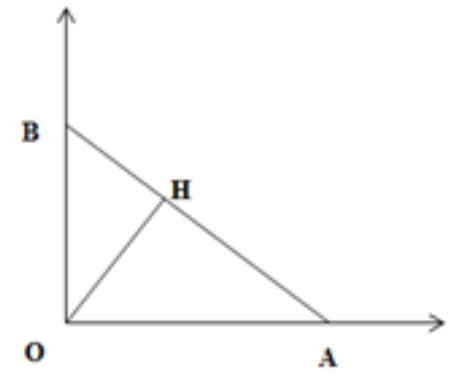
\includegraphics[scale=0.8]{../figs/VN12-2021-PH-TP015-5}
		\end{center}
	
		Số điểm nằm trên đoạn AH ngược pha với nguồn:
		$$\text{OH} \leq d \leq \text{OA} \Rightarrow k = \SI{10.5}{};\ \SI{11.5}{};\ \SI{12.5}{};\ \SI{13.5}{};\ \SI{14.5}{};\ \SI{15.5}{}.$$
		
		Số điểm nằm trên đoạn BH ngược pha với nguồn:
		$$\text{OH} \leq d \leq \text{OB} \Rightarrow k = \SI{10.5}{};\ \SI{11.5}{}.$$
		
		Vậy có tổng cộng 8 điểm thỏa mãn yêu cầu.
	}
	
	\item \mkstar{3}
	
	\cauhoi{
		Tại O có một nguồn phát sóng cơ với tần số $f=\SI{20}{Hz}$, tốc độ truyền sóng là $\SI{60}{cm/s}$. Ba điểm thẳng hàng A, B, C nằm trên cùng phương truyền sóng và cùng phía so với O. Biết $\text{OA} = \SI{8}{cm}$, $\text{OB} = \SI{25.5}{cm}$, $\text{OC} = \SI{40.5}{cm}$. Số điểm dao động cùng pha với A trên đoạn BC là
		
		\begin{mcq}(4)
			\item 3 điểm.
			\item 5 điểm.
			\item 4 điểm.
			\item 6 điểm.
		\end{mcq}
	}
	\loigiai{
		\textbf{Đáp án B.}
		
		Bước sóng:
		$$\lambda = \dfrac{v}{f} = \SI{3}{cm}.$$
		
		Để M nằm giữa BC và cùng pha với A thì:
		$$d_\text{M} - d_\text{A} = k\lambda \Rightarrow d_\text{M} = 8 + 3k\ (k \in \mathbb{Z}).$$
		
		Áp điều kiện:
		$$\SI{25.5}{cm} \leq 8 + 3k \leq \SI{40.5}{cm} \Rightarrow k = 6;\ 7;\ 8;\ 9;\ 10.$$
		
		Có 5 điểm thỏa mãn.
	}
	
	\item \mkstar{3}
	
	\cauhoi{
		Khi cường độ âm tăng gấp 1000 lần thì mức cường độ âm tăng
		
		\begin{mcq}(4)
			\item $\SI{1000}{dB}$.
			\item $\SI{20}{dB}$.
			\item $\SI{30}{dB}$.
			\item $\SI{40}{dB}$.
		\end{mcq}
	}
	\loigiai{
		\textbf{Đáp án C.}
		
		Công thức liên hệ giữa $L$ và $I$:
		$$L'-L = 10 \log \dfrac{I'}{I} = 10 \log 1000 = \SI{30}{dB}.$$
		
		Vậy mức cường độ âm tăng $\SI{30}{dB}$.
	}
	
	\item \mkstar{3}
	
	\cauhoi{
		Ở mặt thoáng của chất lỏng có hai nguồn sóng A, B cách nhau $\SI{18}{cm}$, dao động theo phương thẳng đứng với phương trình $u_\text{A} = u_\text{B} = a \cos (20\pi t)$ ($t$ tính bằng s). Tốc độ truyền sóng trên mặt chất lỏng là $\SI{50}{cm/s}$. Gọi M là điểm ở mặt chất lỏng gần A nhất sao cho phần tử chất lỏng tại M dao động với biên độ cực đại và cùng pha với nguồn A. Khoảng cách AM là
		
		\begin{mcq}(4)
			\item $\SI{2.5}{cm}$.
			\item $\SI{2.0}{cm}$.
			\item $\SI{5.0}{cm}$.
			\item $\SI{1.25}{cm}$.
		\end{mcq}
	}
	\loigiai{
		\textbf{Đáp án C.}
		
		Bước sóng là
		$$\lambda = \dfrac{v}{f} = \SI{5}{cm}.$$
		
		Áp dụng kết quả bài toán điều kiện để một vị trí cực đại và cùng pha với nguồn:
		$$
		\begin{cases}
			d_2 - d_1 = 2k \lambda \\
			d_2 + d_1 = 2m\lambda
		\end{cases}
	$$
	hoặc
	$$
		\begin{cases}
			d_2 - d_1 = (2k+1) \lambda \\
			d_2 + d_1 = (2m+1) \lambda
		\end{cases}
	$$
	$$
	\Rightarrow d_1 = (m-k) \lambda
		$$
		
		Do đó $d_\text{1 min}$ khi $(m-k)_\text{min} \Rightarrow d_\text{1 min} = \lambda = \SI{5}{cm}$.
	}
	
	\item \mkstar{3}
	
	\cauhoi{
		Một ống có một đầu bịt kín tạo ra âm cơ bản của nốt Đô có tần số $\SI{130.5}{Hz}$. Nếu người ta để hở đầu đó thì khi đó âm cơ bản tạo ra có tần số bằng bao nhiêu?
		
		\begin{mcq}(4)
			\item $\SI{522}{Hz}$.
			\item $\SI{491.5}{Hz}$.
			\item $\SI{261}{Hz}$.
			\item $\SI{195.25}{Hz}$.
		\end{mcq}
	}
	\loigiai{
		\textbf{Đáp án C.}
		
		Ống sao có một đầu bịt kín nên tần số để có sóng dừng trong ống là
		$$f=(2n+1) \dfrac{v}{4L} = (2n+1) f_\text{cb1}.$$
		
		Nếu để hở cả hai đầu thì điều kiện của tần số là
		$$f=n \dfrac{v}{2L} = n \cdot f_\text{cb2}.$$
		
		Ta thấy $f_\text{cb2} = 2 f_\text{cb1} = \SI{261}{Hz}$.
	}
	
	\item \mkstar{3}
	
	\cauhoi{
		Một sóng hình sin đang truyền trên một sợi dây, theo chiều dương của trục O$x$. Hình vẽ dưới đây mô tả hình dạng của sợi dây ở các thời điểm $t_1$ và $t_2=t_1+\SI{0.3}{s}$.
		\begin{center}
			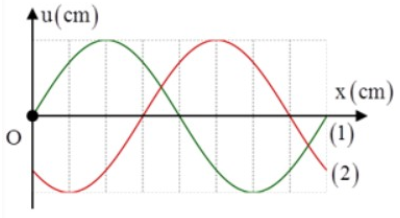
\includegraphics[scale=1]{../figs/VN12-2021-PH-TP015-2}
		\end{center}
		
		Chu kì của sóng là
		\begin{mcq}(4)
			\item $\SI{0.9}{s}$.
			\item $\SI{0.4}{s}$.
			\item $\SI{0.6}{s}$.
			\item $\SI{0.8}{s}$.
		\end{mcq}
	}
	\loigiai{
		\textbf{Đáp án D.}
		
		Từ đồ thị ta thấy trong khoảng thời gian $\Delta t = \SI{0.3}{s}$, đỉnh sóng đi được quãng đường $S=\SI{3}{cm}$.
		
		Vận tốc truyền sóng: $v=\dfrac{S}{\Delta t} = \SI{10}{cm/s}$.
		
		Bước sóng của sóng: $\lambda = \SI{8}{cm}$.
		
		Vậy chu kì của sóng là $T=\dfrac{\lambda}{v} = \SI{0.8}{s}$.
	}
	
	\item \mkstar{3}
	
	\cauhoi{
		Hai điểm A, B nằm trên cùng một đường thẳng đi qua một nguồn âm điểm phát ra âm đẳng hướng và ở hai phía so với nguồn âm. Biết mức cường độ âm tại A và tại trung điểm của AB lần lượt là $\SI{50}{dB}$ và $\SI{44}{dB}$. Mức cường độ âm tại B là
		
		\begin{mcq}(4)
			\item $\SI{28}{dB}$.
			\item $\SI{36}{dB}$.
			\item $\SI{38}{dB}$.
			\item $\SI{47}{dB}$.
		\end{mcq}
	}
	\loigiai{
		\textbf{Đáp án B.}
		
		Vì A, B nằm hai bên nguồn O nên $\text{OM} = \dfrac{\text{OB} - \text{OA}}{2}$.
		
		$$L_\text{A} - L_\text{M} = 20 \log \dfrac{\text{OM}}{\text{OA}} = 6 \Rightarrow \text{OM} = 2 \text{OA} \Rightarrow \text{OB} = 5 \text{OA}.$$
		
		$$L_\text{A} - L_\text{B} = 20 \log \dfrac{\text{OB}}{\text{OA}} = 20 \log 5 \Rightarrow L_\text{B} = 50 - 20 \log 5 = \SI{36}{dB}.$$
	}
	
	\item \mkstar{3}
	
	\cauhoi{
		Hai họa âm liên tiếp do một dây đàn phát ra có tần số hơn kém nhau $\SI{56}{Hz}$. Họa âm thứ ba và họa âm thứ năm có tần số lần lượt bằng bao nhiêu?
		
		\begin{mcq}(2)
			\item $\SI{162}{Hz}$ và $\SI{280}{Hz}$.
			\item $\SI{16}{Hz}$ và $\SI{28}{Hz}$.
			\item $\SI{12}{Hz}$ và $\SI{20}{Hz}$.
			\item $\SI{126}{Hz}$ và $\SI{208}{Hz}$.
		\end{mcq}
	}
	\loigiai{
		\textbf{Đáp án A.}
		
		Hai họa âm liên tiếp hơn kém nhau $\SI{56}{Hz}$ nên ta có:
		$$f_n - f_{n-1} = 56 \Leftrightarrow nf_1 - (n-1)f_1 = 56 \Rightarrow f_1 = \SI{56}{Hz}.$$
		
		Từ đó ta có tần số của họa âm thứ ba và thứ năm là
		$$f_3 = 3f_1 = \SI{162}{Hz}$$
		$$f_5 = 5f_1 = \SI{280}{Hz}$$
	}
	
	\item \mkstar{3}
	
	\cauhoi{
		Một sợi dây đàn hồi căng ngang, đang có sóng dừng ổn định. Khoảng thời gian giữa hai lần liên tiếp sợi dây duỗi thẳng là $\SI{0.1}{s}$. tốc độ truyền sóng trên dây là $\SI{3}{m/s}$. Khoảng cách giữa hai điểm gần nhau nhất trên sợi dây dao động cùng pha và có biên độ dao động bằng một nửa biên độ của bụng sóng là
		
		\begin{mcq}(4)
			\item $\SI{10}{cm}$.
			\item $\SI{8}{cm}$.
			\item $\SI{20}{cm}$.
			\item $\SI{30}{cm}$.
		\end{mcq}
	}
	\loigiai{
		\textbf{Đáp án C.}
		
		Khoảng thời gian giữa hai lần liên tiếp sợi dây duỗi thẳng là $\dfrac{T}{2} = \SI{0.1}{s}$, suy ra $T=\SI{0.2}{s}$. Suy ra bước sóng:
		$$\lambda = v T = \SI{0.6}{m}.$$
		
		Khoảng cách từ một điểm nút đến vị trí có biên độ bằng nửa biên độ cực đại là $\dfrac{\lambda}{2}$.
		
		Hai điểm gần nhau nhất trên sợi dây dao động cùng pha, suy ra 2 điểm đó cùng thuộc một bó sóng.
		
		Khoảng cách cần tìm:
		$$\dfrac{\lambda}{2} - \dfrac{\lambda}{12} - \dfrac{\lambda}{3} = \dfrac{\lambda}{3} = \SI{20}{cm}.$$
	}
	
	\item \mkstar{3}
	
	\cauhoi{
		Tại hai điểm A, B trên mặt chất lỏng cách nhau $\SI{15}{cm}$ có hai nguồn phát sóng kết hợp, dao động theo phương trình $u_1 = a \cos 40\pi t\ \text{cm}$ và $u_2 = b \cos (40\pi t + \pi)\ \text{cm}$. Tốc độ truyền sóng trên bề mặt chất lỏng là $\SI{40}{cm/s}$. Gọi E, F là hai điểm trên đoạn AB sao cho $\text{AE} = \text{EF} = \text{FB}$. Tìm số cực đại trên $\text{EF}$.
		
		\begin{mcq}(4)
			\item 5.
			\item 6.
			\item 4.
			\item 7.
		\end{mcq}
	}
	\loigiai{
		\textbf{Đáp án B.}
		
		Tại E ($d_1=\SI{5}{cm}$; $d_2 = \SI{10}{cm}$) suy ra $\Delta d_\text{E} = \SI{5}{cm}$.
		
		Tại F ($d_1=\SI{10}{cm}$; $d_2=\SI{5}{cm}$) suy ra $\Delta d_\text{F} = \SI{-5}{cm}$.
		
		$$\lambda = \dfrac{v}{f} = \SI{2}{cm}.$$
		
		Vì 2 nguồn dao động ngược pha: $\Delta \varphi = \xsi{\pi}{rad}$.
		
		Số cực đại:
		$$\dfrac{\Delta d_\text{F}}{\lambda} - \dfrac{\Delta \varphi}{2\pi} \leq k \leq \dfrac{\Delta d_\text{E}}{\lambda} - \dfrac{\Delta \varphi}{2\pi} \Rightarrow -3 \leq k \leq 2.$$
		
		Có 6 điểm dao động cực đại.
	}
	
	\item \mkstar{3}
	
	\cauhoi{
		Thực hiện thí nghiệm giao thoa sóng cơ trên mặt chất lỏng với hai nguồn cùng pha có cùng tần số $f=\SI{30}{Hz}$, vận tốc truyền sóng trong môi trường là $\SI{150}{cm/s}$. Trên mặt chất lỏng có 4 điểm có tọa độ lần lượt như sau: M ($d_1=\SI{25}{cm};\ d_2 = \SI{30}{cm}$); N ($d_1=\SI{5}{cm};\ d_2=\SI{10}{cm}$); O ($d_1 = \SI{7}{cm};\ d_2=\SI{12}{cm}$); P ($d_1 = \SI{27.5}{cm};\ d_2=\SI{30}{cm}$). Hỏi có mấy điểm nằm trên đường cực đại số 1?
		
		\begin{mcq}(4)
			\item 1.
			\item 2.
			\item 3.
			\item 4.
		\end{mcq}
	}
	\loigiai{
		\textbf{Đáp án C.}
		
		Ta có $\lambda = \dfrac{v}{f} = \SI{5}{cm}$.
		
		Tại M: $\Delta d= d_2 - d_1 = \SI{5}{cm} = \lambda \Rightarrow$ nằm trên đường cực đại số 1.
		
		Tại N: $\Delta d= d_2 - d_1 = \SI{5}{cm} = \lambda \Rightarrow$ nằm trên đường cực đại số 1.
		
		Tại O: $\Delta d= d_2 - d_1 = \SI{5}{cm} = \lambda \Rightarrow$ nằm trên đường cực đại số 1.
		
		Tại P: $\Delta d= d_2 - d_1 = \SI{2.5}{cm} = \dfrac{\lambda}{2} \Rightarrow$ nằm trên đường cực tiểu số 1.
		
		Có 3 điểm M, N, O nằm trên đường cực đại số 1.
	}
	
	\item \mkstar{3}
	
	\cauhoi{
		Ở mặt nước có hai nguồn kết hợp đặt tại hai điểm A và B, dao động cùng pha theo phương thẳng đứng, phát ra hai sóng có bước sóng $\lambda$. Trên AB có 9 vị trí mà ở đó các phần tử nước dao động với biên độ cực đại. Gọi C và D là hai điểm ở mặt nước sao cho ABCD tạo thành hình vuông. Gọi M là một điểm thuộc cạnh CD và nằm trên vân cực đại giao thoa bậc nhất ($\text{MA} - \text{MB} = \lambda$). Biết phần tử tại M dao động cùng pha với các nguồn. Độ dài đoạn AB \textbf{gần nhất} với giá trị nào sau đây?
		
		\begin{mcq}(4)
			\item $\SI{4.6}{\lambda}$.
			\item $\SI{4.8}{\lambda}$.
			\item $\SI{4.4}{\lambda}$.
			\item $\SI{4.7}{\lambda}$.
		\end{mcq}
	}
	\loigiai{
		\textbf{Đáp án B.}
		
		\begin{center}
			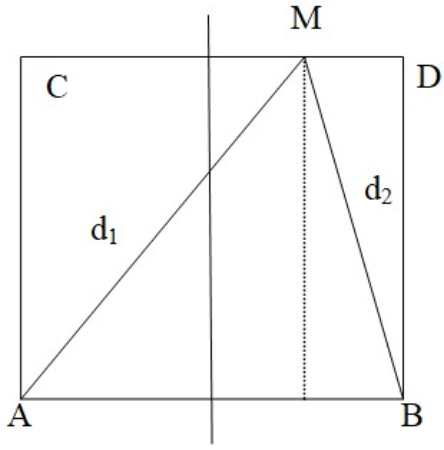
\includegraphics[scale=0.8]{../figs/VN12-2021-PH-TP015-6}
		\end{center}
	
		M là cực đại giao thoa và cùng pha với hai nguồn nên $d_1 - d_2 = n \lambda$, $d_1 + d_2 = m \lambda$, với $n$, $m$ là số nguyên cùng lẻ hoặc cùng chẵn.
		
		Vì $n=1 \Rightarrow m$ là số lẻ.
		
		Ta có: $d_1 + d_2 > \text{AB}$, $4\lambda \leq \text{AB} \leq 5 \lambda$.
		
		Từ các phương trình trên, ta có: $d_1 - d_2 = \lambda$, $d_1 + d_2 = 11 \lambda$.
		
		Suy ra: $d_1 = 6 \lambda$, $d_2 = 5 \lambda$.
		
		Ta có: $\sqrt{(6\lambda)^2 - \text{AB}^2} + \sqrt{(5 \lambda)^2 - \text{AB}^2} = \text{AB}^2 \Rightarrow \text{AB} = \SI{4.8336}{\lambda}$.
	}
	
	\item \mkstar{3}
	
	\cauhoi{
		Hai nguồn sóng kết hợp $\text{S}_1$ và $\text{S}_2$ nằm trên mặt chất lỏng, thực hiện các dao động điều hòa theo phương vuông góc với mặt chất lỏng với hiệu số pha ban đầu bằng $\varphi$. Biết rằng trên đường nối hai nguồn, trong số những điểm có biên độ dao động bằng 0 thì điểm M gần đường trung trực nhất cách đường trung trực một khoảng bằng $\lambda /6$. Hiệu số pha ban đầu $\varphi$ có giá trị bằng
		
		\begin{mcq}(4)
			\item $\dfrac{2\pi}{3}\ \text{rad}$.
			\item $\dfrac{\pi}{2}\ \text{rad}$.
			\item $\dfrac{\pi}{3}\ \text{rad}$.
			\item $\dfrac{\pi}{6}\ \text{rad}$.
		\end{mcq}
	}
	\loigiai{
		\textbf{Đáp án C.}
		
		Điểm cực tiểu (là điểm M) trên $\text{S}_1 \text{S}_2$ nằm gần điểm cực đại trung tâm nhất (là điểm O) cách O một khoảng bằng $\lambda / 4$. Gọi trung điểm của $\text{S}_1 \text{S}_2$ là I.
		
		TH1: điểm M nằm giữa I và O. Ta có $\text{IM} + \text{MO} = \text{IO}$, suy ra:
		$$\dfrac{\lambda}{6} + \dfrac{\lambda}{4} = \dfrac{\Delta \varphi \lambda}{4\pi} \Rightarrow \Delta \varphi = \xsi{\dfrac{5\pi}{3}}{rad}.$$
		
		TH2: điểm I nằm giữa M và O. Ta có $\text{IM} + \text{IO} = \text{MO}$, suy ra:
		$$\dfrac{\lambda}{6} + \dfrac{\Delta \varphi \lambda}{4\pi} = \dfrac{\lambda}{4} \Rightarrow \Delta \varphi = \xsi{\dfrac{\pi}{3}}{rad}.$$
	}
	
	\item \mkstar{3}
	
	\cauhoi{
		Hai nguồn âm nhỏ giống nhau phát ra âm thanh cùng pha, cùng biên độ và cùng tần số tại A và B. Tai của một người ở điểm N với $\text{AN} = \SI{2}{m}$ và $\text{BN} = \SI{1.625}{m}$. Tốc độ truyền âm trong không khí là $\SI{330}{m/s}$. Bước sóng dài nhất để người này không nghe được âm thanh từ hai nguồn phát ra là
		
		\begin{mcq}(4)
			\item $\SI{0.375}{m}$.
			\item $\SI{0.75}{m}$.
			\item $\SI{0.50}{m}$.
			\item $\SI{0.25}{m}$.
		\end{mcq}
	}
	\loigiai{
		\textbf{Đáp án B.}
		
		Để tai người này không nghe được âm thì tai đặt ở vị trí cực tiểu giao thoa:
		$$\text{AN} - \text{BN} = \left(k + \dfrac{1}{2}\right) \lambda \Rightarrow \lambda = \dfrac{\text{AN} - \text{BN}}{k + \SI{0.5}{}}.$$
		
		Bước sóng lớn nhất ứng với $k=0$, khi đó:
		$$\lambda = \dfrac{\text{AN} - \text{BN}}{\SI{0.5}{}} = \SI{0.75}{m}.$$
	}
	
	\item \mkstar{3}
	
	\cauhoi{
		Trong giờ thực hành hiện tượng sóng dừng trên dây, một học sinh thực hiện như sau: tăng dần tần số của máy phát dao động thì thấy rằng khi sóng dừng xuất hiện trên dây tương ứng với 1 bó sóng và 9 bó sóng thì tần số thu được thỏa mãn $f_9 - f_1 = \SI{200}{Hz}$. Khi trên dây xuất hiện sóng dừng với 6 nút sóng thì máy phát tần số ở giá trị là
		
		\begin{mcq}(4)
			\item $\SI{150}{Hz}$.
			\item $\SI{125}{Hz}$.
			\item $\SI{100}{Hz}$.
			\item $\SI{120}{Hz}$.
		\end{mcq}
	}
	\loigiai{
		\textbf{Đáp án B.}
		
		Với sóng dừng trên dây có hai đầu cố định thì chiều dài sợi dây phải thỏa:
		$$l=k \dfrac{v}{2f} \Rightarrow f =\dfrac{kv}{2l}.$$
		
		Với $f_9 - f_1 = \SI{200}{Hz}$, ta được:
		$$\dfrac{9v}{2l} - \dfrac{v}{2l} = \dfrac{8v}{2l} = \SI{200}{Hz} \Rightarrow \dfrac{v}{2l} = \dfrac{200}{8}.$$
		
		Với 6 nút sóng thì có 5 bó sóng, thay $k=5$ ta được $f_5$ là
		$$f_5 = \dfrac{5v}{2l} = \SI{125}{Hz}.$$
	}
	
	\item \mkstar{4}
	
	\cauhoi{
		Sóng ngang có tần số $f$ truyền trên một sợi dây đàn hồi rất dài với tốc độ $\SI{4.5}{m/s}$. Xét hai điểm M và N trên cùng một phương truyền sóng, cách nhau một khoảng $x$ nhỏ hơn bước sóng. Sóng truyền từ N đến M. Đồ thị biểu diễn li độ sóng của M và N theo thời gian như hình dưới.
		\begin{center}
			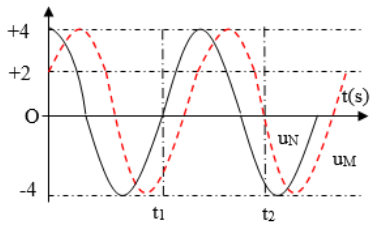
\includegraphics[scale=1]{../figs/VN12-2021-PH-TP015-3}
		\end{center}
		
		Biết $t_1 = \SI{0.05}{s}$. Tại thời điểm $t_2$, khoảng cách giữa phần tử chất lỏng tại M và N có giá trị \textbf{gần nhất} với giá trị nào sau đây?
		\begin{mcq}(4)
			\item $\SI{4.8}{cm}$.
			\item $\SI{6.2}{cm}$.
			\item $\SI{5.7}{cm}$.
			\item $\SI{3.5}{cm}$.
		\end{mcq}
	}
	\loigiai{
		\textbf{Đáp án B.}
		
		Từ đồ thị ta thấy đường N (màu đen) sớm pha hơn M (màu đỏ) một góc là $\Delta \varphi = \xsi{\dfrac{\pi}{3}}{rad}$.
		
		Do đó khoảng cách MN theo phương truyền sóng là $\text{MN} = \dfrac{\lambda}{6}$.
		
		Dựa vào đường màu đen, ta xác định được khoảng thời gian từ $t=0$ đến $t=t_1 = \SI{0.05}{s}$ là $\dfrac{T}{4} + \dfrac{T}{2} = \dfrac{3T}{4}$. Suy ra $T=\xsi{\dfrac{1}{15}}{s}$.
		
		Tính được $\lambda = vT = \SI{30}{cm}$ và $\text{MN} = \SI{5}{cm}$.
		
		Viết phương trình dao động của M và N, ta được:
		$$u_\text{M}=4 \cos \left(30\pi t - \dfrac{\pi}{3}\right)\ \text{cm}.$$
		$$u_\text{N} = 4 \cos (30\pi t)\ \text{cm}.$$
		
		Dựa vào đồ thị thì ta thấy $t_2 = t_1 + \dfrac{T}{2} + \dfrac{T}{6} $, ta xác định được:
		$$|u_\text{M} - u_\text{N}|_{t_2} = \xsi{2\sqrt{3}}{cm}.$$
		$$\Rightarrow \text{MN}_{t_2} = \sqrt{5^2 + 2^2 \cdot 3} = \SI{6.083}{cm}.$$
		
		Vậy $\SI{6.2}{cm}$ là đáp án gần đúng nhất.
	}
	
	\item \mkstar{4}
	
	\cauhoi{
		Một sợi dây đàn hồi căng ngang, đang có sóng dừng ổn định. Trên dây, A là điểm nút, còn B là điểm bụng ở gần A nhất, còn C là trung điểm của AB. Cho $\text{AB} = \SI{10}{cm}$. Biết khoảng thời gian ngắn nhất giữa hai lần mà li độ dao động của phần tử tại B bằng biên độ dao động của phần tử tại C là $\SI{0.2}{s}$. Tốc độ truyền sóng trên dây là
		
		\begin{mcq}(4)
			\item $\SI{2}{m/s}$.
			\item $\SI{0.5}{m/s}$.
			\item $\SI{1}{m/s}$.
			\item $\SI{0.25}{m/s}$.
		\end{mcq}
	}
	\loigiai{
		\textbf{Đáp án B.}
		
		Vì B là điểm bụng gần nút A nhất nên:
		$$\text{AB} = \SI{10}{cm} = \dfrac{\lambda}{4} \Rightarrow \lambda = \SI{40}{cm}.$$
		
		Tại C thì $x=\dfrac{\lambda}{8} = \SI{5}{cm}$. Biên độ dao động của C là
		$$A_\text{C} = 2A \sin \left(\dfrac{2\pi \lambda}{8\lambda}\right) = A\sqrt{2}.$$
		
		Tương tự, biên độ dao động tại B là $2A$.
		
		\begin{center}
			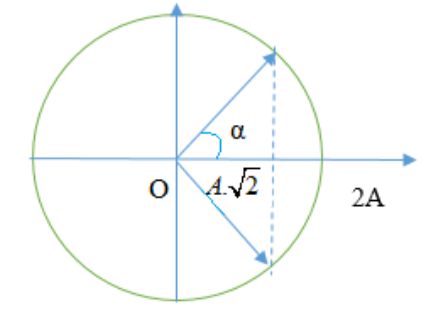
\includegraphics[scale=1]{../figs/VN12-2021-PH-TP015-7}
		\end{center}
	
		Dựa đồ giản đồ vectơ quay, ta có độ lớn góc $\alpha$ là
		$$\alpha = \arccos \dfrac{A \sqrt{2}}{2A} = 45^\circ.$$
		
		Vậy thời gian giữa hai lần liên tiếp B có li độ bằng biên độ của C là
		$$t = \dfrac{2 \cdot 45^\circ}{360^\circ} \cdot T = \dfrac{T}{4}.$$
		
		Vậy chu kì dao động là $T=4t=\SI{0.8}{s}$, vận tốc truyền sóng là $v=\dfrac{\lambda}{T} = \SI{50}{cm}$.
	}
	
	\item \mkstar{4}
	
	\cauhoi{
		Trên một sợi dây dài đang có sóng ngang truyền qua, hình dạng của một đoạn dây tại hai thời điểm $t_1$ và $t_2$ được cho như hình dưới.
		\begin{center}
			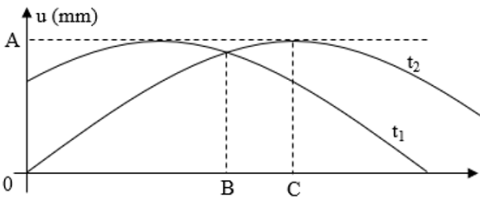
\includegraphics[scale=1]{../figs/VN12-2021-PH-TP015-4}
		\end{center}
	
		Li độ của các phần tử tại B và C ở thời điểm $t_1$ lần lượt là $\xsi{10\sqrt{3}}{mm}$ và $\SI{10}{mm}$. Biết $\Delta t = t_2 - t_1 = \xsi{\dfrac{\SI{0.05}{}}{6}}{s}$ và nhỏ hơn một chu kì sóng. Tốc độ dao động cực đại của các phần tử trên dây bằng
		\begin{mcq}(4)
			\item $\xsi{0,4\pi \sqrt{2}}{m/s}$.
			\item $\xsi{0,4\pi}{m/s}$.
			\item $\xsi{0,8\pi}{m/s}$.
			\item $\xsi{0,8\pi \sqrt{3}}{m/s}$.
		\end{mcq}
	}
	\loigiai{
		\textbf{Đáp án C.}
		
		Từ đồ thị, xác định được các điểm B, C tại thời điểm $t_1$, $t_2$ trên vòng tròn lượng giác:
		\begin{center}
			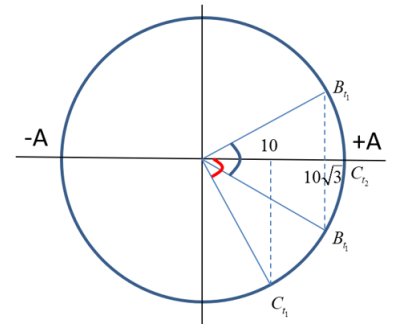
\includegraphics[scale=1]{../figs/VN12-2021-PH-TP015-8}
		\end{center}
	
	Ta có:
	$$\Delta \varphi_{\text C(t_1 \rightarrow t_2)} = \Delta \varphi_{\text B (t_1 \rightarrow t_2)} = \alpha = \omega \Delta t.$$
	
	Từ vòng tròn lượng giác, ta có $\cos \alpha = \dfrac{10}{A}$ và $\cos \dfrac{\alpha}{2} = \dfrac{10\sqrt{3}}{A}$.
	
	Suy ra $\cos \alpha = \dfrac{1}{2} \Rightarrow \alpha = 60^\circ \Rightarrow A = \SI{20}{mm}$.
	
	Mà $\alpha = \omega\Delta t \Rightarrow \omega = \dfrac{\alpha}{\Delta t} = \xsi{40\pi}{rad/s}$.
	
	Tốc độ cực đại:
	$$v_\text{max} = \omega A = \xsi{0,8\pi}{m/s}.$$
	}
	
	\item \mkstar{4}
	
	\cauhoi{
		Một sợi dây đang có sóng dừng ổn định. Sóng truyền trên dây có tần số $\SI{10}{Hz}$ và bước sóng $\SI{6}{cm}$. Trên dây, hai phần tử M và N có vị trí cân bằng cách nhau $\SI{8}{cm}$, M thuộc một bụng sóng dao động điều hòa với biên độ $\SI{6}{mm}$. Lấy $\pi^2 = 10$. Tại thời điểm $t$, phần tử M đang chuyển động với tốc độ $\xsi{6\pi}{cm/s}$ thì phần tử N chuyển động với gia tốc có độ lớn là
		
		\begin{mcq}(4)
			\item $\xsi{6\sqrt{3}}{m/s^2}$.
			\item $\SI{6}{m/s^2}$.
			\item $\xsi{6\sqrt{2}}{m/s^2}$.
			\item $\SI{3}{m/s^2}$.
		\end{mcq}
	}
	\loigiai{
		\textbf{Đáp án A.}
		
		Tần số góc của dao động là
		$$\omega = 2\pi f = 2\pi \cdot \SI{10}{Hz} = \xsi{20\pi}{rad/s}.$$
		
		Biên độ dao động của N là
		$$A_\text{N} = A_\text b \left|\cos \left(\dfrac{2\pi d}{\lambda}\right)\right| = \SI{0.006}{m} \cdot \left|\cos \left(\dfrac{2\pi \cdot \SI{0.08}{m}}{\SI{0.06}{m}}\right)\right| = \SI{0.003}{m}.$$
		
		Tại thời điểm M chuyển động với tốc độ $\xsi{6\pi}{cm/s}$ thì nó có li độ là
		$$\left(\dfrac{x_\text{M}}{A_\text{M}}\right)^2 + \left(\dfrac{v_\text{M}}{v_\text{M max}}\right)^2 = 1 \Rightarrow \left(\dfrac{x}{\SI{0.006}{m}}\right)^2 + \left(\dfrac{6\pi \cdot 10^{-2}\ \text{m/s}}{20\pi\ \text{rad/s} \cdot \SI{0.006}{m}}\right)^2 = 1 \Rightarrow x_\text{M} = \xsi{\dfrac{3\sqrt{3}}{1000}}{m}.$$
		
		Gia tốc của điểm N có thể suy ra bằng cách lập tỉ số giữa gia tốc của M và gia tốc của N:
		$$\left|\dfrac{a_\text{N}}{a_\text{M}}\right| = \left|\dfrac{a_\text{N}}{\omega^2 x_\text{M}}\right| = \dfrac{A_\text{N}}{A_\text{M}} \Rightarrow \left|\dfrac{a_\text{N}}{(20\pi\ \text{rad/s})^2 \cdot \xsi{\dfrac{3\sqrt{3}}{1000}}{m}}\right| = \dfrac{\SI{0.003}{m}}{\SI{0.006}{m}} \Rightarrow |a_\text{N}| = \xsi{6\sqrt{3}}{m/s^2}.$$
	}
	
	\item \mkstar{4}
	
	\cauhoi{
		Tại hai điểm A, B trên mặt nước cách nhau $\SI{16}{cm}$ có hai nguồn phát sóng giống nhau. Điểm M nằm trên mặt nước và trên đường trung trực của AB, cách trung điểm I của AB một khoảng nhỏ nhất bằng $\xsi{5\sqrt{5}}{cm}$ và luôn dao động cùng pha với I. Hỏi điểm N nằm trên mặt nước và nằm trên đường thẳng vuông góc với AB tại A, cách A một khoảng nhỏ nhất bằng bao nhiêu để N dao động với biên độ cực tiểu?
		\begin{mcq}(4)
			\item $\SI{9.22}{cm}$.
			\item $\SI{8.75}{cm}$.
			\item $\SI{2.14}{cm}$.
			\item $\SI{8.57}{cm}$.
		\end{mcq}
	}
	\loigiai{
		\textbf{Đáp án C.}
		
		\begin{center}
			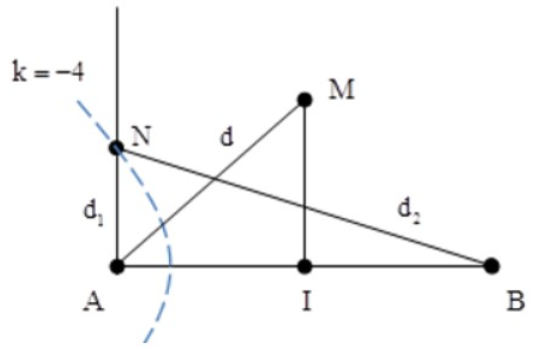
\includegraphics[scale=0.8]{../figs/VN12-2021-PH-TP015-9}
		\end{center}
	
		Vì hai nguồn đồng pha, M, I đều thuộc trung trực của AB nên để M và I dao động cùng pha thì:
		$$\text{MA} - \text{IA} = k \lambda.$$
		
		Mà M gần I nhất nên chọn $k=1$, do đó:
		$$\text{MA} = d_\text{A} = \SI{0.5}{}\text{AB} + \lambda = 8 + \lambda.$$
		
		Mặt khác $\text{MI} = \xsi{4\sqrt{5}}{cm}$ nên
		$$\text{MA} = \xsi{4\sqrt{5}}{cm} \Rightarrow \text{MA} = 8 + \lambda = \sqrt{\left(\dfrac{\text{AB}}{2}\right)^2 + \text{IM}^2} = 12 \Rightarrow \lambda = \SI{4}{cm}.$$
		
		Số điểm dao động với biên độ cực tiểu trên AB:
		$$-\dfrac{\text{AB}}{2} - \dfrac{1}{2} < k < \dfrac{\text{AB}}{2} - \dfrac{1}{2} \Rightarrow \SI{-4.5}{} < k < \SI{3.5}{}.$$
		
		Để N là một điểm cực tiểu và gần A nhất thì N phải nằm trên hyperbol cực tiểu có $k=\SI{-4}{}$. Vậy:
		$$
		\begin{cases}
			d_\text{1N} - d_\text{2N} = \SI{-3.5}{\lambda}\\
			d_\text{2N}^2 = d_\text{1N}^2 + \text{AB}^2
		\end{cases}
	\Rightarrow d_\text{1N} = \SI{2.14}{cm}.
		$$
	}
\end{enumerate}
\loigiai{\textbf{Đáp án}
	\begin{center}
		\begin{tabular}{|m{2.8em}|m{2.8em}|m{2.8em}|m{2.8em}|m{2.8em}|m{2.8em}|m{2.8em}|m{2.8em}|m{2.8em}|m{2.8em}|}
			\hline
			1. B & 2. B & 3. D & 4. A & 5. A & 6. B & 7. C & 8. A & 9. C & 10. D \\
			\hline
			11. B & 12. A & 13. D & 14. C & 15. D & 16. B & 17. A & 18. A & 19. A & 20. D\\
			\hline
			21. A & 22. B & 23. C & 24. C & 25. C & 26. D & 27. B & 28. A & 29. C & 30. B\\
			\hline
			31. C & 32. B & 33. C & 34. B & 35. B & 36. B & 37. B & 38. C & 39. A & 40. C\\
			\hline
		\end{tabular}
\end{center}}
\setcounter{mychapter}{11}
\mychapter{Đại cương về dòng điện xoay chiều}
\startcontents[mychapters]
\printcontents[mychapters]{}{0}{\setcounter{tocdepth}{1}}
\begin{enumerate}[label=\bfseries Câu \arabic*:]
	
	\item \mkstar{1}
	
	\cauhoi{Dòng điện xoay chiều hình sin là dòng điện
		\begin{mcq}
			\item có cường độ không đổi theo thời gian.
			\item có cường độ biến đổi điều hoà theo thời gian.
			\item có chiều không đổi theo thời gian.
			\item có chu kỳ thay đổi theo thời gian.
		\end{mcq}
	}
		\loigiai{
\textbf{Đáp án: B.}
			
			Dòng điện xoay chiều là dòng điện có cường độ biến đổi điều hoà theo thời gian.
			
			}	
	
	%%%%%%%%%%%%%%CÂU2%%%%%%%%%%
	\item \mkstar{1}
	
	\cauhoi{Trong các đại lượng đặc trưng cho dòng điện xoay chiều sau đây, đại lượng nào có dùng giá trị hiệu dụng?
		\begin{mcq}(4)
			\item Điện áp. 
			\item Chu kỳ.
			\item Tần số. 
			\item Công suất.
		\end{mcq}
}	
		\loigiai{
			\textbf{Đáp án: A.}
			
			Trong các đại lượng đặc trưng cho dòng điện xoay chiều, đại lượng có dùng giá trị hiệu dụng là điện áp, cường độ dòng điện, suất điện động.
			
			}	
	
	%%%%%%%%%%%%%%CÂU3%%%%%%%%%%
	\item \mkstar{1}
	
	\cauhoi{Trong các đại lượng đặc trưng cho dòng điện xoay chiều sau đây, đại lượng nào \textbf{không} dùng giá trị hiệu dụng?
		\begin{mcq}(2)
			\item Điện áp.   
			\item Cường độ dòng điện.
			\item Suất điện động.   
			\item Công suất.
		\end{mcq}
}	
		\loigiai{
			\textbf{Đáp án: D.}
			
			Công suất không có giá trị hiệu dụng.
			
			}	
	%%%%%%%%%%%%%%CÂU4%%%%%%%%%%
	\item \mkstar{1}
	
	\cauhoi{Phát biểu nào sau đây là\textbf{ không} đúng?
		\begin{mcq}
			\item Điện áp biến đổi điều hoà theo thời gian gọi là điện áp xoay chiều.
			\item Dòng điện có cường độ biến đổi điều hoà theo thời gian gọi là dòng điện xoay chiều.
			\item Suất điện động biến đổi điều hoà theo thời gian gọi là suất điện động xoay chiều.
			\item Cho dòng điện một chiều và dòng điện xoay chiều lần lượt đi qua cùng một điện trở thì chúng toả ra nhiệt lượng như nhau.
		\end{mcq}
}	
		\loigiai{
			\textbf{Đáp án: D.}
			
			Cho dòng điện một chiều và dòng điện xoay chiều lần lượt đi qua cùng một điện trở thì chúng toả ra nhiệt lượng như nhau là không đúng vì chưa đề cập đến độ lớn của cường độ dòng điện. Nếu muốn chúng tỏa ra cùng một nhiệt lượng thì cường độ dòng điện một chiều phải có giá trị bằng giá trị hiệu dụng của dòng điện xoay chiều.
			
			}	
	
	%%%%%%%%%%%%%%CÂU5%%%%%%%%%%
	\item \mkstar{1}
	
	\cauhoi{Các giá trị hiệu dụng của dòng điện xoay chiều
		\begin{mcq}
			\item được xây dựng dựa trên tác dụng nhiệt của dòng điện.
			\item chỉ được đo bằng ampe kế nhiệt.
			\item bằng giá trị trung bình chia cho $\sqrt{2}$.
			\item bằng giá trị cực đại chia cho 2.
		\end{mcq}
}		
		\loigiai{
		\textbf{Đáp án: A.}
			
			Các giá trị hiệu dụng của dòng điện xoay chiều được xây dựng dựa trên tác dụng nhiệt của dòng điện.
			
			}	
	
	%%%%%%%%%%%%%%CÂU6%%%%%%%%%%
	\item \mkstar{1}
	
	
	\cauhoi{Cường độ dòng điện trong mạch không phân nhánh có dạng $i=2\sqrt{2}\cos(100\pi t)\,\text{A}$. Cường độ dòng điện hiệu dụng trong mạch là
		\begin{mcq}(4)
			\item $I=\SI{4}{A}$.
			\item $I=\SI{2,83}{A}$.
			\item $I=\SI{2}{A}$.
			\item $I=\SI{1,41}{A}$.
		\end{mcq}
}	
		\loigiai{
		\textbf{Đáp án: C.}
			
			Cường độ dòng điện hiệu dụng $$I=\dfrac{I_0}{\sqrt{2}}=\SI{2}{A}.$$
			
			}
	
	
	
	%%%%%%%%%%%%%%CÂU7%%%%%%%%%%
	\item \mkstar{1}
	
	
	\cauhoi{Điện áp tức thời giữa hai đầu đoạn mạch có dạng $i=141\cos(100\pi t)\,\text{V}$. Điện áp hiệu dụng giữa hai đầu đoạn mạch là
		\begin{mcq}(4)
			\item $\SI{141}{V}$.
			\item $\SI{50}{V}$.
			\item $\SI{100}{V}$.
			\item $\SI{200}{V}$.
		\end{mcq}
}		
		\loigiai{
				\textbf{Đáp án: C.}
			
			Điện áp hiệu dụng $$U=\dfrac{U_0}{\sqrt{2}}=\SI{100}{V}.$$
			
		}	
	\item \mkstar{2}

\cauhoi{Phát biểu nào sau đây là \textbf{không} đúng?
	\begin{mcq}
		\item Dòng điện xoay chiều không phải là dòng điện chạy trong các đồ chơi dùng pin.
		\item Dòng điện dân dụng ở Việt Nam là dòng điện xoay chiều.
		\item Dòng điện xoay chiều là dòng điện hình sin.
		\item Dòng điện hình sin là dòng điện xoay chiều.
	\end{mcq}
}	
\loigiai{
	\textbf{Đáp án: C.}
	
	Dòng điện hình sin là dòng điện xoay chiều.
	
	Nhưng dòng điện xoay chiều có thể không phải là dòng điện hình sin mà còn là các hình dạng khác.
	
}		
	\item \mkstar{2}

\cauhoi{Đơn vị nào sau đây dùng để tính lượng điện năng tiêu thụ hàng tháng của một hộ gia đình?
	\begin{mcq}(2)
		\item Am-pe.
		\item Oát.
		\item Ki-lô Oát trên giờ.
		\item Ki-lô Oát giờ.
	\end{mcq}
}	
\loigiai{
	\textbf{Đáp án: D.}
	
	Đơn vị để tính điện năng tiêu thụ là kWh. Với $1\ \text{kWh} = \SI{3e6}{\joule}$.
	
}			
	
	%%%%%%%%%%%%%%CÂU8%%%%%%%%%%
	\item \mkstar{2}
	
	\cauhoi{ Một điện trở thuần $R=\SI{100}{\Omega}$ khi dùng dòng điện có tần số $\SI{50}{Hz}$. Nếu dùng dòng điện có tần số $\SI{100}{Hz}$ thì điện trở
		\begin{mcq}(4)
			\item giảm 2 lần.
			\item tăng 2 lần.
			\item không đổi.
			\item giảm 4 lần.
		\end{mcq}
}	
		\loigiai{
		\textbf{Đáp án: C.}
			
			Giá trị của điện trở không phụ thuộc vào tần số của mạch.
			
			}	
	
	%%%%%%%%%%%%%%CÂU9%%%%%%%%%%
		\item \mkstar{2}
	
	\cauhoi{Dòng điện có biểu thức $i=2\cos100\pi t\, \text{A}$, trong một chu kì, dòng điện đổi chiều bao nhiêu lần?
		\begin{mcq}(4)
			\item 100 lần.
			\item 50 lần.
			\item 2 lần.
			\item 1 lần.
		\end{mcq}
	}	
	\loigiai{
		\textbf{Đáp án: C.}
		
		Trong 1 chu kì, dòng điện đổi chiều 2 lần.
		
	}
		\item \mkstar{2}

\cauhoi{Dòng điện có biểu thức $i=2\cos100\pi t\, \text{A}$, trong $1/50\ \text s$, dòng điện đổi chiều bao nhiêu lần?
	\begin{mcq}(4)
		\item 100 lần.
		\item 50 lần.
		\item 2 lần.
		\item 1 lần.
	\end{mcq}
}	
\loigiai{
	\textbf{Đáp án: C.}
	
 $1/50\ \text s$ tương ứng với 1 chu kì. Vậy dòng điện đổi chiều 2 lần.
	
}		
		\item \mkstar{2}
	
	\cauhoi{Dòng điện có biểu thức $i=2\cos100\pi t\, \text{A}$, trong một giây, dòng điện đổi chiều bao nhiêu lần?
		\begin{mcq}(4)
			\item 100 lần.
			\item 50 lần.
			\item 110 lần.
			\item 99 lần.
		\end{mcq}
	}	
	\loigiai{
		\textbf{Đáp án: A.}
		
		1 giây tương ứng với 50 chu kì.
		
		Vậy số lần đổi chiều của dòng điện trong một giây là $n=\text{100 lần}$.
		
	}
		\item \mkstar{2}

\cauhoi{Một khung dây dẫn có diện tích $S=\SI{50}{\centi \meter \squared}$ gồm 150 vòng dây quay đều với vận tốc $n\ \text{vòng/ phút}$ trong một từ trường đều $\vec B$ vuông góc với trục quay $\Delta$ và có độ lớn $B=\SI{0.02}{\tesla}$. Từ thông cực đại gửi qua khung là
	\begin{mcq}(4)
		\item $\SI{0.015}{\weber}$.
		\item $\SI{0.15}{\weber}$.
		\item $\SI{1.5}{\weber}$.
		\item $\SI{15}{\weber}$.
	\end{mcq}
}	
\loigiai{
	\textbf{Đáp án: A.}
	
	Đổi $\SI{50}{\centi \meter \squared} = \SI{50e-4}{\meter \squared}$.
	
	Từ thông cực đại gửi qua khung là
	$$\Phi_0=NBS = \SI{0.015}{\weber}.$$
	
}		
		\item \mkstar{2}

\cauhoi{Một khung dây dẫn có diện tích $S=\SI{50}{\centi \meter \squared}$ gồm 150 vòng dây quay đều với vận tốc $n\ \text{vòng/ phút}$ trong một từ trường đều $\vec B$ song song với trục quay $\Delta$ và có độ lớn $B=\SI{0.02}{\tesla}$. Từ thông cực đại gửi qua khung là
	\begin{mcq}(4)
		\item $\SI{0.015}{\weber}$.
		\item $\SI{0}{\weber}$.
		\item $\SI{0.05}{\weber}$.
		\item $\SI{0.15}{\weber}$.
	\end{mcq}
}	
\loigiai{
	\textbf{Đáp án: B.}
	
	Vì $\vec B$ song song với trục quay $\Delta$ nên $\cos \alpha=0$.
	
	Từ thông cực đại gửi qua khung là
	$$\Phi_0=NBS\cos\alpha = \SI{0}{\weber}.$$
	
}	
		\item \mkstar{2}

\cauhoi{Một khung dây hình chữ nhật quay đều với tốc độ góc $3000\ \text{vòng/ phút}$ quanh trục $\Delta$ đặt trong từ trường đều có cảm ứng từ vuông góc với trục quay. Suất điện động trong khung biến thiên điều hòa với chu kì
	\begin{mcq}(4)
		\item $\SI{3.14}{\second}$.
		\item $\SI{0.314}{\second}$.
		\item $\SI{0.02}{\second}$.
		\item $\SI{0.2}{\second}$.
	\end{mcq}
}	
\loigiai{
	\textbf{Đáp án: C.}
	
	Đổi $\omega = 30000\ \text{vòng / phút} \rightarrow\ \omega= \xsi{100\pi}{\radian/ \second}$.
	
	Suất điện động trong khung biến thiên với chu kì là
	$$T = \dfrac{2\pi}{\omega} = \SI{0.02}{\second}.$$
	
}	
\item \mkstar{3}

\cauhoi{Một khung dây dẫn quay đều quanh trục $\Delta$ với tốc độ $150\ \text{vòng/ phút}$ trong từ trường đều có cảm ứng từ $\vec{B}$ vuông góc với trục quay của khung. Từ thông cực đại gửi qua khung dây là $10/ \pi \ \text{Wb}$. Suất điện động hiệu dụng trong khung dây bằng
	\begin{mcq}(4)
		\item $25\ \text V$.
		\item $25\sqrt 2 \text V$.
		\item $50\ \text V$.
		\item $50\sqrt 2 \ \text V$.
	\end{mcq}
}	
\loigiai{\textbf{Đáp án: B.}
	
	Đổi $\omega = 150\ \text{vòng / phút} \rightarrow\ \omega= \xsi{5\pi}{\radian/ \second}$.
	
	Biểu thức liên hệ giữa từ thông cực đại và suất điện động cực đại:
	$$\calE_0 = \omega \Phi_0.$$
	
	
	Suất điện động hiệu dụng trong khung là
	$$\calE=\dfrac{\calE_0}{\sqrt 2} = \dfrac{\omega \Phi_0}{\sqrt 2} = 25\sqrt 2\ \text V.$$
	
	}
	%%%%%%%%%%%%%%CÂU10%%%%%%%%%%
	\item \mkstar{3}
	
	\cauhoi{Một mạch điện xoay chiều có phương trình dòng điện trong mạch là $i=5\cos\left(100\pi t-\dfrac{\pi}{2}\right)\, \text{A}$. Xác định điện lượng chuyển qua mạch trong 1/6 chu kì đầu tiên.
		\begin{mcq}(4)
			\item $\dfrac{1}{40\pi}\,\text{C}$.
			\item $\dfrac{1}{40}\,\text{C}$.
			\item $\dfrac{1}{20\pi}\,\text{C}$.
			\item $\dfrac{1}{20}\,\text{C}$.
		\end{mcq}
}	
		\loigiai{
			\textbf{Đáp án: A.}
			
			Điện lượng chuyển qua mạch trong 1/6 chu kì đầu tiên là
			$$q=\int_{0}^{\frac{T}{6}}{idt}= \int_{0}^{\frac{T}{6}}{5\cos\left(100\pi t-\dfrac{\pi}{2}\right)dt}=\dfrac{1}{40\pi}\,\text{C}.$$
			
			}
		
\item \mkstar{3}

\cauhoi{Một bóng đèn có ghi 110 V - 200 W mắc nối tiếp với điện trở $R$ vào một mạch xoay chiều có $u = 220\sqrt 2 \cos 100 \pi t$ (V). Để đèn sáng bình thường, $R$ phải có giá trị là bao nhiêu?
	\begin{mcq}(4)
		\item $R=\text{60,5}\, \Omega.$
		\item $R=\text{40,5}\, \Omega.$
		\item $R=\text{35,5}\, \Omega.$
		\item $R=\text{30,5}\, \Omega.$
	\end{mcq}
}	
	\loigiai{
	\textbf{Đáp án: A.}
		
		Điện áp hiệu dụng giữa hai đầu đoạn mạch đó là: 
		$$U=\dfrac{U_0}{\sqrt{2}}=\dfrac{220 \sqrt 2\,\si{\volt}}{\sqrt 2}=220 \, \si{\volt}.$$
		
		Bóng đèn và điện trở R mắc nối tiếp nên: $$U = U_\textrm{Đ} + U_R \Rightarrow U_R = \SI{110}{\volt}.$$
		
		Cường độ dòng  điện qua điện trở: $$I=I_R=I_\textrm{Đ}=\dfrac{\calP_\textrm{Đ}}{U_\textrm{Đ}}=\dfrac{20}{11}\, \text{A}.$$
		
		Để đèn sáng bình thường: $$R=\dfrac{U_R}{I_R}=\text{60,5}\, \Omega.$$
		
	}
	\item \mkstar{3}
	
	\cauhoi{Một đèn điện có ghi $110\ \text V - 100\ \text W$ mắc nối tiếp với điện trở $R$ vào một mạch điện xoay chiều có $u=220 \sqrt 2 \sin 100 \omega t\ \text{(V)}$. Để đèn sáng bình thường, $R$ phải có giá trị là bao nhiêu?
		\begin{mcq}(4)
			\item $\SI{1210}{\Omega}$.
			\item $\xsi{10/11}{\Omega}$.
			\item $\SI{121}{\Omega}$.
			\item $\SI{110}{\Omega}$.
		\end{mcq}
	}	
	\loigiai{
		\textbf{Đáp án: C.}
		
		Điện áp định mức của đèn là $U=110\ \text V$.
		
		Công suất định mức của đèn là $\calP = 100\ \text W$.
		
		Điện trở của đèn là
		$$R_\text{đ}=\dfrac{U_\text{đm}^2}{\calP_\text{đm}} = 121\ \Omega.$$
		
		
		Cường độ dòng điện hiệu dụng chạy qua mạch:
		$$I=\dfrac{U}{R_\text{đ} + R} = \dfrac{220}{121+R}.$$
		
		
		Do mạch mắc nối tiếp nên cường độ dòng điện hiệu dụng chạy qua đèn cũng bằng $I$, suy ra điện áp giữa hai đầu bóng đèn là
		$$U_\text{đ} = IR_\text{đ} = \dfrac{220\cdot121}{121+R}.$$
		
		
		Để đèn sáng bình thường thì $U_\text{đ}=U_\text{đm}$, suy ra
		$$	\dfrac{220\cdot121}{121+R} = 110 \Rightarrow R = 121\ \Omega.$$
		
	}
\end{enumerate}
\loigiai{\textbf{Đáp án}
	\begin{center}
		\begin{tabular}{|m{2.8em}|m{2.8em}|m{2.8em}|m{2.8em}|m{2.8em}|m{2.8em}|m{2.8em}|m{2.8em}|m{2.8em}|m{2.8em}|}
			\hline
			1. B & 2. A & 3. D & 4. D & 5. A & 6. C  & 7. C  & 8. C & 9. D & 10. C\\
			\hline
			11. C & 12. C & 13. A & 14. A & 15. B & 16. C  & 17. B  & 18. A & 19. A & 20. C\\
			\hline
		\end{tabular}
\end{center}}
\stopcontents[mychapters]
\setcounter{mychapter}{12}
\mychapter{Các mạch điện xoay chiều}
\startcontents[mychapters]
\printcontents[mychapters]{}{0}{\setcounter{tocdepth}{1}}
\begin{enumerate}[label=\bfseries Câu \arabic*:]
	
	\item \mkstar{1}
	
\cauhoi{Một mạch điện xoay chiều chỉ có cuộn thuần cảm, mối quan hệ về pha của $u$ và $i$ trong mạch là
		\begin{mcq}(2)
			\item $u$ và $i$ cùng pha với nhau.
			\item $u$ sớm pha hơn $i$ góc $\pi/2$.
			\item $u$ và $i$ ngược pha với nhau.
			\item $i$ sớm pha hơn $u$ góc $\pi/2$.
		\end{mcq}
}		
		\loigiai{
		\textbf{Đáp án: B.}
			
			Một mạch điện xoay chiều chỉ có cuộn thuần cảm, mối quan hệ về pha của $u$ và $i$ trong mạch là $u$ sớm pha hơn $i$ góc $\pi/2$.
			
			}
	
	%%%%%%%%%%%%%%CÂU2%%%%%%%%%%
	\item \mkstar{2}
	
	\cauhoi{Mạch điện $X$ chỉ có một phần tử có phương trình dòng điện và hiệu điện thế lần lượt như sau $i=2\sqrt{2}\cos\left(100\pi t+\dfrac{\pi}{6}\right)\,\text{A}$ và $u=200\sqrt{2}\cos\left(100\pi t+\dfrac{\pi}{6}\right)\,\text{V}$. Hãy xác định đó là phần tử gì và độ lớn bao nhiêu?
		\begin{mcq}(4)
			\item $Z_L=\SI{100}{\ohm}$.
			\item $Z_C=\SI{100}{\ohm}$.
			\item $R=\SI{100}{\ohm}$.
			\item $R=100\sqrt{2}\SI{}{\ohm}$.
		\end{mcq}
}		
		\loigiai{
			\textbf{Đáp án: C.}
			
			Vì $u$ và $i$ cùng pha nên đây là $R$, $R=\dfrac{U_0}{I_0}=\SI{100}{\ohm}.$
			
		}
	
	
	%%%%%%%%%%%%%%CÂU3%%%%%%%%%%
	\item \mkstar{2}
	
	\cauhoi{Một mạch điện chỉ có cuộn cảm có hệ số tự cảm $L=\dfrac{1}{\pi}\,\text{H}$ mắc vào mạng điện và có phương trình dòng điện $i=2\cos\left(100\pi t+\dfrac{\pi}{6}\right)\,\text{A}$. Hãy viết phương trình hiệu điện thế giữa hai đầu mạch điện.
		\begin{mcq}(2)
			\item $u_L=200\cos\left(100\pi t+\dfrac{2\pi}{3}\right)\,\text{V}$.
			\item $u_L=200\cos\left(100\pi t+\dfrac{\pi}{6}\right)\,\text{V}$.
			\item $u_L=200\sqrt{2}\cos\left(100\pi t+\dfrac{2\pi}{3}\right)\,\text{V}$.
			\item $u_L=200\sqrt{2}\cos\left(100\pi t+\dfrac{\pi}{6}\right)\,\text{V}$.
		\end{mcq}
}		
		\loigiai{
				\textbf{Đáp án: A.}
			
			$u_L$ có dạng $u_L=U_{0L}\cos\left(100\pi t+\dfrac{\pi}{6}+\dfrac{\pi}{2}\right)\,\text{V}$.
			
			Trong đó
			$U_{0L}=I_0Z_L=\SI{200}{V}$.
			
			Vậy $u_L=200\cos\left(100\pi t+\dfrac{2\pi}{3}\right)\,\text{V}$.
			
		}
	
	%%%%%%%%%%%%%%CÂU4%%%%%%%%%%
	\item \mkstar{2}
	
	\cauhoi{Mạch điện $X$ chỉ có tụ điện $C$, biết $C=\dfrac{10^{-4}}{\pi}\,\text{F}$, mắc mạch điện trên vào mạng điện có phương trình $u=100\sqrt{2}\cos\left(100\pi t+\dfrac{\pi}{6}\right)\,\text{V}$. Xác định phương trình dòng điện trong mạch.
		\begin{mcq}(2)
			\item $i=\sqrt{2}\cos\left(100\pi t+\dfrac{2\pi}{3}\right)\,\text{A}$.
			\item $i=\sqrt{2}\cos\left(100\pi t+\dfrac{\pi}{6}\right)\,\text{A}$.
			\item $i=\cos\left(100\pi t+\dfrac{2\pi}{3}\right)\,\text{A}$.
			\item $i=\cos\left(100\pi t+\dfrac{\pi}{6}\right)\,\text{A}$.
		\end{mcq}
}		
		\loigiai{
			\textbf{Đáp án: A.}
			
			Phương trình dòng điện có dạng $i=I_0\cos\left(100\pi t+\dfrac{\pi}{6}+\dfrac{\pi}{2}\right)\,\text{A}$.
			
			Trong đó
			$I_0=\sqrt{2}\,\text{A}$.
			
			Vậy $i=\sqrt{2}\cos\left(100\pi t+\dfrac{2\pi}{3}\right)\,\text{A}$.		
			
			}	
	
	
	%%%%%%%%%%%%%%CÂU5%%%%%%%%%%
	\item \mkstar{2}
	
	\cauhoi{Cho một cuộn dây có điện trở thuần $\SI{40}{\ohm}$ và có độ tự cảm $\dfrac{0,4}{\pi}\,\text{H}$. Đặt vào hai đầu cuộn dây điện áp xoay chiều có biểu thức $u=U_0\cos\left(100\pi t-\dfrac{\pi}{2}\right)\,\text{V}$. Khi $t=\SI{0,1}{s}$ dòng điện có giá trị $2,75\sqrt{2}\,\text{A}$. Giá trị của $U_0$ là
		\begin{mcq}(4)
			\item $\SI{220}{V}$.
			\item $110\sqrt{2}\,\SI{}{V}$.
			\item $220\sqrt{2}\,\SI{}{V}$.
			\item $440\sqrt{2}\,\SI{}{V}$.
		\end{mcq}
}	
		\loigiai{
		\textbf{Đáp án: B.}
			
			Tổng trở của mạch là $Z=\sqrt{R^2+Z_L^2}=40\sqrt{2}\,\Omega$.
			
			Phương trình dòng điện có dạng $i=I_0\cos\left(100\pi t-\pi\right)\,\text{A}$.
			
			Do đó $I=I_0\cos0=2,75\sqrt{2}\,\text{A}\Rightarrow I_0=-2,75\sqrt{2}\,\text{A}$.
			
			Giá trị của $U_0$ là $U_0=110\sqrt{2}\,\SI{}{V}$.
			
			}
	\item \mkstar{2}	
	
	\cauhoi{		
		Đặt điện áp xoay chiều $u = 120 \sqrt 2 \cos(100 \pi t + \dfrac{\pi}{6})$ (V) vào hai đầu đoạn mạch chỉ có tụ điện $C = \dfrac{10^{-4}}{\pi}$ F. Dòng điện qua tụ có biểu thức
		\begin{mcq}(2)
			\item $i = 1,2 \sqrt 2 \cos \left( 100 \pi t + \dfrac{2 \pi }{3}\right) $ A.
			\item $i = 1,2 \cos \left( 100 \pi t - \dfrac{2 \pi }{3}\right) $ A.
			\item $i = 1,2 \sqrt 2 \cos \left( 100 \pi t + \dfrac{ \pi }{3}\right) $ A.
			\item $i = 1,2 \sqrt 2 \cos \left( 100 \pi t - \dfrac{ \pi }{3}\right) $ A.
		\end{mcq}		
	}
	
	\loigiai{
		\textbf{Đáp án A.}
		
		Tổng trở của mạch: $Z=Z_C =100\ \Omega$ 
		
		Cường độ dòng điện cực đại: $I_0=\dfrac {U_0}{Z}=1,2\sqrt 2$ A.
		
		Trong đoạn mạch chỉ chứa tụ điện, dòng điện luôn sớm pha hơn điện áp một góc $\dfrac {\pi}{2}$: 
		$$\varphi _i = \varphi _u + \dfrac{\pi}{2} = \frac {\pi}{6}+ \dfrac {\pi}{2}=\frac {2\pi}{3}\,\text{rad}.$$
		
		Vậy $i = 1,2 \sqrt 2 \cos \left( 100 \pi t + \dfrac{2 \pi }{3}\right) $ A.
	}
	
	%%%%%%%%%%%Câu 2%%%%%%%%%%%%%%
	\item \mkstar{3}
	
	\cauhoi{	
		Một đoạn mạch gồm các phần tử: điện trở thuần $R$, cuộn cảm thuần $L$ và tụ điện $C$ mắc nối tiếp. Đặt vào hai đầu đoạn mạch một điện áp xoay chiều. Điện áp hiệu dụng trên các phần tử $U_R=U_L=\dfrac {1}{2}U_C$. So với điện áp giữa hai đầu đoạn mạch, dòng điện qua mạch
		\begin{mcq}(4)
			\item sớm pha $\dfrac {\pi}{4}$.
			\item chậm pha $\dfrac {\pi}{4}$.
			\item chậm pha $\dfrac {\pi}{4}$.
			\item chậm pha $\dfrac {\pi}{6}$.
		\end{mcq}
	}
	
	\loigiai{
		\textbf{Đáp án: A}
		
		Độ lệch pha giữa $u$ và $i$:
		$$\tan \varphi =\frac{U_L-U_C}{U_R}=\frac{U_R-2U_C}{U_R}=-1 \\ \Rightarrow \varphi=-\frac {\pi}{4}\ \text {rad}$$
		
		Vậy $i$ sớm pha hơn $u$ một góc $\dfrac {\pi}{4}$
	}
	
	
	
	%%%%%%%%%%%Câu 3%%%%%%%%%%%%%%
	\item \mkstar{3}
	
	\cauhoi{	
		Đặt điện áp $u = 100 \sqrt 2 \cos 100 \pi t\,\text{V}$ ($t$ tính bằng giây) vào hai đầu đoạn mạch mắc nối tiếp gồm điện trở $80\, \Omega$, tụ điện có điện dung $\dfrac{10^{-4}}{2 \pi}\,\text{F}$, cuộn dây có độ tự cảm $\dfrac{1}{\pi}\text{H}$. Khi đó, cường độ dòng điện trong đoạn mạch sớm pha $\dfrac{\pi}{4}$ so với điện áp giữa hai đầu đoạn mạch. Điện trở cuộn dây có giá trị là	
		\begin{mcq}(4)
			\item $100\, \Omega$.
			\item $80\, \Omega$.
			\item $20\,\Omega$.
			\item $40\, \Omega$.
		\end{mcq}
		
	}
	
	\loigiai{
		\textbf{Đáp án C.}
		
		Dung kháng của tụ điện $$Z_C=\dfrac{1}{\omega C}=200\,\Omega.$$ 
		Cảm kháng của cuộn dây $$Z_L=\omega L=100\,\Omega.$$
		Cường độ dòng điện sớm pha hơn điện áp nên $\varphi<0$ (do $\varphi=\varphi_u-\varphi_i$)
		$ \Rightarrow \varphi=-\pi/4\,\textrm{rad}$.
		
		Áp dụng công thức:
		$$\tan \varphi=\frac{Z_{L}-Z_{C}}{R+r}\Rightarrow r =20\, \Omega.$$
	}
	\item \mkstar{3} 
	
	\cauhoi{	
		Một đoạn mạch gồm một điện trở thuần $R = 25\ \Omega$, mắc nối tiếp với tụ điện có điện dung $C = \dfrac{10^{-4}}{\pi}$ F và cuộn dây thuần cảm có hệ số tự cảm L. Đặt vào hai đầu đoạn mạch đó một điện áp xoay chiều có tần số $f = 50$ Hz thì điện áp giữa hai đầu điện trở thuần R sớm pha $\dfrac{\pi}{4}$ so với điện áp giữa hai đầu đoạn mạch. Giá trị cảm kháng của cuộn dây là
		\begin{mcq}(4)
			\item $125\ \Omega$.
			\item $75\ \Omega$.
			\item $125\ \Omega$.
			\item $100\ \Omega$.
		\end{mcq}
		
	}
	
	\loigiai{
		\textbf{Đáp án B.}
		
		Tổng trở của mạch: $$Z=\sqrt {R^2+(Z_L-Z_C)^2} =\sqrt {25^2+(Z_L-100)^2}\ \Omega.$$ 
		
		Độ lệch pha giữa dòng điện và điện áp: $$\tan \varphi=\frac {Z_L-Z_C}{R} =\frac {Z_L-100}{25}.$$ 
		
		Điện áp giữa hai đầu điện trở (cũng là cường độ dòng điện) sớm pha $\dfrac{\pi}{4}$ so với điện áp giữa hai đầu đoạn mạch nên
		
		$$\tan \varphi = -1 \Rightarrow Z_L=75\ \Omega.$$
		
	}
	
	%%%%%%%%%%%Câu 10%%%%%%%%%%%%%%
	\item \mkstar{4}
	
	\cauhoi{
		Cho nhiều hộp kín giống nhau, trong mỗi hộp chứa một trong ba phần tử $R_0, L_0$ hoặc $C_0$. Lấy một hộp bất kì mắc nối tiếp với một cuộn dây thuần cảm có độ tự cảm $L = \dfrac{\sqrt 3}{\pi}\ \text H$. Đặt vào hai đầu đoạn mạch điện áp xoay chiều có biểu thức dạng $u = 200 \sqrt 2 \cos (100 \pi t)\ \text{(V)}$ thì dòng điện trong mạch có biểu thức $i = I_0 \cos (100 \pi t - \pi/3)\ \text{(A)}$. Phần tử trong hộp kín đó là
		
		\begin{mcq}(4)
			\item $C_0 = \dfrac{100}{\pi}\ \mu F$.
			\item $L = \dfrac{1}{\sqrt 3 \pi}\ H$.
			\item $R_o = 100 \sqrt 3\ \Omega$.
			\item $R_0 = 100\ \Omega$.
		\end{mcq}
		
	}
	
	\loigiai{
		\textbf{Đáp án D.}
		
		Do điện áp nhanh pha hơn dòng điện một góc $\dfrac{\pi}{3}\ \text{rad}$, không phải góc $\dfrac {\pi}{2}$ nên trong mạch chứa hai phần tử là $L$ và $R$.
		
		Áp dụng công thức: $$\tan \varphi =\dfrac {Z_L}{R}=\tan \dfrac{\pi}{3}=\sqrt 3\Rightarrow R=\dfrac{Z_L}{\sqrt 3}=100\ \Omega.$$
	}
\end{enumerate}
\loigiai{\textbf{Đáp án}
	\begin{center}
		\begin{tabular}{|m{2.8em}|m{2.8em}|m{2.8em}|m{2.8em}|m{2.8em}|m{2.8em}|m{2.8em}|m{2.8em}|m{2.8em}|m{2.8em}|}
			\hline
			1. B & 2. C & 3. A & 4. A & 5. B & 6. A  & 7. A  & 8. C & 9. B & 10. D\\
			\hline
		\end{tabular}
\end{center}}
\stopcontents[mychapters]
\setcounter{mychapter}{13}
\mychapter{Mạch có RLC mắc nối tiếp}
\startcontents[mychapters]
\printcontents[mychapters]{}{0}{\setcounter{tocdepth}{1}}
\begin{enumerate}[label=\bfseries Câu \arabic*:]
	
\item \mkstar{1}

\cauhoi{Khi tần số dòng điện xoay chiều chạy qua đoạn mạch chỉ chứa cuộn cảm tăng lên 4 lần thì cảm kháng của cuộn cảm
	\begin{mcq}(2)
		\item tăng lên 2 lần.
		\item tăng lên 4 lần.
		\item giảm đi 4 lần.
		\item giảm đi 2 lần.
	\end{mcq}
}	
	\loigiai{
		\textbf{Đáp án: B.}
		
		Khi tần số dòng điện xoay chiều chạy qua đoạn mạch chỉ chứa cuộn cảm tăng lên 4 lần thì cảm kháng của cuộn cảm sẽ tăng lên 4 lần.
		
		}

%%%%%%%%%%%%%%CÂU2%%%%%%%%%%
\item \mkstar{1}

\cauhoi{Phát biểu nào sau đây là \textbf{không} đúng?
	\begin{mcq}(1)
		\item Công suất của dòng điện xoay chiều phụ thuộc vào công suất hao phí trên đường dây tải điện.
		\item Công suất của dòng điện xoay chiều phụ thuộc vào hiệu điện thế hiệu dụng giữa hai đầu đoạn mạch.
		\item Công suất của dòng điện xoay chiều phụ thuộc vào cường độ dòng điện hiệu dụng trong mạch.
		\item Công suất của dòng điện xoay chiều phụ thuộc vào bản chất của mạch điện và tần số dòng điện trong mạch.
	\end{mcq}
}	
	\loigiai{
		\textbf{Đáp án: A.}
		
		Công suất của dòng điện xoay chiều được tính theo công thức $P=UI\cos\varphi$. Suy ra công suất của dòng điện xoay chiều phụ thuộc vào cường độ dòng điện hiệu dụng I trong mạch, điện áp hiệu dụng U giữa hai đầu đoạn mạch, bản chất của mạch điện và tần số dòng điện trong mạch (đặc trưng bởi độ lệch pha).
		
		}

%%%%%%%%%%%%%%CÂU3%%%%%%%%%%
\item \mkstar{1}

\cauhoi{Chọn trả lời \textbf{sai}. Dòng điện xoay chiều là
	\begin{mcq}
		\item dòng điện mà cường độ biến thiên theo dạng sin.
		\item dòng điện đổi chiều một cách tuần hoàn.
		\item dòng điện dao động điều hòa.
		\item dòng điện mà cường độ dòng điện biến thiên theo dạng cos.
	\end{mcq}
}
	\loigiai{
		\textbf{Đáp án: B.}
		
		Dòng điện xoay chiều là dòng điện dao động điều hòa biến thiên theo dạng sin, cos.
		
		}

%%%%%%%%%%%%%%CÂU4%%%%%%%%%%
\item \mkstar{1}

\cauhoi{Công suất của dòng điện xoay chiều trên đoạn mạch RLC nối tiếp \textbf{không} phụ thuộc vào đại lượng nào sau đây?
	\begin{mcq}
		\item Hiệu điện thế cực đại giữa hai đầu đoạn mạch.
		\item Cường độ hiệu đụng của dòng điện qua mạch.
		\item Độ lệch pha giữa dòng điện và hiệu điện thế giữa hai bản tụ.
		\item Tỉ số giữa điện trở thuần và tổng trở của mạch.
	\end{mcq}
}	
	\loigiai{
		\textbf{Đáp án: C.}
		
		Độ lệch pha giữa dòng điện và điện áp giữa hai đầu tụ điện luôn là $\dfrac{\pi}{2}$.
		
		}

%%%%%%%%%%%%%%CÂU5%%%%%%%%%%
\item \mkstar{1}

\cauhoi{Chọn phát biểu \textbf{sai}.
	\begin{mcq}
		\item Trong đoạn mạch chỉ chứa điện trở R thì cường độ dòng điện và điện áp hai đầu mạch luôn luôn cùng pha nhau.
		\item Trong đoạn mạch chỉ có cuộn dây thuần cảm kháng, dđiện luôn chậm pha hơn điện áp tức thời một góc $90^\circ$.
		\item Cường độ dòng điện qua cuộn dây $I_0=U_0L/Z_L$.
		\item Cường độ dòng điện qua mạch điện $I_0=U/R$.
	\end{mcq}
}	
	\loigiai{
		\textbf{Đáp án: D.}
		
		Cường độ dòng điện qua mạch điện $I_0=U/Z$.
		
		}

%%%%%%%%%%%%%%CÂU6%%%%%%%%%%
\item \mkstar{1}

\cauhoi{Chọn câu đúng.
	\begin{mcq}
		\item Dung kháng của tụ điện tỉ lệ nghịch với chu kỳ của dòng điện xoay chiều.
		\item Hiệu điện thế giữa hai bản tụ biến thiên sớm pha $\pi/2$ đối với dòng điện.
		\item Cường độ hiệu dụng của dòng điện xoay chiều qua tụ điện tỉ lệ nghịch với tần số dòng điện.
		\item Tụ điện cho cả dòng điện xoay chiều và dòng điện một chiều đi qua.
	\end{mcq}
}
	\loigiai{
		\textbf{Đáp án: A.}
		
		Dung kháng của tụ điện tỉ lệ nghịch với chu kỳ của dòng điện xoay chiều.
		
		}

%%%%%%%%%%%%%%CÂU7%%%%%%%%%%
\item \mkstar{1}

\cauhoi{Trong các dụng cụ tiêu thụ điện như quạt, tủ lạnh, động cơ, người ta nâng cao hệ số công suất nhằm
	\begin{mcq}(2)
		\item tăng cường độ dòng điện.
		\item tăng công suất tiêu thụ.
		\item giảm cường độ dòng điện.
		\item giảm công suất tiêu thụ.
	\end{mcq}
}	
	\loigiai{
		\textbf{Đáp án: C.}
		
		Trong các dụng cụ tiêu thụ điện như quạt, tủ lạnh, động cơ, người ta năng cao hệ số công suất nhằm giảm cường độ dòng điện, giảm hao phí tỏa nhiệt và nâng cao hiệu suất.
		
		}

%%%%%%%%%%%%%%CÂU8%%%%%%%%%%
\item \mkstar{1}

\cauhoi{Công suất tỏa nhiệt trong mỗi mạch điện phụ thuộc vào
	\begin{mcq}(2)
		\item các thành phần cấu tạo nên mạch.
		\item cảm kháng.
		\item điện trở.
		\item dung kháng.
	\end{mcq}
}
	\loigiai{
		\textbf{Đáp án: C.}
		
		Công suất tỏa nhiệt của một mạch điện xoay chiều phụ thuộc vào điện trở của mạch.
		
		}

%%%%%%%%%%%%%%CÂU9%%%%%%%%%%
\item \mkstar{2}

\cauhoi{Đặt điện áp $u=90\sqrt{2}\cos \left( 100\pi t-\dfrac{\pi}{2} \right)\text{ (V)}$ vào hai đầu một đoạn mạch gồm điện trở thuần $R=30\ \Omega$ mắc nối tiếp với một cuộn cảm thuần có độ tự cảm $L=50\cdot\dfrac{10^{-2}}{\pi} \text{ H}$  và tụ điện có điện dung $C=5\cdot\dfrac{10^{-4}}{\pi} \text{ F}$. Viết biểu thức cường độ dòng điện trong mạch.
	\begin{mcq}(2)
		\item $i=3\cos \left( 100\text{ }\!\!\pi\!\!\text{ t}-\dfrac{3\text{ }\!\!\pi\!\!\text{ }}{4} \right)\text{ }\!\!~\!\!\text{ A}.$
		\item $i=3\cos \left( 100\text{ }\!\!\pi\!\!\text{ t}-\dfrac{5\text{ }\!\!\pi\!\!\text{ }}{4} \right)\text{ }\!\!~\!\!\text{ A}.$
		\item $i=4\cos \left( 100\text{ }\!\!\pi\!\!\text{ t}-\dfrac{3\text{ }\!\!\pi\!\!\text{ }}{4} \right)\text{ }\!\!~\!\!\text{ A}.$
		\item $i=4\cos \left( 100\text{ }\!\!\pi\!\!\text{ t}-\dfrac{5\text{ }\!\!\pi\!\!\text{ }}{4} \right)\text{ }\!\!~\!\!\text{ A}.$
	\end{mcq}
}	
\loigiai{
	\textbf{Đáp án: A.}
	
	Tổng trở của mạch:
	$$Z=\sqrt{R^2+(Z_L-Z_C)^2}=30\sqrt{2}\,\Omega.$$
	Cường độ dòng điện cực đại:
	$$I_0=\dfrac{{U_{0}}}{Z}=3\text{ }\!\!~\!\!\text{ A}.$$
	Pha ban đầu của cường độ dòng điện:
	$$\tan \text{ }\!\!\varphi\!\!\text{ }=\dfrac{{Z_L}-Z_C}{R}=1\Rightarrow \text{ }\!\!\varphi\!\!\text{ }=\dfrac{\text{ }\!\!\pi\!\!\text{ }}{4}~\text{rad}.$$
	$$\Rightarrow{{\text{ }\!\!\varphi\!\!\text{ }}_{\text{i}}}={{\text{ }\!\!\varphi\!\!\text{ }}_{\text{u}}}-\text{ }\!\!\varphi\!\!\text{ }=-\dfrac{3\text{ }\!\!\pi\!\!\text{ }}{4}\text{ }\!\!~\!\!\text{ rad}.$$
	Biểu thức cường độ dòng điện trong mạch:
	$$i=3\cos \left( 100\text{ }\!\!\pi\!\!\text{ t}-\dfrac{3\text{ }\!\!\pi\!\!\text{ }}{4} \right)\text{ }\!\!~\!\!\text{ A}.$$
	
}
\item \mkstar{2}

\cauhoi{Cho đoạn mạch gồm điện trở thuần $R = 40\ \Omega$, tụ điện có $C = \dfrac{10^{-3}}{6\pi}\ \si{\farad}$ và cuộn dây thuần cảm có $L = \dfrac{1}{\pi}\ \si{\farad}$ mắc nối tiếp. Điện áp hai đầu mạch $u = 120 \cos (100 \pi t + \dfrac{\pi} {3})\ \textrm{(V).}$ Biểu thức cường độ dòng điện trong mạch:
	
	\begin{mcq}(2)
		\item $i=\text{1,5}\sqrt{2}\cos \left( 100\text{ }\!\!\pi\!\!\text{ t}-\dfrac{\text{ }\!\!\pi\!\!\text{ }}{12} \right)\text{ }\!\!~\!\!\text{ A}.$
		\item $i=\text{1,5}\sqrt{2}\cos \left( 100\text{ }\!\!\pi\!\!\text{ t}+\dfrac{\text{ }\!\!\pi\!\!\text{ }}{12} \right)\text{ }\!\!~\!\!\text{ A}.$
		\item $i=3\cos \left( 100\text{ }\!\!\pi\!\!\text{ t}-\dfrac{\text{ }\!\!\pi\!\!\text{ }}{12} \right)\text{ }\!\!~\!\!\text{ A}.$
		\item $i=3\cos \left( 100\text{ }\!\!\pi\!\!\text{ t}+\dfrac{\text{ }\!\!\pi\!\!\text{ }}{12} \right)\text{ }\!\!~\!\!\text{ A}.$
	\end{mcq}	
}	
\loigiai{
	\textbf{Đáp án: B.}
	
	Tổng trở của mạch:
	$$Z=\sqrt{R^2+(Z_L-Z_C)^2}=40\sqrt{2}\,\Omega.$$
	Dòng điện cực đại:
	$$I_0=\dfrac{{U_{0}}}{Z}=1,5\sqrt{2}\text{ }\!\!~\!\!\text{ A}.$$
	Pha ban đầu:
	$$\tan \text{ }\!\!\varphi\!\!\text{ }=\dfrac{{Z_L}-Z_C}{R}=1\Rightarrow \text{ }\!\!\varphi\!\!\text{ }=\dfrac{\text{ }\!\!\pi\!\!\text{ }}{4}~\text{rad}.$$
	$$\Rightarrow{{\text{ }\!\!\varphi\!\!\text{ }}_{\text{i}}}={{\text{ }\!\!\varphi\!\!\text{ }}_{\text{u}}}-\text{ }\!\!\varphi\!\!\text{ }=\dfrac{\text{ }\!\!\pi\!\!\text{ }}{12}\text{ }\!\!~\!\!\text{ rad}.$$
	Biểu thức cường độ dòng điện trong mạch:
	$$i=1,5\sqrt{2}\cos \left( 100\text{ }\!\!\pi\!\!\text{ t}+\dfrac{\text{ }\!\!\pi\!\!\text{ }}{12} \right)\text{ }\!\!~\!\!\text{ A}.$$
	
}
\item \mkstar{2}

\cauhoi{Trên đoạn mạch xoay chiều $RLC$ mắc nối tiếp. Điện trở thuần $R=\SI{10}{\ohm}$. Cuộn dây thuần cảm có độ tự cảm $L=\dfrac{1}{10\pi}\,\text{H}$, tụ điện có điện dung $C$ thay đổi được. Mắc vào hai đầu đoạn mạch có điện áp xoay chiều $u=U_0\cos(100\pi t)\,\text{V}$. Để điện áp giữa hai đầu đoạn mạch cùng pha với điện áp giữa hai đầu điện trở $R$ thì điện dung của tụ điện là
	\begin{mcq}(4)
		\item $C=\dfrac{10^{-3}}{\pi}\,\text{F}$.
		\item $C=\dfrac{10^{-4}}{2\pi}\,\text{F}$.
		\item $C=\dfrac{10^{-4}}{\pi}\,\text{F}$.
		\item $C=\SI{3,18}{\micro\farad}$.
	\end{mcq}
}	
	\loigiai{
		\textbf{Đáp án: A.}
		
		Để điện áp giữa hai đầu đoạn mạch cùng pha với điện áp giữa hai đầu điện trở $R$ thì xảy ra cộng hưởng, điện dung của tụ điện là	
		$$Z_L=Z_C\Rightarrow C=\dfrac{10^{-3}}{\pi}\,\text{F}$$
		
		}

%%%%%%%%%%%%%%CÂU10%%%%%%%%%%
\item \mkstar{2}

\cauhoi{Dòng điện xoay chiều trong đoạn mạch $RLC$ có tần số $\SI{50}{Hz}$, cuộn cảm thuần $L=\dfrac{1}{4\pi}\,\text{H}$. Tụ điện có điện dung biến thiên đang được điều chỉnh ở giá trị $C_1=\dfrac{4}{\pi}\cdot 10 ^{-4}\,\text{F}$. Điện trở thuần $R$ không đổi. Tăng dần điện dung của tụ điện từ giá trị $C_1$ cường độ hiệu dụng của dòng điện sẽ
	\begin{mcq}(2)
		\item lúc đầu tăng sau đó giảm.
		\item tăng.
		\item giảm.
		\item lúc đầu giảm sau đó tăng.
	\end{mcq}
}	
	\loigiai{
		\textbf{Đáp án: C.}
		
		Ta có $Z_L=Z_C=\SI{25}{\ohm}$.
		
		Mạch xảy ra cộng hưởng nên nếu tăng dần điện dung thì cường độ dòng điện giảm.
		
	}

%%%%%%%%%%%%%%CÂU11%%%%%%%%%%
\item \mkstar{2}

\cauhoi{Lần lượt đặt vào hai đầu một đoạn mạch $RLC$ mắc nối tiếp các điện áp $u_1$, $u_2$, $u_3$ có cùng giá trị hiệu dụng nhưng tần số khác nhau, cường độ dòng điện trong mạch tương ứng là $i_1=I_0\cos 100\pi t$, $i_2=I_0\cos(120\pi t+2\pi/3)$, $i_3=I\sqrt{2}\cos(110\pi t-2\pi/3)$. Hệ thức nào sau đây đúng?
	\begin{mcq}(4)
		\item $I>I_0/\sqrt{2}$.
		\item $I<I_0/\sqrt{2}$.
		\item $I<I_0/\sqrt{3}$.
		\item $I=I_0/\sqrt{2}$.
	\end{mcq}
}	
	\loigiai{
	\textbf{Đáp án: A.}
		
		Vì $I_{01}=I_{02}=I_0\Rightarrow \omega_1\omega_2=\omega_3^2\Rightarrow I>I_0/\sqrt{2}$
		
		}

%%%%%%%%%%%%%%CÂU12%%%%%%%%%%
\item \mkstar{2}

\cauhoi{Đoạn mạch xoay chiều gồm điện trở thuần $R=\SI{100}{\ohm}$, cuộn dây thuần cảm $L=\dfrac{1}{\pi}\,\text{H}$ và tụ C thay đổi được. Đặt vào hai đầu mạch điện áp có giá trị hiệu dụng $\SI{200}{V}$, tần số $\SI{50}{Hz}$. Thay đổi $C$ đến khi điện áp giữa hai đầu cuộn dây đạt giá trị cực đại, giá trị cực đại đó bằng
	\begin{mcq}(4)
		\item $\SI{200}{V}$.
		\item $\SI{100}{V}$.
		\item $\SI{300}{V}$.
		\item $\SI{150}{V}$.
	\end{mcq}
}	
	\loigiai{
		\textbf{Đáp án: A.}
		
		Khi $C$ thay đổi để $U_{L\textrm{ max}}$ thì có cộng hưởng điện
		
		Khi đó $Z_L=Z_C=\SI{100}{\ohm}$.
		
		Điện áp $U_L=\dfrac{U}{R}Z_L=\SI{200}{V}$.
		
	}

%%%%%%%%%%%%%%CÂU13%%%%%%%%%%
\item \mkstar{2}

\cauhoi{Đặt vào hai đầu đoạn mạch $RLC$ mắc nối tiếp một hiệu điện thế dao động điều hòa có biểu thức $u=220\sqrt{2}\cos\omega t\,\text{V}$. Biết điện trở thuần của mạch có giá trị là $\SI{100}{\ohm}$. Khi $\omega$ thay đổi thì công suất tiêu thụ cực đại của mạch có giá trị là
	\begin{mcq}(4)
		\item $\SI{440}{\watt}$.
		\item $\SI{484}{\watt}$.
		\item $\SI{220}{\watt}$.
		\item $\SI{242}{\watt}$.
	\end{mcq}
}	
	\loigiai{
	\textbf{Đáp án: B.}
		
		Khi $\omega$ thay đổi để $P_\text{max}$ thì hiện tượng cộng hưởng xảy ra
		$$P_\text{max}=\dfrac{U^2}{R}=\SI{484}{\watt}.$$
		
		}
\item \mkstar{2}

\cauhoi{Mắc mạch điện xoay chiều $R$, $L$, $C$ nối tiếp vào điện áp $u=U_0 \cos \left(100 \pi t + \dfrac{\pi}{2}\right)\ \text{(V)}$ thì dòng điện qua mạch là $i=I_0 \cos \left(100 \pi t + \dfrac{\pi}{6} \right)\ \text{(A)}$. Kết luận nào sau đây đúng? 
	\begin{mcq}(4)
		\item $Z_L < Z_C$.
		\item $Z_L=Z_C$.
		\item $Z_L > Z_C$.
		\item $Z_L < R$.
	\end{mcq}
}	
\loigiai{
	\textbf{Đáp án: C.}
	
	Mạch điện gồm $R$, $L$, $C$ mắc nối tiếp.
	
	Mối liên hệ về pha giữa $u$ và $i$:
	
	\begin{equation*} \varphi_u = \dfrac{\pi}{2}\ \text{rad} > \varphi_i = \dfrac{\pi}{6}\ \text {rad},
	\end{equation*}
	suy ra $u$ nhanh pha hơn $i$.
	
	Vậy mạch có tính cảm kháng: $Z_L > Z_C$.
	
}
%%%%%%%%%%%%%%CÂU14%%%%%%%%%%
\item \mkstar{2}

\cauhoi{Cho mạch điện xoay chiều $RLC$ (cuộn dây thuần cảm). Đặt vào hai đầu đoạn mạch điện áp xoay chiều có giá trị hiệu dụng $U=\SI{120}{V}$ và tần số $f$ xác định. Biết $CR^2=16L$ và điện áp giữa hai đầu đoạn mạch vuông pha với điện áp giữa hai đầu tụ điện. Điện áp giữa hai đầu tụ điện và hai đầu cuộn cảm là
	\begin{mcq}(2)
		\item $U_C=U_L=\SI{60}{V}$.
		\item $U_C=\SI{30}{V}$ và $U_L=\SI{60}{V}$.
		\item $U_C=U_L=\SI{30}{V}$.
		\item $U_C=\SI{60}{V}$ và $U_L=\SI{30}{V}$.
	\end{mcq}
}	
	\loigiai{
			\textbf{Đáp án: C.}
		
		Ta có $CR^2=16L\Rightarrow R^2=16Z_LZ_C$.
		
		Khi $u$ vuông góc với $u_C$ thì $u$ và $i$ cùng pha nhau nên có cộng hưởng điện $Z_L=Z_C$. Do đó $R=4Z_L$.
		
		Theo bài ra $U_R=U=\SI{120}{V}$ nên $U_C=U_L=\SI{30}{V}$.
		
	}
\item \mkstar{2}

\cauhoi{Đặt điện áp $u=U_0 \cos \omega t$ ($U_0$ không đổi, $\omega$ thay đổi được) vào hai đầu đoạn mạch gồm điện trở $R$, cuộn cảm thuần có độ tự cảm $L$ và tụ điện có điện dung $C$ mắc nối tiếp. Hiện tượng cộng hưởng điện xảy ra khi
	\begin{mcq}(2)
		\item $\omega^2 LCR - 1 = 0$.
		\item $R=\left|\omega L - \dfrac{1}{\omega C}\right|$.
		\item $\omega^2 LC -1 =0$.
		\item $\omega^2 LC - R = 0$.
	\end{mcq}
}	
\loigiai{
	\textbf{Đáp án: C.}
	
	Khi xảy ra hiện tượng cộng hưởng điện:
	\begin{equation*}
		Z_L = Z_C \Leftrightarrow \omega L =\dfrac{1}{\omega C} \Leftrightarrow \omega ^2 = \dfrac{1}{LC} \Leftrightarrow \omega^2 LC -1 =0.
	\end{equation*}
	
}
\item \mkstar{2}

\cauhoi{Cho mạch điện xoay chiều gồm điện trở $R$, cuộn cảm thuần có độ tự cảm $L=\dfrac{0,2}{\pi}\, \text{H}$ và tụ điện có điện dung $C=\dfrac{5\cdot 10^{-4}}{\pi}\, \text{F}$. Tính giá trị tần số góc $\omega$ để trong mạch có cộng hưởng điện.
	\begin{mcq}(2)
		\item $100\pi~\text{rad/s}$.
		\item $50\pi~\text{rad/s}$.
		\item $100~\text{rad/s}$.
		\item $50~\text{rad/s}$.
	\end{mcq}
}	
\loigiai{
	\textbf{Đáp án: A.}
	
	Cộng hưởng điện xảy ra khi $Z_L=Z_C$ hay $\omega^2LC=1$.
	
	
	Vậy tần số góc $\omega= \dfrac{1}{\sqrt{LC}}=100\pi\, \textrm{rad/s}.$
	
}
\item \mkstar{2}

\cauhoi{Đặt điện áp xoay chiều $u=U \sqrt 2 \cos 100 \pi t\ \text{(V)}$ ($t$ tính bằng $\SI{}{\second}$) vào hai đầu đoạn mạch có $R$, $L$, $C$ mắc nối tiếp thì có cộng hưởng điện. Biết cuộn cảm có cảm kháng $\SI{80}{\Omega}$. Điện dung của tụ điện có giá trị là
	\begin{mcq}(4)
		\item $\SI{0.25}{\farad}$.
		\item $\SI{1.25e-4}{\farad}$.
		\item $\SI{3.98e-5}{\farad}$.
		\item $\SI{0.80}{\farad}$.
	\end{mcq}
}	
\loigiai{
	\textbf{Đáp án: C.}
	
	Khi xảy ra hiện tượng cộng hưởng điện:
	\begin{equation*}
		Z_L = Z_C \Leftrightarrow Z_L = \dfrac{1}{\omega C} \Leftrightarrow C  = \dfrac{1}{\omega Z_L} \approx \SI{3.98e-5}{\farad}.
	\end{equation*}
	
}
\item \mkstar{3}

\cauhoi{Đặt một điện áp xoay chiều có giá trị hiệu dụng không đổi lần lượt vào hai đầu đoạn mạch chỉ có điện trở $R$, cuộn cảm thuần $L$ hoặc tụ điện $C$ thì cường độ dòng điện hiệu dụng chạy qua các phần tử lần lượt là $4~\text{A}$, $6~\text{A}$ và $2~\text{A}$. Nếu đặt điện áp đó vào đoạn mạch gồm cả ba phần tử trên mắc nối tiếp thì cường độ dòng điện hiệu dụng qua mạch là bao nhiêu?
	\begin{mcq}(4)
		\item $\text{2,2}~\text{A}$.
		\item $\text{2,4}~\text{A}$.
		\item $\text{2,6}~\text{A}$.
		\item $\text{2,8}~\text{A}$.
	\end{mcq}		
}	
\loigiai{
	\textbf{Đáp án: B.}
	
	Cường độ dòng hiệu dụng qua mạch chỉ có $R$: $${{I}_{1}}=U/R=4~\text{A}.$$
	Cường độ dòng hiệu dụng qua mạch chỉ có $L$: $${{I}_{2}}=U/Z_L=6~\text{A}.$$
	Cường độ dòng hiệu dụng qua mạch chỉ có $C$: $${{I}_{3}}=U/Z_C=2~\text{A}.$$
	Cường độ dòng điện hiệu dụng qua mạch $RLC$:
	$$I=\dfrac{U}{Z}=\dfrac{U}{\sqrt{{{R}^{2}}+{{\left( {{Z}_{L}}-{{Z}_{C}} \right)}^{2}}}}=\dfrac{U}{\sqrt{{{\left( \dfrac{U}{{{I}_{1}}} \right)}^{2}}+{{\left( \dfrac{U}{{{I}_{2}}}-\dfrac{U}{{{I}_{3}}} \right)}^{2}}}}=\text{2,4}~\text{A}.$$
	
}
%%%%%%%%%%%%%%CÂU15%%%%%%%%%%
\item \mkstar{3}

\cauhoi{Cho đoạn mạch không phân nhánh $RLC$, $R=\SI{80}{\ohm}$,cuộn dây có điện trở trong $\SI{20}{\ohm}$ và độ tự cảm $L=\SI{0,318}{H}$, tụ điện có điện dung $\SI{15,9}{\micro\farad}$. Đặt vào hai đầu mạch điện một dòng điện xoay chiều có tần số $f$ thay đổi được có hiệu điện thế hiệu dụng là $\SI{200}{V}$.Khi công suất trên toàn mạch đạt giá trị cực đại thì giá trị của $f$ và $\calP$ bằng bao nhiêu?
	\begin{mcq}(2)
		\item $\SI{70,78}{Hz}$ và $\SI{400}{\watt}$.
		\item $\SI{70,78}{Hz}$ và $\SI{500}{\watt}$.
		\item $\SI{444,7}{Hz}$ và $\SI{2000}{\watt}$.
		\item $\SI{31,48}{Hz}$ và $\SI{400}{\watt}$.
	\end{mcq}
}	
	\loigiai{
			\textbf{Đáp án: A.}
		
		Khi cường độ dòng điện trong mạch cực đại thì cộng hưởng điện xảy ra. Khi đó cường độ dòng điện cực đại là
		$$I=\dfrac{U}{R+r}=\SI{2}{A}.$$
		
		Tần số dòng điện là
		$$f=\dfrac{\omega}{2\pi}=\dfrac{1}{2\pi\sqrt{LC}}=\SI{70,78}{Hz}.$$
		
		Công suất cực đại là $P=I^2(R+r)=\SI{400}{\watt}$.
		
	}

%%%%%%%%%%%%%%CÂU16%%%%%%%%%%
\item \mkstar{3}

\cauhoi{Đặt vào hai đầu đoạn mạch $RLC$ mắc nối tiếp một hiệu điện thế dao động điều hòa có biểu thức $u=220\cos\omega t\, \text{V}$. Khi $\omega$ thay đổi công suất tiêu thụ cực đại của mạch là $\SI{484}{\watt}$. Khi đó điện trở thuần của mạch là
	\begin{mcq}(4)
		\item $R=\SI{50}{\ohm}$.
		\item $R=\SI{750}{\ohm}$.
		\item $R=\SI{150}{\ohm}$.
		\item $R=\SI{100}{\ohm}$.
	\end{mcq}
}	
	\loigiai{
			\textbf{Đáp án: A.}
		
		Khi $\omega$ thay đổi để công suất cực đại thì có cộng hưởng. Điện trở thuần của mạch là
		$$R=\dfrac{U^2}{P}=\SI{50}{\ohm}.$$
		
	}

%%%%%%%%%%%%%%CÂU17%%%%%%%%%%
\item \mkstar{3}

\cauhoi{Đoạn mạch xoay chiều gồm điện trở $R$, tụ điện có điện dung $C$ thay đổi được, cuộn dây có độ tự cảm $L=\dfrac{1}{\pi}\,\text{H}$ và điện trở $r=\SI{20}{\ohm}$ mắc nối tiếp. Đặt vào hai đầu đoạn mạch điện áp xoay chiều có giá trị hiệu dụng $U=\SI{60}{V}$ và tần số $f=\SI{50}{Hz}$. Điều chỉnh điện dung tụ điện đến giá trị $C_1$ thì công suất tiêu thụ trên mạch đạt cực đại và bằng $\SI{30}{\watt}$. Điện trở $R$ và điện dung $C_1$ có giá trị là
	\begin{mcq}(2)
		\item $R=\SI{120}{\ohm}$; $C_1=\dfrac{10^4}{2\pi}\,\text{F}$.
		\item $R=\SI{120}{\ohm}$; $C_1=\dfrac{10^4}{\pi}\,\text{F}$.
		\item $R=\SI{100}{\ohm}$; $C_1=\dfrac{10^4}{2\pi}\,\text{F}$.
		\item $R=\SI{100}{\ohm}$; $C_1=\dfrac{10^4}{\pi}\,\text{F}$.
	\end{mcq}
}	
	\loigiai{
			\textbf{Đáp án: D.}
		
		Khi $C$ thay đổi để công suất cực đại thì xảy ra hiện tượng cộng hưởng nên $C=\dfrac{10^4}{\pi}\,\text{F}$.
		
		Điện trở là $R=\dfrac{U^2}{P_\text{max}}-r=\SI{100}{\ohm}$.
		
	}
\item \mkstar{3}

\cauhoi{Đặt điện áp xoay chiều $u=60\sqrt 2 \cos 100 \pi t \ \text{(V)}$ ($t$ tính bằng $\SI{}{\second}$) vào hai đầu đoạn mạch mắc nối tiếp gồm điện trở $\SI{30}{\Omega}$, tụ điện có điện dung $\dfrac{10^{-3}}{4\pi}\ \text F$ và cuộn cảm thuần có độ tự cảm $L$ thay đổi được. Điều chỉnh $L$ để cường độ hiệu dụng của dòng điện trong mạch đạt cực đại. Khi đó, điện áp hiệu dụng giữa hai đầu cuộn cảm là
	\begin{mcq}(4)
		\item $\SI{80}{\volt}$.
		\item $80\sqrt2\ \text V$.
		\item $60\sqrt2\ \text V$.
		\item $60\ \text V$.
	\end{mcq}
}	
\loigiai{
	\textbf{Đáp án: A.}
	
	Khi xảy ra hiện tượng cộng hưởng điện, cường độ dòng điện hiệu dụng trong mạch đạt cực đại:
	\begin{equation*}
		I=\dfrac{U}{R}=\SI{2}{\ampere}.
	\end{equation*}
	
	Ngoài ra, cảm kháng $Z_L$ bằng dung kháng $Z_C$, suy ra \begin{equation*}
		Z_L=Z_C=\dfrac{1}{\omega C} = \SI{40}{\Omega}.
	\end{equation*}
	
	Điện áp hiệu dụng giữa hai đầu cuộn cảm:
	\begin{equation*}
		U_L = I Z_L = \SI{80}{\volt}.
	\end{equation*}
	
}
%%%%%%%%%%%%%%CÂU18%%%%%%%%%%
\item \mkstar{3}

\cauhoi{Cho mạch điện gồm $R$, $L$, $C$ mắc nối tiếp. Biết $R=\SI{30}{\ohm}$, $R=\SI{0,4}{H}$, $C$ thay đổi được. Đặt vào hai đầu mạch điện một hiệu điện thế xoay chiều $u=120\cos(100t+\pi/2)\,\text{V}$. Khi $C=C_0$ thì công suất trong mạch đạt giá trị cực đại. Khi đó biểu thức điện áp giữa hai đầu điện trở là
	\begin{mcq}(2)
		\item $u_R=60\sqrt{2}\cos100t\,\text{V}$.
		\item $u_R=120\sqrt{2}\cos(100t+\pi/2)\,\text{V}$.
		\item $u_R=120\sqrt{2}\cos100t\,\text{V}$.
		\item $u_R=60\sqrt{2}\cos(100t+\pi/2)\,\text{V}$.
	\end{mcq}
}	
	\loigiai{
	\textbf{Đáp án: B.}
		
		Ta có cảm kháng là $Z_L=\omega L=\SI{40}{\omega}$.
		
		Khi $C$ thay đổi để công suất tiêu thụ cực đại thì $Z_L=Z_C=\SI{40}{\ohm}$.
		
		Do đó $u_R$ cùng pha với $u$ nên $u_R=120\sqrt{2}\cos(100t+\pi/2)\,\text{V}$.
		
		}

%%%%%%%%%%%%%%CÂU19%%%%%%%%%%
	\item \mkstar{3}

\cauhoi{Đặt điện áp  $u=100\sqrt 2\cos 100\pi t\ \text{V}$  vào hai đầu đoạn mạch mắc nối tiếp gồm điện trở thuần $R$, cuộn cảm thuần có độ tự cảm $L$ và tụ điện có điện dung $C$ thay đổi được. Thay đổi $C$ để điện áp hiệu dụng giữa hai bản tụ điện đạt cực đại; khi đó điện áp hiệu dụng ở hai đầu cuộn cảm là $U_L =\text{97,5}\ \text{V}$. So với điện áp hai đầu đoạn mạch thì điện áp hai đầu điện trở thuần:
	
	\begin{mcq}(2)
		\item sớm pha hơn một góc $\text{0,22}\pi$.
		\item sớm pha hơn một góc $\text{0,25}\pi$.
		\item trễ pha hơn một góc $\text{0,22}\pi$.
		\item trễ pha hơn một góc $\text{0,25}\pi$.
	\end{mcq}
}	
	\loigiai{
			\textbf{Đáp án: A.}
		
		\begin{center}
			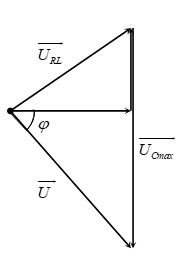
\includegraphics[scale=0.9]{../figs/VN12-PH-19-P-013-1-1.jpg}
		\end{center}
		
		+ Khi $C$ biến thiên để $U_C$  cực đại thì điện áp hai đầu đoạn mạch vuông pha với điện áp hai đầu đoạn mạch $RL$.
		
		+ Từ hình vẽ, ta có: 
		
		$$U^2 = U_{C\text{max}} (U_{C\text{max}} - U_L)  \Rightarrow 100^2  = U_{C\text{max}} (U_{C\text{max}} -\text{97,5}) \Rightarrow U_{C\text{max}} =160\ \text{V}$$
		$$\sin \varphi = \dfrac{U_C- U_L}{U} = \text{0,625} \Rightarrow \varphi = \text{0,22}  \pi$$
		Vậy điện áp hai đầu điện trở sớm pha hơn điện áp hai đầu đoạn mạch một góc $\text{0,22}  \pi$ rad.
		
	}
		\item \mkstar{3}
	
	\cauhoi{Đặt điện áp $u =160\sqrt 2\cos 100\pi t\ \text{V}$ vào hai đầu đoạn mạch mắc nối tiếp gồm điện trở $R=40\sqrt 3\ \Omega$ tụ điện và cuộn cảm thuần có độ tự cảm $L$ thay đổi được. Điều chỉnh độ tự cảm đến giá trị $L=L_0$ để điện áp hiệu dụng hai đầu cuộn cảm đạt giá trị cực đại và bằng 320 V. Biểu thức cường độ dòng điện trong mạch khi đó là
		\begin{mcq}(2)
			\item $i = 2\cos \left(100\pi t -\dfrac{\pi}{3}\right)\ \text{A}$.
			\item $i = 4\cos \left(100\pi t -\dfrac{\pi}{3}\right)\ \text{A}$.
			\item $i = 4\sqrt 2\cos \left(100\pi t -\dfrac{\pi}{6}\right)\ \text{A}$.
			\item $i = 2\sqrt 2\cos \left(100\pi t -\dfrac{\pi}{6}\right)\ \text{A}$.
		\end{mcq}
}	
		\loigiai{
			\textbf{Đáp án: D.}
			
			$$U_{L_\text{max}} =\dfrac{U}{L} \sqrt R^2 +Z^2_C \Leftrightarrow Z_C =120\ \Omega$$.
			$$Z_L = \dfrac{R^2+Z^2_C}{Z_C} =160\ \Omega \Rightarrow \bar{i} = \dfrac{\vec{u}}{\bar{Z}} = 2\sqrt 2 \angle  \dfrac{\pi}{6} $$.
			
			}
\item \mkstar{3}

\cauhoi{Mạch xoay chiều $R,L,C$ nối tiếp có $R=50\ \Omega$; $L=2/ \pi \,\text{H}$; $u=220\sqrt 2 \cos (100\pi t)\,\text{(V)}$. Tụ điện có $C$ thay đổi được. Xác định $C$ để điện áp cùng pha với cường độ dòng điện
	
	\begin{mcq}(2)
		\item $C=10^{-4}/{2\pi}\ \si{\farad}$.
		\item $C=10^{-3}/{2\pi}\ \si{\farad}$.
		\item $C=10^{-2}/{2\pi}\ \si{\farad}$.
		\item $C=10^{-4}/{4\pi}\ \si{\farad}$.
		
	\end{mcq}
}	
\loigiai{
	\textbf{Đáp án: A.}
	
	Điện áp cùng pha với dòng điện nên có hiện tượng cộng hưởng.
	
	$Z_L=Z_C \Rightarrow C=\dfrac {1}{\omega ^2 L}=C=10^{-4}/{2\pi}\ \si{\farad}.$
	
}	
\item \mkstar{3}

\cauhoi{Một mạch $RLC$ mắc nối tiếp trong đó $R=\SI{120}{\ohm}$, $L=\dfrac{2}{\pi}\,\text{H}$ và $C=\dfrac{2}{\pi}\cdot 10^{-4}\,\si{\farad}$, nguồn có tần số $f$ thay đổi được. Để $i$ sớm pha hơn $u$, giá trị của $f$ cần thỏa mãn:
	\begin{mcq}(2)
		\item $f>\SI{12.5}{Hz}$.
		\item $f\geq\SI{12.5}{Hz}$.
		\item $f<\SI{12.5}{Hz}$.
		\item $f<\SI{25}{Hz}$.
	\end{mcq}
}	
\loigiai{
	\textbf{Đáp án: D.}
	
	Với $i$ sớm pha hơn $u$ thì $\tan\varphi<0$ từ đó ta suy ra công thức tính $f$.
	
}	
	%%%%%%%%%%%%%%CÂU5%%%%%%%%%%
\item \mkstar{3}

\cauhoi{Mạch $RLC$ nối tiếp có $R=\SI{100}{\ohm}$, $L=2\sqrt{3}/\pi\,\text{H}$.Hiệu điện thế xoay chiều đặt vào đoạn mạch có biểu thức $u=U_0\cos2\pi ft$, $f$ thay đổi được. Khi $f=\SI{50}{Hz}$ thì $i$ trễ pha $\pi/3$ so với $u$. Để $i$ cùng pha với $u$ thì $f$ có giá trị là
	\begin{mcq}(4)
		\item $\SI{100}{Hz}$.
		\item $\SI{40}{Hz}$.
		\item $\SI{35,35}{Hz}$.
		\item $\SI{50}{Hz}$.
	\end{mcq}
}	
	\loigiai{
		\textbf{Đáp án: C.}
		
		Khi $f=\SI{50}{Hz}$ thì $\omega=100\pi\,\textrm{rad/s}$. Dung kháng là $Z_L=200\sqrt{3}\,\Omega.$
		
		Để mạch có $u$ và $i$ cùng pha thì có hiện tượng cộng hưởng nên $f=\dfrac{1}{2\pi\sqrt{LC}}=\SI{35,35}{Hz}$.
		
		}


%%%%%%%%%%%%%%CÂU20%%%%%%%%%%
		\item \mkstar{3}
	
	\cauhoi{Đặt một điện áp xoay chiều $u = U_0\cos \omega t$  vào hai đầu đoạn mạch AB  theo tứ tự gồm điện trở  $R=90\ \Omega$, cuộn dây không thuần cảm có điện trở  $r=10\ \Omega$ và tụ điện có điện dung $C$  thay đổi được. M  là điểm nối giữa điện trở $R$  và cuộn dây. Khi $C= C_1$  thì điện áp hiệu dụng hai đầu đoạn mạch MB  đạt giá trị cực tiểu bằng $U_1$ ; khi $C=C_2 =\dfrac{C_1}{2}$ thì điện áp hiệu dụng trên tụ điện đạt giá trị cực đại bằng $U_2$ . Tỉ số $\dfrac{U_2}{U_1}$ bằng
		\begin{mcq}(4)
			\item $5\sqrt 2$.
			\item $\sqrt 2$.
			\item $10\sqrt 2$.
			\item $9\sqrt 2$.
		\end{mcq}
}	
		\loigiai{
			\textbf{Đáp án: C.}
			
			Điện áp hiệu dụng hai đầu đoạn mạch MB: 
			
			$$U_\text{MB} = \dfrac{U\sqrt{r^2 + (Z_L-Z_C)^2}}{\sqrt{(R+r)^2 + (Z_L-Z_C)^2}} = \dfrac{U}{\sqrt{1+ \dfrac{R^2 +2Rr}{r^2 + (Z_L - Z_C)^2}}}$$
			$$\Rightarrow U_\text{MB min} =\dfrac{U}{\sqrt {1+\dfrac{R^2 +2Rr}{r^2}}} = \dfrac{U}{\sqrt 10}$$
			
			Khi $C=C_2=\text{0,5} C_1 \Rightarrow Z_{C_2} =2Z_{C_1} =2Z_L$ thì điện áp giữa hai tụ điện cực đại 
			
			$$Z_{C_2} =2Z_L = \dfrac{(R+r)^2 + Z_L^2}{Z_L}$$.
			$$U_2 =\dfrac{U}{R+r} \sqrt {(R+r)^2 + Z_L^2}$$ 
			Suy ra: $$Z_L =100\ \Omega; U_2 = \sqrt U$$
			
			Lập tỉ số $\dfrac{U_2}{U_1} = 10\sqrt 2$.			
			}
	
	%%%%%%%%%%%%%%CÂU2%%%%%%%%%%
	\item \mkstar{3}

\cauhoi{Cho đoạn mạch điện xoay chiều như hình vẽ, $U_\text{AB} =120\sqrt 2 \sin 100\pi t\ \text{V}$; cuộn dây thuần cảm, tụ điện có điện dung $C=\dfrac{10^{-4}}{\pi}\ \text{F}$. Điều chỉnh $L$ để Vôn kế có giá trị cực đại, khi đó số chỉ của Vôn kế là 200 V. Giá trị của $R$ là 
	\begin{center}
		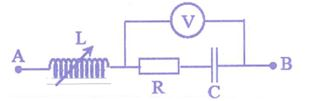
\includegraphics[scale=1]{../figs/VN12-PH-19-P-013-1-6.jpg}
	\end{center}
	\begin{mcq}(4)
		\item $100\ \Omega$.
		\item $60\ \Omega$.
		\item $75\ \Omega$.
		\item $150\ \Omega$.
	\end{mcq}
}	
	\loigiai{
		\textbf{Đáp án: C.}
		
		$Z_C =\dfrac{1}{\omega C} = 100\ \Omega$.
		
		Vôn kế đo hiệu điện thế hai đầu $RC$.
		
		Khi $L$ thay đổi, $U_{RC_\text{max}} \Leftrightarrow I_{\text{max}} $ suy ra trong mạch có cộng hưởng, ta có: $Z=R$.
		
		$$U_{RC_\text{max}} =\dfrac{U}{R} \sqrt{R^2 +Z^2_C} \Rightarrow R =75\ \Omega$$
\item \mkstar{4}

\cauhoi{Trong giờ thực hành, để đo điện dụng $C$ của một tụ điện, một học sinh mắc mạch điện theo sơ đồ như hình bên. Đặt vào hai đầu M,N một điện áp xoay chiều có giá trị hiệu dụng không đổi và tần số $50\ \textrm{Hz}$. Khi đóng khóa K vào chốt 1 thì số chỉ của ampe kế A là $I$. Chuyển khóa K sang chốt 2 thì số chỉ của ampe kế A là $2I$. Biết $R=680\ \Omega$. Bỏ qua điện trở của ampe kế và dây nối. Giá trị của $C$ là
	\begin{center}
		\includegraphics[scale=1.0]{../figs/chap3-6.jpg}
	\end{center}
	\begin{mcq}(2)
		\item $\text{9,36}\cdot 10^{-6}\ \textrm{F}$.
		\item $\text{4,68}\cdot 10^{-6}\ \textrm{F}$.
		\item $\text{18,73}\cdot 10^{-6}\ \textrm{F}$.
		\item $\text{2,34}\cdot 10^{-6}\ \textrm{F}$.
	\end{mcq}		
}		
\loigiai{
	\textbf{Đáp án: A.}
	
		Trường hợp đóng khóa K vào chốt 1, mạch điện gồm có 1 điện trở $R$ mắc vào nguồn điện. 
	Số chỉ của ampe kế cho biết giá trị của cường độ dòng điện hiệu dụng toàn mạch:
	
	$$I=\frac{U}{R}.$$
	Trường hợp đóng khóa K vào chốt 2, mạch điện gồm có 1 tụ điện $C$ mắc vào nguồn điện.
	Số chỉ của ampe kế cho biết giá trị của cường độ dòng điện hiệu dụng toàn mạch:
	
	$$2I=\frac{U}{Z_C}.$$
	
	Từ hai phương trình trên, ta được: 
	
	
	$$\frac {1}{2}=\frac {Z_C}{R} \\ \Leftrightarrow Z_C = \frac {R}{2} \\ \Leftrightarrow \frac {1}{\omega C}= \frac {R}{2} \\ \Leftrightarrow C = \frac {2}{\omega R}=\frac {2}{2\pi fR} \approx \text{9,36}\cdot 10^{-6}\ \textrm{F}.$$
	
}		
		}
	\item \mkstar{3}
	
	\cauhoi{Mạch điện xoay chiều $RLC$ mắc nối tiếp gồm điện trở thuần $R=\SI{10}{\ohm}$, cuộn cảm thuần có cảm kháng $Z_L=\SI{10}{\ohm}$ và tụ điện $C$ có dung kháng $Z_C=\SI{5}{\ohm}$ ứng với tần số $f$. Khi thay đổi tần số dòng điện đến giá trị $f'$ thì trong mạch có cộng hưởng điện. Tần số $f'$ liên hệ với $f$ theo biểu thức
		\begin{mcq}(4)
			\item $f'=f$.
			\item $f=\sqrt{2}f'$.
			\item $f'=\sqrt{2}f$.
			\item $f'=2f$.
		\end{mcq}
}		
		\loigiai{
			\textbf{Đáp án: B.}
			
			Ta có $Z_L=\omega_1L=\SI{10}{\ohm}$; $Z_C=\dfrac{1}{\omega_1 C}=\SI{5}{\ohm}$.
			
			Ta lại có
			$$\dfrac{Z_L}{Z_C}=\omega^2LC=2\Rightarrow \dfrac{\omega^2}{2}=\dfrac{1}{LC}=\omega'^2.$$
			
			Do đó $\omega=\sqrt{2}\omega'\Rightarrow f=\sqrt{2}f'$.
			
		}
	%%%%%%%%%%%%%%CÂU3%%%%%%%%%%
	\item \mkstar{4}
	
	\cauhoi{Đặt điện áp $u=U_0\cos \omega t$  ($U_0$, $\omega$  không đổi) vào đoạn mạch mắc nối tiếp gồm điện trở $R$, tụ điện có điện dung $C$ và cuộn cảm thuần có độ tự cảm $L$ thay đổi. Hình vẽ bên là đồ thị biểu diễn sự phụ thuộc của điện áp hiệu dụng $U_L$ giữa hai đầu cuộn cảm và hệ số công suất $\cos \varphi$  của đoạn mạch theo giá trị của độ tự cảm $L$. Giá trị của $U_0$ gần nhất với giá trị nào sau đây?
		\begin{center}
			\includegraphics[scale=0.9]{../figs/VN12-PH-19-P-013-1-2.jpg}
		\end{center}
		\begin{mcq}(4)
			\item 240 V.
			\item 165 V.
			\item 220 V.
			\item 185 V.
		\end{mcq}
	}
		\loigiai{
			\textbf{Đáp án: B.}
			
			Khi xảy ra cực đại của điện áp hiệu dụng trên cuộn cảm thuần $$Z_L = \dfrac{R^2+Z^2_C}{Z_C}$$
			
			Ta chuẩn hóa $R=1; Z_C = n \Rightarrow Z_L =\dfrac{1}{x} +x$.
			
			Hệ số công suất của mạch tương ứng $$\cos \varphi =\dfrac{R}{\sqrt{R^2 + (Z_L - Z_C)^2}} \Leftrightarrow \text{0,8} =\dfrac{1}{\sqrt {1+ \dfrac{1}{n^2}}} \Rightarrow n =\dfrac{4}{3}$$
			
			Kết hợp với $$U_{L\text{max}} = U\sqrt {1+ \left (\dfrac{Z_C}{R}\right)^2} \Rightarrow U = \dfrac{U_{L_\text{max}}}{\sqrt {1+\left (\dfrac{Z_C}{R}\right)^2 }} =120\ \text{V}$$
			
			Suy ra $U_0 =120\sqrt 2 \approx 170\ \text{V}$.
			
			
			}
	
	%%%%%%%%%%%%%%CÂU4%%%%%%%%%%

	\item \mkstar{4}
	
	\cauhoi{Cho mạch điện như hình vẽ, hai cuộn dây thuần cảm có độ tự cảm thay đổi, biết $R_2=5R_1$. Đặt vào hai đầu đoạn mạch một điện áp xoay $u =U\sqrt 2 \cos \omega t$ (với $U$ và $\omega$ không đổi). Điều chỉnh độ tự cảm của các cuộn dây (nhưng luôn thoả mãn $L_2=\text{0,8}L_1$) sao cho độ lệch pha giữa điện áp hai đầu đoạn mạch AM và MB lớn nhất, thì hệ số công suất của đoạn mạch khi đó bằng
		\begin{center}
			\includegraphics[scale=0.9]{../figs/VN12-PH-19-P-013-1-3.jpg}
		\end{center}
		\begin{mcq}(4)
			\item $\dfrac{8}{\sqrt {73}}$.
			\item 0,8.
			\item 0,6.
			\item $\dfrac{6}{\sqrt {73}}$.
		\end{mcq}
}	
		\loigiai{
			\textbf{Đáp án: A.}
			
			Giản đồ vec tơ như hình 
			\begin{center}
				\includegraphics[scale=0.9]{../figs/VN12-PH-19-P-013-1-4.jpg}
			\end{center}
			
			Ta có: $$\tan \alpha = \dfrac {\dfrac{Z_{Z_1}}{R_1} -\dfrac{Z_{L_2}}{R_2}}{1+ \dfrac{Z_{L_1} \cdot Z_{L_2}}{R_1R_2}}$$
			
			Đặt $x = \dfrac{Z_{L_1}}{R_1} \Rightarrow \tan \alpha = \dfrac{\text{0,84}x}{1+\dfrac{\text{0,8}}{5}x^2} = \dfrac {\text{0,84}}{\dfrac{1}{x} +\text{0,16}x}$.
			
			Áp dụng cosi suy ra $\tan \alpha \leq \dfrac{\text{0,84}}{2\sqrt{\text{0,16}}} =\text{1,05}.$
			
			$\Rightarrow \alpha_\text{max} =\text{0,81}$ và $x =\text{2,5}$ hay $Z_{L_1} =\text{2,5}R_1$; $Z_{L_2} =2R_1 \Rightarrow \tan \varphi = \dfrac{Z_{L_1} +Z_{L_2}}{R_1+R_2} =\dfrac{3}{4}$.
			
			$\Rightarrow \cos \varphi = \text{0,8}$.
			
			}
	
	%%%%%%%%%%%%%%CÂU6%%%%%%%%%%
	\item \mkstar{4}
	
	\cauhoi{Đặt một điện áp xoay chiều có giá trị hiệu dụng và tần số không đổi vào hai đầu đoạn mạch điện AB gồm biến trở $R$, tụ điện $C$ và cuộn dây không thuần cảm có độ tự cảm $L$, điện trở thuần $r$, ghép nối tiếp với nhau như hình vẽ.
		\begin{center}
			\includegraphics[scale=1]{../figs/VN12-PH-19-P-013-1-5.jpg}
		\end{center}
		Điều chỉnh R đến giá trị $60\ \Omega$ thì công suất tiêu thụ trên biến trở đạt cực đại, đồng thời tổng trở của đoạn mạch AB là số nguyên chia hết cho 45. Khi đó hệ số công suất của đoạn mạch MB có giá trị là
		
		\begin{mcq}(4)
			\item 0,375.
			\item 0,75.
			\item 0,125.
			\item 0,5.
		\end{mcq}
}	
		\loigiai{
			\textbf{Đáp án: C.}
			
			Giá trị của biến trở để công suất tiêu thụ trên biến trở là cực đại:
			
			$$R=R_0 = \sqrt{r^2 +(Z_L-Z_C)^2} = 60\ \Omega$$
			
			+ Tổng trở của mạch khi đó
			
			$$Z= \sqrt{(R_0 +r)^2 +(Z_L-Z_C)^2} = \sqrt {R_0^2 + 2R_0r +r^2 +(Z_L-Z_C)^2} \Rightarrow Z^2 = 60^2 +2 \cdot 60 r + 60^2 = (n \cdot 45)^2 \Rightarrow r =\dfrac{135}{8}n^2 -60$$
			
			+ Hệ số công suất của đoạn mạch MB:
			
			$$\cos \varphi_\text{MB} = \dfrac{r}{\sqrt {r^2 + (Z_L-Z_C)^2 }} = \dfrac{\dfrac{135}{8}n^2 -60}{60}$$
			$$ 0<\cos \varphi_\text{MB} <1 \Leftrightarrow \text{1,89}<n<\text{2,7}$$
			
			$n=2$ suy ra $\cos \varphi_\text{MB} =\text{0,125}$. 
			
			}
	
	%%%%%%%%%%%%%%CÂU7%%%%%%%%%%

	
	%%%%%%%%%%%%%%CÂU8%%%%%%%%%%
	\item \mkstar{4}
	
	\cauhoi{Cho mạch điện như hình vẽ, cuộn dây thuần cảm. Điện áp hai đầu đoạn mạch có biểu thức $u= U\sqrt 2\cos 2\pi f t\ \text{V}$  với $U$ không đổi nhưng $f$ có thể thay đổi được. Ta có đồ thị biểu diễn sự phụ thuộc của công suất tiêu thụ trên mạch theo $R$ là đường liền nét khi $f=f_1$  và là đường đứt nét khi $f=f_2$. Giá trị của $P_\text{max}$  gần nhất với giá trị nào sau đây?
		\begin{center}
			\includegraphics[scale=1.1]{../figs/VN12-PH-19-P-013-1-7.jpg}
		\end{center}
		\begin{mcq}(4)
			\item 280 W.
			\item 140 W.
			\item 130 W.
			\item 260 W.
		\end{mcq}
}		
		\loigiai{
			\textbf{Đáp án: C.}
			
			+	$f=f_1$: Công suất cực đại của mạch khi $R_0 =120 = |Z_{L_1} - Z_{C_1}|.$
			
			Khi đó: $$P_{\text{max}_1} = \dfrac{U^2}{2|Z_{L_1} - Z_{C_1}|} \Rightarrow 100 =\dfrac{U^2}{2 \cdot 120} \Rightarrow U = 40\sqrt {15} \ \text{V}$$
			
			+ $f=f_2$: khi $R=200\ \Omega$ thì công suất tiêu thụ của mạch là 100 W.
			
			$$\Rightarrow 100 = \dfrac{(40\sqrt{15})^2}{200^2 + (Z_{L_2}-Z_{C_2})^2} \cdot 200 \Rightarrow |Z_{L_2}-Z_{C_2}| =40\sqrt 5.$$
			
			Khi đó: $P_\text{max} = P_{\text{max}_2} = \dfrac{U^2}{2|Z_{L_2}-Z_{C_2}|} =60\sqrt 5 \approx \text{134,16}\ \text{W}$.
			
			
			}
	
	%%%%%%%%%%%%%%CÂU9%%%%%%%%%%
	\item \mkstar{4}
	
	\cauhoi{Đặt vào hai đầu đoạn mạch $RLC$ mắc nối tiếp một điện áp xoay chiều có giá trị hiệu dụng và tần số không đổi. Biết $R$ không đổi, cuộn thuần cảm có độ tự cảm $L$ không đổi, điện dung của tụ điện thay đổi được. Khi điện dung $C=C_1$  và $C=C_2$  thì điện áp hiệu dụng hai đầu tụ điện có cùng giá trị, khi $C=C_1$  thì điện áp u hai đầu đoạn mạch trễ pha hơn $i$ một góc $\dfrac{\pi}{6}$. Khi $C=C_2$  thì điện áp $u$ ở hai đầu đoạn mạch trễ pha hơn $i$ một góc $\dfrac{5\pi}{12}$. Khi $C=C_0$  thì điện áp hiệu dụng hai đầu tụ điện đạt giá trị cực đại là $U_{C_\text{max}} = 186\ \text{V}$, đồng thời khi đó điện áp hiệu dụng hai đầu $R$ có giá trị gần nhất với giá trị nào sau đây?
		\begin{mcq}(4)
			\item 200 V.
			\item 100 V.
			\item 180 V.
			\item 150 V.
		\end{mcq}
}		
		\loigiai{
		\textbf{Đáp án: B.}
			
			+ Với $\varphi_1, \varphi_2$ và $\varphi_0$ là độ lệch pha giữa $u$ và $i$ ứng với $C_1; C_2; C_0$.
			
			Ta có: $\varphi_1 + \varphi_2 =2\varphi_0 \Rightarrow \varphi_0 = - \text{52,5}^\circ$.
			
			+ Khi $C=C_0$ điện áp hiệu dụng trên tụ cực đại thì $u_{RL}$ vuông pha với $u$.
			\begin{center}
				\includegraphics[scale=0.9]{../figs/VN12-PH-19-P-013-1-8.jpg}
			\end{center}
			+ Từ hình vẽ, ta có: 
			
			$$U=U_{C_\text{max}} \sin |\varphi_0|$$
			$$U_R =U \cos |\varphi_0|$$.
			$$\Rightarrow U_R = \dfrac{U_{C_\text{max}}}{2} \sin 2\varphi_0 = 89\ \text{V}$$
			
			
			}
	
	%%%%%%%%%%%%%%CÂU10%%%%%%%%%%
	\item \mkstar{4}
	
	\cauhoi{Cho mạch điện như hình vẽ: $R=100\ \Omega$, cuộn dây thuần cảm có $L=\dfrac{1}{\pi}\ \text{H}$. Khi mắc nguồn điện xoay chiều (100 V - 50 Hz) vào hai điểm A, C thì số chỉ của hai vôn kế như nhau và bằng
		
		\begin{center}
			\includegraphics[scale=1.1]{../figs/VN12-PH-19-P-013-1-9.jpg}
		\end{center}
		\begin{mcq}(4)
			\item 141 V.
			\item 100 V.
			\item 200 V.
			\item 150 V.
		\end{mcq}
}	
		\loigiai{
		\textbf{Đáp án: A.}
			
			Sau khi mắc nguồn điện xoay chiều tại hai điểm A và C, mạch điện được vẽ lại như hình trên. 
			
			\begin{center}
				\includegraphics[scale=1.1]{../figs/VN12-PH-19-P-013-1-10.jpg}
			\end{center}
			
			$$U_1 = \sqrt {U_C^2 +U_R^2};U_2 = \sqrt {U_L^2 +U_R^2} (\text{mà} U_1 =U_2) \Rightarrow U_C=U_L.$$ 
			
			Suy ra Mạch đang có cộng hưởng điện nên $U_R=U$.
			$$\Rightarrow I =\dfrac{U}{R} =1\ \text{A}$$.
			$$Z_L = \omega L = 100\ \Omega \Rightarrow U_L = IZ_L = 100\ \Omega$$.
			$$U_{V_1} = U_{V_2} =\sqrt {U^2_L +U^2_R} =100\sqrt 2\ \Omega$$.
		}
\end{enumerate}
\loigiai{\textbf{Đáp án}
	\begin{center}
		\begin{tabular}{|m{2.8em}|m{2.8em}|m{2.8em}|m{2.8em}|m{2.8em}|m{2.8em}|m{2.8em}|m{2.8em}|m{2.8em}|m{2.8em}|}
			\hline
			1. B & 2. A & 3. B & 4. C & 5. D & 6. A  & 7. C  & 8. C & 9. A & 10. B\\
			\hline
			11. A & 12. C & 13. A & 14. A & 15. B & 16. C  & 17. C  & 18. C & 19. A & 20. C\\
			\hline
			21. B & 22. A & 23. A & 24. D & 25. A & 26. B  & 27. A  & 28. D & 29. A & 30. D\\
			\hline
			31. C & 32. C & 33. C & 34. A & 35. B & 36. B  & 37. A  & 38. C & 39. C & 40. B\\
			\hline
		\end{tabular}
\end{center}}
\stopcontents[mychapters]
\setcounter{mychapter}{14}
\mychapter{Công suất tiêu thụ của mạch điện xoay chiều. Hệ số công suất}
\startcontents[mychapters]
\printcontents[mychapters]{}{0}{\setcounter{tocdepth}{1}}
\begin{enumerate}[label=\bfseries Câu \arabic*:]
	
	
	%%%%%%%%%%%%%%CÂU2%%%%%%%%%%
	\item \mkstar{1}
	
	\cauhoi{Phát biểu nào sau đây là \textbf{không} đúng?
		\begin{mcq}(1)
			\item Công suất của dòng điện xoay chiều phụ thuộc vào công suất hao phí trên đường dây tải điện.
			\item Công suất của dòng điện xoay chiều phụ thuộc vào hiệu điện thế hiệu dụng giữa hai đầu đoạn mạch.
			\item Công suất của dòng điện xoay chiều phụ thuộc vào cường độ dòng điện hiệu dụng trong mạch.
			\item Công suất của dòng điện xoay chiều phụ thuộc vào bản chất của mạch điện và tần số dòng điện trong mạch.
		\end{mcq}
	}	
	\loigiai{
		\textbf{Đáp án: A.}
		
		Công suất của dòng điện xoay chiều được tính theo công thức $P=UI\cos\varphi$. Suy ra công suất của dòng điện xoay chiều phụ thuộc vào cường độ dòng điện hiệu dụng I trong mạch, điện áp hiệu dụng U giữa hai đầu đoạn mạch, bản chất của mạch điện và tần số dòng điện trong mạch (đặc trưng bởi độ lệch pha).
		
	}
	
	%%%%%%%%%%%%%%CÂU3%%%%%%%%%%

	
	%%%%%%%%%%%%%%CÂU4%%%%%%%%%%
	\item \mkstar{1}
	
	\cauhoi{Công suất của dòng điện xoay chiều trên đoạn mạch RLC nối tiếp \textbf{không} phụ thuộc vào đại lượng nào sau đây?
		\begin{mcq}
			\item Hiệu điện thế cực đại giữa hai đầu đoạn mạch.
			\item Cường độ hiệu đụng của dòng điện qua mạch.
			\item Độ lệch pha giữa dòng điện và hiệu điện thế giữa hai bản tụ.
			\item Tỉ số giữa điện trở thuần và tổng trở của mạch.
		\end{mcq}
	}	
	\loigiai{
		\textbf{Đáp án: C.}
		
		Độ lệch pha giữa dòng điện và điện áp giữa hai đầu tụ điện luôn là $\dfrac{\pi}{2}$.
		
	}
	
	%%%%%%%%%%%%%%CÂU5%%%%%%%%%%

	
	%%%%%%%%%%%%%%CÂU7%%%%%%%%%%
	\item \mkstar{1}
	
	\cauhoi{Trong các dụng cụ tiêu thụ điện như quạt, tủ lạnh, động cơ, người ta năng cao hệ số công suất nhằm
		\begin{mcq}(2)
			\item tăng cường độ dòng điện.
			\item tăng công suất tiêu thụ.
			\item giảm cường độ dòng điện.
			\item giảm công suất tiêu thụ.
		\end{mcq}
	}	
	\loigiai{
		\textbf{Đáp án: C.}
		
		Trong các dụng cụ tiêu thụ điện như quạt, tủ lạnh, động cơ, người ta năng cao hệ số công suất nhằm giảm cường độ dòng điện, giảm hao phí tỏa nhiệt và nâng cao hiệu suất.
		
	}
	
	%%%%%%%%%%%%%%CÂU8%%%%%%%%%%
	
	%%%%%%%%%%%%%%CÂU9%%%%%%%%%%
\item \mkstar{2}

\cauhoi{Công suất của dòng điện xoay chiều trên một đoạn mạch $RLC$ nối tiếp nhỏ hơn tích $UI$ là do
	\begin{mcq}
		\item một phần điện năng tiêu thụ trong tụ điện.
		\item trong cuộn dây có dòng điện cảm ứng.
		\item điện áp giữa hai đầu đoạn mạch và cường độ dòng điện lệch pha không đổi với nhau.
		\item có hiện tượng cộng hưởng điện trên đoạn mạch.
	\end{mcq}
}
	\loigiai{
		\textbf{Đáp án: C.}
		
		Công suất của dòng điện xoay chiều trên một đoạn mạch $RLC$ nối tiếp nhỏ hơn tích $UI$ là do điện áp giữa hai đầu đoạn mạch và cường độ dòng điện lệch pha không đổi với nhau.
		
		}


%%%%%%%%%%%%%%CÂU3%%%%%%%%%%
\item \mkstar{2}

\cauhoi{Một điện áp xoay chiều được đặt vào hai đầu một điện trở thuần. Giữ nguyên giá trị hiệu dụng, thay đổi tần số của điện áp. Công suất toả nhiệt trên điện trở
	\begin{mcq}
		\item tỉ lệ thuận với bình phương của tần số.
		\item tỉ lệ thuận với tần số.
		\item tỉ lệ nghịch với tần số.
		\item không phụ thuộc vào tần số.
	\end{mcq}
}	
	\loigiai{
		\textbf{Đáp án: D.}
		
		$\calP=UI\cos\varphi=I^2R$.
		
		}


%%%%%%%%%%%%%%CÂU4%%%%%%%%%%
\item \mkstar{2}

\cauhoi{Đoạn mạch điện nào sau đây có hệ số công suất lớn nhất?
	\begin{mcq}
		\item Điện trở thuần $R_1$ nối tiếp với điện trở thuần $R_2$.
		\item Điện trở thuần $R$ nối tiếp với cuộn cảm $L$.
		\item Điện trở thuần $R$ nối tiếp với tụ điện $C$.   
		\item Cuộn cảm $L$ nối tiếp với tụ điện $C$.
	\end{mcq}
}	
	\loigiai{
		\textbf{Đáp án: A.}
		
		$\cos\varphi=\dfrac{R}{Z}$.
		
		}




%%%%%%%%%%%%%%CÂU5%%%%%%%%%%
\item \mkstar{2}

\cauhoi{Công suất tức thời của dòng điện xoay chiều
	\begin{mcq}
		\item luôn biến thiên với tần số bằng hai lần tần số của dòng điện.
		\item có giá trị trung bình biến thiên theo thời gian.
		\item không thay đổi theo thời gian, tính bằng công thức $\calP=UI\cos\varphi$.
		\item luôn biến thiên cùng pha, cùng tần số với dòng điện.
	\end{mcq}
}	
	\loigiai{
		\textbf{Đáp án: A.}
		
		Công suất tức thời của dòng điện xoay chiều luôn biến thiên với tần số bằng hai lần tần số của dòng điện.
		
		}


%%%%%%%%%%%%%%CÂU6%%%%%%%%%%
\item \mkstar{2}

\cauhoi{Trong mạch điện xoay chiều không phân nhánh, điện áp giữa hai đầu đoạn mạch và cường độ dòng điện trong mạch lần lượt là $u=100\cos 100\pi t\,\text{V}$ và $i=100\cos\left(100\pi t+\dfrac{\pi}{3}\right)\,\text{mA}$. Công suất tiêu thụ trong mạch là
	\begin{mcq}(4)
		\item $\SI{5000}{\watt}$.
		\item $\SI{2500}{\watt}$.
		\item $\SI{50}{\watt}$.
		\item $\SI{2,5}{\watt}$.
	\end{mcq}
}	
	\loigiai{
		\textbf{Đáp án: D.}
		
		$\calP=UI\cos\varphi=\SI{2,5}{\watt}.$
		
		}


%%%%%%%%%%%%%%CÂU7%%%%%%%%%%
\item \mkstar{2}

\cauhoi{Đặt một điện áp xoay chiều $\SI{100}{V}-\SI{50}{Hz}$ vào hai đầu một cuộn dây có điện trở là $r=\SI{10}{\ohm}$ thì dòng điện chạy qua cuộn dây lệch pha $\dfrac{\pi}{3}$ so với điện áp đó. Công suất tiêu thụ của cuộn dây là
	\begin{mcq}(4)
		\item $\SI{600}{\watt}$.
		\item $\SI{500}{\watt}$.
		\item $\SI{250}{\watt}$.
		\item $\SI{125}{\watt}$.
	\end{mcq}
}	
	\loigiai{
		\textbf{Đáp án: C.}
		
		$\calP=I^2R=UI\cos\varphi=\dfrac{U^2}{R}\cos^2\varphi=\SI{250}{\watt}$.
		
		}


%%%%%%%%%%%%%%CÂU8%%%%%%%%%%


%%%%%%%%%%%%%%CÂU10%%%%%%%%%%

	%%%%%%%%%%%%%%CÂU13%%%%%%%%%%
	\item \mkstar{2}
	
	\cauhoi{Đặt vào hai đầu đoạn mạch $RLC$ mắc nối tiếp một hiệu điện thế dao động điều hòa có biểu thức $u=220\sqrt{2}\cos\omega t\,\text{V}$. Biết điện trở thuần của mạch có giá trị là $\SI{100}{\ohm}$. Khi $\omega$ thay đổi thì công suất tiêu thụ cực đại của mạch có giá trị là
		\begin{mcq}(4)
			\item $\SI{440}{\watt}$.
			\item $\SI{484}{\watt}$.
			\item $\SI{220}{\watt}$.
			\item $\SI{242}{\watt}$.
		\end{mcq}
	}	
	\loigiai{
		\textbf{Đáp án: B.}
		
		Khi $\omega$ thay đổi để $P_\text{max}$ thì hiện tượng cộng hưởng xảy ra
		$$P_\text{max}=\dfrac{U^2}{R}=\SI{484}{\watt}.$$
		
	}
\item \mkstar{2}

\cauhoi{Đặt một điện áp xoay chiều vào hai đầu đoạn mạch $RLC$ nối tiếp có $R$ thay đổi thì thấy khi $R=\SI{30}{\ohm}$ và $R=\SI{120}{\ohm}$ thì công suất tỏa nhiệt trên đoạn mạch không đổi. Để công suất đó đạt cực đại thì giá trị $R$ phải là
	\begin{mcq}(4)
		\item $\SI{150}{\ohm}$.
		\item $\SI{24}{\ohm}$.
		\item $\SI{90}{\ohm}$.
		\item $\SI{60}{\ohm}$.
	\end{mcq}
}	
\loigiai{
	\textbf{Đáp án: D.}
	
	$R\sqrt{R_1R_2}=\SI{60}{\ohm}.$
	
}


%%%%%%%%%%%%%%CÂU9%%%%%%%%%%
\item \mkstar{2}

\cauhoi{Một đoạn mạch nối tiếp gồm một cuộn dây và một tụ điện. Hiệu điện thế hiệu dụng giữa hai đầu đoạn mạch, giữa hai đầu cuộn dây, hai đầu tụ điện đều bằng nhau. Tìm hệ số công suất $\cos\varphi$ của mạch.
	\begin{mcq}(4)
		\item 0,5.
		\item $\dfrac{\sqrt{3}}{2}$.
		\item $\dfrac{\sqrt{2}}{2}$.
		\item $\dfrac{1}{4}$.
	\end{mcq}
}	
\loigiai{
	\textbf{Đáp án: B.}
	
	Ta đặt $U=U_\text{d}=U_C=1$.
	
	Ta có $U^2=U_r^2+(U_L-U_C)^2\Rightarrow 1=U_r^2+(U_L-1)^2$.
	
	và $U_\text{d}^2=U_r^2+U_L^2\Rightarrow 1=U_r^2+U_L^2$.
	
	Từ đó ta suy ra $U_L=0,5$, $U_r=\dfrac{\sqrt{3}}{2}$.
	
	Hệ số công suất $\cos\varphi$ của mạch là $\cos\varphi=\dfrac{U_r}{U}=\dfrac{\sqrt{3}}{2}$.
	
}

	%%%%%%%%%%%%%%CÂU15%%%%%%%%%%
	\item \mkstar{3}
	
	\cauhoi{Cho đoạn mạch không phân nhánh $RLC$, $R=\SI{80}{\ohm}$,cuộn dây có điện trở trong $\SI{20}{\ohm}$ và độ tự cảm $L=\SI{0,318}{H}$, tụ điện có điện dung $\SI{15,9}{\micro\farad}$. Đặt vào hai đầu mạch điện một dòng điện xoay chiều có tần số $f$ thay đổi được có hiệu điện thế hiệu dụng là $\SI{200}{V}$.Khi công suất trên toàn mạch đạt giá trị cực đại thì giá trị của $f$ và $\calP$ bằng bao nhiêu?
		\begin{mcq}(2)
			\item $\SI{70,78}{Hz}$ và $\SI{400}{\watt}$.
			\item $\SI{70,78}{Hz}$ và $\SI{500}{\watt}$.
			\item $\SI{444,7}{Hz}$ và $\SI{2000}{\watt}$.
			\item $\SI{31,48}{Hz}$ và $\SI{400}{\watt}$.
		\end{mcq}
	}	
	\loigiai{
		\textbf{Đáp án: A.}
		
		Khi cường độ dòng điện trong mạch cực đại thì cộng hưởng điện xảy ra. Khi đó cường độ dòng điện cực đại là
		$$I=\dfrac{U}{R+r}=\SI{2}{A}.$$
		
		Tần số dòng điện là
		$$f=\dfrac{\omega}{2\pi}=\dfrac{1}{2\pi\sqrt{LC}}=\SI{70,78}{Hz}.$$
		
		Công suất cực đại là $P=I^2(R+r)=\SI{400}{\watt}$.
		
	}
	
	%%%%%%%%%%%%%%CÂU16%%%%%%%%%%
	\item \mkstar{3}
	
	\cauhoi{Đặt vào hai đầu đoạn mạch $RLC$ mắc nối tiếp một hiệu điện thế dao động điều hòa có biểu thức $u=220\cos\omega t\, \text{V}$. Khi $\omega$ thay đổi công suất tiêu thụ cực đại của mạch là $\SI{484}{\watt}$. Khi đó điện trở thuần của mạch là
		\begin{mcq}(4)
			\item $R=\SI{50}{\ohm}$.
			\item $R=\SI{750}{\ohm}$.
			\item $R=\SI{150}{\ohm}$.
			\item $R=\SI{100}{\ohm}$.
		\end{mcq}
	}	
	\loigiai{
		\textbf{Đáp án: A.}
		
		Khi $\omega$ thay đổi để công suất cực đại thì có cộng hưởng. Điện trở thuần của mạch là
		$$R=\dfrac{U^2}{P}=\SI{50}{\ohm}.$$
		
	}
\item \mkstar{3}

\cauhoi{Một đoạn mạch xoay chiều gồm cuộn dây có điện trở $R$, độ tự cảm $L$ nối tiếp với một tụ điện có điện dung $C$ đặt dưới điện áp xoay chiều có giá trị hiệu dụng ổn định. Cường độ dòng điện qua mạch là $i_1=3\cos100\pi t\,\text{A}$. Nếu tụ điện bị nối tắt thì cường độ dòng điện qua mạch là $i_2=3\cos\left(100\pi t+\dfrac{\pi}{3}\right)\,\text{A}$. Hệ số công suất trong hai trường hợp trên lần lượt là
	\begin{mcq}(2)
		\item $\cos\varphi_1=1$, $\cos\varphi_2=\dfrac{1}{2}$.
		\item $\cos\varphi_1=\cos\varphi_2=\dfrac{\sqrt{3}}{2}$.
		\item $\cos\varphi_1=\cos\varphi_2=\dfrac{3}{4}$.
		\item $\cos\varphi_1=\cos\varphi_2=\dfrac{1}{2}$.
	\end{mcq}
}	
\loigiai{
	\textbf{Đáp án: B.}
	
	Lúc đầu mạch là $RLC$ thì dòng điện $i_1=3\cos100\pi t\,\text{A}$.
	
	Khi nối tắt tụ điện thì mạch chỉ còn $RL$ cường độ dòng điện là $i_2=3\cos\left(100\pi t+\dfrac{\pi}{3}\right)\,\text{A}$.
	
	Ta thấy $I_{01}=I_{02}=\SI{3}{A}$. Do đó $Z_{RLC}=Z_{RL}$. Từ đó suy ra $\cos\varphi_1=\cos\varphi_2=\dfrac{\sqrt{3}}{2}$.	
	
}	
	%%%%%%%%%%%%%%CÂU17%%%%%%%%%%
	\item \mkstar{3}
	
	\cauhoi{Đoạn mạch xoay chiều gồm điện trở $R$, tụ điện có điện dung $C$ thay đổi được, cuộn dây có độ tự cảm $L=\dfrac{1}{\pi}\,\text{H}$ và điện trở $r=\SI{20}{\ohm}$ mắc nối tiếp. Đặt vào hai đầu đoạn mạch điện áp xoay chiều có giá trị hiệu dụng $U=\SI{60}{V}$ và tần số $f=\SI{50}{Hz}$. Điều chỉnh điện dung tụ điện đến giá trị $C_1$ thì công suất tiêu thụ trên mạch đạt cực đại và bằng $\SI{30}{\watt}$. Điện trở $R$ và điện dung $C_1$ có giá trị là
		\begin{mcq}(2)
			\item $R=\SI{120}{\ohm}$; $C_1=\dfrac{10^4}{2\pi}\,\text{F}$.
			\item $R=\SI{120}{\ohm}$; $C_1=\dfrac{10^4}{\pi}\,\text{F}$.
			\item $R=\SI{100}{\ohm}$; $C_1=\dfrac{10^4}{2\pi}\,\text{F}$.
			\item $R=\SI{100}{\ohm}$; $C_1=\dfrac{10^4}{\pi}\,\text{F}$.
		\end{mcq}
	}	
	\loigiai{
		\textbf{Đáp án: D.}
		
		Khi $C$ thay đổi để công suất cực đại thì xảy ra hiện tượng cộng hưởng nên $C=\dfrac{10^4}{\pi}\,\text{F}$.
		
		Điện trở là $R=\dfrac{U^2}{P_\text{max}}-r=\SI{100}{\ohm}$.
		
	}

	\item \mkstar{3}
	
	\cauhoi{Cho mạch điện gồm $R$, $L$, $C$ mắc nối tiếp. Biết $R=\SI{30}{\ohm}$, $R=\SI{0,4}{H}$, $C$ thay đổi được. Đặt vào hai đầu mạch điện một hiệu điện thế xoay chiều $u=120\cos(100t+\pi/2)\,\text{V}$. Khi $C=C_0$ thì công suất trong mạch đạt giá trị cực đại. Khi đó biểu thức điện áp giữa hai đầu điện trở là
		\begin{mcq}(2)
			\item $u_R=60\sqrt{2}\cos100t\,\text{V}$.
			\item $u_R=120\sqrt{2}\cos(100t+\pi/2)\,\text{V}$.
			\item $u_R=120\sqrt{2}\cos100t\,\text{V}$.
			\item $u_R=60\sqrt{2}\cos(100t+\pi/2)\,\text{V}$.
		\end{mcq}
	}	
	\loigiai{
		\textbf{Đáp án: B.}
		
		Ta có cảm kháng là $Z_L=\omega L=\SI{40}{\omega}$.
		
		Khi $C$ thay đổi để công suất tiêu thụ cực đại thì $Z_L=Z_C=\SI{40}{\ohm}$.
		
		Do đó $u_R$ cùng pha với $u$ nên $u_R=120\sqrt{2}\cos(100t+\pi/2)\,\text{V}$.
		
	}
	
	%%%%%%%%%%%%%%CÂU19%%%%%%%%%%

	%%%%%%%%%%%%%%CÂU3%%%%%%%%%%
	\item \mkstar{4}
	
	\cauhoi{Đặt điện áp $u=U_0\cos \omega t$  ($U_0$, $\omega$  không đổi) vào đoạn mạch mắc nối tiếp gồm điện trở $R$, tụ điện có điện dung $C$ và cuộn cảm thuần có độ tự cảm $L$ thay đổi. Hình vẽ bên là đồ thị biểu diễn sự phụ thuộc của điện áp hiệu dụng $U_L$ giữa hai đầu cuộn cảm và hệ số công suất $\cos \varphi$  của đoạn mạch theo giá trị của độ tự cảm $L$. Giá trị của $U_0$ gần nhất với giá trị nào sau đây?
		\begin{center}
			\includegraphics[scale=0.9]{../figs/VN12-PH-19-P-013-1-2.jpg}
		\end{center}
		\begin{mcq}(4)
			\item 240 V.
			\item 165 V.
			\item 220 V.
			\item 185 V.
		\end{mcq}
	}
	\loigiai{
		\textbf{Đáp án: B.}
		
		Khi xảy ra cực đại của điện áp hiệu dụng trên cuộn cảm thuần $$Z_L = \dfrac{R^2+Z^2_C}{Z_C}$$.
		
		Ta chuẩn hóa $R=1; Z_C = n \Rightarrow Z_L =\dfrac{1}{x} +x$.
		
		Hệ số công suất của mạch tương ứng $$\cos \varphi =\dfrac{R}{\sqrt{R^2 + (Z_L - Z_C)^2}} \Leftrightarrow \text{0,8} =\dfrac{1}{\sqrt {1+ \dfrac{1}{n^2}}} \Rightarrow n =\dfrac{4}{3}$$.
		
		Kết hợp với $$U_{L\text{max}} = U\sqrt {1+ \left (\dfrac{Z_C}{R}\right)^2} \Rightarrow U = \dfrac{U_{L_\text{max}}}{\sqrt {1+\left (\dfrac{Z_C}{R}\right)^2 }} =120\ \text{V}$$
		
		Suy ra $U_0 =120\sqrt 2 \approx 170\ \text{V}$.
		
		
	}
	
	%%%%%%%%%%%%%%CÂU4%%%%%%%%%%
	

	%%%%%%%%%%%%%%CÂU6%%%%%%%%%%
	\item \mkstar{4}
	
	\cauhoi{Đặt một điện áp xoay chiều có giá trị hiệu dụng và tần số không đổi vào hai đầu đoạn mạch điện AB gồm biến trở $R$, tụ điện $C$ và cuộn dây không thuần cảm có độ tự cảm $L$, điện trở thuần $r$, ghép nối tiếp với nhau như hình vẽ.
		\begin{center}
			\includegraphics[scale=1]{../figs/VN12-PH-19-P-013-1-5.jpg}
		\end{center}
		Điều chỉnh R đến giá trị $60\ \Omega$ thì công suất tiêu thụ trên biến trở đạt cực đại, đồng thời tổng trở của đoạn mạch AB là số nguyên chia hết cho 45. Khi đó hệ số công suất của đoạn mạch MB có giá trị là
		
		\begin{mcq}(4)
			\item 0,375.
			\item 0,75.
			\item 0,125.
			\item 0,5.
		\end{mcq}
	}	
	\loigiai{
		\textbf{Đáp án: C.}
		
		Giá trị của biến trở để công suất tiêu thụ trên biến trở là cực đại:
		
		$$R=R_0 = \sqrt{r^2 +(Z_L-Z_C)^2} = 60\ \Omega$$
		
		+ Tổng trở của mạch khi đó
		
		$$Z= \sqrt{(R_0 +r)^2 +(Z_L-Z_C)^2} = \sqrt {R_0^2 + 2R_0r +r^2 +(Z_L-Z_C)^2}$$
		$$\Rightarrow Z^2 = 60^2 +2 \cdot 60 r + 60^2 = (n \cdot 45)^2 \Rightarrow r =\dfrac{135}{8}n^2 -60$$
		
		+ Hệ số công suất của đoạn mạch MB:
		
		$$\cos \varphi_\text{MB} = \dfrac{r}{\sqrt {r^2 + (Z_L-Z_C)^2 }} = \dfrac{\dfrac{135}{8}n^2 -60}{60}$$
		$$ 0<\cos \varphi_\text{MB} <1 \Leftrightarrow \text{1,89}<n<\text{2,7}$$
		
		$n=2$ suy ra $\cos \varphi_\text{MB} =\text{0,125}$. 
		
	}
	
	%%%%%%%%%%%%%%CÂU7%%%%%%%%%%
	
	
	%%%%%%%%%%%%%%CÂU8%%%%%%%%%%
	\item \mkstar{4}
	
	\cauhoi{Cho mạch điện như hình vẽ, cuộn dây thuần cảm. Điện áp hai đầu đoạn mạch có biểu thức $u= U\sqrt 2\cos 2\pi f t\ \text{V}$  với $U$ không đổi nhưng $f$ có thể thay đổi được. Ta có đồ thị biểu diễn sự phụ thuộc của công suất tiêu thụ trên mạch theo $R$ là đường liền nét khi $f=f_1$  và là đường đứt nét khi $f=f_2$. Giá trị của $P_\text{max}$  gần nhất với giá trị nào sau đây?
		\begin{center}
			\includegraphics[scale=1.1]{../figs/VN12-PH-19-P-013-1-7.jpg}
		\end{center}
		\begin{mcq}(4)
			\item 280 W.
			\item 140 W.
			\item 130 W.
			\item 260 W.
		\end{mcq}
	}		
	\loigiai{
		\textbf{Đáp án: C.}
		
		+	$f=f_1$: Công suất cực đại của mạch khi $R_0 =120 = |Z_{L_1} - Z_{C_1}|.$
		
		Khi đó: $$P_{\text{max}_1} = \dfrac{U^2}{2|Z_{L_1} - Z_{C_1}|} \Rightarrow 100 =\dfrac{U^2}{2 \cdot 120} \Rightarrow U = 40\sqrt {15} \ \text{V}$$
		
		+ $f=f_2$: khi $R=200\ \Omega$ thì công suất tiêu thụ của mạch là 100 W.
		
		$$\Rightarrow 100 = \dfrac{(40\sqrt{15})^2}{200^2 + (Z_{L_2}-Z_{C_2})^2} \cdot 200 \Rightarrow |Z_{L_2}-Z_{C_2}| =40\sqrt 5.$$
		
		Khi đó: $P_\text{max} = P_{\text{max}_2} = \dfrac{U^2}{2|Z_{L_2}-Z_{C_2}|} =60\sqrt 5 \approx \text{134,16}\ \text{W}$.
		
		
	}
	
	%%%%%%%%%%%%%%CÂU9%%%%%%%%%%

\end{enumerate}
\loigiai{\textbf{Đáp án}
	\begin{center}
		\begin{tabular}{|m{2.8em}|m{2.8em}|m{2.8em}|m{2.8em}|m{2.8em}|m{2.8em}|m{2.8em}|m{2.8em}|m{2.8em}|m{2.8em}|}
			\hline
			1. A & 2. C & 3. C & 4. C & 5. D & 6. A  & 7. A  & 8. D & 9. C & 10. B\\
			\hline
			11. D & 12. B & 13. A & 14. A & 15. B & 16. D  & 17. B  & 18. B & 19. C & 20. C\\
			\hline
		\end{tabular}
\end{center}}
\stopcontents[mychapters]
\setcounter{mychapter}{15}
\mychapter{Truyền tải điện năng. Máy biến áp}
\startcontents[mychapters]
\printcontents[mychapters]{}{0}{\setcounter{tocdepth}{1}}
\begin{enumerate}[label=\bfseries Câu \arabic*:]
	
	
	%%%%%%%%%%%%%%CÂU2%%%%%%%%%%
	\item \mkstar{1}
	
	\cauhoi{Một máy biến áp có số vòng dây của cuộn sơ cấp lớn hơn số vòng dây của cuộn thứ cấp. Máy biến áp này có tác dụng
		\begin{mcq}
			\item tăng cường độ dòng điện, giảm điện áp.
			\item giảm cường độ dòng điện, tăng điện áp.
			\item tăng cường độ dòng điện, tăng điện áp.
			\item giảm cường độ dòng điện, giảm điện áp.
		\end{mcq}
}	
		\loigiai{
			\textbf{Đáp án: A.}
			
			Máy biến áp có số vòng cuộn sơ cấp lớn hơn số vòng cuộn thứ cấp là máy hạ áp và có tác dụng làm tăng cường độ dòng điện.
			
			}	
	
	%%%%%%%%%%%%%%CÂU2%%%%%%%%%%
	\item \mkstar{1}
	
	\cauhoi{Hoạt động của máy biến áp dựa trên
		\begin{mcq}(2)
			\item hiên tượng tự cảm.
			\item hiên tượng cảm ứng điện từ.
			\item từ trường quay.
			\item tác dụng của lực từ.
		\end{mcq}
}	
		\loigiai{
			\textbf{Đáp án: B.}
			
			Hoạt động của máy biến áp dựa trên hiên tượng cảm ứng điện từ.
			
			}
	
	%%%%%%%%%%%%%%CÂU3%%%%%%%%%%
	\item \mkstar{1}
	
	\cauhoi{Nguyên nhân chủ yếu gây ra sự hao phí năng lượng trong máy biến thế là do
		\begin{mcq}
			\item hao phí năng lượng dưới dạng nhiệt năng tỏa ra ở các cuộn sơ cấp và thứ cấp của máy biến thế.
			\item lõi sắt có từ trở và gây dòng Fu-cô.
			\item có sự thất thoát năng lượng dưới dạng bức xạ điện từ.
			\item Cả 3 ý kiến trên.
		\end{mcq}
}	
		\loigiai{
			\textbf{Đáp án: D.}
			
			Nguyên nhân chủ yếu gây ra sự hao phí năng lượng trong máy biến thế là do
			\begin{itemize}
				\item hao phí năng lượng dưới dạng nhiệt năng tỏa ra ở các cuộn sơ cấp và thứ cấp của máy biến thế.
				\item lõi sắt có từ trở và gây dòng Fu-cô.
				\item có sự thất thoát năng lượng dưới dạng bức xạ điện từ.
			\end{itemize}
			
			}
	
	%%%%%%%%%%%%%%CÂU4%%%%%%%%%%
	\item \mkstar{1}
	
	\cauhoi{Vai trò của máy biến thế trong truyền tải điện năng là
		\begin{mcq}
			\item giảm điện trở của dây dẫn trên đường truyền tải để giảm hao phí trên đường truyền tải.
			\item tăng hiệu điện thế truyền tải để giảm hao phí trên đường truyền tải.
			\item giảm hiệu điện thế truyền tải để giảm hao phí trên đường truyền tải.
			\item giảm sự thất thoát năng lượng dưới dạng bức xạ sóng điện từ.
		\end{mcq}
}	
		\loigiai{
			\textbf{Đáp án: B.}
			
			Vai trò của máy biến thế trong truyền tải điện năng là tăng hiệu điện thế truyền tải để giảm hao phí trên đường truyền tải.
			
			}	
	
	%%%%%%%%%%%%%%CÂU5%%%%%%%%%%
	\item \mkstar{2}
	
	\cauhoi{Chọn câu đúng.
		\begin{mcq}
			\item Khi mạch thứ cấp hở dòng điện ở cuộn sơ cấp luôn bằng 0. 
			\item Dòng điện trong cuộn sơ cấp là dòng điện cảm ứng.
			\item Cuộn sơ cấp là máy thu điện.
			\item Cường độ dòng điện trong mạch sơ cấp khác nhau trong hai trường hợp mạch thứ cấp kín và hở.
		\end{mcq}
}	
		\loigiai{
			\textbf{Đáp án: D.}
			
		Cường độ dòng điện trong mạch sơ cấp khác nhau trong hai trường hợp mạch thứ cấp kín và hở.	
			
			}	
	
	%%%%%%%%%%%%%%CÂU6%%%%%%%%%%
	\item \mkstar{2}
	
	\cauhoi{Máy biến thế có thể dùng để biến đổi hiệu điện thế của nguồn điện nào sau đây?
		\begin{mcq}(2)
			\item Pin.
			\item Ac-quy.
			\item Nguồn điện xoay chiều AC.
			\item Nguồn điện một chiều DC.
		\end{mcq}
}	
		\loigiai{
			\textbf{Đáp án: C.}
			
			Máy biến thế có thể dùng để biến đổi hiệu điện thế của nguồn điện xoay chiều AC.
			
			}	
	
	%%%%%%%%%%%%%%CÂU7%%%%%%%%%%
	\item \mkstar{2}
	
	\cauhoi{Người ta dùng lõi thép kĩ thuật điện trong máy biến áp, mục đích chính là để
		\begin{mcq}
			\item làm mạch dẫn dòng điện từ cuộn sơ cấp sang cuộn thứ cấp.
			\item làm mạch từ và tăng cường từ thông qua các cuộn dây.
			\item làm giảm hao phí do tỏa nhiệt bởi dòng điện Fu-cô.
			\item làm khung lắp cuộn sơ cấp và cuộn thứ cấp trên nó.
		\end{mcq}
	}
		\loigiai{
			\textbf{Đáp án: B.}
			
			Người ta dùng lõi thép kĩ thuật điện trong máy biến áp, mục đích chính là để làm mạch từ và tăng cường từ thông qua các cuộn dây.
			
			}
	
	%%%%%%%%%%%%%%CÂU8%%%%%%%%%%
	\item \mkstar{2}
	
	\cauhoi{Biện pháp nào sau đây \textbf{không} góp phần tăng hiệu suất của máy biến áp?
		\begin{mcq}
			\item Đặt các lá sắt của lõi sắt song song với mặt phẳng chứa các đường sức từ.
			\item Dùng lõi sắt gồm nhiều lá sắt mỏng ghép cách điện với nhau.
			\item Dùng dây có điện trở suất nhỏ là dây quấn biến áp.
			\item Dùng lõi sắt có điện trở suất nhỏ.
		\end{mcq}
}	
		\loigiai{
			\textbf{Đáp án: D.}
			
			Dùng lõi sắt có điện trở suất nhỏ thì điện trở nhỏ, giảm công suất nên không góp phần tăng hiệu suất của máy biến áp.
			
			}	
	
	%%%%%%%%%%%%%%CÂU9%%%%%%%%%%
	\item \mkstar{2}
	
	\cauhoi{Người ta cần truyền một công suất điện 200 kW từ nguồn điện có điện áp 5000 V trên đường dây có điện trở tổng cộng $20\ \Omega$ và hệ số công suất bằng 1. Độ giảm thế trên đường dây tải điện là
		\begin{mcq}(4)
			\item 40 V.
			\item 400 V.
			\item 80 V.
			\item 800 V.
		\end{mcq}
}	
		\loigiai{
			\textbf{Đáp án: D.}
			
			\begin{itemize}
				\item Áp dụng công thức công suất hao phí do tỏa nhiệt trên đường dây
				
				\begin{equation*}
					\Delta P = I^2R =R\dfrac{P^2}{(U \cos \varphi)^2}.
				\end{equation*}
				\item Suy ra độ giảm thế trên đường dây truyền tải
				\begin{equation*}
					\Delta U = IR = \dfrac{P}{U \cos \varphi}R = 800\ \text{V}.
				\end{equation*}
			\end{itemize}
			
			}
	
	%%%%%%%%%%%%%%CÂU10%%%%%%%%%%
	\item \mkstar{2}
	
	\cauhoi{Một máy tăng áp có tỉ số vòng dây giữa hai cuộn dây là 2. Đặt vào hai đầu cuộn sơ cấp một điện áp xoay chiều có tần số $\SI{50}{Hz}$. Tần số dòng điện hai đầu cuộn thứ cấp bằng
		\begin{mcq}(4)
			\item $\SI{50}{Hz}$.
			\item $\SI{25}{Hz}$.
			\item $\SI{100}{Hz}$.
			\item $50\sqrt{2}\ \SI{}{Hz}$.
		\end{mcq}
	}
		\loigiai{
			\textbf{Đáp án: A.}
			
			Máy biến áp không làm thay đổi tần số của dòng điện qua nó.
			
			}
	
	%%%%%%%%%%%%%%CÂU11%%%%%%%%%%
	\item \mkstar{2}
	
	\cauhoi{Trạm phát điện truyền đi công suất $\SI{550}{kW}$, điện áp nơi phát bằng $\SI{10}{kV}$. Muốn độ giảm điện áp trên dây tải không vượt quá $10\%$ điện áp nơi phát thì điện trở của dây tải điện không được vượt quá giá trị
		\begin{mcq}(4)
			\item $\SI{18}{\ohm}$.
			\item $\SI{11}{\ohm}$.
			\item $\SI{55}{\ohm}$.
			\item $\SI{5,5}{\ohm}$.
		\end{mcq}
}	
		\loigiai{
			\textbf{Đáp án: A.}
			
			Công suất hao phí là
			$$\Delta=R\left(\dfrac{P}{U}\right)^2\leq \dfrac{10}{100}P\Rightarrow R\leq \dfrac{0,1U^2}{P}=\SI{18}{\ohm}.$$
			
			}
	
	%%%%%%%%%%%%%%CÂU12%%%%%%%%%%
	\item \mkstar{2}
	
	\cauhoi{Một máy biến áp lý tưởng có tỉ số giữa số vòng dây của cuộn sơ cấp và số vòng dây của cuộn thứ cấp bằng 10. Mắc một bóng đèn sợi đốt loại $\SI{24}{V}$ – $\SI{24}{W}$ vào hai đầu cuộn thứ cấp thì đèn sáng bình thường. Cường độ dòng điện hiệu dụng trong cuộn sơ cấp bằng
		\begin{mcq}(4)
			\item $\SI{0,2}{A}$.
			\item $\SI{0,5}{A}$.
			\item $\SI{0,1}{A}$.
			\item $\SI{2}{A}$.
		\end{mcq}
}	
		\loigiai{
			\textbf{Đáp án: C.}
			
			Dòng điện qua đèn để đèn sáng bình thường
			$$I_\textrm{đ}=I_2=\dfrac{P}{U}=\SI{1}{A}.$$
			
			Dòng điện ở cuộn sơ cấp là
			$$I_1=\dfrac{I_2}{n}=\SI{0,1}{A}.$$
			}
	
	%%%%%%%%%%%%%%CÂU13%%%%%%%%%%
	\item \mkstar{2}
	
	\cauhoi{Đặt vào hai đầu cuộn sơ cấp của một máy biến áp lí tưởng (bỏ qua hao phí) một điện áp xoay chiều có giá trị hiệu dụng không đổi thì điện áp hiệu dụng giữa hai đầu cuộn thứ cấp để hở là $100\ V$. Ở cuộn thứ cấp, nếu giảm bớt n vòng dây thì điện áp hiệu dụng giữa hai đầu để hở của nó là $U$, nếu tăng thêm $n$ vòng dây thì điện áp đó là $2U$. Nếu tăng thêm $3n$ vòng dây ở cuộn thứ cấp thì điện áp hiệu dụng giữa hai đầu để hở của cuộn này bằng
		\begin{mcq}(4)
			\item $\SI{200}{V}$.
			\item $\SI{220}{V}$.
			\item $\SI{110}{V}$.
			\item $\SI{100}{V}$.
		\end{mcq}
}	
		\loigiai{
			\textbf{Đáp án: A.}
			
			Ta có: $$\left\{\begin{array}{l}\dfrac{\mathrm{N}_{2}}{\mathrm{N}_{1}}=\dfrac{100}{\mathrm{U}_{1}} \\ \dfrac{\mathrm{N}_{2}-\mathrm{n}}{\mathrm{N}_{1}}=\dfrac{\mathrm{U}}{\mathrm{U}_{1}} \Rightarrow \mathrm{N}_{2}=3 \mathrm{n} \\ \dfrac{\mathrm{N}_{2}+\mathrm{n}}{\mathrm{N}_{1}}=\dfrac{2 \mathrm{U}}{\mathrm{U}_{1}}.\end{array}\right.$$
			
			Vậy khi số vòng tăng 3n vòng thì tỉ số $$\dfrac{N_2+3n}{N_1}=\dfrac{2N_2}{N_1}=\dfrac{U_2}{U_1}\Rightarrow\dfrac{200}{U_1}=\dfrac{U_2}{U_1}\Rightarrow \SI{200}{V}.$$
			
			}
	
	%%%%%%%%%%%%%%CÂU14%%%%%%%%%%
	\item \mkstar{2}
	
	\cauhoi{Cho một máy biến áp có hiệu suất $80\%$. Cuộn sơ cấp có 100 vòng, cuộn thứ cấp có 200 vòng. Mạch sơ cấp lý tưởng, đặt vào hai đầu cuộn sơ cấp điện áp xoay chiều có giá trị hiệu dụng 100 V và tần số 50 Hz. Hai đầu cuộn thứ cấp nối với một cuộn dây có điện trở $50\ \Omega$, độ tự cảm $\dfrac{\text{0,5}}{\pi}\ \text{H}$. Cường độ dòng điện hiệu dụng mạch sơ cấp nhận giá trị
		\begin{mcq}(4)
			\item 5 A.
			\item 10 A.
			\item 2 A.
			\item 2,5 A.
		\end{mcq}
}	
		\loigiai{
			\textbf{Đáp án: A.}
			
			\begin{itemize}
				\item Áp dụng công thức suy ra điện áp của cuộn thứ cấp
				\begin{equation*}
					\dfrac{U_2}{U_1}=\dfrac{N_2}{N_1} \Rightarrow U_2= \dfrac{N_2}{N_1}U_1 = 200\ \text{V}.
				\end{equation*}
				\item Cường độ dòng điện qua cuộn thứ cấp
				\begin{equation*}
					I_2 = \dfrac{U_2}{\sqrt{R^2+Z_L^2}}= 2\sqrt 2\ \text{A}.
				\end{equation*}
				\item Hiệu suất của máy biến áp 
				\begin{equation*}
					H=\dfrac{I^2_2R}{U_1I_1}.
				\end{equation*}
				\item Suy ra cường độ dòng điện qua cuộn sơ cấp 
				\begin{equation*}
					I_1= \dfrac{I^2_2R}{HU_1}=5\ \text{A}.
				\end{equation*}
			\end{itemize}
			
			}
	
	%%%%%%%%%%%%%%CÂU15%%%%%%%%%%
	\item \mkstar{3}
	
	\cauhoi{Một đường dây có điện trở tổng cộng $4\ \Omega$ dẫn một dòng điện xoay chiều một pha từ nơi sản xuất đến nơi tiêu dùng. Điện áp hiêu dụng ở nguồn điện lúc phát ra là 10 kV, công suất điện là 400 kW. Hệ số công suất của mạch điện là $\cos \varphi = \text {0,8}$. Có bao nhiêu phần trăm công suất bị hao phí trên đường dây do tỏa nhiệt?
		
		\begin{mcq}(4)
			\item 1,6$\%$.        
			\item 2,5$\%$.
			\item 6,4$\%$.       
			\item 10$\%$.
		\end{mcq}
}	
		\loigiai{
			\textbf{Đáp án: B.}
			
			\begin{itemize}
				\item  Công suất hao phí trên đường dây tải điện
				\begin{equation*}
					\Delta P= I^2R = \left(\dfrac{P}{U\cos \varphi}\right)^2R.
				\end{equation*}
				\item Hiệu suất truyền tải điện 
				\begin{equation*}
					H = \dfrac{P-\Delta P}{P}=1-\dfrac{\Delta P}{P}.
				\end{equation*}
				\item Phần trăm công suất bị hao phí
				\begin{equation*}
					h= \dfrac{\Delta P}{P}= \dfrac{PR}{U^2 \cos^2 \varphi} = \text{0,025}= \text{2,5}\ \%.
				\end{equation*}
			\end{itemize}
			
			
			}
	
	%%%%%%%%%%%%%%CÂU16%%%%%%%%%%
	\item \mkstar{3}
	
	\cauhoi{Ở trạm phát điện xoay chiều một pha có điện áp hiệu dụng 110 kV, truyền đi công suất điện 1000 kW trên đường dây dẫn có điện trở $20\ \Omega$. Hệ số công suất của đoạn mạch $\cos \varphi =\text{0,9}$. Điện năng hao phí trên đường dây trong 30 ngày là
		
		\begin{mcq}(4)
			\item 5289 kWh.
			\item 61,2 kWh.
			\item 145,5 kWh.
			\item 1469 kWh.
		\end{mcq}
	}
		\loigiai{
			\textbf{Đáp án: D.}
			
			\begin{itemize}
				\item Công suất hao phí trên đường dây tải điện
				\begin{equation*}
					\Delta P = \left(\dfrac{P}{U\cos \varphi}\right)^2 \cdot R = \text{2040,6}\ \text{W}.
				\end{equation*}
				\item Thời gian 30 ngày $t=30 \cdot 24 =720 \ \text{giờ}$.
				\item Điện năng hao phí trên đường dây trong 30 ngày
				\begin{equation*}
					A= \Delta P \cdot t = 1469232\ \text{W} \approx  1469\ \text{kWh}.
				\end{equation*}
			\end{itemize}
			
			}
	
	%%%%%%%%%%%%%%CÂU17%%%%%%%%%%
	\item \mkstar{3}
	
	\cauhoi{Người ta truyền tải điện xoay chiều một pha từ một trạm phát điện đến nơi tiêu thụ bằng dây dẫn có tổng chiều dài 20 km. Dây dẫn làm bằng kim loại có điện trở suất $\text{2,5}\cdot 10^{-8}\ \Omega m$, tiết diện $\text{0,4}\ \text{cm}^2$, hệ số công suất của mạch điện là 1. Điện áp hiệu dụng và công suất truyền đi ở trạm phát điện là $10\ \text{kV}$ và 500 kW. Hiệu suất truyền tải điện là
			\begin{mcq}(4)
				\item 93,75$\%$.        
				\item 96,14$\%$.
				\item 97,41$\%$.        
				\item 96,88$\%$.
			\end{mcq}
	}	
			\loigiai{
				\textbf{Đáp án: A.}
				
				\begin{itemize}
					\item Điện trở đường dây tải điện
					\begin{equation*}
						R = \rho \dfrac{l}{S}=\text{12,5}\ \Omega.
					\end{equation*}
					\item  Công suất hao phí trên đường dây tải điện
					\begin{equation*}
						\Delta P= I^2R = \left(\dfrac{P}{U\cos \varphi}\right)^2R= \text{31250}\ \text{W}.
					\end{equation*}
					\item Hiệu suất truyền tải điện 
					\begin{equation*}
						H = \dfrac{P-\Delta P}{P}=1-\dfrac{\Delta P}{P}= \text{93,75}\% .
					\end{equation*}
				\end{itemize}
				
				}
		
		%%%%%%%%%%%%%%CÂU18%%%%%%%%%%
		\item \mkstar{3}
		
		\cauhoi{Một máy phát điện xoay chiều có công suất 1000 kW. Dòng điện nó phát ra sau khi tăng thế được truyền đi xa bằng một dây dẫn có tổng chiều dài 200 km có đường kính 0,39 cm và bằng hợp kim có điện trở suất bằng $\text {1,8} \cdot 10^{-8}\ \Omega \text{m}$. Biết hệ số công suất đường dây bằng 1. Tính công suất hao phí trên đường dây nếu điện áp đưa lên là 50 kV.
			\begin{mcq}(4)
				\item 0,16 MW.
				\item 0,03 MW.
				\item 0,2 MW.
				\item 0,12 MW.
			\end{mcq}
	}	
			\loigiai{
				\textbf{Đáp án: A.}
				
				\begin{itemize}
					\item Diện tích hình tròn
					\begin{equation*}
						S=\pi r^2=\pi \dfrac{d^2}{4}=\text{1,19}\cdot 10^{-5}\ \text{cm}^2.
					\end{equation*}
					\item Điện trở đường dây
					\begin{equation*}
						R=\rho \dfrac{l}{S}= 301\ \Omega.
					\end{equation*}
					\item Công suất hao phí trên đường dây
					\begin{equation*}
						\Delta P =R\dfrac{P^2}{(U \cos \varphi)^2} \approx \text {0,12} \cdot 10^{6}\ \text{W}
					\end{equation*}
				\end{itemize}	
				
				}
		
		%%%%%%%%%%%%%%CÂU19%%%%%%%%%%
		
			\item \mkstar{3}
			
			\cauhoi{Điện năng được truyền tải từ nhà máy thủy điện đến khu dân cư có công suất tiêu thụ không đổi. Khi truyền đi với điện áp là $U$  thì độ giảm điện áp trên đường dây tải điện bằng $\dfrac{U}{10}$. Coi cường độ dòng điện trong mạch luôn cùng pha với điện áp đặt lên đường dây, điện trở của đường dây luôn không đổi. Để hao phí trên đường dây giảm 144 lần thì cần tăng điện áp truyền đi lên gần nhất giá trị nào sau đây?
				\begin{mcq}(4)
					\item 8 lần.
					\item 9 lần.
					\item 10 lần.
					\item 11 lần.
				\end{mcq}
	}		
				\loigiai{
				\textbf{Đáp án: D.}
					
					$P_\text{tt} =U_\text{tt} I$ không đổi nên $I$ và $U_\text{tt}$ tỉ lệ nghịch với nhau.
					
					$\Delta P = I^2R$ suy ra $\Delta P $ giảm 144 lần thì $I$ giảm 12 lần (lưu ý, ta không dùng $\Delta P =\dfrac{PR}{U^2}$ để biện luận vì bài toán không ràng buộc điều kiện $P$  không đổi)		
					Ta lập bảng số liệu cho hai trường hợp:
					
					\begin{center}
						\includegraphics[scale=0.8]{../figs/VN12-PH-21-P-015-1-1.jpg}
					\end{center}
					
					Ta có: 
					
					$12U_\text{tt} =nU - \dfrac{U}{12 \cdot 10} \Rightarrow 12 \left(U-\dfrac{U}{10}\right) = nU -	\dfrac{U}{12 \cdot 10} \Rightarrow n = \text{10,8}$.
					
					}
			
			%%%%%%%%%%%%%%CÂU2%%%%%%%%%%
			\item \mkstar{3}
			
			\cauhoi{Điện năng được truyền từ nơi phát đến một khu dân cư bằng đường dây một pha với hiệu suất truyền tải là $80\%$. Coi hao phí điện năng chỉ do tỏa nhiệt trên đường dây và không vượt quá $20\%$. Nếu công suất sử dụng điện của khu dân cư này tăng $50\%$ và giữ nguyên điện áp ở nơi phát thì hiệu suất truyền tải điện năng trên chính đường dây đó gần nhất giá trị nào sao đây?
				\begin{mcq}(4)
					\item $80\%$.
					\item $70\%$.
					\item $90\%$.
					\item $85\%$.
				\end{mcq}
		}	
				\loigiai{
					\textbf{Đáp án: B.}
					
					Nhận thấy rằng, trong trường hợp thứ hai của bài toán truyền tải, công suất nơi tiêu thụ tăng. Do đó công suất truyền tải lúc sau cũng phải tăng theo.
					
					Vì điện áp ở nơi truyền tải được giữ không đổi, nếu tăng $nP$  thì dòng điện lúc sau là $nI$. Ta lập bảng tỉ lệ
					\begin{center}
						\includegraphics[scale=0.8]{../figs/VN12-PH-21-P-015-1-2.jpg}
					\end{center}
					Ta có 
					
					$100n =20n^2 + 120$ suy ra $n =3$ hoặc $n=2$.
					
					$n=2$ thì $\dfrac{\Delta P}{P} = \dfrac{20n}{100} = \text{0,4} \Rightarrow H = \text{0,6}\ \text{nhận}$.
					
					$n=3$ thì $\dfrac{\Delta P}{P} = \dfrac{20n}{100} = \text{0,6} > \text{0,5} \Rightarrow H = \text{0,4}\ \text{loại}$.
					
					}
			
			%%%%%%%%%%%%%%CÂU3%%%%%%%%%%
			\item \mkstar{3}
			
			\cauhoi{Điện năng được truyền từ trạm phát điện đến nơi tiêu thụ bằng đường dây tải điện một pha. Ban đầu hiệu suất truyền tải là $60\%$. Cho công suất truyền đi không đổi và hệ số công suất ở nơi tiêu thụ (cuối đường dây tải điện) luôn bằng 0,8. Để giảm hao phí trên đường dây 4 lần thì cần phải tăng điện áp hiệu dụng ở trạm phát điện lên $n$  lần. Giá trị của $n$  là
				\begin{mcq}(4)
					\item 2,0.
					\item 2,1.
					\item 2,3.
					\item 2,2.
				\end{mcq}
		}	
				\loigiai{
					\textbf{Đáp án: D.}
					
					Ta biễu diễn mối liên hệ giữa các điện áp trong quá trình truyền tải
					\begin{center}
						\includegraphics[scale=0.8]{../figs/VN12-PH-21-P-015-1-3.jpg}
					\end{center}
					$$U \cos \varphi =U_\text{t} \cos \varphi_\text{t}$$.
					$$P_\text{tt} = HP \Rightarrow U_\text{t} I \cos \varphi_\text{t} = H(UI \cos \varphi) \Rightarrow U\cos \varphi = \dfrac{U_\text{t} \cos \varphi_\text{t}}{H}$$
					
					Từ hai phương trình trên, ta có $\tan \varphi = H \tan \varphi_\text{t}$. 
					
					Tiến hành lập bảng tỉ lệ
					\begin{center}
						\includegraphics[scale=0.8]{../figs/VN12-PH-21-P-015-1-4.jpg}
					\end{center}
					Ta có
					
					$$\left (\dfrac{\cos \varphi_2}{\cos \varphi_1}\right)^2 = \dfrac{4}{n^2} = \dfrac {1+\tan ^2 \varphi_1}{1+ \tan^2 \varphi_2} \Rightarrow n \approx \text{2,2}$$
					
					}
			
			%%%%%%%%%%%%%%CÂU4%%%%%%%%%%
			\item \mkstar{2}
			
			\cauhoi{Một trạm phát điện truyền đi công suất 1000 kW bằng dây dẫn có điện trở tổng cộng $8\ \Omega$  điện áp ở hai cực của máy là 1000 V. Hai cực của máy được nối với hai đầu cuộn sơ cấp của máy tăng áp lý tưởng mà số vòng dây của cuộn thứ cấp gấp 10 lần số vòng dây cuộn sơ cấp. Biết hệ số công suất của đường dây bằng 1. Hiệu suất quá trình truyền tải:
				\begin{mcq}(4)
					\item $92\%$..
					\item $95\%$..
					\item $80\%$..
					\item $87\%$..
				\end{mcq}
		}	
				\loigiai{
					\textbf{Đáp án: A.}
					
					Điện áp phát ra ở hai đầu cuộn thứ cấp: 
					
					$$\dfrac{U_1}{U_2} =\dfrac{N_1}{N_2} \Rightarrow U_2 =U_1 \dfrac{N_2}{N_1} = 10^4\ \text{V}$$
					
					Công suất hao phí: $$\Delta P = \dfrac{P^2R}{U^2_2 \cos^2 \varphi}$$
					
					Hiệu suất quá trình truyền tải: $$H = 1- \dfrac{\Delta P}{P} = \text{0,92} = 92\%$$
					
				}
			
			%%%%%%%%%%%%%%CÂU5%%%%%%%%%%
			\item \mkstar{3}
			
			\cauhoi{Khi đặt một điện áp xoay chiều có giá trị hiệu dụng không đổi vào hai đầu cuộn sơ cấp của một máy biến áp thì điện áp hiệu dụng ở hai đầu thứ cấp để hở là 20 V. Khi tăng số vòng dây cuộn thứ cấp thêm 60 vòng thì điện áp hiệu dụng hai đầu thứ cấp là 25 V. Khi giảm số vòng dây thứ cấp đi 90 vòng thì điện áp hiệu dụng hai đầu thứ cấp để hở là
				\begin{mcq}(4)
					\item 17,5 V.
					\item 15 V.
					\item 10 V.
					\item 12,5 V.
				\end{mcq}
		}	
				\loigiai{
					\textbf{Đáp án: D.}
					
					Ta có:$$\dfrac{U_1}{20} =\dfrac{N_1}{N_2} (1); \dfrac{U_1}{25} = \dfrac{N_1}{N_2+60} (2); \dfrac{U_1}{U_3} = \dfrac{N_1}{N_2 - 90} (3)$$
					Chia vế với vế của (1) cho (2), được: $$\dfrac{25}{20} = \dfrac{N_2 +60}{N_2} \Rightarrow N_2 = 240\ \text{vòng}$$
					Chia vế với vế của (1) cho (3), được: $$\dfrac{U_3}{20}=\dfrac{N_2 - 90}{N_2} \Rightarrow U_3 =\text{12,5}\ \text{V}$$
					
					}
			
			%%%%%%%%%%%%%%CÂU6%%%%%%%%%%
			\item \mkstar{3}
			
			\cauhoi{Điện năng từ một trạm phát điện được đưa đến một khu tái định cư bằng dây truyền tải một pha. Cho biết, nếu điện áp tạo đầu truyền đi tăng từ $U$ lên $2U$ thì số hộ dân được trạm cung cấp đủ điện năng từ 120 lên 144. Cho rằng chỉ tính đến hao phí trên đường dây, công suất tiêu thụ điện của các hộ dân đều như nhau, công suất của trạm phát không đổi và hệ số công suất trong các trường hợp đều bằng nhau. Nếu điện áp truyền đi là $4U$ thì trạm phát này cung cấp đầy đủ điện năng cho
				\begin{mcq}(4)
					\item 168 hộ dân.
					\item 504 hộ dân.
					\item 192 hộ dân.
					\item 150 hộ dân.
				\end{mcq}
	}		
				\loigiai{
				\textbf{Đáp án: D.}
					
					Ta xét các trường hợp:
					
					+ Khi $U$ tăng lên 2 $\Rightarrow$ công suất hao phí giảm 4: $\dfrac{\Delta P}{4}$.  
					
					$\Rightarrow$ Công suất điện cấp cho hộ dân tăng lên $\dfrac{3\Delta P}{4}$  tương ứng với $144-120 =24$ hộ dân.
					
					+ Khi $U$ tăng lên 4 $\Rightarrow$ công suất hao phí giảm 16: $\dfrac{\Delta P}{16}$.
					
					$\Rightarrow$ Công suất điện cấp cho hộ dân tăng lên $\dfrac{15\Delta P}{16}$  tương ứng với $\dfrac{\dfrac{15 \Delta P}{16} \cdot 24}{\dfrac{3\Delta P}{4}}=30$ hộ dân.
					
					$\Rightarrow$ Điện áp $4U$ sẽ cấp đủ cho $120 + 30 =150$ hộ dân. 
					
					}
			
			%%%%%%%%%%%%%%CÂU7%%%%%%%%%%
			\item \mkstar{3}
			
			\cauhoi{Điện năng được truyền từ một nhà máy phát điện có công suất không đổi đến một khu công nghiệp bằng đường dây tải điện một pha. Nếu điện áp hiệu dụng truyền đi là $U$ và ở khu công nghiệp lắp một máy hạ áp lý tưởng có hệ số biến áp là 54 thì đáp ứng được $\dfrac{12}{13}$ nhu cầu sử dụng điện của công nghiệp. Coi cường độ dòng điện và điện áp luôn cùng pha. Muốn cung cấp đủ điện năng cho khu công nghiệp với điện áp truyền đi là $2U$ thì ở khu công nghiệp cần dùng máy hạ áp lý tưởng hệ số biến áp là
				\begin{mcq}(4)
					\item 114.
					\item 111.
					\item 117.
					\item 108.
				\end{mcq}
		}	
				\loigiai{
					\textbf{Đáp án: C.}
					
					+ Gọi $U_0$ là điện áo cuộn thứ cấp. Khi $k=54$ suy ra điện áp cuộn sơ cấp là $54U_0$.
					
					Khi $k=n$ thì điện áp cuộn sơ cấp là $nU_0$.
					
					+ Khi điện áp hiệu dụng là $U$ thì hao phí là $\Delta P \Rightarrow P - \Delta P =12 (1)$.
					+ Khi điện áp hiệu dụng là $2U$ thì hao phí là $\dfrac{\Delta P}{4} \Rightarrow P- \dfrac{\Delta P}{4} =13(2)$.
					
					+ Giải (1) và (2) ta được: $P =\dfrac{40}{3}\ \text{W}$ và $\Delta P =\dfrac{4}{3}$.
					
					Suy ra:
					
					$$H_1 =\dfrac{P-\Delta P}{P} =\text{0,9} = \dfrac{54U_0}{U} \Rightarrow \dfrac{U_0}{U} = \dfrac{1}{60}$$
					$$H_2 = \dfrac{P-\dfrac{\Delta P}{4}}{P} = \dfrac{39}{40} =\dfrac{nU_0}{2U} \Rightarrow n = 117$$	
					
					
					}
			
			%%%%%%%%%%%%%%CÂU8%%%%%%%%%%
			\item \mkstar{3}
			
		\cauhoi{Một máy hạ thế có tỉ số giữa số vòng dây cuộn sơ cấp và số vòng cuộn thứ cấp là $k$ $(k>1)$. Nhưng do không ghi kí hiệu trên máy nên không biết được số vòng trên các cuộn sơ cấp và thứ cấp. Một người đã dùng máy biến thế trên lần lượt đấu hai đầu mỗi cuộn dây của máy vào mạng điện xoay chiều có điện áp hiệu dụng không đổi $U$ và dùng vôn kế đo điện áp hiệu dụng ở hai đầu cuộn dây còn lại. Kết quả lần đo thứ nhất thu được là 250 V, lần đo thứ 2 là 10 V. Tỉ số $k$ bằng
				\begin{mcq}(4)
					\item 8.
					\item 2.
					\item 5.
					\item 16.
				\end{mcq}
		}	
				\loigiai{
					\textbf{Đáp án: D.}
					
					Do đây là máy hạ thế nên số vòng cuộn sơ cấp $N_1$  nhiều hơn số vòng cuộn thứ cấp $N_2$
					
					Lần đo thứ nhất: $$k = \dfrac{N_1}{N_2} = \dfrac{250}{U} (1)$$
					
					Lần đo thứ hai: $$k =\dfrac{N_1}{N_2} =\dfrac{U}{10} (2)$$
					
					Từ (1) và (2) ta có $$\dfrac{250}{U} =\dfrac{U}{10} \Rightarrow U =50\ \text{V} \Rightarrow k =5$$
					
					}
			
			%%%%%%%%%%%%%%CÂU9%%%%%%%%%%
			\item \mkstar{3}
			
			\cauhoi{Cho một máy biến áp lí tưởng, cuộn sơ cấp có $N_1$ vòng dầy, cuộn thứ cấp có $N_2$ vòng dây. Nếu giữ nguyên điện áp hiệu dụng hai đầu cuộn sơ cấp, rồi quấn thêm vào cuộn sơ cấp 25 vòng thì điện áp hiệu dụng ở hai đầu cuộn thứ cấp giảm đi $\dfrac{100}{13}\%$ . Còn nếu quấn thêm vào cuộn thứ cấp 25 vòng và muốn điện áp hiệu dụng hai đầu cuộn này không đổi thì phải giảm điện áp hiệu dụng hai đầu cuộn sơ cấp $\dfrac{100}{13}\%$ . Hệ số máy biến áp $k =\dfrac{N_1}{N_2}$  là
				\begin{mcq}(4)
					\item 6,5.
					\item 13.
					\item 6.
					\item 12.
				\end{mcq}
		}	
				\loigiai{
					\textbf{Đáp án: C.}
					
					Hệ số máy biến áp: $k= \dfrac{N_1}{N_2} =\dfrac{U_1}{U_2}$.
					
					+	Lần đo thứ nhất:
					
					Hiệu điện thế và số vòng dây trên cuộn sơ cấp: $U_1; N_1 + 25$.
					
					Hiệu điện thế và số vòng dây trên cuộn thứ cấp: $U'_2 =U_2 -\dfrac{1}{13}U_2; N_2$.
					
					Ta có: $$\dfrac{N_1 +25}{N_2} =\dfrac{U_1}{U_2 \left(1-\dfrac{1}{13}\right)} \Leftrightarrow k+\dfrac{25}{N_2} = \dfrac{13}{12} k$$
					
					$$N_2 =\dfrac{300}{k}; N_1 =kN_2=300.(*)$$ 
					
					+	Lần đo thứ hai:
					
					Hiệu điện thế và số vòng dây trên cuộn sơ cấp: $U'_1 = U_1 -\dfrac{1}{3}U_1; N_1$.
					
					Hiệu điện thế và số vòng dây trên cuộn thứ cấp: $U_2; N_2 + 25$.
					
					Ta có: $$\dfrac{N_1}{N_2 +25} =\dfrac{U_1\left(1-\dfrac{1}{13}\right)}{U_2 } \Leftrightarrow \dfrac{N_1}{N_2+25} = \dfrac{2}{3} k$$
					
					Thay (*) vào suy ra $k =6$.
					
					}
			
			%%%%%%%%%%%%%%CÂU10%%%%%%%%%%
			\item \mkstar{3}
			
		\cauhoi{Trong giờ học thực hành, học sinh muốn tạo một máy biến thế với số vòng dây ở cuộn sơ cấp gấp 4 lần cuộn thứ cấp. Do xảy ra sự cố nên cuộn thứ cáp bị thiếu một số vòng dây. Để xác định số vòng dây bị thiếu, học sinh này dùng vôn kế lý tưởng và đo được tỉ số điện áp hiệu dụng ở cuộn thứ cấp và cuộn sơ cấp là $\dfrac{43}{200}$ . Sau đó học sinh quấn thêm vào cuộn thứ cấp 48 vòng nữa thì tỷ số điện áp hiệu dụng nói trên là $\dfrac{9}{40}$ . Bỏ qua mọi hao phí của máy biến áp. Để được máy biến áp có số vòng dây đúng như dự định thì học sinh đó phải cuốn tiếp bao nhiêu vòng?
				\begin{mcq}(4)
					\item 168 vòng.
					\item 120 vòng.
					\item 60 vòng.
					\item 50 vòng.
				\end{mcq}
		}	
				\loigiai{
					\textbf{Đáp án: A.}
					
					Từ điều kiện đầu bài ta có:
					
					$$\dfrac{N_2}{N_1} =\dfrac{43}{200}$$.
					$$ \dfrac{N_2 +48}{N_1} =\dfrac{9}{40}$$
					Suy ra:
					$$\dfrac{N_2}{N_2 + 48} \Rightarrow N_2 =1032\ \text{vòng} \Rightarrow N_1 =4800\ \text{vòng}$$
					
					Để thỏa mãn điều kiện đề bài $N_1 =4N_2$ bạn học sinh cần cuốn thêm vào cuộn thứ cấp 168 vòng dây nữa.
					
					}
	\item \mkstar{4}
	
	\cauhoi{Một máy biến áp lí tưởng, cuộn sơ cấp $N_1$ bằng 1000 vòng được nối vào điện áp hiệu dụng không đổi $U_1=400\ \text{V}$. Thứ cấp gồm 2 cuộn $N_2$ bằng 50 vòng, $N_3$ bằng 100 vòng. Giữa hai đầu $N_2$ đấu với một điện trở $R=40\ \Omega$, giữa 2 đầu $N_3$ đấu với một điện trở $R'=10\ \Omega$. Coi dòng điện và điện áp luôn cùng pha. Cường độ dòng điện hiệu dụng chạy trong cuộn sơ cấp là
		
		\begin{mcq}(4)
			\item 0,150 A.
			\item 0,450 A.
			\item 0,425 A.
			\item 0,015 A.
		\end{mcq}
	}		
	\loigiai{
			\textbf{Đáp án: C.}
		
		\begin{itemize}
			\item Điện áp qua cuộn thứ cấp có số vòng dây $N_2$
			\begin{equation*}
				\dfrac{U_1}{U_2}=\dfrac{N_1}{N_2} \Rightarrow U_2 = U_1 \dfrac{N_2}{N_1} =20\ \text{V}.
			\end{equation*}
			\item Cường độ dòng điện qua cuộn $N_2$
			\begin{equation*}
				I_2=\dfrac{U_2}{R}=\text{0,5}\ \text{A}.
			\end{equation*}
			\item Điện áp qua cuộn thứ cấp có số vòng dây $N_2$
			\begin{equation*}
				\dfrac{U_1}{U_3}=\dfrac{N_1}{N_3} \Rightarrow U_3 = U_1 \dfrac{N_3}{N_1} =40\ \text{V}.
			\end{equation*}
			\item Cường độ dòng điện qua cuộn $N_2$
			\begin{equation*}
				I_3=\dfrac{U_3}{R'}=4\ \text{A}.
			\end{equation*}
			\item Máy biến áp lý tưởng có $H=1$ nên công suất 2 đầu của cuộn sơ cấp bằng công suất 2 đầu của cuộn thứ cấp suy ra được
			\item Điện áp qua cuộn thứ cấp có số vòng dây $N_2$
			\begin{equation*}
				U_1I_1=U_2I_2+U_3I_3.
			\end{equation*}
			\item Thay các giá trị vừa tìm được vào biểu thức trên 
			\begin{equation*}
				400I_1= 20 \cdot \text{0,5}+40 \cdot 4 \Rightarrow I_1 =\text{0,425}\ \text{A}.
			\end{equation*}
		\end{itemize}
		
	}
	
	%%%%%%%%%%%%%%CÂU20%%%%%%%%%%
	\item \mkstar{4}
	
	\cauhoi{Đặt vào hai đầu cuộn sơ cấp của một máy biến áp lí tưởng (bỏ qua hao phí) một điện áp xoay chiều có giá trị hiệu dụng không đổi thì điện áp hiệu dụng giữa hai đầu cuộn thứ cấp để hở là 100V. Ở cuộn thứ cấp, nếu giảm bớt n vòng dây thì điện áp hiệu dụng giữa hai đầu để hở của nó là $U$, nếu tăng thêm n vòng dây thì điện áp đó là $2U$. Nếu tăng thêm 3n vòng dây ở cuộn thứ cấp thì điện áp hiệu dụng giữa hai đầu để hở của cuộn này bằng 
		\begin{mcq}(4)
			\item 100 V.
			\item 200 V.
			\item 220 V.
			\item 110 V.
		\end{mcq}
	}	
	\loigiai{
	\textbf{Đáp án: B.}
		
		\begin{itemize}
			\item Tỉ số giữa điện áp và số vòng dây ở hai đầu cuộn sơ cấp và thứ cấp
			\begin{equation*}
				\dfrac{100}{U_1}=\dfrac{N_2}{N_1}(*). 
			\end{equation*}
			\item Tỉ số giữa điện áp và số vòng dây ở hai đầu cuộn sơ cấp và thứ cấp
			\begin{equation*}
				\dfrac{U}{U_1}=\dfrac{N_2-n}{N_1}(**). 
			\end{equation*}
			\item Tỉ số giữa điện áp và số vòng dây ở hai đầu cuộn sơ cấp và thứ cấp
			\begin{equation*}
				\dfrac{2U}{U_1}=\dfrac{N_2+n}{N_1}(***). 
			\end{equation*}
			\item Lấy (**) cộng (***) và thay (*) vào suy ra 
			\begin{equation*}
				\dfrac{2N_2}{N_1}=\dfrac{3U}{U_1}=\dfrac{200}{U_1} \Rightarrow U = \dfrac{200}{3}\ \text{V}.
			\end{equation*}
			\item Lấy (***) trừ (**) suy ra 
			\begin{equation*}
				\dfrac{U}{U_1}=\dfrac{2n}{N_1} \Rightarrow \dfrac{1}{2}\dfrac{U}{U_1}=\dfrac{n}{N_1}.
			\end{equation*}
			\item Nếu tăng thêm $3n$ vòng dây
			\begin{equation*}
				\dfrac{U_2}{U_1}=\dfrac{N_2+3n}{N_1} = \dfrac{N_2}{N_1} + 3\dfrac{n}{N_1} = \dfrac{100}{U_1} + 3\dfrac{1}{2} \cdot \dfrac{\dfrac{200}{3}}{U_1} = \dfrac{200}{U_1}.
			\end{equation*}
			\item Suy ra $U_2=200\ \text{V}$.
		\end{itemize}
		}
\end{enumerate}
\loigiai{\textbf{Đáp án}
	\begin{center}
		\begin{tabular}{|m{2.8em}|m{2.8em}|m{2.8em}|m{2.8em}|m{2.8em}|m{2.8em}|m{2.8em}|m{2.8em}|m{2.8em}|m{2.8em}|}
			\hline
			1. A & 2. B & 3. D & 4. B & 5. D & 6. C  & 7. B  & 8. D & 9. D & 10. A\\
			\hline
			11. A & 12. C & 13. A & 14. A & 15. B & 16. D  & 17. A  & 18. A & 19. D & 20. B\\
			\hline
			21. D & 22. A & 23. D & 24. D & 25. C & 26. D  & 27. C  & 28. A & 29. C & 30. B\\
			\hline
		\end{tabular}
\end{center}}
\stopcontents[mychapters]
\setcounter{mychapter}{16}
\mychapter{Máy phát điện xoay chiều}
\startcontents[mychapters]
\printcontents[mychapters]{}{0}{\setcounter{tocdepth}{1}}
\whiteBGstarBegin
\setcounter{section}{0}
\section{Mạch dao động}
\begin{enumerate}[label=\bfseries Câu \arabic*:]
	\item \mkstar{1} [2]
	
	\cauhoi
	{ABC?
		\begin{mcq}(2)
			\item ABC. 
			\item ABC. 
			\item ABC. 
			\item ABC. 
		\end{mcq}
	}
	
	\loigiai
	{		\textbf{Đáp án: ABC.}
		
		ABC.
		
	}
	
	\item \mkstar{1} [2]
	
	\cauhoi
	{ABC?
		\begin{mcq}(4)
			\item ABC. 
			\item ABC. 
			\item ABC. 
			\item ABC. 
		\end{mcq}
	}
	
	\loigiai
	{		\textbf{Đáp án: ABC.}
		
		ABC.
		
	}
	
	\item \mkstar{1} [2]
	
	\cauhoi
	{ABC?
		\begin{mcq}
			\item ABC. 
			\item ABC. 
			\item ABC. 
			\item ABC. 
		\end{mcq}
	}
	
	\loigiai
	{		\textbf{Đáp án: ABC.}
		
		ABC.
		
	}
	
	\item \mkstar{1} [2]
	
	\cauhoi
	{ABC?
		\begin{mcq}
			\item ABC. 
			\item ABC. 
			\item ABC. 
			\item ABC. 
		\end{mcq}
	}
	
	\loigiai
	{		\textbf{Đáp án: ABC.}
		
		ABC.
		
	}
	
	\item \mkstar{1} [2]
	
	\cauhoi
	{ABC?
		\begin{mcq}
			\item ABC. 
			\item ABC. 
			\item ABC. 
			\item ABC. 
		\end{mcq}
	}
	
	\loigiai
	{		\textbf{Đáp án: ABC.}
		
		ABC.
		
	}
	
\end{enumerate}

\loigiai
{
	\begin{center}
		\textbf{BẢNG ĐÁP ÁN}
	\end{center}
	\begin{center}
		\begin{tabular}{|m{2.8em}|m{2.8em}|m{2.8em}|m{2.8em}|m{2.8em}|m{2.8em}|m{2.8em}|m{2.8em}|m{2.8em}|m{2.8em}|}
			\hline
			1.D  & 2.B  & 3.B  & 4.C  & 5.D  & 6.A  & 7.A & 8.A & 9.A & 10.A \\
			\hline
			
		\end{tabular}
	\end{center}
}

\section{Điện từ trường - Sóng điện từ - Nguyên tắc thông tin liên lạc bằng sóng vô tuyến}
\begin{enumerate}[label=\bfseries Câu \arabic*:]
	\item \mkstar{1} [2]
	
	\cauhoi
	{ABC?
		\begin{mcq}
			\item ABC. 
			\item ABC. 
			\item ABC. 
			\item ABC. 
		\end{mcq}
	}
	
	\loigiai
	{		\textbf{Đáp án: ABC.}
		
		ABC.
		
	}
	
	\item \mkstar{1} [2]
	
	\cauhoi
	{ABC?
		\begin{mcq}
			\item ABC. 
			\item ABC. 
			\item ABC. 
			\item ABC. 
		\end{mcq}
	}
	
	\loigiai
	{		\textbf{Đáp án: ABC.}
		
		ABC.
		
	}
	
	\item \mkstar{1} [2]
	
	\cauhoi
	{ABC?
		\begin{mcq}
			\item ABC. 
			\item ABC. 
			\item ABC. 
			\item ABC. 
		\end{mcq}
	}
	
	\loigiai
	{		\textbf{Đáp án: ABC.}
		
		ABC.
		
	}
	
	\item \mkstar{1} [2]
	
	\cauhoi
	{ABC?
		\begin{mcq}
			\item ABC. 
			\item ABC. 
			\item ABC. 
			\item ABC. 
		\end{mcq}
	}
	
	\loigiai
	{		\textbf{Đáp án: ABC.}
		
		ABC.
		
	}
	
	\item \mkstar{1} [2]
	
	\cauhoi
	{ABC?
		\begin{mcq}
			\item ABC. 
			\item ABC. 
			\item ABC. 
			\item ABC. 
		\end{mcq}
	}
	
	\loigiai
	{		\textbf{Đáp án: ABC.}
		
		ABC.
		
	}
	
\end{enumerate}

\loigiai
{
	\begin{center}
		\textbf{BẢNG ĐÁP ÁN}
	\end{center}
	\begin{center}
		\begin{tabular}{|m{2.8em}|m{2.8em}|m{2.8em}|m{2.8em}|m{2.8em}|m{2.8em}|m{2.8em}|m{2.8em}|m{2.8em}|m{2.8em}|}
			\hline
			1.D  & 2.B  & 3.B  & 4.C  & 5.D  & 6.A  & 7.A & 8.A & 9.A & 10.A \\
			\hline
			
		\end{tabular}
	\end{center}
}
\whiteBGstarEnd
\stopcontents[mychapters]
\setcounter{mychapter}{17}
\mychapter{Động cơ không đồng bộ ba pha}
\startcontents[mychapters]
\printcontents[mychapters]{}{0}{\setcounter{tocdepth}{1}}
\begin{enumerate}[label=\bfseries Câu \arabic*:]
	

	\item \mkstar{1}

\cauhoi{Động cơ không đồng bộ ba pha
	\begin{mcq}(2)
		\item là máy tĩnh điện.
		\item là máy điện quay.
		\item có stato là phần quay.
		\item có roto là phần tĩnh.
	\end{mcq}
}	
\loigiai{	\textbf{Đáp án: B.}
	
	Động cơ không đồng bộ ba pha là máy điện quay.
	
}

\item \mkstar{1}

\cauhoi{Nguyên tắc hoạt động của động cơ không đồng bộ ba pha:
	\begin{mcq}
		\item Roto là bộ phận tạo từ trường quay.
		\item Tốc độ quay của sato được dùng để làm quay các máy.
		\item Chuyển động quay của stato được dùng để làm quay các máy.
		\item Stato là bộ phận tạo nên từ trường quay.
	\end{mcq}
}	
\loigiai{\textbf{Đáp án: A.}
	
	Roto là bộ phận tạo từ trường quay.
	
}
	\item \mkstar{1}

\cauhoi{Chọn phát biểu \textbf{đúng}.
	\begin{mcq}
		\item Chỉ có dòng điện ba pha mới tạo được từ trường quay.
		\item Rôto của động cơ không đồng bộ quay với tốc độ góc của từ trường quay.
		\item Từ trường quay trong động cơ không đồng bộ luôn thay đổi cả về hướng và trị số.
		\item Tốc độ góc của động cơ không đồng bộ phụ thuộc vào tốc độ quay của từ trường và momen cản.
	\end{mcq}
}
\loigiai{	\textbf{Đáp án: D.}
	
		\begin{itemize}
		\item Ngoài dòng điện ba pha có nhiều cách để tạo ra từ trường quay $\Rightarrow $ Câu A sai.
		\item Rôto của động cơ không đồng bộ ba pha quay với tốc độ góc nhỏ hơn tốc độ góc từ trường quay $\Rightarrow $ Câu B sai.
		\item Từ trường quay trong động cơ không đồng bộ 3 pha có trị số không đổi và luôn bằng $ 1,5B_0$ $\Rightarrow $ Câu C sai.
		\item Tốc độ góc của động cơ không đồng bộ phụ thuộc vào tốc độ quay của từ trường và momen cản $\Rightarrow$ Câu D đúng.
	\end{itemize}
	
}
\item \mkstar{2}

\cauhoi{Trong động cơ không đồng bộ ba pha, nếu từ trường của một cuộn dây đạt giá trị cực đại là $B_0$ và hướng vào trong cuộn dây này thì từ trường của hai cuộn dây còn lại
	\begin{mcq}
		\item đều bằng 0.
		\item bằng nhau và hướng vào hai cuộn dây.
		\item không thể bằng nhau.
		\item bằng nhau và hướng ra ngoài hai cuộn dây ấy.
	\end{mcq}
}	
\loigiai{\textbf{Đáp án: D.}
	
	Trong động cơ không đồng bộ ba pha, nếu từ trường của một cuộn dây đạt giá trị cực đại là $B_0$ và hướng vào trong cuộn dây này thì từ trường của hai cuộn dây còn lại bằng nhau và hướng ra ngoài hai cuộn dây ấy.
	
}

\item \mkstar{2}

\cauhoi{Chọn phát biểu \textbf{sai}.
	\begin{mcq}
		\item Dòng điện xoay chiều ba pha có ưu điểm lớn là có thể tạo ra từ trường quay mạnh.
		\item Hoạt động của động cơ không đồng bộ ba pha chỉ dựa trên hiện tượng cảm ứng điện từ.
		\item Trong động cơ không đồng bộ ba pha., stato là phần cảm.
		\item Trong động cơ điện xoay chiều, điện năng được biến đổi thành cơ năng.
	\end{mcq}
}
\loigiai{\textbf{Đáp án: B.}
	
	Phát biểu sai là hoạt động của động cơ không đồng bộ ba pha chỉ dựa trên hiện tượng cảm ứng điện từ.
	
}
\item \mkstar{2}

\cauhoi{Phát biểu nào sau đây về động cơ không đồng bộ ba pha là \textbf{sai}?
	\begin{mcq}
		\item Hai bộ phận chính của động cơ là rôto và stato.
		\item Bộ phận tạo ra từ trường quay là stato.
		\item Nguyên tắc hoạt động của động cơ chỉ dựa trên tương tác từ giữa nam châm và dòng điện.
		\item Có thể chế tạo động cơ không đồng bộ ba pha với công suất lớn.
	\end{mcq}
}
\loigiai{\textbf{Đáp án: C.}
	
	Vì nguyên tắc hoạt động của động cơ không đồng bộ 3 pha: Cho dòng điện 3 pha đi vào 3 cuộn dây giống hệt nhau đặt lệch nhau $120^\circ$ trên vành tròn của stato thì trên trục của stato có một từ trường quay. Nếu đặt một khung dây kín có trục quay trùng với trục của stato thì khung dây sẽ quay không đồng bộ theo từ trường quay này.
	
}
\item \mkstar{2}

\cauhoi{Điều nào sau đây là đúng, khi so sánh máy phát điện xoay chiều ba pha và động cơ không đông bộ ba pha?
	\begin{mcq}
		\item Stato của cả hai đều là phần ứng.
		\item Rôto của cả hai đều tạo ra từ trường quay.
		\item Cả hai đều hoạt động chỉ dựa trên hiện tượng cảm ứng điện từ.
		\item Rôto của máy phát điện và stato của động cơ đều là phần cảm.
	\end{mcq}
}	
\loigiai{\textbf{Đáp án: C.}
	
	Cả hai đều hoạt động chỉ dựa trên hiện tượng cảm ứng điện từ.
	
}
\item \mkstar{2}

\cauhoi{Các thiết bị đo đối với mạch điện xoay chiều chủ yếu là đo giá trị
	\begin{mcq} (4)
		\item hiệu dụng.
		\item tức thời.
		\item cực đại.
		\item trung bình.
	\end{mcq}
}	
\loigiai{\textbf{Đáp án: A.}
	
	Các thiết bị đo đối với mạch điện xoay chiều chủ yếu là đo giá trị hiệu dụng.
	
}
\item \mkstar{2}

\cauhoi{Dùng đồng hồ đo điện đa năng hiện số mắc vào mạch cần đo. Núm xoay ở vị ví 20, vùng xác định đại lượng cần đo là ACV. Màn hình hiển thị số 24. Số chỉ trên màn hình cho biết
	\begin{mcq} (2)
		\item điện áp cực đại $\SI{2,4}{V}$.
		\item cường độ cực đại $\SI{2,4}{A}$.
		\item điện áp hiệu dụng $\SI{2,4}{V}$.
		\item cường độ hiệu dụng $\SI{2,4}{A}$.
	\end{mcq}
}	
\loigiai{\textbf{Đáp án: C.}
	
	Chế độ ACV là chế độ đo điện áp xoay chiều, giá trị hiển thị trên đồng hồ là giá trị hiệu dụng. Do đó, số chỉ trên màn hình cho biết điện áp hiệu dụng $\SI{2,4}{V}$.
}
\item \mkstar{4}

\cauhoi{Các thao tác cơ bản khi sử dụng đồng hồ đa năng hiện số (hình vẽ) để đo điện áp xoay chiều cỡ 120 V gồm:
	\begin{enumerate}[label=\alph*)]
		\item Nhấn nút ON OFF để bật nguồn của đồng hồ.
		\item Cho hai đầu đo của hai dây đo tiếp xúc với hai đầu đoạn mạch
		cần đo điện áp.
		\item Vặn đầu đánh dấu của núm xoay tới chấm có ghi 200, trong vùng
		ACV.
		\item Cắm hai đầu nối của hai dây đo vào hai ổ COM và $\text{V}\Omega$.
		\item Chờ cho các chữ số ổn định, đọc trị số của điện áp.
		\item Kết thúc các thao tác đo, nhấn nút ON OFF để tắt nguồn của
		đồng hồ.
	\end{enumerate}
\begin{center}
	\includegraphics[scale=0.8]{VN12-PH-24-A-014.1 - 1.jpg}
\end{center}

Thứ tự đúng các thao tác là
\begin{mcq} (2)
	\item a, b, d, c, e, g.
	\item c, d, a, b, e, g.
	\item d, a, b, c, e, g.
	\item d, b, a, c, e, g.
\end{mcq}
}	
\loigiai{\textbf{Đáp án: B.}
	
	Các thao tác khi sử dụng đồng hồ đo điện đa năng hiện số là:
	\begin{itemize}
		\item Vặn đầu đánh dấu của núm xoay tới chấm có ghi 200 V, trong vùng ACV.
		\item Cắm hai đầu nối của dây đo vào hai ổn COM và $\text{V}\Omega$.
		\item Nhấn nút ON OFF để bật nguồn cho đồng hồ.
		\item Cho hai đầu của hai dây đo tiếp xúc với hai đầu đoạn mạch cần đo.
		\item Chờ cho các chữ số ổn định, đọc kết quả đo.
		\item Kết thúc thao tác đo, ấn nút ON OFF để tắt nguồn của đồng hồ.
	\end{itemize}
}
\end{enumerate}
\loigiai{\textbf{Đáp án}
\begin{center}
	\begin{tabular}{|m{2.8em}|m{2.8em}|m{2.8em}|m{2.8em}|m{2.8em}|m{2.8em}|m{2.8em}|m{2.8em}|m{2.8em}|m{2.8em}|}
		\hline
		1. B & 2. A & 3. D & 4. D & 5. B & 6. C  & 7. C  & 8. A & 9. C & 10. B\\
		\hline
	\end{tabular}
\end{center}}
\stopcontents[mychapters]
\chapter{Ôn tập: Chương III. Dòng điện xoay chiều}
\begin{enumerate}[label=\bfseries Câu \arabic*:]
	\item \mkstar{1}
	
	\cauhoi{
		Trong mạch điện xoay chiều $RLC$ nối tiếp, nếu $Z_L > Z_C$ thì pha của cường độ dòng điện $i$ chạy trong mạch so với pha của điện áp $u$ giữa hai đầu đoạn mạch sẽ
		
		\begin{mcq}(2)
			\item sớm pha hơn.
			\item trễ pha hơn.
			\item cùng pha.
			\item ngược pha.
		\end{mcq}
	}
	\loigiai{
		\textbf{Đáp án B.}
		
		Vì $Z_L > Z_C$ nên $\varphi_u > \varphi_i$. Dòng điện trễ pha hơn so với điện áp.
	}
	
	\item \mkstar{1}
	
	\cauhoi{
		Một cuộn cảm thuần có độ tự cảm $L$ mắc vào điện áp xoay chiều có tần số $f$. Nếu $L$ tăng lên 2 lần, giảm $f$ đi 4 lần thì cảm kháng của cuộn cảm
		
		\begin{mcq}(2)
			\item giảm 4 lần.
			\item tăng 4 lần.
			\item giảm 2 lần.
			\item tăng 2 lần.
		\end{mcq}
	}
	\loigiai{
		\textbf{Đáp án C.}
		
		Cảm kháng được tính theo công thức $Z_L = \omega L$. Nếu $L$ tăng 2 lần, còn $f$ giảm 4 lần ($\omega$ giảm 4 lần) thì $Z_L$ giảm 2 lần.
	}
	
	\item \mkstar{1}
	
	\cauhoi{
		Khi nói về hoạt động của động cơ không đồng bộ 3 pha, phát biểu nào sau đây là \textbf{sai}?
		
		\begin{mcq}
			\item Từ trường quay có cùng tần số với tần số điện áp mà động cơ sử dụng.
			\item Điện năng đưa vào động cơ biến thành cơ năng của rô-to.
			\item Tốc độ quay của rô-to nhỏ hơn tốc độ quay của từ trường.
			\item Tốc độ quay của rô-to bằng tần số góc của dòng điện xoay chiều qua động cơ.
		\end{mcq}
	}
	\loigiai{
		\textbf{Đáp án D.}
		
		Tốc độ quay của rô-to nhỏ hơn tốc độ quay của từ trường.
	}
	
	\item \mkstar{1}
	
	\cauhoi{
		Trong đoạn mạch xoay chiều $RLC$ mắc nối tiếp, các đại lượng $L$, $C$ không thay đổi, còn $R$ thay đổi được. Cho rằng điện áp xoay chiều giữa hai đầu đoạn mạch có tần số và biên độ không đổi. Thay đổi $R$ cho đến khi đạt giá trị $R=R_0$ thì thấy công suất tiêu thụ của đoạn mạch đạt cực đại. Khi đó
		
		\begin{mcq}(2)
			\item $R_0 = (Z_L - Z_C)^2$.
			\item $R_0 = |Z_L - Z_C|$.
			\item $R_0 = Z_C - Z_L$.
			\item $R_0 = \sqrt{Z_L Z_C}$.
		\end{mcq}
	}
	\loigiai{
		\textbf{Đáp án B.}
		
		Trong đoạn mạch xoay chiều $RLC$ mắc nối tiếp, các đại lượng $L$, $C$ không thay đổi, còn $R$ thay đổi được. Cho rằng điện áp xoay chiều giữa hai đầu đoạn mạch có tần số và biên độ không đổi. Thay đổi $R$ cho đến khi đạt giá trị $R=R_0$ thì thấy công suất tiêu thụ của đoạn mạch đạt cực đại. Khi đó $R_0 = |Z_L - Z_C|$.
	}
	
	\item \mkstar{1}
	
	\cauhoi{
		Dòng điện xoay chiều hình sin là dòng điện
		
		\begin{mcq}
			\item có cường độ không đổi theo thời gian.
			\item có cường độ biến đổi điều hòa theo thời gian.
			\item có chiều không đổi theo thời gian.
			\item có chu kỳ thay đổi theo thời gian.
		\end{mcq}
	}
	\loigiai{
		\textbf{Đáp án B.}
		
		Dòng điện xoay chiều là dòng điện có cường độ biến đổi điều hòa theo thời gian.
	}
	
	\item \mkstar{1}
	
	\cauhoi{
		Trong mạch điện xoay chiều 3 pha mắc kiểu hình sao, mối liên hệ giữa giá trị hiệu dụng của điện áp dây $U_\text{d}$ và điện áp pha $U_\text{p}$ là
		
		\begin{mcq}(4)
			\item $U_\text{d} = 3 U_\text{p}$.
			\item $U_\text{p} = \sqrt{3} U_\text{d}$.
			\item $U_\text{p} = 3 U_\text{d}$.
			\item $U_\text{d} = \sqrt{3} U_\text{p}$.
		\end{mcq}
	}
	\loigiai{
		\textbf{Đáp án D.}
		
		Trong mạch điện xoay chiều 3 pha mắc kiểu hình sao, mối liên hệ giữa giá trị hiệu dụng của điện áp dây $U_\text{d}$ và điện áp pha $U_\text{p}$ là $U_\text{d} = \sqrt{3} U_\text{p}$.
	}
	
	\item \mkstar{2}
	
	\cauhoi{
		Một dòng điện xoay chiều có tần số $f=\SI{50}{Hz}$. Trong mỗi giây, dòng điện đổi chiều
		
		\begin{mcq}(4)
			\item 50 lần.
			\item 150 lần.
			\item 100 lần.
			\item 200 lần.
		\end{mcq}
	}
	\loigiai{
		\textbf{Đáp án C.}
		
		Trong 1 chu kì, dòng điện đổi chiều 2 lần.
		
		Ta có $T=\dfrac{1}{f} = \SI{0.02}{s}$, suy ra trong 1 giây có 50 chu kì. Vậy dòng điện đổi chiều 100 lần.
	}
	
	\item \mkstar{2}
	
	\cauhoi{
		Điện áp tức thời giữa hai đầu một đoạn mạch là $u=220 \cos (100\pi t)\ \text V$. Thời điểm gần nhất kể từ lúc $t=0$, điện áp tức thời đạt giá trị $\SI{110}{V}$ là
		
		\begin{mcq}(4)
			\item $\xsi{\dfrac{1}{600}}{s}$.
			\item $\xsi{\dfrac{1}{100}}{s}$.
			\item $\SI{0.02}{s}$.
			\item $\xsi{\dfrac{1}{300}}{s}$.
		\end{mcq}
	}
	\loigiai{
		\textbf{Đáp án D.}
		
		Chu kì:
		$$T=\dfrac{2\pi}{\omega} = \SI{0.02}{s}.$$
		
		Tại $t=0$ thì $u=U_0$. Suy ra tại $t=\dfrac{T}{6}$ thì $u=\dfrac{U_0}{2} = \SI{110}{V}$. Vậy $t=\xsi{\dfrac{1}{300}}{s}$.
	}
	
	\item \mkstar{2}
	
	\cauhoi{
		Một máy phát điện xoay chiều (kiểu cảm ứng) có 6 cặp cực. Rô-to phải quay với tốc độ bằng bao nhiêu để dòng điện do máy phát ra có tần số $\SI{50}{Hz}$?
		
		\begin{mcq}(2)
			\item $500\ \text{vòng/phút}$.
			\item $500\ \text{vòng/giây}$.
			\item $750\ \text{vòng/phút}$.
			\item $1000\ \text{vòng/phút}$.
		\end{mcq}
	}
	\loigiai{
		\textbf{Đáp án A.}
		
		Giả sử $n$ có đơn vị là vòng/phút, từ công thức $f=\dfrac{np}{60}$, suy ra:
		$$n=\dfrac{60f}{p} = 500.$$
		
		Vậy $n=500\ \text{vòng/phút}$.
	}
	
	\item \mkstar{2}
	
	\cauhoi{
		Một tụ điện có điện dung $C=\xsi{\dfrac{10^{-4}}{\pi}}{F}$ đặt vào dòng điện có tần số $f=\SI{50}{Hz}$ thì dung kháng của tụ điện là
		
		\begin{mcq}(4)
			\item $\SI{50}{\Omega}$.
			\item $\SI{100}{\Omega}$.
			\item $\SI{0.01}{\Omega}$.
			\item $\SI{1}{\Omega}$.
		\end{mcq}
	}
	\loigiai{
		\textbf{Đáp án B.}
		
		Dung kháng của tụ điện:
		$$Z_C = \dfrac{1}{\omega C} = \dfrac{1}{2\pi f C} = \SI{100}{\Omega}.$$
	}
	
	\item \mkstar{2}
	
	\cauhoi{
		Đoạn mạch điện xoay chiều AB chỉ chứa một trong các phần tử: điện trở thuần, cuộn cảm thuần hoặc tụ điện. Khi đặt điện áp $u=U_0 \cos \left(100 \pi t + \dfrac{\pi}{4}\right)\ \text{V}$ lên hai đầu A và B thì dòng điện trong mạch có biểu thức $i=I_0 \cos \left(100 \pi t - \dfrac{\pi}{4}\right)\ \text A$. Đoạn mạch AB chứa
		
		\begin{mcq}(2)
			\item cuộn dây không thuần.
			\item cuộn dây thuần cảm.
			\item tụ điện.
			\item điện trở thuần.
		\end{mcq}
	}
	\loigiai{
		\textbf{Đáp án B.}
		
		Độ lệch pha giữa $u$ và $i$ là
		$$\varpi = \varphi_u - \varphi_i = \xsi{\dfrac{\pi}{2}}{rad}.$$
		
		Vậy $u$ sớm pha hơn $i$ góc $\xsi{\dfrac{\pi}{2}}{rad}$. Mạch chứa cuộn cảm thuần.
	}
	
	\item \mkstar{2}
	
	\cauhoi{
		Một đoạn mạch gồm cuộn cảm thuần có hệ số tự cảm $L$, tụ điện có điện dung $C$ và một điện trở thuần $R$ mắc nối tiếp. Nếu hai đầu đoạn mạch được duy trì bởi điện áp $u=U_0 \cos \omega t\ \text V$ thì công suất tiêu thụ của đoạn mạch đạt cực đại khi
		
		\begin{mcq}(2)
			\item $\omega = \dfrac{1}{LC}$.
			\item $\omega = \sqrt{\dfrac{L}{C}}$.
			\item $\omega = \sqrt{LC}$.
			\item $\omega = \dfrac{1}{\sqrt{LC}}$.
		\end{mcq}
	}
	\loigiai{
		\textbf{Đáp án D.}
		
		Công suất tiêu thụ của đoạn mạch đạt cực đại khi xảy ra hiện tương cộng hưởng, khi đó $\omega = \dfrac{1}{\sqrt{LC}}$.
	}
	
	\item \mkstar{2}
	
	\cauhoi{
		Một đoạn mạch điện xoay chiều $RLC$ không phân nhánh, trong đó $R=\SI{50}{\Omega}$. Đặt vào hai đầu mạch một điện áp hiệu dụng $U=\SI{120}{V}$ thì $i$ lệch pha với $u$ một góc $60^\circ$. Công suất của mạch là
		
		\begin{mcq}(4)
			\item $\SI{36}{W}$.
			\item $\SI{72}{W}$.
			\item $\SI{144}{W}$.
			\item $\SI{288}{W}$.
		\end{mcq}
	}
	\loigiai{
		\textbf{Đáp án B.}
		
		Công suất tiêu thụ:
		$$\calP = UI \cos \varphi = \dfrac{U^2}{Z} \cos \varphi = \dfrac{U^2}{R} \cos^2 \varphi = \SI{72}{W}.$$
	}
	
	\item \mkstar{2}
	
	\cauhoi{
		Đặt vào hai đầu đoạn mạch $RLC$ nối tiếp một điện áp xoay chiều có biểu thức $u=U_0 \cos \omega t\ \text V$ thì dòng điện chạy trong mạch có biểu thức $i=I_0 \cos \left(\omega t + \dfrac{\pi}{3}\right)\ \text A$. Đoạn mạch này có
		
		\begin{mcq}(4)
			\item $Z_L < Z_C$.
			\item $Z_L > Z_C$.
			\item $Z_L = R$.
			\item $Z_L = Z_C$.
		\end{mcq}
	}
	\loigiai{
		\textbf{Đáp án A.}
		
		Vì $i$ sớm pha hơn $u$ (hay $u$ trễ pha hơn $i$) nên $\varphi = \varphi_u - \varphi_i <0$, trong mạch có $Z_L < Z_C$.
	}
	
	\item \mkstar{2}
	
	\cauhoi{
		Một máy biến áp lí tưởng có số vòng dây ở cuộn sơ cấp gấp 2 lần cuộn thứ cấp. Nối hai đầu cuộn sơ cấp với nguồn điện xoay chiều có điện áp hiệu dụng $U_1 = \SI{220}{V}$ và cường độ dòng điện hiệu dụng $I_1 = \SI{2}{A}$. Khi đó điện áp hiệu dụng và cường độ dòng điện hiệu dụng ở cuộn thứ cấp lần lượt là
		
		\begin{mcq}(2)
			\item $U_2 = \SI{110}{V}$ và $I_2 = \SI{4}{A}$.
			\item $U_2 = \SI{440}{V}$ và $I_2 = \SI{1}{A}$.
			\item $U_2 = \SI{110}{V}$ và $I_2 = \SI{1}{A}$.
			\item $U_2 = \SI{440}{V}$ và $I_2 = \SI{4}{A}$.
		\end{mcq}
	}
	\loigiai{
		\textbf{Đáp án A.}
		
		Điện áp hiệu dụng ở hai đầu cuộn thứ cấp:
		$$\dfrac{U_1}{U_2} = \dfrac{N_1}{N_2} = 2 \Rightarrow U_2 = \dfrac{U_1}{2} = \SI{110}{V}.$$
		
		Cường độ dòng điện chạy qua cuộn thứ cấp:
		$$\dfrac{I_1}{I_2} = \dfrac{N_2}{N_1} = \dfrac{1}{2} \Rightarrow I_2 = 2I_1 = \SI{4}{A}.$$
	}
	
	\item \mkstar{2}
	
	\cauhoi{
		Cho mạch điện xoay chiều $RLC$. Khi $u_{RL}$ lệch pha $\pi /2$ so với $u_{RC}$ thì ta có hệ thức:
		
		\begin{mcq}(2)
			\item $R=(Z_L - Z_C)^2$.
			\item $R = Z_L Z_C$.
			\item $\dfrac{R}{Z_L} = \dfrac{Z_C}{R+Z_L}$.
			\item $R^2 = Z_L Z_C$.
		\end{mcq}
	}
	\loigiai{
		\textbf{Đáp án D.}
		
		Từ giản đồ vectơ:
		\begin{center}
			\includegraphics[scale=0.8]{../figs/VN12-2021-PH-TP024-3}
		\end{center}
	
		Ta có:
		$$\tan \varphi_1 \cdot \tan \varphi_2 = 1 \Rightarrow \dfrac{Z_L}{R} \cdot \dfrac{Z_C}{R} = 1 \Rightarrow R^2 = Z_L \cdot Z_C.$$
	}
	
	\item \mkstar{2}
	
	\cauhoi{
		Đoạn mạch $RLC$ mắc nối tiếp, cuộn dây thuần cảm. Gọi $U_R$, $U_L$, $U_C$ lần lượt là điện áp hiệu dụng ở hai đầu điện trở, cuộn cảm thuần và tụ điện. Biết $U_L = 2 U_R = 2 U_C$. Kết luận nào sau đây là đúng?
		
		\begin{mcq}(2)
			\item $u$ sớm pha hơn $i$ một góc $\dfrac{\pi}{4}\ \text{rad}$.
			\item $u$ chậm pha hơn $i$ một góc $\dfrac{\pi}{4}\ \text{rad}$.
			\item $u$ sớm pha hơn $i$ một góc $\dfrac{3\pi}{4}\ \text{rad}$.
			\item $u$ chậm pha hơn $i$ một góc $\dfrac{3\pi}{4}\ \text{rad}$.
		\end{mcq}
	}
	\loigiai{
		\textbf{Đáp án A.}
		
		Áp dụng $\tan \varphi = \dfrac{U_L - U_C}{U_R} = \dfrac{2U_R - U_R}{U_R} = 1$, suy ra $u$ sớm pha hơn $i$ một góc $\dfrac{\pi}{4}\ \text{rad}$.
	}
	
	\item \mkstar{2}
	
	\cauhoi{
		Cho đoạn mạch điện $RLC$ nối tiếp. Đặt vào hai đầu mạch một điện áp xoay chiều ổn định $u$ thì điện áp giữa hai đầu các phần tử là $U_R = \sqrt{3} U_C$, $U_L = 2 U_C$. Độ lệch pha giữa điện áp hai đầu đoạn mạch và cường độ dòng điện là
		
		\begin{mcq}(4)
			\item $\dfrac{\pi}{6}\ \text{rad}$.
			\item $-\dfrac{\pi}{6}\ \text{rad}$.
			\item $\dfrac{\pi}{3}\ \text{rad}$.
			\item $-\dfrac{\pi}{3}\ \text{rad}$.
		\end{mcq}
	}
	\loigiai{
		\textbf{Đáp án A.}
		
		Áp dụng $\tan \varphi = \dfrac{U_L - U_C}{U_R} = \dfrac{2U_C - U_C}{\sqrt{3} U_C} = \dfrac{1}{\sqrt{3}}$, suy ra $u$ sớm pha hơn $i$ một góc $\dfrac{\pi}{6}\ \text{rad}$.
	}
	
	\item \mkstar{2}
	
	\cauhoi{
		Cho đoạn mạch $RLC$ mắc nối tiếp ($L$ là cuộn dây thuần cảm). Điện áp hiệu dụng giữa hai bản tụ điện là $U_C = \SI{160}{V}$, hai đầu đoạn mạch là $U=\SI{160}{V}$. Điện áp trên tụ điện lệch pha so với điện áp hai đầu đoạn mạch là $\dfrac{\pi}{3}\ \text{rad}$. Điện áp hiệu dụng giữa hai đầu cuộn cảm là
		
		\begin{mcq}(4)
			\item $\SI{80}{V}$.
			\item $\xsi{40\sqrt{3}}{V}$.
			\item $\SI{120}{V}$.
			\item $\SI{90}{V}$.
		\end{mcq}
	}
	\loigiai{
		\textbf{Đáp án A.}
		
		Dựa vào giản đồ vectơ:
		\begin{center}
			\includegraphics[scale=0.8]{../figs/VN12-2021-PH-TP024-4}
		\end{center}
	
		Ta có:
		$$U_{LC} = U \cos \dfrac{\pi}{3} = \dfrac{U}{2} = \SI{80}{V}.$$
		
		Điện áp hiệu dụng giữa hai đầu cuộn cảm:
		$$U_L = U_C - U_{LC} = \SI{80}{V}.$$
	}
	
	\item \mkstar{2}
	
	\cauhoi{
		Một đoạn mạch gồm cuộn dây có điện trở trong $R=\xsi{100\sqrt{3}}{\Omega}$, độ tự cảm $L$ mắc nối tiếp với tụ điện có điện dung $C=\xsi{\dfrac{5\cdot 10^{-5}}{\pi}}{F}$. Đặt vào hai đầu đoạn mạch một hiệu điện thế xoay chiều $u=U_0 \cos \left(100 \pi t - \dfrac{\pi}{4}\right)\ \text V$ thì cường độ dòng điện tức thời trong mạch là $i=\sqrt{2} \cos \left(100 \pi t - \dfrac{\pi}{12}\right)\ \text A$. Độ tự cảm của cuộn dây là
		
		\begin{mcq}(4)
			\item $\xsi{\dfrac{0,4}{\pi}}{H}$.
			\item $\xsi{\dfrac{0,5}{\pi}}{H}$.
			\item $\xsi{\dfrac{0,6}{\pi}}{H}$.
			\item $\xsi{\dfrac{1}{\pi}}{H}$.
		\end{mcq}
	}
	\loigiai{
		\textbf{Đáp án D.}
		
		Dung kháng của tụ điện:
		$$Z_C = \dfrac{1}{\omega C} = \SI{200}{\Omega}.$$
		
		Ta có $\varphi = \varphi_u - \varphi_i = \xsi{-\dfrac{\pi}{6}}{rad}$, suy ra:
		$$\tan \varphi = \dfrac{Z_L - Z_C}{R} = \tan (-\dfrac{\pi}{6}) = - \dfrac{\sqrt{3}}{3} \Rightarrow Z_L = \SI{100}{\Omega}.$$
		
		Vậy $L=\dfrac{Z_L}{\omega} = \xsi{\dfrac{1}{\pi}}{H}$.
	}
	
	\item \mkstar{3}
	
	\cauhoi{
		Một đoạn mạch gồm điện trở $R=\SI{100}{\Omega}$ mắc nối tiếp với tụ điện có điện dung $C=\dfrac{10^{-4}}{\pi}\ \text F$. Đặt vào hai đầu mạch một điện áp xoay chiều $u=200 \cos (100\pi t)\ \text V$. Cường độ dòng điện hiệu dụng qua mạch là
		
		\begin{mcq}(4)
			\item $\xsi{1,2\sqrt{2}}{A}$.
			\item $\SI{1}{A}$.
			\item $\SI{2}{A}$.
			\item $\xsi{\sqrt{2}}{A}$.
		\end{mcq}
	}
	\loigiai{
		\textbf{Đáp án B.}
		
		Trở kháng toàn mạch:
		$$Z = \sqrt{R^2 + Z_C^2} = \SI{100}{\Omega}.$$
		
		Cường độ dòng điện hiệu dụng toàn mạch:
		$$I=\dfrac{U}{Z} = \SI{1}{A}.$$
	}
	
	\item \mkstar{3}
	
	\cauhoi{
		Một mạch điện gồm điện trở thuần $R=\SI{100}{\Omega}$ mắc nối tiếp với cuộn cảm thuần có độ tự cảm $L=\dfrac{1}{\pi}\ \text H$. Đặt vào hai đầu đoạn mạch một điện áp xoay chiều $u=200 \cos(100\pi t)\ \text V$. Công suất tiêu thụ của mạch điện là
		
		\begin{mcq}(4)
			\item $\xsi{200\sqrt{2}}{W}$.
			\item $\SI{200}{W}$.
			\item $\SI{100}{W}$.
			\item $\SI{50}{W}$.
		\end{mcq}
	}
	\loigiai{
		\textbf{Đáp án C.}
		
		Trở kháng toàn mạch:
		$$Z=\sqrt{R^2 + Z_L^2} = \xsi{100\sqrt{2}}{\Omega}.$$
		
		Cường độ dòng điện hiệu dụng toàn mạch:
		$$I=\dfrac{U}{Z} = \SI{1}{A}.$$
		
		Công suất tiêu thụ:
		$$\calP = I^2 R = \SI{100}{W}.$$
	}
	
	\item \mkstar{3}
	
	\cauhoi{
		Cho một đoạn mạch điện xoay chiều gồm các đoạn mắc nối tiếp nhau: đoạn AM chứa tụ điện, đoạn MN chứa cuộn cảm thuần, đoạn NB chứa điện trở thuần. Biết $U_\text{AM} = \SI{40}{V}$, $U_\text{MB} = \xsi{20\sqrt 2}{V}$, $U_\text{AB} = \xsi{20\sqrt{2}}{V}$. Hệ số công suất của mạch bằng
		
		\begin{mcq}(4)
			\item $\dfrac{\sqrt{2}}{2}$.
			\item $\dfrac{1}{2}$.
			\item $\sqrt{2}$.
			\item $\dfrac{1}{4}$.
		\end{mcq}
	}
	\loigiai{
		\textbf{Đáp án A.}
		
		Ta có $U_C = U_\text{AM}$, $U_L = U_\text{MN}$, $U_R = U_\text{NB}$, $U_{RL} = U_\text{MB}$.
		
		Mặt khác, ta có $U_{RL}^2 = U_R^2 + U_L^2$ và $U_\text{AB}^2 = U_R^2 + U_L^2 + U_C^2 - 2 U_L U_C$.
		
		Suy ra $U_C^2 = 2 U_L U_C \Rightarrow U_L =\dfrac{U_C}{2} = \SI{20}{V}$ và $U_R=\SI{20}{V}$.
		
		Vậy hệ số công suất là
		$$\cos \varphi = \dfrac{U_R}{U_\text{AB}} = \dfrac{\sqrt{2}}{2}.$$
	}
	
	\item \mkstar{3}
	
	\cauhoi{
		Cho đoạn mạch xoay chiều $RLC$ nối tiếp. Biết điện áp đặt vào hai đầu đoạn mạch là $u=100 \cos 100 \pi t\ \text V$, điện áp hiệu dụng giữa hai đầu cuộn cảm thuần là $U_L = \SI{50}{V}$, công suất tiêu thụ trên đoạn mạch $\calP = \SI{50}{W}$ và dòng điện sớm pha $\dfrac{\pi}{4}\ \text{rad}$ so với điện áp. Điện trở $R$ và dung kháng $Z_C$ có giá trị là
		
		\begin{mcq}(2)
			\item $R=\SI{100}{\Omega}$, $Z_C = \SI{50}{\Omega}$.
			\item $R=\SI{50}{\Omega}$, $Z_C = \SI{50}{\Omega}$.
			\item $R=\SI{50}{\Omega}$, $Z_C = \SI{100}{\Omega}$.
			\item $R=\SI{100}{\Omega}$, $Z_C = \SI{100}{\Omega}$.
		\end{mcq}
	}
	\loigiai{
		\textbf{Đáp án C.}
		
		Ta có $\tan \varphi = \dfrac{U_L - U_C}{U_R} = \tan \dfrac{\pi}{4} = 1$. Suy ra $U_L - U_C = U_R$.
		
		Với $\calP = UI \cos \varphi = \SI{50}{W}$, trong đó $U=\sqrt{U_R^2 + (U_L - U_C)^2} = \sqrt{2U_R^2}$ và $I=\dfrac{U_R}{R}$. Tính được $R=\SI{50}{\Omega}$ và $Z_C = \SI{100}{\Omega}$.
	}
	
	\item \mkstar{3}
	
	\cauhoi{
		Cho đoạn mạch điện xoay chiều gồm điện trở thuần $R$ và tụ điện có điện dung $C=\dfrac{10^{-4}}{3\pi}\ \text F$ mắc vào mạch điện xoay chiều có giá trị điện áp hiệu dụng $\SI{150}{V}$, tần số $\SI{50}{Hz}$ và cường độ dòng điện trong mạch có giá trị hiệu dụng là $\dfrac{\sqrt{5}}{5}\ \text{A}$. Điện trở thuần $R$ có giá trị bằng
		
		\begin{mcq}(4)
			\item $\SI{50}{\Omega}$.
			\item $\SI{150}{\Omega}$.
			\item $\SI{200}{\Omega}$.
			\item $\SI{100}{\Omega}$.
		\end{mcq}
	}
	\loigiai{
		\textbf{Đáp án B.}
		
		Dung kháng của tụ điện:
		$$Z_C = \dfrac{1}{\omega C} = \SI{300}{\Omega}.$$
		
		Trở káng của toàn mạch:
		$$Z=\sqrt{R^2  + Z_C^2} = \dfrac{U}{I} = \xsi{150\sqrt{5}}{\Omega}.$$
		
		Suy ra $R=\SI{150}{\Omega}$.
	}
	
	\item \mkstar{3}
	
	\cauhoi{
		Cho mạch điện $RLC$ như hình vẽ.
		\begin{center}
			\includegraphics[scale=1]{../figs/VN12-2021-PH-TP024-1.png}
		\end{center}
		
		Cho điện áp hai đầu mạch là $u_\text{AB} = 200 \sqrt{2} \cos 100 \pi t\ \text{V}$ và điện trở $R=\xsi{100\sqrt{3}}{\Omega}$. Điện áp hai đầu đoạn mạch MN nhanh pha hơn hiệu điện thế hai đầu mạch AB một góc $\xsi{\dfrac{2\pi}{3}}{rad}$. Cường độ dòng điện $i$ qua mạch có biểu thức:
		\begin{mcq}(2)
			\item $i=\sqrt{2} \cos \left(100 \pi t + \dfrac{\pi}{6}\right)\ \text A$.
			\item $i=\sqrt{2} \cos \left(100 \pi t + \dfrac{\pi}{3}\right)\ \text A$.
			\item $i=\sqrt{2} \cos \left(100 \pi t - \dfrac{\pi}{3}\right)\ \text A$.
			\item $i=\sqrt{2} \cos \left(100 \pi t - \dfrac{\pi}{6}\right)\ \text A$.
		\end{mcq}
	}
	\loigiai{
		\textbf{Đáp án A.}
		
		Giả sử cuộn dây là thuần cảm, ta có giản đồ vectơ:
		\begin{center}
			\includegraphics[scale=0.8]{../figs/VN12-2021-PH-TP024-5}
		\end{center}
	
		Xét tam giác vuông NAB, có: $\text{AB} = \dfrac{\text{AN}}{\cos \dfrac{\pi}{6}} = \dfrac{2}{\sqrt{3}} \text{AN}$, hay $Z=\dfrac{2}{\sqrt{3}} R = \SI{200}{\Omega}$.
		
		Cường độ dòng điện cực đại:
		$$I_0 = \dfrac{U_0}{Z} = \xsi{\sqrt{2}}{A}.$$
		
		Vì $i$ sớm pha hơn $u$ một góc $\dfrac{\pi}{6}\ \text{rad}$, nên biểu thức của $i$ là
		$$i=\sqrt{2} \cos \left(100 \pi t + \dfrac{\pi}{6}\right)\ \text{A}.$$
	}
	
	\item \mkstar{3}
	
	\cauhoi{
		Cho mạch điện như hình vẽ.
		\begin{center}
			\includegraphics[scale=1]{../figs/VN12-2021-PH-TP024-2.png}
		\end{center}
	
	Với $U_\text{AB} = \SI{300}{V}$, $U_\text{NB} = \SI{140}{V}$, dòng điện $i$ trễ pha so với $u_\text{AB}$ một góc $\varphi$ (với $\cos \varphi = \SI{0.8}{}$), cuộn dây thuần cảm. Vôn kế V chỉ giá trị
		\begin{mcq}(4)
			\item $\SI{100}{V}$.
			\item $\SI{200}{V}$.
			\item $\SI{300}{V}$.
			\item $\SI{400}{V}$.
		\end{mcq}
	}
	\loigiai{
		\textbf{Đáp án D.}
		
		Ta có giản đồ vectơ:
		\begin{center}
			\includegraphics[scale=0.8]{../figs/VN12-2021-PH-TP024-6}
		\end{center}
	
	Trong tam giác vuông MAB có $\widehat{\text{MBA}} = \varphi = 90^\circ$, suy ra $\cos \varphi = \sin \widehat{\text{MBA}} = \SI{0.8}{}$.
	
	Mà lại có $\widehat{\text{MBA}} + \widehat{\text{ABN}} = 180^\circ$, suy ra: $\sin \widehat{\text{ABN}} = \sin \widehat{\text{MBA}} = \SI{0.8}{}$.
	
	Do đó $\cos \widehat{\text{ABN}} = \pm \sqrt{1 - \sin^2 \widehat{\text{ABN}}} = \pm \SI{0.6}{}$.
	
	Vì $\widehat{\text{ABN}}$ là góc tù nên $\cos \widehat{\text{ABN}} = \SI{-0.6}{}$.
	
	Trong tam giác ABN có: $\text{AN}^2 = \text{AB}^2 + \text{BN}^2 - 2 \cdot \text{AB} \cdot \text{BN} \cos \widehat{\text{ABN}}$, hay
	$$U_\text{AN}^2 = U_\text{AB}^2 + U_\text{NB}^2 - 2 U_\text{AB} U_\text{NB} \cos \widehat{\text{ABN}}.$$
	
	Thay số, ta được: $U_\text{AN} = \SI{400}{V}$.
	}
	
	\item \mkstar{3}
	
	\cauhoi{
		Mạch điện xoay chiều gồm điện trở thuần $R=\SI{30}{\Omega}$ mắc nối tiếp với cuộn dây. Đặt vào hai đầu mạch một điện áp xoay chiều $u=U\sqrt{2} \cos (100 \pi t)\ \text V$. Điện áp hiệu dụng ở hai đầu cuộn dây là $U_\text{d} = \SI{60}{V}$. Dòng điện trong mạch lệch pha $\dfrac{\pi}{6}\ \text{rad}$ so với $u$ và lệch pha $\dfrac{\pi}{3}\ \text{rad}$ so với $u_\text{d}$. Điện áp hiệu dụng ở hai đầu mạch có giá trị là
		
		\begin{mcq}(4)
			\item $U=\xsi{60\sqrt{2}}{V}$.
			\item $U=\SI{120}{V}$.
			\item $U=\SI{90}{V}$.
			\item $U=\xsi{60\sqrt{3}}{V}$.
		\end{mcq}
	}
	\loigiai{
		\textbf{Đáp án D.}
		
		Do dòng điện trong mạch lệch pha $\dfrac{\pi}{3}\ \text{rad}$ so với $u_\text{d}$ nên cuộn dây không thuần cảm. Giản đồ vectơ:
		\begin{center}
			\includegraphics[scale=0.8]{../figs/VN12-2021-PH-TP024-7}
		\end{center}
	
	Ta có:
	$$U_\text{d} = U_R = \SI{60}{V}.$$
	$$U^2 = U_R^2 + U_\text{d}^2 - 2 U_R U_\text{d} \cos \dfrac{2\pi}{3}$$
	
	Thay số, ta được: $U=\xsi{60\sqrt 3}{V}$.
	}
	
	\item \mkstar{3}
	
	\cauhoi{
		Cho đoạn mạch điện xoay chiều gồm điện trở $R$, cuộn cảm thuần có độ tự cảm $L=\dfrac{0,2}{\pi}\ \text H$ và tụ điện $C=\dfrac{10^{-4}}{\pi}$ mắc nối tiếp. Đặt vào hai đầu đoạn mạch một điện áp xoay chiều có giá trị hiệu dụng $U=\SI{200}{V}$, tần số $\SI{50}{Hz}$. Để công suất tiêu thụ trên đoạn mạch là $\calP = \SI{240}{W}$ thì giá trị của điện trở là
		
		\begin{mcq}(2)
			\item $\SI{60}{\Omega}$ hoặc $\SI{160}{\Omega}$.
			\item $\SI{60}{\Omega}$ hoặc $\SI{106.7}{\Omega}$.
			\item $\SI{60}{\Omega}$ hoặc $\SI{30}{\Omega}$.
			\item $\SI{60}{\Omega}$ hoặc $\SI{180}{\Omega}$.
		\end{mcq}
	}
	\loigiai{
		\textbf{Đáp án B.}
		
		Công suất:
		$$\calP = I^2 R = \dfrac{U^2}{R^2 + (Z_L - Z_C)^2} R \Rightarrow \calP R^2 - U^2 R + \calP(Z_L - Z_C)^2 = 0$$
		$$\Rightarrow 240R^2 - 40000R + 1536000 = 0$$
		
		Vậy $R=\SI{60}{\Omega}$ hoặc $R=\SI{106.67}{\Omega}$.
		
	}
	
	\item \mkstar{3}
	
	\cauhoi{
		Cho đoạn mạch xoay chiều $RLC$ nối tiếp. Đặt vào hai đầu đoạn mạch điện áp $u=100\sqrt{2} \cos 100 \pi t\ \text V$. Biết công suất tiêu thụ trên đoạn mạch là $\SI{100}{W}$, dòng điện chạy trong mạch nhanh hơn điện áp một góc $\dfrac{\pi}{4}$ và điện áp hiệu dụng giữa hai đầu cuộn cảm thuần là $\xsi{50\sqrt{2}}{V}$. Điện dung $C$ của tụ điện có giá trị bằng
		
		\begin{mcq}(4)
			\item $\dfrac{4\cdot10^{-4}}{\pi}\ \text F$.
			\item $\dfrac{2\cdot 10^{-4}}{\pi}\ \text F$.
			\item $\dfrac{10^{-4}}{\pi}\ \text F$.
			\item $\SI{26.38}{F}$.
		\end{mcq}
	}
	\loigiai{
		\textbf{Đáp án C.}
		
		Ta có $\tan \varphi = \dfrac{U_L - U_C}{R} =\tan \dfrac{\pi}{4} = 1$, suy ra $U_L - U_C = U_R$.
		
		Vì $u=\sqrt{U_R^2 + (U_L - U_C)^2} = \sqrt{2 (U_L - U_C)^2}$, suy ra $U_L - U_C = 50\sqrt{2}$.
		
		Tính được: $U_C = \xsi{100\sqrt{2}}{V}$ và $U_R = \xsi{50\sqrt 2}{V}$.
		
		Mà $\calP = U_R I$, suy ra:
		$$I = \dfrac{\calP}{U_R} = \xsi{\sqrt{2}}{A}.$$
		
		Vậy $Z_C = \dfrac{U_C}{I} = \SI{100}{\Omega}$ hay $C=\dfrac{1}{\omega C} = \dfrac{10^{-4}}{\pi}\ \text{F}$.
	}
	
	\item \mkstar{3}
	
	\cauhoi{
		Một đoạn mạch xoay chiều gồm hai trong ba phần tử mắc nối tiếp: điện trở thuần $R$, tụ điện có dung kháng $Z_C$, cuộn cảm có cảm kháng $Z_L$. Biết điện áp xoay chiều giữa hai đầu đoạn mạch là $u=120 \sqrt{2} \cos (100\pi t)\ \text V$. Cường độ dòng điện qua mạch có biểu thức $i=1,2 \cos \left(100 \pi t - \dfrac{\pi}{4}\right)\ \text A$. Thông số của hai phần tử đó là
		
		\begin{mcq}(2)
			\item $R=Z_L = \SI{100}{\Omega}$.
			\item $R=Z_C = \SI{100}{\Omega}$.
			\item $Z_L = Z_C = \xsi{25\sqrt{2}}{\Omega}$.
			\item $R=Z_L = \xsi{25\sqrt{2}}{\Omega}$.
		\end{mcq}
	}
	\loigiai{
		\textbf{Đáp án A.}
		
		Vì $u$ sớm pha hơn $i$ nên đoạn mạch gồm hai phần tử nối tiếp: $R$ và $L$. Khi đó:
		$$Z=\sqrt{R^2 + Z_L^2} = \dfrac{U}{I} = \xsi{100\sqrt 2}{\Omega}.$$
		
		Mà $\tan \varphi = \dfrac{Z_L}{R} = \tan \dfrac{\pi}{4} = 1$, nên $R=Z_L = \SI{100}{\Omega}$.
	}
	
	\item \mkstar{3}
	
	\cauhoi{
		Cho đoạn mạch xoay chiều $RLC$ nối tiếp, trong đó $L$ thay đổi được. Điện áp đặt vào hai đầu đoạn mạch có biểu thức $u=200 \sqrt{2} \cos 100 \pi t \ \text V$. Biết khi $L=L_1 = \dfrac{3\sqrt{3}}{\pi}\ \text H$ và khi $L=L_2 = \dfrac{\sqrt{3}}{\pi}\ \text{H}$ thì cường độ dòng điện hiệu dụng chạy trong đoạn mạch đều bằng nhau, nhưng giá trị tức thời lệch pha nhau một góc là $\dfrac{2\pi}{3}\ \text{rad}$. Điện trở $R$ có giá trị bằng
		
		\begin{mcq}(4)
			\item $\xsi{200\sqrt{3}}{\Omega}$.
			\item $\SI{200}{\Omega}$.
			\item $\xsi{100\sqrt{3}}{\Omega}$.
			\item $\SI{100}{\Omega}$.
		\end{mcq}
	}
	\loigiai{
		\textbf{Đáp án D.}
		
		Vì khi $L = L_1$ hoặc $L=L_2$ thì $i_1 = i_2 = i$ nên ta có $Z_1 = Z_2$. Khi đó:
		$$Z_C = \dfrac{Z_{L1} + Z_{L2}}{2} = \xsi{200\sqrt{3}}{\Omega}.$$
		
		Mặt khác, ta lại có:
		$$\tan (\varphi_1 + \varphi_2) = \dfrac{\tan \varphi_1 + \tan \varphi_2}{1 - \tan \varphi_1 \cdot \tan \varphi_2} = \tan \dfrac{2\pi}{3} = -\sqrt{3}.$$
		
		Thay $\tan \varphi_1 = \dfrac{Z_{L1} - Z_C}{R}$ và $\tan \varphi_2 = \dfrac{Z_C - Z_{L2}}{R}$, ta được $R=\SI{100}{\Omega}$.
	}
	
	\item \mkstar{3}
	
	\cauhoi{
		Cho một đoạn mạch điện xoay chiều gồm các đoạn mắc nối tiếp nhau: đoạn AM chứa tụ điện, đoạn MN chứa điện trở thuần, đoạn NB chứa cuộn cảm thuần. Biết $U_\text{AN} = \SI{200}{V}$, $U_\text{MB} = \SI{150}{V}$, điện áp tức thời $u_\text{AN}$ vuông pha với $u_\text{MB}$, cường độ dòng điện trong mạch có giá trị hiệu dụng $\SI{2}{A}$, tần số $\SI{50}{Hz}$. Độ tự cảm có giá trị bằng
		
		\begin{mcq}(4)
			\item $\dfrac{0,45}{\pi}\ \text{H}$.
			\item $\dfrac{1,45}{\pi}\ \text H$.
			\item $\SI{0,45}{H}$.
			\item $\SI{0.25}{H}$.
		\end{mcq}
	}
	\loigiai{
		\textbf{Đáp án A.}
		
		Trở kháng của đoạn AN là $Z_\text{AN} = \sqrt{R^2 + Z_C^2} = \dfrac{U_\text{AN}}{I} = \SI{100}{\Omega}$, suy ra:
		$$R^2 + Z_C^2 = 100^2.$$
		
		Trở kháng của đoạn MB là $Z_{MB} = \sqrt{R^2 + Z_L^2} = \dfrac{U_\text{MB}}{I} = \SI{75}{\Omega}$, suy ra:
		$$R^2 + Z_L^2 = 75^2.$$
		
		Mà $u_\text{AN}$ vuông pha với $u_\text{MB}$ nên:
		$$\tan \varphi_\text{AN} \cdot \tan \varphi_\text{MB} = 1 \Rightarrow \dfrac{Z_C}{R} \cdot \dfrac{Z_L}{R} = 1 \Rightarrow Z_L Z_C = R^2.$$
		
		Giải hệ 3 phương trình trên, tìm được $Z_L = \SI{45}{\Omega}$ hay $L=\dfrac{0,45}{\pi}\ \text{H}$.
	}
	
	\item \mkstar{3}
	
	\cauhoi{
		Cho đoạn mạch xoay chiều gồm các phần tử $R$, $L$, $C$ mắc nối tiếp, trong đó $R$ thay đổi được, $Z_L = \SI{15}{\Omega}$, $Z_C = \SI{4}{\Omega}$, điện áp đặt vào hai đầu đoạn mạch là $u=12\sqrt{2} \cos 100 \pi t \ \text V$. Công suất tiêu thụ của đoạn mạch đạt cực đại khi $R$ bằng
		
		\begin{mcq}(4)
			\item $\SI{11}{\Omega}$.
			\item $\SI{6}{\Omega}$.
			\item $\SI{2}{\Omega}$.
			\item $\SI{14}{\Omega}$.
		\end{mcq}
	}
	\loigiai{
		\textbf{Đáp án A.}
		
		$R$ thay đổi để $\calP_\text{max}$ khi $R=|Z_L - Z_C|$, khi đó $R=\SI{11}{\Omega}$.
	}
	
	\item \mkstar{3}
	
	\cauhoi{
		Cho mạch điện gồm $R$, $L$, $C$ mắc nối tiếp. Biết điện trở $R$ không thay đổi, hệ số tự cảm $L=\dfrac{0,5}{\pi}\ \text H$, tụ điện có điện dung $C$ thay đổi được. Đặt vào hai đầu đoạn mạch một điện áp ổn định có biểu thức $u=200 \sqrt{2} \cos (100\pi t)\ \text V$. Giá trị của $C$ để công suất tiêu thụ trong mạch đạt cực đại là
		
		\begin{mcq}(4)
			\item $\dfrac{0,1}{\pi}\ \text F$.
			\item $\dfrac{10^{-2}}{\pi}\ \text F$.
			\item $\dfrac{10^{-3}}{\pi}\ \text F$.
			\item $\dfrac{2\cdot 10^{-4}}{\pi}\ \text F$.
		\end{mcq}
	}
	\loigiai{
		\textbf{Đáp án D.}
		
		Thay đổi $C$ để $\calP_\text{max}$ thì trong mạch xảy ra cộng hưởng, khi đó:
		$$Z_L = Z_C \Rightarrow C = \dfrac{1}{\omega^2 L} = \dfrac{2 \cdot 10^{-4}}{\pi}\ \text{F}.$$
	}
	
	\item \mkstar{4}
	
	\cauhoi{
		Đặt điện áp xoay chiều có giá trị hiệu dụng không đổi $\SI{150}{V}$ vào đoạn mạch AMB gồm AM chỉ chứa điện trở $R$, đoạn MB chứa tụ điện có điện dung C mắc nối tiếp với một cuộn cảm thuần có độ tự cảm $L$ thay đổi được. Biết sau khi thay đổi độ tự cảm $L$ thì điện áp hiệu dụng hai đầu đoạn mạch MB tăng $2\sqrt{2}$ lần và dòng điện trong mạch trước sau thay đổi pha một góc $\dfrac{\pi}{2}\ \text{rad}$. Tìm điện áp hiêu jdụng hai đầu đoạn mạch AM khi chưa thay đổi $L$.
		
		\begin{mcq}(4)
			\item $\SI{100}{V}$.
			\item $\xsi{100\sqrt{2}}{V}$.
			\item $\xsi{100\sqrt{3}}{V}$.
			\item $\SI{120}{V}$.
		\end{mcq}
	}
	\loigiai{
		\textbf{Đáp án B.}
		
		Gọi $\varphi_1$, $\varphi_2$ lần lượt là độ lệch pha giữa $u$ và $i$ trước và sau khi thay đổi $L$.
		$$\tan \varphi_1 = \dfrac{U_{L1} - U_{C1}}{U_{R1}}$$
		$$\tan \varphi_2 = \dfrac{U_{L2} - U_{C2}}{U_{R2}}$$
		
		Ta có $i_1$ và $i_2$ vuông pha với nhau nên:
		$$\varphi_1 + \varphi_2 = \dfrac{\pi}{2} \Rightarrow \tan \varphi_1 \cdot \tan \varphi_2 = -1.$$
		
		Thay các đại lượng vào, ta được:
		$$(U_{L1} - U_{C1})^2 \cdot (U_{L2} - U_{C2})^2 = U_{R1}^2 U_{R2}^2 \Rightarrow 8 U_\text{MB1}^2 = U_{R1}^2 U_{R2}^2.$$
		
		Mặt khác:
		$$U_{R1}^2 + U_\text{MB1}^2 = U_{R2}^2 + U_\text{MB2}^2 = U^2 \Rightarrow U_{R2}^2 = U_{R1}^2 - 7 U_\text{MB1}^2.$$
		
		Suy ra $8 U_\text{MB1}^2 = U_{R1}^2 \cdot (U_{R1}^2 - 7 U_\text{MB1}^2)$, hay:
		$$U_{R1}^2 = 8 U_\text{MB1}^2.$$
		
		Ngoài ra thì $U_{R1}^2 + U_\text{MB1}^2 = U^2$. Tính được:
		$$U_{R1} = 2 \cdot \dfrac{\sqrt{2}}{3} \cdot U = \xsi{100\sqrt{2}}{V}.$$
	}
	
	\item \mkstar{4}
	
	\cauhoi{
		Một đoạn mạch AB gồm 3 phần tử $R$, $L$, $C$ mắc nối tiếp (cuộn dây thuần cảm có độ tự cảm $L$). Đặt điện áp xoay chiều $u=U\sqrt{2} \cos 2\pi f t\ \text V$ ($U$ không đổi, $f$ thay đổi được) vào hai đầu đoạn mạch AB. Khi tần số là $f=f_0$ thì dòng điện sớm pha $\dfrac{\pi}{4}\ \text{rad}$ so với điện áp hai đầu mạch AB và lúc đó cảm kháng bằng với giá trị của $R$. Khi tần số là $f=f_1 = 2f_0$ thì độ lệch pha giữa điện áp hai đầu mạch AB so với cường độ dòng điện là
		
		\begin{mcq}(4)
			\item $\dfrac{\pi}{3}\ \text{rad}$.
			\item $\dfrac{\pi}{4}\ \text{rad}$.
			\item $\dfrac{\pi}{6}\ \text{rad}$.
			\item $-\dfrac{\pi}{4}\ \text{rad}$.
		\end{mcq}
	}
	\loigiai{
		\textbf{Đáp án B.}
		
		Sử dụng phương pháp chuẩn hóa số liệu, cho $Z_L = R = 1$ khi $f=f_0$.
		
		Khi $f=f_0$, dòng điện sớm pha $\dfrac{\pi}{4}\ \text{rad}$ so với điện áp hai đầu đoạn mach:
		$$\tan (-\dfrac{\pi}{4}) = \dfrac{Z_{L0} - Z_{C0}}{R} = -1 \Rightarrow Z_{C0} - Z_{L0} = R = 1 \Rightarrow Z_{C0} = 2.$$
		
		Khi $f=f_1=2f_0$ thì $Z_{L1} = 2 Z_{L0} = 2$ và $Z_{C1} = 1$:
		$$\tan \varphi_1 = \dfrac{Z_{L1} - Z_{C1}}{R} = 1.$$
		
		Vậy $\varphi_1 = \dfrac{\pi}{4}\ \text{rad}$.
	}
	
	\item \mkstar{4}
	
	\cauhoi{
		Đặt điện áp $u=U\sqrt{2} \cos 2\pi f t\ \text{V}$ ($U$ không đổi, $f$ thay đổi được) vào hai đầu đoạn mạch mắc nối tiếp gồm điện trở thuần $R$, cuộn cảm thuần có độ tự cảm $L$ và tụ điện có điện dung $C$. Khi tần số là $f_1$ thì cảm kháng và dung kháng của đoạn mạch có giá trị lần lượt là $\SI{6}{\Omega}$ và $\SI{8}{\Omega}$. Khi tần số là $f_2$ thì hệ số công suất của đoạn mạch bằng 1. Hệ thức liên hệ giữa $f_1$ và $f_2$ là
		
		\begin{mcq}(2)
			\item $f_2 =\dfrac{4}{3} f_1$.
			\item $f_2 = \dfrac{\sqrt{3}}{2} f_1$.
			\item $f_2 = \dfrac{2}{\sqrt{3}} f_1$.
			\item $f_2 = \dfrac{3}{4} f_1$.
		\end{mcq}
	}
	\loigiai{
		\textbf{Đáp án C.}
		
		Giả sử $f_2 = n f_1$, ta có:
		$$Z_{L1} = 6 \Rightarrow Z_{L2} = 6n.$$
		$$Z_{C1} = 8 \Rightarrow Z_{C2} = \dfrac{8}{n}.$$
		
		Theo đề, khi tần số là $f_2$ thì $\cos \varphi = 1$, khi đó có hiện tượng cộng hưởng nên $Z_{L2} = Z_{C2}$, hay $6n = \dfrac{8}{n}$, vậy $n=\dfrac{2}{\sqrt{3}}$.
		
		Vậy $f_2 = \dfrac{2}{\sqrt{3}}f_1$.
	}
	
	\item \mkstar{4}
	
	\cauhoi{
		Đặt vào hai đầu cuộn sơ cấp của một máy biến áp lí tưởng (bỏ qua hao phí) một điện áp xoay chiều có giá trị hiệu dụng không đổi thì điện áp hiệu dụng giữa hai đầu cuộn thứ cấp để hở là $\SI{100}{V}$. Ở cuộn thứ cấp, nếu giảm bớt $n$ vòng dây thì điện áp giữa hai đầu để hở của nó là $U$, nếu tăng thêm $n$ vòng dây thì điện áp đó là $2U$. Nếu tăng thêm $3n$ vòng dây ở cuộn thứ cấp thì điện áp hiệu dụng giữa hai đầu để hở của cuộn này bằng
		
		\begin{mcq}(4)
			\item $\SI{100}{V}$.
			\item $\SI{200}{V}$.
			\item $\SI{220}{V}$.
			\item $\SI{110}{V}$.
		\end{mcq}
	}
	\loigiai{
		\textbf{Đáp án B.}
		
		Tỉ số giữa điện áp và số vòng dây ở hai đầu cuộn sơ cấp và thứ cấp:
		$$\dfrac{100}{U_1} = \dfrac{N_2}{N_1}\ (*).$$
		
		Tỉ số giữa điện áp và số vòng dây ở hai đầu cuộn sơ cấp và thứ cấp:
		$$\dfrac{U}{U_1} = \dfrac{N_2 - n}{N_1}\ (**).$$
		
		Tỉ số giữa điện áp và số vòng dây ở hai đầu cuộn sơ cấp và thứ cấp:
		$$\dfrac{2U}{U_1} = \dfrac{N_2 + n}{N_1}\ (***).$$
		
		Lấy $(**)$ cộng $(***)$ và thay $(*)$ vào, suy ra:
		$$\dfrac{2N_2}{N_1} = \dfrac{3U}{U_1} = \dfrac{200}{U_1} \Rightarrow U = \dfrac{200}{3}\ \text{V}.$$
		
		Lấy $(***)$ trừ $(**)$, suy ra:
		$$\dfrac{U}{U_1} = \dfrac{2n}{N_1} \Rightarrow \dfrac{1}{2} \dfrac{U}{U_1} = \dfrac{n}{N_1}.$$
		
		Nếu tăng thêm $3n$ vòng dây thì:
		$$\dfrac{U_2}{U_1} = \dfrac{N_2 + 3n}{N_1} = \dfrac{N_2}{N_1} + 3 \dfrac{n}{N_1} = \dfrac{100}{U_1} + 3 \cdot\dfrac{1}{2} \cdot \dfrac{\frac{200}{3}}{U_1} = \dfrac{200}{U_1}.$$
		
		Suy ra: $U_2 = \SI{200}{V}$.
	}
	
	\item \mkstar{4}
	
	\cauhoi{
		Một máy phát điện xoay chiều ba pha đang hoạt động ổn định. Suất điện động trong ba cuộn dây của phần ứng có giá trị $e_1$, $e_2$ và $e_3$. Ở thời điểm mà $e_1 = \SI{30}{V}$ thì $|e_2 - e_3| = \SI{30}{V}$. Giá trị cực đại của $e_1$ là
		
		\begin{mcq}(4)
			\item $\SI{40.2}{V}$.
			\item $\SI{51.9}{V}$.
			\item $\SI{34.6}{V}$.
			\item $\SI{45.1}{V}$.
		\end{mcq}
	}
	\loigiai{
		\textbf{Đáp án C.}
		
		Giả sử suất điện động trong khung dây có dạng:
		$$
		\begin{cases}
			e_1 = E_0 \cos \omega t \\
			e_2 = E_0 \cos \left(\omega t + \dfrac{2\pi}{3}\right)\\
			e_3 =E_0 \cos \left(\omega t - \dfrac{2\pi}{3}\right)
		\end{cases}
		$$
		
		Theo đề bài:
		$$|e_2 - e_3| = \SI{30}{V} \Rightarrow e_2 - e_3 = \pm \SI{30}{V} \Rightarrow 2 E_0 \sin \omega t \sin \dfrac{2\pi}{3} = \pm \SI{30}{V}.$$
		
		Ngoài ra, cũng theo đề bài:
		$$e_1 = E_0 \cos \omega t = \SI{30}{V}.$$
		
		Ta có hệ phương trình sau:
		$$
		\begin{cases}
			-2E_0 \sin \omega t \sin \dfrac{2\pi}{3} = \pm \SI{30}{V}\\
			E_0 \cos \omega t = \SI{30}{V}
		\end{cases}
		\Rightarrow
		\begin{cases}
			E_0 \sin \omega t = \pm \xsi{10\sqrt{3}}{V}\\
			E_0 \cos \omega t = \SI{30}{V}
		\end{cases}
	\Rightarrow E_0 = \xsi{20\sqrt{3}}{V}=\SI{34.6}{V}.
		$$
	}
\end{enumerate}
\loigiai{\textbf{Đáp án}
	\begin{center}
		\begin{tabular}{|m{2.8em}|m{2.8em}|m{2.8em}|m{2.8em}|m{2.8em}|m{2.8em}|m{2.8em}|m{2.8em}|m{2.8em}|m{2.8em}|}
			\hline
			1. B & 2. C & 3. D & 4. B & 5. B & 6. D & 7. C & 8. D & 9. A & 10. B \\
			\hline
			11. B & 12. D & 13. B & 14. A & 15. A & 16. D & 17. A & 18. A & 19. A & 20. D\\
			\hline
			21. B & 22. C & 23. A & 24. C & 25. B & 26. A & 27. D & 28. D & 29. B & 30. C\\
			\hline
			31. A & 32. D & 33. A & 34. A & 35. D & 36. B & 37. B & 38. C & 39. B & 40. C\\
			\hline
		\end{tabular}
\end{center}}
\chapter{Pre-course: Tính chất và cấu tạo hạt nhân}
\setcounter{section}{0}

\begin{enumerate}[label=\bfseries Câu \arabic*:]
	
	%1
	\item \mkstar{1}
	
	\cauhoi{Một đơn vị khối lượng nguyên tử (1 u) bằng
		\begin{mcq}
			\item $1/12$ khối lượng của hạt nhân $^6_3\ce{C}$.	
			\item khối lượng của một proton.	
			\item $\SI{931.5}{MeV \cdot c^2}$.	
			\item Tất cả đều sai.
		\end{mcq}}
	
		\loigiai{\textbf{Đáp án: D.}
			
			Một đơn vị khối lượng nguyên tử (1 u) bằng $1/12$ khối lượng của hạt nhân $^{12}_6\ce{C}$.
			
				}
	%2
	\item \mkstar{1}
	
	\cauhoi{\textbf{[TSĐH 2007]} Hạt nhân Triti ($^3_1\text T$) có
		\begin{mcq}(2)
			\item 3 nuclôn, trong đó có 1 prôtôn.	
			\item 3 nơtrôn và 1 prôtôn.	
			\item 3 nuclôn, trong dó có 1 nơtrôn.	
			\item 3 prôtôn và 1 nơtrôn.
		\end{mcq}}
	
		\loigiai{\textbf{Đáp án: A.}
			
			Hạt nhân Triti ($^3_1\text T$) có $A=3$ nuclôn, $Z=1$ proton, $N=3-1=2$ nơtron.
			
				}
	
	%3
	\item \mkstar{1}
	
	\cauhoi{Đồng vị là
		\begin{mcq}
			\item các nguyên tử mà hạt nhân của chúng có số khối bằng nhau.	
			\item các nguyên tử mà hạt nhân của chúng có số proton bằng nhau, số nơtron khác nhau.	
			\item các nguyên tử mà hạt nhân của chúng có số nơtron bằng nhau, số proton khác nhau.
			\item các nguyên tử mà hạt nhân của chúng có khối lượng bằng nhau. 
		\end{mcq}}
	
		\loigiai{\textbf{Đáp án: B.}	}
	%4
	\item \mkstar{1}
	
	\cauhoi{\textbf{[TSĐH 2007]} Phát biểu nào là \textbf{sai}?
		\begin{mcq}
			\item  Các đồng vị phóng xạ đều không bền.	
			\item Các nguyên tử mà hạt nhân có cùng số prôtôn nhưng có số nơtron khác nhau gọi là đồng vị.	
			\item Các đồng vị của cùng một nguyên tố có số nơtrôn khác nhau nên tính chất hóa học khác nhau.
			\item Các đồng vị của cùng một nguyên tố có cùng vị trí trong bảng hệ thống tuần hoàn. 
		\end{mcq}}
	
		\loigiai{\textbf{Đáp án: C.}
			
			Các đồng vị của cùng một nguyên tố có cùng số $p$, cùng số $e$ nên có cùng tính chất hoá học.
			
				}
	%5
	\item \mkstar{1}
	
	\cauhoi{Tương tác giữa các nuclôn tạo thành hạt nhân là tương tác
		\begin{mcq}(4)
			\item mạnh.	
			\item yếu.	
			\item điện từ.
			\item hấp dẫn. 
		\end{mcq}}
	
		\loigiai{\textbf{Đáp án: A.}	}
	%6
	\item \mkstar{2}
	
	\cauhoi{So với hạt nhân $\ce{Si}^{29}_{14}$, hạt nhân $\ce{Ca}^{40}_{20}$ có nhiều hơn
		\begin{mcq}(2)
			\item 11 nơtron và 6 proton.	
			\item 5 nơtron và 6 proton.	
			\item 6 nơtron và 5 proton.	
			\item 5 nơtron và 12 proton.
		\end{mcq}}
	
		\loigiai{\textbf{Đáp án: B.}
			
			Hạt nhân $\ce{Si}^{29}_{14}$ có 15 nơtron và 14 proton, hạt nhân $\ce{Ca}^{40}_{20}$ có 20 nơtron và 20 proton.
			
				}
	%7
	\item \mkstar{2}
	
	\cauhoi{Hạt nhân nguyên tố chì có 82 proton, 125 nơtron. Hạt nhân nguyên tử này kí hiệu là
		\begin{mcq}(4)
			\item $^{125}_{82}\ce{Pb}$.	
			\item $^{82}_{125}\ce{Pb}$.	
			\item $^{82}_{207}\ce{Pb}$.	
			\item $^{207}_{82}\ce{Pb}$.
		\end{mcq}}
	
		\loigiai{\textbf{Đáp án: D.}
			
			Số khối $A=Z+N=207$.
			
				}	
	%8
	\item \mkstar{2}
	
	\cauhoi{Cho biết khối lượng hạt nhân $^{234}_{92} \text U$ là 233,9904 u. Biết khối lượng của hạt prôtôn và nơtrôn lần lượt là $m_p= \text{1,007276}\ \text{u}$ và $m_n= \text{l,008665}\ \text{u}$. Độ hụt khối của hạt nhân $^{234}_{92}\text U$ bằng
		\begin{mcq}(4)
			\item 1,909 u.	
			\item 3,460 u.	
			\item 0,000.	
			\item 2,056 u.
		\end{mcq}}
		
		\loigiai{\textbf{Đáp án: A.}
			
			Công thức tính độ hụt khối:
			\begin{equation*}
				\Delta m = 92 \cdot m_p + 142 \cdot m_n - m_\text U = \SI{1.909}{u}.
			\end{equation*}	
				}
	%9
	\item \mkstar{3}
	
	\cauhoi{Biết $N_\text A = \SI{6.02e23}{mol^{-1}}$. Trong $\SI{59.50}{\gram}$ $^{238}_{92}\ce{U}$ có số nơtron xấp xỉ là
		\begin{mcq} (4)
			\item $\text{2,38}\cdot 10^{25}$.	
			\item $\text{2,20}\cdot 10^{25}$.	
			\item $\text{1,19}\cdot 10^{25}$.	
			\item $\text{9,21}\cdot 10^{24}$.
		\end{mcq}}
	
		\loigiai{\textbf{Đáp án: B.}
			
			Số nơtron có trong 1 hạt Urani $^{238}_{92} \text U$:
			\begin{equation*}
				N=A-Z=238-92=146
			\end{equation*}
			
			Số hạt $^{238}_{92} \text U$ có trong $\SI{59.50}{\gram}$:
			\begin{equation*}N_\text U = \dfrac{m}{M}N_\text A = \SI{1.505e23}{}.
			\end{equation*}
			Số nơtron có trong $\SI{59.50}{\gram}$: $N\cdot N_\text U \approx \SI{2.2e25}{}$.
			
				}
	
	\item \mkstar{3}
	
	\cauhoi{\textbf{[TSĐH 2007]} Biết số Avôgađrô  là $N_{\text{A}} = \text{6,02} \cdot 10^{23}\ \text{g}/\text{mol}$ và khối lượng mol của Urani $^{238}_{92}\text U$ bằng $238\ \text{g/mol}$. Số nơtrôn có trong $119\ \text g$ Urani $^{238}_{92} \text U$ xấp xỉ bằng
		\begin{mcq} (4)
			\item $\text{8,8}\cdot 10^{25}$.	
			\item $\text{1,2}\cdot 10^{25}$.	
			\item $\text{2,2}\cdot 10^{25}$.	
			\item $\text{4,4}\cdot 10^{25}$.
		\end{mcq}}
	
		\loigiai{\textbf{Đáp án: D.}
			
			Số nơtron có trong 1 hạt Urani $^{238}_{92} \text U$:
			\begin{equation*}
				N=A-Z=238-92=146
			\end{equation*}
			
			Số hạt $^{238}_{92} \text U$ có trong $119\ \text g$:
			\begin{equation*}N_\text U = \dfrac{m}{M}N_\text A = \SI{3.01e23}{}.
			\end{equation*}
			Số nơtron có trong $119\ \text g$: $N\cdot N_\text U \approx \SI{4.4e25}{}$.
			
				}
	
	
\end{enumerate}

\loigiai{\textbf{Đáp án}
	\begin{center}
		\begin{tabular}{|m{2.8em}|m{2.8em}|m{2.8em}|m{2.8em}|m{2.8em}|m{2.8em}|m{2.8em}|m{2.8em}|m{2.8em}|m{2.8em}|}
			\hline
			1. D & 2. A & 3. B & 4. C & 5. A & 6. B & 7. D & 8. A & 9. B & 10. D \\
			\hline
			
			\hline
		\end{tabular}
\end{center}}



\chapter{Pre-course: Năng lượng liên kết hạt nhân}
\setcounter{section}{0}

\begin{enumerate}[label=\bfseries Câu \arabic*:]
	%1
	\item \mkstar{1}
	
	\cauhoi{Chọn câu \textbf{sai}.
		\begin{mcq}
			\item Các hạt nhân nặng trung bình (có số khối trung bình) là bền vững nhất.	
			\item Các hạt $p$, $e$ thì bền vững.	
			\item Hạt nhân có năng lượng liên kết càng lớn thì càng bền vững.	
			\item Hạt nhân có năng lượng liên kết riêng càng lớn thì càng bền vững.
		\end{mcq}}
	
		\loigiai{\textbf{Đáp án: C.}
			
			Độ bền vững của hạt nhân phụ thuộc năng lượng liên kết riêng, không phải năng lượng liên kết.
			
				}
	%2
	\item \mkstar{1}
	
	\cauhoi{Tìm phát biểu \textbf{sai} về năng lượng liên kết.
		\begin{mcq}
			\item Muốn phá vỡ hạt nhân có khối lượng $m$ thành các nuclôn có tổng khối lượng $m_0>m$ thì ta phải tốn năng lượng $\Delta E = (m_0-m)c^2$ để thắng lực hạt nhân.	
			\item Hạt nhân có năng lượng liên kết $\Delta E$ càng lớn thì càng bền vững.	
			\item Năng lượng liên kết tính cho một nuclôn được gọi là năng lượng liên kết riêng.	
			\item Hạt nhân có năng lượng liên kết riêng càng nhỏ thì càng kém bền vững.
		\end{mcq}}
	
		\loigiai{\textbf{Đáp án: B.}
			
			Độ bền vững của hạt nhân phụ thuộc năng lượng liên kết riêng, không phải năng lượng liên kết.
			
				}
	%3
	\item \mkstar{1}
	
	\cauhoi{Hạt nhân $X$ bền vững hơn hạt nhân $Y$ là vì
		\begin{mcq}
			\item độ hụt khối của $X$ lớn hơn $Y$.	
			\item độ hụt khối của $X$ nhỏ hơn $Y$.	
			\item năng lượng liên kết của $X$ lớn hơn $Y$.	
			\item năng lượng liên kết riêng của $X$ lớn hơn $Y$.
		\end{mcq}}
	
		\loigiai{\textbf{Đáp án: D.}
			
				}
	%4
	\item \mkstar{2}
	
	\cauhoi{Giả sử hai hạt nhân $X$ và $Y$ có độ hụt khối bằng nhau và số nuclôn của hạt nhân $X$ lớn hơn số nuclôn của hạt nhân $Y$ thì
		\begin{mcq}
			\item hạt nhân $Y$ bền vững hơn hạt nhân $X$.	
			\item hạt nhân $X$ bền vững hơn hạt nhân $Y$.	
			\item năng lượng liên kết riêng của $X$ và $Y$ bằng nhau.	
			\item năng lượng liên kết của $X$ và $Y$ khác nhau.
		\end{mcq}}
	
		\loigiai{\textbf{Đáp án: A.}
			
			Do $X$ và $Y$ có độ hụt khối bằng nhau nên năng lượng liên kết bằng nhau: $W_{\text{lk }X} = W_{\text{lk }Y}$.
			
			Mà $A_X > A_Y$ nên $W_{\text{lkr }X} < W_{\text{lkr }Y}$, hạt nhân $Y$ bền vững hơn hạt nhân $X$.
			
				}
	%5
	\item \mkstar{2}
	
	\cauhoi{Hạt nhân $^2_1\text D$ (đơtêri) có khối lượng $m=\SI{2.00136}{u}$. Biết $m_p=\SI{1.0073}{u}$, $m_n=\SI{1.0087}{u}$, $c=\SI{3e8}{m/s}$. Hãy xác định năng lượng liên kết của hạt nhân $\text D$.
		\begin{mcq}(4)
			\item $\SI{1.364}{MeV}$.	
			\item $\SI{1.643}{MeV}$.	
			\item $\SI{13.64}{MeV}$ .	
			\item $\SI{14.64}{MeV}$.
		\end{mcq}}
	
		\loigiai{\textbf{Đáp án: C.}
			
			Năng lượng liên kết:
			
			\begin{equation*}
				W_\text{lk}=\Delta m c^2 \approx \SI{13.64}{MeV} .
			\end{equation*}	
			
				}
	%6
	\item \mkstar{2}
	
	\cauhoi{Hạt nhân $^2_1\text D$ (đơtêri) có khối lượng $m=\SI{2.00136}{u}$. Biết $m_p=\SI{1.0073}{u}$, $m_n=\SI{1.0087}{u}$, $c=\SI{3e8}{m/s}$. Hãy xác định năng lượng liên kết riêng của hạt nhân $\text D$.
		\begin{mcq}(4)
			\item $\SI{1.364}{MeV}$.	
			\item $\SI{6.82}{MeV}$.	
			\item $\SI{13.64}{MeV}$ .	
			\item $\SI{14.64}{MeV}$.
		\end{mcq}}
	
		\loigiai{\textbf{Đáp án: B.}
			
			Năng lượng liên kết riêng:
			
			\begin{equation*}
				W_\text{lkr}=\dfrac{W_\text{lk}}{A}=\dfrac{\Delta m c^2}{A} \approx \SI{6.82}{MeV} .
			\end{equation*}	
			
				}
	%7
	\item \mkstar{2}
	
	\cauhoi{Trong phản ứng hạt nhân $^{A}_{Z} \text{B} \longrightarrow ^{A}_{Z+1} \text{C} + X$ thì $X$ là
		\begin{mcq}(4)
			\item hạt $\alpha$.	
			\item hạt $\beta^{-}$.	
			\item hạt $\beta^{+}$ .	
			\item hạt phôtôn.
		\end{mcq}}
	
		\loigiai{\textbf{Đáp án: B.}
			
			Áp dụng định luật bảo toàn số khối, điện tích, tìm được $X$ có $A=0$, $Z=-1$. Vậy $X$ là hạt $\beta ^-$.
			
				}
	%8
	\item \mkstar{2}
	
	\cauhoi{Trong phản ứng hạt nhân toả năng lượng thì
		\begin{mcq}
			\item khối lượng các hạt ban đầu nhỏ hơn khối lượng các hạt tạo thành.	
			\item độ hụt khối của các hạt ban đầu nhỏ hơn độ hụt khối của các hạt tạo thành.
			\item năng lượng liên kết của các hạt ban đầu lớn hơn năng lượng liên kết của các hạt tạo thành.
			\item năng lượng liên kết riêng của các hạt ban đầu lớn hơn năng lượng liên kết riêng của các hạt tạo thành.
		\end{mcq}}
	
		\loigiai{\textbf{Đáp án: B.}
			
			Trong phản ứng hạt nhân toả năng lượng thì $W>0$, suy ra $m_\text{trước} > m_\text{sau}$, $\Delta m_\text{trước} < \Delta m_\text{sau}$.
			
				}
	%9
	
	\item \mkstar{2}
	
	\cauhoi{Cho phản ứng hạt nhân $^9_4 \text{Be} + \alpha \longrightarrow ^{12}_6 \text C + n$, trong đó khối lượng các hạt tham gia và tạo thành trong phản ứng là $m_{\alpha} = \text{4,0015}\ \text{u}$; $m_\text {Be} = \text{9,0122}\ \text{u}$; $m_\text C =\text{12,0000}\ \text{u}$; $m_n = \text{1,0087}\ \text{u}$ và $1\ \text{u} =\text{931,5}\ \text{MeV/c}^2$. Phản ứng hạt nhân này
		\begin{mcq}(2)
			\item thu vào 4,66 MeV.	
			\item tỏa ra 4,66 MeV.	
			\item thu vào 6,46 MeV.	
			\item tỏa ra 6,46 MeV.
		\end{mcq}}
	
		\loigiai{\textbf{Đáp án: B.}
			
			Năng lượng phản ứng:
			\begin{equation*}
				W=(m_\text{trước}-m_\text{sau})c^2\approx\SI{4.66}{MeV}.
			\end{equation*}
			Vì $W>0$ nên phản ứng toả năng lượng.
			
				}
	%10
	
	\item \mkstar{2}
	
	\cauhoi{Cho phản ứng hạt nhân $^{27}_{13} \text{Al} +\alpha \longrightarrow ^{30}_{15}\text P +n$, trong đó khối lượng các hạt tham gia và tạo thành trong phản ứng là $m_{\alpha} =\text{4,0016}\ \text{u}$; $m_\text{Al} =\text{26,9743}\ \text{u}$; $m_\text P=\text{29,9701}\ \text{u}$; $m_n=\text{1,0087}\ \text{u}$ và $1\ \text{u} =\text{931,5}\ \text{MeV/c}^2$. Phản ứng hạt nhân này
		\begin{mcq}(2)
			\item thu vào 2,7 MeV.	
			\item tỏa ra 2,7 MeV.	
			\item thu vào 4,3 MeV.	
			\item tỏa ra 4,3 MeV.
		\end{mcq}}
	
		\loigiai{\textbf{Đáp án: A.}
			
			Năng lượng phản ứng:
			\begin{equation*}
				W=(m_\text{trước}-m_\text{sau})c^2\approx\SI{-2.7}{MeV}.
			\end{equation*}
			Vì $W<0$ nên phản ứng thu năng lượng.
			
				}
	%11
	
	
	\item \mkstar{2}
	
	\cauhoi{\textbf{[TSĐH 2009]} Cho phản ứng hạt nhân $^3_1\text T+^2_1\text D \longrightarrow ^4_2\text{He} + X$. Lấy độ hụt khối của hạt nhân $\text T$, hạt nhân $\text D$, hạt nhân He lần lượt là 0,009106 u; 0,002491 u; 0,030382 u và $1\ \text{u} =\text{931,5}\ \text{MeV/c}^2$. Năng lượng tỏa ra của phản ứng xấp xỉ bằng
		\begin{mcq}(4)
			\item 21,076 MeV.	
			\item 200,025 MeV.	
			\item 17,498 MeV.	
			\item 15,017 MeV.
		\end{mcq}}
	
		\loigiai{\textbf{Đáp án: C.}
			
			Phản ứng hạt nhân:
			\begin{equation*}
				^3_1\text T+^2_1\text D \longrightarrow ^4_2\text{He} + ^1_0 n
			\end{equation*}
			thì $n$ có độ hụt khối bằng 0.
			
			Năng lượng phản ứng:
			\begin{equation*}
				W=(\Delta m_\text{trước}-\Delta m_\text{sau})c^2\approx - \SI{17.498}{MeV}.
			\end{equation*}
			Vì $W<0$ nên phản ứng thu năng lượng.
			
				}
	%12
	\item \mkstar{2}
	
	\cauhoi{Cho phản ứng hạt nhân $^{235}_{92} \text U + n \longrightarrow ^{94}_{38} \text{Sr} + ^{140}_{54} \text{Xe} + 2n$. Biết năng lượng liên kết riêng của hạt nhân $\text U$ bằng 7,59 MeV; hạt nhân $\text{Sr}$ bằng 8,59 MeV và hạt nhân $\text{Xe}$ bằng 8,29 MeV. Năng lượng tỏa ra của phản ứng là
		\begin{mcq}(4)
			\item 148,4 MeV.	
			\item 144,8 MeV.	
			\item 418,4 MeV.	
			\item 184,4 MeV.
		\end{mcq}}
	
		\loigiai{\textbf{Đáp án: D.}
			
			Năng lượng phản ứng:
			\begin{equation*}
				W=W_\text{lk sau}-\Delta W_\text{lk trước} =W_\text{lkr Sr} \cdot A_\text{Sr} + W_\text{lkr Xe} \cdot A_\text{Xe} -W_\text{lkr U} \cdot A_\text U   \approx\SI{184.4}{MeV}.
			\end{equation*}
			Vì $W>0$ nên phản ứng thu năng lượng.
			
				}
	%13
	\item \mkstar{3}
	
	\cauhoi{Năng lượng liên kết riêng của hạt nhân $^7_3 \ce{Li}$ là $\SI{5.11}{MeV}$. Khối lượng của proton và nơtron lần lượt là $m_p=\SI{1.0073}{u}$, $m_n=\SI{1.0087}{u}$, cho $\SI{1}{u}=\SI{931.5}{MeV/c^2}$. Khối lượng của hạt nhân $^7_3 \ce{Li}$ là
		\begin{mcq}(4)
			\item $\SI{7.0125}{u}$.	
			\item $\SI{7.0383}{u}$.	
			\item $\SI{7.0183}{u}$.	
			\item $\SI{7.0112}{u}$.
		\end{mcq}}
	
		\loigiai{\textbf{Đáp án: C.}
			
			Năng lượng liên kết:
			\begin{equation*}
				W_\text{lk}=W_\text{lkr} A = \SI{35.77}{MeV}.
			\end{equation*}
			
			mà $W_\text{lk}=\Delta m c^2$,
			suy ra $m_\text{Li} \approx \SI{7.0183}{u}$.
			
				}	
	%14
	\item \mkstar{3}
	
	\cauhoi{Cho phản ứng hạt nhân sau $^2_1\text D+^2_1\text D \longrightarrow ^3_2\text{He} + n + \text{3,25}\ \text{MeV}$. Biết độ hụt khối của $^2_1\text{D}$ là $\Delta m_\text D = \text{0,0024}\ \text{u}$; và $1\ \text{u} = 931\ \text{MeV/c}^2$. Năng lượng liên kết của hạt nhân $^3_2\text{He}$ là
		\begin{mcq}(4)
			\item 7,7188 MeV.	
			\item 77,188 MeV.	
			\item 771,88 MeV.	
			\item 7,7188 eV.
		\end{mcq}}
		\loigiai{\textbf{Đáp án: A.}
			
			Năng lượng phản ứng:
			\begin{equation*}
				W=(\Delta m_\text{sau}-\Delta m_\text{trước})c^2 = (\Delta m_\text{He} - 2 \Delta m_\text D) c^2=\SI{3.25}{MeV},
			\end{equation*}
			suy ra $\Delta m_\text{He} \approx \SI{0.00829}{u}$ và $W_\text{lk He}=\Delta m_\text{He}c^2\approx\SI{7.7188}{MeV}$.
			
				}
	%15
	\item \mkstar{3}
	
	\cauhoi{\textbf{[TSĐH 2012]} Tổng hợp hạt nhân heli $^4_2 \text{He}$ từ phản ứng $^1_1 \text H + ^7_3 \text{Li} \longrightarrow ^4_2 \text{He} + X$. Mỗi phản ứng trên tỏa năng lượng 17,3 MeV. Năng lượng tỏa ra khi tổng hợp được 0,5 mol heli là
		\begin{mcq}(4)
			\item 2,6$\cdot 10^{24}$ MeV.	
			\item 2,4$\cdot 10^{24}$ MeV.	
			\item 5,2$\cdot 10^{24}$ MeV.	
			\item 1,3$\cdot 10^{24}$ MeV.
		\end{mcq}}
		\loigiai{\textbf{Đáp án: A.}
			
			Phản ứng hạt nhân:
			\begin{equation*}
				^1_1 \text H + ^7_3 \text{Li} \longrightarrow ^4_2 \text{He} + ^4_2 \text{He}
			\end{equation*}
			Mỗi phản ứng tạo ra 2 hạt heli.
			
			Số hạt heli có trong $\SI{0.5}{mol}$ là
			\begin{equation*}
				N=\dfrac{N_\text A}{2} = \SI{3.01e23}{}
			\end{equation*}
			
			Năng lượng toả ra khi tổng hợp được $\SI{0.5}{mol}$ heli:
			\begin{equation*}
				W=\dfrac{N}{2} \cdot \SI{17.3}{MeV}\approx\SI{2.6e24}{MeV}.
			\end{equation*}	
				}
\end{enumerate}

\loigiai{\textbf{Đáp án}
	\begin{center}
		\begin{tabular}{|m{2.8em}|m{2.8em}|m{2.8em}|m{2.8em}|m{2.8em}|m{2.8em}|m{2.8em}|m{2.8em}|m{2.8em}|m{2.8em}|}
			\hline
			1. C & 2. B & 3. D & 4. A & 5. C & 6. B & 7. B & 8. B & 9. B & 10. A \\
			\hline
			11. C & 12. D & 13. C & 14. A & 15. A &  & &  &  & \\
			\hline
		\end{tabular}
\end{center}}
\chapter{Pre-course: Phóng xạ}
\setcounter{section}{0}

\begin{enumerate}[label=\bfseries Câu \arabic*:]
	%1
	\item \mkstar{1}
	
	\cauhoi{Tính chất nào sau đây \textbf{không phải} là tính chất chung của các tia $\alpha$, $\beta$, $\gamma$?
		\begin{mcq}
			\item Có khả năng ion hoá không khí.	
			\item Bị lệch trong điện trường hoặc từ trường.
			\item Có tác dụng làm đen kính ảnh.
			\item Có mang năng lượng.
		\end{mcq}}	
		
		\loigiai{\textbf{Đáp án: B.}
			
			Tia $\gamma$ không bị lệch trong điện trường hoặc từ trường, do đó đây không phải là tính chất chung của các tia $\alpha$, $\beta$, $\gamma$.
			
			}
	%2
	\item \mkstar{1}
	
	\cauhoi{Phát biểu nào sau đây \textbf{không đúng}?
		\begin{mcq}
			\item Tia $\alpha$ bị lệch về bản âm của tụ điện.	
			\item Tia $\alpha$ là hạt nhân nguyên tử $\ce{He}$.
			\item Tia $\beta ^-$ phát ra từ lớp vỏ của nguyên tử vì nó là electron.
			\item Tia $\gamma$ là sóng điện từ.
		\end{mcq}}	
		
		\loigiai{\textbf{Đáp án: C.}
			
			Thực chất của phóng xạ $\beta ^-$ là 1 nơtron biến thành 1 proton, 1 electron và 1 nơtrinô. Vậy tia $\beta ^-$ không phải phát ra từ lớp vỏ của nguyên tử mà là từ hạt nhân.
			
			}
	%3
	\item \mkstar{1}
	
	\cauhoi{Thực chất của phóng xạ $\gamma$ là
		\begin{mcq}
			\item hạt nhân bị kích thích bức xạ photon.	
			\item dịch chuyển giữa các mức năng lượng ở trạng thái dừng trong nguyên tử.
			\item do tương tác giữa electron và hạt nhân làm phát ra bức xạ hãm.
			\item do electron trong nguyên tử dao động bức xạ ra dưới dạng sóng điện từ.
		\end{mcq}	}
		
		\loigiai{\textbf{Đáp án: A.}
			
			Thực chất của phóng xạ $\gamma$ là hạt nhân bị kích thích bức xạ photon.
			
			}	
	%4
	\item \mkstar{1}
	
	\cauhoi{Các tia nào sau đây xuyên qua được tấm chì dày cỡ cen-ti-mét?
		\begin{mcq}(2)
			\item Tia tử ngoại và tia hồng ngoại.	
			\item Tia $X$ và tia gamma.
			\item Tia gamma.
			\item Tia $X$ và tia tử ngoại.
		\end{mcq}	}
		
		\loigiai{\textbf{Đáp án: C.}
			
			Tia $\gamma$ xuyên qua được tấm chì dày cỡ $\SI{}{\centi \meter}$. Tia $X$ bị chì cản lại.
			
			}	
	%5
	\item \mkstar{1}
	
	\cauhoi{Biến đổi của proton thành nơtron xảy ra trong lòng hạt nhân là bản chất của quá trình phóng xạ
		\begin{mcq}(4)
			\item $\beta^+$.	
			\item $\beta^-$.
			\item $\gamma$.
			\item $\alpha$.
		\end{mcq}	}
		
		\loigiai{	\textbf{Đáp án: A.}
			
			Thực chất của quá trình phóng xạ $\beta ^+$ là biến đổi proton thành nơtron, phản electron và phản nơtrinô.
			
			}	
	%6
	
	\item \mkstar{1}
	
	\cauhoi{Có thể tăng hằng số phóng xạ $\lambda$ của đồng vị phóng xạ bằng cách nào?
		\begin{mcq}
			\item Đặt nguồn phóng xạ đó vào trong từ trường mạnh.	
			\item Đặt nguồn phóng xạ đó vào trong điện trường mạnh.
			\item Đặt nguồn phóng xạ đó vào nơi có nhiệt độ cao.
			\item Hiện nay chưa có cách nào để thay đổi hằng số phóng xạ.
		\end{mcq}	}
		
		\loigiai{	\textbf{Đáp án: D.}
			
			Hiện nay, chưa có cách nào để thay đổi hằng số phóng xạ của các đồng vị phóng xạ.
			
		}
	%7
	\item \mkstar{2}
	
	\cauhoi{Một hạt nhân nguyên tử phóng xạ lần lượt một tia $\alpha$, rồi một tia $\beta$ thì hạt nhân nguyên tử sẽ biến đổi như thế nào?
		\begin{mcq}(2)
			\item Số khối giảm 4, số proton giảm 2.	
			\item Số khối giảm 4, số proton giảm 1.
			\item Số khối tăng 4, số proton giảm 1.
			\item Số khối giảm 3, số proton tăng 1.
		\end{mcq}	}
		
		\loigiai{\textbf{Đáp án: B.}
			
			Sau phóng xạ $\alpha$, số khối giảm 4, số proton giảm 2. Sau phóng xạ $\beta$ (gọi tắt của $\beta ^-$), số proton tăng 1. Vậy sau phóng xạ $\alpha$ và $\beta$, số khối giảm 4, số proton giảm 1.
			
			}
	%8
	\item \mkstar{2}
	
	\cauhoi{Phát biểu nào sau đây là \textbf{sai} khi nói về hiện tượng phóng xạ?
		\begin{mcq}
			\item Trong phóng xạ $\alpha$, hạt nhân con có số nơtron nhỏ hơn số nơtron của hạt nhân mẹ.
			\item Trong phóng xạ $\beta ^-$, hạt nhân mẹ và hạt nhân con có số khối bằng nhau, số proton khác nhau.
			\item Trong phóng xạ $\beta$, có sự bảo toàn điện tích nên số proton được bảo toàn.
			\item Trong phóng xạ $\beta ^+$, hạt nhân mẹ và hạt nhân con có số khối bằng nhau, số nơtron khác nhau.
		\end{mcq}}
		
		\loigiai{\textbf{Đáp án: C.}
			
			Định luật bảo toàn điện tích không đồng nghĩa số proton được bảo toàn.
			
			}
	
	
\end{enumerate}

\loigiai{\textbf{Đáp án}
	\begin{center}
		\begin{tabular}{|m{2.8em}|m{2.8em}|m{2.8em}|m{2.8em}|m{2.8em}|m{2.8em}|m{2.8em}|m{2.8em}|m{2.8em}|m{2.8em}|}
			\hline
			1. B & 2. C & 3. A & 4. C & 5. A & 6. D & 7. B & 8. C & & \\
			\hline
			
		\end{tabular}
\end{center}}
\chapter{Pre-course: Con lắc lò xo (nằm ngang và treo thẳng đứng)}
\setcounter{section}{0}

\begin{enumerate}[label=\bfseries Câu \arabic*:]
	%1
		\item \mkstar{1}
	\cauhoi{
		
		
		Trong dao động điều hoà của con lắc lò xo, phát biểu nào sau đây là \textbf{không} đúng?
		
		\begin{mcq}
			\item Lực kéo về phụ thuộc vào khối lượng của vật nặng.
			\item Lực  kéo về phụ thuộc vào độ cứng của lò xo.
			\item Gia tốc của vật phụ thuộc vào khối lượng của vật.
			\item Tần số góc của vật phụ thuộc vào khối lượng của vật.
		\end{mcq}
		
	}
	
	\loigiai{
		\textbf{Đáp án A.}
		
		Lực kéo về $F=-kx$ không phụ thuộc vào khối lượng.
	}

	\item \mkstar{2}
	\cauhoi{
		
		Một con lắc lò xo nằm ngang có độ cứng $k = 100\ \text{N/m}$ được gắn vào vật nặng có khối lượng $m=\SI{0,1}{kg}$. Kích thích cho vật dao động điều hòa, xác định chu kỳ của con lắc lò xo. Lấy $\pi^2 =10$.
		\begin{mcq}(4)
			\item 0,1 s.
			\item 5 s.
			\item 0,2 s.
			\item 0,3 s.
		\end{mcq}
	}
	\loigiai{
		\textbf{Đáp án C.}
		
		Ta có: $T=2\pi \sqrt {\dfrac{m}{k}} = \SI{0,2}{s}$.
	}
	%2
	\item \mkstar{2}
	\cauhoi{
		
		Một con lắc lò xo có khối lượng không đáng kể, độ cứng là $k$, lò xo treo thẳng đứng, bên dưới treo vật nặng có khối lượng $m$. Ta thấy ở vị trí cân bằng lò xo giãn ra một đoạn 16 cm, kích thích cho vật dao động điều hòa. Xác định tần số của con lắc lò xo.
		\begin{mcq}(4)
			\item 2,5 Hz.
			\item 5 Hz.
			\item 3 Hz.
			\item 1,25 Hz.
		\end{mcq}
	}
	\loigiai{
		\textbf{Đáp án D.}
		
		Tần số của vật
		
		$$f=\dfrac{1}{2\pi} \sqrt{\dfrac{g}{\Delta l}}=\SI{1,25}{Hz}.$$
		
	}
	%3
	\item \mkstar{2}
	\cauhoi{
		
		Một con lắc lò xo có độ cứng là $k$. Một đầu gắn cố định, một đầu gắn với vật nặng có khối lượng $m$. Kích thích cho vật dao động, nó dao động điều hòa với chu kỳ $T$. Hỏi nếu tăng gấp đôi khối lượng của vật và giảm độ cứng đi 2 lần thì chu kỳ của con lắc lò xo sẽ thay đổi như thế nào?
		
		\begin{mcq}(2)
			\item Không đổi
			\item Tăng lên 2 lần.	
			\item Giảm đi 2 lần.
			\item Giảm đi 4 lần.
		\end{mcq}
	}
	\loigiai{
		\textbf{Đáp án B.}
		
		Gọi chu kỳ ban đầu của con lắc lò xo là $T=2\pi \sqrt{\dfrac{m}{k}}$.
		
		Gọi $T'$ là chu kỳ của con lắc sau khi thay đổi khối lượng và độ cứng của lò xo
		
		$$T'=2\pi \sqrt{\dfrac{m'}{k'}}$$
		
		Trong đó $m'=2m$; $k'=\dfrac{k}{2} \Rightarrow T'=2T$.
		
		Chu kỳ dao động tăng lên 2 lần.
	}
	%4
	\item \mkstar{2}
	\cauhoi{
		
		Một lò xo có độ cứng $k$. Khi gắn vật $m_1$ vào lò xo và cho dao động thì chu kỳ dao động là $\SI{0,3}{s}$. Khi gắn vật có khối lượng $m_2$ vào lò xo trên và kích thích cho dao động thì nó dao động và chu kỳ là 0,4 s. Hỏi nếu khi gắn vật có khối lượng $m=2m_1+3m_2$ thì nó dao động với chu kỳ là bao nhiêu?
		\begin{mcq}(4)
			\item 0,25 s.
			\item 0,4 s.
			\item 0,812 s.
			\item 0,3 s.
		\end{mcq}	
	}
	\loigiai{
		\textbf{Đáp án C.}
		
		$$T^2=2T_1^2+3T^2_2 \Rightarrow T=\SI{0,812}{s}.$$
	}
	

	%2
	\item \mkstar{3}
	\cauhoi{
		
		Một con lắc lò xo có chiều dài tự nhiên $l_0 =\SI{30}{cm}$, độ cứng của lò xo là $k=10\ \text{N/m}$. Treo vật nặng có khối lượng 0,1 kg vào lò xo và kích thích lò xo dao động điều hòa theo phương thẳng đứng với biên độ $A=\SI{5}{cm}$. Xác định lực đàn hồi cực đại, cực tiểu của lò xo trong quá trình dao động của vật.
		\begin{mcq}(2)
			\item 1,5 N; 0,5 N.
			\item 2 N; 1,5 N.
			\item 2,5 N; 0,5 N.
			\item Không có đáp án đúng.
		\end{mcq}
	}
	\loigiai{
		\textbf{Đáp án A.}
		
		Ta có $\Delta l = \SI{0,1}{m} <A$ nên $F_{\text{đh}_\text{max}} = k(A+\Delta l) = \SI{1,5}{N}.$
		
		và $F_{\text{đh}_\text{min}} =\SI{0,5}{N}$.
		
		
		
	}
	%3
	\item \mkstar{3}
	
	\cauhoi{
		
		Một con lắc lò xo có chiều dài tự nhiên $l_0 =\SI{30}{cm}$, độ cứng của lò xo là $k=10\ \text{N/m}$. Treo vật nặng có khối lượng 0,1 kg vào lò xo và kích thích lò xo dao động điều hòa theo phương thẳng đứng với biên độ $A=\SI{20}{cm}$. Xác định lực đàn hồi cực đại, cực tiểu của lò xo trong quá trình dao động của vật.
		
		\begin{mcq}(2)
			\item 1,5 N; 0 N.
			\item 2 N; 0 N.
			\item 3 N; 0 N.
			\item Không có đáp án đúng.
		\end{mcq}
	}	
	\loigiai{
		\textbf{Đáp án C.}
		
		Ta có $\Delta l = \SI{0,1}{m} <A$ nên $F_{\text{đh}_\text{max}} = k(A+\Delta l) = \SI{3}{N}.$
		
		và $F_{\text{đh}_\text{min}} =0 $ vì $\Delta l<A$.
		
	} 
	
	%4
	
	\item \mkstar{3}
	
	\cauhoi{
		
		Con lắc lò xo treo thẳng đứng, tại vị trí cân bằng lò xo dãn $\Delta l_0$. Kích thích để quả nặng dao động điều hoà theo phương thẳng đứng với chu kỳ $T$. Thời gian lò xo bị nén trong một chu kỳ là $\dfrac{T}{4}$. Biên độ dao động của vật là
		
		\begin{mcq}(4)
			\item $A=\sqrt{2}\Delta l_0$.
			\item $A=2\Delta l_0$.
			\item $A=\sqrt{3}\Delta l_0$.
			\item $A=3\Delta l_0$.
		\end{mcq}
		
	}
	
	\loigiai{
		\textbf{Đáp án A.}
		
		Khoảng thời gian lò xo bị nén trong một chu kì là $\Delta t= \dfrac{T}{4} =\dfrac{2\alpha}{\omega}\Rightarrow \alpha $.
		
		Khi đó biên độ dao động là $\cos\alpha=\dfrac{\Delta l_0}{A}\Rightarrow A$.
	}
	%5
	\item \mkstar{3}
	\cauhoi{
		
		Một con lắc lò xo có chiều dài tự nhiên là $l_0 =\SI{30}{cm}$, độ cứng của lò xo là $k =10\ \text{N/m}$. Treo vật nặng có khối lượng 0,1 kg vào lò xo và kích thích cho lò xo dao động điều hòa theo phương thẳng đứng với biên độ $A = \SI{20}{cm}$. Xác định tỉ số thời gian lò xo bị nén và giãn.
		\begin{mcq}(4)
			\item 0,5.
			\item 1.
			\item 2.
			\item 0,25.
		\end{mcq}
	}
	\loigiai{
		\textbf{Đáp án A.}
		
		
		Gọi $H$ là tỉ số thời gian lò xo bị nén và giãn trong một chu kỳ.
		
		Ta có $$H = \dfrac{t_\text{nén} }{t_\text{giãn}} = \dfrac{\varphi_\text{nén}}{\omega_\text{nén}} \cdot \dfrac{\omega_\text{giãn}}{\varphi_\text{giãn}} = \dfrac{\varphi_\text{nén}}{\varphi_\text{giãn}}$$
		
		Trong đó 
		
		+ $\varphi_\text{nén} =2\varphi'$; $\cos \varphi' = \dfrac{1}{2} \Rightarrow \varphi' =\dfrac{\pi}{3}$. Suy ra $\varphi_\text{nén} =\dfrac{2\pi}{3}.$
		
		+ $\varphi_\text{giãn} =2\pi - \dfrac{2\pi}{3} = \dfrac{4\pi}{3}$.
		
		Suy ra
		
		$$H = \dfrac{\varphi_\text{nén}}{\varphi_\text{dãn}}=\dfrac{1}{2}.$$
		
		
		
	}
	%6
	\item \mkstar{3}
	\cauhoi{
		
		Một con lắc lò xo có chiều dài tự nhiên là $l_0 =\SI{30}{cm}$, độ cứng của lò xo là $k =10\ \text{N/m}$. Treo vật nặng có khối lượng 0,1 kg vào lò xo và kích thích cho lò xo dao động điều hòa theo phương thẳng đứng với biên độ $A = \SI{20}{cm}$. Xác định thời gian lò xo bị nén trong 1 chu kỳ.
		\begin{mcq}(4)
			\item $\dfrac{\pi}{15}\ \text{s}$.
			\item $\dfrac{\pi}{10}\ \text{s}$.
			\item $\dfrac{\pi}{5}\ \text{s}$.
			\item $\pi\ \text{s}$.
		\end{mcq}
	}
	\loigiai{
		\textbf{Đáp án A.}
		
		Ta có $$t_\text{nén} =\dfrac{\varphi}{\omega}$$
		
		Trong đó:
		
		+ $\cos \varphi ' = \dfrac{\Delta l}{A} = \dfrac{1}{2} \Rightarrow \varphi' =\dfrac{\pi}{3} \Rightarrow \varphi = 2\varphi' =\dfrac{2\pi}{3} $.
		
		+ $\omega =\sqrt{\dfrac{k}{m}} =10\ \text{rad/s}$.
		
		Suy ra: $$t_\text{nén} =\dfrac{\varphi}{\omega} = \dfrac{\pi}{15}\ \text{s}$$
	}
	
	
\end{enumerate}

\loigiai{\textbf{Đáp án}
	\begin{center}
		\begin{tabular}{|m{2.8em}|m{2.8em}|m{2.8em}|m{2.8em}|m{2.8em}|m{2.8em}|m{2.8em}|m{2.8em}|m{2.8em}|m{2.8em}|}
			\hline
			1. A & 2. C & 3. D & 4. B & 5. C & 6. A & 7. C & 8. A & 9. A & 10. A \\
			\hline
		\end{tabular}
\end{center}}
\chapter{Pre-course: Định luật Cu-lông, điện trường, công của lực điện}
\whiteBGstarBegin

\begin{enumerate}[label=\bfseries Câu \arabic*:]
	
	\item \mkstar{1}
	
	\cauhoi{Tính cường độ điện trường do một điện tích điểm $4\cdot 10^{-9}\ \text{C}$ gây ra tại một điểm cách nó $\SI{5}{cm}$ trong chân không
		
		\begin{mcq}(4)
			\item $\SI{144}{kV/m}$.
			\item $\SI{14.4}{kV/m}$.
			\item $\SI{288}{kV/m}$.
			\item $\SI{28.8}{kV/m}$.
		\end{mcq}
	}
	
	\loigiai{\textbf{Đáp án: B.}
		
		Áp dụng công thức tính cường độ điện trường:
		\begin{equation*}
			E = k\dfrac{|Q|}{\varepsilon r^2} = \text{14,4} \cdot 10^3\ \text{V/m}.
		\end{equation*}
		
		
	}
	\item \mkstar{1}
	
	\cauhoi{Một điện tích điểm $q = 4\cdot 10^{-8}\ \text{C}$ được đặt trong môi trường dầu hỏa có hằng số điện môi $\varepsilon= 2$. Độ lớn cường độ điện trường do điện tích $q$ gây ra tại điểm M cách điện tích đoạn $R = 5\ \text{cm}$ bằng
		
		\begin{mcq}(4)
			\item $\SI{72000}{V}$.
			\item $\SI{144000}{V/m}$.
			\item $\SI{72000}{V/m}$.
			\item $\SI{7.2}{V/m}$.
		\end{mcq}
	}
	
	\loigiai{\textbf{Đáp án: C.}
		
		Cường độ điện trường do điện tích $q$ gây ra tại M:
		
		\begin{equation*}
			E = k\dfrac{|q|}{\varepsilon R^2} = 72000\ \text{V/m}.
		\end{equation*}	
		
		
	}
	\item \mkstar{1}
	
	\cauhoi{Một điện tích điểm $q= -2 \cdot 10^{-7}\ \text{C}$, đặt tại điểm A trong môi trường có hằng số điện môi $\varepsilon= 2$. Véc tơ cường độ điện trường do điện tích O gây ra tại điểm B với $\text{AB} = \SI{7.5}{cm}$ có
		
		\begin{mcq}
			\item phương AB, chiều từ A đến B, độ lớn $\text{2,5}\cdot 10^5$ V/m.
			\item phương AB, chiều từ B đến A, độ lớn $\text{1,6}\cdot 10^5$ V/m.
			\item phương AB, chiều từ B đến A, độ lớn $\text{2,5}\cdot 10^5$ V/m.
			\item phương AB, chiều từ A đến B, độ lớn $\text{1,6}\cdot 10^5$ V/m.
		\end{mcq}
	}
	
	\loigiai{\textbf{Đáp án: B.}
		
		Vì $q$ là điện tích âm nên chiều của điện trường hướng về A.
		
		Áp dụng công thức tính cường độ điện trường:
		
		\begin{equation*}
			E = k\dfrac{|q|}{\varepsilon r^2} = \text{160} \cdot 10^3\ \text{V/m}.
		\end{equation*}
		
		
	}
		\item \mkstar{1}
	
	\cauhoi{Tìm phát biểu \textbf{sai}.
		\begin{mcq}
			\item Thế năng của điện tích $q$ đặt tại điểm M trong điện trường đặc trưng cho khả năng sinh công của điện trường tại điểm đó.
			\item Thế năng của điện tích $q$ đặt tại điểm M trong điện trường $W_\text{M} = q\cdot V_\text{M}$.
			\item Công của lực điện bằng độ giảm thế năng của điện tích trong điện trường.
			\item Thế năng của điện tích $q$ đặt tại điểm M trong điện trường không phụ thuộc điện tích $q$.
		\end{mcq}
	}
	
	\loigiai{\textbf{Đáp án: D.}
		
		Thế năng của một điện tích q tại điểm M trong điện trường:
		\begin{equation*}
			W_\text{M} = A_{\text{M}\infty} =qV_\text{M}
		\end{equation*}
		Thế năng tỉ lệ thuận với $q$. Độ lớn và dấu của thế năng phụ thuộc vào cách chọn gốc thế năng.
		
		
	}
	
	\item \mkstar{1}
	
	\cauhoi{Công của lực điện trong sự di chuyển của điện tích $q$ trong điện trường từ điểm M đến điểm N \textbf{không} phụ thuộc vào yếu tố nào sau đây?
		\begin{mcq}
			\item Độ lớn của cường độ điện trường.
			\item Hình dạng đường đi từ điểm M đến điểm N.
			\item Điện tích $q$.
			\item Vị trí của điểm M và điểm N.
		\end{mcq}
	}
	
	\loigiai{\textbf{Đáp án: B.}
		
		Công của lực điện tác dụng lên điện tích không phụ thuộc vào hình dạng đường đi của điện tích mà chỉ phụ thuộc vào điểm đầu và điểm cuối của đường đi trong điện trường, do đó người ta nói điện trường tĩnh là một trường thế.
		
		
	}
	\item \mkstar{1}
	
	\cauhoi{Một điện tích $q$ chuyển động trong điện trường không đều theo một đường cong kín. Gọi công của lực điện trong chuyển động đó là $A$ thì
		\begin{mcq}
			\item $A > 0$ nếu $q > 0$.
			\item $A > 0$ nếu $q < 0$.
			\item $A \neq 0$ còn dấu của $A$ chưa xác định vì chưa biết chiều chuyển động của $q$.
			\item $A = 0$ trong mọi trường hợp.
		\end{mcq}
	}
	
	\loigiai{\textbf{Đáp án: D.}
		
		Vì điện tích chuyển động trên đường cong kín thì lực điện không sinh công.
		
		
	}
	\item \mkstar{1}

\cauhoi{Hai điểm M, N nằm trên cùng một đường sức của một điện trường đều, hiệu điện thế giữa M, N là $U_\text{MN}$. Công thức nào sau đây đúng?
	\begin{mcq}(2)
		\item $U_\text{MN}= U_\text{NM}$.
		\item $U_\text{MN}=V_\text{M} - V_\text{N}$.
		\item $U_\text{MN}=V_\text{N} - V_\text{M}$.
		\item $A=\dfrac{q}{U_\text{MN}}$.
	\end{mcq}
}

\loigiai{\textbf{Đáp án: B.}
	
	Hiệu điện thế giữa M và N có công thức 
	\begin{equation*}
		U_\text{MN}=V_\text{M} - V_\text{N}
	\end{equation*}
	
	
}

\item \mkstar{1}

\cauhoi{Hãy cho biết mối liên hệ giữa hiệu điện thế giữa hai điểm M, N.
	
	\begin{mcq}(2)
		\item $U_\text{MN}>U_\text{NM}$.
		\item $U_\text{MN} < U_\text{NM}$.
		\item $U_\text{MN}= U_\text{NM}$.
		\item $U_\text{MN}=-U_\text{NM}$.
	\end{mcq}
}

\loigiai{\textbf{Đáp án: D.}
	
	Ta có:
	
	\begin{equation*}
		U_\text{MN}=V_\text{M} - V_\text{N} 
	\end{equation*}
	\begin{equation*}
		U_\text{NM}=V_\text{N} - V_\text{M} 
	\end{equation*}
	Suy ra 
	\begin{equation*}
		U_\text{MN}= - U_\text{NM}.
	\end{equation*}
	
	
	
}
	\item \mkstar{2}
	
	\cauhoi{Một quả cầu kim loại bán kính $\SI{4}{cm}$ mang điện tích $q = 5\cdot 10^{-8}\ \text{C}$. Tính cường độ điện trường tại điểm M cách tâm quả cầu $\SI{10}{cm}$.
		\begin{mcq}(4)
			\item 1,9$\cdot 10^5$ V/m.
			\item 2,8$\cdot 10^5$ V/m.
			\item 3,6$\cdot 10^5$ V/m.	
			\item 0,45$\cdot 10^5$ V/m.
		\end{mcq}
	}
	
	\loigiai{\textbf{Đáp án: D.}
		
		Lưu ý: Không trừ bán kính quả cầu vì khi xét một quả cầu mang điện tích, toàn bộ điện tích được xem như một điện tích điểm nằm tại tâm quả cầu.
		
		Cường độ điện trường tại M là:
		
		\begin{equation*}
			E = k\dfrac{|q|}{R^2} = 45000\ \text{V/m}.
		\end{equation*}
		
		
	}
	
	\item \mkstar{2}
	
	\cauhoi{Điện trường trong khí quyển gần mặt đất có cường độ $\SI{200}{V/m}$, hướng thẳng đứng từ trên xuống dưới. Một positron ($+e = +\text{l,6}\cdot 10^{-19}\ \text{C}$) ở trong điện trường này sẽ chịu tác dụng một lực điện có cường độ và hướng như thế nào?
		\begin{mcq}
			\item 3,2$\cdot 10^{-21}$ N, hướng thẳng đứng từ trên xuống.
			\item 3,2$\cdot 10^{-21}$ N, hướng thẳng đứng từ dưới lên.
			\item 3,2$\cdot 10^{-17}$ N, hướng thẳng đứng từ trên xuống.
			\item 3,2$\cdot 10^{-17}$ N, hướng thẳng đứng từ dưới lên.
		\end{mcq}
	}
	
	\loigiai{\textbf{Đáp án: C.}	
		
		Do điện tích dương nên lực điện sẽ cùng chiều với cường độ điện trường: hướng thẳng đứng từ trên xuống.
		
		Lực điện có độ lớn:
		
		\begin{equation*}
			F = qE = \text{3,2} \cdot 10^{-17}\ \text{N}.
		\end{equation*}
		
		
	}
	
	\item \mkstar{2}
	
	\cauhoi{Điện tích điểm $q = -3\ \mu \text{C}$ đặt tại điểm có cường độ điện trường $E = 12000\ \text{V/m}$, có phương thẳng đứng chiều từ trên xuống dưới. Xác định phương chiều và độ lớn của lực tác dụng lên điện tích $q$.
		\begin{mcq}
			\item $\vec {F}$ có phương thẳng đứng, chiều từ trên xuống dưới, $F = \text{0,36}\ \text{N}$.
			\item $\vec {F}$ có phương nằm ngang, chiều từ trái sang phải, $F = \text{0,48}\ \text{N}$.
			\item $\vec {F}$ có phương thẳng đứng, chiều từ dưới lên trên, $F = \text{0,36}\ \text{N}$.
			\item $\vec {F}$ có phương thẳng đứng, chiều từ dưới lên trên, $F = \text{0,036}\ \text{N}$.
		\end{mcq}
	}
	
	\loigiai{\textbf{Đáp án: D.}
		
		Ta có: 
		\begin{equation*}
			\vec{F} =q \vec{E} \Rightarrow F =|q|E = \text{0,036}\ \text{N}.
		\end{equation*}
		Do $q<0$ nên lực $\vec{F}$ có phương thẳng đứng chiều ngược với chiều của $\vec{E}$.
		
		Vậy $F = \text{0,036} \ \text{N}$, có phương thẳng đứng, chiều hướng từ dưới lên trên.
		
		
	}
	\item \mkstar{2}
	
	\cauhoi{Đáp án nào là đúng khi nói về quan hệ về hướng giữa véctơ cường độ điện trường và lực điện trường?
		\begin{mcq}
			\item $\vec E$ cùng phương chiều với $\vec F$ tác dụng lên điện tích thử đặt trong điện trường đó.
			\item $\vec E$ cùng phương ngược chiều với $\vec F$ tác dụng lên điện tích thử đặt trong điện trường đó.
			\item $\vec E$ cùng phương chiều với $\vec F$ tác dụng lên điện tích thử dương đặt trong điện trường đó.
			\item $\vec E$  cùng phương chiều với $\vec F$ tác dụng lên điện tích thử âm đặt trong điện trường đó.
		\end{mcq}
	}
	
	\loigiai{\textbf{Đáp án: C.}
		
		Cường độ điện trường $\vec {E} = \dfrac{\vec{F}}{q} \Rightarrow \vec{E}\cdot \vec{F}$.
		
		Chiều của $\vec E$ thì phụ thuộc vào dấu của điện tích thử $q$.
		
		$q$ dương: $\vec E, \vec F$ cùng chiều.
		
		$q$ âm: $\vec E, \vec F$ ngược chiều.
		
		
	}
	\item \mkstar{2}
	
	\cauhoi{Một điện tích $q = 10^{-7}\ \text{C}$ đặt trong điện trường của một điện tích điểm $Q$, chịu tác dụng lực $F = 3\ \text{mN}$. Tính độ lớn của điện tích $Q$. Biết rằng hai điện tích cách nhau một khoảng $r = 30\ \text{cm}$ trong chân không.
		\begin{mcq}(4)
			\item 0,5 $\mu$C.
			\item 0,3 $\mu$C.
			\item 0,4 $\mu$C.
			\item 0,2 $\mu$C.
		\end{mcq}
	}
	
	\loigiai{\textbf{Đáp án: B.}
		
		Cường độ điện trường
		\begin{equation*}
			E =\dfrac{F}{|q|} = 3 \cdot 10^7\ \text{V/m}.
		\end{equation*}
		Ta lại có:
		\begin{equation*}
			E =k\dfrac{|Q|}{r^2} \Rightarrow |Q| = \dfrac{Er^2}{k} = 3 \cdot 10^{-7}\ \text{C}.
		\end{equation*}
		
		
	}
	\item \mkstar{2}
	
	\cauhoi{Cường độ điện trường do điện tích $+Q$ gây ra tại điểm A cách nó một khoảng $r$ có độ lớn là $E$. Nếu thay bằng điện tích $-2Q$ và giảm khoảng cách đến A còn một nửa thì cường độ điện trường tại A có độ lớn là
		\begin{mcq}(4)
			\item $8E$.
			\item $4E$.
			\item $\text{0,25}E$.
			\item $E$.
		\end{mcq}
	}
	
	\loigiai{\textbf{Đáp án: A.}
		
		Ban đầu
		\begin{equation*}
			E = k \dfrac{|Q|}{\varepsilon r^2}.
		\end{equation*}
		Khi thay bằng điện tích $-2Q; r'=\dfrac{r}{2}$, ta có:
		\begin{equation*}
			E'=k\dfrac{|-2Q|}{\left(\dfrac{r'}{2}\right)^2} = 8E.
		\end{equation*}
		
		
	}
	\item \mkstar{2}
	
	\cauhoi{Cường độ điện trường của một điện tích điểm tại A bằng $\SI{36}{V/m}$, tại B bằng $\SI{9}{V/m}$. Hỏi cường độ điện trường tại trung điểm C của AB bằng bao nhiêu, biết hai điểm A, B nằm trên cùng một đường sức?
		\begin{mcq}(4)
			\item $\SI{30}{V/m}$.
			\item $\SI{25}{V/m}$.
			\item $\SI{16}{V/m}$.
			\item $\SI{12}{V/m}$.
		\end{mcq}
	}
	
	\loigiai{\textbf{Đáp án: C.}
		
		Công thức tính cường độ điện trường
		\begin{equation*}
			E = k \dfrac{|q|}{r^2}.
		\end{equation*}
		Ta suy ra được 
		\begin{equation*}
			r \sim  \dfrac{1}{\sqrt E}.
		\end{equation*}
		Mà: 
		\begin{equation*}
			r_\text{C} =\dfrac{r_\text{A} + r_\text{B}}{2}.
		\end{equation*}
		Vậy 
		\begin{equation*}
			\dfrac{1}{\sqrt {E_\text{C}}} = \dfrac{1}{2} \left (\dfrac{1}{\sqrt {E_\text{A}}}+ \dfrac{1}{\sqrt{E_\text{B}}}\right) \Rightarrow E_\text{C} = 16\ \text{V/m}
		\end{equation*}
		
	}
	\item \mkstar{2}
	
	\cauhoi{Cường độ điện trường tạo bởi một điện tích điểm cách nó $\SI{2}{cm}$ bằng $10^5$ V/m. Tại vị trí cách điện tích này bằng bao nhiêu thì cường độ điện trường bằng $4\cdot 10^5$ V/m? 
		\begin{mcq}(4)
			\item $\SI{2}{cm}$.
			\item $\SI{1}{cm}$.
			\item $\SI{4}{cm}$.
			\item $\SI{5}{cm}$.
		\end{mcq}
	}
	
	\loigiai{\textbf{Đáp án: B.}
		
		Tại vị trí cách điện tích điểm $Q$ khoảng $r = 2\ \text{cm}$:
		\begin{equation*}
			E_1= k\dfrac{|Q|}{\varepsilon r_1} = 10^5\ \text{V/m}.
		\end{equation*}
		Gọi $r'$ là vị trí cách điện tích để cường độ điện trường $E_2 = 4\cdot 10^5$ V/m. Ta có:
		\begin{equation*}
			E_2= k\dfrac{|Q|}{\varepsilon r_2} = 4\cdot 10^5\ \text{V/m}.
		\end{equation*}
		Lập tỉ số :
		\begin{equation*}
			\dfrac{E_1}{E_2} = \dfrac{r'^2}{r^2} \Rightarrow r' = r \sqrt{\dfrac{10^5}{4\cdot 10^5}} = 1\ \text{cm}. 
		\end{equation*}
		
	}
	
		\item \mkstar{2}
	
	\cauhoi{Công của lực điện trường dịch chuyển một điện tích $-2\ \mu \text{C}$ từ A đến B là $\SI{4}{mJ}$. $U_\text{AB}$ bằng
		\begin{mcq}(4)
			\item $\SI{2}{V}$.
			\item $\SI{2000}{V}$.
			\item $\SI{-8}{V}$.
			\item $\SI{-2000}{V}$.
		\end{mcq}
	}
	
	\loigiai{\textbf{Đáp án: D.}	
		
		Ta có:
		\begin{equation*}
			U_\text{AB} =\dfrac{A_\text{AB}}{q} = - 2000\ \text{V}.
		\end{equation*}
		
		
		
	}
	\item \mkstar{2}
	
	\cauhoi{Một điện tích điểm $q = -2\cdot 10^{-7}\ \text{C}$ di chuyển được đoạn đường $\SI{5}{cm}$ dọc theo một đường sức của điện trường đều có cường độ điện trường $\SI{5000}{V/m}$. Công của lực điện thực hiện trong quá trình di chuyển của điện tích $q$ là
		\begin{mcq}(4)
			\item $-5\cdot 10^{-5}\ \text{J}$.
			\item $5\cdot 10^{-5}\ \text{J}$.
			\item $5\cdot 10^{-3}\ \text{J}$.
			\item $-5\cdot 10^{-3}\ \text{J}$.
		\end{mcq}
	}
	
	\loigiai{\textbf{Đáp án: A.}
		
		Ta có: $q$ là điện tích âm, $q$ di chuyển được đoạn đường 5 cm dọc theo một đường sức điện nên $d = \SI{0.05}{m}$ ($d > 0$).
		
		\begin{equation*}
			A = qEd = -5 \cdot 10^{-5}\ \text{J}
		\end{equation*}
		
		
	}
	\item \mkstar{2}
	
	\cauhoi{Một điện tích điểm q di chuyển trong một điện trường từ điểm C đến điểm D thì lực điện sinh công $\SI{1.2}{J}$. Nếu thế năng của điện tích $q$ tại D là $\SI{0.4}{J}$ thì thế năng của nó tại C là
		\begin{mcq}(4)
			\item $\SI{-1.6}{J}$.
			\item $\SI{1.6}{J}$.
			\item $\SI{0.8}{J}$.
			\item $\SI{-0.8}{J}$.
		\end{mcq}
	}
	
	\loigiai{\textbf{Đáp án: B.}
		
		Ta có:
		\begin{equation*}
			A_\text{CD} =W_\text{C} - W_\text{D} \Rightarrow W_\text{C} = A_\text{CD} + W_\text{D} = \text{1,6}\ \text{J}.
		\end{equation*}
		
		
	}
	\item \mkstar{2}
	
	\cauhoi{Điện tích điểm $q = -3\cdot 10^{-6}\ \text{C}$ di chuyển được đoạn đường $\SI{2.5}{cm}$ dọc theo một đường sức điện nhưng ngược chiều của đường sức trong một điện trường đều có cường độ điện trường $\SI{4000}{V/m}$. Công của lực điện trong sự di chuyển của điện tích $q$ là
		\begin{mcq}(4)
			\item $3\cdot 10^{-4}\ \text{J}$.
			\item $-3\cdot 10^{-4}\ \text{J}$.
			\item $3\cdot 10^{-2}\ \text{J}$.
			\item $-3\cdot 10^{-3}\ \text{J}$.
		\end{mcq}
	}
	
	\loigiai{\textbf{Đáp án: A.}
		
		$q$ là điện tích âm, $q$ di chuyển được đoạn đường $\SI{5}{cm}$ dọc theo một đường sức điện nhưng ngược chiều đường sức nên $d < 0$, $d=\SI{- 0.025}{m}$.
		
		Ta có:
		\begin{equation*}
			A = qEd = 3 \cdot 10^{-4}\ \text{J}.
		\end{equation*}
		
		
	}
	\item \mkstar{2}
	
	\cauhoi{Công của lực điện trường dịch chuyển một điện tích $4\ \mu \text{C}$ dọc theo chiều một đường sức trong một điện trường đều $\SI{1000}{V/m}$ trên quãng đường dài $\SI{1}{m}$ là
		\begin{mcq}(4)
			\item $\SI{4000}{J}$.
			\item $\SI{4}{J}$.
			\item $\SI{4}{mJ}$.
			\item 4 $\mu$ J.
		\end{mcq}
	}
	
	\loigiai{\textbf{Đáp án: C.}
		
		Công của lực điện trường
		\begin{equation*}
			A = qEd = 4 \cdot 10^{-3}\ \text{J} = 4\ \text{mJ}.
		\end{equation*}
		
		
	}
	\item \mkstar{2}
	
	\cauhoi{Cho điện tích $q = + 10^{-8}\ \text{C}$ dịch chuyển giữa 2 điểm cố định trong một điện trường đều thì công của lực điện trường là $\SI{60}{mJ}$. Nếu một điện điện tích $q’ = + 4\cdot 10^{-9}\ \text{C}$ dịch chuyển giữa hai điểm đó thì công của lực điện trường khi đó là
		\begin{mcq}(4)
			\item $\SI{24}{mJ}$.
			\item $\SI{20}{mJ}$.
			\item $\SI{240}{mJ}$.
			\item $\SI{120}{mJ}$.
		\end{mcq}
	}
	
	\loigiai{\textbf{Đáp án: A.}
		
		Ta có:
		\begin{equation*}
			A = qEd 
		\end{equation*}
		Lập tỉ số 
		\begin{equation*}
			\dfrac{A}{A'} = \dfrac{q}{q'} \Rightarrow A' = \text{0,4}A =24\ \text{mJ}.
		\end{equation*}
		
		
		
	}
	\item \mkstar{2}
	
	\cauhoi{Cho điện tích $q = +10^{-8}\ \text{C}$ dịch chuyển giữa 2 điểm cố định trong một điện trường đều thì công của lực điện trường là $\SI{90}{mJ}$. Nếu một điện điện tích $q’ = + 4\cdot 10^{-9}\ \text{C}$ dịch chuyển giữa hai điểm đó thì công của lực điện trường khi đó là
		\begin{mcq}(4)
			\item $\SI{225}{mJ}$.
			\item $\SI{20}{mJ}$.
			\item $\SI{36}{mJ}$.
			\item $\SI{120}{mJ}$.
		\end{mcq}
	}
	
	\loigiai{\textbf{Đáp án: C.}
		
		Ta có: 
		\begin{equation*}
			A_1 = q_1Ed; A_2 = q_2Ed.
		\end{equation*}
		\begin{equation*}
			\dfrac{A_1}{A_2} =\dfrac{q_1}{q_2} \Rightarrow A_2 =36\ \text{mJ}.
		\end{equation*}
		
		
		
	}
	\item \mkstar{2}
	
	\cauhoi{Khi điện tích dịch chuyển trong điện trường đều theo chiều đường sức thì nó nhận được một công $\SI{20}{J}$. Khi dịch chuyển theo hướng tạo với hướng đường sức $60^\circ$ trên cùng độ dài quãng đường thì nó nhận được một công là
		\begin{mcq}(4)
			\item 10 J.
			\item $5\sqrt 3$ J.
			\item $10\sqrt 2$ J.
			\item 15 J.
		\end{mcq}
	}
	
	\loigiai{\textbf{Đáp án: A.}
		
		Ta có: 
		\begin{equation*}
			A_1 = qEd; A_2 = qEd\cos 60^\circ.
		\end{equation*}
		Lập tỉ số. 
		Ta có: 
		\begin{equation*}
			\dfrac{A_1}{A_2} =\dfrac{1}{\cos 60^\circ} =2 \Rightarrow A_2 = 10\ \text{J}.
		\end{equation*}
		
		
		
		
	}

	\item \mkstar{3}
	
	\cauhoi{Tại hai điểm A, B trong chân không có hai điện tích điểm $q_1 =16 \cdot 10^{-10}\ \text{C}$  và $q_2 =-9 \cdot 10^{-10}\ \text{C}$. Độ lớn cường độ điện trường tổng hợp tại điểm C nằm cách A đoạn 4 cm, cách B đoạn 3 cm bằng bao nhiêu? Biết $AB = 5\ \text{cm}$. 
		\begin{mcq}(4)
			\item 9000 V/m.
			\item 18000 V/m.
			\item 9000$\sqrt2$ V/m.
			\item 0,9 $\sqrt2$ V/m.
		\end{mcq}
	}
	
	\loigiai{\textbf{Đáp án: C.}
		
		Nhận thấy AB$^2 =$ AC$^2$ + CB$^2$ = $5^2$ suy ra tam giác ABC vuông tại C.
		
		Gọi $\vec{E}_1, \vec{E}_2$ lần lượt là cường độ điện trường do điện tích $q_1$ và $q_2$ gây ra tại C. 
		
		Ta có:
		
		\begin{equation*}
			E_1 = k \dfrac{|q_1|}{r^2_1} = k \dfrac{|q_1|}{\text{AC}^2} = 9000\ \text{V/m}.
		\end{equation*}
		\begin{equation*}
			E_2 = k \dfrac{|q_1|}{r^2_2} = k \dfrac{|q_1|}{\text{CB}^2} = 9000\ \text{V/m}.
		\end{equation*}
		Ta có:
		\begin{equation*}
			\vec{E} = \vec{E_1}+\vec{E_2}.
		\end{equation*}
		Vì $\vec{E_1}$ vuông góc $\vec{E_2}$.
		
		Suy ra $E = \sqrt {E_1^2+E_2^2} = 9000\sqrt 2\ \text{V/m}$.
		
		
	}
	\item \mkstar{3}
	
	\cauhoi{Cho hai điện tích $q_1 =1\ \text{nC}, q_2 =3\ \text{nC}$ đặt tại hai điểm A, B theo thứ tự đó trong chân không cách nhau một khoảng AB = 60 cm. Tìm điểm C mà cường độ điện trường tại đó do điện tích $q_1$ gây ra liên hệ với cường độ điện trường do $q_2$ gây ra theo hệ thức $\vec{E}_1 =-3 \vec{E}_2$.
		\begin{mcq}(2)
			\item CA = 30 cm và CB = 90 cm.
			\item CA = 45 cm và CB = 15 cm.
			\item CA = 6 cm và CB = 54 cm.
			\item CA = 15 cm và CB = 45 cm.
		\end{mcq}
	}
	
	\loigiai{\textbf{Đáp án: D.}
		
		Gọi điểm cần tìm là C mà tại đó cường độ điện trường do $q_1$ và $q_2$ gây ra lần lượt là $\vec{E}_1$, $\vec {E}_2$.
		
		Theo đề bài ta có:
		\begin{equation*}
			\vec{E}_1 =-3 \vec{E}_2\ (1).
		\end{equation*}
		Từ (1) suy ra $\vec{E}_1$ cùng phương $\vec{E}_2$.
		
		Suy ra C thuộc đường thẳng AB.
		
		Vì $n=-3 <0$, từ (1) suy ra $\vec{E}_1$ ngược chiều $\vec{E}_2$.
		
		Do $q_1$ và $q_2$ cùng dấu nên C nằm trong đoạn AB $\Rightarrow$ CA + CB = AB = 60 cm.
		
		Từ (1) ta cũng có: $E_1 =3E_2$.
		
		\begin{equation*}
			\Leftrightarrow k \dfrac{|q_1|}{\text{CA}^2} = 3k \dfrac{|q_2|}{\text{CB}^2} \Leftrightarrow \dfrac{\text{CB}}{\text{CA}} = \sqrt{3\left|\dfrac{q_2}{q_1}\right|} =3\  (2).
		\end{equation*} 
		Giải (1) và (2) ta có: 
		
		CA = 15 cm và CB = 45 cm. 
		
		
	}
	\item \mkstar{3}
	
	\cauhoi{Quả cầu khối lượng $m$ = 0,25 g mang điện tích $q =\text{2,5} \cdot 10^{-9}\ \text{C}$ được treo bởi một sợi dây và đặt vào trong một điện trường đều $\vec E$  có phương nằm ngang và có độ lớn $E = 10^6\ \text{V/m}$. Tính góc lệch của dây treo so với phương thẳng đứng. Cho $g = 10\ \text{m/s}^2$.
		\begin{mcq}(4)
			\item $35^\circ$.
			\item $45^\circ$.
			\item $30^\circ$.
			\item $60^\circ$.
		\end{mcq}
	}
	
	\loigiai{\textbf{Đáp án: B.}
		
		\begin{center}
			\includegraphics[scale=0.6]{../figs/VN12-Y21-PH-SYL-003-20.jpg}
		\end{center}
		
		Trọng lượng của quả cầu:
		\begin{equation*}
			P =mg =\text{2,5} \cdot 10^{-3}\ \text{N}.
		\end{equation*}
		Lực điện tác dụng lên quả cầu mang điện:
		\begin{equation*}
			F_\text{đ}=qE =\text{2,5} \cdot 10^{-3}\ \text{N}.
		\end{equation*}
		Từ hình vẽ ta có:
		\begin{equation*}
			\tan \alpha = \dfrac{F_\text{đ}}{P} = 1 \Rightarrow \alpha = 45^\circ.
		\end{equation*}
		
		
	}
	\item \mkstar{3}
	
	\cauhoi{Cường độ điện trường của một điện tích điểm tại A bằng 72 V/m, tại B bằng 18 V/m. Hỏi cường độ điện trường tại trung điểm M của AB là bao nhiêu? Cho biết A, B, M cùng nằm trên một đường sức.
		\begin{mcq}(4)
			\item 36 V/m.
			\item 48 V/m.
			\item 32 V/m.
			\item 35 V/m.
		\end{mcq}
	}
	
	\loigiai{\textbf{Đáp án: C.}
		
		Ta có: 
		\begin{equation*}
			E = k\dfrac{Q}{r^2} \Rightarrow \dfrac{E_\text{A}}{E_\text{B}} =\left(\dfrac {R_\text{B}}{R_\text{A}} \right)^2 \Rightarrow \dfrac {R_\text{B}}{R_\text{A}} = 2. 
		\end{equation*}
		Vì M là trung điểm của AB nên:
		\begin{equation*}
			R_\text{M} = \dfrac{R_\text{A} + R_\text{B}}{2} \Rightarrow R_\text{M} = \text{1,5} R_\text{A}.
		\end{equation*}
		Lại có:
		\begin{equation*}
			\dfrac{E_\text{M}}{E_\text{A}} =\left(\dfrac {R_\text{A}}{R_\text{M}} \right)^2 =\dfrac{4}{9} \Rightarrow E_\text{M} = 32\ \text{V/m}.
		\end{equation*}
		
	}
	\item \mkstar{3}
	
	\cauhoi{Một quả cầu nhỏ mang điện tích đang được cân bằng trong điện trường do tác dụng của trọng lực và lực điện trường. Đột ngột giảm độ lớn điện trường đi còn một nửa nhưng vẫn giữ nguyên phương và chiều của đường sức điện. Tính thời gian để quả cầu di chuyển được 5 cm trong điện trường. Lấy $g = 10\ \text{m/s}^2$.
		\begin{mcq}(4)
			\item 5 s.
			\item 2 s.
			\item 4 s.
			\item $\sqrt 2$ s.
		\end{mcq}
	}
	
	\loigiai{\textbf{Đáp án: D.}	
		
		Gọi $\vec{F}_1,\vec{F}_2$ là lực điện trường lúc đầu và sau.
		
		Các lực tác dụng lên quả cầu gồm trọng lực $\vec P$ và lực điện $\vec F$.
		
		Lúc đầu quả cầu đang cân bằng nên:
		\begin{equation*}
			\vec P + \vec F_1 =0 \Rightarrow mg =qE 
		\end{equation*}	
		Khi độ lớn điện trường giảm đi một nửa thì:
		\begin{equation*}
			F_2 = \dfrac{qE}{2} =\dfrac{mg}{2}.
		\end{equation*}	
		Biểu thức định luật II Newton là:
		\begin{equation*}
			\vec P + \vec F_2 = m\vec a.
		\end{equation*}	
		Chọn chiều dương hướng xuống
		\begin{equation*}
			\Rightarrow mg - F_2 =ma \Rightarrow a =\dfrac{g}{2} =5\ \text{m/s}^2. 
		\end{equation*}	
		Lại có:
		\begin{equation*}
			S=  \dfrac{1}{2}at^2 \Rightarrow t = \sqrt{\dfrac{2S}{a}} =\sqrt 2\ \text{s}.
		\end{equation*}	
		
		
	}
	\item \mkstar{3}
	
	\cauhoi{Tại ba đỉnh của một tam giác đều trong không khí, đặt ba điện tích giống nhau $q_1 =q_2 =q_3=q=6 \cdot 10^{-7}\ \text{C}$. Hỏi phải đặt điện tích $q_0$  tại đâu, có giá trị bao nhiêu để hệ điện tích cân bằng?
		\begin{mcq}
			\item Tâm của tam giác, $q_0 =- \text{3,46}\cdot 10^{-7}\ \text{C}$.
			\item Tâm của tam giác, $q_0 = \text{3,46}\cdot 10^{-7}\ \text{C}$.
			\item Tâm đường tròn ngoại tiếp tam giác, $q_0 = \text{3,46}\cdot 10^{-7}\ \text{C}$.
			\item Tâm đường tròn nội tiếp tam giác, $q_0 = \text{3,46}\cdot 10^{-7}\ \text{C}$.
		\end{mcq}
	}
	
	\loigiai{\textbf{Đáp án: A.}
		\begin{center}
			\includegraphics[scale=0.8]{../figs/VN12-Y21-PH-SYL-003-24.jpg}
		\end{center}
		
		Vì 3 điện tích $q_1, q_2, q_3$ bằng nhau, nên nếu một điện tích cân bằng thì cả ba điện tích sẽ cân bằng.
		
		Xét lực tác dụng lên điện tích $q_3$: 
		\begin{equation*}
			\vec F_3 =\vec F_{13} + \vec F_{23}.
		\end{equation*}
		
		Với 
		\begin{equation*}
			F_{13} =F_{23} = k\dfrac{q^2}{a^2} \Rightarrow F_3 =2F_{13}\cos 30^\circ=F_{13} \sqrt 3
		\end{equation*}	
		Lực $\vec F_3$ có phương là phân giác của góc C.
		
		Để $q_3$ cân bằng thì cần phải có thêm lực $\vec F_{03}$ do $q_0$ tác dụng lên $q_3$ sao cho $\vec F_3$ ngược chiều với $\vec F_{03}$ và $F_3 = F_{03} \Rightarrow q_0 <0$.
		
		Xét tương tự với $q_1, q_2, q_3$ thì $q_0$ phải nằm tại tâm của tam giác và điện tích $q_0<0$.
		
		Vậy: 
		\begin{equation*}
			F_{03} =F_3 =k \dfrac{|q_0q_3|}{\left(\dfrac{2}{3} \dfrac{a\sqrt 3}{2}\right)^2} \Rightarrow q_0 = -\text{3,46} \cdot 10^{-7}\ \text{C}.
		\end{equation*}
		
		
	}
		\item \mkstar{3}
	
	\cauhoi{Điện tích điểm $q$ di chuyển trong một điện trường đều có cường độ điện trường 800 V/m theo một đoạn thẳng AB. Đoạn AB dài 12 cm và vectơ độ dời $\overrightarrow{AB}$ hợp với đường sức điện một góc $30^\circ$. Biết công của lực điện trong sự di chuyển của điện tích $q$ là $-\text{1,33}\cdot 10^{-4}\ \text{J}$. Điện tích $q$ có giá trị bằng
		\begin{mcq}(4)
			\item $-\text{1,6} \cdot 10^{-6}\ \text{C}$.
			\item $\text{1,6} \cdot 10^{-6}\ \text{C}$.
			\item $-\text{1,4} \cdot 10^{-6}\ \text{C}$.
			\item $\text{1,4} \cdot 10^{-6}\ \text{C}$.
		\end{mcq}
	}
	
	\loigiai{\textbf{Đáp án: A.}
		
		Với 
		\begin{equation*}
			d = \text{AB} \cos 30^\circ = \text{0,06} \sqrt 3\ \text{m}.
		\end{equation*}
		Ta có: 
		\begin{equation*}
			A = qEd \Rightarrow q =\dfrac{A}{Ed} = -\text{1,6}\cdot 10^{-6}\ \text{C}
		\end{equation*}
		
		
	}
	\item \mkstar{3}
	
	\cauhoi{Một hạt bụi khối lượng $10^{-8}\ \text{g}$ mang điện tích $5\cdot 10^{-5}\ \text{C}$ chuyển động trong điện trường đều theo một đường sức điện từ điểm M đến điểm N thì vận tốc tăng từ $2\cdot 10^4 \ \text{m/s}$ đến $\text{3,6} \cdot 10^4\ \text{m/s}$. Biết đoạn đường MN dài 5 cm, cường độ điện trường đều là
		\begin{mcq}(4)
			\item 2462 V/m.
			\item 1685 V/m.
			\item 2175 V/m.
			\item 1792 V/m.
		\end{mcq}
	}
	
	\loigiai{\textbf{Đáp án: D.}
		
		Theo định lí biến thiên động năng ta có:
		\begin{equation*}
			A = W_{\text{đ}_\text{N}}-W_{\text{đ}_\text{M}} \Rightarrow \dfrac{mv^2_{\text{N}}}{2}- \dfrac{mv^2_{\text{M}}}{2} = qEd
		\end{equation*}
		\begin{equation*}
			\Rightarrow E =\dfrac{m}{2qd} (v^2_\text{N}-v^2_\text{M}) = 1792\ \text{V/m}.
		\end{equation*}
		
		
	}
	\item \mkstar{3}
	
	\cauhoi{Một electron chuyển động dọc theo đường sức của một điện trường đều. Cường độ điện trường có độ lớn bằng 100 V/m. Vận tốc ban đầu của electron là $3\cdot 10^5\ \text{m/s}$, khối lượng của electron là $\text{9,1}\cdot 10^{-31}\ \text{kg}$. Từ lúc bắt đầu chuyển động đến khi có vận tốc bằng 0 thì electron đã đi được quãng đường
		\begin{mcq}(4)
			\item 5,12 mm.
			\item 0,256 m.
			\item 5,12 m.
			\item 2,56 mm.
		\end{mcq}
	}
	
	\loigiai{\textbf{Đáp án: D.}
		
		Áp dụng bảo toàn cơ năng trong điện trường đều ta có
		
		\begin{equation*}
			qEd =-\dfrac{1}{2} mv^2_0 \Rightarrow d = \dfrac{1}{2} \dfrac{(-mv^2_0)}{qE} = \text{2,56}\ \text{mm}.
		\end{equation*}
		
	}
	\item \mkstar{3}
	
	\cauhoi{Cho một điện tích thử q di chuyển trong một điện trường đều dọc theo hai đoạn thẳng MN và NP. Biết rằng lực điện sinh công dương và MN dài hơn NP. Hỏi kết quả nào sau đây là đúng, khi so sánh các công $A_\text{MN}$ và $A_\text{NP}$ của lực điện?
		\begin{mcq}(2)
			\item $A_\text{MN} >A_\text{NP} $.
			\item $A_\text{MN} <A_\text{NP} $.
			\item $A_\text{MN} = A_\text{NP} $.
			\item Cả 3 trường hợp đều có thể xảy ra.
		\end{mcq}
	}
	
	\loigiai{\textbf{Đáp án: D.}
		
		Công của lực điện tác dụng nên điện tích q khi di chuyển trên các đoạn thẳng MN và NP được xác định bởi công thức:
		\begin{equation*}
			A_\text{MN} = qE\text{MN}\cos \alpha_\text{MN}; A_\text{NP} = qE\text{NP}\cos \alpha_\text{NP}.
		\end{equation*}
		Trong đó 
		\begin{equation*}
			A_\text{MN} > 0; A_\text{NP} > 0; q > 0; \text{MN} > \text{NP}.
		\end{equation*}
		Nhưng vì không xác định được $\cos \alpha_\text{MN}$ lớn hơn, nhỏ hơn, hay bằng $\cos \alpha_\text{NP}$ và hàm cos có thể nhận giá trị trong khoảng $[-1; 1]$ nên $A_\text{MN}$ có thể lớn hơn, nhỏ hơn, hay bằng $A_\text{NP}$ tùy theo giá trị của $\cos \alpha_\text{MN}$ và $\cos \alpha_\text{NP}$.
		
		
	}
	\item \mkstar{3}
	
	\cauhoi{Một electron được thả không vận tốc đầu ở sát bản âm, trong điện trường đều giữa hai bản kim loại phẳng, tích điện trái dấu. Cường độ điện trường giữa hai bản là 1000 V/m. Khoảng cách giữa hai bản là 1 cm. Tính động năng của electron khi nó đến đập vào bản dương.
		\begin{mcq}(4)
			\item $\text{1,6}\cdot 10^{-18}\ \text{J}$.
			\item $\text{2,6}\cdot 10^{-16}\ \text{J}$.
			\item $-\text{1,6}\cdot 10^{-18}\ \text{J}$.
			\item $\text{3,6}\cdot 10^{-18}\ \text{J}$.
		\end{mcq}
	}
	
	\loigiai{\textbf{Đáp án: A.}	
		
		Lực điện trường tác dụng lên electron (điện tích âm) có chiều ngược với chiều điện trường do đó electron di chuyển ngược chiều điện trường	
		\begin{equation*}
			\Rightarrow \alpha = (\vec E, \vec s) = 180^\circ.
		\end{equation*}
		Áp dụng định lý động năng cho sự di chuyển của electron:
		\begin{equation*}
			W_{\text{đ} (+)} - W_{\text{đ} (-)} = qEs\cos 180^\circ.
		\end{equation*}
		Động năng ban đầu tại bản (-) của electron: $W_{\text{đ} (-)} = 0$ do electron được thả không vận tốc đầu.
		
		Động năng của electron khi nó đến đập vào bản dương:
		\begin{equation*}
			W_{\text{đ} (+)} = qEs\cos 180^\circ = \text{1,6}\cdot 10^{-18}\ \text{J}.
		\end{equation*}
		
		
		
	}
	\item \mkstar{3}
	
	\cauhoi{Một electron chuyển động dọc theo đường sức của một điện trường đều. Cường độ điện trường $E = 200\ \text{V/m}$. Vận tốc ban đầu của electron là $3\cdot 10^5\ \text{m/s}$, khối lượng của elctron là $\text{9,1}\cdot 10^{-31}\ \text{kg}$. Tại lúc vận tốc bằng không thì nó đã đi được đoạn đường bao nhiêu?
		\begin{mcq}(4)
			\item 5,12 mm.
			\item 2,56 mm.
			\item 1,28 mm.
			\item 10,24 mm.
		\end{mcq}
	}
	
	\loigiai{\textbf{Đáp án: C.}
		
		Công của lực điện là 
		\begin{equation*}
			A = qEd =-e Ed =\Delta W.
		\end{equation*}
		Theo định luật bảo toàn cơ năng ta có:
		\begin{equation*}
			A = -eEd = 0 -\dfrac{mv^2}{2}
		\end{equation*}
		\begin{equation*}
			\Rightarrow d = \dfrac{mv^2}{2Ee} = \text{1,28} \cdot 10^{-3}\ \text {m} = \text{1,28}\ \text{mm}.
		\end{equation*}
		
		
	}
	\item \mkstar{4}
	
	\cauhoi{Cho hai tấm kim loại song song, nằm ngang, nhiễm điện trái dấu. Khoảng không gian giữa hai tấm kim loại đó chứa đầy dầu. Một quả cầu bằng sắt bán kính $R$ = 1 cm mang điện tích q nằm lơ lửng trong lớp dầu. Điện trường giữa hai tấm kim loại là điện trường đều hướng từ trên xuống và có độ lớn 20000 V/m. Hỏi độ lớn và dấu của điện tích q. Cho biết khối lượng riêng của sắt là 7800 kg/m$^3$, của dầu là 800 kg/m$^3$. Lấy g = 10 m/s$^2$.
		\begin{mcq}(2)
			\item $q=-\text{14,7} \cdot 10^{-6}\ \text{C}$.
			\item $q=\text{14,7} \cdot 10^{-6}\ \text{C}$.
			\item $q=-\text{1,8} \cdot 10^{-6}\ \text{C}$.
			\item $q=\text{1,8} \cdot 10^{-6}\ \text{C}$.
		\end{mcq}
	}
	
	\loigiai{\textbf{Đáp án: A.}
		
		Cho các lực tác dụng lên quả cầu gồm: lực điện $\vec F$, trọng lực $\vec P$ hướng xuống và lực đẩy Acsimet $\vec F_\text{A}$	hướng lên. Điều kiện cân bằng của quả cầu:
		\begin{equation*}
			\vec P + \vec F_\text{đ} + \vec F_\text{A} = 0.
		\end{equation*}
		Lại có:
		\begin{equation*}
			P=mg = \rho_\text{vật} Vg = \rho_\text{vật} \dfrac{4}{3} \pi R^3 g.
		\end{equation*}
		\begin{equation*}
			F_\text{A} =  \rho_\text{mt} Vg = \rho_\text{mt} \dfrac{4}{3}R^3 g.
		\end{equation*}
		Vì khối lượng riêng của vật lớn hơn
		\begin{equation*}
			\Rightarrow P>F_\text{A} \Rightarrow F_\text{A} + F = P \Rightarrow F = P - F_\text{A}
		\end{equation*}
		\begin{equation*}
			\Leftrightarrow |q|E =P- F_\text{A} \Rightarrow |q| =\dfrac{P-F_\text{A}}{E} = \text{14,7} \cdot 10^{-6}\ \text{C}.
		\end{equation*}
		Vậy để vật cân bằng thì lực điện phải hướng lên. Lực điện ngược hướng $\vec E$.
		
		Suy ra $q<0 \Rightarrow q =-\text{14,7} \cdot 10^{-6}\ \text{C}$.
		
		
	}
	\item \mkstar{4}
	
	\cauhoi{Hai quả cầu nhỏ A và B mang những điện tích lần lượt $-2\cdot 10^{-9}\ \text{C}$ và $2\cdot 10^{-9}\ \text{C}$ được treo ở đầu hai sợi dây tơ cách điện dài bằng nhau. Hai điểm treo dây M và N cách nhau 2 cm; khi cân bằng, vị trí các dây treo có dạng như hình vẽ. Hỏi để đưa các dây treo trở về vị trí thẳng đứng người ta phải dùng một điện trường đều có hướng nào và độ lớn bao nhiêu?
		\begin{center}
			\includegraphics[scale=0.7]{../figs/VN12-Y21-PH-SYL-003-21.jpg}
		\end{center}
		\begin{mcq}
			\item Nằm ngang hướng sang phải, $E = \text{1,5} \cdot 10^4\ \text{V/m}$.
			\item Nằm ngang hướng sang trái, $E = 3 \cdot 10^4\ \text{V/m}$.
			\item Nằm ngang hướng sang phải, $E = \text{4,5} \cdot 10^4\ \text{V/m}$.
			\item Nằm ngang hướng sang phải, $E = \text{3,5} \cdot 10^4\ \text{V/m}$.
		\end{mcq}
	}
	
	\loigiai{\textbf{Đáp án: C.}
		
		\begin{center}
			\includegraphics[scale=0.6]{../figs/VN12-Y21-PH-SYL-003-22.jpg}
		\end{center}
		Để đưa các dây treo trở về vị trí thẳng đứng cần phải tác dụng lực điện trường ngược chiều với lực tĩnh điện và cùng độ lớn với lực tĩnh điện: $F'=F$.
		
		Với quả cầu A: 
		\begin{equation*}
			|q|E =k\dfrac{q^2}{\text{AB}^2}.
		\end{equation*}
		Suy ra:
		\begin{equation*}
			E =k\dfrac{|q|}{\text{AB}^2} =k \dfrac{|q|}{\text{MN}^2} = \text{4,5} \cdot 10^4\ \text{V/m}.
		\end{equation*}
		Và vì điện tích treo tại A là điện tích âm nên $\vec E$ ngược chiều với $\vec{F}'$ nghĩa là cùng chiều với $\vec F$ (hướng từ trái sang phải).
		
		Với quả cầu B: tương tự.
		
		Vậy: để đưa các dây treo trở về vị trí thẳng đứng cần phải dùng một điện trường đều có hướng từ trái sang phải và độ lớn $E = \text{4,5} \cdot 10^4\ \text{V/m}$. 
		
		
	}
	\item \mkstar{4}
	
	\cauhoi{Một hòn bi nhỏ bằng kim loại được đặt trong dầu. Bi có thể tích $V = 10\ \text{mm}^3$, khối lượng $m = 9\cdot 10^{-5}\ \text{kg}$. Dầu có khối lượng riêng $D = 800\ \text{kg/m}^3$. Tất cả được đặt trong một điện trường đều, $\vec E$ hướng thẳng đứng từ trên xuống, $E = \text{4,1}\cdot 10^5\ \text{V/m}$. Tìm điện tích của bi để nó cân bằng lơ lửng trong dầu. Cho $g = 10\ \text{m/s}^2$.
		
		\begin{mcq}(4)
			\item - 1 nC.
			\item 1,5 nC.
			\item - 2 nC.
			\item 2,5 nC.
		\end{mcq}
	}
	
	\loigiai{\textbf{Đáp án: C.}
		
		\begin{center}
			\includegraphics[scale=0.7]{../figs/VN12-Y21-PH-SYL-003-23.jpg}
		\end{center}
		Các lực tác dụng lên hòn bi:
		
		- Trọng lực
		\begin{equation*}
			\vec P =m\vec g \ \text{(hướng xuống)}.
		\end{equation*}
		- Lực đẩy Acsimet 
		\begin{equation*}
			\vec F_\text{A} = - DV\vec g\ \text{(hướng lên)}.
		\end{equation*}
		- Lực điện trường 
		\begin{equation*}
			\vec F =q\vec E.
		\end{equation*}
		(hướng xuống nếu $q>0$; hướng lên nếu $q<0$).
		
		Hòn bi nằm cân bằng (lơ lửng) khi: 
		\begin{equation*}
			\vec P + \vec F_\text{A} +F =0 \Leftrightarrow \vec P' + F =0.
		\end{equation*}
		Vì $P>F_\text{A}$ nên $P' = P-F_\text{A} \Rightarrow \vec F$ phải hướng lên.
		
		Mà $q<0$ và $P' = P-F_\text{A}$.
		\begin{equation*}
			\Rightarrow |q|E =mg -DVg
		\end{equation*} 		
		\begin{equation*}
			\Rightarrow |q|  = \dfrac{|mg - DVg|}{E} = 2\cdot 10^{-9}\ \text{C}.
		\end{equation*}
		Vì $q<0$ nên $q = -2 \cdot 10^{-9}\ \text{C}$.
		
		
		
	}
	



	\item \mkstar{4}
	
	\cauhoi{Một điện tích $q = 4\cdot 10^{-8}\ \text{C}$ di chuyển trong một điện trường đều có cường độ điện trường $E = 100\ \text{V/m}$ theo một đường gấp khúc ABC. Đoạn AB dài 20 cm và vectơ độ dời $\vec{AB}$ làm với các đường sức điện một góc $30^\circ$. Đoạn BC dài 40 cm và vectơ độ dời $\vec{BC}$ làm với các đường sức điện một góc $120^\circ$. Tính công của lực điện.
		\begin{mcq}(4)
			\item $\text{0,108}\cdot 10^{-6}\ \text{J}$.
			\item $-\text{0,108}\cdot 10^{-6}\ \text{J}$.
			\item $\text{1,492}\cdot 10^{-6}\ \text{J}$.
			\item $-\text{1,492}\cdot 10^{-6}\ \text{J}$.
		\end{mcq}
	}
	
	\loigiai{\textbf{Đáp án: B.}
		
		Công của lực điện trường trên đường gấp khúc ABC là
		\begin{equation*}
			A_\text{ABC} = A_\text{AB} + A_\text{BC} = qEd_1 + qEd_2 
		\end{equation*}
		\begin{equation*}
			= qE\text{AB} \cos 30^\circ + qE\text{BC} \cos 120^\circ = - \text{0,108} \cdot 10^{-6}\ \text{J}.
		\end{equation*}
		
		
	}







\end{enumerate}

\whiteBGstarEnd

\loigiai{\begin{center}
		\textbf{BẢNG ĐÁP ÁN}
	\end{center}
	\begin{center}	
		\begin{tabular}{|m{2.8em}|m{2.8em}|m{2.8em}|m{2.8em}|m{2.8em}|m{2.8em}|m{2.8em}|m{2.8em}|m{2.8em}|m{2.8em}|}
			\hline
			1. B & 2. C & 3. B & 4. D & 5. B & 6. D  & 7. B & 8. D & 9. D & 10. C \\
			\hline
			11. D & 12. C & 13. B & 14. A & 15. C & 16. B & 17. D & 18. A & 19. B & 20. A \\
			\hline
			21. C & 22. A & 23. C & 24. A & 25. C & 26. D & 27. B & 28. C & 29. D & 30. A \\
			\hline
			31. A & 32. D & 33. D & 34. D & 35. A & 36. C & 37. A & 38. C & 39. C & 40. B \\
			\hline
		\end{tabular}
\end{center}}
\chapter{Pre-course: Định luật Ôm cho toàn mạch, dòng điện trong các môi trường}
\whiteBGstarBegin

\begin{enumerate}[label=\bfseries Câu \arabic*:]
	
	\item \mkstar{1}
	
	\cauhoi{Trong một mạch kín gồm nguồn điện có suất điện động $\calE$, điện trở trong $r$ và mạch ngoài có điện trở $R$. Hệ thức nêu lên mối quan hệ giữa các đại lượng trên với cường độ dòng điện $I$ chạy trong mạch là
		\begin{mcq}(4)
			\item $I =\dfrac{\calE}{R}$.
			\item $I = \calE \sqrt{\dfrac{\calE}{R}}$.
			\item $I =\dfrac{\calE}{R+r}$.
			\item $I =\dfrac{\calE}{r}$.
		\end{mcq}
	}
	
	\loigiai{\textbf{Đáp án: C.}
		
		Định luật ôm đối với toàn mạch: Cường độ dòng điện chạy trong mạch điện kín tỉ lệ thuận với suất điện động của nguồn điện và tỉ lệ nghịch với điện trở toàn phần của mạch đó:
		$$I=\dfrac{\calE}{R+r}$$
		Với $R$ là điện trở mạch ngoài; $r$ là điện trở trong của nguồn điện.
		
		
		
	}
	\item \mkstar{1}
	
	\cauhoi{Tìm phát biểu \textbf{sai}.
		\begin{mcq}
			\item Hiện tượng đoản mạch xảy ra khi điện trở của mạch ngoài rất nhỏ.
			\item Suất điện động $\calE$ của nguồn điện luôn có giá trị bằng điện thế mạch trong.
			\item Suất điện động $\calE$ của nguồn điện có giá trị bằng độ giảm thế ở mạch ngoài và mạch trong.
			\item Điện trở toàn phần của toàn mạch là tổng giá trị số của điện trở trong và điện trở tương đương của mạch ngoài.
		\end{mcq}
	}
	
	\loigiai{\textbf{Đáp án: B.}
		
		Độ giảm thế trên đoạn mạch:
		$$U = IR$$
		Suất điện động của nguồn điện:
		$$\calE =IR + Ir > U$$
		
		
	}
	\item \mkstar{1}
	
	\cauhoi{Trong mạch điện kín gồm nguồn điện có suất điện động $\calE$, điện trở trong $r$ và mạch ngoài có điện trở $R$. Khi có hiện tượng đoản mạch thì cường độ dòng điện trong mạch $I$ được xác định bằng công thức:
		\begin{mcq}(4)
			\item $I=\dfrac{\calE}{r}$.
			\item $I=\calE r$.
			\item $I =\dfrac{r}{\calE}$.
			\item $I =\dfrac{\calE}{R+r}$.
		\end{mcq}
	}
	
	\loigiai{\textbf{Đáp án: A.}
		
		Định luật ôm đối với toàn mạch:
		$$I =\dfrac{\calE}{R+r}$$
		Khi có hiện tượng đoản mạch ($R = 0$) thì cường độ dòng điện trong mạch là
		$$I = \dfrac{\calE}{r}$$
		
		
		
	}
		\item \mkstar{1}

\cauhoi{Hạt tải điện trong kim loại là
	\begin{mcq}(2)
		\item ion dương.
		\item electron tự do.
		\item ion âm. 
		\item ion dương, ion âm, electron tự do.
	\end{mcq}
}
\loigiai{	\textbf{Đáp án: B}.
	
	Hạt tải điện trong kim loại là các electron tự do.
}
\item \mkstar{1}

\cauhoi{Trong các nhận định sau, nhận định nào về dòng điện trong kim loại là \textbf{không} đúng?
	\begin{mcq}
		\item  	Nguyên nhân điện trở của kim loại là do sự mất trật tự trong mạng tinh thể.
		\item 	Khi trong kim loại có dòng điện thì electron sẽ chuyển động cùng chiều điện trường.
		\item   Nhiệt độ của kim loại càng cao thì dòng điện qua nó bị cản trở càng nhiều.
		\item 	Dòng điện trong kim loại là dòng chuyển dời có hướng của các electron tự do
	\end{mcq}
}
\loigiai{	\textbf{Đáp án: B}.  
	
	Khi trong kim loại có dòng điện thì electron sẽ chuyển động ngược chiều điện trường. 
}
	\item \mkstar{1}

\cauhoi{Hiện tượng siêu dẫn là hiện tượng
	\begin{mcq}
		\item  	điện trở của vật giảm xuống bằng không khi nhiệt độ của vật nhỏ hơn một giá trị nhiệt độ nhất định.
		\item điện trở của vật bằng không khi nhiệt độ bằng 0 K.
		\item  		điện trở của vật giảm xuống rất nhỏ khi điện trở của nó đạt giá trị đủ cao.	
		\item điện trở của vật dẫn giảm xuống giá trị rất nhỏ khi nhiệt độ giảm xuống thấp.
	\end{mcq}
}
\loigiai{\textbf{Đáp án: A}.
	
	Hiện tượng siêu dẫn là hiện tượng điện trở của vật giảm xuống bằng không khi nhiệt độ của vật nhỏ hơn một giá trị nhiệt độ nhất định.
}
\item \mkstar{1}

\cauhoi{Suất nhiệt điện động của của một cặp nhiệt điện phụ thuộc vào
	\begin{mcq}
		\item  	bản chất của chỉ một trong hai kim loại cấu tạo nên cặp.
		\item  hiệu nhiệt độ hai đầu cặp.
		\item  	nhiệt độ cao hơn ở một trong hai đầu cặp.	
		\item nhiệt độ thấp hơn ở một trong hai đầu cặp.
	\end{mcq}
}
\loigiai{\textbf{Đáp án: B}. 
	
	Suất nhiệt điện động của của một cặp nhiệt điện phụ thuộc vào hiệu nhiệt độ hai đầu cặp.
}
	\item \mkstar{1}

\cauhoi{Chọn câu đúng.
	\begin{mcq}
		\item  	Để có dòng nhiệt điện, chỉ cần duy trì sự chênh lệch nhiệt độ giữa hai dây dẫn trong cặp nhiệt điện.
		\item Khi ở trạng thái siêu dẫn, khả năng dẫn điện của dây dẫn kim loại là rất kém.
		\item  Cặp nhiệt điện được cấu tạo từ hai vật dẫn khác về bản chất, được tiếp xúc điện với nhau.
		\item Điện trở suất của kim loại giảm khi nhiệt độ kim loại tăng.
	\end{mcq}
}
\loigiai{	\textbf{Đáp án: C}. 
	
	Cặp nhiệt điện được cấu tạo từ hai vật dẫn khác về bản chất, được tiếp xúc điện với nhau.
}
		 \item \mkstar{1}

\cauhoi{Trong các chất sau, chất \textbf{không} phải chất điện phân là
	\begin{mcq} (2)
		\item  	 nước nguyên chất. 
		\item dung dịch muối ăn.
		\item  dung dịch axit nitric. 
		\item dung dịch natri hiđroxit. 
	\end{mcq}
}
\loigiai{	\textbf{Đáp án: A}.
	
	Nước nguyên chất không phải là chất điện phân.
}
\item \mkstar{1}

\cauhoi{Chọn phát biểu sai.
	\begin{mcq}
		\item  Hạt tải điện trong chất điện phân là ion dương và ion âm. 
		\item Khối lượng chất giải phóng ở điện cực của bình điện phân tỉ lệ với thời gian điện phân. 
		\item  Đương lượng điện hóa của chất giải phóng ở điện cực của bình điện phân tỉ lệ với cường độ dòng điện qua bình điện phân.
		\item Khối lượng chất giải phóng ở điện cực của bình điện phân tỉ lệ với cường độ dòng điện qua bình điện phân. 
	\end{mcq}
}
\loigiai{	\textbf{Đáp án: C}. 
	
	Đương lượng điện hóa của chất giải phóng ở điện cực của bình điện phân không tỉ lệ với cường độ dòng điện qua bình điện phân.
}
\item \mkstar{1}

\cauhoi{Hiện tượng điện phân không ứng dụng để
	\begin{mcq}(2)
		\item  đúc điện. 
		\item mạ điện.
		\item luyện nhôm.
		\item sơn tĩnh điện.
	\end{mcq}
}
\loigiai{	\textbf{Đáp án: D}.
	
	Hiện tượng điện phân không ứng dụng để sơn tĩnh điện.
}


\item \mkstar{1}

\cauhoi{Công thức nào sau đây là công thức đúng của định luật Fa-ra-đây thứ hai?
	Trong đó, $A$ là khối lượng mol, $I$ là cường độ dòng điện, $t$ là thời gian điện phân, $F$ là hằng số Fa-ra-đây, $n$ là hóa trị của chất bị điện phân.
	\begin{mcq}(2)
		\item $m=\dfrac{A\cdot I^2\cdot t}{F\cdot n}$.
		\item $m=\dfrac{A\cdot I\cdot t}{F\cdot n}$.
		\item $m=\dfrac{A\cdot I\cdot n}{F\cdot t}$.
		\item $m=\dfrac{A\cdot t\cdot n}{F\cdot I}$.
	\end{mcq}
}
\loigiai{	\textbf{Đáp án: B}.
	
	Định luật Fa-ra-đây thứ hai là: $m=\dfrac{A\cdot I\cdot t}{F\cdot n}$.
}
	\item \mkstar{1}

\cauhoi{Bản chất dòng điện trong chất khí là
	\begin{mcq}
		\item  dòng chuyển dời có hướng của các ion dương theo chiều điện trường và các ion âm ngược chiều điện trường.
		\item dòng chuyển dời có hướng của các ion dương theo chiều điện trường và các ion âm, electron ngược chiều điện trường.
		\item dòng chuyển dời có hướng của các ion dương theo chiều điện trường và các electron ngược chiều điện trường.
		\item dòng chuyển dời có hướng của các electron theo ngược chiều điện trường.
	\end{mcq}
}
\loigiai{	\textbf{Đáp án: B}. 
	
	Bản chất dòng điện trong chất khí là dòng chuyển dời có hướng của các ion dương theo chiều điện trường và các ion âm, electron ngược chiều điện trường.
}
	\item \mkstar{1}

\cauhoi{Trong không khí có ion tự do. Nếu đặt một điện trường trong không khí thì các ion di chuyển như thế nào?
	\begin{mcq}
		\item  ion âm sẽ di chuyển từ điểm có điện thế thấp đến điểm có điện thế cao.
		\item ion âm sẽ di chuyển từ điểm có điện thế cao đến điểm có điện thế thấp.
		\item các ion không di chuyển.
		\item ion dương sẽ di chuyển từ điểm có điện thế thấp đến điểm có điện thế cao.
	\end{mcq}
}
\loigiai{	\textbf{Đáp án: A}.
	
	Trong không khí có ion tự do. Nếu đặt một điện trường trong không khí thì các ion âm sẽ di chuyển từ điểm có điện thế thấp đến điểm có điện thế cao.
}
\item \mkstar{1}

\cauhoi{Hiện tượng nào sau đây \textbf{không} phải hiện tượng phóng điện trong chất khí? 
	\begin{mcq}(2)
		\item  sét.
		\item dòng điện chạy qua thủy ngân.
		\item đánh lửa ở bugi. 
		\item hồ quang điện.
	\end{mcq}
}
\loigiai{	\textbf{Đáp án: B}.
	
	Dòng điện chạy qua thủy ngân không phải là hiện tượng phóng điện trong chất khí.
}
\item \mkstar{1}

\cauhoi{Hồ quang điện được ứng dụng trong	
	\begin{mcq}(4)
		\item  hàn điện.
		\item động cơ điện.
		\item động cơ nhiệt.
		\item sơn tĩnh điện.
	\end{mcq}
}
\loigiai{	\textbf{Đáp án: A}.
	
	Hồ quang điện được ứng dụng trong hàn điện.
}
	\item \mkstar{2}
	
	\cauhoi{Cho mạch điện như hình vẽ, biết $R = r$ và suất điện động của nguồn là $\calE$. Cường độ dòng điện chạy trong mạch là
		\begin{center}
			\includegraphics[scale=0.8]{../figs/VN12-Y21-PH-SYL-009-2.jpg}
		\end{center}
		\begin{mcq}(4)
			\item $I=\dfrac{2\calE}{r}$.
			\item $I=\dfrac{\calE}{3r}$.
			\item $I=\dfrac{3\calE}{2r}$.
			\item $I=\dfrac{\calE}{2r}$.
		\end{mcq}
	}
	
	\loigiai{\textbf{Đáp án: B.}	
		
		Định luật ôm đối với toàn mạch:
		$$I=\dfrac{\calE}{R+R+r} = \dfrac{\calE}{2r+r} = \dfrac{\calE}{3r}$$
		
		
	}
	\item \mkstar{2}
	
	\cauhoi{Cho mạch điện như hình vẽ, bỏ qua điện trở các đoạn dây nối. Biết $R_1 = 3\ \Omega, R_2 = 6\ \Omega, R_3 = 1\ \Omega, \calE = 6\ \text{V}, r = 1\ \Omega$. Cường độ dòng điện qua mạch chính là
		\begin{center}
			\includegraphics[scale=0.8]{../figs/VN12-Y21-PH-SYL-009-3.jpg}
		\end{center}
		\begin{mcq}(4)
			\item 0,5 A.
			\item 1 A.
			\item 1,5 A.
			\item 2 A.
		\end{mcq}
	}
	
	\loigiai{\textbf{Đáp án: C.}
		
		Cường độ dòng điện qua mạch chính:
		$$I =\dfrac{\calE}{r + R_3 + \dfrac{R_1R_2}{R_1+R_2}}=\text{1,5}\ \text{A}$$
		
		
	}
	\item \mkstar{2}
	
	\cauhoi{Hai nguồn điện giống nhau, mỗi nguồn có suất điện động là 2 V, điện trở trong là $1\ \Omega$, được mắc song song với nhau và nối với một điện trở ngoài $R$. Điện trở $R$ bằng bao nhiêu để cường độ dòng điện đi qua nó là 1 A?
		\begin{mcq}(4)
			\item $\text{1,5}\ \Omega$.
			\item $1\ \Omega$.
			\item $2\ \Omega$.
			\item $3\ \Omega$.
		\end{mcq}
	}
	
	\loigiai{\textbf{Đáp án: A.}
		
		Suất điện động của nguồn 
		$$\calE_\text{b} = \calE = 2\ \text{V}$$
		Điện trở trong của nguồn
		$$r_\text{b}=\dfrac{r}{2} = \text{0,5}\ \Omega$$
		Cường độ dòng điện đi qua $R$ là
		$$I=\dfrac{\calE_\text{b}}{R+r_\text{b}} = 1 \Rightarrow R =\text{1,5}\ \Omega$$
		
		
	}
	\item \mkstar{2}
	
	\cauhoi{Có 8 nguồn điện cùng loại với cùng suất điện động $\calE = 2\ \text{V}$ và điện trở trong $r = 1\ \Omega$. Mắc các nguồn thành bộ hỗn hợp đối xứng gồm hai dãy song song. Suất điện động $\calE_\text{b}$ và điện trở trong $r_\text{b}$ của bộ này bằng
		\begin{mcq}(2)
			\item $\calE_\text{b}=4\ \text{V}; r_\text{b}=2\ \Omega$.
			\item $\calE_\text{b}=6\ \text{V}; r_\text{b}=4\ \Omega$.
			\item $\calE_\text{b}=6\ \text{V}; r_\text{b}=1\ \Omega$.
			\item $\calE_\text{b}=8\ \text{V}; r_\text{b}=2\ \Omega$.
		\end{mcq}
	}
	
	\loigiai{\textbf{Đáp án: D.}
		
		Suất điện động của bộ nguồn:
		$$\calE_\text{b} =4\calE =8\ \text{V}.$$
		Điện trở trong của bộ nguồn:
		$$r_\text{b} = \dfrac{4r}{2} =2r=2\ \Omega.$$
		
		
	}
	\item \mkstar{2}
	
	\cauhoi{Có ba pin giống nhau, mỗi pin có suất điện động $\calE$ và điện trở trong $r$. Suất điện động và điện trở trong của bộ pin ghép song song là
		\begin{mcq} (4)
			\item $\calE$ và $\dfrac{r}{3}$.
			\item $3\calE$ và $3r$.
			\item $2\calE$ và $\dfrac{3r}{2}$.
			\item $\calE$ và $\dfrac{r}{2}$.
		\end{mcq}
	}
	
	\loigiai{\textbf{Đáp án: A.}
		
		3 pin ghép song song:
		$$\calE_\text{b} =\calE.$$
		và 
		$$r_\text{b} = \dfrac{r}{n} =\dfrac{r}{3}$$
		
		
	}
	\item \mkstar{2}
	
	\cauhoi{Có bốn nguồn giống nhau mắc nối tiếp, mỗi nguồn có suất điện động $\calE$ và điện trở trong $r$. Khi đó suất điện động và điện trở trong bộ nguồn này là
		\begin{mcq}(4)
			\item $\calE, r$.
			\item $2\calE, 2r$.
			\item $4\calE, \dfrac{r}{4}$.
			\item $4\calE, 4r$.
		\end{mcq}
	}
	
	\loigiai{\textbf{Đáp án: D.}
		
		4 nguồn mắc nối tiếp
		$$\calE_\text{b} =4\calE.$$
		và 
		$$r_\text{b} = 4r$$
		
		
		
	}
	\item \mkstar{2}
	
	\cauhoi{Có 24 nguồn điện giống nhau, suất điện động và điện trở trong của mỗi nguồn là $\calE = \text{1,5}\ \text{V}$ và $r = \text{0,5}\ \Omega$, mắc hỗn hợp đối xứng thành bốn dãy song song với nhau (mỗi dãy có sáu nguồn điện mắc nối tiếp). Suất điện động và điện trở trong của bộ nguồn là
		\begin{mcq}(2)
			\item 6 V và 0,75 $\Omega$.
			\item 9 V và 1,5 $\Omega$.
			\item 6 V và 1,5 $\Omega$. 
			\item 9 V và 0,75 $\Omega$.
		\end{mcq}
	}
	
	\loigiai{\textbf{Đáp án: D.}
		
		4 dãy mỗi dãy có 6 nguồn điện mắc nối tiếp
		$$\calE_\text{b} =6\calE=9\ \text{V}.$$
		và 
		$$r_\text{b} = \dfrac{6r}{4}=\text{0,75}\ \Omega$$
		
		
	}
	\item \mkstar{2}
	
	\cauhoi{Có ba nguồn giống nhau có suất điện động $\calE$ và điện trở trong $r$ mắc thành bộ như hình vẽ. Điều nào sau đây là đúng với bộ nguồn ($\calE$, $r_\text{b}$)?
		\begin{center}
			\includegraphics[scale=0.8]{../figs/VN12-Y21-PH-SYL-009-4.jpg}
		\end{center}
		\begin{mcq}(2)
			\item $3\calE; 3r$.
			\item $\text{1,5}\calE; \text{1,5}r$.
			\item $2\calE; \text{1,5}r$.
			\item $\calE; r$.
		\end{mcq}
	}
	
	\loigiai{\textbf{Đáp án: C.}
		
		Ta có:
		$$\calE_\text{b} =\calE + \calE =2\calE .$$
		và 
		$$r_\text{b} = r+\dfrac{r}{2}=\text{1,5}r$$
		
		
	}
	\item \mkstar{2}

\cauhoi{Kim loại dẫn điện tốt vì
	\begin{mcq}
		\item  giá trị điện tích chứa trong mỗi electron tự do của kim loại lớn hơn ở các chất khác.
		\item 	khoảng cách giữa các ion nút mạng trong kim loại rất lớn.
		\item   mật độ electron tự do trong kim loại rất lớn.
		\item 	mật độ các ion tự do lớn.
	\end{mcq}
}
\loigiai{	\textbf{Đáp án: C}. 
	
	Kim loại dẫn điện tốt vì mật độ electron tự do trong kim loại rất lớn.
}
\item \mkstar{2}

\cauhoi{Câu nào dưới đây nói về tính chất điện của kim loại là không đúng?
	\begin{mcq}
		\item  Kim loại là chất dẫn điện. 
		\item Điện trở suất của kim loại thường rất lớn. 
		\item Điện trở suất của kim loại tăng khi nhiệt độ tăng.
		\item Cường độ dòng điện chạy qua dây dẫn kim loại tuân theo đúng định luật Ohm khi nhiệt độ của dây kim loại thay đổi không đáng kể.
	\end{mcq}
}
\loigiai{	\textbf{Đáp án: B}.
	
	Điện trở suất của kim loại thường nhỏ, nhỏ hơn $10^{-7 }\ \Omega \text{m}$. 
}

\item \mkstar{2}

\cauhoi{Ở $20^\circ \text{C}$ điện trở suất của bạc là $\text{1,62}\cdot 10^{-8}\ \Omega\cdot \text{m}$. Biết hệ số nhiệt điện trở của bạc là là $\text{4,1}\cdot 10^{-3}\, \text{K}^{-1}$. Ở 300 K thì điện trở suất của bạc là 
	\begin{mcq}(2)
		\item $\text{1,67}\cdot 10^{-6}\ \Omega\cdot \text{m}$. 
		\item $\text{1,67}\cdot 10^{-4}\ \Omega\cdot \text{m}$. 
		\item $\text{1,67}\cdot 10^{-8}\ \Omega\cdot \text{m}$.
		\item $\text{1,67}\cdot 10^{-2\ }\Omega\cdot \text{m}$.
	\end{mcq}
}
\loigiai{	\textbf{Đáp án: C}.
	
	$\rho = \rho_o \left( 1+\alpha\left( t-t_\text{0}\right) \right)= \text{1,67}\cdot 10^{-8}\ \Omega\cdot \text{m}$.
}
	\item \mkstar{2}

\cauhoi{Chọn câu đúng.
	\begin{mcq}
		\item  	Cặp nhiệt điện là hai dây kim loại khác bản chất, hai đầu hàn vào nhau.
		\item Cặp nhiệt điện là hai dây kim loại cùng bản chất, hai đầu hàn vào nhau.
		\item  Cặp nhiệt điện là hai dây cách điện khác bản chất, hai đầu hàn vào nhau.	
		\item Cặp nhiệt điện gồm một dây kim loại và một dây cách điện, hai đầu hàn vào nhau.
	\end{mcq}
}
\loigiai{\textbf{Đáp án: A}.  
	
	Cặp nhiệt điện là hai dây kim loại khác bản chất, hai đầu hàn vào nhau.				
}
	\item \mkstar{2}

\cauhoi{Nối cặp nhiệt đồng – constantan với một milivôn kế thành một đoạn mạch kín. Nhúng mối hàn thứ nhất vào nước đá đang tan và mối hàn thứ hai vào hơi nước sôi, milivôn kế chỉ $\text{4,25}$. Tính hệ số nhiệt điện động của cặp nhiệt điện. 
	\begin{mcq}(2)
		\item  	$ \text{4,25}\cdot 10^{-5}\  \text{V/ K}$.
		\item $ \text{4,25}\cdot 10^{5}\  \text{V/ K}$.
		\item  	$ \text{4,25}\cdot 10^{-2}\  \text{V/ K}$.	
		\item $ \text{4,25}\cdot 10^{-3}\  \text{V/ K}$.
	\end{mcq}
}
\loigiai{\textbf{Đáp án: A}.
	
	$\calE = \alpha _T (T_2-T_1)$
	$\Rightarrow  \alpha_T= \text{4,25}\cdot 10^{-5}\  \text{V/ K}$.
}
	\item \mkstar{2}

\cauhoi{Một cặp nhiệt điện có hệ số nhiệt điện động là $\text{8,6}\ \mu \text{V}\cdot \text K^{-1}$. Suất điện động là $\text{17,2}\ \text{mV}$. Tính nhiệt độ chênh lệch giữa hai đầu của cặp nhiệt điện.
	\begin{mcq}(4)
		\item $200^\circ\text{C}$.
		\item $2000^\circ\text{C}$.
		\item $20^\circ \text{C}$.
		\item $20000^\circ \text{C}$.
	\end{mcq}
}
\loigiai{	\textbf{Đáp án: B}.
	
	$\calE = \alpha _T (T_2-T_1)$
	$\Rightarrow \Delta T= \Delta t= \dfrac{\calE}{\alpha_T}= 2000^\circ \text{C}$.
}
	\item \mkstar{2}

\cauhoi{Khi đốt nóng chất khí, nó trở lên dẫn điện vì
	\begin{mcq}
		\item  	vận tốc giữa các phân tử chất khí tăng.
		\item 	khoảng cách giữa các phân tử chất khí tăng.
		\item  chất khí chuyển động thành dòng có hướng.
		\item các phân tử chất khí bị ion hóa thành các hạt mang điện tự do.
	\end{mcq}
}
\loigiai{	\textbf{Đáp án: D}.
	
	Khi đốt nóng chất khí, nó trở lên dẫn điện vì các phân tử chất khí bị ion hóa thành các hạt mang điện tự do.
}
	\item \mkstar{3}
	
	\cauhoi{Cho mạch điện như hình vẽ. Mỗi pin có suất điện động $\calE = \text{1,5}\ \text{V}$, $r = 1\ \Omega$, $R = \text{3,5}\ \Omega$. Tìm cường độ dòng điện mạch ngoài.
		\begin{center}
			\includegraphics[scale=0.8]{../figs/VN12-Y21-PH-SYL-009-5.jpg}
		\end{center}
		\begin{mcq}(4)
			\item 0,5 A.
			\item 1 A.
			\item 2 A.
			\item 1,5 A.
		\end{mcq}
	}
	
	\loigiai{\textbf{Đáp án: B.}
		
		Xét đoạn mạch gồm 2 nhánh song song, mỗi nhánh gồm 2 nguồn nối tiếp ta có
		$$\calE_\text{ss} = 2\calE = 3\ \text{V}; r_\text{ss} = \dfrac{2r}{2} = 1\ \Omega.$$
		Đoạn mạch gồm 3 nguồn nối tiếp có 
		$$\calE_\text{nt} = 3\calE = \text{4,5}\ \text{V}; r_\text{nt} = 3r = 3\ \Omega.$$
		$$\Rightarrow \calE = \calE_\text{ss} + \calE_\text{nt} =\text{7,5}\ \text{V}; r_\text{b} =r_\text{ss} + r_\text{nt} =4\ \Omega.$$
		Cường độ dòng điện mạch ngoài là:
		$$I =\dfrac{\calE_\text{b}}{R+r_\text{b}} = 1\ \text{A}.$$
		
		
	}
	\item \mkstar{3}
	
	\cauhoi{Cần dùng bao nhiêu pin 4,5 V$-1\ \Omega$ mắc theo kiểu hỗn hợp để thắp cho bóng đèn 8 V - 8 W sáng bình thường?
		\begin{mcq}(4)
			\item 4.
			\item 5.
			\item 6.
			\item 7.
		\end{mcq}
	}
	
	\loigiai{\textbf{Đáp án: A.}
		
		Điện trở đèn:$$R =\dfrac{U^2}{\calP} =8\ \Omega.$$
		Giả sử pin mắc thành $n$ dãy song song mỗi dãy có $m$ nguồn ghép nối tiếp.
		
		Cường độ dòng điện đi qua mạch để đèn sáng bình thường là
		$$I=\dfrac{\calP}{U} = 1\ \text{A}.$$
		$$\Rightarrow I = \dfrac{\calE_\text{b}}{R+r_\text{b}} = \dfrac{m\calE}{8 + \dfrac{mr}{n}} = \dfrac{\text{4,5} mn}{m+8n} = \dfrac{\text{4,5}p}{m+8n} =1\ (1).$$
		Thay $n=\dfrac{p}{m}$ vào (1) ta có: 
		$$p = \dfrac{m^2}{\text{4,5}m -8}.$$
		Vì $p$ dương nên $m > \dfrac{16}{9}$ hay $m>1$.
		$$n = \dfrac{p}{m} \geq 1 \Leftrightarrow \dfrac{m^2}{\text{4,5}m-8}\geq 1.$$
		$$m \leq \text{2,3}.$$
		Suy ra $m=2, n=2$, có 4 pin. 
		
		
	}
	\item \mkstar{3}
	
	\cauhoi{Một bộ nguồn gồm 36 pin giống nhau ghép hỗn hợp thành $n$ hàng (dãy), mỗi hàng gồm $m$ pin ghép nối tiếp, suất điện động mỗi pin $\calE = 12\ \text{V}$, điện trở trong $r = 2\ \Omega$. Mạch ngoài có hiệu điện thế $U = 120\ \text{V}$ và công suất $P = 360\ \text{W}$. Khi đó $m, n$ bằng
		\begin{mcq}(2)
			\item $n = 12; m = 3$.
			\item $n = 3; m = 12$.
			\item $n = 4; m = 9$.
			\item $n = 9; m = 4$.
		\end{mcq}
	}
	
	\loigiai{\textbf{Đáp án: B.}
		
		Ta có: $$\calE_\text{b} = m\calE$$
		
		$$r_\text{b} =\dfrac{mr}{n}; R=\dfrac{U^2}{\calP} =40\ \Omega.$$
		Cường độ dòng điện trong mạch là
		$$I =\dfrac{\calE_\text{b}}{R+r_\text{b}} = \dfrac{\calP}{U} =3\ \text{A}$$
		Lại có: 
		$$mn=36 \Rightarrow n=3 \ \text{và}\ m =12$$
		
		
	}
	\item \mkstar{3}
	
	\cauhoi{Nguồn điện với suất điện động $\calE$, điện trở trong $r$, mắc với điện trở ngoài $R = r$, cường độ dòng điện trong mạch là $I$. Nếu thay nguồn điện đó bằng 3 nguồn điện giống hệt nó mắc nối tiếp thì cường độ dòng điện trong mạch là
		\begin{mcq}(4)
			\item $I'=3I$.
			\item $I'=2I$.
			\item $I'=\text{2,5}I$.
			\item $I'=\text{1,5}I$.
		\end{mcq}
	}
	
	\loigiai{\textbf{Đáp án: D.}
		
		Cường độ dòng điện trong mạch khi mắc một nguồn là
		$$I =\dfrac{\calE}{R+r} = \dfrac{\cal E}{2r}$$
		Khi thay bằng 3 nguồn giống nó mắc nối tiếp thì có $\calE' = 3\calE$; $r' = 3r$
		$$\Rightarrow I' = \dfrac{3\calE}{3+3r} = \dfrac{3\calE}{4r} \Rightarrow I'=\text{1,5}I.$$
		
		
	}
	\item \mkstar{3}
	
	\cauhoi{Một nguồn điện có suất điện động $\calE = \text{1,5}\ \text{V}$, điện trở trong $r= \text{0,1}\ \Omega$. Mắc giữa hai cực nguồn điện trở $R_1$ và $R_2$. Khi $R_1$ nối tiếp $R_2$ thì cường độ dòng điện qua mỗi điện qua mỗi điện trở là 1,5 A. Khi $R_1$ song song $R_2$ thì cường độ dòng điện tổng cộng qua 2 điện trở là 5 A. Giá trị của $R_1$ và $R_2$ bằng
		\begin{mcq}(2)
			\item $R_1= \text{0,2}\ \Omega; R_2= \text{0,9}\ \Omega$.
			\item $R_1= \text{0,4}\ \Omega; R_2= \text{0,5}\ \Omega$.
			\item $R_1= \text{0,6}\ \Omega; R_2= \text{0,3}\ \Omega$.
			\item $R_1= \text{0,2}\ \Omega; R_2= \text{0,7}\ \Omega$.
		\end{mcq}
	}
	
	\loigiai{\textbf{Đáp án: C.}	
		
		Khi $R_1$ nối tiếp $R_2$ thì cường độ dòng điện qua mỗi điện qua mỗi điện trở là
		$$I = \dfrac{\calE}{R_1+R_2+r} \Rightarrow R_1+R_2 = \text{0,9}.\ (*)$$
		Khi $R_1$ nối tiếp $R_2$ thì cường độ dòng điện tổng cộng qua 2 điện trở là
		$$I = \dfrac{\calE}{\dfrac{R_1R_2}{R_1+R_2}+r} \Rightarrow \dfrac{R_1R_2}{R_1+R_2} =\text{0,2}\  (**).$$
		Từ $(*)$ và $(**)$ ta tính được
		$$R_1= \text{0,6}\ \Omega; R_2= \text{0,3}\ \Omega.$$
		
		
		
	}
	\item \mkstar{3}
	
	\cauhoi{Nguồn điện có suất điện động $\calE$, điện trở trong $r$, mắc với điện trở ngoài $R=r$, cường độ dòng điện trong mạch là $I$. Nếu thay nguồn điện đó bằng 4 nguồn điện giống hệt nó mắc nối tiếp thì cường độ dòng điện trong mạch là
		\begin{mcq}(4)
			\item 1,5 $I$.
			\item 4$I$.
			\item 1,6$I$.
			\item 2$I$.
		\end{mcq}
	}
	
	\loigiai{\textbf{Đáp án: D.}
		
		Cường độ dòng điện trong mạch khi mạch chỉ có một nguồn
		$$I=\dfrac{\calE}{R+r} = \dfrac{\calE}{2R} .$$
		Thay nguồn điện trên bằng 3 nguồn điện giống nhau mắc nối tiếp thì suất điện động là $3\calE$, điện trở trong $3r$.
		
		Biểu thức cường độ dòng điện trong mạch là
		$$I'=\dfrac{4\calE}{R+3r} =\dfrac{4\calE}{4R}.$$
		Như vậy $$I'=2I.$$
		
		
	}
	\item \mkstar{4}
	
	\cauhoi{Cho mạch điện như hình vẽ. Hai pin có suất điện động bằng nhau và bằng $\calE_1=12\ \text{V}; \calE_2= 6\ \text{V}$, $r_1 = 3\ \Omega, r_2 = 5\ \Omega$. Hiệu điện thế giữa hai điểm A và B là
		\begin{center}
			\includegraphics[scale=0.7]{../figs/VN12-Y21-PH-SYL-009-8.jpg}
		\end{center}
		\begin{mcq}(2)
			\item 1 A; 5 V.
			\item 0,75 A; 9,75 V.
			\item 3 A; 9 V.
			\item 2 A; 8 V.
		\end{mcq}
	}
	
	\loigiai{\textbf{Đáp án: B.}
		
		Cường độ dòng điện trong mạch:
		
		$$I = \dfrac{\calE_1 - \calE_2}{r_1 + r_2} = \text{0,75}\ \text{A}$$
		
		Suy ra hiệu điện thế giữa hai điểm A, B:
		$$U_\text{AB} = \calE_1 -Ir_1 =\text{9,75}\ \text{V}.$$
		
		
	}
	\item \mkstar{4}
	
	\cauhoi{Cho mạch điện như hình vẽ. Trong đó bộ nguồn gồm 8 Acquy, mỗi Acquy có suất điện động $\calE = 2\ \text{V}$, điện trở trong $r = \text{0,4}\ \Omega$ mắc thành hai nhánh, mỗi nhánh có 4 nguồn mắc nối tiếp; đèn loại 6 V - 6 W; $R_1 = \text{0,2}\ \Omega$; $R_2 =6\ \Omega$; $R_3 = 4\ \Omega$ và $R_4 =4\ \Omega$. Chọn phương án đúng.
		\begin{center}
			\includegraphics[scale=0.7]{../figs/VN12-Y21-PH-SYL-009-6.jpg}
		\end{center}
		\begin{mcq}(2)
			\item $U_\text{AM} = -\text{3,4}\ \text{V}$ và đèn sáng mạnh.
			\item $U_\text{AM} = \text{3,4}\ \text{V}$ và đèn sáng yếu.
			\item $U_\text{AM} = -\text{1,7}\ \text{V}$ và đèn sáng mạnh.
			\item $U_\text{AM} = \text{1,7}\ \text{V}$ và đèn sáng yếu.
			
		\end{mcq}
	}
	
	\loigiai{\textbf{Đáp án: D.}
		
		Ta có: $$P_\text{đ} = I^2_\text{đ}R_\text{đ} =\dfrac{U^2_\text{đ}}{R_\text{đ}} \Rightarrow R_\text{đ}= \dfrac{U^2_\text{đ}}{P_\text{đ}} = 6\ \Omega$$
		Phân tích: $R_1$ nt ($R_4\ //\ (R_2\text{ nt }R_\text{đ})\text{ nt } R_3$.
		$$R_\text{2đ} =R_2 +R_\text{đ} =12\ \Omega \Rightarrow R_\text{2đ4} = \dfrac{R_\text{2đ}R_4}{R_\text{2đ}+R_4} =3\ \Omega.$$
		$$\Rightarrow R = R_1 + R_\text{2đ4}+R_3 =\text{7,2}\ \Omega$$
		Mà $$\calE_\text{b} =4\calE =8\ \text{V}; r_\text{b}= \dfrac{4r}{2}=\text{0,8}\ \Omega.$$
		$$\Rightarrow I = \dfrac{\calE_\text{b}}{R+r_\text{b}} =1\ \text{A}$$
		Ta tính được:
		$$U_\text{AC} =IR_1 =\text{0,2}\ \text{V}.$$
		$$U_\text{CM} = I_\text{2đ}R_2 =\dfrac{U_\text{2đ}}{R_\text{2đ}}R_2 = \dfrac{U_\text{2đ4}}{R_\text{2đ}}R_2 =\dfrac{IR_\text{2đ4}}{R_\text{2đ}}R_2 =\text{1,5}\ \text{V}.$$
		Suy ra:
		$$U_\text{AM} = U_\text{AC} + U_\text{CM} = \text{1,7}\ \text{V}.$$ 
		
		
	}
	\item \mkstar{4}
	
	\cauhoi{Cho mạch điện như hình vẽ trong đó có 7 nguồn giống nhau, mỗi nguồn có suất điện động $\calE = 2\ \text{V}$, điện trở trong $r = \text{0,2}\ \Omega$ mắc như hình vẽ. Đèn có loại $\SI{6}{V} - \SI{12}{W}$; $R_1=\text{2,2}\ \Omega; R_2 = 4\ \Omega; R_3=2\ \Omega$. Hiệu điện thế $U_\text{MN}$ gần nhất với giá trị nào sau đây?
		\begin{center}
			\includegraphics[scale=0.8]{../figs/VN12-Y21-PH-SYL-009-7.jpg}
		\end{center}
		\begin{mcq}(4)
			\item $-$ 4,2 V.
			\item 4,2 V.
			\item 2,3 V.
			\item $-$ 2,3 V.
		\end{mcq}
	}
	
	\loigiai{\textbf{Đáp án: C.}
		
		Ta có: $$\calE = 3\calE +2\calE =10\ \text{V}; r_\text{b} = 3r+ \dfrac{2r}{2} = \text{0,8}\ \Omega.$$
		$$R_\text{đ} = \dfrac{U^2_\text{đ}}{P_\text{đ}}=3\ \Omega.$$
		$$R_\text{23} = R_2+R_3 =6\ \Omega;$$
		$$R_\text{đ23} = \dfrac{R_\text{đ}R_{23}}{R_\text{đ}+R_{23}} =2\ \Omega.$$
		Điện trở toàn mạch:
		$$R=R_1+R_\text{đ23} =\text{4,2}\ \Omega.$$
		Cường độ dòng điện toàn mạch:
		$$I =\dfrac{\calE_\text{b}}{R+r_\text{b}} =2\ \text{A}$$
		Lại có:
		$$U_\text{đ23} = U_\text{đ} =U_{23} =IR_\text{Đ23} =4\ \text{V}.$$
		Suy ra:
		$$I_{23} = I_2=I_3 =\dfrac{U_{23}}{R_{23}} =\dfrac{2}{3}\ \text{A};$$
		Hiệu điện thế $U_\text{MN}$:
		$$U_\text{MN} =V_\text{M} - V_\text{N} = V_\text{M} - V_\text{C}+V_\text{C} - V_\text{N} = U_\text{MC} + U_\text{CN}.$$
		$$U_\text{MN} = I(3r+R_1)-3\calE + I_2R_2 =\text{2,3}\ \text{V}.$$
		
		
	}




	







\end{enumerate}

\whiteBGstarEnd

\loigiai{\begin{center}
		\textbf{BẢNG ĐÁP ÁN}
	\end{center}
	\begin{center}
		\begin{tabular}{|m{2.8em}|m{2.8em}|m{2.8em}|m{2.8em}|m{2.8em}|m{2.8em}|m{2.8em}|m{2.8em}|m{2.8em}|m{2.8em}|}
			\hline
			1.  C & 2.  B& 3.  A& 4.  B& 5.  B& 6.  A& 7.  B& 8.  C& 9.  A& 10.  C\\
			\hline
			11.  D& 12.  B& 13.  B& 14.  A& 15.  B& 16.  A& 17.  B& 18.  C& 19.  A& 20.  D\\
			\hline
			21. A & 22. D & 23. D & 24. C & 25. C & 26. B & 27. C & 28. A & 29. A & 30. B \\
			\hline
			31. D & 32. B & 33. A & 34. B & 35. D & 36. C & 37. D & 38. B & 39. D & 40. C \\
			\hline
		\end{tabular}
\end{center}}
\chapter{Pre-course: Từ thông. Cảm ứng điện từ - Tự cảm}
\whiteBGstarBegin

\begin{enumerate}[label=\bfseries Câu \arabic*:]
	
	\item \mkstar{1}
	
	\cauhoi{
		Phát biểu nào sau đây \textbf{không} đúng khi nói về từ thông?
		
		\begin{mcq}
			\item Biểu thức định nghĩa của từ thông là $\Phi=B\cdot S\cdot \cos \alpha$. 
			\item Đơn vị của từ thông là vêbe (Wb).
			\item Từ thông là một đại lượng đại số.
			\item Từ thông là một đại lượng có hướng. 
		\end{mcq}
	}
	
	\loigiai{\textbf{Đáp án: D.}
		
		Từ thông là một đại lượng vô hướng.
		
		
	}
	\item \mkstar{1}
	
	\cauhoi{Đơn vị của từ thông có thể là
		
		\begin{mcq}(2)
			\item tesla trên mét $(\text{T/m})$.
			\item tesla nhân với mét $(\text{T.m})$.
			\item tesla nhân mét bình phương $(\text{T.m}^2)$.
			\item tesla trên mét bình phương $(\text{T/m}^2)$.
		\end{mcq}
	}
	\loigiai{\textbf{Đáp án: C.}
		
		Đơn vị của từ thông có thể là tesla nhân mét bình phương $(\text{T.m}^2)$.
		
		
	}
	\item \mkstar{1}
	
	\cauhoi{
		Công thức định luật Fa-ra-đây về cảm ứng điện từ là 	
		\begin{mcq}(4)
			\item $e=-\dfrac{\Delta \Phi}{\Delta t}$.
			\item $e=-\dfrac{\Delta \Phi}{\Delta t^2}$.
			\item $e=-\Delta \Phi\cdot \Delta t$.
			\item $e=-\Delta \Phi\cdot \Delta t^2$.
		\end{mcq}
	}
	\loigiai{\textbf{Đáp án: A.}
		
		Công thức định luật Fa-ra-đây về cảm ứng điện từ là $e=-\dfrac{\Delta \Phi}{\Delta t}$.
		
		
	}
	\item \mkstar{2}
	
	\cauhoi{Từ thông qua một mạch điện kín phụ thuộc vào
		\begin{mcq}(1)
			\item tiết diện của dây dẫn làm mạch điện.
			\item điện trở của dây dẫn làm mạch điện.	
			\item khối lượng của dây dẫn làm mạch điện.	
			\item hình dạng, kích thước của mạch điện.
		\end{mcq}
	}
	\loigiai{\textbf{Đáp án: D.}	
		
		Từ thông qua một mạch điện kín phụ thuộc vào hình dạng, kích thước của mạch điện.
		
		
	}
	\item \mkstar{2}
	
	\cauhoi{
		Một khung dây phẳng được đặt trong mặt phẳng hình vẽ, các đường sức của từ trường đều có phương vuông góc với mặt phẳng hình vẽ và hướng từ trong ra. Xác định chiều của dòng điện cảm ứng trong khung khi giảm độ lớn cảm ứng từ của từ trường.
		
		\begin{mcq}
			\item Ngược chiều kim đồng hồ.
			\item Ban đầu  theo chiều kim đồng hồ, sau đó đổi chiều.
			\item Ban đầu ngược chiều kim đồng hồ, sau đó đổi chiều
			\item Theo chiều kim đồng hồ.
		\end{mcq}	
	}
	\loigiai{\textbf{Đáp án: A.}
		
		Dựa vào định luật Len-xơ về chiều dòng điện cảm ứng, chiều của dòng điện cảm ứng trong khung khi giảm độ lớn cảm ứng từ của từ trường sẽ chạy ngược chiều kim đồng hồ.
		
		
	}
	\item \mkstar{2}
	
	\cauhoi{
		Một khung dây hình tròn có diện tích $2\ \text{cm}^2$ đặt trong từ trường, các đường sức từ xuyên vuông góc với khung dây. Hãy xác định từ thông xuyên qua khung dây, biết rằng $B=5\cdot 10^{-2}\ \text{T}$.  
		
		\begin{mcq} (4)
			\item $10^{-5}\ \text{Wb}$.
			\item $2\cdot 10^{-5}\ \text{Wb}$.
			\item $3\cdot 10^{-5}\ \text{Wb}$.
			\item $4\cdot 10^{-5}\ \text{Wb}$.
			
		\end{mcq}
	}
	
	\loigiai{\textbf{Đáp án: A.}
		
		Từ thông xuyên qua khung dây là $\Phi=B\cdot S\cdot \cos \alpha=10^{-5}\ \text{Wb}$ .
		
		
	}
	\item \mkstar{2}
	
	\cauhoi{
		Một khung dây hình vuông có cạnh dài 5 cm, đặt trong từ trường đều cảm ứng từ $B=2\cdot 10^{-2}\ \text{T}$, khung dây tạo với các đường sức một góc $30^\circ$. Hãy tính từ thông xuyên qua khung dây.
		\begin{mcq}(4)
			\item $\text{6,25}\cdot 10^{-5}\ \text{Wb}$.
			\item $\text{2,5}\cdot 10^{-5}\ \text{Wb}$.
			\item $\text{10,08}\cdot 10^{-5}\ \text{Wb}$.
			\item $\text{1,25}\cdot 10^{-5}\ \text{Wb}$.
		\end{mcq}	
	}
	
	\loigiai{\textbf{Đáp án: B.}
		
		Mặt phẳng khung dây làm thành với $\vec{B}$ góc $30^\circ$ nên góc giữa $\vec{B}$ và pháp tuyến $\vec{n}$ là $$\alpha=90^\circ -30^\circ=60^\circ$$
		
		Diện tích hình vuông là $$S=a^2=\text{2,5}\cdot 10^{-3}\ \text{m}^2$$
		
		Từ thông xuyên qua khung dây là $$\Phi=BS\cos \alpha=\text{2,5}\cdot 10^{-5}\ \text{Wb}$$
		
		
	}
	\item \mkstar{2}
	
	\cauhoi{
		Từ thông $\Phi$ qua một khung dây biến đổi, trong khoảng thời gian $\text{0,2}\ \text{s}$ thì từ thông tăng từ $\text{0,3}\ \text{Wb}$ lên đến $\text{2,3}\ \text{Wb}$. Suất điện động cảm ứng xuất hiện trong khung có độ lớn bằng
		\begin{mcq}(4)
			\item $\text{0,1}\ \text{V}$.
			\item $\text{2,2}\ \text{V}$.
			\item $\text{0,4}\ \text{V}$.
			\item $\text{10}\ \text{V}$. 
		\end{mcq}
	}
	
	\loigiai{\textbf{Đáp án: D.}
		
		Suất điện động cảm ứng xuất hiện trong khung có độ lớn bằng
		
		$$|e|=\left| -\dfrac{\Delta \Phi}{\Delta t}\right| =\text{10}\ \text{V}$$
		
		
	}
	\item \mkstar{2}
	
	\cauhoi{Đối với một cuộn dây, hệ số tự cảm phụ thuộc vào
		
		\begin{mcq}(2)
			\item cảm ứng từ trong lòng cuộn dây.
			\item cấu tạo của cuộn dây.
			\item cường độ dòng điện qua cuộn dây.
			\item từ thông qua cuộn dây.
		\end{mcq}
	}
	
	\loigiai{\textbf{Đáp án: B.}
		
		Đối với một cuộn dây, hệ số tự cảm phụ thuộc vào cấu tạo của cuộn dây.
		
		
	}
	\item \mkstar{2}
	
	\cauhoi{
		Năng lượng từ trường của một ống dây sẽ thay đổi như thế nào nếu cường độ dòng điện qua ống dây tăng lên hai lần?
		
		\begin{mcq}(2)
			\item Tăng lên bốn lần.	
			\item Giảm đi bốn lần.
			\item Giảm đi hai lần.
			\item Tăng lên hai lần.
		\end{mcq}
	}
	
	\loigiai{\textbf{Đáp án: A.}
		
		Năng lượng từ trường của một ống dây
		
		$$W=\dfrac{1}{2}L\cdot i^2, W'=\dfrac{1}{2}L\cdot i'^2$$
		
		Mà $i'=2i$ nên $W'=4W$.
		
		
	}
	\item \mkstar{2}
	
	\cauhoi{Hãy xác định suất điện động cảm ứng của khung dây, biết rằng trong khoảng thời gian $\text{0,5}\ \text{s}$, từ thông giảm từ $\text{1,5}\ \text{Wb}$ đến $0$.
		\begin{mcq}(4)
			\item 6 V.
			\item 3 V. 
			\item 12 V.
			\item 1 V.
		\end{mcq}
	}
	
	\loigiai{\textbf{Đáp án: B.}
		
		Suất điện động cảm ứng của khung dây là $$e=\left| \dfrac{\Delta \Phi}{\Delta t}\right| =3\ \text{V}$$
		
		
	}
	\item \mkstar{3}
	
	\cauhoi{
		Từ thông giảm từ $\text{1,5}\ \text{Wb}$ đến $2\ \text{Wb}$ trong khoảng thời gian $\Delta t$ thì suất điện động cảm ứng của khung dây trong khung dây có giá trị là $5\ \text{V}$.  Tìm khoảng thời gian $\Delta t$ đó.
		\begin{mcq}(4)
			\item $\text{0,1}\ \text{s}$.
			\item $\text{0,2}\ \text{s}$.
			\item $\text{0,3}\ \text{s}$. 
			\item $\text{0,5}\ \text{s}$. 
		\end{mcq}
	}
	
	\loigiai{\textbf{Đáp án: A.}
		
		Khoảng thời gian $\Delta t$
		$$e=\left| \dfrac{\Delta \Phi }{\Delta t}\right| \Rightarrow \Delta t=\text{0,1}\ \text{s}$$
		
		
	}
	\item \mkstar{3}
	
	\cauhoi{ Từ thông qua một khung dây biến thiên theo thời gian theo phương trình: $\Phi=\text{0,05}t\ \text{Wb}$, trong đó $\Phi$ là kí hiệu của từ thông, $t$ là kí hiệu của thời gian.Tính độ lớn suất điện động cảm ứng trong mạch trong khoảng thời gian từ $t_1=1\ \text{s}$ đến $t_2=3\ \text{s}$.
		
		\begin{mcq}(4)
			\item $\text{0,05}\ \text{V}$.
			\item $\text{0,5}\ \text{V}$.
			\item $\text{0,01}\ \text{V}$.
			\item $\text{0,1}\ \text{V}$.
		\end{mcq}
	}
	
	\loigiai{\textbf{Đáp án: A.}
		
		Tại $t_1=1\ \text{s}$ thì $\Phi_1=\text{0,05}\ \text{Wb}$.
		
		Tại $t_2=3\ \text{s}$ thì $\Phi_1=\text{0,15}\ \text{Wb}$.
		
		Độ lớn suất điện động cảm ứng: 
		$$\left| e_\text{c}\right| =\left| -\dfrac{\Delta \Phi}{\Delta t}\right|=\left| -\dfrac{\Phi_2-\Phi_1}{\Delta t}\right|= \text{0,05}\ \text{V}$$
		
		
	}
	\item \mkstar{3}
	
	\cauhoi{Từ thông qua một khung dây biến thiên theo thời gian theo phương trình: $\Phi=\text{0,05}t\ \text{Wb}$, trong đó $\Phi$ là kí hiệu của từ thông, $t$ là kí hiệu của thời gian. Tính cường độ dòng điện cảm ứng xuất hiện trong khung. Biết điện trở của khung dây bằng $R=5\ \Omega$.  
		\begin{mcq}(4)
			\item $\text{0,05}\ \text{A}$.
			\item $\text{0,01}\ \text{A}$.
			\item $\text{0,5}\ \text{A}$.
			\item $\text{0,1}\ \text{A}$.
		\end{mcq}
	}
	
	\loigiai{\textbf{Đáp án: B.}
		
		Cường độ dòng điện cảm ứng xuất hiện trong khung:
		$$I_\text{c}=\left| \dfrac{e_\text{c}}{R}\right| =\text{0,01}\ \text{A}$$
		
		
	}
	\item \mkstar{3}
	
	\cauhoi{ Một ống dây dài $l = 30\ \text{cm}$ gồm $N = 1000$ vòng dây, đường kính mỗi vòng dây $d = 8\ \text{cm}$ có dòng điện với cường độ $i = 2\ \text{A}$ đi qua. Tính độ tự cảm của ống dây.
		\begin{mcq}(4)
			\item $\text{0,02}\ \text{H}$.
			\item $\text{0,2}\ \text{H}$.
			\item $\text{0,01}\ \text{H}$.
			\item $\text{0,1}\ \text{H}$.
		\end{mcq}
	}
	
	\loigiai{\textbf{Đáp án: A.}
		
		Ta có:
		$$S=\dfrac{\pi\cdot d^2}{4}=\text{1,6}\cdot \pi\cdot 10^{-3}\ \text{m}^2.$$
		Độ tự cảm của ống dây:
		$$L=4\pi \cdot 10^{-7}\cdot \dfrac{N^2}{l}\cdot S=\text{0,02}\ \text{H}$$
		
		
	}
	\item \mkstar{3}
	
	\cauhoi{ Một ống dây dài $l = 30\ \text{cm}$ gồm $N = 1000$ vòng dây, đường kính mỗi vòng dây $d = 8\ \text{cm}$ có dòng điện với cường độ $i = 2\ \text{A}$ đi qua. Thời gian ngắt dòng điện là $t = \text{0,1}$ giây. Tính độ lớn suất điện động tự cảm xuất hiện trong ống dây.
		
		\begin{mcq}(4)
			\item $\text{0,04}\ \text{A}$.
			\item $\text{0,02}\ \text{A}$.
			\item $\text{0,4}\ \text{A}$.
			\item $\text{0,2}\ \text{A}$.
		\end{mcq}
	}
	
	\loigiai{\textbf{Đáp án: C.}	
		
		Độ lớn suất điện động tự cảm: $$\left| e_\text{tc}\right| =\left| -L\dfrac{ \Delta i}{\Delta t}\right| =\text{0,4}\ \text{V}$$
		
		
	}
	\item \mkstar{3}
	
	\cauhoi{Một khung dây dẫn hình vuông, cạnh $a = 10\ \text{cm}$, đặt cố định trong từ trường đều có vectơ cảm ứng từ $\vec{B}$  vuông góc với mặt phẳng khung dây. Ban đầu cảm ứng từ  có giá trị là $\text{0,5}\ \text{T}$; cho cảm ứng từ  tăng đều. Sau thời gian $\text{0,5}\ \text{s}$ thì cảm ứng từ có giá trị gấp $3$ lần ban đầu. Hãy xác định suất điện động cảm ứng xuất hiện trong khung dây trong khoảng thời gian trên.
		
		\begin{mcq}(4)
			\item $\text{0,02}\ \text{V}$.
			\item $\text{0,01}\ \text{V}$.
			\item $\text{0,03}\ \text{V}$.
			\item $\text{0,04}\ \text{V}$.
		\end{mcq}
	}
	
	\loigiai{\textbf{Đáp án: A.}
		
		Độ biến thiên từ thông:
		$$\Delta \Phi=N\cdot \Delta B\cdot S\cdot \cos \alpha=\text{0,01}\ \text{Wb}$$
		
		Suất điện động cảm ứng là $$e_\text{C}=\left|- \dfrac{\Delta \Phi}{\Delta t}\right| =\text{0,02}\ \text{V}$$
		
		
	}
	
	
	\item \mkstar{4}
	
	\cauhoi{  Một khung dây có $60$ vòng dây đặt trong từ trường có độ lớn cảm ứng từ biến thiên theo thời gian như đồ thị (hình bên). 
		
		\begin{center}
			\includegraphics[scale=0.9]{../figs/mid1-hk2-h1.jpg}
		\end{center}
		
		
		Biết rằng đường sức từ hợp với mặt phẳng khung dây một góc $45^\circ$, diện tích mỗi vòng dây là $\text{0,04}\ \text{m}^2$. Độ lớn của suất điện động xuất hiện trong khung dây trong khoảng thời gian $2\ \text{s}$ đầu tiên và trong $\text{1,5}\ \text{s}$ tiếp theo có giá trị lần lượt là
		\begin{mcq}(2)
			\item $\text{0,17}\ \text{V}; \ \text{0,33}\ \text{V}$.
			\item $\text{0,17}\ \text{V}; \ \text{0,23}\ \text{V}$.
			\item $\text{0,27}\ \text{V}; \ \text{0,33}\ \text{V}$.
			\item $\text{0,27}\ \text{V}; \ \text{0,23}\ \text{V}$.
		\end{mcq}
	}
	
	\loigiai{\textbf{Đáp án: A.}
		
		Độ biến thiên từ thông trong khoảng thời gian 2 s đầu là	
		
		
		$$\Delta \Phi_1=-7\cdot 10^{-3}\ \text{Wb}$$
		
		
		Độ lớn của suất điện động trong khoảng thời gian 2 s đầu là	
		$$\left| e_1\right| =\left|-L\cdot \dfrac{\Delta i}{\Delta t} \right|= \text{0,17}\ \text{V}$$
		
		Độ biến thiên từ thông trong khoảng thời gian $\text{1,5}\ \text{s}$ tiếp theo là	
		
		$$\Delta \Phi_2=7\cdot 10^{-3}\ \text{Wb}$$
		
		
		Độ lớn của suất điện động trong khoảng thời gian $\text{1,5}\ \text{s}$ tiếp theo là
		
		$$\left| e_2\right| =\left|-L\cdot \dfrac{\Delta i}{\Delta t} \right|= \text{0,33}\ \text{V}$$
		
		
	}
	\item \mkstar{4}
	
	\cauhoi{Cho dòng điện chạy vào ống dây hình trụ, lõi không khí dài $50\ \text{cm}$, có $1000$ vòng dây và diện tích tiết diện của ống dây là $20\ \text{cm}^2$. Dòng điện biến thiên theo thời gian như đồ thị:
		
		\begin{center}
			\includegraphics[scale=0.8]{../figs/mid-hk2-h2.jpg}
		\end{center}
		
		Độ lớn suất điện động tự cảm xuất hiện trong ống dây trong các giai đoạn từ $0$ đến $\text{0,1}\ \text{s}$, từ $\text{0,1}\ \text{s}$ đến $\text{0,3}\ \text{s}$ lần lượt là
		\begin{mcq}(2)
			\item $\text{0}\ \text{V}; \ \text{0,02}\ \text{V}$.
			\item $\text{0}\ \text{V}; \ \text{0,05}\ \text{V}$.
			\item $\text{0,05}\ \text{V}; \ \text{0,02}\ \text{V}$.
			\item $\text{0,05}\ \text{V}; \ \text{0}\ \text{V}$.
		\end{mcq}
	}
	
	\loigiai{\textbf{Đáp án: B.}
		
		Từ $0\ \text{s}$ đến $\text{0,1} \text{s}$:
		$$\left| e_\text{c1}\right| =\left| -L\dfrac{\Delta i}{\Delta t}\right| =\text{0}\ \text{V}$$
		
		Từ $\text{0,1}\ \text{s}$ đến $\text{0,3} \text{s}$: $$\left| e_\text{c2}\right| =\left| -L\dfrac{\Delta i}{\Delta t}\right| =\text{0,05}\ \text{V}$$
		
		
	}
	\item \mkstar{4}
	
	\cauhoi{ Một ống dây hình trụ dài gồm $10^3$ vòng dây, diện tích mỗi vòng dây $S = 100\ \text{cm}^2$. Ống dây có điện trở $R = 16\ \Omega$, hai đầu nối đoản mạch và được đặt trong từ trường đều có vectơ cảm ứng từ song song với trục của ống dây và có độ lớn tăng đều $10^{-2}\ \text{T/s}$. Tính công suất tỏa nhiệt của ống dây.
		
		\begin{mcq}(2)
			\item $\text{2,25}\cdot 10^{-3}\ \text{W}$.
			\item $\text{2,25}\cdot 10^{-4}\ \text{W}$.
			\item $\text{6,25}\cdot 10^{-3}\ \text{W}$.
			\item $\text{6,25}\cdot 10^{-4}\ \text{W}$.
		\end{mcq}
	}
	
	\loigiai{\textbf{Đáp án: D.}
		
		Ta có:
		$$\left| e_\text{c}\right| =\left| -\dfrac{\Delta \Phi}{\Delta t}\right|=\left| -\dfrac{N\cdot \Delta B\cdot S}{\Delta t}\right|=\text{0,1}\ \text{V}.$$
		Lại có:
		$$I_\text{c}=\left| \dfrac{e_\text{c}}{R}\right|=\text{0,625}\cdot 10^{-2}\ \text{A}.$$
		Công suất tỏa nhiệt của ống dây
		$$\calP=I^2\cdot R=\text{6,25}\cdot 10^{-4}\ \text{W}.$$
		
		
	}
	
\end{enumerate}

\whiteBGstarEnd

\loigiai{\begin{center}
		\textbf{BẢNG ĐÁP ÁN}
	\end{center}
	\begin{center}	
		\begin{tabular}{|m{2.8em}|m{2.8em}|m{2.8em}|m{2.8em}|m{2.8em}|m{2.8em}|m{2.8em}|m{2.8em}|m{2.8em}|m{2.8em}|}
			\hline
			1.D  & 2.C  & 3.A  & 4.D  & 5.A  & 6.A  & 7.B  & 8.D  & 9.B  & 10.A  \\
			\hline
			11.B  & 12.A  & 13.A  & 14.B  & 15.A  & 16.C  & 17.A  & 18.A  & 19.B  & 20.D \\
			\hline
			
		\end{tabular}
\end{center}}
\end{document}